\documentclass[twoside]{book}

% Packages required by doxygen
\usepackage{calc}
\usepackage{doxygen}
\usepackage{graphicx}
\usepackage[utf8]{inputenc}
\usepackage{makeidx}
\usepackage{multicol}
\usepackage{multirow}
\usepackage{textcomp}
\usepackage[table]{xcolor}

% Font selection
\usepackage[T1]{fontenc}
\usepackage{mathptmx}
\usepackage[scaled=.90]{helvet}
\usepackage{courier}
\usepackage{amssymb}
\usepackage{sectsty}
\renewcommand{\familydefault}{\sfdefault}
\allsectionsfont{%
  \fontseries{bc}\selectfont%
  \color{darkgray}%
}
\renewcommand{\DoxyLabelFont}{%
  \fontseries{bc}\selectfont%
  \color{darkgray}%
}

% Page & text layout
\usepackage{geometry}
\geometry{%
  a4paper,%
  top=2.5cm,%
  bottom=2.5cm,%
  left=2.5cm,%
  right=2.5cm%
}
\tolerance=750
\hfuzz=15pt
\hbadness=750
\setlength{\emergencystretch}{15pt}
\setlength{\parindent}{0cm}
\setlength{\parskip}{0.2cm}
\makeatletter
\renewcommand{\paragraph}{%
  \@startsection{paragraph}{4}{0ex}{-1.0ex}{1.0ex}{%
    \normalfont\normalsize\bfseries\SS@parafont%
  }%
}
\renewcommand{\subparagraph}{%
  \@startsection{subparagraph}{5}{0ex}{-1.0ex}{1.0ex}{%
    \normalfont\normalsize\bfseries\SS@subparafont%
  }%
}
\makeatother

% Headers & footers
\usepackage{fancyhdr}
\pagestyle{fancyplain}
\fancyhead[LE]{\fancyplain{}{\bfseries\thepage}}
\fancyhead[CE]{\fancyplain{}{}}
\fancyhead[RE]{\fancyplain{}{\bfseries\leftmark}}
\fancyhead[LO]{\fancyplain{}{\bfseries\rightmark}}
\fancyhead[CO]{\fancyplain{}{}}
\fancyhead[RO]{\fancyplain{}{\bfseries\thepage}}
\fancyfoot[LE]{\fancyplain{}{}}
\fancyfoot[CE]{\fancyplain{}{}}
\fancyfoot[RE]{\fancyplain{}{\bfseries\scriptsize Generated on Thu Dec 2 2021 13\-:49\-:36 for Intel H\-E\-X\-L for F\-P\-G\-A by Doxygen }}
\fancyfoot[LO]{\fancyplain{}{\bfseries\scriptsize Generated on Thu Dec 2 2021 13\-:49\-:36 for Intel H\-E\-X\-L for F\-P\-G\-A by Doxygen }}
\fancyfoot[CO]{\fancyplain{}{}}
\fancyfoot[RO]{\fancyplain{}{}}
\renewcommand{\footrulewidth}{0.4pt}
\renewcommand{\chaptermark}[1]{%
  \markboth{#1}{}%
}
\renewcommand{\sectionmark}[1]{%
  \markright{\thesection\ #1}%
}

% Indices & bibliography
\usepackage{natbib}
\usepackage[titles]{tocloft}
\setcounter{tocdepth}{3}
\setcounter{secnumdepth}{5}
\makeindex

% Hyperlinks (required, but should be loaded last)
\usepackage{ifpdf}
\ifpdf
  \usepackage[pdftex,pagebackref=true]{hyperref}
\else
  \usepackage[ps2pdf,pagebackref=true]{hyperref}
\fi
\hypersetup{%
  colorlinks=true,%
  linkcolor=blue,%
  citecolor=blue,%
  unicode%
}

% Custom commands
\newcommand{\clearemptydoublepage}{%
  \newpage{\pagestyle{empty}\cleardoublepage}%
}


%===== C O N T E N T S =====

\begin{document}

% Titlepage & ToC
\hypersetup{pageanchor=false}
\pagenumbering{roman}
\begin{titlepage}
\vspace*{7cm}
\begin{center}%
{\Large Intel H\-E\-X\-L for F\-P\-G\-A }\\
\vspace*{1cm}
{\large Generated by Doxygen 1.8.5}\\
\vspace*{0.5cm}
{\small Thu Dec 2 2021 13:49:36}\\
\end{center}
\end{titlepage}
\clearemptydoublepage
\tableofcontents
\clearemptydoublepage
\pagenumbering{arabic}
\hypersetup{pageanchor=true}

%--- Begin generated contents ---
\chapter{Main Page}
\label{index}\hypertarget{index}{}\section*{Intel Homomorphic Encryption Acceleration Library for F\-P\-G\-As \par
(Intel H\-E\-X\-L for F\-P\-G\-A)}

Intel\-:registered\-: H\-E\-X\-L for F\-P\-G\-A is an open-\/source library that provides an implementation of homomorphic encryption primitives on Intel F\-P\-G\-As. Intel H\-E\-X\-L for F\-P\-G\-A targets integer arithmetic with word-\/sized primes, typically 40-\/60 bits. Intel H\-E\-X\-L for F\-P\-G\-A provides an A\-P\-I for 64-\/bit unsigned integers and targets Intel F\-P\-G\-As.

\subsection*{Contents}


\begin{DoxyItemize}
\item \href{#intel-homomorphic-encryption-acceleration-library-for-fpgas-intel-hexl-for-fpga}{\tt Intel Homomorphic Encryption Acceleration Library for F\-P\-G\-As (Intel H\-E\-X\-L for F\-P\-G\-A)}
\begin{DoxyItemize}
\item \href{#contents}{\tt Contents}
\item \href{#introduction}{\tt Introduction}
\item \href{#setting-up-environment}{\tt Setting up Environment}
\item \href{#building-intel-hexl-for-fpga}{\tt Building Intel H\-E\-X\-L for F\-P\-G\-A}
\begin{DoxyItemize}
\item \href{#dependencies}{\tt Dependencies}
\item \href{#create-build-directory-and-configure-cmake-build}{\tt Create Build Directory and Configure cmake Build}
\begin{DoxyItemize}
\item \href{#configuration-options}{\tt Configuration Options}
\end{DoxyItemize}
\item \href{#compiling-intel-hexl-for-fpga}{\tt Compiling Intel H\-E\-X\-L for F\-P\-G\-A}
\begin{DoxyItemize}
\item \href{#compiling-device-kernels}{\tt Compiling Device Kernels}
\begin{DoxyItemize}
\item \href{#compile-kernels-for-emulation}{\tt Compile Kernels for Emulation}
\item \href{#compile-kernels-for-generating-fpga-bitstream}{\tt Compile Kernels for Generating F\-P\-G\-A Bitstream}
\end{DoxyItemize}
\item \href{#compiling-host-side}{\tt Compiling Host Side}
\end{DoxyItemize}
\end{DoxyItemize}
\item \href{#installing-intel-hexl-for-fpga}{\tt Installing Intel H\-E\-X\-L for F\-P\-G\-A}
\item \href{#testing-intel-hexl-for-fpga}{\tt Testing Intel H\-E\-X\-L for F\-P\-G\-A}
\begin{DoxyItemize}
\item \href{#run-tests-in-emulation-mode}{\tt Run Tests in Emulation Mode}
\item \href{#run-tests-on-fpga-card}{\tt Run Tests on F\-P\-G\-A Card}
\end{DoxyItemize}
\item \href{#benchmarking-intel-hexl-for-fpga}{\tt Benchmarking Intel H\-E\-X\-L for F\-P\-G\-A}
\begin{DoxyItemize}
\item \href{#run-benchmarks-in-emulation-mode}{\tt Run Benchmarks in Emulation Mode}
\item \href{#run-benchmarks-on-fpga-card}{\tt Run Benchmarks on F\-P\-G\-A Card}
\end{DoxyItemize}
\item \href{#using-intel-hexl-for-fpga}{\tt Using Intel H\-E\-X\-L for F\-P\-G\-A}
\item \href{#debugging}{\tt Debugging}
\end{DoxyItemize}
\item \href{#documentation}{\tt Documentation}
\begin{DoxyItemize}
\item \href{#doxygen}{\tt Doxygen}
\end{DoxyItemize}
\item \href{#contributing}{\tt Contributing}
\begin{DoxyItemize}
\item \href{#pull-request-acceptance-criteria-pending-performance-validation}{\tt Pull request acceptance criteria (Pending performance validation)}
\item \href{#repository-layout}{\tt Repository layout}
\end{DoxyItemize}
\item \href{#citing-intel-hexl-for-fpga}{\tt Citing Intel H\-E\-X\-L for F\-P\-G\-A}
\begin{DoxyItemize}
\item \href{#version-10}{\tt Version 1.\-0}
\end{DoxyItemize}
\item \href{#contributors}{\tt Contributors}
\item \href{#contact-us}{\tt Contact us}
\end{DoxyItemize}

\subsection*{Introduction}

Many cryptographic applications, particularly homomorphic encryption (H\-E), rely on integer polynomial arithmetic in a finite field. H\-E, which enables computation on encrypted data, typically uses polynomials with degree {\ttfamily N\-:} a power of two roughly in the range {\ttfamily N=\mbox{[}2$^\wedge$\{10\}, 2$^\wedge$\{14\}\mbox{]}}. The coefficients of these polynomials are in a finite field with a word-\/sized primes, {\ttfamily p}, up to {\ttfamily p}$\sim$62 bits. More precisely, the polynomials live in the ring {\ttfamily Z\-\_\-p\mbox{[}X\mbox{]}/(X$^\wedge$\-N + 1)}. That is, when adding or multiplying two polynomials, each coefficient of the result is reduced by the prime modulus {\ttfamily p}. When multiplying two polynomials, the resulting polynomials of degree {\ttfamily 2\-N} is additionally reduced by taking the remainder when dividing by {\ttfamily X$^\wedge$\-N+1}.

The primary bottleneck in many H\-E applications is polynomial-\/polynomial multiplication in {\ttfamily Z\-\_\-p\mbox{[}X\mbox{]}/(X$^\wedge$\-N + 1)}. Intel H\-E\-X\-L for F\-P\-G\-A provides the basic primitives that allow polynomial multiplication. For efficient implementation, Intel H\-E\-X\-L for F\-P\-G\-A uses the negacyclic number-\/theoretic transform (N\-T\-T). To multiply two polynomials, {\ttfamily p\-\_\-1(x), p\-\_\-2(x)} using the N\-T\-T, we perform the forward number-\/theoretic transform on the two input polynomials, then perform an element-\/wise modular multiplication, and perform the inverse number-\/theoretic transform on the result.

Intel H\-E\-X\-L for F\-P\-G\-A implements the following functions\-:
\begin{DoxyItemize}
\item The forward and inverse negacyclic number-\/theoretic transform (N\-T\-T).
\item Dyadic multiplication.
\end{DoxyItemize}

For each function, the library provides an F\-P\-G\-A implementation using Open\-C\-L.

For additional functionality, see the public headers, located in {\ttfamily include/hexl-\/fpga.\-h}

Note\-: we provide an integrated kernel implementing the N\-T\-T/\-I\-N\-T\-T and the dyadic multiplication in one file. We also provide for convenience kernels implementing only one function stand alone. Those F\-P\-G\-A kernels work independently of each other, i.\-e. one does not require the use of another. The stand alone kernels allow testing and experimentation on a single primitive.

\subsection*{Setting up Environment}

To use this code, a prerequisite is to install a P\-C\-Ie card Intel P\-A\-C D5005 and its software stack, named Intel Acceleration Stack, which includes Quartus Prime, Intel F\-P\-G\-A S\-D\-K and Intel P\-A\-C D5005 board software package. See \href{PREREQUISITE.md}{\tt P\-R\-E\-R\-E\-Q\-U\-I\-S\-I\-T\-E.\-md} for details. If you have already installed the P\-C\-Ie card and above mentioned softwares you can skip the procedure in the link given below. \par


You can find installation instructions for the F\-P\-G\-A P\-A\-C D5005 board software package following this link\-: \par
 \href{https://www.intel.com/content/www/us/en/programmable/documentation/edj1542148561811.html}{\tt Hardware/\-Software Installation link}

Check that your installation is functional with the software environment by running the Hello F\-P\-G\-A test code as indicated in the above link. \par


\subsection*{Building Intel H\-E\-X\-L for F\-P\-G\-A}

Building Intel H\-E\-X\-L for F\-P\-G\-A library requires building all the depedencies ( mostly dealt automatically by cmake scripts) and two other separate pieces\-:
\begin{DoxyItemize}
\item Host application and related dependencies.
\item F\-P\-G\-A kernels and H\-L\-S libraries needed by the kernels.
\end{DoxyItemize}

From user point of view it is required to go through these two main steps. Without building kernels, tests, benchmark and examples cannot be launched.

\subsubsection*{Dependencies}

We have tested Intel H\-E\-X\-L for F\-P\-G\-A on the following operating systems\-: \par

\begin{DoxyItemize}
\item Centos 7.\-9.\-2009 \par

\item To check your Centos 7 version\-: \par
 ``` cat /etc/centos-\/release ```
\end{DoxyItemize}

Intel H\-E\-X\-L for F\-P\-G\-A requires the following dependencies\-:

\begin{TabularC}{2}
\hline
\rowcolor{lightgray}{\bf Dependency }&{\bf Version  }\\\cline{1-2}
Centos 7 &7.\-9.\-2009 \\\cline{1-2}
C\-Make &$>$= 3.\-5 \\\cline{1-2}
Compiler &g++ $>$= 9.\-1 \\\cline{1-2}
Doxygen &1.\-8.\-5 \\\cline{1-2}
Hardware &P\-C\-Ie Card P\-A\-C D5005 \\\cline{1-2}
\end{TabularC}
\subsubsection*{Create Build Directory and Configure cmake Build}

After cloning the git repository into your local area, you can use the following commands to set the install path and create a build directory. It will also create cmake cache files and make files that will be used for building host and kernels. Most of the build options described in previous section can be enabled or disabled by modifying the command given below\-:

``` cmake -\/\-S . -\/\-B build -\/\-D\-C\-M\-A\-K\-E\-\_\-\-I\-N\-S\-T\-A\-L\-L\-\_\-\-P\-R\-E\-F\-I\-X=./hexl-\/fpga-\/install -\/\-D\-C\-M\-A\-K\-E\-\_\-\-B\-U\-I\-L\-D\-\_\-\-T\-Y\-P\-E=Release -\/\-D\-C\-M\-A\-K\-E\-\_\-\-C\-X\-X\-\_\-\-C\-O\-M\-P\-I\-L\-E\-R=g++ -\/\-D\-C\-M\-A\-K\-E\-\_\-\-C\-\_\-\-C\-O\-M\-P\-I\-L\-E\-R=gcc -\/\-D\-E\-N\-A\-B\-L\-E\-\_\-\-F\-P\-G\-A\-\_\-\-D\-E\-B\-U\-G=O\-N -\/\-D\-E\-N\-A\-B\-L\-E\-\_\-\-T\-E\-S\-T\-S=O\-N -\/\-D\-E\-N\-A\-B\-L\-E\-\_\-\-D\-O\-C\-S=O\-N -\/\-D\-E\-N\-A\-B\-L\-E\-\_\-\-B\-E\-N\-C\-H\-M\-A\-R\-K=O\-N ```

Different cmake options are provided allowing users to configure the overall build process. With these options the user can control if it is required to build tests, benchmark etc. Note that by default all options are off\-: the user must enable at least a few options to create a useful code. The recommended options can be found below. The details of these options is given in next section with default selection\-: \par


\paragraph*{Configuration Options}

In addition to the standard C\-Make configuration options, Intel H\-E\-X\-L for F\-P\-G\-A supports several cmake options to configure the build. For convenience, they are listed below\-:

\begin{TabularC}{3}
\hline
\rowcolor{lightgray}{\bf C\-Make option }&{\bf Values }&{\bf }\\\cline{1-3}
E\-N\-A\-B\-L\-E\-\_\-\-B\-E\-N\-C\-H\-M\-A\-R\-K &O\-N / O\-F\-F (default O\-F\-F) &Set to O\-F\-F, enable benchmark suite via Google benchmark \\\cline{1-3}
E\-N\-A\-B\-L\-E\-\_\-\-F\-P\-G\-A\-\_\-\-D\-E\-B\-U\-G &O\-N / O\-F\-F (default O\-F\-F) &Set to O\-F\-F, enable debug log at large runtime penalty \\\cline{1-3}
E\-N\-A\-B\-L\-E\-\_\-\-T\-E\-S\-T\-S &O\-N / O\-F\-F (default O\-F\-F) &Set to O\-F\-F, enable building of unit-\/tests \\\cline{1-3}
E\-N\-A\-B\-L\-E\-\_\-\-D\-O\-C\-S &O\-N / O\-F\-F (default O\-F\-F) &Set to O\-F\-F, enable building of documentation \\\cline{1-3}
\end{TabularC}
\subsubsection*{Compiling Intel H\-E\-X\-L for F\-P\-G\-A}

Compiling H\-E\-X\-L for F\-P\-G\-A requires two steps\-: compiling the C++ host code and compiling the Open\-C\-L kernels. Start by compiling the kernels as they will be needed during the host installation. Before proceeding to the compilations and installation, make sure that your environment variables are set according to the instructions in the Intel P\-A\-C\-D5005 Software Package installation guide.

\paragraph*{Compiling Device Kernels}

The kernels can be compiled in two different modes, emulation and F\-P\-G\-A. The emulation mode runs the kernels on the C\-P\-U. Compiling in emulation mode takes only a few minutes. The resulting bitstream can be used to verify the functionality of kernels on the C\-P\-U. The F\-P\-G\-A mode builds the kernel bitstream for F\-G\-P\-A card. Compiling the kernels in F\-P\-G\-A mode can take a few hours.

\subparagraph*{Compile Kernels for Emulation}

To compile the device kernel for running in emulation mode\-: \par
 ``` cmake --build build --target emulation ```

This command takes a few minutes to execute.

\begin{quotation}
$\ast$$\ast$\-\_\-\-N\-O\-T\-E\-:\-\_\-$\ast$$\ast$ If you are interested to run kernels in software emulation mode only then this step is enough and you can move to building the host code. If you want to run the kernels on actual F\-P\-G\-A board please follow the next steps for building bitstream for the F\-P\-G\-A card.

\end{quotation}


\subparagraph*{Compile Kernels for Generating F\-P\-G\-A Bitstream}

To compile the device kernel in fpga mode\-: \par
 ``` cmake --build build --target fpga ``` This command takes a few hours to execute.

The bitstreams will be located in the installation directory specified when calling the cmake command.(See installation below) \par


\paragraph*{Compiling Host Side}

To build the host application, tests, benchmark, and documentation (depending on the options selected above) run the following command\-: ``` cmake --build build ```

This will build the Intel H\-E\-X\-L for F\-P\-G\-A library in the {\ttfamily build/host/} directory. \par


\subsection*{Installing Intel H\-E\-X\-L for F\-P\-G\-A}

After compiling both host side and device kernels, users need to install H\-E\-X\-L for F\-P\-G\-A as a standalone library. The library is used for building and running H\-E\-X\-L for F\-P\-G\-A tests and benchmarks, and it can also be used as a third-\/party library. To install Intel H\-E\-X\-L for F\-P\-G\-A to the installation directory specified at configuration time\-: \par
 ``` cmake --install build ```

\subsection*{Testing Intel H\-E\-X\-L for F\-P\-G\-A}

To run a set of unit tests via Googletest run the following command ( for running the test you should have chosen {\ttfamily -\/\-D\-E\-N\-A\-B\-L\-E\-\_\-\-T\-E\-S\-T\-S=O\-N} otherwise tests may not be enabled) (see \href{#configuration-options}{\tt Configuration Options}). \par
 Make sure that the .aocx files have been installed in the install directory that was chosen during configuration. The default choice we made was \char`\"{}./hexl-\/fpga-\/install\char`\"{}. \par


\subsubsection*{Run Tests in Emulation Mode}

In emulation mode the kernel will run on the C\-P\-U and the user will be able to test and validate the kernel. \par
 To run in emulation mode (setting R\-U\-N\-\_\-\-C\-H\-O\-I\-C\-E to different values informs host code about emulation mode or F\-P\-G\-A run)\-: \par


``` export R\-U\-N\-\_\-\-C\-H\-O\-I\-C\-E=1 cmake --build build --target tests ```

\subsubsection*{Run Tests on F\-P\-G\-A Card}

To run using actual F\-P\-G\-A card, run the following command (setting R\-U\-N\-\_\-\-C\-H\-O\-I\-C\-E to different values informs host code about emulation mode or F\-P\-G\-A run)\-: \par


``` export R\-U\-N\-\_\-\-C\-H\-O\-I\-C\-E=2 cmake --build build --target tests ``{\ttfamily  The tests executables are located in}build/tests/` directory \par


\subsection*{Benchmarking Intel H\-E\-X\-L for F\-P\-G\-A}

To run a set of benchmarks via Google benchmark, configure and build Intel H\-E\-X\-L for F\-P\-G\-A with {\ttfamily -\/\-D\-E\-N\-A\-B\-L\-E\-\_\-\-B\-E\-N\-C\-H\-M\-A\-R\-K=O\-N} (see \href{#configuration-options}{\tt Configuration Options}). \par
 Make sure that the .aocx files have been installed in {\ttfamily $<$chosen install directory$>$/bench/} directory. \par


\subsubsection*{Run Benchmarks in Emulation Mode}

To run the benchmark in emulation mode\-: \par
 ``` export R\-U\-N\-\_\-\-C\-H\-O\-I\-C\-E=1 cmake --build build --target bench ``` \subsubsection*{Run Benchmarks on F\-P\-G\-A Card}

To run the benchmark on the fpga, run \par
 ``` export R\-U\-N\-\_\-\-C\-H\-O\-I\-C\-E=2 cmake --build build --target bench ``{\ttfamily  The benchmark executables are located in}build/benchmark/` directory \par


\subsection*{Using Intel H\-E\-X\-L for F\-P\-G\-A}

The {\ttfamily examples} folder contains an example showing how to use Intel H\-E\-X\-L for F\-P\-G\-A library in a third-\/party project. See \href{examples/README.md}{\tt examples/\-R\-E\-A\-D\-M\-E.\-md} for details. \par


\subsection*{Debugging}

For optimal performance, Intel H\-E\-X\-L for F\-P\-G\-A does not perform input validation. In many cases the time required for the validation would be longer than the execution of the function itself. To debug Intel H\-E\-X\-L for F\-P\-G\-A, configure and build Intel H\-E\-X\-L for F\-P\-G\-A with the option \par
 {\ttfamily -\/\-D\-C\-M\-A\-K\-E\-\_\-\-B\-U\-I\-L\-D\-\_\-\-T\-Y\-P\-E=Debug} This will generate a debug version of the library that can be used to debug the execution. To enable the F\-P\-G\-A logs, configure the build with {\ttfamily -\/\-D\-E\-N\-A\-B\-L\-E\-\_\-\-F\-P\-G\-A\-\_\-\-D\-E\-B\-U\-G=O\-N} (see \href{#configuration-options}{\tt Configuration Options}). \par


\begin{quotation}
$\ast$$\ast$\-\_\-\-N\-O\-T\-E\-:\-\_\-$\ast$$\ast$ Enabling {\ttfamily -\/\-D\-C\-M\-A\-K\-E\-\_\-\-B\-U\-I\-L\-D\-\_\-\-T\-Y\-P\-E=Debug} will result in a significant runtime overhead. \par


\end{quotation}


\section*{Documentation}

See \href{https://intel.github.io/hexl-fpga}{\tt https\-://intel.\-github.\-io/hexl-\/fpga} for Doxygen documentation. \par


Intel H\-E\-X\-L for F\-P\-G\-A supports documentation via Doxygen. To build documentation, first install {\ttfamily doxygen} and {\ttfamily graphviz}, e.\-g. ```bash sudo yum install doxygen graphviz ``{\ttfamily  Then, configure Intel H\-E\-X\-L for F\-P\-G\-A with}-\/\-D\-E\-N\-A\-B\-L\-E\-\_\-\-D\-O\-C\-S=O\-N` (see \href{#configuration-options}{\tt Configuration Options}). \subsubsection*{Doxygen}

To build Doxygen documentation, after configuring Intel H\-E\-X\-L for F\-P\-G\-A with {\ttfamily -\/\-D\-E\-N\-A\-B\-L\-E\-\_\-\-D\-O\-C\-S=O\-N}, run ``` cmake --build build --target docs ``{\ttfamily  To view the generated Doxygen documentation, open the generated}build/doc/doxygen/html/index.\-html` file in a web browser. \begin{quotation}
$\ast$$\ast$\-\_\-\-N\-O\-T\-E\-:\-\_\-$\ast$$\ast$ After running the cmake --install build command, the documentation will also be available in\-: \par


\end{quotation}
{\ttfamily $<$chosen install directory$>$/doc/doxygen/html/index.html}.

\section*{Contributing}

At this time, Intel H\-E\-X\-L for F\-P\-G\-A welcomes external contributions. To contribute to Intel H\-E\-X\-L for F\-P\-G\-A, see \href{CONTRIBUTING.md}{\tt C\-O\-N\-T\-R\-I\-B\-U\-T\-I\-N\-G.\-md}. We encourage feedback and suggestions via Github Issues as well as discussion via Github Discussions.

Please use \href{https://pre-commit.com/}{\tt pre-\/commit} to validate the formatting of the code before submitting a pull request. \par
 To install pre-\/commit\-: \par
 ``` pip install --user cpplint pre-\/commit ``` To run pre-\/commit\-: ``` pre-\/commit run --all ```

\subsection*{Pull request acceptance criteria (Pending performance validation)}

Pull requests will be accepted if they provide better acceleration, fix a bug or add a desirable new feature.

Before contributing, please run ```bash cmake --build build --target tests ``` and make sure pre-\/commit checks and all unit tests pass. \par


``` pre-\/commit run --all ```

\subsection*{Repository layout}

Public headers reside in the {\ttfamily hexl-\/fpga-\/install/include} folder. Private headers, e.\-g. those containing fpga code should not be put in this folder.

\section*{Citing Intel H\-E\-X\-L for F\-P\-G\-A}

To cite Intel H\-E\-X\-L for F\-P\-G\-A, please use the following Bib\-Te\-X entry.

\subsubsection*{Version 1.\-0}

```tex \{Intel\-H\-E\-X\-L\-F\-P\-G\-A, author=\{Meng,Yan and de Souza, Fillipe and Butt, Shahzad and de Lassus, Hubert and Gonzales Aragon, Tomas and Zhou, Yongfa and Wang, Yong and others\}, title = \{\{I\}ntel \{Homomorphic Encryption Acceleration Library for F\-P\-G\-As for F\-P\-G\-A\} (release 1.\-0)\}, howpublished = \{\{\href{https://github.com/intel/hexl-fpga}{\tt https\-://github.\-com/intel/hexl-\/fpga}\}\}, month = December, year = 2021, key = \{Intel H\-E\-X\-L for F\-P\-G\-A\} \} ```

\section*{Contributors}

The Intel contributors to this project, sorted by last name, are
\begin{DoxyItemize}
\item \href{https://www.linkedin.com/in/paky-abu-alam-89797710/}{\tt Paky Abu-\/\-Alam}
\item \href{https://www.linkedin.com/in/tomas-gonzalez-aragon/}{\tt Tomas Gonzalez Aragon}
\item \href{https://www.linkedin.com/in/flavio-bergamaschi-1634141/}{\tt Flavio Bergamaschi}
\item \href{https://www.linkedin.com/in/shahzad-ahmad-butt-4b44971b/}{\tt Shahzad Butt}
\item \href{https://www.linkedin.com/in/hubert-de-lassus/}{\tt Hubert de Lassus}
\item \href{https://www.linkedin.com/in/fillipe-d-m-de-souza-a8281820/}{\tt Fillipe D. M. de Souza}
\item \href{https://www.linkedin.com/in/anil-goteti}{\tt Anil Goteli}
\item \href{https://www.linkedin.com/in/jingyi-jin-655735/}{\tt Jingyi Jin}
\item \href{https://www.linkedin.com/in/yan-meng-5832895/}{\tt Yan Meng}
\item \href{https://www.linkedin.com/in/nir-peled-4a52266/}{\tt Nir Peled}
\item \href{https://github.com/wangyon1/}{\tt Yong Wang}
\item \href{https://www.linkedin.com/in/yongfa-zhou-16217166/}{\tt Yongfa Zhou}
\end{DoxyItemize}

\section*{Contact us}


\begin{DoxyItemize}
\item \href{mailto:he_fpga_support@intel.com}{\tt he\-\_\-fpga\-\_\-support@intel.\-com} 
\end{DoxyItemize}
\chapter{R\-E\-A\-D\-M\-E}
\label{md__home_ymeng12_he-fpga-github_examples_README}
\hypertarget{md__home_ymeng12_he-fpga-github_examples_README}{}
\input{md__home_ymeng12_he-fpga-github_examples_README}
\chapter{R\-E\-A\-D\-M\-E}
\label{md__home_ymeng12_he-fpga-github_README}
\hypertarget{md__home_ymeng12_he-fpga-github_README}{}
\input{md__home_ymeng12_he-fpga-github_README}
\chapter{Pull Requests}
\label{md__home_ymeng12_he-fpga-github_CONTRIBUTING}
\hypertarget{md__home_ymeng12_he-fpga-github_CONTRIBUTING}{}
Intel H\-E-\/\-F\-P\-G\-A welcomes pull requests from external contributors to the {\ttfamily main} branch.

Before contributing, please make sure all tests pass, and the pre-\/commit formatting and linter checks are clean.

Please sign your commits before making a pull request. See instructions \href{https://docs.github.com/en/github/authenticating-to-github/managing-commit-signature-verification/signing-commits}{\tt here} for how to sign commits.

\subsubsection*{Known Issues}


\begin{DoxyItemize}
\item {\ttfamily Executable `cpplint` not found}

Make sure you install cpplint\-: {\ttfamily pip install cpplint}. If you install {\ttfamily cpplint} locally, make sure to add it to your {\ttfamily P\-A\-T\-H}.
\item {\ttfamily /bin/sh\-: 1\-: pre-\/commit\-: not found}

Install {\ttfamily pre-\/commit}. More info at \href{https://pre-commit.com/}{\tt https\-://pre-\/commit.\-com/}. 
\end{DoxyItemize}
\chapter{Prerequisite -\/-\/ Environment Setup for Using Intel F\-P\-G\-A Acceleration Card}
\label{md__home_ymeng12_he-fpga-github_PREREQUISITE}
\hypertarget{md__home_ymeng12_he-fpga-github_PREREQUISITE}{}
\subsection*{Intel Acceleration Stack}

There are two types of Intel Acceleration Stack (version 2.\-0.\-1), namely, the \href{https://www.intel.com/content/www/us/en/programmable/f/download/accelerator/license-agreement-pac-d5005.html?swcode=WWW-SWD-IAS-RTE-201}{\tt Acceleration Stack for Runtime} and the \href{https://www.intel.com/content/altera-www/global/en_us/index/f/download/accelerator/pac-d5005-thank-you.html?swcode=WWW-SWD-IAS-DEV-201}{\tt Acceleration Stack for Development}. The runtime stack provides a smaller footprint package for software development of runtime host application. It includes Intel F\-P\-G\-A Runtime Environment (R\-T\-E) for Open\-C\-L but does not include Intel Quartus Prime; thus, it assumes that the F\-P\-G\-A bitstreams are available. The development stack allows for accelerator function development using the Intel Quartus Prime Pro Edition software (required and included). Additionally, it comes with the Intel F\-P\-G\-A Software Development Kit (S\-D\-K) for Open\-C\-L and the Acceleration Stack. \par


The Intel Acceleration Stack for development ({\ttfamily d5005\-\_\-pac\-\_\-ias\-\_\-2\-\_\-0\-\_\-1\-\_\-pv\-\_\-dev\-\_\-installer.\-tar.\-gz}) is encouraged and required to reap the full benefits of Intel H\-E\-X\-L for F\-P\-G\-A, especially before attempting to build the F\-P\-G\-A kernels and if intended usage of Intel H\-E\-X\-L for F\-P\-G\-A includes development contributions. Download, read more detailed installation instructions, updates and related additional resources at \href{https://www.intel.com/content/www/us/en/programmable/products/boards_and_kits/dev-kits/altera/intel-fpga-pac-d5005/getting-started.html}{\tt Intel Acceleration Stack link}. \par


Note\-: Even though the validated operating system is R\-H\-E\-L 7.\-6, we used Cent\-O\-S 7.\-9 without issues.\par


\subsection*{Intel Quartus Prime Pro Edition}

Quartus Prime version 19.\-2 is installed in the Acceleration Stack installation. For Intel H\-E\-X\-L for F\-P\-G\-A, the installation of Quartus Prime version 20.\-3 is required. \href{https://fpgasoftware.intel.com/20.3/?edition=pro}{\tt Download the complete version} and follow the instructions below. \par


``` tar xvf Quartus-\/pro-\/20.\-3.\-0.\-158-\/linux-\/complete.\-tar ./setup\-\_\-pro.sh ```

Use the following configuration\-:\par


``` Select the components you want to install\-:

Quartus Prime Pro Edition \mbox{[}Y/n\mbox{]}\-: Y

Model\-Sim -- Intel F\-P\-G\-A Starter Edition (Free) (17169.\-4\-M\-B) \mbox{[}Y/n\mbox{]}\-: n

Model\-Sim -- Intel F\-P\-G\-A Edition (Free) (17169.\-4\-M\-B) \mbox{[}Y/n\mbox{]}\-: n

Intel High Level Synthesis Compiler (2481.\-9\-M\-B) \mbox{[}Y/n\mbox{]}\-: Y

D\-S\-P Builder Pro Edition (185.\-8\-M\-B) \mbox{[}Y/n\mbox{]}\-: n

Intel F\-P\-G\-A S\-D\-K for Open\-C\-L Pro Edition (1822.\-6\-M\-B) \mbox{[}Y/n\mbox{]}\-: Y ```

Note that the installation of Intel H\-L\-S compiler is required to compile the smaller I\-P modules that support the larger kernels with modular addition and modular multiplication arithmetic.\par


\subsection*{Intel One\-A\-P\-I}

Install the one\-A\-P\-I Toolkit from the following site\-: \par


\href{https://software.intel.com/content/www/us/en/develop/articles/installation-guide-for-intel-oneapi-toolkits.html}{\tt Installation Guide for Intel One\-A\-P\-I Toolkits}.\par


More information on the F\-P\-G\-A related components can be found on this \href{https://software.intel.com/content/www/us/en/develop/tools/oneapi/components/fpga.html#gs.6nbq2b}{\tt here}. \par


Instructions on direct installation via yum located at \href{https://software.intel.com/content/www/us/en/develop/documentation/installation-guide-for-intel-oneapi-toolkits-linux/top/installation/install-using-package-managers/yum-dnf-zypper.html}{\tt https\-://software.\-intel.\-com/content/www/us/en/develop/documentation/installation-\/guide-\/for-\/intel-\/oneapi-\/toolkits-\/linux/top/installation/install-\/using-\/package-\/managers/yum-\/dnf-\/zypper.\-html}. \par


``` sudo yum install intel-\/basekit sudo yum install intel-\/oneapi-\/intelfpgadpcpp-\/custom-\/platforms-\/quartus20.\-3 ```

\subsection*{Initializing the F\-P\-G\-A Environment}

Upon completion of the installation of the F\-P\-G\-A software stack, the next step is to initialize the environment for F\-P\-G\-A runtime and development. We provide below an example script that automates this process, in particular for the combination of software versions installed. \par


``` \section*{init\-\_\-env.\-sh}

export Q\-U\-A\-R\-T\-U\-S\-\_\-\-H\-O\-M\-E=\char`\"{}/disk1/tools/intel\-F\-P\-G\-A\-\_\-pro/19.\-2/quartus\char`\"{} export O\-P\-A\-E\-\_\-\-P\-L\-A\-T\-F\-O\-R\-M\-\_\-\-R\-O\-O\-T=\char`\"{}/disk1/tools/inteldevstack/d5005\-\_\-ias\-\_\-2\-\_\-0\-\_\-1\-\_\-b237\char`\"{}

export A\-O\-C\-L\-\_\-\-B\-O\-A\-R\-D\-\_\-\-P\-A\-C\-K\-A\-G\-E\-\_\-\-R\-O\-O\-T=\char`\"{}/disk1/tools/inteldevstack/d5005\-\_\-ias\-\_\-2\-\_\-0\-\_\-1\-\_\-b237/opencl/opencl\-\_\-bsp\char`\"{} if ls /dev/intel-\/fpga-\/$\ast$ 1$>$ /dev/null 2$>$\&1; then source \$\-A\-O\-C\-L\-\_\-\-B\-O\-A\-R\-D\-\_\-\-P\-A\-C\-K\-A\-G\-E\-\_\-\-R\-O\-O\-T/linux64/libexec/setup\-\_\-permissions.sh $>$$>$ /dev/null fi

O\-P\-A\-E\-\_\-\-P\-L\-A\-T\-F\-O\-R\-M\-\_\-\-B\-I\-N=\char`\"{}/disk1/tools/inteldevstack/d5005\-\_\-ias\-\_\-2\-\_\-0\-\_\-1\-\_\-b237/bin\char`\"{} if \mbox{[}\mbox{[} \char`\"{}\-:\$\{\-P\-A\-T\-H\}\-:\char`\"{} = $\ast$\char`\"{}\-:\$\{\-O\-P\-A\-E\-\_\-\-P\-L\-A\-T\-F\-O\-R\-M\-\_\-\-B\-I\-N\}\-:\char`\"{}$\ast$ \mbox{]}\mbox{]} ;then echo \char`\"{}\textbackslash{}\$\-O\-P\-A\-E\-\_\-\-P\-L\-A\-T\-F\-O\-R\-M\-\_\-\-R\-O\-O\-T/bin is in P\-A\-T\-H already\char`\"{} else echo \char`\"{}\-Adding \textbackslash{}\$\-O\-P\-A\-E\-\_\-\-P\-L\-A\-T\-F\-O\-R\-M\-\_\-\-R\-O\-O\-T/bin to P\-A\-T\-H\char`\"{} export P\-A\-T\-H=\char`\"{}\$\{\-P\-A\-T\-H\}\char`\"{}\-:\char`\"{}\$\{\-O\-P\-A\-E\-\_\-\-P\-L\-A\-T\-F\-O\-R\-M\-\_\-\-B\-I\-N\}\char`\"{} fi

echo export A\-O\-C\-L\-\_\-\-B\-O\-A\-R\-D\-\_\-\-P\-A\-C\-K\-A\-G\-E\-\_\-\-R\-O\-O\-T=\char`\"{}/opt/intel/oneapi/intelfpgadpcpp/latest/board/intel\-\_\-s10sx\-\_\-pac\char`\"{} export A\-O\-C\-L\-\_\-\-B\-O\-A\-R\-D\-\_\-\-P\-A\-C\-K\-A\-G\-E\-\_\-\-R\-O\-O\-T=\char`\"{}/opt/intel/oneapi/intelfpgadpcpp/latest/board/intel\-\_\-s10sx\-\_\-pac\char`\"{} if ls /dev/intel-\/fpga-\/$\ast$ 1$>$ /dev/null 2$>$\&1; then echo source \$\-A\-O\-C\-L\-\_\-\-B\-O\-A\-R\-D\-\_\-\-P\-A\-C\-K\-A\-G\-E\-\_\-\-R\-O\-O\-T/linux64/libexec/setup\-\_\-permissions.sh source \$\-A\-O\-C\-L\-\_\-\-B\-O\-A\-R\-D\-\_\-\-P\-A\-C\-K\-A\-G\-E\-\_\-\-R\-O\-O\-T/linux64/libexec/setup\-\_\-permissions.sh $>$$>$ /dev/null fi

echo export I\-N\-T\-E\-L\-F\-P\-G\-A\-O\-C\-L\-S\-D\-K\-R\-O\-O\-T=\char`\"{}/disk1/tools/intel\-F\-P\-G\-A\-\_\-pro/20.\-3/hld\char`\"{} export I\-N\-T\-E\-L\-F\-P\-G\-A\-O\-C\-L\-S\-D\-K\-R\-O\-O\-T=\char`\"{}/disk1/tools/intel\-F\-P\-G\-A\-\_\-pro/20.\-3/hld\char`\"{}

\section*{Enable Backwards Compatibility with older B\-S\-P}

export A\-C\-L\-\_\-\-A\-C\-D\-S\-\_\-\-V\-E\-R\-S\-I\-O\-N\-\_\-\-O\-V\-E\-R\-R\-I\-D\-E=\char`\"{}19.\-2\char`\"{} export Q\-U\-A\-R\-T\-U\-S\-\_\-\-R\-O\-O\-T\-D\-I\-R\-\_\-\-O\-V\-E\-R\-R\-I\-D\-E=\char`\"{}/disk1/tools/intel\-F\-P\-G\-A\-\_\-pro/quartus\-\_\-19.\-2.\-0b57/quartus\char`\"{}

echo export A\-L\-T\-E\-R\-A\-O\-C\-L\-S\-D\-K\-R\-O\-O\-T=\$\-I\-N\-T\-E\-L\-F\-P\-G\-A\-O\-C\-L\-S\-D\-K\-R\-O\-O\-T export A\-L\-T\-E\-R\-A\-O\-C\-L\-S\-D\-K\-R\-O\-O\-T=\$\-I\-N\-T\-E\-L\-F\-P\-G\-A\-O\-C\-L\-S\-D\-K\-R\-O\-O\-T export P\-A\-C\-\_\-\-D\-M\-A\-\_\-\-W\-O\-R\-K\-\_\-\-T\-H\-R\-E\-A\-D=yes

Q\-U\-A\-R\-T\-U\-S\-\_\-\-B\-I\-N=\char`\"{}/disk1/tools/intel\-F\-P\-G\-A\-\_\-pro/20.\-3/quartus/bin\char`\"{} if \mbox{[}\mbox{[} \char`\"{}\-:\$\{\-P\-A\-T\-H\}\-:\char`\"{} = $\ast$\char`\"{}\-:\$\{\-Q\-U\-A\-R\-T\-U\-S\-\_\-\-B\-I\-N\}\-:\char`\"{}$\ast$ \mbox{]}\mbox{]} ;then echo \char`\"{}\textbackslash{}\$\-Q\-U\-A\-R\-T\-U\-S\-\_\-\-H\-O\-M\-E/bin is in P\-A\-T\-H already\char`\"{} else echo \char`\"{}\-Adding \textbackslash{}\$\-Q\-U\-A\-R\-T\-U\-S\-\_\-\-H\-O\-M\-E/bin to P\-A\-T\-H\char`\"{} export P\-A\-T\-H=\char`\"{}\$\{\-Q\-U\-A\-R\-T\-U\-S\-\_\-\-B\-I\-N\}\char`\"{}\-:\char`\"{}\$\{\-P\-A\-T\-H\}\char`\"{} fi

export A\-O\-C\-L\-\_\-\-B\-O\-A\-R\-D\-\_\-\-P\-A\-C\-K\-A\-G\-E\-\_\-\-R\-O\-O\-T=/opt/intel/oneapi/intelfpgadpcpp/latest/board/intel\-\_\-s10sx\-\_\-pac source \$\-I\-N\-T\-E\-L\-F\-P\-G\-A\-O\-C\-L\-S\-D\-K\-R\-O\-O\-T/init\-\_\-opencl.sh $>$$>$ /dev/null

aocl initialize acl0 pac\-\_\-s10\-\_\-usm ```

The script above needs to be modified to reflect the real paths where the installation have been placed. This initialization process requires sudo (administrator) privileges. The One\-A\-P\-I {\ttfamily A\-O\-C\-L\-\_\-\-B\-O\-A\-R\-D\-\_\-\-P\-A\-C\-K\-A\-G\-E\-\_\-\-R\-O\-O\-T} variable value may differ from the example, depending from the source package, which could be {\ttfamily A\-O\-C\-L\-\_\-\-B\-O\-A\-R\-D\-\_\-\-P\-A\-C\-K\-A\-G\-E\-\_\-\-R\-O\-O\-T="/opt/intel/oneapi/compiler/2021.3.\-0/linux/lib/oclfpga/board/intel\-\_\-s10sx\-\_\-pac}. Try {\ttfamily locate intel\-\_\-s10sx\-\_\-pac} to find out the actual path.

\subsubsection*{Fix Permissions on /dev Files}

The P\-A\-C D5005 requires sudo access with default permissions. This needs to be modified at least once during installation. The unmodified version of {\ttfamily init\-\_\-env.\-sh} performs this step every time it is called, but that requires all users to have sudo access to source {\ttfamily init\-\_\-env.\-sh}. Instead, run the permission setting script on its own after modifying {\ttfamily init\-\_\-env.\-sh}.

``` \$ source \$\-A\-O\-C\-L\-\_\-\-B\-O\-A\-R\-D\-\_\-\-P\-A\-C\-K\-A\-G\-E\-\_\-\-R\-O\-O\-T/linux64/libexec/setup\-\_\-permissions.sh Configuring locked memory setting Configuring udev rules for intel-\/fpga device permission Configuring system with 2048 2\-M hugepages Finished setup\-\_\-permissions.\-sh script. All configuration settings are persistent. ``` 
\chapter{Namespace Index}
\section{Namespace List}
Here is a list of all namespaces with brief descriptions\-:\begin{DoxyCompactList}
\item\contentsline{section}{\hyperlink{namespacehetest}{hetest} }{\pageref{namespacehetest}}{}
\item\contentsline{section}{\hyperlink{namespacehetest_1_1utils}{hetest\-::utils} }{\pageref{namespacehetest_1_1utils}}{}
\item\contentsline{section}{\hyperlink{namespacehetest_1_1utils_1_1details}{hetest\-::utils\-::details} }{\pageref{namespacehetest_1_1utils_1_1details}}{}
\item\contentsline{section}{\hyperlink{namespaceintel}{intel} }{\pageref{namespaceintel}}{}
\item\contentsline{section}{\hyperlink{namespaceintel_1_1hexl}{intel\-::hexl} }{\pageref{namespaceintel_1_1hexl}}{}
\item\contentsline{section}{\hyperlink{namespaceintel_1_1hexl_1_1fpga}{intel\-::hexl\-::fpga} }{\pageref{namespaceintel_1_1hexl_1_1fpga}}{}
\end{DoxyCompactList}

\chapter{Hierarchical Index}
\section{Class Hierarchy}
This inheritance list is sorted roughly, but not completely, alphabetically\-:\begin{DoxyCompactList}
\item \contentsline{section}{intel\-:\-:hexl\-:\-:fpga\-:\-:\-\_\-\-\_\-attribute\-\_\-\-\_\-}{\pageref{structintel_1_1hexl_1_1fpga_1_1____attribute____}}{}
\item \contentsline{section}{hetest\-:\-:utils\-:\-:Aligned\-Allocator$<$ T, Alignment $>$}{\pageref{classhetest_1_1utils_1_1AlignedAllocator}}{}
\item \contentsline{section}{hetest\-:\-:utils\-:\-:Allocator\-Base}{\pageref{structhetest_1_1utils_1_1AllocatorBase}}{}
\begin{DoxyCompactList}
\item \contentsline{section}{hetest\-:\-:utils\-:\-:Allocator\-Interface$<$ Allocator\-Adapter$<$ Adaptee, Args...$>$ $>$}{\pageref{structhetest_1_1utils_1_1AllocatorInterface}}{}
\begin{DoxyCompactList}
\item \contentsline{section}{hetest\-:\-:utils\-:\-:N\-T\-T\-:\-:Allocator\-Adapter$<$ Adaptee, Args $>$}{\pageref{structhetest_1_1utils_1_1NTT_1_1AllocatorAdapter}}{}
\end{DoxyCompactList}
\item \contentsline{section}{hetest\-:\-:utils\-:\-:Allocator\-Interface$<$ Allocator\-Impl $>$}{\pageref{structhetest_1_1utils_1_1AllocatorInterface}}{}
\item \contentsline{section}{hetest\-:\-:utils\-:\-:details\-:\-:Malloc\-Strategy}{\pageref{structhetest_1_1utils_1_1details_1_1MallocStrategy}}{}
\end{DoxyCompactList}
\item \contentsline{section}{intel\-:\-:hexl\-:\-:fpga\-:\-:Buffer}{\pageref{classintel_1_1hexl_1_1fpga_1_1Buffer}}{}
\item \contentsline{section}{hetest\-:\-:utils\-:\-:details\-:\-:Custom\-Alloc\-Strategy}{\pageref{structhetest_1_1utils_1_1details_1_1CustomAllocStrategy}}{}
\item \contentsline{section}{intel\-:\-:hexl\-:\-:fpga\-:\-:Device}{\pageref{classintel_1_1hexl_1_1fpga_1_1Device}}{}
\item \contentsline{section}{intel\-:\-:hexl\-:\-:fpga\-:\-:Device\-Pool}{\pageref{classintel_1_1hexl_1_1fpga_1_1DevicePool}}{}
\item \contentsline{section}{dyadic\-\_\-multiply\-\_\-keyswitch\-\_\-test}{\pageref{classdyadic__multiply__keyswitch__test}}{}
\item \contentsline{section}{dyadic\-\_\-multiply\-\_\-keyswitch\-\_\-test\-:\-:dyadic\-\_\-multiply\-\_\-test}{\pageref{classdyadic__multiply__keyswitch__test_1_1dyadic__multiply__test}}{}
\item Environment\begin{DoxyCompactList}
\item \contentsline{section}{fpga\-\_\-context}{\pageref{classfpga__context}}{}
\end{DoxyCompactList}
\item \contentsline{section}{example\-\_\-dyadic\-\_\-multiply}{\pageref{classexample__dyadic__multiply}}{}
\item Fixture\begin{DoxyCompactList}
\item \contentsline{section}{dyadic\-\_\-multiply}{\pageref{classdyadic__multiply}}{}
\item \contentsline{section}{inv\-\_\-ntt}{\pageref{classinv__ntt}}{}
\item \contentsline{section}{keyswitch}{\pageref{classkeyswitch}}{}
\item \contentsline{section}{ntt}{\pageref{classntt}}{}
\end{DoxyCompactList}
\item \contentsline{section}{intel\-:\-:hexl\-:\-:fpga\-:\-:F\-P\-G\-A\-Object}{\pageref{structintel_1_1hexl_1_1fpga_1_1FPGAObject}}{}
\begin{DoxyCompactList}
\item \contentsline{section}{intel\-:\-:hexl\-:\-:fpga\-:\-:F\-P\-G\-A\-Object\-\_\-\-Dyadic\-Multiply}{\pageref{structintel_1_1hexl_1_1fpga_1_1FPGAObject__DyadicMultiply}}{}
\item \contentsline{section}{intel\-:\-:hexl\-:\-:fpga\-:\-:F\-P\-G\-A\-Object\-\_\-\-I\-N\-T\-T}{\pageref{structintel_1_1hexl_1_1fpga_1_1FPGAObject__INTT}}{}
\item \contentsline{section}{intel\-:\-:hexl\-:\-:fpga\-:\-:F\-P\-G\-A\-Object\-\_\-\-Key\-Switch}{\pageref{structintel_1_1hexl_1_1fpga_1_1FPGAObject__KeySwitch}}{}
\item \contentsline{section}{intel\-:\-:hexl\-:\-:fpga\-:\-:F\-P\-G\-A\-Object\-\_\-\-N\-T\-T}{\pageref{structintel_1_1hexl_1_1fpga_1_1FPGAObject__NTT}}{}
\end{DoxyCompactList}
\item \contentsline{section}{intel\-:\-:hexl\-:\-:fpga\-:\-:Key\-Switch\-\_\-invn\-\_\-t}{\pageref{structintel_1_1hexl_1_1fpga_1_1KeySwitch__invn__t}}{}
\item \contentsline{section}{intel\-:\-:hexl\-:\-:fpga\-:\-:Key\-Switch\-\_\-modulus\-\_\-t}{\pageref{structintel_1_1hexl_1_1fpga_1_1KeySwitch__modulus__t}}{}
\item \contentsline{section}{dyadic\-\_\-multiply\-\_\-keyswitch\-\_\-test\-:\-:keyswitch\-\_\-test}{\pageref{classdyadic__multiply__keyswitch__test_1_1keyswitch__test}}{}
\item \contentsline{section}{intel\-:\-:hexl\-:\-:fpga\-:\-:Key\-Switch\-Mem\-Keys}{\pageref{structintel_1_1hexl_1_1fpga_1_1KeySwitchMemKeys}}{}
\item \contentsline{section}{Key\-Switch\-Test\-Vector}{\pageref{structKeySwitchTestVector}}{}
\item \contentsline{section}{intel\-:\-:hexl\-:\-:fpga\-:\-:moduli\-\_\-info\-\_\-t}{\pageref{structintel_1_1hexl_1_1fpga_1_1moduli__info__t}}{}
\item \contentsline{section}{intel\-:\-:hexl\-:\-:fpga\-:\-:Multiply\-Factor}{\pageref{classintel_1_1hexl_1_1fpga_1_1MultiplyFactor}}{}
\item \contentsline{section}{hetest\-:\-:utils\-:\-:Multiply\-Factor}{\pageref{classhetest_1_1utils_1_1MultiplyFactor}}{}
\item \contentsline{section}{hetest\-:\-:utils\-:\-:N\-T\-T}{\pageref{classhetest_1_1utils_1_1NTT}}{}
\item \contentsline{section}{hetest\-:\-:utils\-:\-:N\-T\-T\-:\-:N\-T\-T\-Impl}{\pageref{classhetest_1_1utils_1_1NTT_1_1NTTImpl}}{}
\item \contentsline{section}{intel\-:\-:hexl\-:\-:fpga\-:\-:Object}{\pageref{structintel_1_1hexl_1_1fpga_1_1Object}}{}
\begin{DoxyCompactList}
\item \contentsline{section}{intel\-:\-:hexl\-:\-:fpga\-:\-:Object\-\_\-\-Dyadic\-Multiply}{\pageref{structintel_1_1hexl_1_1fpga_1_1Object__DyadicMultiply}}{}
\item \contentsline{section}{intel\-:\-:hexl\-:\-:fpga\-:\-:Object\-\_\-\-I\-N\-T\-T}{\pageref{structintel_1_1hexl_1_1fpga_1_1Object__INTT}}{}
\item \contentsline{section}{intel\-:\-:hexl\-:\-:fpga\-:\-:Object\-\_\-\-Key\-Switch}{\pageref{structintel_1_1hexl_1_1fpga_1_1Object__KeySwitch}}{}
\item \contentsline{section}{intel\-:\-:hexl\-:\-:fpga\-:\-:Object\-\_\-\-N\-T\-T}{\pageref{structintel_1_1hexl_1_1fpga_1_1Object__NTT}}{}
\end{DoxyCompactList}
\item \contentsline{section}{hetest\-:\-:utils\-:\-:Aligned\-Allocator$<$ T, Alignment $>$\-:\-:rebind$<$ U $>$}{\pageref{structhetest_1_1utils_1_1AlignedAllocator_1_1rebind}}{}
\item \contentsline{section}{intel\-:\-:hexl\-:\-:fpga\-:\-:Stack\-Trace}{\pageref{classintel_1_1hexl_1_1fpga_1_1StackTrace}}{}
\item Test\begin{DoxyCompactList}
\item \contentsline{section}{dyadic\-\_\-multiply\-\_\-test}{\pageref{classdyadic__multiply__test}}{}
\item \contentsline{section}{fwd\-\_\-ntt\-\_\-test}{\pageref{classfwd__ntt__test}}{}
\item \contentsline{section}{inv\-\_\-ntt\-\_\-test}{\pageref{classinv__ntt__test}}{}
\end{DoxyCompactList}
\end{DoxyCompactList}

\chapter{Class Index}
\section{Class List}
Here are the classes, structs, unions and interfaces with brief descriptions\-:\begin{DoxyCompactList}
\item\contentsline{section}{\hyperlink{classhetest_1_1utils_1_1AlignedAllocator}{hetest\-::utils\-::\-Aligned\-Allocator$<$ T, Alignment $>$} }{\pageref{classhetest_1_1utils_1_1AlignedAllocator}}{}
\item\contentsline{section}{\hyperlink{structhetest_1_1utils_1_1NTT_1_1AllocatorAdapter}{hetest\-::utils\-::\-N\-T\-T\-::\-Allocator\-Adapter$<$ Adaptee, Args $>$} }{\pageref{structhetest_1_1utils_1_1NTT_1_1AllocatorAdapter}}{}
\item\contentsline{section}{\hyperlink{structhetest_1_1utils_1_1AllocatorBase}{hetest\-::utils\-::\-Allocator\-Base} }{\pageref{structhetest_1_1utils_1_1AllocatorBase}}{}
\item\contentsline{section}{\hyperlink{structhetest_1_1utils_1_1AllocatorInterface}{hetest\-::utils\-::\-Allocator\-Interface$<$ Allocator\-Impl $>$} }{\pageref{structhetest_1_1utils_1_1AllocatorInterface}}{}
\item\contentsline{section}{\hyperlink{classintel_1_1hexl_1_1fpga_1_1Buffer}{intel\-::hexl\-::fpga\-::\-Buffer} \\*Struct \hyperlink{classintel_1_1hexl_1_1fpga_1_1Buffer}{Buffer} Structure containing information for the polynomial operations }{\pageref{classintel_1_1hexl_1_1fpga_1_1Buffer}}{}
\item\contentsline{section}{\hyperlink{structhetest_1_1utils_1_1details_1_1CustomAllocStrategy}{hetest\-::utils\-::details\-::\-Custom\-Alloc\-Strategy} }{\pageref{structhetest_1_1utils_1_1details_1_1CustomAllocStrategy}}{}
\item\contentsline{section}{\hyperlink{classintel_1_1hexl_1_1fpga_1_1Device}{intel\-::hexl\-::fpga\-::\-Device} \\*Class \hyperlink{classintel_1_1hexl_1_1fpga_1_1Device}{Device} }{\pageref{classintel_1_1hexl_1_1fpga_1_1Device}}{}
\item\contentsline{section}{\hyperlink{classintel_1_1hexl_1_1fpga_1_1DevicePool}{intel\-::hexl\-::fpga\-::\-Device\-Pool} \\*Class \hyperlink{classintel_1_1hexl_1_1fpga_1_1DevicePool}{Device\-Pool} }{\pageref{classintel_1_1hexl_1_1fpga_1_1DevicePool}}{}
\item\contentsline{section}{\hyperlink{classdyadic__multiply}{dyadic\-\_\-multiply} }{\pageref{classdyadic__multiply}}{}
\item\contentsline{section}{\hyperlink{classdyadic__multiply__test}{dyadic\-\_\-multiply\-\_\-test} }{\pageref{classdyadic__multiply__test}}{}
\item\contentsline{section}{\hyperlink{classexample__dyadic__multiply}{example\-\_\-dyadic\-\_\-multiply} }{\pageref{classexample__dyadic__multiply}}{}
\item\contentsline{section}{\hyperlink{classfpga__context}{fpga\-\_\-context} }{\pageref{classfpga__context}}{}
\item\contentsline{section}{\hyperlink{structintel_1_1hexl_1_1fpga_1_1FPGAObject}{intel\-::hexl\-::fpga\-::\-F\-P\-G\-A\-Object} \\*Parent Struct \hyperlink{structintel_1_1hexl_1_1fpga_1_1FPGAObject}{F\-P\-G\-A\-Object} stores the blob of objects to be transfered to the F\-P\-G\-A }{\pageref{structintel_1_1hexl_1_1fpga_1_1FPGAObject}}{}
\item\contentsline{section}{\hyperlink{structintel_1_1hexl_1_1fpga_1_1FPGAObject__DyadicMultiply}{intel\-::hexl\-::fpga\-::\-F\-P\-G\-A\-Object\-\_\-\-Dyadic\-Multiply} \\*Struct \hyperlink{structintel_1_1hexl_1_1fpga_1_1FPGAObject__DyadicMultiply}{F\-P\-G\-A\-Object\-\_\-\-Dyadic\-Multiply} Stores the multiplication blob of objects to be transfered to the F\-P\-G\-A }{\pageref{structintel_1_1hexl_1_1fpga_1_1FPGAObject__DyadicMultiply}}{}
\item\contentsline{section}{\hyperlink{structintel_1_1hexl_1_1fpga_1_1FPGAObject__INTT}{intel\-::hexl\-::fpga\-::\-F\-P\-G\-A\-Object\-\_\-\-I\-N\-T\-T} \\*Struct \hyperlink{structintel_1_1hexl_1_1fpga_1_1FPGAObject__INTT}{F\-P\-G\-A\-Object\-\_\-\-I\-N\-T\-T} stores the I\-N\-T\-T blob of objects to be transfered to the F\-P\-G\-A }{\pageref{structintel_1_1hexl_1_1fpga_1_1FPGAObject__INTT}}{}
\item\contentsline{section}{\hyperlink{structintel_1_1hexl_1_1fpga_1_1FPGAObject__NTT}{intel\-::hexl\-::fpga\-::\-F\-P\-G\-A\-Object\-\_\-\-N\-T\-T} \\*Struct \hyperlink{structintel_1_1hexl_1_1fpga_1_1FPGAObject__NTT}{F\-P\-G\-A\-Object\-\_\-\-N\-T\-T} stores the N\-T\-T blob of objects to be transfered to the F\-P\-G\-A }{\pageref{structintel_1_1hexl_1_1fpga_1_1FPGAObject__NTT}}{}
\item\contentsline{section}{\hyperlink{classfwd__ntt__test}{fwd\-\_\-ntt\-\_\-test} }{\pageref{classfwd__ntt__test}}{}
\item\contentsline{section}{\hyperlink{classhexl__fpga}{hexl\-\_\-fpga} }{\pageref{classhexl__fpga}}{}
\item\contentsline{section}{\hyperlink{classinv__ntt}{inv\-\_\-ntt} }{\pageref{classinv__ntt}}{}
\item\contentsline{section}{\hyperlink{classinv__ntt__test}{inv\-\_\-ntt\-\_\-test} }{\pageref{classinv__ntt__test}}{}
\item\contentsline{section}{\hyperlink{structhetest_1_1utils_1_1details_1_1MallocStrategy}{hetest\-::utils\-::details\-::\-Malloc\-Strategy} }{\pageref{structhetest_1_1utils_1_1details_1_1MallocStrategy}}{}
\item\contentsline{section}{\hyperlink{structintel_1_1hexl_1_1fpga_1_1moduli__info__t}{intel\-::hexl\-::fpga\-::moduli\-\_\-info\-\_\-t} \\*Struct \hyperlink{structintel_1_1hexl_1_1fpga_1_1moduli__info__t}{moduli\-\_\-info\-\_\-t} }{\pageref{structintel_1_1hexl_1_1fpga_1_1moduli__info__t}}{}
\item\contentsline{section}{\hyperlink{classhetest_1_1utils_1_1MultiplyFactor}{hetest\-::utils\-::\-Multiply\-Factor} }{\pageref{classhetest_1_1utils_1_1MultiplyFactor}}{}
\item\contentsline{section}{\hyperlink{classhetest_1_1utils_1_1NTT}{hetest\-::utils\-::\-N\-T\-T} \\*Performs negacyclic forward and inverse number-\/theoretic transform (\hyperlink{classhetest_1_1utils_1_1NTT}{N\-T\-T}), commonly used in R\-L\-W\-E cryptography }{\pageref{classhetest_1_1utils_1_1NTT}}{}
\item\contentsline{section}{\hyperlink{classntt}{ntt} }{\pageref{classntt}}{}
\item\contentsline{section}{\hyperlink{classhetest_1_1utils_1_1NTT_1_1NTTImpl}{hetest\-::utils\-::\-N\-T\-T\-::\-N\-T\-T\-Impl} }{\pageref{classhetest_1_1utils_1_1NTT_1_1NTTImpl}}{}
\item\contentsline{section}{\hyperlink{structintel_1_1hexl_1_1fpga_1_1Object}{intel\-::hexl\-::fpga\-::\-Object} \\*Struct \hyperlink{structintel_1_1hexl_1_1fpga_1_1Object}{Object} }{\pageref{structintel_1_1hexl_1_1fpga_1_1Object}}{}
\item\contentsline{section}{\hyperlink{structintel_1_1hexl_1_1fpga_1_1Object__DyadicMultiply}{intel\-::hexl\-::fpga\-::\-Object\-\_\-\-Dyadic\-Multiply} \\*Struct \hyperlink{structintel_1_1hexl_1_1fpga_1_1Object__DyadicMultiply}{Object\-\_\-\-Dyadic\-Multiply} Stores the parameters for the multiplication }{\pageref{structintel_1_1hexl_1_1fpga_1_1Object__DyadicMultiply}}{}
\item\contentsline{section}{\hyperlink{structintel_1_1hexl_1_1fpga_1_1Object__INTT}{intel\-::hexl\-::fpga\-::\-Object\-\_\-\-I\-N\-T\-T} \\*Struct \hyperlink{structintel_1_1hexl_1_1fpga_1_1Object}{Object} I\-N\-T\-T Stores the Inverse Number Theoretic Transform parameters }{\pageref{structintel_1_1hexl_1_1fpga_1_1Object__INTT}}{}
\item\contentsline{section}{\hyperlink{structintel_1_1hexl_1_1fpga_1_1Object__NTT}{intel\-::hexl\-::fpga\-::\-Object\-\_\-\-N\-T\-T} \\*Struct \hyperlink{structintel_1_1hexl_1_1fpga_1_1Object}{Object} N\-T\-T Stores the Number Theoretic Transform parameters }{\pageref{structintel_1_1hexl_1_1fpga_1_1Object__NTT}}{}
\item\contentsline{section}{\hyperlink{structhetest_1_1utils_1_1AlignedAllocator_1_1rebind}{hetest\-::utils\-::\-Aligned\-Allocator$<$ T, Alignment $>$\-::rebind$<$ U $>$} }{\pageref{structhetest_1_1utils_1_1AlignedAllocator_1_1rebind}}{}
\item\contentsline{section}{\hyperlink{classintel_1_1hexl_1_1fpga_1_1StackTrace}{intel\-::hexl\-::fpga\-::\-Stack\-Trace} \\*Class \hyperlink{classintel_1_1hexl_1_1fpga_1_1StackTrace}{Stack\-Trace} Allows the investigation of the traces  dump Dumps the traces }{\pageref{classintel_1_1hexl_1_1fpga_1_1StackTrace}}{}
\end{DoxyCompactList}

\chapter{File Index}
\section{File List}
Here is a list of all files with brief descriptions\-:\begin{DoxyCompactList}
\item\contentsline{section}{\hyperlink{bench__dyadic__multiply_8cpp}{bench\-\_\-dyadic\-\_\-multiply.\-cpp} }{\pageref{bench__dyadic__multiply_8cpp}}{}
\item\contentsline{section}{\hyperlink{bench__fwd__ntt_8cpp}{bench\-\_\-fwd\-\_\-ntt.\-cpp} }{\pageref{bench__fwd__ntt_8cpp}}{}
\item\contentsline{section}{\hyperlink{bench__inv__ntt_8cpp}{bench\-\_\-inv\-\_\-ntt.\-cpp} }{\pageref{bench__inv__ntt_8cpp}}{}
\item\contentsline{section}{\hyperlink{dyadic__multiply_8h}{dyadic\-\_\-multiply.\-h} }{\pageref{dyadic__multiply_8h}}{}
\item\contentsline{section}{\hyperlink{dyadic__multiply__int_8h}{dyadic\-\_\-multiply\-\_\-int.\-h} }{\pageref{dyadic__multiply__int_8h}}{}
\item\contentsline{section}{\hyperlink{example__dyadic__multiply_8cpp}{example\-\_\-dyadic\-\_\-multiply.\-cpp} }{\pageref{example__dyadic__multiply_8cpp}}{}
\item\contentsline{section}{\hyperlink{example__dyadic__multiply_8h}{example\-\_\-dyadic\-\_\-multiply.\-h} }{\pageref{example__dyadic__multiply_8h}}{}
\item\contentsline{section}{\hyperlink{examples_8cpp}{examples.\-cpp} }{\pageref{examples_8cpp}}{}
\item\contentsline{section}{\hyperlink{fpga_8h}{fpga.\-h} }{\pageref{fpga_8h}}{}
\item\contentsline{section}{\hyperlink{fpga__assert_8h}{fpga\-\_\-assert.\-h} }{\pageref{fpga__assert_8h}}{}
\item\contentsline{section}{\hyperlink{host_2inc_2fpga__context_8h}{host/inc/fpga\-\_\-context.\-h} }{\pageref{host_2inc_2fpga__context_8h}}{}
\item\contentsline{section}{\hyperlink{tests_2fpga__context_8h}{tests/fpga\-\_\-context.\-h} }{\pageref{tests_2fpga__context_8h}}{}
\item\contentsline{section}{\hyperlink{hexl-fpga_8h}{hexl-\/fpga.\-h} }{\pageref{hexl-fpga_8h}}{}
\item\contentsline{section}{\hyperlink{intt_8h}{intt.\-h} }{\pageref{intt_8h}}{}
\item\contentsline{section}{\hyperlink{intt__int_8h}{intt\-\_\-int.\-h} }{\pageref{intt__int_8h}}{}
\item\contentsline{section}{\hyperlink{tests_2main_8cpp}{tests/main.\-cpp} }{\pageref{tests_2main_8cpp}}{}
\item\contentsline{section}{\hyperlink{benchmark_2main_8cpp}{benchmark/main.\-cpp} }{\pageref{benchmark_2main_8cpp}}{}
\item\contentsline{section}{\hyperlink{ntt_8cpp}{ntt.\-cpp} }{\pageref{ntt_8cpp}}{}
\item\contentsline{section}{\hyperlink{ntt_8h}{ntt.\-h} }{\pageref{ntt_8h}}{}
\item\contentsline{section}{\hyperlink{ntt_8hpp}{ntt.\-hpp} }{\pageref{ntt_8hpp}}{}
\item\contentsline{section}{\hyperlink{ntt__int_8h}{ntt\-\_\-int.\-h} }{\pageref{ntt__int_8h}}{}
\item\contentsline{section}{\hyperlink{stack__trace_8h}{stack\-\_\-trace.\-h} }{\pageref{stack__trace_8h}}{}
\item\contentsline{section}{\hyperlink{test__dyadic__multiply_8cpp}{test\-\_\-dyadic\-\_\-multiply.\-cpp} }{\pageref{test__dyadic__multiply_8cpp}}{}
\item\contentsline{section}{\hyperlink{test__fwd__ntt_8cpp}{test\-\_\-fwd\-\_\-ntt.\-cpp} }{\pageref{test__fwd__ntt_8cpp}}{}
\item\contentsline{section}{\hyperlink{test__hexl__fpga_8cpp}{test\-\_\-hexl\-\_\-fpga.\-cpp} }{\pageref{test__hexl__fpga_8cpp}}{}
\item\contentsline{section}{\hyperlink{test__inv__ntt_8cpp}{test\-\_\-inv\-\_\-ntt.\-cpp} }{\pageref{test__inv__ntt_8cpp}}{}
\item\contentsline{section}{\hyperlink{utils-test_8hpp}{utils-\/test.\-hpp} }{\pageref{utils-test_8hpp}}{}
\end{DoxyCompactList}

\chapter{Namespace Documentation}
\hypertarget{namespacehetest}{\section{hetest Namespace Reference}
\label{namespacehetest}\index{hetest@{hetest}}
}
\subsection*{Namespaces}
\begin{DoxyCompactItemize}
\item 
\hyperlink{namespacehetest_1_1utils}{utils}
\end{DoxyCompactItemize}

\hypertarget{namespacehetest_1_1utils}{\section{hetest\-:\-:utils Namespace Reference}
\label{namespacehetest_1_1utils}\index{hetest\-::utils@{hetest\-::utils}}
}
\subsection*{Namespaces}
\begin{DoxyCompactItemize}
\item 
\hyperlink{namespacehetest_1_1utils_1_1details}{details}
\end{DoxyCompactItemize}
\subsection*{Classes}
\begin{DoxyCompactItemize}
\item 
class \hyperlink{classhetest_1_1utils_1_1MultiplyFactor}{Multiply\-Factor}
\item 
class \hyperlink{classhetest_1_1utils_1_1NTT}{N\-T\-T}
\begin{DoxyCompactList}\small\item\em Performs negacyclic forward and inverse number-\/theoretic transform (\hyperlink{classhetest_1_1utils_1_1NTT}{N\-T\-T}), commonly used in R\-L\-W\-E cryptography. \end{DoxyCompactList}\item 
struct \hyperlink{structhetest_1_1utils_1_1AllocatorBase}{Allocator\-Base}
\item 
struct \hyperlink{structhetest_1_1utils_1_1AllocatorInterface}{Allocator\-Interface}
\item 
class \hyperlink{classhetest_1_1utils_1_1AlignedAllocator}{Aligned\-Allocator}
\end{DoxyCompactItemize}
\subsection*{Typedefs}
\begin{DoxyCompactItemize}
\item 
using \hyperlink{namespacehetest_1_1utils_a3f7f347b9f62a88014bdcc45f7987846}{Allocator\-Strategy\-Ptr} = std\-::shared\-\_\-ptr$<$ \hyperlink{structhetest_1_1utils_1_1AllocatorBase}{Allocator\-Base} $>$
\item 
{\footnotesize template$<$typename T $>$ }\\using \hyperlink{namespacehetest_1_1utils_ad5b6a78d49dc8f6790f7fd2b10bf3db0}{Aligned\-Vector64} = std\-::vector$<$ T, \hyperlink{classhetest_1_1utils_1_1AlignedAllocator}{Aligned\-Allocator}$<$ T, 64 $>$ $>$
\end{DoxyCompactItemize}
\subsection*{Enumerations}
\begin{DoxyCompactItemize}
\item 
enum \hyperlink{namespacehetest_1_1utils_a17ac57eb86d3ead191cb51163ef63eb0}{Stimulus\-Type} \{ \\*
\hyperlink{namespacehetest_1_1utils_a17ac57eb86d3ead191cb51163ef63eb0ab44049cb8c478c10943b85c673d1aa6c}{R\-A\-N\-D\-O\-M} = 0, 
\hyperlink{namespacehetest_1_1utils_a17ac57eb86d3ead191cb51163ef63eb0acb6d3aaabe220e808c4ebe7a4f75cba3}{R\-A\-M\-P}, 
\hyperlink{namespacehetest_1_1utils_a17ac57eb86d3ead191cb51163ef63eb0aa4357d286213142b9b8696ef0af5ee53}{A\-L\-L\-\_\-\-O\-N\-E\-S}, 
\hyperlink{namespacehetest_1_1utils_a17ac57eb86d3ead191cb51163ef63eb0abd0329a88df648015ad6e091cc1f07e2}{A\-L\-L\-\_\-\-Z\-E\-R\-O\-S}, 
\\*
\hyperlink{namespacehetest_1_1utils_a17ac57eb86d3ead191cb51163ef63eb0adc03ed02b009ff90c33cda86a886f525}{I\-M\-P\-U\-L\-S\-E}, 
\hyperlink{namespacehetest_1_1utils_a17ac57eb86d3ead191cb51163ef63eb0a6574fd7efebbe5bb808fd5eb3ce8e519}{A\-L\-L\-\_\-\-M\-A\-X\-\_\-\-V\-A\-L\-U\-E\-S}, 
\hyperlink{namespacehetest_1_1utils_a17ac57eb86d3ead191cb51163ef63eb0a40004988ff05dc31725e4a31ddd18006}{A\-L\-L\-\_\-\-M\-I\-N\-\_\-\-V\-A\-L\-U\-E\-S}, 
\hyperlink{namespacehetest_1_1utils_a17ac57eb86d3ead191cb51163ef63eb0ab44049cb8c478c10943b85c673d1aa6c}{R\-A\-N\-D\-O\-M} = 0, 
\\*
\hyperlink{namespacehetest_1_1utils_a17ac57eb86d3ead191cb51163ef63eb0acb6d3aaabe220e808c4ebe7a4f75cba3}{R\-A\-M\-P}, 
\hyperlink{namespacehetest_1_1utils_a17ac57eb86d3ead191cb51163ef63eb0aa4357d286213142b9b8696ef0af5ee53}{A\-L\-L\-\_\-\-O\-N\-E\-S}, 
\hyperlink{namespacehetest_1_1utils_a17ac57eb86d3ead191cb51163ef63eb0abd0329a88df648015ad6e091cc1f07e2}{A\-L\-L\-\_\-\-Z\-E\-R\-O\-S}, 
\hyperlink{namespacehetest_1_1utils_a17ac57eb86d3ead191cb51163ef63eb0adc03ed02b009ff90c33cda86a886f525}{I\-M\-P\-U\-L\-S\-E}, 
\\*
\hyperlink{namespacehetest_1_1utils_a17ac57eb86d3ead191cb51163ef63eb0a6574fd7efebbe5bb808fd5eb3ce8e519}{A\-L\-L\-\_\-\-M\-A\-X\-\_\-\-V\-A\-L\-U\-E\-S}, 
\hyperlink{namespacehetest_1_1utils_a17ac57eb86d3ead191cb51163ef63eb0a40004988ff05dc31725e4a31ddd18006}{A\-L\-L\-\_\-\-M\-I\-N\-\_\-\-V\-A\-L\-U\-E\-S}
 \}
\item 
enum \hyperlink{namespacehetest_1_1utils_a17ac57eb86d3ead191cb51163ef63eb0}{Stimulus\-Type} \{ \\*
\hyperlink{namespacehetest_1_1utils_a17ac57eb86d3ead191cb51163ef63eb0ab44049cb8c478c10943b85c673d1aa6c}{R\-A\-N\-D\-O\-M} = 0, 
\hyperlink{namespacehetest_1_1utils_a17ac57eb86d3ead191cb51163ef63eb0acb6d3aaabe220e808c4ebe7a4f75cba3}{R\-A\-M\-P}, 
\hyperlink{namespacehetest_1_1utils_a17ac57eb86d3ead191cb51163ef63eb0aa4357d286213142b9b8696ef0af5ee53}{A\-L\-L\-\_\-\-O\-N\-E\-S}, 
\hyperlink{namespacehetest_1_1utils_a17ac57eb86d3ead191cb51163ef63eb0abd0329a88df648015ad6e091cc1f07e2}{A\-L\-L\-\_\-\-Z\-E\-R\-O\-S}, 
\\*
\hyperlink{namespacehetest_1_1utils_a17ac57eb86d3ead191cb51163ef63eb0adc03ed02b009ff90c33cda86a886f525}{I\-M\-P\-U\-L\-S\-E}, 
\hyperlink{namespacehetest_1_1utils_a17ac57eb86d3ead191cb51163ef63eb0a6574fd7efebbe5bb808fd5eb3ce8e519}{A\-L\-L\-\_\-\-M\-A\-X\-\_\-\-V\-A\-L\-U\-E\-S}, 
\hyperlink{namespacehetest_1_1utils_a17ac57eb86d3ead191cb51163ef63eb0a40004988ff05dc31725e4a31ddd18006}{A\-L\-L\-\_\-\-M\-I\-N\-\_\-\-V\-A\-L\-U\-E\-S}, 
\hyperlink{namespacehetest_1_1utils_a17ac57eb86d3ead191cb51163ef63eb0ab44049cb8c478c10943b85c673d1aa6c}{R\-A\-N\-D\-O\-M} = 0, 
\\*
\hyperlink{namespacehetest_1_1utils_a17ac57eb86d3ead191cb51163ef63eb0acb6d3aaabe220e808c4ebe7a4f75cba3}{R\-A\-M\-P}, 
\hyperlink{namespacehetest_1_1utils_a17ac57eb86d3ead191cb51163ef63eb0aa4357d286213142b9b8696ef0af5ee53}{A\-L\-L\-\_\-\-O\-N\-E\-S}, 
\hyperlink{namespacehetest_1_1utils_a17ac57eb86d3ead191cb51163ef63eb0abd0329a88df648015ad6e091cc1f07e2}{A\-L\-L\-\_\-\-Z\-E\-R\-O\-S}, 
\hyperlink{namespacehetest_1_1utils_a17ac57eb86d3ead191cb51163ef63eb0adc03ed02b009ff90c33cda86a886f525}{I\-M\-P\-U\-L\-S\-E}, 
\\*
\hyperlink{namespacehetest_1_1utils_a17ac57eb86d3ead191cb51163ef63eb0a6574fd7efebbe5bb808fd5eb3ce8e519}{A\-L\-L\-\_\-\-M\-A\-X\-\_\-\-V\-A\-L\-U\-E\-S}, 
\hyperlink{namespacehetest_1_1utils_a17ac57eb86d3ead191cb51163ef63eb0a40004988ff05dc31725e4a31ddd18006}{A\-L\-L\-\_\-\-M\-I\-N\-\_\-\-V\-A\-L\-U\-E\-S}
 \}
\item 
enum \hyperlink{namespacehetest_1_1utils_ac7fa0c35a418955522dc45b10864fdc8}{C\-M\-P\-I\-N\-T} \{ \\*
\hyperlink{namespacehetest_1_1utils_ac7fa0c35a418955522dc45b10864fdc8a2dcbad7477fd40561e8b8198f173bd47}{C\-M\-P\-I\-N\-T\-::\-E\-Q} = 0, 
\hyperlink{namespacehetest_1_1utils_ac7fa0c35a418955522dc45b10864fdc8ac562607189d77eb9dfb707464c1e7b0b}{C\-M\-P\-I\-N\-T\-::\-L\-T} = 1, 
\hyperlink{namespacehetest_1_1utils_ac7fa0c35a418955522dc45b10864fdc8acfe6055d2e0503be378bb63449ec7ba6}{C\-M\-P\-I\-N\-T\-::\-L\-E} = 2, 
\hyperlink{namespacehetest_1_1utils_ac7fa0c35a418955522dc45b10864fdc8a946003f97ccc52d5d3b54ac0ec31bbfc}{C\-M\-P\-I\-N\-T\-::\-F\-A\-L\-S\-E} = 3, 
\\*
\hyperlink{namespacehetest_1_1utils_ac7fa0c35a418955522dc45b10864fdc8adc33066c3993e0d50896e533fd692ce0}{C\-M\-P\-I\-N\-T\-::\-N\-E} = 4, 
\hyperlink{namespacehetest_1_1utils_ac7fa0c35a418955522dc45b10864fdc8ad7d6a13c7b311ec8a3c9fcfb1919a2f8}{C\-M\-P\-I\-N\-T\-::\-N\-L\-T} = 5, 
\hyperlink{namespacehetest_1_1utils_ac7fa0c35a418955522dc45b10864fdc8aacd748f300c5d189c47807e2a9d6ea57}{C\-M\-P\-I\-N\-T\-::\-N\-L\-E} = 6, 
\hyperlink{namespacehetest_1_1utils_ac7fa0c35a418955522dc45b10864fdc8ac0d83f0b82a6b30de8811e69e6d95c61}{C\-M\-P\-I\-N\-T\-::\-T\-R\-U\-E} = 7
 \}
\begin{DoxyCompactList}\small\item\em Represents binary operations between two boolean values. \end{DoxyCompactList}\end{DoxyCompactItemize}
\subsection*{Functions}
\begin{DoxyCompactItemize}
\item 
uint64\-\_\-t \hyperlink{namespacehetest_1_1utils_a3f409e865de8022c3ea069458b3913d6}{Inverse\-U\-Int\-Mod} (uint64\-\_\-t input, uint64\-\_\-t modulus)
\item 
uint64\-\_\-t \hyperlink{namespacehetest_1_1utils_aa75d1b0f92c493fb35ee0fba2ad20861}{Barrett\-Reduce64} (uint64\-\_\-t input, uint64\-\_\-t modulus, uint64\-\_\-t q\-\_\-barr)
\item 
uint64\-\_\-t \hyperlink{namespacehetest_1_1utils_a7e1e09f25d4ed5c4b8ed51fd0e7831e0}{Multiply\-U\-Int\-Mod} (uint64\-\_\-t x, uint64\-\_\-t y, uint64\-\_\-t modulus)
\item 
uint64\-\_\-t \hyperlink{namespacehetest_1_1utils_a05ab63c2edf76c87493770c59b9fbdde}{Multiply\-Mod} (uint64\-\_\-t x, uint64\-\_\-t y, uint64\-\_\-t y\-\_\-precon, uint64\-\_\-t modulus)
\item 
uint64\-\_\-t \hyperlink{namespacehetest_1_1utils_a2703d3db0db5510fac010b973ef9abdf}{Add\-U\-Int\-Mod} (uint64\-\_\-t x, uint64\-\_\-t y, uint64\-\_\-t modulus)
\item 
uint64\-\_\-t \hyperlink{namespacehetest_1_1utils_a3ed335150e26cfd368e40a34e3af2f72}{Sub\-U\-Int\-Mod} (uint64\-\_\-t x, uint64\-\_\-t y, uint64\-\_\-t modulus)
\item 
uint64\-\_\-t \hyperlink{namespacehetest_1_1utils_af4225e8fb310a252be626d55547299a4}{Pow\-Mod} (uint64\-\_\-t base, uint64\-\_\-t exp, uint64\-\_\-t modulus)
\item 
bool \hyperlink{namespacehetest_1_1utils_ae86c27a5d75d8b02cfb9b17eae7251a7}{Is\-Primitive\-Root} (uint64\-\_\-t root, uint64\-\_\-t degree, uint64\-\_\-t modulus)
\item 
uint64\-\_\-t \hyperlink{namespacehetest_1_1utils_ab90a6b556a35edc30cdef194aefad1a6}{Generate\-Primitive\-Root} (uint64\-\_\-t degree, uint64\-\_\-t modulus)
\item 
uint64\-\_\-t \hyperlink{namespacehetest_1_1utils_a1f9bf85bb99c3f6d6b9a72c3c2e85d3e}{Minimal\-Primitive\-Root} (uint64\-\_\-t degree, uint64\-\_\-t modulus)
\item 
uint64\-\_\-t \hyperlink{namespacehetest_1_1utils_af9582ceaf67142fca2879962168298f6}{Reverse\-Bits\-U\-Int} (uint64\-\_\-t x, uint64\-\_\-t bit\-\_\-width)
\item 
bool \hyperlink{namespacehetest_1_1utils_a406b9fa0a830692fe69b04d2e9023858}{Is\-Prime} (uint64\-\_\-t n)
\item 
std\-::vector$<$ uint64\-\_\-t $>$ \hyperlink{namespacehetest_1_1utils_aa12bfb4bcbbd50266e460de87ee58cd5}{Generate\-Primes} (size\-\_\-t num\-\_\-primes, size\-\_\-t bit\-\_\-size, size\-\_\-t ntt\-\_\-size)
\item 
void \hyperlink{namespacehetest_1_1utils_a603d76eecc147f0388bfd3d4ed56a80e}{Forward\-Transform\-To\-Bit\-Reverse64} (uint64\-\_\-t $\ast$operand, uint64\-\_\-t n, uint64\-\_\-t modulus, const uint64\-\_\-t $\ast$root\-\_\-of\-\_\-unity\-\_\-powers, const uint64\-\_\-t $\ast$precon\-\_\-root\-\_\-of\-\_\-unity\-\_\-powers, uint64\-\_\-t input\-\_\-mod\-\_\-factor, uint64\-\_\-t output\-\_\-mod\-\_\-factor)
\item 
void \hyperlink{namespacehetest_1_1utils_a17097893112c25d41b68a2469e348c97}{Reference\-Forward\-Transform\-To\-Bit\-Reverse} (uint64\-\_\-t $\ast$operand, uint64\-\_\-t n, uint64\-\_\-t modulus, const uint64\-\_\-t $\ast$root\-\_\-of\-\_\-unity\-\_\-powers)
\begin{DoxyCompactList}\small\item\em Reference \hyperlink{classhetest_1_1utils_1_1NTT}{N\-T\-T} which is written for clarity rather than performance. \end{DoxyCompactList}\item 
void \hyperlink{namespacehetest_1_1utils_aab875bdc62d230db2837749ab27c3f4f}{Inverse\-Transform\-From\-Bit\-Reverse64} (uint64\-\_\-t $\ast$operand, uint64\-\_\-t n, uint64\-\_\-t modulus, const uint64\-\_\-t $\ast$inv\-\_\-root\-\_\-of\-\_\-unity\-\_\-powers, const uint64\-\_\-t $\ast$precon\-\_\-inv\-\_\-root\-\_\-of\-\_\-unity\-\_\-powers, uint64\-\_\-t input\-\_\-mod\-\_\-factor, uint64\-\_\-t output\-\_\-mod\-\_\-factor)
\item 
bool \hyperlink{namespacehetest_1_1utils_af721dbd58c61bb7b9220c8bb315488a9}{Check\-N\-T\-T\-Arguments} (uint64\-\_\-t degree, uint64\-\_\-t modulus)
\item 
{\footnotesize template$<$int Bit\-Shift$>$ }\\uint64\-\_\-t \hyperlink{namespacehetest_1_1utils_af874c3ebc0c27f720a19c5f8e4ea288c}{Multiply\-U\-Int\-Mod\-Lazy} (uint64\-\_\-t x, uint64\-\_\-t y\-\_\-operand, uint64\-\_\-t y\-\_\-barrett\-\_\-factor, uint64\-\_\-t modulus)
\item 
{\footnotesize template$<$int Bit\-Shift$>$ }\\uint64\-\_\-t \hyperlink{namespacehetest_1_1utils_a6d381530e44b937b604ee7f44c841a21}{Multiply\-U\-Int\-Mod\-Lazy} (uint64\-\_\-t x, uint64\-\_\-t y, uint64\-\_\-t modulus)
\item 
unsigned char \hyperlink{namespacehetest_1_1utils_a04c97740b30cea22b4dff98f4c13dc89}{Add\-U\-Int64} (uint64\-\_\-t operand1, uint64\-\_\-t operand2, uint64\-\_\-t $\ast$result)
\item 
{\footnotesize template$<$int Input\-Mod\-Factor$>$ }\\uint64\-\_\-t \hyperlink{namespacehetest_1_1utils_ae5181e8e294375bba17579f41f44f039}{Reduce\-Mod} (uint64\-\_\-t x, uint64\-\_\-t modulus, const uint64\-\_\-t $\ast$twice\-\_\-modulus=nullptr, const uint64\-\_\-t $\ast$four\-\_\-times\-\_\-modulus=nullptr)
\item 
\hyperlink{namespacehetest_1_1utils_ac7fa0c35a418955522dc45b10864fdc8}{C\-M\-P\-I\-N\-T} \hyperlink{namespacehetest_1_1utils_aab7d7acb16b2a22388513ae84818214c}{Not} (\hyperlink{namespacehetest_1_1utils_ac7fa0c35a418955522dc45b10864fdc8}{C\-M\-P\-I\-N\-T} cmp)
\begin{DoxyCompactList}\small\item\em Returns the logical negation of a binary operation. \end{DoxyCompactList}\item 
\hyperlink{utils-test_8hpp_ab76ef99db23830c7fec1e3019737cab4}{uint128\-\_\-t} \hyperlink{namespacehetest_1_1utils_af38bb2ec0ec65a229877d4a3bdbe787f}{Multiply\-U\-Int64} (uint64\-\_\-t x, uint64\-\_\-t y)
\item 
uint64\-\_\-t \hyperlink{namespacehetest_1_1utils_a842729d820bda62d95f80ebdde202ac6}{Barrett\-Reduce128} (uint64\-\_\-t input\-\_\-hi, uint64\-\_\-t input\-\_\-lo, uint64\-\_\-t modulus)
\item 
uint64\-\_\-t \hyperlink{namespacehetest_1_1utils_a8c18008a708b9e3146f8c5bb95317415}{Divide\-U\-Int128\-U\-Int64\-Lo} (uint64\-\_\-t x1, uint64\-\_\-t x0, uint64\-\_\-t y)
\item 
void \hyperlink{namespacehetest_1_1utils_a8329306e8a458a7ce160ef870e59a9a3}{Multiply\-U\-Int64} (uint64\-\_\-t x, uint64\-\_\-t y, uint64\-\_\-t $\ast$prod\-\_\-hi, uint64\-\_\-t $\ast$prod\-\_\-lo)
\item 
{\footnotesize template$<$int Bit\-Shift$>$ }\\uint64\-\_\-t \hyperlink{namespacehetest_1_1utils_a625cc618050dc0a7fe3fc1720224018b}{Multiply\-U\-Int64\-Hi} (uint64\-\_\-t x, uint64\-\_\-t y)
\item 
uint64\-\_\-t \hyperlink{namespacehetest_1_1utils_a5f70a68d72b65afc296c5d38def31235}{M\-S\-B} (uint64\-\_\-t input)
\item 
bool \hyperlink{namespacehetest_1_1utils_abde8eb855b18fb857dbbd7b06d96fd66}{Compare} (\hyperlink{namespacehetest_1_1utils_ac7fa0c35a418955522dc45b10864fdc8}{C\-M\-P\-I\-N\-T} cmp, uint64\-\_\-t lhs, uint64\-\_\-t rhs)
\item 
bool \hyperlink{namespacehetest_1_1utils_a968364009ecc6add3849c161d7a1088f}{Is\-Power\-Of\-Two} (uint64\-\_\-t num)
\item 
uint64\-\_\-t \hyperlink{namespacehetest_1_1utils_acb4bd5dad64e6c1db0f2b4e1afaa63db}{Log2} (uint64\-\_\-t x)
\item 
uint64\-\_\-t \hyperlink{namespacehetest_1_1utils_a959fdf1d396b9b4f4362486106e7f655}{Maximum\-Value} (uint64\-\_\-t bits)
\end{DoxyCompactItemize}
\subsection*{Variables}
\begin{DoxyCompactItemize}
\item 
\hyperlink{namespacehetest_1_1utils_a3f7f347b9f62a88014bdcc45f7987846}{Allocator\-Strategy\-Ptr} \hyperlink{namespacehetest_1_1utils_ac87aad4fed0f78704edd9639dcc44e03}{malloc\-Strategy}
\end{DoxyCompactItemize}


\subsection{Typedef Documentation}
\hypertarget{namespacehetest_1_1utils_ad5b6a78d49dc8f6790f7fd2b10bf3db0}{\index{hetest\-::utils@{hetest\-::utils}!Aligned\-Vector64@{Aligned\-Vector64}}
\index{Aligned\-Vector64@{Aligned\-Vector64}!hetest::utils@{hetest\-::utils}}
\subsubsection[{Aligned\-Vector64}]{\setlength{\rightskip}{0pt plus 5cm}template$<$typename T $>$ using {\bf hetest\-::utils\-::\-Aligned\-Vector64} = typedef std\-::vector$<$T, {\bf Aligned\-Allocator}$<$T, 64$>$ $>$}}\label{namespacehetest_1_1utils_ad5b6a78d49dc8f6790f7fd2b10bf3db0}
\hypertarget{namespacehetest_1_1utils_a3f7f347b9f62a88014bdcc45f7987846}{\index{hetest\-::utils@{hetest\-::utils}!Allocator\-Strategy\-Ptr@{Allocator\-Strategy\-Ptr}}
\index{Allocator\-Strategy\-Ptr@{Allocator\-Strategy\-Ptr}!hetest::utils@{hetest\-::utils}}
\subsubsection[{Allocator\-Strategy\-Ptr}]{\setlength{\rightskip}{0pt plus 5cm}using {\bf hetest\-::utils\-::\-Allocator\-Strategy\-Ptr} = typedef std\-::shared\-\_\-ptr$<${\bf Allocator\-Base}$>$}}\label{namespacehetest_1_1utils_a3f7f347b9f62a88014bdcc45f7987846}


\subsection{Enumeration Type Documentation}
\hypertarget{namespacehetest_1_1utils_ac7fa0c35a418955522dc45b10864fdc8}{\index{hetest\-::utils@{hetest\-::utils}!C\-M\-P\-I\-N\-T@{C\-M\-P\-I\-N\-T}}
\index{C\-M\-P\-I\-N\-T@{C\-M\-P\-I\-N\-T}!hetest::utils@{hetest\-::utils}}
\subsubsection[{C\-M\-P\-I\-N\-T}]{\setlength{\rightskip}{0pt plus 5cm}enum {\bf hetest\-::utils\-::\-C\-M\-P\-I\-N\-T}\hspace{0.3cm}{\ttfamily [strong]}}}\label{namespacehetest_1_1utils_ac7fa0c35a418955522dc45b10864fdc8}


Represents binary operations between two boolean values. 

\begin{Desc}
\item[Enumerator]\par
\begin{description}
\index{E\-Q@{E\-Q}!hetest\-::utils@{hetest\-::utils}}\index{hetest\-::utils@{hetest\-::utils}!E\-Q@{E\-Q}}\item[{\em 
\hypertarget{namespacehetest_1_1utils_ac7fa0c35a418955522dc45b10864fdc8a2dcbad7477fd40561e8b8198f173bd47}{E\-Q}\label{namespacehetest_1_1utils_ac7fa0c35a418955522dc45b10864fdc8a2dcbad7477fd40561e8b8198f173bd47}
}]Equal. \index{L\-T@{L\-T}!hetest\-::utils@{hetest\-::utils}}\index{hetest\-::utils@{hetest\-::utils}!L\-T@{L\-T}}\item[{\em 
\hypertarget{namespacehetest_1_1utils_ac7fa0c35a418955522dc45b10864fdc8ac562607189d77eb9dfb707464c1e7b0b}{L\-T}\label{namespacehetest_1_1utils_ac7fa0c35a418955522dc45b10864fdc8ac562607189d77eb9dfb707464c1e7b0b}
}]Less than. \index{L\-E@{L\-E}!hetest\-::utils@{hetest\-::utils}}\index{hetest\-::utils@{hetest\-::utils}!L\-E@{L\-E}}\item[{\em 
\hypertarget{namespacehetest_1_1utils_ac7fa0c35a418955522dc45b10864fdc8acfe6055d2e0503be378bb63449ec7ba6}{L\-E}\label{namespacehetest_1_1utils_ac7fa0c35a418955522dc45b10864fdc8acfe6055d2e0503be378bb63449ec7ba6}
}]Less than or equal. \index{F\-A\-L\-S\-E@{F\-A\-L\-S\-E}!hetest\-::utils@{hetest\-::utils}}\index{hetest\-::utils@{hetest\-::utils}!F\-A\-L\-S\-E@{F\-A\-L\-S\-E}}\item[{\em 
\hypertarget{namespacehetest_1_1utils_ac7fa0c35a418955522dc45b10864fdc8a946003f97ccc52d5d3b54ac0ec31bbfc}{F\-A\-L\-S\-E}\label{namespacehetest_1_1utils_ac7fa0c35a418955522dc45b10864fdc8a946003f97ccc52d5d3b54ac0ec31bbfc}
}]False. \index{N\-E@{N\-E}!hetest\-::utils@{hetest\-::utils}}\index{hetest\-::utils@{hetest\-::utils}!N\-E@{N\-E}}\item[{\em 
\hypertarget{namespacehetest_1_1utils_ac7fa0c35a418955522dc45b10864fdc8adc33066c3993e0d50896e533fd692ce0}{N\-E}\label{namespacehetest_1_1utils_ac7fa0c35a418955522dc45b10864fdc8adc33066c3993e0d50896e533fd692ce0}
}]Not equal. \index{N\-L\-T@{N\-L\-T}!hetest\-::utils@{hetest\-::utils}}\index{hetest\-::utils@{hetest\-::utils}!N\-L\-T@{N\-L\-T}}\item[{\em 
\hypertarget{namespacehetest_1_1utils_ac7fa0c35a418955522dc45b10864fdc8ad7d6a13c7b311ec8a3c9fcfb1919a2f8}{N\-L\-T}\label{namespacehetest_1_1utils_ac7fa0c35a418955522dc45b10864fdc8ad7d6a13c7b311ec8a3c9fcfb1919a2f8}
}]Not less than. \index{N\-L\-E@{N\-L\-E}!hetest\-::utils@{hetest\-::utils}}\index{hetest\-::utils@{hetest\-::utils}!N\-L\-E@{N\-L\-E}}\item[{\em 
\hypertarget{namespacehetest_1_1utils_ac7fa0c35a418955522dc45b10864fdc8aacd748f300c5d189c47807e2a9d6ea57}{N\-L\-E}\label{namespacehetest_1_1utils_ac7fa0c35a418955522dc45b10864fdc8aacd748f300c5d189c47807e2a9d6ea57}
}]Not less than or equal. \index{T\-R\-U\-E@{T\-R\-U\-E}!hetest\-::utils@{hetest\-::utils}}\index{hetest\-::utils@{hetest\-::utils}!T\-R\-U\-E@{T\-R\-U\-E}}\item[{\em 
\hypertarget{namespacehetest_1_1utils_ac7fa0c35a418955522dc45b10864fdc8ac0d83f0b82a6b30de8811e69e6d95c61}{T\-R\-U\-E}\label{namespacehetest_1_1utils_ac7fa0c35a418955522dc45b10864fdc8ac0d83f0b82a6b30de8811e69e6d95c61}
}]True. \end{description}
\end{Desc}
\hypertarget{namespacehetest_1_1utils_a17ac57eb86d3ead191cb51163ef63eb0}{\index{hetest\-::utils@{hetest\-::utils}!Stimulus\-Type@{Stimulus\-Type}}
\index{Stimulus\-Type@{Stimulus\-Type}!hetest::utils@{hetest\-::utils}}
\subsubsection[{Stimulus\-Type}]{\setlength{\rightskip}{0pt plus 5cm}enum {\bf hetest\-::utils\-::\-Stimulus\-Type}}}\label{namespacehetest_1_1utils_a17ac57eb86d3ead191cb51163ef63eb0}
\begin{Desc}
\item[Enumerator]\par
\begin{description}
\index{R\-A\-N\-D\-O\-M@{R\-A\-N\-D\-O\-M}!hetest\-::utils@{hetest\-::utils}}\index{hetest\-::utils@{hetest\-::utils}!R\-A\-N\-D\-O\-M@{R\-A\-N\-D\-O\-M}}\item[{\em 
\hypertarget{namespacehetest_1_1utils_a17ac57eb86d3ead191cb51163ef63eb0ab44049cb8c478c10943b85c673d1aa6c}{R\-A\-N\-D\-O\-M}\label{namespacehetest_1_1utils_a17ac57eb86d3ead191cb51163ef63eb0ab44049cb8c478c10943b85c673d1aa6c}
}]\index{R\-A\-M\-P@{R\-A\-M\-P}!hetest\-::utils@{hetest\-::utils}}\index{hetest\-::utils@{hetest\-::utils}!R\-A\-M\-P@{R\-A\-M\-P}}\item[{\em 
\hypertarget{namespacehetest_1_1utils_a17ac57eb86d3ead191cb51163ef63eb0acb6d3aaabe220e808c4ebe7a4f75cba3}{R\-A\-M\-P}\label{namespacehetest_1_1utils_a17ac57eb86d3ead191cb51163ef63eb0acb6d3aaabe220e808c4ebe7a4f75cba3}
}]\index{A\-L\-L\-\_\-\-O\-N\-E\-S@{A\-L\-L\-\_\-\-O\-N\-E\-S}!hetest\-::utils@{hetest\-::utils}}\index{hetest\-::utils@{hetest\-::utils}!A\-L\-L\-\_\-\-O\-N\-E\-S@{A\-L\-L\-\_\-\-O\-N\-E\-S}}\item[{\em 
\hypertarget{namespacehetest_1_1utils_a17ac57eb86d3ead191cb51163ef63eb0aa4357d286213142b9b8696ef0af5ee53}{A\-L\-L\-\_\-\-O\-N\-E\-S}\label{namespacehetest_1_1utils_a17ac57eb86d3ead191cb51163ef63eb0aa4357d286213142b9b8696ef0af5ee53}
}]\index{A\-L\-L\-\_\-\-Z\-E\-R\-O\-S@{A\-L\-L\-\_\-\-Z\-E\-R\-O\-S}!hetest\-::utils@{hetest\-::utils}}\index{hetest\-::utils@{hetest\-::utils}!A\-L\-L\-\_\-\-Z\-E\-R\-O\-S@{A\-L\-L\-\_\-\-Z\-E\-R\-O\-S}}\item[{\em 
\hypertarget{namespacehetest_1_1utils_a17ac57eb86d3ead191cb51163ef63eb0abd0329a88df648015ad6e091cc1f07e2}{A\-L\-L\-\_\-\-Z\-E\-R\-O\-S}\label{namespacehetest_1_1utils_a17ac57eb86d3ead191cb51163ef63eb0abd0329a88df648015ad6e091cc1f07e2}
}]\index{I\-M\-P\-U\-L\-S\-E@{I\-M\-P\-U\-L\-S\-E}!hetest\-::utils@{hetest\-::utils}}\index{hetest\-::utils@{hetest\-::utils}!I\-M\-P\-U\-L\-S\-E@{I\-M\-P\-U\-L\-S\-E}}\item[{\em 
\hypertarget{namespacehetest_1_1utils_a17ac57eb86d3ead191cb51163ef63eb0adc03ed02b009ff90c33cda86a886f525}{I\-M\-P\-U\-L\-S\-E}\label{namespacehetest_1_1utils_a17ac57eb86d3ead191cb51163ef63eb0adc03ed02b009ff90c33cda86a886f525}
}]\index{A\-L\-L\-\_\-\-M\-A\-X\-\_\-\-V\-A\-L\-U\-E\-S@{A\-L\-L\-\_\-\-M\-A\-X\-\_\-\-V\-A\-L\-U\-E\-S}!hetest\-::utils@{hetest\-::utils}}\index{hetest\-::utils@{hetest\-::utils}!A\-L\-L\-\_\-\-M\-A\-X\-\_\-\-V\-A\-L\-U\-E\-S@{A\-L\-L\-\_\-\-M\-A\-X\-\_\-\-V\-A\-L\-U\-E\-S}}\item[{\em 
\hypertarget{namespacehetest_1_1utils_a17ac57eb86d3ead191cb51163ef63eb0a6574fd7efebbe5bb808fd5eb3ce8e519}{A\-L\-L\-\_\-\-M\-A\-X\-\_\-\-V\-A\-L\-U\-E\-S}\label{namespacehetest_1_1utils_a17ac57eb86d3ead191cb51163ef63eb0a6574fd7efebbe5bb808fd5eb3ce8e519}
}]\index{A\-L\-L\-\_\-\-M\-I\-N\-\_\-\-V\-A\-L\-U\-E\-S@{A\-L\-L\-\_\-\-M\-I\-N\-\_\-\-V\-A\-L\-U\-E\-S}!hetest\-::utils@{hetest\-::utils}}\index{hetest\-::utils@{hetest\-::utils}!A\-L\-L\-\_\-\-M\-I\-N\-\_\-\-V\-A\-L\-U\-E\-S@{A\-L\-L\-\_\-\-M\-I\-N\-\_\-\-V\-A\-L\-U\-E\-S}}\item[{\em 
\hypertarget{namespacehetest_1_1utils_a17ac57eb86d3ead191cb51163ef63eb0a40004988ff05dc31725e4a31ddd18006}{A\-L\-L\-\_\-\-M\-I\-N\-\_\-\-V\-A\-L\-U\-E\-S}\label{namespacehetest_1_1utils_a17ac57eb86d3ead191cb51163ef63eb0a40004988ff05dc31725e4a31ddd18006}
}]\index{R\-A\-N\-D\-O\-M@{R\-A\-N\-D\-O\-M}!hetest\-::utils@{hetest\-::utils}}\index{hetest\-::utils@{hetest\-::utils}!R\-A\-N\-D\-O\-M@{R\-A\-N\-D\-O\-M}}\item[{\em 
\hypertarget{namespacehetest_1_1utils_a17ac57eb86d3ead191cb51163ef63eb0ab44049cb8c478c10943b85c673d1aa6c}{R\-A\-N\-D\-O\-M}\label{namespacehetest_1_1utils_a17ac57eb86d3ead191cb51163ef63eb0ab44049cb8c478c10943b85c673d1aa6c}
}]\index{R\-A\-M\-P@{R\-A\-M\-P}!hetest\-::utils@{hetest\-::utils}}\index{hetest\-::utils@{hetest\-::utils}!R\-A\-M\-P@{R\-A\-M\-P}}\item[{\em 
\hypertarget{namespacehetest_1_1utils_a17ac57eb86d3ead191cb51163ef63eb0acb6d3aaabe220e808c4ebe7a4f75cba3}{R\-A\-M\-P}\label{namespacehetest_1_1utils_a17ac57eb86d3ead191cb51163ef63eb0acb6d3aaabe220e808c4ebe7a4f75cba3}
}]\index{A\-L\-L\-\_\-\-O\-N\-E\-S@{A\-L\-L\-\_\-\-O\-N\-E\-S}!hetest\-::utils@{hetest\-::utils}}\index{hetest\-::utils@{hetest\-::utils}!A\-L\-L\-\_\-\-O\-N\-E\-S@{A\-L\-L\-\_\-\-O\-N\-E\-S}}\item[{\em 
\hypertarget{namespacehetest_1_1utils_a17ac57eb86d3ead191cb51163ef63eb0aa4357d286213142b9b8696ef0af5ee53}{A\-L\-L\-\_\-\-O\-N\-E\-S}\label{namespacehetest_1_1utils_a17ac57eb86d3ead191cb51163ef63eb0aa4357d286213142b9b8696ef0af5ee53}
}]\index{A\-L\-L\-\_\-\-Z\-E\-R\-O\-S@{A\-L\-L\-\_\-\-Z\-E\-R\-O\-S}!hetest\-::utils@{hetest\-::utils}}\index{hetest\-::utils@{hetest\-::utils}!A\-L\-L\-\_\-\-Z\-E\-R\-O\-S@{A\-L\-L\-\_\-\-Z\-E\-R\-O\-S}}\item[{\em 
\hypertarget{namespacehetest_1_1utils_a17ac57eb86d3ead191cb51163ef63eb0abd0329a88df648015ad6e091cc1f07e2}{A\-L\-L\-\_\-\-Z\-E\-R\-O\-S}\label{namespacehetest_1_1utils_a17ac57eb86d3ead191cb51163ef63eb0abd0329a88df648015ad6e091cc1f07e2}
}]\index{I\-M\-P\-U\-L\-S\-E@{I\-M\-P\-U\-L\-S\-E}!hetest\-::utils@{hetest\-::utils}}\index{hetest\-::utils@{hetest\-::utils}!I\-M\-P\-U\-L\-S\-E@{I\-M\-P\-U\-L\-S\-E}}\item[{\em 
\hypertarget{namespacehetest_1_1utils_a17ac57eb86d3ead191cb51163ef63eb0adc03ed02b009ff90c33cda86a886f525}{I\-M\-P\-U\-L\-S\-E}\label{namespacehetest_1_1utils_a17ac57eb86d3ead191cb51163ef63eb0adc03ed02b009ff90c33cda86a886f525}
}]\index{A\-L\-L\-\_\-\-M\-A\-X\-\_\-\-V\-A\-L\-U\-E\-S@{A\-L\-L\-\_\-\-M\-A\-X\-\_\-\-V\-A\-L\-U\-E\-S}!hetest\-::utils@{hetest\-::utils}}\index{hetest\-::utils@{hetest\-::utils}!A\-L\-L\-\_\-\-M\-A\-X\-\_\-\-V\-A\-L\-U\-E\-S@{A\-L\-L\-\_\-\-M\-A\-X\-\_\-\-V\-A\-L\-U\-E\-S}}\item[{\em 
\hypertarget{namespacehetest_1_1utils_a17ac57eb86d3ead191cb51163ef63eb0a6574fd7efebbe5bb808fd5eb3ce8e519}{A\-L\-L\-\_\-\-M\-A\-X\-\_\-\-V\-A\-L\-U\-E\-S}\label{namespacehetest_1_1utils_a17ac57eb86d3ead191cb51163ef63eb0a6574fd7efebbe5bb808fd5eb3ce8e519}
}]\index{A\-L\-L\-\_\-\-M\-I\-N\-\_\-\-V\-A\-L\-U\-E\-S@{A\-L\-L\-\_\-\-M\-I\-N\-\_\-\-V\-A\-L\-U\-E\-S}!hetest\-::utils@{hetest\-::utils}}\index{hetest\-::utils@{hetest\-::utils}!A\-L\-L\-\_\-\-M\-I\-N\-\_\-\-V\-A\-L\-U\-E\-S@{A\-L\-L\-\_\-\-M\-I\-N\-\_\-\-V\-A\-L\-U\-E\-S}}\item[{\em 
\hypertarget{namespacehetest_1_1utils_a17ac57eb86d3ead191cb51163ef63eb0a40004988ff05dc31725e4a31ddd18006}{A\-L\-L\-\_\-\-M\-I\-N\-\_\-\-V\-A\-L\-U\-E\-S}\label{namespacehetest_1_1utils_a17ac57eb86d3ead191cb51163ef63eb0a40004988ff05dc31725e4a31ddd18006}
}]\end{description}
\end{Desc}
\hypertarget{namespacehetest_1_1utils_a17ac57eb86d3ead191cb51163ef63eb0}{\index{hetest\-::utils@{hetest\-::utils}!Stimulus\-Type@{Stimulus\-Type}}
\index{Stimulus\-Type@{Stimulus\-Type}!hetest::utils@{hetest\-::utils}}
\subsubsection[{Stimulus\-Type}]{\setlength{\rightskip}{0pt plus 5cm}enum {\bf hetest\-::utils\-::\-Stimulus\-Type}}}\label{namespacehetest_1_1utils_a17ac57eb86d3ead191cb51163ef63eb0}
\begin{Desc}
\item[Enumerator]\par
\begin{description}
\index{R\-A\-N\-D\-O\-M@{R\-A\-N\-D\-O\-M}!hetest\-::utils@{hetest\-::utils}}\index{hetest\-::utils@{hetest\-::utils}!R\-A\-N\-D\-O\-M@{R\-A\-N\-D\-O\-M}}\item[{\em 
\hypertarget{namespacehetest_1_1utils_a17ac57eb86d3ead191cb51163ef63eb0ab44049cb8c478c10943b85c673d1aa6c}{R\-A\-N\-D\-O\-M}\label{namespacehetest_1_1utils_a17ac57eb86d3ead191cb51163ef63eb0ab44049cb8c478c10943b85c673d1aa6c}
}]\index{R\-A\-M\-P@{R\-A\-M\-P}!hetest\-::utils@{hetest\-::utils}}\index{hetest\-::utils@{hetest\-::utils}!R\-A\-M\-P@{R\-A\-M\-P}}\item[{\em 
\hypertarget{namespacehetest_1_1utils_a17ac57eb86d3ead191cb51163ef63eb0acb6d3aaabe220e808c4ebe7a4f75cba3}{R\-A\-M\-P}\label{namespacehetest_1_1utils_a17ac57eb86d3ead191cb51163ef63eb0acb6d3aaabe220e808c4ebe7a4f75cba3}
}]\index{A\-L\-L\-\_\-\-O\-N\-E\-S@{A\-L\-L\-\_\-\-O\-N\-E\-S}!hetest\-::utils@{hetest\-::utils}}\index{hetest\-::utils@{hetest\-::utils}!A\-L\-L\-\_\-\-O\-N\-E\-S@{A\-L\-L\-\_\-\-O\-N\-E\-S}}\item[{\em 
\hypertarget{namespacehetest_1_1utils_a17ac57eb86d3ead191cb51163ef63eb0aa4357d286213142b9b8696ef0af5ee53}{A\-L\-L\-\_\-\-O\-N\-E\-S}\label{namespacehetest_1_1utils_a17ac57eb86d3ead191cb51163ef63eb0aa4357d286213142b9b8696ef0af5ee53}
}]\index{A\-L\-L\-\_\-\-Z\-E\-R\-O\-S@{A\-L\-L\-\_\-\-Z\-E\-R\-O\-S}!hetest\-::utils@{hetest\-::utils}}\index{hetest\-::utils@{hetest\-::utils}!A\-L\-L\-\_\-\-Z\-E\-R\-O\-S@{A\-L\-L\-\_\-\-Z\-E\-R\-O\-S}}\item[{\em 
\hypertarget{namespacehetest_1_1utils_a17ac57eb86d3ead191cb51163ef63eb0abd0329a88df648015ad6e091cc1f07e2}{A\-L\-L\-\_\-\-Z\-E\-R\-O\-S}\label{namespacehetest_1_1utils_a17ac57eb86d3ead191cb51163ef63eb0abd0329a88df648015ad6e091cc1f07e2}
}]\index{I\-M\-P\-U\-L\-S\-E@{I\-M\-P\-U\-L\-S\-E}!hetest\-::utils@{hetest\-::utils}}\index{hetest\-::utils@{hetest\-::utils}!I\-M\-P\-U\-L\-S\-E@{I\-M\-P\-U\-L\-S\-E}}\item[{\em 
\hypertarget{namespacehetest_1_1utils_a17ac57eb86d3ead191cb51163ef63eb0adc03ed02b009ff90c33cda86a886f525}{I\-M\-P\-U\-L\-S\-E}\label{namespacehetest_1_1utils_a17ac57eb86d3ead191cb51163ef63eb0adc03ed02b009ff90c33cda86a886f525}
}]\index{A\-L\-L\-\_\-\-M\-A\-X\-\_\-\-V\-A\-L\-U\-E\-S@{A\-L\-L\-\_\-\-M\-A\-X\-\_\-\-V\-A\-L\-U\-E\-S}!hetest\-::utils@{hetest\-::utils}}\index{hetest\-::utils@{hetest\-::utils}!A\-L\-L\-\_\-\-M\-A\-X\-\_\-\-V\-A\-L\-U\-E\-S@{A\-L\-L\-\_\-\-M\-A\-X\-\_\-\-V\-A\-L\-U\-E\-S}}\item[{\em 
\hypertarget{namespacehetest_1_1utils_a17ac57eb86d3ead191cb51163ef63eb0a6574fd7efebbe5bb808fd5eb3ce8e519}{A\-L\-L\-\_\-\-M\-A\-X\-\_\-\-V\-A\-L\-U\-E\-S}\label{namespacehetest_1_1utils_a17ac57eb86d3ead191cb51163ef63eb0a6574fd7efebbe5bb808fd5eb3ce8e519}
}]\index{A\-L\-L\-\_\-\-M\-I\-N\-\_\-\-V\-A\-L\-U\-E\-S@{A\-L\-L\-\_\-\-M\-I\-N\-\_\-\-V\-A\-L\-U\-E\-S}!hetest\-::utils@{hetest\-::utils}}\index{hetest\-::utils@{hetest\-::utils}!A\-L\-L\-\_\-\-M\-I\-N\-\_\-\-V\-A\-L\-U\-E\-S@{A\-L\-L\-\_\-\-M\-I\-N\-\_\-\-V\-A\-L\-U\-E\-S}}\item[{\em 
\hypertarget{namespacehetest_1_1utils_a17ac57eb86d3ead191cb51163ef63eb0a40004988ff05dc31725e4a31ddd18006}{A\-L\-L\-\_\-\-M\-I\-N\-\_\-\-V\-A\-L\-U\-E\-S}\label{namespacehetest_1_1utils_a17ac57eb86d3ead191cb51163ef63eb0a40004988ff05dc31725e4a31ddd18006}
}]\index{R\-A\-N\-D\-O\-M@{R\-A\-N\-D\-O\-M}!hetest\-::utils@{hetest\-::utils}}\index{hetest\-::utils@{hetest\-::utils}!R\-A\-N\-D\-O\-M@{R\-A\-N\-D\-O\-M}}\item[{\em 
\hypertarget{namespacehetest_1_1utils_a17ac57eb86d3ead191cb51163ef63eb0ab44049cb8c478c10943b85c673d1aa6c}{R\-A\-N\-D\-O\-M}\label{namespacehetest_1_1utils_a17ac57eb86d3ead191cb51163ef63eb0ab44049cb8c478c10943b85c673d1aa6c}
}]\index{R\-A\-M\-P@{R\-A\-M\-P}!hetest\-::utils@{hetest\-::utils}}\index{hetest\-::utils@{hetest\-::utils}!R\-A\-M\-P@{R\-A\-M\-P}}\item[{\em 
\hypertarget{namespacehetest_1_1utils_a17ac57eb86d3ead191cb51163ef63eb0acb6d3aaabe220e808c4ebe7a4f75cba3}{R\-A\-M\-P}\label{namespacehetest_1_1utils_a17ac57eb86d3ead191cb51163ef63eb0acb6d3aaabe220e808c4ebe7a4f75cba3}
}]\index{A\-L\-L\-\_\-\-O\-N\-E\-S@{A\-L\-L\-\_\-\-O\-N\-E\-S}!hetest\-::utils@{hetest\-::utils}}\index{hetest\-::utils@{hetest\-::utils}!A\-L\-L\-\_\-\-O\-N\-E\-S@{A\-L\-L\-\_\-\-O\-N\-E\-S}}\item[{\em 
\hypertarget{namespacehetest_1_1utils_a17ac57eb86d3ead191cb51163ef63eb0aa4357d286213142b9b8696ef0af5ee53}{A\-L\-L\-\_\-\-O\-N\-E\-S}\label{namespacehetest_1_1utils_a17ac57eb86d3ead191cb51163ef63eb0aa4357d286213142b9b8696ef0af5ee53}
}]\index{A\-L\-L\-\_\-\-Z\-E\-R\-O\-S@{A\-L\-L\-\_\-\-Z\-E\-R\-O\-S}!hetest\-::utils@{hetest\-::utils}}\index{hetest\-::utils@{hetest\-::utils}!A\-L\-L\-\_\-\-Z\-E\-R\-O\-S@{A\-L\-L\-\_\-\-Z\-E\-R\-O\-S}}\item[{\em 
\hypertarget{namespacehetest_1_1utils_a17ac57eb86d3ead191cb51163ef63eb0abd0329a88df648015ad6e091cc1f07e2}{A\-L\-L\-\_\-\-Z\-E\-R\-O\-S}\label{namespacehetest_1_1utils_a17ac57eb86d3ead191cb51163ef63eb0abd0329a88df648015ad6e091cc1f07e2}
}]\index{I\-M\-P\-U\-L\-S\-E@{I\-M\-P\-U\-L\-S\-E}!hetest\-::utils@{hetest\-::utils}}\index{hetest\-::utils@{hetest\-::utils}!I\-M\-P\-U\-L\-S\-E@{I\-M\-P\-U\-L\-S\-E}}\item[{\em 
\hypertarget{namespacehetest_1_1utils_a17ac57eb86d3ead191cb51163ef63eb0adc03ed02b009ff90c33cda86a886f525}{I\-M\-P\-U\-L\-S\-E}\label{namespacehetest_1_1utils_a17ac57eb86d3ead191cb51163ef63eb0adc03ed02b009ff90c33cda86a886f525}
}]\index{A\-L\-L\-\_\-\-M\-A\-X\-\_\-\-V\-A\-L\-U\-E\-S@{A\-L\-L\-\_\-\-M\-A\-X\-\_\-\-V\-A\-L\-U\-E\-S}!hetest\-::utils@{hetest\-::utils}}\index{hetest\-::utils@{hetest\-::utils}!A\-L\-L\-\_\-\-M\-A\-X\-\_\-\-V\-A\-L\-U\-E\-S@{A\-L\-L\-\_\-\-M\-A\-X\-\_\-\-V\-A\-L\-U\-E\-S}}\item[{\em 
\hypertarget{namespacehetest_1_1utils_a17ac57eb86d3ead191cb51163ef63eb0a6574fd7efebbe5bb808fd5eb3ce8e519}{A\-L\-L\-\_\-\-M\-A\-X\-\_\-\-V\-A\-L\-U\-E\-S}\label{namespacehetest_1_1utils_a17ac57eb86d3ead191cb51163ef63eb0a6574fd7efebbe5bb808fd5eb3ce8e519}
}]\index{A\-L\-L\-\_\-\-M\-I\-N\-\_\-\-V\-A\-L\-U\-E\-S@{A\-L\-L\-\_\-\-M\-I\-N\-\_\-\-V\-A\-L\-U\-E\-S}!hetest\-::utils@{hetest\-::utils}}\index{hetest\-::utils@{hetest\-::utils}!A\-L\-L\-\_\-\-M\-I\-N\-\_\-\-V\-A\-L\-U\-E\-S@{A\-L\-L\-\_\-\-M\-I\-N\-\_\-\-V\-A\-L\-U\-E\-S}}\item[{\em 
\hypertarget{namespacehetest_1_1utils_a17ac57eb86d3ead191cb51163ef63eb0a40004988ff05dc31725e4a31ddd18006}{A\-L\-L\-\_\-\-M\-I\-N\-\_\-\-V\-A\-L\-U\-E\-S}\label{namespacehetest_1_1utils_a17ac57eb86d3ead191cb51163ef63eb0a40004988ff05dc31725e4a31ddd18006}
}]\end{description}
\end{Desc}


\subsection{Function Documentation}
\hypertarget{namespacehetest_1_1utils_a04c97740b30cea22b4dff98f4c13dc89}{\index{hetest\-::utils@{hetest\-::utils}!Add\-U\-Int64@{Add\-U\-Int64}}
\index{Add\-U\-Int64@{Add\-U\-Int64}!hetest::utils@{hetest\-::utils}}
\subsubsection[{Add\-U\-Int64}]{\setlength{\rightskip}{0pt plus 5cm}unsigned char hetest\-::utils\-::\-Add\-U\-Int64 (
\begin{DoxyParamCaption}
\item[{uint64\-\_\-t}]{operand1, }
\item[{uint64\-\_\-t}]{operand2, }
\item[{uint64\-\_\-t $\ast$}]{result}
\end{DoxyParamCaption}
)\hspace{0.3cm}{\ttfamily [inline]}}}\label{namespacehetest_1_1utils_a04c97740b30cea22b4dff98f4c13dc89}
\hypertarget{namespacehetest_1_1utils_a2703d3db0db5510fac010b973ef9abdf}{\index{hetest\-::utils@{hetest\-::utils}!Add\-U\-Int\-Mod@{Add\-U\-Int\-Mod}}
\index{Add\-U\-Int\-Mod@{Add\-U\-Int\-Mod}!hetest::utils@{hetest\-::utils}}
\subsubsection[{Add\-U\-Int\-Mod}]{\setlength{\rightskip}{0pt plus 5cm}uint64\-\_\-t hetest\-::utils\-::\-Add\-U\-Int\-Mod (
\begin{DoxyParamCaption}
\item[{uint64\-\_\-t}]{x, }
\item[{uint64\-\_\-t}]{y, }
\item[{uint64\-\_\-t}]{modulus}
\end{DoxyParamCaption}
)}}\label{namespacehetest_1_1utils_a2703d3db0db5510fac010b973ef9abdf}
\hypertarget{namespacehetest_1_1utils_a842729d820bda62d95f80ebdde202ac6}{\index{hetest\-::utils@{hetest\-::utils}!Barrett\-Reduce128@{Barrett\-Reduce128}}
\index{Barrett\-Reduce128@{Barrett\-Reduce128}!hetest::utils@{hetest\-::utils}}
\subsubsection[{Barrett\-Reduce128}]{\setlength{\rightskip}{0pt plus 5cm}uint64\-\_\-t hetest\-::utils\-::\-Barrett\-Reduce128 (
\begin{DoxyParamCaption}
\item[{uint64\-\_\-t}]{input\-\_\-hi, }
\item[{uint64\-\_\-t}]{input\-\_\-lo, }
\item[{uint64\-\_\-t}]{modulus}
\end{DoxyParamCaption}
)\hspace{0.3cm}{\ttfamily [inline]}}}\label{namespacehetest_1_1utils_a842729d820bda62d95f80ebdde202ac6}
\hypertarget{namespacehetest_1_1utils_aa75d1b0f92c493fb35ee0fba2ad20861}{\index{hetest\-::utils@{hetest\-::utils}!Barrett\-Reduce64@{Barrett\-Reduce64}}
\index{Barrett\-Reduce64@{Barrett\-Reduce64}!hetest::utils@{hetest\-::utils}}
\subsubsection[{Barrett\-Reduce64}]{\setlength{\rightskip}{0pt plus 5cm}uint64\-\_\-t hetest\-::utils\-::\-Barrett\-Reduce64 (
\begin{DoxyParamCaption}
\item[{uint64\-\_\-t}]{input, }
\item[{uint64\-\_\-t}]{modulus, }
\item[{uint64\-\_\-t}]{q\-\_\-barr}
\end{DoxyParamCaption}
)}}\label{namespacehetest_1_1utils_aa75d1b0f92c493fb35ee0fba2ad20861}
\hypertarget{namespacehetest_1_1utils_af721dbd58c61bb7b9220c8bb315488a9}{\index{hetest\-::utils@{hetest\-::utils}!Check\-N\-T\-T\-Arguments@{Check\-N\-T\-T\-Arguments}}
\index{Check\-N\-T\-T\-Arguments@{Check\-N\-T\-T\-Arguments}!hetest::utils@{hetest\-::utils}}
\subsubsection[{Check\-N\-T\-T\-Arguments}]{\setlength{\rightskip}{0pt plus 5cm}bool hetest\-::utils\-::\-Check\-N\-T\-T\-Arguments (
\begin{DoxyParamCaption}
\item[{uint64\-\_\-t}]{degree, }
\item[{uint64\-\_\-t}]{modulus}
\end{DoxyParamCaption}
)}}\label{namespacehetest_1_1utils_af721dbd58c61bb7b9220c8bb315488a9}
\hypertarget{namespacehetest_1_1utils_abde8eb855b18fb857dbbd7b06d96fd66}{\index{hetest\-::utils@{hetest\-::utils}!Compare@{Compare}}
\index{Compare@{Compare}!hetest::utils@{hetest\-::utils}}
\subsubsection[{Compare}]{\setlength{\rightskip}{0pt plus 5cm}bool hetest\-::utils\-::\-Compare (
\begin{DoxyParamCaption}
\item[{C\-M\-P\-I\-N\-T}]{cmp, }
\item[{uint64\-\_\-t}]{lhs, }
\item[{uint64\-\_\-t}]{rhs}
\end{DoxyParamCaption}
)\hspace{0.3cm}{\ttfamily [inline]}}}\label{namespacehetest_1_1utils_abde8eb855b18fb857dbbd7b06d96fd66}
\hypertarget{namespacehetest_1_1utils_a8c18008a708b9e3146f8c5bb95317415}{\index{hetest\-::utils@{hetest\-::utils}!Divide\-U\-Int128\-U\-Int64\-Lo@{Divide\-U\-Int128\-U\-Int64\-Lo}}
\index{Divide\-U\-Int128\-U\-Int64\-Lo@{Divide\-U\-Int128\-U\-Int64\-Lo}!hetest::utils@{hetest\-::utils}}
\subsubsection[{Divide\-U\-Int128\-U\-Int64\-Lo}]{\setlength{\rightskip}{0pt plus 5cm}uint64\-\_\-t hetest\-::utils\-::\-Divide\-U\-Int128\-U\-Int64\-Lo (
\begin{DoxyParamCaption}
\item[{uint64\-\_\-t}]{x1, }
\item[{uint64\-\_\-t}]{x0, }
\item[{uint64\-\_\-t}]{y}
\end{DoxyParamCaption}
)\hspace{0.3cm}{\ttfamily [inline]}}}\label{namespacehetest_1_1utils_a8c18008a708b9e3146f8c5bb95317415}
\hypertarget{namespacehetest_1_1utils_a603d76eecc147f0388bfd3d4ed56a80e}{\index{hetest\-::utils@{hetest\-::utils}!Forward\-Transform\-To\-Bit\-Reverse64@{Forward\-Transform\-To\-Bit\-Reverse64}}
\index{Forward\-Transform\-To\-Bit\-Reverse64@{Forward\-Transform\-To\-Bit\-Reverse64}!hetest::utils@{hetest\-::utils}}
\subsubsection[{Forward\-Transform\-To\-Bit\-Reverse64}]{\setlength{\rightskip}{0pt plus 5cm}void hetest\-::utils\-::\-Forward\-Transform\-To\-Bit\-Reverse64 (
\begin{DoxyParamCaption}
\item[{uint64\-\_\-t $\ast$}]{operand, }
\item[{uint64\-\_\-t}]{n, }
\item[{uint64\-\_\-t}]{modulus, }
\item[{const uint64\-\_\-t $\ast$}]{root\-\_\-of\-\_\-unity\-\_\-powers, }
\item[{const uint64\-\_\-t $\ast$}]{precon\-\_\-root\-\_\-of\-\_\-unity\-\_\-powers, }
\item[{uint64\-\_\-t}]{input\-\_\-mod\-\_\-factor, }
\item[{uint64\-\_\-t}]{output\-\_\-mod\-\_\-factor}
\end{DoxyParamCaption}
)}}\label{namespacehetest_1_1utils_a603d76eecc147f0388bfd3d4ed56a80e}
\hypertarget{namespacehetest_1_1utils_aa12bfb4bcbbd50266e460de87ee58cd5}{\index{hetest\-::utils@{hetest\-::utils}!Generate\-Primes@{Generate\-Primes}}
\index{Generate\-Primes@{Generate\-Primes}!hetest::utils@{hetest\-::utils}}
\subsubsection[{Generate\-Primes}]{\setlength{\rightskip}{0pt plus 5cm}std\-::vector$<$ uint64\-\_\-t $>$ hetest\-::utils\-::\-Generate\-Primes (
\begin{DoxyParamCaption}
\item[{size\-\_\-t}]{num\-\_\-primes, }
\item[{size\-\_\-t}]{bit\-\_\-size, }
\item[{size\-\_\-t}]{ntt\-\_\-size}
\end{DoxyParamCaption}
)}}\label{namespacehetest_1_1utils_aa12bfb4bcbbd50266e460de87ee58cd5}
\hypertarget{namespacehetest_1_1utils_ab90a6b556a35edc30cdef194aefad1a6}{\index{hetest\-::utils@{hetest\-::utils}!Generate\-Primitive\-Root@{Generate\-Primitive\-Root}}
\index{Generate\-Primitive\-Root@{Generate\-Primitive\-Root}!hetest::utils@{hetest\-::utils}}
\subsubsection[{Generate\-Primitive\-Root}]{\setlength{\rightskip}{0pt plus 5cm}uint64\-\_\-t hetest\-::utils\-::\-Generate\-Primitive\-Root (
\begin{DoxyParamCaption}
\item[{uint64\-\_\-t}]{degree, }
\item[{uint64\-\_\-t}]{modulus}
\end{DoxyParamCaption}
)}}\label{namespacehetest_1_1utils_ab90a6b556a35edc30cdef194aefad1a6}
\hypertarget{namespacehetest_1_1utils_aab875bdc62d230db2837749ab27c3f4f}{\index{hetest\-::utils@{hetest\-::utils}!Inverse\-Transform\-From\-Bit\-Reverse64@{Inverse\-Transform\-From\-Bit\-Reverse64}}
\index{Inverse\-Transform\-From\-Bit\-Reverse64@{Inverse\-Transform\-From\-Bit\-Reverse64}!hetest::utils@{hetest\-::utils}}
\subsubsection[{Inverse\-Transform\-From\-Bit\-Reverse64}]{\setlength{\rightskip}{0pt plus 5cm}void hetest\-::utils\-::\-Inverse\-Transform\-From\-Bit\-Reverse64 (
\begin{DoxyParamCaption}
\item[{uint64\-\_\-t $\ast$}]{operand, }
\item[{uint64\-\_\-t}]{n, }
\item[{uint64\-\_\-t}]{modulus, }
\item[{const uint64\-\_\-t $\ast$}]{inv\-\_\-root\-\_\-of\-\_\-unity\-\_\-powers, }
\item[{const uint64\-\_\-t $\ast$}]{precon\-\_\-inv\-\_\-root\-\_\-of\-\_\-unity\-\_\-powers, }
\item[{uint64\-\_\-t}]{input\-\_\-mod\-\_\-factor, }
\item[{uint64\-\_\-t}]{output\-\_\-mod\-\_\-factor}
\end{DoxyParamCaption}
)}}\label{namespacehetest_1_1utils_aab875bdc62d230db2837749ab27c3f4f}
\hypertarget{namespacehetest_1_1utils_a3f409e865de8022c3ea069458b3913d6}{\index{hetest\-::utils@{hetest\-::utils}!Inverse\-U\-Int\-Mod@{Inverse\-U\-Int\-Mod}}
\index{Inverse\-U\-Int\-Mod@{Inverse\-U\-Int\-Mod}!hetest::utils@{hetest\-::utils}}
\subsubsection[{Inverse\-U\-Int\-Mod}]{\setlength{\rightskip}{0pt plus 5cm}uint64\-\_\-t hetest\-::utils\-::\-Inverse\-U\-Int\-Mod (
\begin{DoxyParamCaption}
\item[{uint64\-\_\-t}]{input, }
\item[{uint64\-\_\-t}]{modulus}
\end{DoxyParamCaption}
)}}\label{namespacehetest_1_1utils_a3f409e865de8022c3ea069458b3913d6}
\hypertarget{namespacehetest_1_1utils_a968364009ecc6add3849c161d7a1088f}{\index{hetest\-::utils@{hetest\-::utils}!Is\-Power\-Of\-Two@{Is\-Power\-Of\-Two}}
\index{Is\-Power\-Of\-Two@{Is\-Power\-Of\-Two}!hetest::utils@{hetest\-::utils}}
\subsubsection[{Is\-Power\-Of\-Two}]{\setlength{\rightskip}{0pt plus 5cm}bool hetest\-::utils\-::\-Is\-Power\-Of\-Two (
\begin{DoxyParamCaption}
\item[{uint64\-\_\-t}]{num}
\end{DoxyParamCaption}
)\hspace{0.3cm}{\ttfamily [inline]}}}\label{namespacehetest_1_1utils_a968364009ecc6add3849c161d7a1088f}
\hypertarget{namespacehetest_1_1utils_a406b9fa0a830692fe69b04d2e9023858}{\index{hetest\-::utils@{hetest\-::utils}!Is\-Prime@{Is\-Prime}}
\index{Is\-Prime@{Is\-Prime}!hetest::utils@{hetest\-::utils}}
\subsubsection[{Is\-Prime}]{\setlength{\rightskip}{0pt plus 5cm}bool hetest\-::utils\-::\-Is\-Prime (
\begin{DoxyParamCaption}
\item[{uint64\-\_\-t}]{n}
\end{DoxyParamCaption}
)}}\label{namespacehetest_1_1utils_a406b9fa0a830692fe69b04d2e9023858}
\hypertarget{namespacehetest_1_1utils_ae86c27a5d75d8b02cfb9b17eae7251a7}{\index{hetest\-::utils@{hetest\-::utils}!Is\-Primitive\-Root@{Is\-Primitive\-Root}}
\index{Is\-Primitive\-Root@{Is\-Primitive\-Root}!hetest::utils@{hetest\-::utils}}
\subsubsection[{Is\-Primitive\-Root}]{\setlength{\rightskip}{0pt plus 5cm}bool hetest\-::utils\-::\-Is\-Primitive\-Root (
\begin{DoxyParamCaption}
\item[{uint64\-\_\-t}]{root, }
\item[{uint64\-\_\-t}]{degree, }
\item[{uint64\-\_\-t}]{modulus}
\end{DoxyParamCaption}
)}}\label{namespacehetest_1_1utils_ae86c27a5d75d8b02cfb9b17eae7251a7}
\hypertarget{namespacehetest_1_1utils_acb4bd5dad64e6c1db0f2b4e1afaa63db}{\index{hetest\-::utils@{hetest\-::utils}!Log2@{Log2}}
\index{Log2@{Log2}!hetest::utils@{hetest\-::utils}}
\subsubsection[{Log2}]{\setlength{\rightskip}{0pt plus 5cm}uint64\-\_\-t hetest\-::utils\-::\-Log2 (
\begin{DoxyParamCaption}
\item[{uint64\-\_\-t}]{x}
\end{DoxyParamCaption}
)\hspace{0.3cm}{\ttfamily [inline]}}}\label{namespacehetest_1_1utils_acb4bd5dad64e6c1db0f2b4e1afaa63db}
\hypertarget{namespacehetest_1_1utils_a959fdf1d396b9b4f4362486106e7f655}{\index{hetest\-::utils@{hetest\-::utils}!Maximum\-Value@{Maximum\-Value}}
\index{Maximum\-Value@{Maximum\-Value}!hetest::utils@{hetest\-::utils}}
\subsubsection[{Maximum\-Value}]{\setlength{\rightskip}{0pt plus 5cm}uint64\-\_\-t hetest\-::utils\-::\-Maximum\-Value (
\begin{DoxyParamCaption}
\item[{uint64\-\_\-t}]{bits}
\end{DoxyParamCaption}
)\hspace{0.3cm}{\ttfamily [inline]}}}\label{namespacehetest_1_1utils_a959fdf1d396b9b4f4362486106e7f655}
\hypertarget{namespacehetest_1_1utils_a1f9bf85bb99c3f6d6b9a72c3c2e85d3e}{\index{hetest\-::utils@{hetest\-::utils}!Minimal\-Primitive\-Root@{Minimal\-Primitive\-Root}}
\index{Minimal\-Primitive\-Root@{Minimal\-Primitive\-Root}!hetest::utils@{hetest\-::utils}}
\subsubsection[{Minimal\-Primitive\-Root}]{\setlength{\rightskip}{0pt plus 5cm}uint64\-\_\-t hetest\-::utils\-::\-Minimal\-Primitive\-Root (
\begin{DoxyParamCaption}
\item[{uint64\-\_\-t}]{degree, }
\item[{uint64\-\_\-t}]{modulus}
\end{DoxyParamCaption}
)}}\label{namespacehetest_1_1utils_a1f9bf85bb99c3f6d6b9a72c3c2e85d3e}
\hypertarget{namespacehetest_1_1utils_a5f70a68d72b65afc296c5d38def31235}{\index{hetest\-::utils@{hetest\-::utils}!M\-S\-B@{M\-S\-B}}
\index{M\-S\-B@{M\-S\-B}!hetest::utils@{hetest\-::utils}}
\subsubsection[{M\-S\-B}]{\setlength{\rightskip}{0pt plus 5cm}uint64\-\_\-t hetest\-::utils\-::\-M\-S\-B (
\begin{DoxyParamCaption}
\item[{uint64\-\_\-t}]{input}
\end{DoxyParamCaption}
)\hspace{0.3cm}{\ttfamily [inline]}}}\label{namespacehetest_1_1utils_a5f70a68d72b65afc296c5d38def31235}
\hypertarget{namespacehetest_1_1utils_a05ab63c2edf76c87493770c59b9fbdde}{\index{hetest\-::utils@{hetest\-::utils}!Multiply\-Mod@{Multiply\-Mod}}
\index{Multiply\-Mod@{Multiply\-Mod}!hetest::utils@{hetest\-::utils}}
\subsubsection[{Multiply\-Mod}]{\setlength{\rightskip}{0pt plus 5cm}uint64\-\_\-t hetest\-::utils\-::\-Multiply\-Mod (
\begin{DoxyParamCaption}
\item[{uint64\-\_\-t}]{x, }
\item[{uint64\-\_\-t}]{y, }
\item[{uint64\-\_\-t}]{y\-\_\-precon, }
\item[{uint64\-\_\-t}]{modulus}
\end{DoxyParamCaption}
)}}\label{namespacehetest_1_1utils_a05ab63c2edf76c87493770c59b9fbdde}
\hypertarget{namespacehetest_1_1utils_af38bb2ec0ec65a229877d4a3bdbe787f}{\index{hetest\-::utils@{hetest\-::utils}!Multiply\-U\-Int64@{Multiply\-U\-Int64}}
\index{Multiply\-U\-Int64@{Multiply\-U\-Int64}!hetest::utils@{hetest\-::utils}}
\subsubsection[{Multiply\-U\-Int64}]{\setlength{\rightskip}{0pt plus 5cm}{\bf uint128\-\_\-t} hetest\-::utils\-::\-Multiply\-U\-Int64 (
\begin{DoxyParamCaption}
\item[{uint64\-\_\-t}]{x, }
\item[{uint64\-\_\-t}]{y}
\end{DoxyParamCaption}
)\hspace{0.3cm}{\ttfamily [inline]}}}\label{namespacehetest_1_1utils_af38bb2ec0ec65a229877d4a3bdbe787f}
\hypertarget{namespacehetest_1_1utils_a8329306e8a458a7ce160ef870e59a9a3}{\index{hetest\-::utils@{hetest\-::utils}!Multiply\-U\-Int64@{Multiply\-U\-Int64}}
\index{Multiply\-U\-Int64@{Multiply\-U\-Int64}!hetest::utils@{hetest\-::utils}}
\subsubsection[{Multiply\-U\-Int64}]{\setlength{\rightskip}{0pt plus 5cm}void hetest\-::utils\-::\-Multiply\-U\-Int64 (
\begin{DoxyParamCaption}
\item[{uint64\-\_\-t}]{x, }
\item[{uint64\-\_\-t}]{y, }
\item[{uint64\-\_\-t $\ast$}]{prod\-\_\-hi, }
\item[{uint64\-\_\-t $\ast$}]{prod\-\_\-lo}
\end{DoxyParamCaption}
)\hspace{0.3cm}{\ttfamily [inline]}}}\label{namespacehetest_1_1utils_a8329306e8a458a7ce160ef870e59a9a3}
\hypertarget{namespacehetest_1_1utils_a625cc618050dc0a7fe3fc1720224018b}{\index{hetest\-::utils@{hetest\-::utils}!Multiply\-U\-Int64\-Hi@{Multiply\-U\-Int64\-Hi}}
\index{Multiply\-U\-Int64\-Hi@{Multiply\-U\-Int64\-Hi}!hetest::utils@{hetest\-::utils}}
\subsubsection[{Multiply\-U\-Int64\-Hi}]{\setlength{\rightskip}{0pt plus 5cm}template$<$int Bit\-Shift$>$ uint64\-\_\-t hetest\-::utils\-::\-Multiply\-U\-Int64\-Hi (
\begin{DoxyParamCaption}
\item[{uint64\-\_\-t}]{x, }
\item[{uint64\-\_\-t}]{y}
\end{DoxyParamCaption}
)\hspace{0.3cm}{\ttfamily [inline]}}}\label{namespacehetest_1_1utils_a625cc618050dc0a7fe3fc1720224018b}
\hypertarget{namespacehetest_1_1utils_a7e1e09f25d4ed5c4b8ed51fd0e7831e0}{\index{hetest\-::utils@{hetest\-::utils}!Multiply\-U\-Int\-Mod@{Multiply\-U\-Int\-Mod}}
\index{Multiply\-U\-Int\-Mod@{Multiply\-U\-Int\-Mod}!hetest::utils@{hetest\-::utils}}
\subsubsection[{Multiply\-U\-Int\-Mod}]{\setlength{\rightskip}{0pt plus 5cm}uint64\-\_\-t hetest\-::utils\-::\-Multiply\-U\-Int\-Mod (
\begin{DoxyParamCaption}
\item[{uint64\-\_\-t}]{x, }
\item[{uint64\-\_\-t}]{y, }
\item[{uint64\-\_\-t}]{modulus}
\end{DoxyParamCaption}
)}}\label{namespacehetest_1_1utils_a7e1e09f25d4ed5c4b8ed51fd0e7831e0}
\hypertarget{namespacehetest_1_1utils_af874c3ebc0c27f720a19c5f8e4ea288c}{\index{hetest\-::utils@{hetest\-::utils}!Multiply\-U\-Int\-Mod\-Lazy@{Multiply\-U\-Int\-Mod\-Lazy}}
\index{Multiply\-U\-Int\-Mod\-Lazy@{Multiply\-U\-Int\-Mod\-Lazy}!hetest::utils@{hetest\-::utils}}
\subsubsection[{Multiply\-U\-Int\-Mod\-Lazy}]{\setlength{\rightskip}{0pt plus 5cm}template$<$int Bit\-Shift$>$ uint64\-\_\-t hetest\-::utils\-::\-Multiply\-U\-Int\-Mod\-Lazy (
\begin{DoxyParamCaption}
\item[{uint64\-\_\-t}]{x, }
\item[{uint64\-\_\-t}]{y\-\_\-operand, }
\item[{uint64\-\_\-t}]{y\-\_\-barrett\-\_\-factor, }
\item[{uint64\-\_\-t}]{modulus}
\end{DoxyParamCaption}
)\hspace{0.3cm}{\ttfamily [inline]}}}\label{namespacehetest_1_1utils_af874c3ebc0c27f720a19c5f8e4ea288c}
\hypertarget{namespacehetest_1_1utils_a6d381530e44b937b604ee7f44c841a21}{\index{hetest\-::utils@{hetest\-::utils}!Multiply\-U\-Int\-Mod\-Lazy@{Multiply\-U\-Int\-Mod\-Lazy}}
\index{Multiply\-U\-Int\-Mod\-Lazy@{Multiply\-U\-Int\-Mod\-Lazy}!hetest::utils@{hetest\-::utils}}
\subsubsection[{Multiply\-U\-Int\-Mod\-Lazy}]{\setlength{\rightskip}{0pt plus 5cm}template$<$int Bit\-Shift$>$ uint64\-\_\-t hetest\-::utils\-::\-Multiply\-U\-Int\-Mod\-Lazy (
\begin{DoxyParamCaption}
\item[{uint64\-\_\-t}]{x, }
\item[{uint64\-\_\-t}]{y, }
\item[{uint64\-\_\-t}]{modulus}
\end{DoxyParamCaption}
)\hspace{0.3cm}{\ttfamily [inline]}}}\label{namespacehetest_1_1utils_a6d381530e44b937b604ee7f44c841a21}
\hypertarget{namespacehetest_1_1utils_aab7d7acb16b2a22388513ae84818214c}{\index{hetest\-::utils@{hetest\-::utils}!Not@{Not}}
\index{Not@{Not}!hetest::utils@{hetest\-::utils}}
\subsubsection[{Not}]{\setlength{\rightskip}{0pt plus 5cm}{\bf C\-M\-P\-I\-N\-T} hetest\-::utils\-::\-Not (
\begin{DoxyParamCaption}
\item[{C\-M\-P\-I\-N\-T}]{cmp}
\end{DoxyParamCaption}
)\hspace{0.3cm}{\ttfamily [inline]}}}\label{namespacehetest_1_1utils_aab7d7acb16b2a22388513ae84818214c}


Returns the logical negation of a binary operation. 


\begin{DoxyParams}[1]{Parameters}
\mbox{\tt in}  & {\em cmp} & The binary operation to negate \\
\hline
\end{DoxyParams}
\hypertarget{namespacehetest_1_1utils_af4225e8fb310a252be626d55547299a4}{\index{hetest\-::utils@{hetest\-::utils}!Pow\-Mod@{Pow\-Mod}}
\index{Pow\-Mod@{Pow\-Mod}!hetest::utils@{hetest\-::utils}}
\subsubsection[{Pow\-Mod}]{\setlength{\rightskip}{0pt plus 5cm}uint64\-\_\-t hetest\-::utils\-::\-Pow\-Mod (
\begin{DoxyParamCaption}
\item[{uint64\-\_\-t}]{base, }
\item[{uint64\-\_\-t}]{exp, }
\item[{uint64\-\_\-t}]{modulus}
\end{DoxyParamCaption}
)}}\label{namespacehetest_1_1utils_af4225e8fb310a252be626d55547299a4}
\hypertarget{namespacehetest_1_1utils_ae5181e8e294375bba17579f41f44f039}{\index{hetest\-::utils@{hetest\-::utils}!Reduce\-Mod@{Reduce\-Mod}}
\index{Reduce\-Mod@{Reduce\-Mod}!hetest::utils@{hetest\-::utils}}
\subsubsection[{Reduce\-Mod}]{\setlength{\rightskip}{0pt plus 5cm}template$<$int Input\-Mod\-Factor$>$ uint64\-\_\-t hetest\-::utils\-::\-Reduce\-Mod (
\begin{DoxyParamCaption}
\item[{uint64\-\_\-t}]{x, }
\item[{uint64\-\_\-t}]{modulus, }
\item[{const uint64\-\_\-t $\ast$}]{twice\-\_\-modulus = {\ttfamily nullptr}, }
\item[{const uint64\-\_\-t $\ast$}]{four\-\_\-times\-\_\-modulus = {\ttfamily nullptr}}
\end{DoxyParamCaption}
)}}\label{namespacehetest_1_1utils_ae5181e8e294375bba17579f41f44f039}
\hypertarget{namespacehetest_1_1utils_a17097893112c25d41b68a2469e348c97}{\index{hetest\-::utils@{hetest\-::utils}!Reference\-Forward\-Transform\-To\-Bit\-Reverse@{Reference\-Forward\-Transform\-To\-Bit\-Reverse}}
\index{Reference\-Forward\-Transform\-To\-Bit\-Reverse@{Reference\-Forward\-Transform\-To\-Bit\-Reverse}!hetest::utils@{hetest\-::utils}}
\subsubsection[{Reference\-Forward\-Transform\-To\-Bit\-Reverse}]{\setlength{\rightskip}{0pt plus 5cm}void hetest\-::utils\-::\-Reference\-Forward\-Transform\-To\-Bit\-Reverse (
\begin{DoxyParamCaption}
\item[{uint64\-\_\-t $\ast$}]{operand, }
\item[{uint64\-\_\-t}]{n, }
\item[{uint64\-\_\-t}]{modulus, }
\item[{const uint64\-\_\-t $\ast$}]{root\-\_\-of\-\_\-unity\-\_\-powers}
\end{DoxyParamCaption}
)}}\label{namespacehetest_1_1utils_a17097893112c25d41b68a2469e348c97}


Reference \hyperlink{classhetest_1_1utils_1_1NTT}{N\-T\-T} which is written for clarity rather than performance. 


\begin{DoxyParams}[1]{Parameters}
\mbox{\tt in,out}  & {\em operand} & Input data. Overwritten with \hyperlink{classhetest_1_1utils_1_1NTT}{N\-T\-T} output \\
\hline
\mbox{\tt in}  & {\em n} & Size of the transfrom, i.\-e. the polynomial degree. Must be a power of two. \\
\hline
\mbox{\tt in}  & {\em modulus} & Prime modulus. Must satisfy q == 1 mod 2n \\
\hline
\mbox{\tt in}  & {\em root\-\_\-of\-\_\-unity\-\_\-powers} & Powers of 2n'th root of unity in F\-\_\-q. In bit-\/reversed order \\
\hline
\end{DoxyParams}
\hypertarget{namespacehetest_1_1utils_af9582ceaf67142fca2879962168298f6}{\index{hetest\-::utils@{hetest\-::utils}!Reverse\-Bits\-U\-Int@{Reverse\-Bits\-U\-Int}}
\index{Reverse\-Bits\-U\-Int@{Reverse\-Bits\-U\-Int}!hetest::utils@{hetest\-::utils}}
\subsubsection[{Reverse\-Bits\-U\-Int}]{\setlength{\rightskip}{0pt plus 5cm}uint64\-\_\-t hetest\-::utils\-::\-Reverse\-Bits\-U\-Int (
\begin{DoxyParamCaption}
\item[{uint64\-\_\-t}]{x, }
\item[{uint64\-\_\-t}]{bit\-\_\-width}
\end{DoxyParamCaption}
)}}\label{namespacehetest_1_1utils_af9582ceaf67142fca2879962168298f6}
\hypertarget{namespacehetest_1_1utils_a3ed335150e26cfd368e40a34e3af2f72}{\index{hetest\-::utils@{hetest\-::utils}!Sub\-U\-Int\-Mod@{Sub\-U\-Int\-Mod}}
\index{Sub\-U\-Int\-Mod@{Sub\-U\-Int\-Mod}!hetest::utils@{hetest\-::utils}}
\subsubsection[{Sub\-U\-Int\-Mod}]{\setlength{\rightskip}{0pt plus 5cm}uint64\-\_\-t hetest\-::utils\-::\-Sub\-U\-Int\-Mod (
\begin{DoxyParamCaption}
\item[{uint64\-\_\-t}]{x, }
\item[{uint64\-\_\-t}]{y, }
\item[{uint64\-\_\-t}]{modulus}
\end{DoxyParamCaption}
)}}\label{namespacehetest_1_1utils_a3ed335150e26cfd368e40a34e3af2f72}


\subsection{Variable Documentation}
\hypertarget{namespacehetest_1_1utils_ac87aad4fed0f78704edd9639dcc44e03}{\index{hetest\-::utils@{hetest\-::utils}!malloc\-Strategy@{malloc\-Strategy}}
\index{malloc\-Strategy@{malloc\-Strategy}!hetest::utils@{hetest\-::utils}}
\subsubsection[{malloc\-Strategy}]{\setlength{\rightskip}{0pt plus 5cm}{\bf Allocator\-Strategy\-Ptr} hetest\-::utils\-::malloc\-Strategy}}\label{namespacehetest_1_1utils_ac87aad4fed0f78704edd9639dcc44e03}
{\bfseries Initial value\-:}
\begin{DoxyCode}
=
    \hyperlink{namespacehetest_1_1utils_a3f7f347b9f62a88014bdcc45f7987846}{AllocatorStrategyPtr}(\textcolor{keyword}{new} details::MallocStrategy)
\end{DoxyCode}

\hypertarget{namespacehetest_1_1utils_1_1details}{\section{hetest\-:\-:utils\-:\-:details Namespace Reference}
\label{namespacehetest_1_1utils_1_1details}\index{hetest\-::utils\-::details@{hetest\-::utils\-::details}}
}
\subsection*{Classes}
\begin{DoxyCompactItemize}
\item 
struct \hyperlink{structhetest_1_1utils_1_1details_1_1MallocStrategy}{Malloc\-Strategy}
\item 
struct \hyperlink{structhetest_1_1utils_1_1details_1_1CustomAllocStrategy}{Custom\-Alloc\-Strategy}
\end{DoxyCompactItemize}

\hypertarget{namespaceintel}{\section{intel Namespace Reference}
\label{namespaceintel}\index{intel@{intel}}
}
\subsection*{Namespaces}
\begin{DoxyCompactItemize}
\item 
\hyperlink{namespaceintel_1_1hexl}{hexl}
\end{DoxyCompactItemize}

\hypertarget{namespaceintel_1_1hexl}{\section{intel\-:\-:hexl Namespace Reference}
\label{namespaceintel_1_1hexl}\index{intel\-::hexl@{intel\-::hexl}}
}
\subsection*{Namespaces}
\begin{DoxyCompactItemize}
\item 
\hyperlink{namespaceintel_1_1hexl_1_1fpga}{fpga}
\end{DoxyCompactItemize}
\subsection*{Functions}
\begin{DoxyCompactItemize}
\item 
void \hyperlink{namespaceintel_1_1hexl_a6236e14eaac1602475c5f4e0a42754fe}{acquire\-\_\-\-F\-P\-G\-A\-\_\-resources} ()
\begin{DoxyCompactList}\small\item\em Function acquire\-\_\-\-F\-P\-G\-A\-\_\-resources Called without any parameter, reserves the F\-P\-G\-A hardware resources. \end{DoxyCompactList}\item 
void \hyperlink{namespaceintel_1_1hexl_a717589c6dbfa6429b61e42c620d72d89}{release\-\_\-\-F\-P\-G\-A\-\_\-resources} ()
\begin{DoxyCompactList}\small\item\em Function release\-\_\-\-F\-P\-G\-A\-\_\-resources Called without any parameter, releases the F\-P\-G\-A hardware resources once we are done. \end{DoxyCompactList}\item 
void \hyperlink{namespaceintel_1_1hexl_a0721fea3151425a86da2201107e3ddcc}{set\-\_\-worksize\-\_\-\-Dyadic\-Multiply} (uint64\-\_\-t ws)
\begin{DoxyCompactList}\small\item\em Function set\-\_\-worksize\-\_\-\-Dyadic\-Multiply Reserves software resources for the multiplication. \end{DoxyCompactList}\item 
void \hyperlink{namespaceintel_1_1hexl_ae4e26f2cb97a43a2b81fe8643b6edf17}{Dyadic\-Multiply} (uint64\-\_\-t $\ast$results, const uint64\-\_\-t $\ast$operand1, const uint64\-\_\-t $\ast$operand2, uint64\-\_\-t n, const uint64\-\_\-t $\ast$moduli, uint64\-\_\-t n\-\_\-moduli)
\begin{DoxyCompactList}\small\item\em Function Dyadic\-Multiply Executes ciphertext ciphertext multiplication. \end{DoxyCompactList}\item 
bool \hyperlink{namespaceintel_1_1hexl_a638ef00009ae573955d1138b9fb03363}{Dyadic\-Multiply\-Completed} ()
\begin{DoxyCompactList}\small\item\em Function Dyadic\-Multiply\-Completed Executed after ciphertext ciphertext multiplication to wrap up the task. \end{DoxyCompactList}\item 
void \hyperlink{namespaceintel_1_1hexl_a8ac8866d0693f8fc89f99a9197cd04cf}{set\-\_\-worksize\-\_\-\-Key\-Switch} (uint64\-\_\-t ws)
\begin{DoxyCompactList}\small\item\em Function set\-\_\-worksize\-\_\-\-Key\-Switch Reserves software resources for the Key\-Switch. \end{DoxyCompactList}\item 
void \hyperlink{namespaceintel_1_1hexl_aafddb377dcb2c351cfc3e014428cfe42}{Key\-Switch} (uint64\-\_\-t $\ast$result, const uint64\-\_\-t $\ast$t\-\_\-target\-\_\-iter\-\_\-ptr, uint64\-\_\-t n, uint64\-\_\-t decomp\-\_\-modulus\-\_\-size, uint64\-\_\-t key\-\_\-modulus\-\_\-size, uint64\-\_\-t rns\-\_\-modulus\-\_\-size, uint64\-\_\-t key\-\_\-component\-\_\-count, const uint64\-\_\-t $\ast$moduli, const uint64\-\_\-t $\ast$$\ast$k\-\_\-switch\-\_\-keys, const uint64\-\_\-t $\ast$modswitch\-\_\-factors, const uint64\-\_\-t $\ast$twiddle\-\_\-factors=nullptr)
\begin{DoxyCompactList}\small\item\em Function Key\-Switch Executes Key\-Switch operation. \end{DoxyCompactList}\item 
bool \hyperlink{namespaceintel_1_1hexl_ad36db7f99d2e70414645f961b723ab79}{Key\-Switch\-Completed} ()
\begin{DoxyCompactList}\small\item\em Function Key\-Switch\-Completed Executed after Key\-Switch to sync up the outstanding Key\-Switch tasks. \end{DoxyCompactList}\item 
void \hyperlink{namespaceintel_1_1hexl_aeaae249dd080bb7cb40aea745c3df207}{\-\_\-set\-\_\-worksize\-\_\-\-N\-T\-T} (uint64\-\_\-t ws)
\begin{DoxyCompactList}\small\item\em Function \-\_\-set\-\_\-worksize\-\_\-\-N\-T\-T \mbox{[}\mbox{[}deprecated\mbox{]}\mbox{]} Reserves software resources for the Number Theoretic Transform. \end{DoxyCompactList}\item 
void \hyperlink{namespaceintel_1_1hexl_a8d7f5d51e5d7683ea691f86ef57d2c40}{\-\_\-\-N\-T\-T} (uint64\-\_\-t $\ast$operand, const uint64\-\_\-t $\ast$root\-\_\-of\-\_\-unity\-\_\-powers, const uint64\-\_\-t $\ast$precon\-\_\-root\-\_\-of\-\_\-unity\-\_\-powers, uint64\-\_\-t coeff\-\_\-modulus, uint64\-\_\-t n)
\begin{DoxyCompactList}\small\item\em Function \-\_\-\-N\-T\-T \mbox{[}\mbox{[}deprecated\mbox{]}\mbox{]} Executes in place the Number Theoretic Transform. \end{DoxyCompactList}\item 
bool \hyperlink{namespaceintel_1_1hexl_a410ec4dc67583d07f4f7d1c1000c24e0}{\-\_\-\-N\-T\-T\-Completed} ()
\begin{DoxyCompactList}\small\item\em Function \-\_\-\-N\-T\-T\-Completed \mbox{[}\mbox{[}deprecated\mbox{]}\mbox{]} Executed after the N\-T\-T to wrap up the computation No parameters. \end{DoxyCompactList}\item 
void \hyperlink{namespaceintel_1_1hexl_afc56a7a0c0870b87c5445de89a0fce81}{\-\_\-set\-\_\-worksize\-\_\-\-I\-N\-T\-T} (uint64\-\_\-t ws)
\begin{DoxyCompactList}\small\item\em Function \-\_\-set\-\_\-worksize\-\_\-\-I\-N\-T\-T \mbox{[}\mbox{[}deprecated\mbox{]}\mbox{]} Reserves software resources for the inverse Number Theoretic Transform. \end{DoxyCompactList}\item 
void \hyperlink{namespaceintel_1_1hexl_a69f85dd306cce099d7d68dfd3567bd3c}{\-\_\-\-I\-N\-T\-T} (uint64\-\_\-t $\ast$operand, const uint64\-\_\-t $\ast$inv\-\_\-root\-\_\-of\-\_\-unity\-\_\-powers, const uint64\-\_\-t $\ast$precon\-\_\-inv\-\_\-root\-\_\-of\-\_\-unity\-\_\-powers, uint64\-\_\-t coeff\-\_\-modulus, uint64\-\_\-t inv\-\_\-n, uint64\-\_\-t inv\-\_\-n\-\_\-w, uint64\-\_\-t n)
\begin{DoxyCompactList}\small\item\em Function \-\_\-\-I\-N\-T\-T \mbox{[}\mbox{[}deprecated\mbox{]}\mbox{]} Executes in place the inverse Number Theoretic Transform. \end{DoxyCompactList}\item 
bool \hyperlink{namespaceintel_1_1hexl_aea83cf5603f96ba86ad15d99d997fe49}{\-\_\-\-I\-N\-T\-T\-Completed} ()
\begin{DoxyCompactList}\small\item\em Function \-\_\-\-I\-N\-T\-T\-Completed \mbox{[}\mbox{[}deprecated\mbox{]}\mbox{]} Executed after the I\-N\-T\-T to wrap up the computation No parameters. \end{DoxyCompactList}\end{DoxyCompactItemize}


\subsection{Function Documentation}
\hypertarget{namespaceintel_1_1hexl_a69f85dd306cce099d7d68dfd3567bd3c}{\index{intel\-::hexl@{intel\-::hexl}!\-\_\-\-I\-N\-T\-T@{\-\_\-\-I\-N\-T\-T}}
\index{\-\_\-\-I\-N\-T\-T@{\-\_\-\-I\-N\-T\-T}!intel::hexl@{intel\-::hexl}}
\subsubsection[{\-\_\-\-I\-N\-T\-T}]{\setlength{\rightskip}{0pt plus 5cm}void intel\-::hexl\-::\-\_\-\-I\-N\-T\-T (
\begin{DoxyParamCaption}
\item[{uint64\-\_\-t $\ast$}]{operand, }
\item[{const uint64\-\_\-t $\ast$}]{inv\-\_\-root\-\_\-of\-\_\-unity\-\_\-powers, }
\item[{const uint64\-\_\-t $\ast$}]{precon\-\_\-inv\-\_\-root\-\_\-of\-\_\-unity\-\_\-powers, }
\item[{uint64\-\_\-t}]{coeff\-\_\-modulus, }
\item[{uint64\-\_\-t}]{inv\-\_\-n, }
\item[{uint64\-\_\-t}]{inv\-\_\-n\-\_\-w, }
\item[{uint64\-\_\-t}]{n}
\end{DoxyParamCaption}
)}}\label{namespaceintel_1_1hexl_a69f85dd306cce099d7d68dfd3567bd3c}


Function \-\_\-\-I\-N\-T\-T \mbox{[}\mbox{[}deprecated\mbox{]}\mbox{]} Executes in place the inverse Number Theoretic Transform. 


\begin{DoxyParams}[1]{Parameters}
\mbox{\tt in}  & {\em operand} & input ciphertext. This is also the output result since the transform is in place. \\
\hline
\mbox{\tt out}  & {\em operand} & output ciphertext. This is also the input result since the transform is in place. \\
\hline
\mbox{\tt in}  & {\em inv\-\_\-root\-\_\-of\-\_\-unity\-\_\-powers} & vector of twiddle factors \\
\hline
\mbox{\tt in}  & {\em precon\-\_\-inv\-\_\-root\-\_\-of\-\_\-unity\-\_\-powers} & vector of precomputed inverse twiddle factors \\
\hline
\mbox{\tt in}  & {\em coeff\-\_\-modulus} & stores the modulus \\
\hline
\mbox{\tt in}  & {\em inv\-\_\-n} & stores the normalization factor for the inverse transform. Inverse of the polynomial size ( 1/n) \\
\hline
\mbox{\tt in}  & {\em inv\-\_\-n\-\_\-w} & stores the normalization factor for the constant. \\
\hline
\mbox{\tt in}  & {\em n} & stores the size of the Number Theoretic Transform \\
\hline
\end{DoxyParams}
\hypertarget{namespaceintel_1_1hexl_aea83cf5603f96ba86ad15d99d997fe49}{\index{intel\-::hexl@{intel\-::hexl}!\-\_\-\-I\-N\-T\-T\-Completed@{\-\_\-\-I\-N\-T\-T\-Completed}}
\index{\-\_\-\-I\-N\-T\-T\-Completed@{\-\_\-\-I\-N\-T\-T\-Completed}!intel::hexl@{intel\-::hexl}}
\subsubsection[{\-\_\-\-I\-N\-T\-T\-Completed}]{\setlength{\rightskip}{0pt plus 5cm}bool intel\-::hexl\-::\-\_\-\-I\-N\-T\-T\-Completed (
\begin{DoxyParamCaption}
{}
\end{DoxyParamCaption}
)}}\label{namespaceintel_1_1hexl_aea83cf5603f96ba86ad15d99d997fe49}


Function \-\_\-\-I\-N\-T\-T\-Completed \mbox{[}\mbox{[}deprecated\mbox{]}\mbox{]} Executed after the I\-N\-T\-T to wrap up the computation No parameters. 

\hypertarget{namespaceintel_1_1hexl_a8d7f5d51e5d7683ea691f86ef57d2c40}{\index{intel\-::hexl@{intel\-::hexl}!\-\_\-\-N\-T\-T@{\-\_\-\-N\-T\-T}}
\index{\-\_\-\-N\-T\-T@{\-\_\-\-N\-T\-T}!intel::hexl@{intel\-::hexl}}
\subsubsection[{\-\_\-\-N\-T\-T}]{\setlength{\rightskip}{0pt plus 5cm}void intel\-::hexl\-::\-\_\-\-N\-T\-T (
\begin{DoxyParamCaption}
\item[{uint64\-\_\-t $\ast$}]{operand, }
\item[{const uint64\-\_\-t $\ast$}]{root\-\_\-of\-\_\-unity\-\_\-powers, }
\item[{const uint64\-\_\-t $\ast$}]{precon\-\_\-root\-\_\-of\-\_\-unity\-\_\-powers, }
\item[{uint64\-\_\-t}]{coeff\-\_\-modulus, }
\item[{uint64\-\_\-t}]{n}
\end{DoxyParamCaption}
)}}\label{namespaceintel_1_1hexl_a8d7f5d51e5d7683ea691f86ef57d2c40}


Function \-\_\-\-N\-T\-T \mbox{[}\mbox{[}deprecated\mbox{]}\mbox{]} Executes in place the Number Theoretic Transform. 


\begin{DoxyParams}[1]{Parameters}
\mbox{\tt in}  & {\em operand} & input ciphertext. This is also the output result since the transform is in place. \\
\hline
\mbox{\tt out}  & {\em operand} & output ciphertext. This is also the input result since the transform is in place. \\
\hline
\mbox{\tt in}  & {\em root\-\_\-of\-\_\-unity\-\_\-powers} & vector of twiddle factors \\
\hline
\mbox{\tt in}  & {\em precon\-\_\-root\-\_\-of\-\_\-unity\-\_\-powers} & vector of precomputed inverse twiddle factors \\
\hline
\mbox{\tt in}  & {\em coeff\-\_\-modulus} & stores the modulus \\
\hline
\mbox{\tt in}  & {\em n} & stores the size of the Number Theoretic Transform \\
\hline
\end{DoxyParams}
\hypertarget{namespaceintel_1_1hexl_a410ec4dc67583d07f4f7d1c1000c24e0}{\index{intel\-::hexl@{intel\-::hexl}!\-\_\-\-N\-T\-T\-Completed@{\-\_\-\-N\-T\-T\-Completed}}
\index{\-\_\-\-N\-T\-T\-Completed@{\-\_\-\-N\-T\-T\-Completed}!intel::hexl@{intel\-::hexl}}
\subsubsection[{\-\_\-\-N\-T\-T\-Completed}]{\setlength{\rightskip}{0pt plus 5cm}bool intel\-::hexl\-::\-\_\-\-N\-T\-T\-Completed (
\begin{DoxyParamCaption}
{}
\end{DoxyParamCaption}
)}}\label{namespaceintel_1_1hexl_a410ec4dc67583d07f4f7d1c1000c24e0}


Function \-\_\-\-N\-T\-T\-Completed \mbox{[}\mbox{[}deprecated\mbox{]}\mbox{]} Executed after the N\-T\-T to wrap up the computation No parameters. 

\hypertarget{namespaceintel_1_1hexl_afc56a7a0c0870b87c5445de89a0fce81}{\index{intel\-::hexl@{intel\-::hexl}!\-\_\-set\-\_\-worksize\-\_\-\-I\-N\-T\-T@{\-\_\-set\-\_\-worksize\-\_\-\-I\-N\-T\-T}}
\index{\-\_\-set\-\_\-worksize\-\_\-\-I\-N\-T\-T@{\-\_\-set\-\_\-worksize\-\_\-\-I\-N\-T\-T}!intel::hexl@{intel\-::hexl}}
\subsubsection[{\-\_\-set\-\_\-worksize\-\_\-\-I\-N\-T\-T}]{\setlength{\rightskip}{0pt plus 5cm}void intel\-::hexl\-::\-\_\-set\-\_\-worksize\-\_\-\-I\-N\-T\-T (
\begin{DoxyParamCaption}
\item[{uint64\-\_\-t}]{ws}
\end{DoxyParamCaption}
)}}\label{namespaceintel_1_1hexl_afc56a7a0c0870b87c5445de89a0fce81}


Function \-\_\-set\-\_\-worksize\-\_\-\-I\-N\-T\-T \mbox{[}\mbox{[}deprecated\mbox{]}\mbox{]} Reserves software resources for the inverse Number Theoretic Transform. 


\begin{DoxyParams}{Parameters}
{\em ws} & integer storing the worksize \\
\hline
\end{DoxyParams}
\hypertarget{namespaceintel_1_1hexl_aeaae249dd080bb7cb40aea745c3df207}{\index{intel\-::hexl@{intel\-::hexl}!\-\_\-set\-\_\-worksize\-\_\-\-N\-T\-T@{\-\_\-set\-\_\-worksize\-\_\-\-N\-T\-T}}
\index{\-\_\-set\-\_\-worksize\-\_\-\-N\-T\-T@{\-\_\-set\-\_\-worksize\-\_\-\-N\-T\-T}!intel::hexl@{intel\-::hexl}}
\subsubsection[{\-\_\-set\-\_\-worksize\-\_\-\-N\-T\-T}]{\setlength{\rightskip}{0pt plus 5cm}void intel\-::hexl\-::\-\_\-set\-\_\-worksize\-\_\-\-N\-T\-T (
\begin{DoxyParamCaption}
\item[{uint64\-\_\-t}]{ws}
\end{DoxyParamCaption}
)}}\label{namespaceintel_1_1hexl_aeaae249dd080bb7cb40aea745c3df207}


Function \-\_\-set\-\_\-worksize\-\_\-\-N\-T\-T \mbox{[}\mbox{[}deprecated\mbox{]}\mbox{]} Reserves software resources for the Number Theoretic Transform. 


\begin{DoxyParams}{Parameters}
{\em ws} & integer storing the worksize \\
\hline
\end{DoxyParams}
\hypertarget{namespaceintel_1_1hexl_a6236e14eaac1602475c5f4e0a42754fe}{\index{intel\-::hexl@{intel\-::hexl}!acquire\-\_\-\-F\-P\-G\-A\-\_\-resources@{acquire\-\_\-\-F\-P\-G\-A\-\_\-resources}}
\index{acquire\-\_\-\-F\-P\-G\-A\-\_\-resources@{acquire\-\_\-\-F\-P\-G\-A\-\_\-resources}!intel::hexl@{intel\-::hexl}}
\subsubsection[{acquire\-\_\-\-F\-P\-G\-A\-\_\-resources}]{\setlength{\rightskip}{0pt plus 5cm}void intel\-::hexl\-::acquire\-\_\-\-F\-P\-G\-A\-\_\-resources (
\begin{DoxyParamCaption}
{}
\end{DoxyParamCaption}
)}}\label{namespaceintel_1_1hexl_a6236e14eaac1602475c5f4e0a42754fe}


Function acquire\-\_\-\-F\-P\-G\-A\-\_\-resources Called without any parameter, reserves the F\-P\-G\-A hardware resources. 

\hypertarget{namespaceintel_1_1hexl_ae4e26f2cb97a43a2b81fe8643b6edf17}{\index{intel\-::hexl@{intel\-::hexl}!Dyadic\-Multiply@{Dyadic\-Multiply}}
\index{Dyadic\-Multiply@{Dyadic\-Multiply}!intel::hexl@{intel\-::hexl}}
\subsubsection[{Dyadic\-Multiply}]{\setlength{\rightskip}{0pt plus 5cm}void intel\-::hexl\-::\-Dyadic\-Multiply (
\begin{DoxyParamCaption}
\item[{uint64\-\_\-t $\ast$}]{results, }
\item[{const uint64\-\_\-t $\ast$}]{operand1, }
\item[{const uint64\-\_\-t $\ast$}]{operand2, }
\item[{uint64\-\_\-t}]{n, }
\item[{const uint64\-\_\-t $\ast$}]{moduli, }
\item[{uint64\-\_\-t}]{n\-\_\-moduli}
\end{DoxyParamCaption}
)}}\label{namespaceintel_1_1hexl_ae4e26f2cb97a43a2b81fe8643b6edf17}


Function Dyadic\-Multiply Executes ciphertext ciphertext multiplication. 


\begin{DoxyParams}[1]{Parameters}
\mbox{\tt out}  & {\em results} & stores the multiplication results \\
\hline
\mbox{\tt in}  & {\em operand1} & stores the input ciphertext 1 \\
\hline
\mbox{\tt in}  & {\em operand2} & stores the input ciphertext 2 \\
\hline
\mbox{\tt in}  & {\em n} & stores polynomial size \\
\hline
\mbox{\tt in}  & {\em moduli} & stores modulus size \\
\hline
\mbox{\tt in}  & {\em n\-\_\-moduli} & stores the number of moduli \\
\hline
\end{DoxyParams}
\hypertarget{namespaceintel_1_1hexl_a638ef00009ae573955d1138b9fb03363}{\index{intel\-::hexl@{intel\-::hexl}!Dyadic\-Multiply\-Completed@{Dyadic\-Multiply\-Completed}}
\index{Dyadic\-Multiply\-Completed@{Dyadic\-Multiply\-Completed}!intel::hexl@{intel\-::hexl}}
\subsubsection[{Dyadic\-Multiply\-Completed}]{\setlength{\rightskip}{0pt plus 5cm}bool intel\-::hexl\-::\-Dyadic\-Multiply\-Completed (
\begin{DoxyParamCaption}
{}
\end{DoxyParamCaption}
)}}\label{namespaceintel_1_1hexl_a638ef00009ae573955d1138b9fb03363}


Function Dyadic\-Multiply\-Completed Executed after ciphertext ciphertext multiplication to wrap up the task. 

\hypertarget{namespaceintel_1_1hexl_aafddb377dcb2c351cfc3e014428cfe42}{\index{intel\-::hexl@{intel\-::hexl}!Key\-Switch@{Key\-Switch}}
\index{Key\-Switch@{Key\-Switch}!intel::hexl@{intel\-::hexl}}
\subsubsection[{Key\-Switch}]{\setlength{\rightskip}{0pt plus 5cm}void intel\-::hexl\-::\-Key\-Switch (
\begin{DoxyParamCaption}
\item[{uint64\-\_\-t $\ast$}]{result, }
\item[{const uint64\-\_\-t $\ast$}]{t\-\_\-target\-\_\-iter\-\_\-ptr, }
\item[{uint64\-\_\-t}]{n, }
\item[{uint64\-\_\-t}]{decomp\-\_\-modulus\-\_\-size, }
\item[{uint64\-\_\-t}]{key\-\_\-modulus\-\_\-size, }
\item[{uint64\-\_\-t}]{rns\-\_\-modulus\-\_\-size, }
\item[{uint64\-\_\-t}]{key\-\_\-component\-\_\-count, }
\item[{const uint64\-\_\-t $\ast$}]{moduli, }
\item[{const uint64\-\_\-t $\ast$$\ast$}]{k\-\_\-switch\-\_\-keys, }
\item[{const uint64\-\_\-t $\ast$}]{modswitch\-\_\-factors, }
\item[{const uint64\-\_\-t $\ast$}]{twiddle\-\_\-factors = {\ttfamily nullptr}}
\end{DoxyParamCaption}
)}}\label{namespaceintel_1_1hexl_aafddb377dcb2c351cfc3e014428cfe42}


Function Key\-Switch Executes Key\-Switch operation. 


\begin{DoxyParams}[1]{Parameters}
\mbox{\tt out}  & {\em results} & stores the keyswitch results \\
\hline
\mbox{\tt in}  & {\em t\-\_\-target\-\_\-iter\-\_\-ptr} & stores the input ciphertext data \\
\hline
\mbox{\tt in}  & {\em n} & stores polynomial size \\
\hline
\mbox{\tt in}  & {\em decomp\-\_\-modulus\-\_\-size} & stores modulus size \\
\hline
\mbox{\tt in}  & {\em key\-\_\-modulus\-\_\-size} & stores key modulus size \\
\hline
\mbox{\tt in}  & {\em rns\-\_\-modulus\-\_\-size} & stores the rns modulus size \\
\hline
\mbox{\tt in}  & {\em key\-\_\-component\-\_\-size} & stores the key component size \\
\hline
\mbox{\tt in}  & {\em moduli} & stores the moduli \\
\hline
\mbox{\tt in}  & {\em k\-\_\-switch\-\_\-keys} & stores the keys for keyswitch operation \\
\hline
\mbox{\tt in}  & {\em modswitch\-\_\-factors} & stores the factors for modular switch \\
\hline
\mbox{\tt in}  & {\em twiddle\-\_\-factors} & stores the twiddle factors \\
\hline
\end{DoxyParams}
\hypertarget{namespaceintel_1_1hexl_ad36db7f99d2e70414645f961b723ab79}{\index{intel\-::hexl@{intel\-::hexl}!Key\-Switch\-Completed@{Key\-Switch\-Completed}}
\index{Key\-Switch\-Completed@{Key\-Switch\-Completed}!intel::hexl@{intel\-::hexl}}
\subsubsection[{Key\-Switch\-Completed}]{\setlength{\rightskip}{0pt plus 5cm}bool intel\-::hexl\-::\-Key\-Switch\-Completed (
\begin{DoxyParamCaption}
{}
\end{DoxyParamCaption}
)}}\label{namespaceintel_1_1hexl_ad36db7f99d2e70414645f961b723ab79}


Function Key\-Switch\-Completed Executed after Key\-Switch to sync up the outstanding Key\-Switch tasks. 

\hypertarget{namespaceintel_1_1hexl_a717589c6dbfa6429b61e42c620d72d89}{\index{intel\-::hexl@{intel\-::hexl}!release\-\_\-\-F\-P\-G\-A\-\_\-resources@{release\-\_\-\-F\-P\-G\-A\-\_\-resources}}
\index{release\-\_\-\-F\-P\-G\-A\-\_\-resources@{release\-\_\-\-F\-P\-G\-A\-\_\-resources}!intel::hexl@{intel\-::hexl}}
\subsubsection[{release\-\_\-\-F\-P\-G\-A\-\_\-resources}]{\setlength{\rightskip}{0pt plus 5cm}void intel\-::hexl\-::release\-\_\-\-F\-P\-G\-A\-\_\-resources (
\begin{DoxyParamCaption}
{}
\end{DoxyParamCaption}
)}}\label{namespaceintel_1_1hexl_a717589c6dbfa6429b61e42c620d72d89}


Function release\-\_\-\-F\-P\-G\-A\-\_\-resources Called without any parameter, releases the F\-P\-G\-A hardware resources once we are done. 

\hypertarget{namespaceintel_1_1hexl_a0721fea3151425a86da2201107e3ddcc}{\index{intel\-::hexl@{intel\-::hexl}!set\-\_\-worksize\-\_\-\-Dyadic\-Multiply@{set\-\_\-worksize\-\_\-\-Dyadic\-Multiply}}
\index{set\-\_\-worksize\-\_\-\-Dyadic\-Multiply@{set\-\_\-worksize\-\_\-\-Dyadic\-Multiply}!intel::hexl@{intel\-::hexl}}
\subsubsection[{set\-\_\-worksize\-\_\-\-Dyadic\-Multiply}]{\setlength{\rightskip}{0pt plus 5cm}void intel\-::hexl\-::set\-\_\-worksize\-\_\-\-Dyadic\-Multiply (
\begin{DoxyParamCaption}
\item[{uint64\-\_\-t}]{ws}
\end{DoxyParamCaption}
)}}\label{namespaceintel_1_1hexl_a0721fea3151425a86da2201107e3ddcc}


Function set\-\_\-worksize\-\_\-\-Dyadic\-Multiply Reserves software resources for the multiplication. 


\begin{DoxyParams}{Parameters}
{\em ws} & integer storing the worksize \\
\hline
\end{DoxyParams}
\hypertarget{namespaceintel_1_1hexl_a8ac8866d0693f8fc89f99a9197cd04cf}{\index{intel\-::hexl@{intel\-::hexl}!set\-\_\-worksize\-\_\-\-Key\-Switch@{set\-\_\-worksize\-\_\-\-Key\-Switch}}
\index{set\-\_\-worksize\-\_\-\-Key\-Switch@{set\-\_\-worksize\-\_\-\-Key\-Switch}!intel::hexl@{intel\-::hexl}}
\subsubsection[{set\-\_\-worksize\-\_\-\-Key\-Switch}]{\setlength{\rightskip}{0pt plus 5cm}void intel\-::hexl\-::set\-\_\-worksize\-\_\-\-Key\-Switch (
\begin{DoxyParamCaption}
\item[{uint64\-\_\-t}]{ws}
\end{DoxyParamCaption}
)}}\label{namespaceintel_1_1hexl_a8ac8866d0693f8fc89f99a9197cd04cf}


Function set\-\_\-worksize\-\_\-\-Key\-Switch Reserves software resources for the Key\-Switch. 


\begin{DoxyParams}{Parameters}
{\em ws} & integer storing the worksize \\
\hline
\end{DoxyParams}

\hypertarget{namespaceintel_1_1hexl_1_1fpga}{\section{intel\-:\-:hexl\-:\-:fpga Namespace Reference}
\label{namespaceintel_1_1hexl_1_1fpga}\index{intel\-::hexl\-::fpga@{intel\-::hexl\-::fpga}}
}
\subsection*{Classes}
\begin{DoxyCompactItemize}
\item 
struct \hyperlink{structintel_1_1hexl_1_1fpga_1_1moduli__info__t}{moduli\-\_\-info\-\_\-t}
\begin{DoxyCompactList}\small\item\em Struct \hyperlink{structintel_1_1hexl_1_1fpga_1_1moduli__info__t}{moduli\-\_\-info\-\_\-t}. \end{DoxyCompactList}\item 
struct \hyperlink{structintel_1_1hexl_1_1fpga_1_1KeySwitch__modulus__t}{Key\-Switch\-\_\-modulus\-\_\-t}
\begin{DoxyCompactList}\small\item\em Struct Key\-Switch\-\_\-moduli\-\_\-t. \end{DoxyCompactList}\item 
struct \hyperlink{structintel_1_1hexl_1_1fpga_1_1KeySwitch__invn__t}{Key\-Switch\-\_\-invn\-\_\-t}
\begin{DoxyCompactList}\small\item\em Struct \hyperlink{structintel_1_1hexl_1_1fpga_1_1KeySwitch__invn__t}{Key\-Switch\-\_\-invn\-\_\-t}. \end{DoxyCompactList}\item 
struct \hyperlink{structintel_1_1hexl_1_1fpga_1_1____attribute____}{\-\_\-\-\_\-attribute\-\_\-\-\_\-}
\begin{DoxyCompactList}\small\item\em Struct Dyadmult\-Keys1\-\_\-t. \end{DoxyCompactList}\item 
struct \hyperlink{structintel_1_1hexl_1_1fpga_1_1Object}{Object}
\begin{DoxyCompactList}\small\item\em Struct \hyperlink{structintel_1_1hexl_1_1fpga_1_1Object}{Object}. \end{DoxyCompactList}\item 
struct \hyperlink{structintel_1_1hexl_1_1fpga_1_1Object__NTT}{Object\-\_\-\-N\-T\-T}
\begin{DoxyCompactList}\small\item\em Struct \hyperlink{structintel_1_1hexl_1_1fpga_1_1Object}{Object} N\-T\-T Stores the Number Theoretic Transform parameters. \end{DoxyCompactList}\item 
struct \hyperlink{structintel_1_1hexl_1_1fpga_1_1Object__INTT}{Object\-\_\-\-I\-N\-T\-T}
\begin{DoxyCompactList}\small\item\em Struct \hyperlink{structintel_1_1hexl_1_1fpga_1_1Object}{Object} I\-N\-T\-T Stores the Inverse Number Theoretic Transform parameters. \end{DoxyCompactList}\item 
struct \hyperlink{structintel_1_1hexl_1_1fpga_1_1Object__DyadicMultiply}{Object\-\_\-\-Dyadic\-Multiply}
\begin{DoxyCompactList}\small\item\em struct \hyperlink{structintel_1_1hexl_1_1fpga_1_1Object__DyadicMultiply}{Object\-\_\-\-Dyadic\-Multiply} Stores the parameters for the multiplication \end{DoxyCompactList}\item 
struct \hyperlink{structintel_1_1hexl_1_1fpga_1_1Object__KeySwitch}{Object\-\_\-\-Key\-Switch}
\begin{DoxyCompactList}\small\item\em struct \hyperlink{structintel_1_1hexl_1_1fpga_1_1Object__KeySwitch}{Object\-\_\-\-Key\-Switch} Stores the parameters for the keyswitch \end{DoxyCompactList}\item 
class \hyperlink{classintel_1_1hexl_1_1fpga_1_1Buffer}{Buffer}
\begin{DoxyCompactList}\small\item\em Struct \hyperlink{classintel_1_1hexl_1_1fpga_1_1Buffer}{Buffer} Structure containing information for the polynomial operations. \end{DoxyCompactList}\item 
struct \hyperlink{structintel_1_1hexl_1_1fpga_1_1FPGAObject}{F\-P\-G\-A\-Object}
\begin{DoxyCompactList}\small\item\em Parent Struct \hyperlink{structintel_1_1hexl_1_1fpga_1_1FPGAObject}{F\-P\-G\-A\-Object} stores the blob of objects to be transfered to the F\-P\-G\-A. \end{DoxyCompactList}\item 
struct \hyperlink{structintel_1_1hexl_1_1fpga_1_1FPGAObject__NTT}{F\-P\-G\-A\-Object\-\_\-\-N\-T\-T}
\begin{DoxyCompactList}\small\item\em Struct \hyperlink{structintel_1_1hexl_1_1fpga_1_1FPGAObject__NTT}{F\-P\-G\-A\-Object\-\_\-\-N\-T\-T} stores the N\-T\-T blob of objects to be transfered to the F\-P\-G\-A. \end{DoxyCompactList}\item 
struct \hyperlink{structintel_1_1hexl_1_1fpga_1_1FPGAObject__INTT}{F\-P\-G\-A\-Object\-\_\-\-I\-N\-T\-T}
\begin{DoxyCompactList}\small\item\em Struct \hyperlink{structintel_1_1hexl_1_1fpga_1_1FPGAObject__INTT}{F\-P\-G\-A\-Object\-\_\-\-I\-N\-T\-T} stores the I\-N\-T\-T blob of objects to be transfered to the F\-P\-G\-A. \end{DoxyCompactList}\item 
struct \hyperlink{structintel_1_1hexl_1_1fpga_1_1FPGAObject__DyadicMultiply}{F\-P\-G\-A\-Object\-\_\-\-Dyadic\-Multiply}
\begin{DoxyCompactList}\small\item\em Struct \hyperlink{structintel_1_1hexl_1_1fpga_1_1FPGAObject__DyadicMultiply}{F\-P\-G\-A\-Object\-\_\-\-Dyadic\-Multiply} Stores the multiplication blob of objects to be transfered to the F\-P\-G\-A. \end{DoxyCompactList}\item 
struct \hyperlink{structintel_1_1hexl_1_1fpga_1_1FPGAObject__KeySwitch}{F\-P\-G\-A\-Object\-\_\-\-Key\-Switch}
\begin{DoxyCompactList}\small\item\em Struct \hyperlink{structintel_1_1hexl_1_1fpga_1_1FPGAObject__KeySwitch}{F\-P\-G\-A\-Object\-\_\-\-Key\-Switch} Stores the keyswitch blob of objects to be transfered to the F\-P\-G\-A. \end{DoxyCompactList}\item 
struct \hyperlink{structintel_1_1hexl_1_1fpga_1_1KeySwitchMemKeys}{Key\-Switch\-Mem\-Keys}
\item 
class \hyperlink{classintel_1_1hexl_1_1fpga_1_1Device}{Device}
\begin{DoxyCompactList}\small\item\em Class \hyperlink{classintel_1_1hexl_1_1fpga_1_1Device}{Device}. \end{DoxyCompactList}\item 
class \hyperlink{classintel_1_1hexl_1_1fpga_1_1DevicePool}{Device\-Pool}
\begin{DoxyCompactList}\small\item\em Class \hyperlink{classintel_1_1hexl_1_1fpga_1_1DevicePool}{Device\-Pool}. \end{DoxyCompactList}\item 
class \hyperlink{classintel_1_1hexl_1_1fpga_1_1MultiplyFactor}{Multiply\-Factor}
\item 
class \hyperlink{classintel_1_1hexl_1_1fpga_1_1StackTrace}{Stack\-Trace}
\begin{DoxyCompactList}\small\item\em Class \hyperlink{classintel_1_1hexl_1_1fpga_1_1StackTrace}{Stack\-Trace} Allows the investigation of the traces  dump Dumps the traces. \end{DoxyCompactList}\end{DoxyCompactItemize}
\subsection*{Enumerations}
\begin{DoxyCompactItemize}
\item 
enum \hyperlink{namespaceintel_1_1hexl_1_1fpga_a9f208acca71106a36e1b0da993ddf3c0}{Key\-Switch\-\_\-\-Kernels} \{ \hyperlink{namespaceintel_1_1hexl_1_1fpga_a9f208acca71106a36e1b0da993ddf3c0aad020d5509bc307d9766c206dd7a9049}{K\-E\-Y\-S\-W\-I\-T\-C\-H\-\_\-\-L\-O\-A\-D}, 
\hyperlink{namespaceintel_1_1hexl_1_1fpga_a9f208acca71106a36e1b0da993ddf3c0a28bf74f4155709486353b7d1179c9722}{K\-E\-Y\-S\-W\-I\-T\-C\-H\-\_\-\-S\-T\-O\-R\-E}, 
\hyperlink{namespaceintel_1_1hexl_1_1fpga_a9f208acca71106a36e1b0da993ddf3c0a6af9e5813327ef64d8e05c831e411632}{K\-E\-Y\-S\-W\-I\-T\-C\-H\-\_\-\-N\-U\-M\-\_\-\-K\-E\-R\-N\-E\-L\-S}
 \}
\item 
enum \hyperlink{namespaceintel_1_1hexl_1_1fpga_a9f07798cd59a71b9f57156192f7bf2f6}{kernel\-\_\-t} \{ \\*
\hyperlink{namespaceintel_1_1hexl_1_1fpga_a1a264f07facc5f24376170ea052e4fbcab50339a10e1de285ac99d4c3990b8693}{N\-O\-N\-E}, 
\hyperlink{namespaceintel_1_1hexl_1_1fpga_a9f07798cd59a71b9f57156192f7bf2f6af1662e45a778e27ff6afab122707fe50}{kernel\-\_\-t\-::\-D\-Y\-A\-D\-I\-C\-\_\-\-M\-U\-L\-T\-I\-P\-L\-Y}, 
\hyperlink{namespaceintel_1_1hexl_1_1fpga_a9f07798cd59a71b9f57156192f7bf2f6ae87c409c7bdebbc2084ef9f37e8de9ae}{kernel\-\_\-t\-::\-N\-T\-T}, 
\hyperlink{namespaceintel_1_1hexl_1_1fpga_a9f07798cd59a71b9f57156192f7bf2f6a766fa95963449b904a3269953efd6a35}{kernel\-\_\-t\-::\-I\-N\-T\-T}, 
\\*
\hyperlink{namespaceintel_1_1hexl_1_1fpga_a9f07798cd59a71b9f57156192f7bf2f6af8037a267b684708165ca39d7f784458}{kernel\-\_\-t\-::\-K\-E\-Y\-S\-W\-I\-T\-C\-H}, 
\hyperlink{namespaceintel_1_1hexl_1_1fpga_a9f07798cd59a71b9f57156192f7bf2f6a7d8bfa28e75b84204b6c1c146b1c9bea}{kernel\-\_\-t\-::\-D\-Y\-A\-D\-I\-C\-\_\-\-M\-U\-L\-T\-I\-P\-L\-Y\-\_\-\-K\-E\-Y\-S\-W\-I\-T\-C\-H}
 \}
\item 
enum \hyperlink{namespaceintel_1_1hexl_1_1fpga_a1a264f07facc5f24376170ea052e4fbc}{D\-E\-V\-\_\-\-T\-Y\-P\-E} \{ \hyperlink{namespaceintel_1_1hexl_1_1fpga_a1a264f07facc5f24376170ea052e4fbca665be2b62dd76ce44231d0503e468464}{N\-O\-N\-E} = 0, 
\hyperlink{namespaceintel_1_1hexl_1_1fpga_a1a264f07facc5f24376170ea052e4fbcab50339a10e1de285ac99d4c3990b8693}{N\-O\-N\-E}, 
\hyperlink{namespaceintel_1_1hexl_1_1fpga_a1a264f07facc5f24376170ea052e4fbca6553acb72b13a76b0cf31197badbc164}{E\-M\-U}, 
\hyperlink{namespaceintel_1_1hexl_1_1fpga_a1a264f07facc5f24376170ea052e4fbca7fef8fda7839a871ec648c0283640975}{F\-P\-G\-A}
 \}
\begin{DoxyCompactList}\small\item\em enum D\-E\-V\-\_\-\-T\-Y\-P\-E Lists the available device mode\-: emulation mode, F\-P\-G\-A \end{DoxyCompactList}\end{DoxyCompactItemize}
\subsection*{Functions}
\begin{DoxyCompactItemize}
\item 
void \hyperlink{namespaceintel_1_1hexl_1_1fpga_ac793304e5a77cc4fb89d4d5c1c734e3d}{set\-\_\-worksize\-\_\-\-Dyadic\-Multiply} (uint64\-\_\-t ws)
\begin{DoxyCompactList}\small\item\em function set\-\_\-worksize\-\_\-\-Dyadic\-Multiply \end{DoxyCompactList}\item 
void \hyperlink{namespaceintel_1_1hexl_1_1fpga_a5f78490650fba97fc6837d2fee8554d8}{Dyadic\-Multiply} (uint64\-\_\-t $\ast$results, const uint64\-\_\-t $\ast$operand1, const uint64\-\_\-t $\ast$operand2, uint64\-\_\-t n, const uint64\-\_\-t $\ast$moduli, uint64\-\_\-t n\-\_\-moduli)
\begin{DoxyCompactList}\small\item\em function Dyadic\-Multiply Implements the multiplication of two ciphertexts \end{DoxyCompactList}\item 
bool \hyperlink{namespaceintel_1_1hexl_1_1fpga_a69e806b0006ab56a1c24a47ee0585952}{Dyadic\-Multiply\-Completed} ()
\begin{DoxyCompactList}\small\item\em Dyadic\-Multiply\-Completed Executed after the multiplication to wrap up the operation \end{DoxyCompactList}\item 
void \hyperlink{namespaceintel_1_1hexl_1_1fpga_af34f7448c403a2654c71fae865199579}{set\-\_\-worksize\-\_\-\-Dyadic\-Multiply\-\_\-int} (uint64\-\_\-t n)
\begin{DoxyCompactList}\small\item\em set\-\_\-worksize\-\_\-\-Dyadic\-Multiply\-\_\-int Sets the worksize for the multiplication \end{DoxyCompactList}\item 
void \hyperlink{namespaceintel_1_1hexl_1_1fpga_aa15dd341954b9ce8c0915fbb3a8df602}{Dyadic\-Multiply\-\_\-int} (uint64\-\_\-t $\ast$results, const uint64\-\_\-t $\ast$operand1, const uint64\-\_\-t $\ast$operand2, uint64\-\_\-t n, const uint64\-\_\-t $\ast$moduli, uint64\-\_\-t n\-\_\-moduli)
\begin{DoxyCompactList}\small\item\em Dyadic\-Multiply\-\_\-int Internal implementation of the Dyadic\-Multiply function call \end{DoxyCompactList}\item 
bool \hyperlink{namespaceintel_1_1hexl_1_1fpga_add004a71ed21d585bbf5ee7f88cdc492}{Dyadic\-Multiply\-Completed\-\_\-int} ()
\begin{DoxyCompactList}\small\item\em Dyadic\-Multiply\-Completed\-\_\-int Internal implementation of the Dyadic\-Multiply\-Completed function. Called after completion of the multiplication operation \end{DoxyCompactList}\item 
void \hyperlink{namespaceintel_1_1hexl_1_1fpga_aa7d5b6c103f848f3b642938edf97ae22}{attach\-\_\-fpga\-\_\-pooling} ()
\begin{DoxyCompactList}\small\item\em attach\-\_\-fpga\-\_\-pooling Attach a device to this thread \end{DoxyCompactList}\item 
void \hyperlink{namespaceintel_1_1hexl_1_1fpga_a768c1508c039dd1e8664cfec3a7bb159}{detach\-\_\-fpga\-\_\-pooling} ()
\begin{DoxyCompactList}\small\item\em detach\-\_\-fpga\-\_\-pooling Detach a device from this thread \end{DoxyCompactList}\item 
void \hyperlink{namespaceintel_1_1hexl_1_1fpga_aaca739e67538e6072f74ac311231616c}{acquire\-\_\-\-F\-P\-G\-A\-\_\-resources} ()
\begin{DoxyCompactList}\small\item\em acquire\-\_\-\-F\-P\-G\-A\-\_\-resources Called at the beginning of the workload to acquire the usage of an F\-P\-G\-A \end{DoxyCompactList}\item 
void \hyperlink{namespaceintel_1_1hexl_1_1fpga_a030c29b7b3fa954ef8da1c9031911647}{release\-\_\-\-F\-P\-G\-A\-\_\-resources} ()
\begin{DoxyCompactList}\small\item\em release\-\_\-\-F\-P\-G\-A\-\_\-resources Called at the end of the workload to release the F\-P\-G\-A \end{DoxyCompactList}\item 
void \hyperlink{namespaceintel_1_1hexl_1_1fpga_a187bc608bc5c9fc658019b87539a4b81}{set\-\_\-worksize\-\_\-\-I\-N\-T\-T} (uint64\-\_\-t ws)
\begin{DoxyCompactList}\small\item\em set\-\_\-worksize\-\_\-\-I\-N\-T\-T Sets the work size of the I\-N\-T\-T operation \end{DoxyCompactList}\item 
void \hyperlink{namespaceintel_1_1hexl_1_1fpga_adb362cf8c73fdf8d22c75cbc7524c843}{I\-N\-T\-T} (uint64\-\_\-t $\ast$coeff\-\_\-poly, const uint64\-\_\-t $\ast$inv\-\_\-root\-\_\-of\-\_\-unity\-\_\-powers, const uint64\-\_\-t $\ast$precon\-\_\-inv\-\_\-root\-\_\-of\-\_\-unity\-\_\-powers, uint64\-\_\-t coeff\-\_\-modulus, uint64\-\_\-t inv\-\_\-n, uint64\-\_\-t inv\-\_\-n\-\_\-w, uint64\-\_\-t n)
\begin{DoxyCompactList}\small\item\em I\-N\-T\-T Calls the Inverse Number Theoretic Transform \end{DoxyCompactList}\item 
bool \hyperlink{namespaceintel_1_1hexl_1_1fpga_a68437eb625e24737902a181cf11f2298}{I\-N\-T\-T\-Completed} ()
\begin{DoxyCompactList}\small\item\em I\-N\-T\-T\-Completed Called after the completion of the I\-N\-T\-T operation \end{DoxyCompactList}\item 
void \hyperlink{namespaceintel_1_1hexl_1_1fpga_aadedc3c7037f9134a01351c822d33cda}{set\-\_\-worksize\-\_\-\-I\-N\-T\-T\-\_\-int} (uint64\-\_\-t n)
\begin{DoxyCompactList}\small\item\em set\-\_\-worksize\-\_\-\-I\-N\-T\-T\-\_\-int Internal implementation. Sets the work size of the I\-N\-T\-T operation \end{DoxyCompactList}\item 
void \hyperlink{namespaceintel_1_1hexl_1_1fpga_ac90669a31121655f1d88a55ef795937b}{I\-N\-T\-T\-\_\-int} (uint64\-\_\-t $\ast$coeff\-\_\-poly, const uint64\-\_\-t $\ast$inv\-\_\-root\-\_\-of\-\_\-unity\-\_\-powers, const uint64\-\_\-t $\ast$precon\-\_\-inv\-\_\-root\-\_\-of\-\_\-unity\-\_\-powers, uint64\-\_\-t coeff\-\_\-modulus, uint64\-\_\-t inv\-\_\-n, uint64\-\_\-t inv\-\_\-n\-\_\-w, uint64\-\_\-t n)
\begin{DoxyCompactList}\small\item\em I\-N\-T\-T Calls the Inverse Number Theoretic Transform \end{DoxyCompactList}\item 
bool \hyperlink{namespaceintel_1_1hexl_1_1fpga_a69aca407f3b48e7e88059b4f15619851}{I\-N\-T\-T\-Completed\-\_\-int} ()
\begin{DoxyCompactList}\small\item\em I\-N\-T\-T\-Completed\-\_\-int Called after the completion of the I\-N\-T\-T operation. Internal implementation. \end{DoxyCompactList}\item 
void \hyperlink{namespaceintel_1_1hexl_1_1fpga_aa44b63d1963a3365430ad47c609579cd}{set\-\_\-worksize\-\_\-\-Key\-Switch} (uint64\-\_\-t ws)
\begin{DoxyCompactList}\small\item\em Function set\-\_\-worksize\-\_\-\-Key\-Switch Reserves software resources for the Key\-Switch. \end{DoxyCompactList}\item 
void \hyperlink{namespaceintel_1_1hexl_1_1fpga_a98d007085580209bcfa2ab40bc8c0322}{Key\-Switch} (uint64\-\_\-t $\ast$result, const uint64\-\_\-t $\ast$t\-\_\-target\-\_\-iter\-\_\-ptr, uint64\-\_\-t n, uint64\-\_\-t decomp\-\_\-modulus\-\_\-size, uint64\-\_\-t key\-\_\-modulus\-\_\-size, uint64\-\_\-t rns\-\_\-modulus\-\_\-size, uint64\-\_\-t key\-\_\-component\-\_\-count, const uint64\-\_\-t $\ast$moduli, const uint64\-\_\-t $\ast$$\ast$k\-\_\-switch\-\_\-keys, const uint64\-\_\-t $\ast$modswitch\-\_\-factors, const uint64\-\_\-t $\ast$twiddle\-\_\-factors=nullptr)
\begin{DoxyCompactList}\small\item\em Function Key\-Switch Executes Key\-Switch operation. \end{DoxyCompactList}\item 
bool \hyperlink{namespaceintel_1_1hexl_1_1fpga_a59d10b11c2bb32dabdaa5cace87cfe29}{Key\-Switch\-Completed} ()
\begin{DoxyCompactList}\small\item\em Function Key\-Switch\-Completed Executed after Key\-Switch to sync up the outstanding Key\-Switch tasks. \end{DoxyCompactList}\item 
void \hyperlink{namespaceintel_1_1hexl_1_1fpga_a79bc7f64c45a9739195b344fa0da4b62}{set\-\_\-worksize\-\_\-\-Key\-Switch\-\_\-int} (uint64\-\_\-t ws)
\begin{DoxyCompactList}\small\item\em Function set\-\_\-worksize\-\_\-\-Key\-Switch\-\_\-int Reserves software resources for the Key\-Switch. \end{DoxyCompactList}\item 
void \hyperlink{namespaceintel_1_1hexl_1_1fpga_a0156eca4c63183b90eeab8023329326d}{Key\-Switch\-\_\-int} (uint64\-\_\-t $\ast$result, const uint64\-\_\-t $\ast$t\-\_\-target\-\_\-iter\-\_\-ptr, uint64\-\_\-t n, uint64\-\_\-t decomp\-\_\-modulus\-\_\-size, uint64\-\_\-t key\-\_\-modulus\-\_\-size, uint64\-\_\-t rns\-\_\-modulus\-\_\-size, uint64\-\_\-t key\-\_\-component\-\_\-count, const uint64\-\_\-t $\ast$moduli, const uint64\-\_\-t $\ast$$\ast$k\-\_\-switch\-\_\-keys, const uint64\-\_\-t $\ast$modswitch\-\_\-factors, const uint64\-\_\-t $\ast$twiddle\-\_\-factors=nullptr)
\begin{DoxyCompactList}\small\item\em Function Key\-Switch\-\_\-int Executes Key\-Switch operation. \end{DoxyCompactList}\item 
bool \hyperlink{namespaceintel_1_1hexl_1_1fpga_a4b63f0f7b4b53590cece381d425c1af0}{Key\-Switch\-Completed\-\_\-int} ()
\begin{DoxyCompactList}\small\item\em Function Key\-Switch\-Completed\-\_\-int Executed after Key\-Switch to sync up the outstanding Key\-Switch tasks. \end{DoxyCompactList}\item 
void \hyperlink{namespaceintel_1_1hexl_1_1fpga_a395d82d33eb68a64244bddc0bd857121}{set\-\_\-worksize\-\_\-\-N\-T\-T} (uint64\-\_\-t ws)
\begin{DoxyCompactList}\small\item\em set\-\_\-worksize\-\_\-\-N\-T\-T Sets the work size for N\-T\-T \end{DoxyCompactList}\item 
void \hyperlink{namespaceintel_1_1hexl_1_1fpga_ab91e470f9e47aa685e33f265926f6af0}{N\-T\-T} (uint64\-\_\-t $\ast$coeff\-\_\-poly, const uint64\-\_\-t $\ast$root\-\_\-of\-\_\-unity\-\_\-powers, const uint64\-\_\-t $\ast$precon\-\_\-root\-\_\-of\-\_\-unity\-\_\-powers, uint64\-\_\-t coeff\-\_\-modulus, uint64\-\_\-t n)
\begin{DoxyCompactList}\small\item\em N\-T\-T Calls the Number Theorectic Transform \end{DoxyCompactList}\item 
bool \hyperlink{namespaceintel_1_1hexl_1_1fpga_ab56525682080c2627f29893276ee8415}{N\-T\-T\-Completed} ()
\begin{DoxyCompactList}\small\item\em N\-T\-T\-Completed Called after completion of the Number Theoretic Transform \end{DoxyCompactList}\item 
void \hyperlink{namespaceintel_1_1hexl_1_1fpga_a4f302a0544c58e8ed0b9818b891ced05}{set\-\_\-worksize\-\_\-\-N\-T\-T\-\_\-int} (uint64\-\_\-t n)
\begin{DoxyCompactList}\small\item\em set\-\_\-worksize\-\_\-\-N\-T\-T\-\_\-int Sets the work size for N\-T\-T. Internal implementation. \end{DoxyCompactList}\item 
void \hyperlink{namespaceintel_1_1hexl_1_1fpga_a18d9571a62d998d2b64c302343c623b9}{N\-T\-T\-\_\-int} (uint64\-\_\-t $\ast$coeff\-\_\-poly, const uint64\-\_\-t $\ast$root\-\_\-of\-\_\-unity\-\_\-powers, const uint64\-\_\-t $\ast$precon\-\_\-root\-\_\-of\-\_\-unity\-\_\-powers, uint64\-\_\-t coeff\-\_\-modulus, uint64\-\_\-t n)
\begin{DoxyCompactList}\small\item\em N\-T\-T\-\_\-int Calls the Number Theorectic Transform. Internal implementation. \end{DoxyCompactList}\item 
bool \hyperlink{namespaceintel_1_1hexl_1_1fpga_a9cf08769dd3a7d8ea67fd03c69067d91}{N\-T\-T\-Completed\-\_\-int} ()
\begin{DoxyCompactList}\small\item\em N\-T\-T\-Completed\-\_\-int Called after completion of the Number Theoretic Transform. Internal implementation. \end{DoxyCompactList}\item 
bool \hyperlink{namespaceintel_1_1hexl_1_1fpga_a1e16bb896a629eb017fc92f87fe9b8d1}{Is\-Power\-Of\-Two} (uint64\-\_\-t num)
\item 
uint64\-\_\-t \hyperlink{namespaceintel_1_1hexl_1_1fpga_ab2af2089c7624a4f2f6bb86a7744e6a1}{M\-S\-B} (uint64\-\_\-t modulus)
\item 
uint64\-\_\-t \hyperlink{namespaceintel_1_1hexl_1_1fpga_afcbeef9c605f8d1384004d4a736d1e37}{Log2} (uint64\-\_\-t x)
\item 
uint64\-\_\-t \hyperlink{namespaceintel_1_1hexl_1_1fpga_a5da7e2d76836d01351cc264ac98ca1f2}{Maximum\-Value} (uint64\-\_\-t bits)
\item 
\hyperlink{namespaceintel_1_1hexl_1_1fpga_a855c40574416e25f94fb6b7817c2c4f3}{uint128\-\_\-t} \hyperlink{namespaceintel_1_1hexl_1_1fpga_abc78d586df607b1930db2e69ea14f1dc}{Multiply\-U\-Int64} (uint64\-\_\-t x, uint64\-\_\-t y)
\item 
void \hyperlink{namespaceintel_1_1hexl_1_1fpga_a7ecaf4450f87d40067692edd70725474}{Multiply\-U\-Int64} (uint64\-\_\-t x, uint64\-\_\-t y, uint64\-\_\-t $\ast$prod\-\_\-hi, uint64\-\_\-t $\ast$prod\-\_\-lo)
\item 
{\footnotesize template$<$int Bit\-Shift$>$ }\\uint64\-\_\-t \hyperlink{namespaceintel_1_1hexl_1_1fpga_a885fc322b5c2559feed13fdf5ded1660}{Multiply\-U\-Int64\-Hi} (uint64\-\_\-t x, uint64\-\_\-t y)
\item 
uint64\-\_\-t \hyperlink{namespaceintel_1_1hexl_1_1fpga_aef53989a5c9adf16fcc5d0a188fa2abf}{Divide\-U\-Int128\-U\-Int64\-Lo} (uint64\-\_\-t x1, uint64\-\_\-t x0, uint64\-\_\-t y)
\item 
{\footnotesize template$<$int Bit\-Shift$>$ }\\uint64\-\_\-t \hyperlink{namespaceintel_1_1hexl_1_1fpga_adbd0b0b7a9ac26e1dd6bb182998aedb1}{Multiply\-U\-Int\-Mod\-Lazy} (uint64\-\_\-t x, uint64\-\_\-t y\-\_\-operand, uint64\-\_\-t y\-\_\-barrett\-\_\-factor, uint64\-\_\-t modulus)
\item 
{\footnotesize template$<$int Bit\-Shift$>$ }\\uint64\-\_\-t \hyperlink{namespaceintel_1_1hexl_1_1fpga_a8ad6de5083fbeb063b3b9e697866d78e}{Multiply\-U\-Int\-Mod\-Lazy} (uint64\-\_\-t x, uint64\-\_\-t y, uint64\-\_\-t modulus)
\item 
unsigned char \hyperlink{namespaceintel_1_1hexl_1_1fpga_a28220ed548927fc4a21cc823e2e71f42}{Add\-U\-Int64} (uint64\-\_\-t operand1, uint64\-\_\-t operand2, uint64\-\_\-t $\ast$result)
\item 
bool \hyperlink{namespaceintel_1_1hexl_1_1fpga_a355c6cb8c5032602ed52e1c3789d8767}{Is\-Prime} (uint64\-\_\-t n)
\item 
std\-::vector$<$ uint64\-\_\-t $>$ \hyperlink{namespaceintel_1_1hexl_1_1fpga_a138dd08495620ae05b5576f1f9de1d22}{Generate\-Primes} (size\-\_\-t num\-\_\-primes, size\-\_\-t bit\-\_\-size, size\-\_\-t ntt\-\_\-size=1)
\item 
uint64\-\_\-t \hyperlink{namespaceintel_1_1hexl_1_1fpga_a5da697d6db585fa67212de6eb704e4ad}{Barrett\-Reduce64} (uint64\-\_\-t input, uint64\-\_\-t modulus, uint64\-\_\-t q\-\_\-barr)
\item 
{\footnotesize template$<$int Input\-Mod\-Factor$>$ }\\uint64\-\_\-t \hyperlink{namespaceintel_1_1hexl_1_1fpga_a8c1918497a3bd37a60af3098d5923814}{Reduce\-Mod} (uint64\-\_\-t x, uint64\-\_\-t modulus, const uint64\-\_\-t $\ast$twice\-\_\-modulus=nullptr, const uint64\-\_\-t $\ast$four\-\_\-times\-\_\-modulus=nullptr)
\item 
uint64\-\_\-t \hyperlink{namespaceintel_1_1hexl_1_1fpga_a6010de9857e16825343611c7b7f65f3f}{Barrett\-Reduce128} (uint64\-\_\-t input\-\_\-hi, uint64\-\_\-t input\-\_\-lo, uint64\-\_\-t modulus)
\item 
uint64\-\_\-t \hyperlink{namespaceintel_1_1hexl_1_1fpga_ac7d25ff5107f521d5a1e9365bf0eeb0b}{Reverse\-Bits\-U\-Int} (uint64\-\_\-t x, uint64\-\_\-t bits)
\item 
uint64\-\_\-t \hyperlink{namespaceintel_1_1hexl_1_1fpga_a845482aca85af5a78444389a52c61271}{Inverse\-U\-Int\-Mod} (uint64\-\_\-t a, uint64\-\_\-t modulus)
\item 
uint64\-\_\-t \hyperlink{namespaceintel_1_1hexl_1_1fpga_a359488f73600f049c3bb43412ac677fa}{Multiply\-U\-Int\-Mod} (uint64\-\_\-t x, uint64\-\_\-t y, uint64\-\_\-t modulus)
\item 
uint64\-\_\-t \hyperlink{namespaceintel_1_1hexl_1_1fpga_a3864868e9a43df15ba64e89800214ae6}{Multiply\-Mod} (uint64\-\_\-t x, uint64\-\_\-t y, uint64\-\_\-t y\-\_\-precon, uint64\-\_\-t modulus)
\item 
uint64\-\_\-t \hyperlink{namespaceintel_1_1hexl_1_1fpga_a1144b661773bb78643f4785c6aa8b1da}{Add\-U\-Int\-Mod} (uint64\-\_\-t x, uint64\-\_\-t y, uint64\-\_\-t modulus)
\item 
uint64\-\_\-t \hyperlink{namespaceintel_1_1hexl_1_1fpga_af79ff4e8c2d42008053feebe7200d741}{Sub\-U\-Int\-Mod} (uint64\-\_\-t x, uint64\-\_\-t y, uint64\-\_\-t modulus)
\item 
uint64\-\_\-t \hyperlink{namespaceintel_1_1hexl_1_1fpga_a6c12d1ce00baa576a619d42e368a0bba}{Pow\-Mod} (uint64\-\_\-t base, uint64\-\_\-t exp, uint64\-\_\-t modulus)
\item 
bool \hyperlink{namespaceintel_1_1hexl_1_1fpga_a30c3a0934c1a35689405952f8d5c3a77}{Is\-Primitive\-Root} (uint64\-\_\-t root, uint64\-\_\-t degree, uint64\-\_\-t modulus)
\item 
uint64\-\_\-t \hyperlink{namespaceintel_1_1hexl_1_1fpga_a9628dca89b1827ee60f21c305705ac57}{Generate\-Primitive\-Root} (uint64\-\_\-t degree, uint64\-\_\-t modulus)
\item 
uint64\-\_\-t \hyperlink{namespaceintel_1_1hexl_1_1fpga_af1cd2e18fc07e6f6d58d9dbcc94aaf92}{Minimal\-Primitive\-Root} (uint64\-\_\-t degree, uint64\-\_\-t modulus)
\item 
void \hyperlink{namespaceintel_1_1hexl_1_1fpga_a4d25df05a50d6c613439b282ea5c2a0f}{Compute\-Root\-Of\-Unity\-Powers} (uint64\-\_\-t m\-\_\-q, uint64\-\_\-t m\-\_\-degree, uint64\-\_\-t m\-\_\-degree\-\_\-bits, uint64\-\_\-t m\-\_\-w, uint64\-\_\-t $\ast$inv\-\_\-root\-\_\-of\-\_\-unity\-\_\-powers, uint64\-\_\-t $\ast$precon64\-\_\-inv\-\_\-root\-\_\-of\-\_\-unity\-\_\-powers, uint64\-\_\-t $\ast$root\-\_\-of\-\_\-unity\-\_\-powers, uint64\-\_\-t $\ast$precon64\-\_\-root\-\_\-of\-\_\-unity\-\_\-powers)
\end{DoxyCompactItemize}
\subsection*{Variables}
\begin{DoxyCompactItemize}
\item 
\-\_\-\-\_\-extension\-\_\-\-\_\- typedef unsigned \\*
\-\_\-\-\_\-int128 \hyperlink{namespaceintel_1_1hexl_1_1fpga_abec5370ea5966ed3c9aee7817e805337}{fpga\-\_\-uint128\-\_\-t}
\item 
\-\_\-\-\_\-extension\-\_\-\-\_\- typedef unsigned \\*
\-\_\-\-\_\-int128 \hyperlink{namespaceintel_1_1hexl_1_1fpga_a855c40574416e25f94fb6b7817c2c4f3}{uint128\-\_\-t}
\end{DoxyCompactItemize}


\subsection{Enumeration Type Documentation}
\hypertarget{namespaceintel_1_1hexl_1_1fpga_a1a264f07facc5f24376170ea052e4fbc}{\index{intel\-::hexl\-::fpga@{intel\-::hexl\-::fpga}!D\-E\-V\-\_\-\-T\-Y\-P\-E@{D\-E\-V\-\_\-\-T\-Y\-P\-E}}
\index{D\-E\-V\-\_\-\-T\-Y\-P\-E@{D\-E\-V\-\_\-\-T\-Y\-P\-E}!intel::hexl::fpga@{intel\-::hexl\-::fpga}}
\subsubsection[{D\-E\-V\-\_\-\-T\-Y\-P\-E}]{\setlength{\rightskip}{0pt plus 5cm}enum {\bf intel\-::hexl\-::fpga\-::\-D\-E\-V\-\_\-\-T\-Y\-P\-E}}}\label{namespaceintel_1_1hexl_1_1fpga_a1a264f07facc5f24376170ea052e4fbc}


enum D\-E\-V\-\_\-\-T\-Y\-P\-E Lists the available device mode\-: emulation mode, F\-P\-G\-A 

\begin{Desc}
\item[Enumerator]\par
\begin{description}
\index{N\-O\-N\-E@{N\-O\-N\-E}!intel\-::hexl\-::fpga@{intel\-::hexl\-::fpga}}\index{intel\-::hexl\-::fpga@{intel\-::hexl\-::fpga}!N\-O\-N\-E@{N\-O\-N\-E}}\item[{\em 
\hypertarget{namespaceintel_1_1hexl_1_1fpga_a1a264f07facc5f24376170ea052e4fbca665be2b62dd76ce44231d0503e468464}{N\-O\-N\-E}\label{namespaceintel_1_1hexl_1_1fpga_a1a264f07facc5f24376170ea052e4fbca665be2b62dd76ce44231d0503e468464}
}]\index{N\-O\-N\-E@{N\-O\-N\-E}!intel\-::hexl\-::fpga@{intel\-::hexl\-::fpga}}\index{intel\-::hexl\-::fpga@{intel\-::hexl\-::fpga}!N\-O\-N\-E@{N\-O\-N\-E}}\item[{\em 
\hypertarget{namespaceintel_1_1hexl_1_1fpga_a1a264f07facc5f24376170ea052e4fbcab50339a10e1de285ac99d4c3990b8693}{N\-O\-N\-E}\label{namespaceintel_1_1hexl_1_1fpga_a1a264f07facc5f24376170ea052e4fbcab50339a10e1de285ac99d4c3990b8693}
}]\index{E\-M\-U@{E\-M\-U}!intel\-::hexl\-::fpga@{intel\-::hexl\-::fpga}}\index{intel\-::hexl\-::fpga@{intel\-::hexl\-::fpga}!E\-M\-U@{E\-M\-U}}\item[{\em 
\hypertarget{namespaceintel_1_1hexl_1_1fpga_a1a264f07facc5f24376170ea052e4fbca6553acb72b13a76b0cf31197badbc164}{E\-M\-U}\label{namespaceintel_1_1hexl_1_1fpga_a1a264f07facc5f24376170ea052e4fbca6553acb72b13a76b0cf31197badbc164}
}]\index{F\-P\-G\-A@{F\-P\-G\-A}!intel\-::hexl\-::fpga@{intel\-::hexl\-::fpga}}\index{intel\-::hexl\-::fpga@{intel\-::hexl\-::fpga}!F\-P\-G\-A@{F\-P\-G\-A}}\item[{\em 
\hypertarget{namespaceintel_1_1hexl_1_1fpga_a1a264f07facc5f24376170ea052e4fbca7fef8fda7839a871ec648c0283640975}{F\-P\-G\-A}\label{namespaceintel_1_1hexl_1_1fpga_a1a264f07facc5f24376170ea052e4fbca7fef8fda7839a871ec648c0283640975}
}]\end{description}
\end{Desc}
\hypertarget{namespaceintel_1_1hexl_1_1fpga_a9f07798cd59a71b9f57156192f7bf2f6}{\index{intel\-::hexl\-::fpga@{intel\-::hexl\-::fpga}!kernel\-\_\-t@{kernel\-\_\-t}}
\index{kernel\-\_\-t@{kernel\-\_\-t}!intel::hexl::fpga@{intel\-::hexl\-::fpga}}
\subsubsection[{kernel\-\_\-t}]{\setlength{\rightskip}{0pt plus 5cm}enum {\bf intel\-::hexl\-::fpga\-::kernel\-\_\-t}\hspace{0.3cm}{\ttfamily [strong]}}}\label{namespaceintel_1_1hexl_1_1fpga_a9f07798cd59a71b9f57156192f7bf2f6}
\begin{Desc}
\item[Enumerator]\par
\begin{description}
\index{N\-O\-N\-E@{N\-O\-N\-E}!intel\-::hexl\-::fpga@{intel\-::hexl\-::fpga}}\index{intel\-::hexl\-::fpga@{intel\-::hexl\-::fpga}!N\-O\-N\-E@{N\-O\-N\-E}}\item[{\em 
\hypertarget{namespaceintel_1_1hexl_1_1fpga_a1a264f07facc5f24376170ea052e4fbcab50339a10e1de285ac99d4c3990b8693}{N\-O\-N\-E}\label{namespaceintel_1_1hexl_1_1fpga_a1a264f07facc5f24376170ea052e4fbcab50339a10e1de285ac99d4c3990b8693}
}]\index{D\-Y\-A\-D\-I\-C\-\_\-\-M\-U\-L\-T\-I\-P\-L\-Y@{D\-Y\-A\-D\-I\-C\-\_\-\-M\-U\-L\-T\-I\-P\-L\-Y}!intel\-::hexl\-::fpga@{intel\-::hexl\-::fpga}}\index{intel\-::hexl\-::fpga@{intel\-::hexl\-::fpga}!D\-Y\-A\-D\-I\-C\-\_\-\-M\-U\-L\-T\-I\-P\-L\-Y@{D\-Y\-A\-D\-I\-C\-\_\-\-M\-U\-L\-T\-I\-P\-L\-Y}}\item[{\em 
\hypertarget{namespaceintel_1_1hexl_1_1fpga_a9f07798cd59a71b9f57156192f7bf2f6af1662e45a778e27ff6afab122707fe50}{D\-Y\-A\-D\-I\-C\-\_\-\-M\-U\-L\-T\-I\-P\-L\-Y}\label{namespaceintel_1_1hexl_1_1fpga_a9f07798cd59a71b9f57156192f7bf2f6af1662e45a778e27ff6afab122707fe50}
}]\index{N\-T\-T@{N\-T\-T}!intel\-::hexl\-::fpga@{intel\-::hexl\-::fpga}}\index{intel\-::hexl\-::fpga@{intel\-::hexl\-::fpga}!N\-T\-T@{N\-T\-T}}\item[{\em 
\hypertarget{namespaceintel_1_1hexl_1_1fpga_a9f07798cd59a71b9f57156192f7bf2f6ae87c409c7bdebbc2084ef9f37e8de9ae}{N\-T\-T}\label{namespaceintel_1_1hexl_1_1fpga_a9f07798cd59a71b9f57156192f7bf2f6ae87c409c7bdebbc2084ef9f37e8de9ae}
}]\index{I\-N\-T\-T@{I\-N\-T\-T}!intel\-::hexl\-::fpga@{intel\-::hexl\-::fpga}}\index{intel\-::hexl\-::fpga@{intel\-::hexl\-::fpga}!I\-N\-T\-T@{I\-N\-T\-T}}\item[{\em 
\hypertarget{namespaceintel_1_1hexl_1_1fpga_a9f07798cd59a71b9f57156192f7bf2f6a766fa95963449b904a3269953efd6a35}{I\-N\-T\-T}\label{namespaceintel_1_1hexl_1_1fpga_a9f07798cd59a71b9f57156192f7bf2f6a766fa95963449b904a3269953efd6a35}
}]\index{K\-E\-Y\-S\-W\-I\-T\-C\-H@{K\-E\-Y\-S\-W\-I\-T\-C\-H}!intel\-::hexl\-::fpga@{intel\-::hexl\-::fpga}}\index{intel\-::hexl\-::fpga@{intel\-::hexl\-::fpga}!K\-E\-Y\-S\-W\-I\-T\-C\-H@{K\-E\-Y\-S\-W\-I\-T\-C\-H}}\item[{\em 
\hypertarget{namespaceintel_1_1hexl_1_1fpga_a9f07798cd59a71b9f57156192f7bf2f6af8037a267b684708165ca39d7f784458}{K\-E\-Y\-S\-W\-I\-T\-C\-H}\label{namespaceintel_1_1hexl_1_1fpga_a9f07798cd59a71b9f57156192f7bf2f6af8037a267b684708165ca39d7f784458}
}]\index{D\-Y\-A\-D\-I\-C\-\_\-\-M\-U\-L\-T\-I\-P\-L\-Y\-\_\-\-K\-E\-Y\-S\-W\-I\-T\-C\-H@{D\-Y\-A\-D\-I\-C\-\_\-\-M\-U\-L\-T\-I\-P\-L\-Y\-\_\-\-K\-E\-Y\-S\-W\-I\-T\-C\-H}!intel\-::hexl\-::fpga@{intel\-::hexl\-::fpga}}\index{intel\-::hexl\-::fpga@{intel\-::hexl\-::fpga}!D\-Y\-A\-D\-I\-C\-\_\-\-M\-U\-L\-T\-I\-P\-L\-Y\-\_\-\-K\-E\-Y\-S\-W\-I\-T\-C\-H@{D\-Y\-A\-D\-I\-C\-\_\-\-M\-U\-L\-T\-I\-P\-L\-Y\-\_\-\-K\-E\-Y\-S\-W\-I\-T\-C\-H}}\item[{\em 
\hypertarget{namespaceintel_1_1hexl_1_1fpga_a9f07798cd59a71b9f57156192f7bf2f6a7d8bfa28e75b84204b6c1c146b1c9bea}{D\-Y\-A\-D\-I\-C\-\_\-\-M\-U\-L\-T\-I\-P\-L\-Y\-\_\-\-K\-E\-Y\-S\-W\-I\-T\-C\-H}\label{namespaceintel_1_1hexl_1_1fpga_a9f07798cd59a71b9f57156192f7bf2f6a7d8bfa28e75b84204b6c1c146b1c9bea}
}]\end{description}
\end{Desc}
\hypertarget{namespaceintel_1_1hexl_1_1fpga_a9f208acca71106a36e1b0da993ddf3c0}{\index{intel\-::hexl\-::fpga@{intel\-::hexl\-::fpga}!Key\-Switch\-\_\-\-Kernels@{Key\-Switch\-\_\-\-Kernels}}
\index{Key\-Switch\-\_\-\-Kernels@{Key\-Switch\-\_\-\-Kernels}!intel::hexl::fpga@{intel\-::hexl\-::fpga}}
\subsubsection[{Key\-Switch\-\_\-\-Kernels}]{\setlength{\rightskip}{0pt plus 5cm}enum {\bf intel\-::hexl\-::fpga\-::\-Key\-Switch\-\_\-\-Kernels}}}\label{namespaceintel_1_1hexl_1_1fpga_a9f208acca71106a36e1b0da993ddf3c0}
\begin{Desc}
\item[Enumerator]\par
\begin{description}
\index{K\-E\-Y\-S\-W\-I\-T\-C\-H\-\_\-\-L\-O\-A\-D@{K\-E\-Y\-S\-W\-I\-T\-C\-H\-\_\-\-L\-O\-A\-D}!intel\-::hexl\-::fpga@{intel\-::hexl\-::fpga}}\index{intel\-::hexl\-::fpga@{intel\-::hexl\-::fpga}!K\-E\-Y\-S\-W\-I\-T\-C\-H\-\_\-\-L\-O\-A\-D@{K\-E\-Y\-S\-W\-I\-T\-C\-H\-\_\-\-L\-O\-A\-D}}\item[{\em 
\hypertarget{namespaceintel_1_1hexl_1_1fpga_a9f208acca71106a36e1b0da993ddf3c0aad020d5509bc307d9766c206dd7a9049}{K\-E\-Y\-S\-W\-I\-T\-C\-H\-\_\-\-L\-O\-A\-D}\label{namespaceintel_1_1hexl_1_1fpga_a9f208acca71106a36e1b0da993ddf3c0aad020d5509bc307d9766c206dd7a9049}
}]\index{K\-E\-Y\-S\-W\-I\-T\-C\-H\-\_\-\-S\-T\-O\-R\-E@{K\-E\-Y\-S\-W\-I\-T\-C\-H\-\_\-\-S\-T\-O\-R\-E}!intel\-::hexl\-::fpga@{intel\-::hexl\-::fpga}}\index{intel\-::hexl\-::fpga@{intel\-::hexl\-::fpga}!K\-E\-Y\-S\-W\-I\-T\-C\-H\-\_\-\-S\-T\-O\-R\-E@{K\-E\-Y\-S\-W\-I\-T\-C\-H\-\_\-\-S\-T\-O\-R\-E}}\item[{\em 
\hypertarget{namespaceintel_1_1hexl_1_1fpga_a9f208acca71106a36e1b0da993ddf3c0a28bf74f4155709486353b7d1179c9722}{K\-E\-Y\-S\-W\-I\-T\-C\-H\-\_\-\-S\-T\-O\-R\-E}\label{namespaceintel_1_1hexl_1_1fpga_a9f208acca71106a36e1b0da993ddf3c0a28bf74f4155709486353b7d1179c9722}
}]\index{K\-E\-Y\-S\-W\-I\-T\-C\-H\-\_\-\-N\-U\-M\-\_\-\-K\-E\-R\-N\-E\-L\-S@{K\-E\-Y\-S\-W\-I\-T\-C\-H\-\_\-\-N\-U\-M\-\_\-\-K\-E\-R\-N\-E\-L\-S}!intel\-::hexl\-::fpga@{intel\-::hexl\-::fpga}}\index{intel\-::hexl\-::fpga@{intel\-::hexl\-::fpga}!K\-E\-Y\-S\-W\-I\-T\-C\-H\-\_\-\-N\-U\-M\-\_\-\-K\-E\-R\-N\-E\-L\-S@{K\-E\-Y\-S\-W\-I\-T\-C\-H\-\_\-\-N\-U\-M\-\_\-\-K\-E\-R\-N\-E\-L\-S}}\item[{\em 
\hypertarget{namespaceintel_1_1hexl_1_1fpga_a9f208acca71106a36e1b0da993ddf3c0a6af9e5813327ef64d8e05c831e411632}{K\-E\-Y\-S\-W\-I\-T\-C\-H\-\_\-\-N\-U\-M\-\_\-\-K\-E\-R\-N\-E\-L\-S}\label{namespaceintel_1_1hexl_1_1fpga_a9f208acca71106a36e1b0da993ddf3c0a6af9e5813327ef64d8e05c831e411632}
}]\end{description}
\end{Desc}


\subsection{Function Documentation}
\hypertarget{namespaceintel_1_1hexl_1_1fpga_aaca739e67538e6072f74ac311231616c}{\index{intel\-::hexl\-::fpga@{intel\-::hexl\-::fpga}!acquire\-\_\-\-F\-P\-G\-A\-\_\-resources@{acquire\-\_\-\-F\-P\-G\-A\-\_\-resources}}
\index{acquire\-\_\-\-F\-P\-G\-A\-\_\-resources@{acquire\-\_\-\-F\-P\-G\-A\-\_\-resources}!intel::hexl::fpga@{intel\-::hexl\-::fpga}}
\subsubsection[{acquire\-\_\-\-F\-P\-G\-A\-\_\-resources}]{\setlength{\rightskip}{0pt plus 5cm}void intel\-::hexl\-::fpga\-::acquire\-\_\-\-F\-P\-G\-A\-\_\-resources (
\begin{DoxyParamCaption}
{}
\end{DoxyParamCaption}
)}}\label{namespaceintel_1_1hexl_1_1fpga_aaca739e67538e6072f74ac311231616c}


acquire\-\_\-\-F\-P\-G\-A\-\_\-resources Called at the beginning of the workload to acquire the usage of an F\-P\-G\-A 

\hypertarget{namespaceintel_1_1hexl_1_1fpga_a28220ed548927fc4a21cc823e2e71f42}{\index{intel\-::hexl\-::fpga@{intel\-::hexl\-::fpga}!Add\-U\-Int64@{Add\-U\-Int64}}
\index{Add\-U\-Int64@{Add\-U\-Int64}!intel::hexl::fpga@{intel\-::hexl\-::fpga}}
\subsubsection[{Add\-U\-Int64}]{\setlength{\rightskip}{0pt plus 5cm}unsigned char intel\-::hexl\-::fpga\-::\-Add\-U\-Int64 (
\begin{DoxyParamCaption}
\item[{uint64\-\_\-t}]{operand1, }
\item[{uint64\-\_\-t}]{operand2, }
\item[{uint64\-\_\-t $\ast$}]{result}
\end{DoxyParamCaption}
)\hspace{0.3cm}{\ttfamily [inline]}}}\label{namespaceintel_1_1hexl_1_1fpga_a28220ed548927fc4a21cc823e2e71f42}
\hypertarget{namespaceintel_1_1hexl_1_1fpga_a1144b661773bb78643f4785c6aa8b1da}{\index{intel\-::hexl\-::fpga@{intel\-::hexl\-::fpga}!Add\-U\-Int\-Mod@{Add\-U\-Int\-Mod}}
\index{Add\-U\-Int\-Mod@{Add\-U\-Int\-Mod}!intel::hexl::fpga@{intel\-::hexl\-::fpga}}
\subsubsection[{Add\-U\-Int\-Mod}]{\setlength{\rightskip}{0pt plus 5cm}uint64\-\_\-t intel\-::hexl\-::fpga\-::\-Add\-U\-Int\-Mod (
\begin{DoxyParamCaption}
\item[{uint64\-\_\-t}]{x, }
\item[{uint64\-\_\-t}]{y, }
\item[{uint64\-\_\-t}]{modulus}
\end{DoxyParamCaption}
)}}\label{namespaceintel_1_1hexl_1_1fpga_a1144b661773bb78643f4785c6aa8b1da}
\hypertarget{namespaceintel_1_1hexl_1_1fpga_aa7d5b6c103f848f3b642938edf97ae22}{\index{intel\-::hexl\-::fpga@{intel\-::hexl\-::fpga}!attach\-\_\-fpga\-\_\-pooling@{attach\-\_\-fpga\-\_\-pooling}}
\index{attach\-\_\-fpga\-\_\-pooling@{attach\-\_\-fpga\-\_\-pooling}!intel::hexl::fpga@{intel\-::hexl\-::fpga}}
\subsubsection[{attach\-\_\-fpga\-\_\-pooling}]{\setlength{\rightskip}{0pt plus 5cm}void intel\-::hexl\-::fpga\-::attach\-\_\-fpga\-\_\-pooling (
\begin{DoxyParamCaption}
{}
\end{DoxyParamCaption}
)}}\label{namespaceintel_1_1hexl_1_1fpga_aa7d5b6c103f848f3b642938edf97ae22}


attach\-\_\-fpga\-\_\-pooling Attach a device to this thread 

\hypertarget{namespaceintel_1_1hexl_1_1fpga_a6010de9857e16825343611c7b7f65f3f}{\index{intel\-::hexl\-::fpga@{intel\-::hexl\-::fpga}!Barrett\-Reduce128@{Barrett\-Reduce128}}
\index{Barrett\-Reduce128@{Barrett\-Reduce128}!intel::hexl::fpga@{intel\-::hexl\-::fpga}}
\subsubsection[{Barrett\-Reduce128}]{\setlength{\rightskip}{0pt plus 5cm}uint64\-\_\-t intel\-::hexl\-::fpga\-::\-Barrett\-Reduce128 (
\begin{DoxyParamCaption}
\item[{uint64\-\_\-t}]{input\-\_\-hi, }
\item[{uint64\-\_\-t}]{input\-\_\-lo, }
\item[{uint64\-\_\-t}]{modulus}
\end{DoxyParamCaption}
)\hspace{0.3cm}{\ttfamily [inline]}}}\label{namespaceintel_1_1hexl_1_1fpga_a6010de9857e16825343611c7b7f65f3f}
\hypertarget{namespaceintel_1_1hexl_1_1fpga_a5da697d6db585fa67212de6eb704e4ad}{\index{intel\-::hexl\-::fpga@{intel\-::hexl\-::fpga}!Barrett\-Reduce64@{Barrett\-Reduce64}}
\index{Barrett\-Reduce64@{Barrett\-Reduce64}!intel::hexl::fpga@{intel\-::hexl\-::fpga}}
\subsubsection[{Barrett\-Reduce64}]{\setlength{\rightskip}{0pt plus 5cm}uint64\-\_\-t intel\-::hexl\-::fpga\-::\-Barrett\-Reduce64 (
\begin{DoxyParamCaption}
\item[{uint64\-\_\-t}]{input, }
\item[{uint64\-\_\-t}]{modulus, }
\item[{uint64\-\_\-t}]{q\-\_\-barr}
\end{DoxyParamCaption}
)}}\label{namespaceintel_1_1hexl_1_1fpga_a5da697d6db585fa67212de6eb704e4ad}
\hypertarget{namespaceintel_1_1hexl_1_1fpga_a4d25df05a50d6c613439b282ea5c2a0f}{\index{intel\-::hexl\-::fpga@{intel\-::hexl\-::fpga}!Compute\-Root\-Of\-Unity\-Powers@{Compute\-Root\-Of\-Unity\-Powers}}
\index{Compute\-Root\-Of\-Unity\-Powers@{Compute\-Root\-Of\-Unity\-Powers}!intel::hexl::fpga@{intel\-::hexl\-::fpga}}
\subsubsection[{Compute\-Root\-Of\-Unity\-Powers}]{\setlength{\rightskip}{0pt plus 5cm}void intel\-::hexl\-::fpga\-::\-Compute\-Root\-Of\-Unity\-Powers (
\begin{DoxyParamCaption}
\item[{uint64\-\_\-t}]{m\-\_\-q, }
\item[{uint64\-\_\-t}]{m\-\_\-degree, }
\item[{uint64\-\_\-t}]{m\-\_\-degree\-\_\-bits, }
\item[{uint64\-\_\-t}]{m\-\_\-w, }
\item[{uint64\-\_\-t $\ast$}]{inv\-\_\-root\-\_\-of\-\_\-unity\-\_\-powers, }
\item[{uint64\-\_\-t $\ast$}]{precon64\-\_\-inv\-\_\-root\-\_\-of\-\_\-unity\-\_\-powers, }
\item[{uint64\-\_\-t $\ast$}]{root\-\_\-of\-\_\-unity\-\_\-powers, }
\item[{uint64\-\_\-t $\ast$}]{precon64\-\_\-root\-\_\-of\-\_\-unity\-\_\-powers}
\end{DoxyParamCaption}
)}}\label{namespaceintel_1_1hexl_1_1fpga_a4d25df05a50d6c613439b282ea5c2a0f}
\hypertarget{namespaceintel_1_1hexl_1_1fpga_a768c1508c039dd1e8664cfec3a7bb159}{\index{intel\-::hexl\-::fpga@{intel\-::hexl\-::fpga}!detach\-\_\-fpga\-\_\-pooling@{detach\-\_\-fpga\-\_\-pooling}}
\index{detach\-\_\-fpga\-\_\-pooling@{detach\-\_\-fpga\-\_\-pooling}!intel::hexl::fpga@{intel\-::hexl\-::fpga}}
\subsubsection[{detach\-\_\-fpga\-\_\-pooling}]{\setlength{\rightskip}{0pt plus 5cm}void intel\-::hexl\-::fpga\-::detach\-\_\-fpga\-\_\-pooling (
\begin{DoxyParamCaption}
{}
\end{DoxyParamCaption}
)}}\label{namespaceintel_1_1hexl_1_1fpga_a768c1508c039dd1e8664cfec3a7bb159}


detach\-\_\-fpga\-\_\-pooling Detach a device from this thread 

\hypertarget{namespaceintel_1_1hexl_1_1fpga_aef53989a5c9adf16fcc5d0a188fa2abf}{\index{intel\-::hexl\-::fpga@{intel\-::hexl\-::fpga}!Divide\-U\-Int128\-U\-Int64\-Lo@{Divide\-U\-Int128\-U\-Int64\-Lo}}
\index{Divide\-U\-Int128\-U\-Int64\-Lo@{Divide\-U\-Int128\-U\-Int64\-Lo}!intel::hexl::fpga@{intel\-::hexl\-::fpga}}
\subsubsection[{Divide\-U\-Int128\-U\-Int64\-Lo}]{\setlength{\rightskip}{0pt plus 5cm}uint64\-\_\-t intel\-::hexl\-::fpga\-::\-Divide\-U\-Int128\-U\-Int64\-Lo (
\begin{DoxyParamCaption}
\item[{uint64\-\_\-t}]{x1, }
\item[{uint64\-\_\-t}]{x0, }
\item[{uint64\-\_\-t}]{y}
\end{DoxyParamCaption}
)\hspace{0.3cm}{\ttfamily [inline]}}}\label{namespaceintel_1_1hexl_1_1fpga_aef53989a5c9adf16fcc5d0a188fa2abf}
\hypertarget{namespaceintel_1_1hexl_1_1fpga_a5f78490650fba97fc6837d2fee8554d8}{\index{intel\-::hexl\-::fpga@{intel\-::hexl\-::fpga}!Dyadic\-Multiply@{Dyadic\-Multiply}}
\index{Dyadic\-Multiply@{Dyadic\-Multiply}!intel::hexl::fpga@{intel\-::hexl\-::fpga}}
\subsubsection[{Dyadic\-Multiply}]{\setlength{\rightskip}{0pt plus 5cm}void intel\-::hexl\-::fpga\-::\-Dyadic\-Multiply (
\begin{DoxyParamCaption}
\item[{uint64\-\_\-t $\ast$}]{results, }
\item[{const uint64\-\_\-t $\ast$}]{operand1, }
\item[{const uint64\-\_\-t $\ast$}]{operand2, }
\item[{uint64\-\_\-t}]{n, }
\item[{const uint64\-\_\-t $\ast$}]{moduli, }
\item[{uint64\-\_\-t}]{n\-\_\-moduli}
\end{DoxyParamCaption}
)}}\label{namespaceintel_1_1hexl_1_1fpga_a5f78490650fba97fc6837d2fee8554d8}


function Dyadic\-Multiply Implements the multiplication of two ciphertexts 


\begin{DoxyParams}[1]{Parameters}
\mbox{\tt out}  & {\em results} & stores the result of the multiplication \\
\hline
\mbox{\tt in}  & {\em operand1} & vector of polynomial coefficients \\
\hline
\mbox{\tt in}  & {\em operand2} & vector of polynomial coefficients \\
\hline
\mbox{\tt in}  & {\em n} & polynomial size \\
\hline
\mbox{\tt in}  & {\em moduli} & vector of modulus \\
\hline
\mbox{\tt in}  & {\em n\-\_\-moduli} & number of modulus in the vector of modulus \\
\hline
\end{DoxyParams}
\hypertarget{namespaceintel_1_1hexl_1_1fpga_aa15dd341954b9ce8c0915fbb3a8df602}{\index{intel\-::hexl\-::fpga@{intel\-::hexl\-::fpga}!Dyadic\-Multiply\-\_\-int@{Dyadic\-Multiply\-\_\-int}}
\index{Dyadic\-Multiply\-\_\-int@{Dyadic\-Multiply\-\_\-int}!intel::hexl::fpga@{intel\-::hexl\-::fpga}}
\subsubsection[{Dyadic\-Multiply\-\_\-int}]{\setlength{\rightskip}{0pt plus 5cm}void intel\-::hexl\-::fpga\-::\-Dyadic\-Multiply\-\_\-int (
\begin{DoxyParamCaption}
\item[{uint64\-\_\-t $\ast$}]{results, }
\item[{const uint64\-\_\-t $\ast$}]{operand1, }
\item[{const uint64\-\_\-t $\ast$}]{operand2, }
\item[{uint64\-\_\-t}]{n, }
\item[{const uint64\-\_\-t $\ast$}]{moduli, }
\item[{uint64\-\_\-t}]{n\-\_\-moduli}
\end{DoxyParamCaption}
)}}\label{namespaceintel_1_1hexl_1_1fpga_aa15dd341954b9ce8c0915fbb3a8df602}


Dyadic\-Multiply\-\_\-int Internal implementation of the Dyadic\-Multiply function call 


\begin{DoxyParams}[1]{Parameters}
\mbox{\tt out}  & {\em results} & stores the output of the multiplication \\
\hline
\mbox{\tt in}  & {\em operand1} & vector of polynomial coefficients \\
\hline
\mbox{\tt in}  & {\em operand2} & vector of polynomial coefficients \\
\hline
\mbox{\tt in}  & {\em n} & polynomial size \\
\hline
\mbox{\tt in}  & {\em moduli} & vector of coefficient modulus \\
\hline
\mbox{\tt in}  & {\em n\-\_\-moduli} & number of modulus in the vector of modulus \\
\hline
\end{DoxyParams}
\hypertarget{namespaceintel_1_1hexl_1_1fpga_a69e806b0006ab56a1c24a47ee0585952}{\index{intel\-::hexl\-::fpga@{intel\-::hexl\-::fpga}!Dyadic\-Multiply\-Completed@{Dyadic\-Multiply\-Completed}}
\index{Dyadic\-Multiply\-Completed@{Dyadic\-Multiply\-Completed}!intel::hexl::fpga@{intel\-::hexl\-::fpga}}
\subsubsection[{Dyadic\-Multiply\-Completed}]{\setlength{\rightskip}{0pt plus 5cm}bool intel\-::hexl\-::fpga\-::\-Dyadic\-Multiply\-Completed (
\begin{DoxyParamCaption}
{}
\end{DoxyParamCaption}
)}}\label{namespaceintel_1_1hexl_1_1fpga_a69e806b0006ab56a1c24a47ee0585952}


Dyadic\-Multiply\-Completed Executed after the multiplication to wrap up the operation 

\hypertarget{namespaceintel_1_1hexl_1_1fpga_add004a71ed21d585bbf5ee7f88cdc492}{\index{intel\-::hexl\-::fpga@{intel\-::hexl\-::fpga}!Dyadic\-Multiply\-Completed\-\_\-int@{Dyadic\-Multiply\-Completed\-\_\-int}}
\index{Dyadic\-Multiply\-Completed\-\_\-int@{Dyadic\-Multiply\-Completed\-\_\-int}!intel::hexl::fpga@{intel\-::hexl\-::fpga}}
\subsubsection[{Dyadic\-Multiply\-Completed\-\_\-int}]{\setlength{\rightskip}{0pt plus 5cm}bool intel\-::hexl\-::fpga\-::\-Dyadic\-Multiply\-Completed\-\_\-int (
\begin{DoxyParamCaption}
{}
\end{DoxyParamCaption}
)}}\label{namespaceintel_1_1hexl_1_1fpga_add004a71ed21d585bbf5ee7f88cdc492}


Dyadic\-Multiply\-Completed\-\_\-int Internal implementation of the Dyadic\-Multiply\-Completed function. Called after completion of the multiplication operation 

\hypertarget{namespaceintel_1_1hexl_1_1fpga_a138dd08495620ae05b5576f1f9de1d22}{\index{intel\-::hexl\-::fpga@{intel\-::hexl\-::fpga}!Generate\-Primes@{Generate\-Primes}}
\index{Generate\-Primes@{Generate\-Primes}!intel::hexl::fpga@{intel\-::hexl\-::fpga}}
\subsubsection[{Generate\-Primes}]{\setlength{\rightskip}{0pt plus 5cm}std\-::vector$<$uint64\-\_\-t$>$ intel\-::hexl\-::fpga\-::\-Generate\-Primes (
\begin{DoxyParamCaption}
\item[{size\-\_\-t}]{num\-\_\-primes, }
\item[{size\-\_\-t}]{bit\-\_\-size, }
\item[{size\-\_\-t}]{ntt\-\_\-size = {\ttfamily 1}}
\end{DoxyParamCaption}
)}}\label{namespaceintel_1_1hexl_1_1fpga_a138dd08495620ae05b5576f1f9de1d22}
\hypertarget{namespaceintel_1_1hexl_1_1fpga_a9628dca89b1827ee60f21c305705ac57}{\index{intel\-::hexl\-::fpga@{intel\-::hexl\-::fpga}!Generate\-Primitive\-Root@{Generate\-Primitive\-Root}}
\index{Generate\-Primitive\-Root@{Generate\-Primitive\-Root}!intel::hexl::fpga@{intel\-::hexl\-::fpga}}
\subsubsection[{Generate\-Primitive\-Root}]{\setlength{\rightskip}{0pt plus 5cm}uint64\-\_\-t intel\-::hexl\-::fpga\-::\-Generate\-Primitive\-Root (
\begin{DoxyParamCaption}
\item[{uint64\-\_\-t}]{degree, }
\item[{uint64\-\_\-t}]{modulus}
\end{DoxyParamCaption}
)}}\label{namespaceintel_1_1hexl_1_1fpga_a9628dca89b1827ee60f21c305705ac57}
\hypertarget{namespaceintel_1_1hexl_1_1fpga_adb362cf8c73fdf8d22c75cbc7524c843}{\index{intel\-::hexl\-::fpga@{intel\-::hexl\-::fpga}!I\-N\-T\-T@{I\-N\-T\-T}}
\index{I\-N\-T\-T@{I\-N\-T\-T}!intel::hexl::fpga@{intel\-::hexl\-::fpga}}
\subsubsection[{I\-N\-T\-T}]{\setlength{\rightskip}{0pt plus 5cm}void intel\-::hexl\-::fpga\-::\-I\-N\-T\-T (
\begin{DoxyParamCaption}
\item[{uint64\-\_\-t $\ast$}]{coeff\-\_\-poly, }
\item[{const uint64\-\_\-t $\ast$}]{inv\-\_\-root\-\_\-of\-\_\-unity\-\_\-powers, }
\item[{const uint64\-\_\-t $\ast$}]{precon\-\_\-inv\-\_\-root\-\_\-of\-\_\-unity\-\_\-powers, }
\item[{uint64\-\_\-t}]{coeff\-\_\-modulus, }
\item[{uint64\-\_\-t}]{inv\-\_\-n, }
\item[{uint64\-\_\-t}]{inv\-\_\-n\-\_\-w, }
\item[{uint64\-\_\-t}]{n}
\end{DoxyParamCaption}
)}}\label{namespaceintel_1_1hexl_1_1fpga_adb362cf8c73fdf8d22c75cbc7524c843}


I\-N\-T\-T Calls the Inverse Number Theoretic Transform 


\begin{DoxyParams}[1]{Parameters}
\mbox{\tt out}  & {\em coef\-\_\-poly} & vector of polynomial coefficients \\
\hline
\mbox{\tt in}  & {\em coef\-\_\-poly} & vector of polynomial coefficients \\
\hline
\mbox{\tt in}  & {\em inv\-\_\-root\-\_\-of\-\_\-unity\-\_\-powers} & vector of twiddle factors \\
\hline
\mbox{\tt in}  & {\em precon\-\_\-inv\-\_\-root\-\_\-of\-\_\-unity\-\_\-powers} & vector of twiddle factors for the constant \\
\hline
\mbox{\tt in}  & {\em coeff\-\_\-modulus} & coefficient modulus \\
\hline
\mbox{\tt in}  & {\em inv\-\_\-n} & normalization factor \\
\hline
\mbox{\tt in}  & {\em inv\-\_\-n\-\_\-w} & normalization factor for the constant \\
\hline
\mbox{\tt in}  & {\em n} & polynomial size \\
\hline
\end{DoxyParams}
\hypertarget{namespaceintel_1_1hexl_1_1fpga_ac90669a31121655f1d88a55ef795937b}{\index{intel\-::hexl\-::fpga@{intel\-::hexl\-::fpga}!I\-N\-T\-T\-\_\-int@{I\-N\-T\-T\-\_\-int}}
\index{I\-N\-T\-T\-\_\-int@{I\-N\-T\-T\-\_\-int}!intel::hexl::fpga@{intel\-::hexl\-::fpga}}
\subsubsection[{I\-N\-T\-T\-\_\-int}]{\setlength{\rightskip}{0pt plus 5cm}void intel\-::hexl\-::fpga\-::\-I\-N\-T\-T\-\_\-int (
\begin{DoxyParamCaption}
\item[{uint64\-\_\-t $\ast$}]{coeff\-\_\-poly, }
\item[{const uint64\-\_\-t $\ast$}]{inv\-\_\-root\-\_\-of\-\_\-unity\-\_\-powers, }
\item[{const uint64\-\_\-t $\ast$}]{precon\-\_\-inv\-\_\-root\-\_\-of\-\_\-unity\-\_\-powers, }
\item[{uint64\-\_\-t}]{coeff\-\_\-modulus, }
\item[{uint64\-\_\-t}]{inv\-\_\-n, }
\item[{uint64\-\_\-t}]{inv\-\_\-n\-\_\-w, }
\item[{uint64\-\_\-t}]{n}
\end{DoxyParamCaption}
)}}\label{namespaceintel_1_1hexl_1_1fpga_ac90669a31121655f1d88a55ef795937b}


I\-N\-T\-T Calls the Inverse Number Theoretic Transform 


\begin{DoxyParams}[1]{Parameters}
\mbox{\tt out}  & {\em coef\-\_\-poly} & vector of polynomial coefficients \\
\hline
\mbox{\tt in}  & {\em coef\-\_\-poly} & vector of polynomial coefficients \\
\hline
\mbox{\tt in}  & {\em inv\-\_\-root\-\_\-of\-\_\-unity\-\_\-powers} & vector of twiddle factors \\
\hline
\mbox{\tt in}  & {\em precon\-\_\-inv\-\_\-root\-\_\-of\-\_\-unity\-\_\-powers} & vector of twiddle factors for the constant \\
\hline
\mbox{\tt in}  & {\em coeff\-\_\-modulus} & coefficient modulus \\
\hline
\mbox{\tt in}  & {\em inv\-\_\-n} & normalization factor \\
\hline
\mbox{\tt in}  & {\em inv\-\_\-n\-\_\-w} & normalization factor for the constant \\
\hline
\mbox{\tt in}  & {\em n} & polynomial size \\
\hline
\end{DoxyParams}
\hypertarget{namespaceintel_1_1hexl_1_1fpga_a68437eb625e24737902a181cf11f2298}{\index{intel\-::hexl\-::fpga@{intel\-::hexl\-::fpga}!I\-N\-T\-T\-Completed@{I\-N\-T\-T\-Completed}}
\index{I\-N\-T\-T\-Completed@{I\-N\-T\-T\-Completed}!intel::hexl::fpga@{intel\-::hexl\-::fpga}}
\subsubsection[{I\-N\-T\-T\-Completed}]{\setlength{\rightskip}{0pt plus 5cm}bool intel\-::hexl\-::fpga\-::\-I\-N\-T\-T\-Completed (
\begin{DoxyParamCaption}
{}
\end{DoxyParamCaption}
)}}\label{namespaceintel_1_1hexl_1_1fpga_a68437eb625e24737902a181cf11f2298}


I\-N\-T\-T\-Completed Called after the completion of the I\-N\-T\-T operation 

\hypertarget{namespaceintel_1_1hexl_1_1fpga_a69aca407f3b48e7e88059b4f15619851}{\index{intel\-::hexl\-::fpga@{intel\-::hexl\-::fpga}!I\-N\-T\-T\-Completed\-\_\-int@{I\-N\-T\-T\-Completed\-\_\-int}}
\index{I\-N\-T\-T\-Completed\-\_\-int@{I\-N\-T\-T\-Completed\-\_\-int}!intel::hexl::fpga@{intel\-::hexl\-::fpga}}
\subsubsection[{I\-N\-T\-T\-Completed\-\_\-int}]{\setlength{\rightskip}{0pt plus 5cm}bool intel\-::hexl\-::fpga\-::\-I\-N\-T\-T\-Completed\-\_\-int (
\begin{DoxyParamCaption}
{}
\end{DoxyParamCaption}
)}}\label{namespaceintel_1_1hexl_1_1fpga_a69aca407f3b48e7e88059b4f15619851}


I\-N\-T\-T\-Completed\-\_\-int Called after the completion of the I\-N\-T\-T operation. Internal implementation. 

\hypertarget{namespaceintel_1_1hexl_1_1fpga_a845482aca85af5a78444389a52c61271}{\index{intel\-::hexl\-::fpga@{intel\-::hexl\-::fpga}!Inverse\-U\-Int\-Mod@{Inverse\-U\-Int\-Mod}}
\index{Inverse\-U\-Int\-Mod@{Inverse\-U\-Int\-Mod}!intel::hexl::fpga@{intel\-::hexl\-::fpga}}
\subsubsection[{Inverse\-U\-Int\-Mod}]{\setlength{\rightskip}{0pt plus 5cm}uint64\-\_\-t intel\-::hexl\-::fpga\-::\-Inverse\-U\-Int\-Mod (
\begin{DoxyParamCaption}
\item[{uint64\-\_\-t}]{a, }
\item[{uint64\-\_\-t}]{modulus}
\end{DoxyParamCaption}
)}}\label{namespaceintel_1_1hexl_1_1fpga_a845482aca85af5a78444389a52c61271}
\hypertarget{namespaceintel_1_1hexl_1_1fpga_a1e16bb896a629eb017fc92f87fe9b8d1}{\index{intel\-::hexl\-::fpga@{intel\-::hexl\-::fpga}!Is\-Power\-Of\-Two@{Is\-Power\-Of\-Two}}
\index{Is\-Power\-Of\-Two@{Is\-Power\-Of\-Two}!intel::hexl::fpga@{intel\-::hexl\-::fpga}}
\subsubsection[{Is\-Power\-Of\-Two}]{\setlength{\rightskip}{0pt plus 5cm}bool intel\-::hexl\-::fpga\-::\-Is\-Power\-Of\-Two (
\begin{DoxyParamCaption}
\item[{uint64\-\_\-t}]{num}
\end{DoxyParamCaption}
)\hspace{0.3cm}{\ttfamily [inline]}}}\label{namespaceintel_1_1hexl_1_1fpga_a1e16bb896a629eb017fc92f87fe9b8d1}
\hypertarget{namespaceintel_1_1hexl_1_1fpga_a355c6cb8c5032602ed52e1c3789d8767}{\index{intel\-::hexl\-::fpga@{intel\-::hexl\-::fpga}!Is\-Prime@{Is\-Prime}}
\index{Is\-Prime@{Is\-Prime}!intel::hexl::fpga@{intel\-::hexl\-::fpga}}
\subsubsection[{Is\-Prime}]{\setlength{\rightskip}{0pt plus 5cm}bool intel\-::hexl\-::fpga\-::\-Is\-Prime (
\begin{DoxyParamCaption}
\item[{uint64\-\_\-t}]{n}
\end{DoxyParamCaption}
)}}\label{namespaceintel_1_1hexl_1_1fpga_a355c6cb8c5032602ed52e1c3789d8767}
\hypertarget{namespaceintel_1_1hexl_1_1fpga_a30c3a0934c1a35689405952f8d5c3a77}{\index{intel\-::hexl\-::fpga@{intel\-::hexl\-::fpga}!Is\-Primitive\-Root@{Is\-Primitive\-Root}}
\index{Is\-Primitive\-Root@{Is\-Primitive\-Root}!intel::hexl::fpga@{intel\-::hexl\-::fpga}}
\subsubsection[{Is\-Primitive\-Root}]{\setlength{\rightskip}{0pt plus 5cm}bool intel\-::hexl\-::fpga\-::\-Is\-Primitive\-Root (
\begin{DoxyParamCaption}
\item[{uint64\-\_\-t}]{root, }
\item[{uint64\-\_\-t}]{degree, }
\item[{uint64\-\_\-t}]{modulus}
\end{DoxyParamCaption}
)}}\label{namespaceintel_1_1hexl_1_1fpga_a30c3a0934c1a35689405952f8d5c3a77}
\hypertarget{namespaceintel_1_1hexl_1_1fpga_a98d007085580209bcfa2ab40bc8c0322}{\index{intel\-::hexl\-::fpga@{intel\-::hexl\-::fpga}!Key\-Switch@{Key\-Switch}}
\index{Key\-Switch@{Key\-Switch}!intel::hexl::fpga@{intel\-::hexl\-::fpga}}
\subsubsection[{Key\-Switch}]{\setlength{\rightskip}{0pt plus 5cm}void intel\-::hexl\-::fpga\-::\-Key\-Switch (
\begin{DoxyParamCaption}
\item[{uint64\-\_\-t $\ast$}]{result, }
\item[{const uint64\-\_\-t $\ast$}]{t\-\_\-target\-\_\-iter\-\_\-ptr, }
\item[{uint64\-\_\-t}]{n, }
\item[{uint64\-\_\-t}]{decomp\-\_\-modulus\-\_\-size, }
\item[{uint64\-\_\-t}]{key\-\_\-modulus\-\_\-size, }
\item[{uint64\-\_\-t}]{rns\-\_\-modulus\-\_\-size, }
\item[{uint64\-\_\-t}]{key\-\_\-component\-\_\-count, }
\item[{const uint64\-\_\-t $\ast$}]{moduli, }
\item[{const uint64\-\_\-t $\ast$$\ast$}]{k\-\_\-switch\-\_\-keys, }
\item[{const uint64\-\_\-t $\ast$}]{modswitch\-\_\-factors, }
\item[{const uint64\-\_\-t $\ast$}]{twiddle\-\_\-factors = {\ttfamily nullptr}}
\end{DoxyParamCaption}
)}}\label{namespaceintel_1_1hexl_1_1fpga_a98d007085580209bcfa2ab40bc8c0322}


Function Key\-Switch Executes Key\-Switch operation. 


\begin{DoxyParams}[1]{Parameters}
\mbox{\tt out}  & {\em results} & stores the keyswitch results \\
\hline
\mbox{\tt in}  & {\em t\-\_\-target\-\_\-iter\-\_\-ptr} & stores the input ciphertext data \\
\hline
\mbox{\tt in}  & {\em n} & stores polynomial size \\
\hline
\mbox{\tt in}  & {\em decomp\-\_\-modulus\-\_\-size} & stores modulus size \\
\hline
\mbox{\tt in}  & {\em key\-\_\-modulus\-\_\-size} & stores key modulus size \\
\hline
\mbox{\tt in}  & {\em rns\-\_\-modulus\-\_\-size} & stores the rns modulus size \\
\hline
\mbox{\tt in}  & {\em key\-\_\-component\-\_\-size} & stores the key component size \\
\hline
\mbox{\tt in}  & {\em moduli} & stores the moduli \\
\hline
\mbox{\tt in}  & {\em k\-\_\-switch\-\_\-keys} & stores the keys for keyswitch operation \\
\hline
\mbox{\tt in}  & {\em modswitch\-\_\-factors} & stores the factors for modular switch \\
\hline
\mbox{\tt in}  & {\em twiddle\-\_\-factors} & stores the twiddle factors \\
\hline
\end{DoxyParams}
\hypertarget{namespaceintel_1_1hexl_1_1fpga_a0156eca4c63183b90eeab8023329326d}{\index{intel\-::hexl\-::fpga@{intel\-::hexl\-::fpga}!Key\-Switch\-\_\-int@{Key\-Switch\-\_\-int}}
\index{Key\-Switch\-\_\-int@{Key\-Switch\-\_\-int}!intel::hexl::fpga@{intel\-::hexl\-::fpga}}
\subsubsection[{Key\-Switch\-\_\-int}]{\setlength{\rightskip}{0pt plus 5cm}void intel\-::hexl\-::fpga\-::\-Key\-Switch\-\_\-int (
\begin{DoxyParamCaption}
\item[{uint64\-\_\-t $\ast$}]{result, }
\item[{const uint64\-\_\-t $\ast$}]{t\-\_\-target\-\_\-iter\-\_\-ptr, }
\item[{uint64\-\_\-t}]{n, }
\item[{uint64\-\_\-t}]{decomp\-\_\-modulus\-\_\-size, }
\item[{uint64\-\_\-t}]{key\-\_\-modulus\-\_\-size, }
\item[{uint64\-\_\-t}]{rns\-\_\-modulus\-\_\-size, }
\item[{uint64\-\_\-t}]{key\-\_\-component\-\_\-count, }
\item[{const uint64\-\_\-t $\ast$}]{moduli, }
\item[{const uint64\-\_\-t $\ast$$\ast$}]{k\-\_\-switch\-\_\-keys, }
\item[{const uint64\-\_\-t $\ast$}]{modswitch\-\_\-factors, }
\item[{const uint64\-\_\-t $\ast$}]{twiddle\-\_\-factors = {\ttfamily nullptr}}
\end{DoxyParamCaption}
)}}\label{namespaceintel_1_1hexl_1_1fpga_a0156eca4c63183b90eeab8023329326d}


Function Key\-Switch\-\_\-int Executes Key\-Switch operation. 


\begin{DoxyParams}[1]{Parameters}
\mbox{\tt out}  & {\em results} & stores the keyswitch results \\
\hline
\mbox{\tt in}  & {\em t\-\_\-target\-\_\-iter\-\_\-ptr} & stores the input ciphertext data \\
\hline
\mbox{\tt in}  & {\em n} & stores polynomial size \\
\hline
\mbox{\tt in}  & {\em decomp\-\_\-modulus\-\_\-size} & stores modulus size \\
\hline
\mbox{\tt in}  & {\em key\-\_\-modulus\-\_\-size} & stores key modulus size \\
\hline
\mbox{\tt in}  & {\em rns\-\_\-modulus\-\_\-size} & stores the rns modulus size \\
\hline
\mbox{\tt in}  & {\em key\-\_\-component\-\_\-size} & stores the key component size \\
\hline
\mbox{\tt in}  & {\em moduli} & stores the moduli \\
\hline
\mbox{\tt in}  & {\em k\-\_\-switch\-\_\-keys} & stores the keys for keyswitch operation \\
\hline
\mbox{\tt in}  & {\em modswitch\-\_\-factors} & stores the factors for modular switch \\
\hline
\mbox{\tt in}  & {\em twiddle\-\_\-factors} & stores the twiddle factors \\
\hline
\end{DoxyParams}
\hypertarget{namespaceintel_1_1hexl_1_1fpga_a59d10b11c2bb32dabdaa5cace87cfe29}{\index{intel\-::hexl\-::fpga@{intel\-::hexl\-::fpga}!Key\-Switch\-Completed@{Key\-Switch\-Completed}}
\index{Key\-Switch\-Completed@{Key\-Switch\-Completed}!intel::hexl::fpga@{intel\-::hexl\-::fpga}}
\subsubsection[{Key\-Switch\-Completed}]{\setlength{\rightskip}{0pt plus 5cm}bool intel\-::hexl\-::fpga\-::\-Key\-Switch\-Completed (
\begin{DoxyParamCaption}
{}
\end{DoxyParamCaption}
)}}\label{namespaceintel_1_1hexl_1_1fpga_a59d10b11c2bb32dabdaa5cace87cfe29}


Function Key\-Switch\-Completed Executed after Key\-Switch to sync up the outstanding Key\-Switch tasks. 

\hypertarget{namespaceintel_1_1hexl_1_1fpga_a4b63f0f7b4b53590cece381d425c1af0}{\index{intel\-::hexl\-::fpga@{intel\-::hexl\-::fpga}!Key\-Switch\-Completed\-\_\-int@{Key\-Switch\-Completed\-\_\-int}}
\index{Key\-Switch\-Completed\-\_\-int@{Key\-Switch\-Completed\-\_\-int}!intel::hexl::fpga@{intel\-::hexl\-::fpga}}
\subsubsection[{Key\-Switch\-Completed\-\_\-int}]{\setlength{\rightskip}{0pt plus 5cm}bool intel\-::hexl\-::fpga\-::\-Key\-Switch\-Completed\-\_\-int (
\begin{DoxyParamCaption}
{}
\end{DoxyParamCaption}
)}}\label{namespaceintel_1_1hexl_1_1fpga_a4b63f0f7b4b53590cece381d425c1af0}


Function Key\-Switch\-Completed\-\_\-int Executed after Key\-Switch to sync up the outstanding Key\-Switch tasks. 

\hypertarget{namespaceintel_1_1hexl_1_1fpga_afcbeef9c605f8d1384004d4a736d1e37}{\index{intel\-::hexl\-::fpga@{intel\-::hexl\-::fpga}!Log2@{Log2}}
\index{Log2@{Log2}!intel::hexl::fpga@{intel\-::hexl\-::fpga}}
\subsubsection[{Log2}]{\setlength{\rightskip}{0pt plus 5cm}uint64\-\_\-t intel\-::hexl\-::fpga\-::\-Log2 (
\begin{DoxyParamCaption}
\item[{uint64\-\_\-t}]{x}
\end{DoxyParamCaption}
)\hspace{0.3cm}{\ttfamily [inline]}}}\label{namespaceintel_1_1hexl_1_1fpga_afcbeef9c605f8d1384004d4a736d1e37}
\hypertarget{namespaceintel_1_1hexl_1_1fpga_a5da7e2d76836d01351cc264ac98ca1f2}{\index{intel\-::hexl\-::fpga@{intel\-::hexl\-::fpga}!Maximum\-Value@{Maximum\-Value}}
\index{Maximum\-Value@{Maximum\-Value}!intel::hexl::fpga@{intel\-::hexl\-::fpga}}
\subsubsection[{Maximum\-Value}]{\setlength{\rightskip}{0pt plus 5cm}uint64\-\_\-t intel\-::hexl\-::fpga\-::\-Maximum\-Value (
\begin{DoxyParamCaption}
\item[{uint64\-\_\-t}]{bits}
\end{DoxyParamCaption}
)\hspace{0.3cm}{\ttfamily [inline]}}}\label{namespaceintel_1_1hexl_1_1fpga_a5da7e2d76836d01351cc264ac98ca1f2}
\hypertarget{namespaceintel_1_1hexl_1_1fpga_af1cd2e18fc07e6f6d58d9dbcc94aaf92}{\index{intel\-::hexl\-::fpga@{intel\-::hexl\-::fpga}!Minimal\-Primitive\-Root@{Minimal\-Primitive\-Root}}
\index{Minimal\-Primitive\-Root@{Minimal\-Primitive\-Root}!intel::hexl::fpga@{intel\-::hexl\-::fpga}}
\subsubsection[{Minimal\-Primitive\-Root}]{\setlength{\rightskip}{0pt plus 5cm}uint64\-\_\-t intel\-::hexl\-::fpga\-::\-Minimal\-Primitive\-Root (
\begin{DoxyParamCaption}
\item[{uint64\-\_\-t}]{degree, }
\item[{uint64\-\_\-t}]{modulus}
\end{DoxyParamCaption}
)}}\label{namespaceintel_1_1hexl_1_1fpga_af1cd2e18fc07e6f6d58d9dbcc94aaf92}
\hypertarget{namespaceintel_1_1hexl_1_1fpga_ab2af2089c7624a4f2f6bb86a7744e6a1}{\index{intel\-::hexl\-::fpga@{intel\-::hexl\-::fpga}!M\-S\-B@{M\-S\-B}}
\index{M\-S\-B@{M\-S\-B}!intel::hexl::fpga@{intel\-::hexl\-::fpga}}
\subsubsection[{M\-S\-B}]{\setlength{\rightskip}{0pt plus 5cm}uint64\-\_\-t intel\-::hexl\-::fpga\-::\-M\-S\-B (
\begin{DoxyParamCaption}
\item[{uint64\-\_\-t}]{modulus}
\end{DoxyParamCaption}
)\hspace{0.3cm}{\ttfamily [inline]}}}\label{namespaceintel_1_1hexl_1_1fpga_ab2af2089c7624a4f2f6bb86a7744e6a1}
\hypertarget{namespaceintel_1_1hexl_1_1fpga_a3864868e9a43df15ba64e89800214ae6}{\index{intel\-::hexl\-::fpga@{intel\-::hexl\-::fpga}!Multiply\-Mod@{Multiply\-Mod}}
\index{Multiply\-Mod@{Multiply\-Mod}!intel::hexl::fpga@{intel\-::hexl\-::fpga}}
\subsubsection[{Multiply\-Mod}]{\setlength{\rightskip}{0pt plus 5cm}uint64\-\_\-t intel\-::hexl\-::fpga\-::\-Multiply\-Mod (
\begin{DoxyParamCaption}
\item[{uint64\-\_\-t}]{x, }
\item[{uint64\-\_\-t}]{y, }
\item[{uint64\-\_\-t}]{y\-\_\-precon, }
\item[{uint64\-\_\-t}]{modulus}
\end{DoxyParamCaption}
)}}\label{namespaceintel_1_1hexl_1_1fpga_a3864868e9a43df15ba64e89800214ae6}
\hypertarget{namespaceintel_1_1hexl_1_1fpga_abc78d586df607b1930db2e69ea14f1dc}{\index{intel\-::hexl\-::fpga@{intel\-::hexl\-::fpga}!Multiply\-U\-Int64@{Multiply\-U\-Int64}}
\index{Multiply\-U\-Int64@{Multiply\-U\-Int64}!intel::hexl::fpga@{intel\-::hexl\-::fpga}}
\subsubsection[{Multiply\-U\-Int64}]{\setlength{\rightskip}{0pt plus 5cm}{\bf uint128\-\_\-t} intel\-::hexl\-::fpga\-::\-Multiply\-U\-Int64 (
\begin{DoxyParamCaption}
\item[{uint64\-\_\-t}]{x, }
\item[{uint64\-\_\-t}]{y}
\end{DoxyParamCaption}
)\hspace{0.3cm}{\ttfamily [inline]}}}\label{namespaceintel_1_1hexl_1_1fpga_abc78d586df607b1930db2e69ea14f1dc}
\hypertarget{namespaceintel_1_1hexl_1_1fpga_a7ecaf4450f87d40067692edd70725474}{\index{intel\-::hexl\-::fpga@{intel\-::hexl\-::fpga}!Multiply\-U\-Int64@{Multiply\-U\-Int64}}
\index{Multiply\-U\-Int64@{Multiply\-U\-Int64}!intel::hexl::fpga@{intel\-::hexl\-::fpga}}
\subsubsection[{Multiply\-U\-Int64}]{\setlength{\rightskip}{0pt plus 5cm}void intel\-::hexl\-::fpga\-::\-Multiply\-U\-Int64 (
\begin{DoxyParamCaption}
\item[{uint64\-\_\-t}]{x, }
\item[{uint64\-\_\-t}]{y, }
\item[{uint64\-\_\-t $\ast$}]{prod\-\_\-hi, }
\item[{uint64\-\_\-t $\ast$}]{prod\-\_\-lo}
\end{DoxyParamCaption}
)\hspace{0.3cm}{\ttfamily [inline]}}}\label{namespaceintel_1_1hexl_1_1fpga_a7ecaf4450f87d40067692edd70725474}
\hypertarget{namespaceintel_1_1hexl_1_1fpga_a885fc322b5c2559feed13fdf5ded1660}{\index{intel\-::hexl\-::fpga@{intel\-::hexl\-::fpga}!Multiply\-U\-Int64\-Hi@{Multiply\-U\-Int64\-Hi}}
\index{Multiply\-U\-Int64\-Hi@{Multiply\-U\-Int64\-Hi}!intel::hexl::fpga@{intel\-::hexl\-::fpga}}
\subsubsection[{Multiply\-U\-Int64\-Hi}]{\setlength{\rightskip}{0pt plus 5cm}template$<$int Bit\-Shift$>$ uint64\-\_\-t intel\-::hexl\-::fpga\-::\-Multiply\-U\-Int64\-Hi (
\begin{DoxyParamCaption}
\item[{uint64\-\_\-t}]{x, }
\item[{uint64\-\_\-t}]{y}
\end{DoxyParamCaption}
)\hspace{0.3cm}{\ttfamily [inline]}}}\label{namespaceintel_1_1hexl_1_1fpga_a885fc322b5c2559feed13fdf5ded1660}
\hypertarget{namespaceintel_1_1hexl_1_1fpga_a359488f73600f049c3bb43412ac677fa}{\index{intel\-::hexl\-::fpga@{intel\-::hexl\-::fpga}!Multiply\-U\-Int\-Mod@{Multiply\-U\-Int\-Mod}}
\index{Multiply\-U\-Int\-Mod@{Multiply\-U\-Int\-Mod}!intel::hexl::fpga@{intel\-::hexl\-::fpga}}
\subsubsection[{Multiply\-U\-Int\-Mod}]{\setlength{\rightskip}{0pt plus 5cm}uint64\-\_\-t intel\-::hexl\-::fpga\-::\-Multiply\-U\-Int\-Mod (
\begin{DoxyParamCaption}
\item[{uint64\-\_\-t}]{x, }
\item[{uint64\-\_\-t}]{y, }
\item[{uint64\-\_\-t}]{modulus}
\end{DoxyParamCaption}
)}}\label{namespaceintel_1_1hexl_1_1fpga_a359488f73600f049c3bb43412ac677fa}
\hypertarget{namespaceintel_1_1hexl_1_1fpga_adbd0b0b7a9ac26e1dd6bb182998aedb1}{\index{intel\-::hexl\-::fpga@{intel\-::hexl\-::fpga}!Multiply\-U\-Int\-Mod\-Lazy@{Multiply\-U\-Int\-Mod\-Lazy}}
\index{Multiply\-U\-Int\-Mod\-Lazy@{Multiply\-U\-Int\-Mod\-Lazy}!intel::hexl::fpga@{intel\-::hexl\-::fpga}}
\subsubsection[{Multiply\-U\-Int\-Mod\-Lazy}]{\setlength{\rightskip}{0pt plus 5cm}template$<$int Bit\-Shift$>$ uint64\-\_\-t intel\-::hexl\-::fpga\-::\-Multiply\-U\-Int\-Mod\-Lazy (
\begin{DoxyParamCaption}
\item[{uint64\-\_\-t}]{x, }
\item[{uint64\-\_\-t}]{y\-\_\-operand, }
\item[{uint64\-\_\-t}]{y\-\_\-barrett\-\_\-factor, }
\item[{uint64\-\_\-t}]{modulus}
\end{DoxyParamCaption}
)\hspace{0.3cm}{\ttfamily [inline]}}}\label{namespaceintel_1_1hexl_1_1fpga_adbd0b0b7a9ac26e1dd6bb182998aedb1}
\hypertarget{namespaceintel_1_1hexl_1_1fpga_a8ad6de5083fbeb063b3b9e697866d78e}{\index{intel\-::hexl\-::fpga@{intel\-::hexl\-::fpga}!Multiply\-U\-Int\-Mod\-Lazy@{Multiply\-U\-Int\-Mod\-Lazy}}
\index{Multiply\-U\-Int\-Mod\-Lazy@{Multiply\-U\-Int\-Mod\-Lazy}!intel::hexl::fpga@{intel\-::hexl\-::fpga}}
\subsubsection[{Multiply\-U\-Int\-Mod\-Lazy}]{\setlength{\rightskip}{0pt plus 5cm}template$<$int Bit\-Shift$>$ uint64\-\_\-t intel\-::hexl\-::fpga\-::\-Multiply\-U\-Int\-Mod\-Lazy (
\begin{DoxyParamCaption}
\item[{uint64\-\_\-t}]{x, }
\item[{uint64\-\_\-t}]{y, }
\item[{uint64\-\_\-t}]{modulus}
\end{DoxyParamCaption}
)\hspace{0.3cm}{\ttfamily [inline]}}}\label{namespaceintel_1_1hexl_1_1fpga_a8ad6de5083fbeb063b3b9e697866d78e}
\hypertarget{namespaceintel_1_1hexl_1_1fpga_ab91e470f9e47aa685e33f265926f6af0}{\index{intel\-::hexl\-::fpga@{intel\-::hexl\-::fpga}!N\-T\-T@{N\-T\-T}}
\index{N\-T\-T@{N\-T\-T}!intel::hexl::fpga@{intel\-::hexl\-::fpga}}
\subsubsection[{N\-T\-T}]{\setlength{\rightskip}{0pt plus 5cm}void intel\-::hexl\-::fpga\-::\-N\-T\-T (
\begin{DoxyParamCaption}
\item[{uint64\-\_\-t $\ast$}]{coeff\-\_\-poly, }
\item[{const uint64\-\_\-t $\ast$}]{root\-\_\-of\-\_\-unity\-\_\-powers, }
\item[{const uint64\-\_\-t $\ast$}]{precon\-\_\-root\-\_\-of\-\_\-unity\-\_\-powers, }
\item[{uint64\-\_\-t}]{coeff\-\_\-modulus, }
\item[{uint64\-\_\-t}]{n}
\end{DoxyParamCaption}
)}}\label{namespaceintel_1_1hexl_1_1fpga_ab91e470f9e47aa685e33f265926f6af0}


N\-T\-T Calls the Number Theorectic Transform 


\begin{DoxyParams}[1]{Parameters}
\mbox{\tt in}  & {\em coeff\-\_\-poly} & vector of polynomial coefficients \\
\hline
\mbox{\tt out}  & {\em coeff\-\_\-poly} & vector of polynomial coefficients \\
\hline
\mbox{\tt in}  & {\em root\-\_\-of\-\_\-unity\-\_\-powers} & vector of twiddle factors \\
\hline
\mbox{\tt in}  & {\em precon\-\_\-root\-\_\-of\-\_\-unity\-\_\-power} & vector of twiddle factors for the constant \\
\hline
\mbox{\tt in}  & {\em coeff\-\_\-modulus} & stores the coefficient modulus \\
\hline
\mbox{\tt in}  & {\em n} & stores the polynomial size \\
\hline
\end{DoxyParams}
\hypertarget{namespaceintel_1_1hexl_1_1fpga_a18d9571a62d998d2b64c302343c623b9}{\index{intel\-::hexl\-::fpga@{intel\-::hexl\-::fpga}!N\-T\-T\-\_\-int@{N\-T\-T\-\_\-int}}
\index{N\-T\-T\-\_\-int@{N\-T\-T\-\_\-int}!intel::hexl::fpga@{intel\-::hexl\-::fpga}}
\subsubsection[{N\-T\-T\-\_\-int}]{\setlength{\rightskip}{0pt plus 5cm}void intel\-::hexl\-::fpga\-::\-N\-T\-T\-\_\-int (
\begin{DoxyParamCaption}
\item[{uint64\-\_\-t $\ast$}]{coeff\-\_\-poly, }
\item[{const uint64\-\_\-t $\ast$}]{root\-\_\-of\-\_\-unity\-\_\-powers, }
\item[{const uint64\-\_\-t $\ast$}]{precon\-\_\-root\-\_\-of\-\_\-unity\-\_\-powers, }
\item[{uint64\-\_\-t}]{coeff\-\_\-modulus, }
\item[{uint64\-\_\-t}]{n}
\end{DoxyParamCaption}
)}}\label{namespaceintel_1_1hexl_1_1fpga_a18d9571a62d998d2b64c302343c623b9}


N\-T\-T\-\_\-int Calls the Number Theorectic Transform. Internal implementation. 


\begin{DoxyParams}[1]{Parameters}
\mbox{\tt in}  & {\em coeff\-\_\-poly} & vector of polynomial coefficients \\
\hline
\mbox{\tt out}  & {\em coeff\-\_\-poly} & vector of polynomial coefficients \\
\hline
\mbox{\tt in}  & {\em root\-\_\-of\-\_\-unity\-\_\-powers} & vector of twiddle factors \\
\hline
\mbox{\tt in}  & {\em precon\-\_\-root\-\_\-of\-\_\-unity\-\_\-power} & vector of twiddle factors for the constant \\
\hline
\mbox{\tt in}  & {\em coeff\-\_\-modulus} & stores the coefficient modulus \\
\hline
\mbox{\tt in}  & {\em n} & stores the polynomial size \\
\hline
\end{DoxyParams}
\hypertarget{namespaceintel_1_1hexl_1_1fpga_ab56525682080c2627f29893276ee8415}{\index{intel\-::hexl\-::fpga@{intel\-::hexl\-::fpga}!N\-T\-T\-Completed@{N\-T\-T\-Completed}}
\index{N\-T\-T\-Completed@{N\-T\-T\-Completed}!intel::hexl::fpga@{intel\-::hexl\-::fpga}}
\subsubsection[{N\-T\-T\-Completed}]{\setlength{\rightskip}{0pt plus 5cm}bool intel\-::hexl\-::fpga\-::\-N\-T\-T\-Completed (
\begin{DoxyParamCaption}
{}
\end{DoxyParamCaption}
)}}\label{namespaceintel_1_1hexl_1_1fpga_ab56525682080c2627f29893276ee8415}


N\-T\-T\-Completed Called after completion of the Number Theoretic Transform 

\hypertarget{namespaceintel_1_1hexl_1_1fpga_a9cf08769dd3a7d8ea67fd03c69067d91}{\index{intel\-::hexl\-::fpga@{intel\-::hexl\-::fpga}!N\-T\-T\-Completed\-\_\-int@{N\-T\-T\-Completed\-\_\-int}}
\index{N\-T\-T\-Completed\-\_\-int@{N\-T\-T\-Completed\-\_\-int}!intel::hexl::fpga@{intel\-::hexl\-::fpga}}
\subsubsection[{N\-T\-T\-Completed\-\_\-int}]{\setlength{\rightskip}{0pt plus 5cm}bool intel\-::hexl\-::fpga\-::\-N\-T\-T\-Completed\-\_\-int (
\begin{DoxyParamCaption}
{}
\end{DoxyParamCaption}
)}}\label{namespaceintel_1_1hexl_1_1fpga_a9cf08769dd3a7d8ea67fd03c69067d91}


N\-T\-T\-Completed\-\_\-int Called after completion of the Number Theoretic Transform. Internal implementation. 

\hypertarget{namespaceintel_1_1hexl_1_1fpga_a6c12d1ce00baa576a619d42e368a0bba}{\index{intel\-::hexl\-::fpga@{intel\-::hexl\-::fpga}!Pow\-Mod@{Pow\-Mod}}
\index{Pow\-Mod@{Pow\-Mod}!intel::hexl::fpga@{intel\-::hexl\-::fpga}}
\subsubsection[{Pow\-Mod}]{\setlength{\rightskip}{0pt plus 5cm}uint64\-\_\-t intel\-::hexl\-::fpga\-::\-Pow\-Mod (
\begin{DoxyParamCaption}
\item[{uint64\-\_\-t}]{base, }
\item[{uint64\-\_\-t}]{exp, }
\item[{uint64\-\_\-t}]{modulus}
\end{DoxyParamCaption}
)}}\label{namespaceintel_1_1hexl_1_1fpga_a6c12d1ce00baa576a619d42e368a0bba}
\hypertarget{namespaceintel_1_1hexl_1_1fpga_a8c1918497a3bd37a60af3098d5923814}{\index{intel\-::hexl\-::fpga@{intel\-::hexl\-::fpga}!Reduce\-Mod@{Reduce\-Mod}}
\index{Reduce\-Mod@{Reduce\-Mod}!intel::hexl::fpga@{intel\-::hexl\-::fpga}}
\subsubsection[{Reduce\-Mod}]{\setlength{\rightskip}{0pt plus 5cm}template$<$int Input\-Mod\-Factor$>$ uint64\-\_\-t intel\-::hexl\-::fpga\-::\-Reduce\-Mod (
\begin{DoxyParamCaption}
\item[{uint64\-\_\-t}]{x, }
\item[{uint64\-\_\-t}]{modulus, }
\item[{const uint64\-\_\-t $\ast$}]{twice\-\_\-modulus = {\ttfamily nullptr}, }
\item[{const uint64\-\_\-t $\ast$}]{four\-\_\-times\-\_\-modulus = {\ttfamily nullptr}}
\end{DoxyParamCaption}
)}}\label{namespaceintel_1_1hexl_1_1fpga_a8c1918497a3bd37a60af3098d5923814}
\hypertarget{namespaceintel_1_1hexl_1_1fpga_a030c29b7b3fa954ef8da1c9031911647}{\index{intel\-::hexl\-::fpga@{intel\-::hexl\-::fpga}!release\-\_\-\-F\-P\-G\-A\-\_\-resources@{release\-\_\-\-F\-P\-G\-A\-\_\-resources}}
\index{release\-\_\-\-F\-P\-G\-A\-\_\-resources@{release\-\_\-\-F\-P\-G\-A\-\_\-resources}!intel::hexl::fpga@{intel\-::hexl\-::fpga}}
\subsubsection[{release\-\_\-\-F\-P\-G\-A\-\_\-resources}]{\setlength{\rightskip}{0pt plus 5cm}void intel\-::hexl\-::fpga\-::release\-\_\-\-F\-P\-G\-A\-\_\-resources (
\begin{DoxyParamCaption}
{}
\end{DoxyParamCaption}
)}}\label{namespaceintel_1_1hexl_1_1fpga_a030c29b7b3fa954ef8da1c9031911647}


release\-\_\-\-F\-P\-G\-A\-\_\-resources Called at the end of the workload to release the F\-P\-G\-A 

\hypertarget{namespaceintel_1_1hexl_1_1fpga_ac7d25ff5107f521d5a1e9365bf0eeb0b}{\index{intel\-::hexl\-::fpga@{intel\-::hexl\-::fpga}!Reverse\-Bits\-U\-Int@{Reverse\-Bits\-U\-Int}}
\index{Reverse\-Bits\-U\-Int@{Reverse\-Bits\-U\-Int}!intel::hexl::fpga@{intel\-::hexl\-::fpga}}
\subsubsection[{Reverse\-Bits\-U\-Int}]{\setlength{\rightskip}{0pt plus 5cm}uint64\-\_\-t intel\-::hexl\-::fpga\-::\-Reverse\-Bits\-U\-Int (
\begin{DoxyParamCaption}
\item[{uint64\-\_\-t}]{x, }
\item[{uint64\-\_\-t}]{bits}
\end{DoxyParamCaption}
)}}\label{namespaceintel_1_1hexl_1_1fpga_ac7d25ff5107f521d5a1e9365bf0eeb0b}
\hypertarget{namespaceintel_1_1hexl_1_1fpga_ac793304e5a77cc4fb89d4d5c1c734e3d}{\index{intel\-::hexl\-::fpga@{intel\-::hexl\-::fpga}!set\-\_\-worksize\-\_\-\-Dyadic\-Multiply@{set\-\_\-worksize\-\_\-\-Dyadic\-Multiply}}
\index{set\-\_\-worksize\-\_\-\-Dyadic\-Multiply@{set\-\_\-worksize\-\_\-\-Dyadic\-Multiply}!intel::hexl::fpga@{intel\-::hexl\-::fpga}}
\subsubsection[{set\-\_\-worksize\-\_\-\-Dyadic\-Multiply}]{\setlength{\rightskip}{0pt plus 5cm}void intel\-::hexl\-::fpga\-::set\-\_\-worksize\-\_\-\-Dyadic\-Multiply (
\begin{DoxyParamCaption}
\item[{uint64\-\_\-t}]{ws}
\end{DoxyParamCaption}
)}}\label{namespaceintel_1_1hexl_1_1fpga_ac793304e5a77cc4fb89d4d5c1c734e3d}


function set\-\_\-worksize\-\_\-\-Dyadic\-Multiply 


\begin{DoxyParams}[1]{Parameters}
\mbox{\tt in}  & {\em ws} & work size \\
\hline
\end{DoxyParams}
\hypertarget{namespaceintel_1_1hexl_1_1fpga_af34f7448c403a2654c71fae865199579}{\index{intel\-::hexl\-::fpga@{intel\-::hexl\-::fpga}!set\-\_\-worksize\-\_\-\-Dyadic\-Multiply\-\_\-int@{set\-\_\-worksize\-\_\-\-Dyadic\-Multiply\-\_\-int}}
\index{set\-\_\-worksize\-\_\-\-Dyadic\-Multiply\-\_\-int@{set\-\_\-worksize\-\_\-\-Dyadic\-Multiply\-\_\-int}!intel::hexl::fpga@{intel\-::hexl\-::fpga}}
\subsubsection[{set\-\_\-worksize\-\_\-\-Dyadic\-Multiply\-\_\-int}]{\setlength{\rightskip}{0pt plus 5cm}void intel\-::hexl\-::fpga\-::set\-\_\-worksize\-\_\-\-Dyadic\-Multiply\-\_\-int (
\begin{DoxyParamCaption}
\item[{uint64\-\_\-t}]{n}
\end{DoxyParamCaption}
)}}\label{namespaceintel_1_1hexl_1_1fpga_af34f7448c403a2654c71fae865199579}


set\-\_\-worksize\-\_\-\-Dyadic\-Multiply\-\_\-int Sets the worksize for the multiplication 


\begin{DoxyParams}[1]{Parameters}
\mbox{\tt in}  & {\em n} & work size \\
\hline
\end{DoxyParams}
\hypertarget{namespaceintel_1_1hexl_1_1fpga_a187bc608bc5c9fc658019b87539a4b81}{\index{intel\-::hexl\-::fpga@{intel\-::hexl\-::fpga}!set\-\_\-worksize\-\_\-\-I\-N\-T\-T@{set\-\_\-worksize\-\_\-\-I\-N\-T\-T}}
\index{set\-\_\-worksize\-\_\-\-I\-N\-T\-T@{set\-\_\-worksize\-\_\-\-I\-N\-T\-T}!intel::hexl::fpga@{intel\-::hexl\-::fpga}}
\subsubsection[{set\-\_\-worksize\-\_\-\-I\-N\-T\-T}]{\setlength{\rightskip}{0pt plus 5cm}void intel\-::hexl\-::fpga\-::set\-\_\-worksize\-\_\-\-I\-N\-T\-T (
\begin{DoxyParamCaption}
\item[{uint64\-\_\-t}]{ws}
\end{DoxyParamCaption}
)}}\label{namespaceintel_1_1hexl_1_1fpga_a187bc608bc5c9fc658019b87539a4b81}


set\-\_\-worksize\-\_\-\-I\-N\-T\-T Sets the work size of the I\-N\-T\-T operation 

\hypertarget{namespaceintel_1_1hexl_1_1fpga_aadedc3c7037f9134a01351c822d33cda}{\index{intel\-::hexl\-::fpga@{intel\-::hexl\-::fpga}!set\-\_\-worksize\-\_\-\-I\-N\-T\-T\-\_\-int@{set\-\_\-worksize\-\_\-\-I\-N\-T\-T\-\_\-int}}
\index{set\-\_\-worksize\-\_\-\-I\-N\-T\-T\-\_\-int@{set\-\_\-worksize\-\_\-\-I\-N\-T\-T\-\_\-int}!intel::hexl::fpga@{intel\-::hexl\-::fpga}}
\subsubsection[{set\-\_\-worksize\-\_\-\-I\-N\-T\-T\-\_\-int}]{\setlength{\rightskip}{0pt plus 5cm}void intel\-::hexl\-::fpga\-::set\-\_\-worksize\-\_\-\-I\-N\-T\-T\-\_\-int (
\begin{DoxyParamCaption}
\item[{uint64\-\_\-t}]{n}
\end{DoxyParamCaption}
)}}\label{namespaceintel_1_1hexl_1_1fpga_aadedc3c7037f9134a01351c822d33cda}


set\-\_\-worksize\-\_\-\-I\-N\-T\-T\-\_\-int Internal implementation. Sets the work size of the I\-N\-T\-T operation 

\hypertarget{namespaceintel_1_1hexl_1_1fpga_aa44b63d1963a3365430ad47c609579cd}{\index{intel\-::hexl\-::fpga@{intel\-::hexl\-::fpga}!set\-\_\-worksize\-\_\-\-Key\-Switch@{set\-\_\-worksize\-\_\-\-Key\-Switch}}
\index{set\-\_\-worksize\-\_\-\-Key\-Switch@{set\-\_\-worksize\-\_\-\-Key\-Switch}!intel::hexl::fpga@{intel\-::hexl\-::fpga}}
\subsubsection[{set\-\_\-worksize\-\_\-\-Key\-Switch}]{\setlength{\rightskip}{0pt plus 5cm}void intel\-::hexl\-::fpga\-::set\-\_\-worksize\-\_\-\-Key\-Switch (
\begin{DoxyParamCaption}
\item[{uint64\-\_\-t}]{ws}
\end{DoxyParamCaption}
)}}\label{namespaceintel_1_1hexl_1_1fpga_aa44b63d1963a3365430ad47c609579cd}


Function set\-\_\-worksize\-\_\-\-Key\-Switch Reserves software resources for the Key\-Switch. 


\begin{DoxyParams}{Parameters}
{\em ws} & integer storing the worksize \\
\hline
\end{DoxyParams}
\hypertarget{namespaceintel_1_1hexl_1_1fpga_a79bc7f64c45a9739195b344fa0da4b62}{\index{intel\-::hexl\-::fpga@{intel\-::hexl\-::fpga}!set\-\_\-worksize\-\_\-\-Key\-Switch\-\_\-int@{set\-\_\-worksize\-\_\-\-Key\-Switch\-\_\-int}}
\index{set\-\_\-worksize\-\_\-\-Key\-Switch\-\_\-int@{set\-\_\-worksize\-\_\-\-Key\-Switch\-\_\-int}!intel::hexl::fpga@{intel\-::hexl\-::fpga}}
\subsubsection[{set\-\_\-worksize\-\_\-\-Key\-Switch\-\_\-int}]{\setlength{\rightskip}{0pt plus 5cm}void intel\-::hexl\-::fpga\-::set\-\_\-worksize\-\_\-\-Key\-Switch\-\_\-int (
\begin{DoxyParamCaption}
\item[{uint64\-\_\-t}]{ws}
\end{DoxyParamCaption}
)}}\label{namespaceintel_1_1hexl_1_1fpga_a79bc7f64c45a9739195b344fa0da4b62}


Function set\-\_\-worksize\-\_\-\-Key\-Switch\-\_\-int Reserves software resources for the Key\-Switch. 


\begin{DoxyParams}{Parameters}
{\em ws} & integer storing the worksize \\
\hline
\end{DoxyParams}
\hypertarget{namespaceintel_1_1hexl_1_1fpga_a395d82d33eb68a64244bddc0bd857121}{\index{intel\-::hexl\-::fpga@{intel\-::hexl\-::fpga}!set\-\_\-worksize\-\_\-\-N\-T\-T@{set\-\_\-worksize\-\_\-\-N\-T\-T}}
\index{set\-\_\-worksize\-\_\-\-N\-T\-T@{set\-\_\-worksize\-\_\-\-N\-T\-T}!intel::hexl::fpga@{intel\-::hexl\-::fpga}}
\subsubsection[{set\-\_\-worksize\-\_\-\-N\-T\-T}]{\setlength{\rightskip}{0pt plus 5cm}void intel\-::hexl\-::fpga\-::set\-\_\-worksize\-\_\-\-N\-T\-T (
\begin{DoxyParamCaption}
\item[{uint64\-\_\-t}]{ws}
\end{DoxyParamCaption}
)}}\label{namespaceintel_1_1hexl_1_1fpga_a395d82d33eb68a64244bddc0bd857121}


set\-\_\-worksize\-\_\-\-N\-T\-T Sets the work size for N\-T\-T 


\begin{DoxyParams}[1]{Parameters}
\mbox{\tt in}  & {\em ws} & stores the worksize of the N\-T\-T \\
\hline
\end{DoxyParams}
\hypertarget{namespaceintel_1_1hexl_1_1fpga_a4f302a0544c58e8ed0b9818b891ced05}{\index{intel\-::hexl\-::fpga@{intel\-::hexl\-::fpga}!set\-\_\-worksize\-\_\-\-N\-T\-T\-\_\-int@{set\-\_\-worksize\-\_\-\-N\-T\-T\-\_\-int}}
\index{set\-\_\-worksize\-\_\-\-N\-T\-T\-\_\-int@{set\-\_\-worksize\-\_\-\-N\-T\-T\-\_\-int}!intel::hexl::fpga@{intel\-::hexl\-::fpga}}
\subsubsection[{set\-\_\-worksize\-\_\-\-N\-T\-T\-\_\-int}]{\setlength{\rightskip}{0pt plus 5cm}void intel\-::hexl\-::fpga\-::set\-\_\-worksize\-\_\-\-N\-T\-T\-\_\-int (
\begin{DoxyParamCaption}
\item[{uint64\-\_\-t}]{n}
\end{DoxyParamCaption}
)}}\label{namespaceintel_1_1hexl_1_1fpga_a4f302a0544c58e8ed0b9818b891ced05}


set\-\_\-worksize\-\_\-\-N\-T\-T\-\_\-int Sets the work size for N\-T\-T. Internal implementation. 


\begin{DoxyParams}[1]{Parameters}
\mbox{\tt in}  & {\em ws} & stores the worksize of the N\-T\-T \\
\hline
\end{DoxyParams}
\hypertarget{namespaceintel_1_1hexl_1_1fpga_af79ff4e8c2d42008053feebe7200d741}{\index{intel\-::hexl\-::fpga@{intel\-::hexl\-::fpga}!Sub\-U\-Int\-Mod@{Sub\-U\-Int\-Mod}}
\index{Sub\-U\-Int\-Mod@{Sub\-U\-Int\-Mod}!intel::hexl::fpga@{intel\-::hexl\-::fpga}}
\subsubsection[{Sub\-U\-Int\-Mod}]{\setlength{\rightskip}{0pt plus 5cm}uint64\-\_\-t intel\-::hexl\-::fpga\-::\-Sub\-U\-Int\-Mod (
\begin{DoxyParamCaption}
\item[{uint64\-\_\-t}]{x, }
\item[{uint64\-\_\-t}]{y, }
\item[{uint64\-\_\-t}]{modulus}
\end{DoxyParamCaption}
)}}\label{namespaceintel_1_1hexl_1_1fpga_af79ff4e8c2d42008053feebe7200d741}


\subsection{Variable Documentation}
\hypertarget{namespaceintel_1_1hexl_1_1fpga_abec5370ea5966ed3c9aee7817e805337}{\index{intel\-::hexl\-::fpga@{intel\-::hexl\-::fpga}!fpga\-\_\-uint128\-\_\-t@{fpga\-\_\-uint128\-\_\-t}}
\index{fpga\-\_\-uint128\-\_\-t@{fpga\-\_\-uint128\-\_\-t}!intel::hexl::fpga@{intel\-::hexl\-::fpga}}
\subsubsection[{fpga\-\_\-uint128\-\_\-t}]{\setlength{\rightskip}{0pt plus 5cm}\-\_\-\-\_\-extension\-\_\-\-\_\- typedef unsigned \-\_\-\-\_\-int128 intel\-::hexl\-::fpga\-::fpga\-\_\-uint128\-\_\-t}}\label{namespaceintel_1_1hexl_1_1fpga_abec5370ea5966ed3c9aee7817e805337}
\hypertarget{namespaceintel_1_1hexl_1_1fpga_a855c40574416e25f94fb6b7817c2c4f3}{\index{intel\-::hexl\-::fpga@{intel\-::hexl\-::fpga}!uint128\-\_\-t@{uint128\-\_\-t}}
\index{uint128\-\_\-t@{uint128\-\_\-t}!intel::hexl::fpga@{intel\-::hexl\-::fpga}}
\subsubsection[{uint128\-\_\-t}]{\setlength{\rightskip}{0pt plus 5cm}\-\_\-\-\_\-extension\-\_\-\-\_\- typedef unsigned \-\_\-\-\_\-int128 intel\-::hexl\-::fpga\-::uint128\-\_\-t}}\label{namespaceintel_1_1hexl_1_1fpga_a855c40574416e25f94fb6b7817c2c4f3}

\chapter{Class Documentation}
\hypertarget{classhetest_1_1utils_1_1AlignedAllocator}{\section{hetest\-:\-:utils\-:\-:Aligned\-Allocator$<$ T, Alignment $>$ Class Template Reference}
\label{classhetest_1_1utils_1_1AlignedAllocator}\index{hetest\-::utils\-::\-Aligned\-Allocator$<$ T, Alignment $>$@{hetest\-::utils\-::\-Aligned\-Allocator$<$ T, Alignment $>$}}
}


{\ttfamily \#include $<$utils-\/test.\-hpp$>$}

\subsection*{Classes}
\begin{DoxyCompactItemize}
\item 
struct \hyperlink{structhetest_1_1utils_1_1AlignedAllocator_1_1rebind}{rebind}
\end{DoxyCompactItemize}
\subsection*{Public Types}
\begin{DoxyCompactItemize}
\item 
using \hyperlink{classhetest_1_1utils_1_1AlignedAllocator_a1de3067f7171cca11e5c3cd10b508998}{value\-\_\-type} = T
\end{DoxyCompactItemize}
\subsection*{Public Member Functions}
\begin{DoxyCompactItemize}
\item 
\hyperlink{classhetest_1_1utils_1_1AlignedAllocator_af66cd2d6a02b27e18ba02ffc3a345544}{Aligned\-Allocator} (\hyperlink{namespacehetest_1_1utils_a3f7f347b9f62a88014bdcc45f7987846}{Allocator\-Strategy\-Ptr} strategy=nullptr) noexcept
\item 
\hyperlink{classhetest_1_1utils_1_1AlignedAllocator_a71bdbfb1ae4ac672c4a0dc4e7504e195}{Aligned\-Allocator} (const \hyperlink{classhetest_1_1utils_1_1AlignedAllocator}{Aligned\-Allocator} \&src)
\item 
{\footnotesize template$<$typename U $>$ }\\\hyperlink{classhetest_1_1utils_1_1AlignedAllocator_a3a1080fe5c9e4be3d73da338835c9fa7}{Aligned\-Allocator} (const \hyperlink{classhetest_1_1utils_1_1AlignedAllocator}{Aligned\-Allocator}$<$ U, Alignment $>$ \&src)
\item 
\hyperlink{classhetest_1_1utils_1_1AlignedAllocator_a0d84644228d98daf2407ff6046ceca5a}{$\sim$\-Aligned\-Allocator} ()
\item 
bool \hyperlink{classhetest_1_1utils_1_1AlignedAllocator_a9e7374df3ec465f1b2e522f5e7c57ee0}{operator==} (const \hyperlink{classhetest_1_1utils_1_1AlignedAllocator}{Aligned\-Allocator} \&)
\item 
bool \hyperlink{classhetest_1_1utils_1_1AlignedAllocator_ab17ae365e2e63a0b1c27c5b194b0dbf1}{operator!=} (const \hyperlink{classhetest_1_1utils_1_1AlignedAllocator}{Aligned\-Allocator} \&)
\item 
T $\ast$ \hyperlink{classhetest_1_1utils_1_1AlignedAllocator_a3d9f851ef4ffdbd83936f1810e53752d}{allocate} (size\-\_\-t n)
\item 
void \hyperlink{classhetest_1_1utils_1_1AlignedAllocator_a109a8cc9e6c49b75382f9c019b04ba03}{deallocate} (T $\ast$p, size\-\_\-t n)
\end{DoxyCompactItemize}
\subsection*{Friends}
\begin{DoxyCompactItemize}
\item 
{\footnotesize template$<$typename , uint64\-\_\-t $>$ }\\class \hyperlink{classhetest_1_1utils_1_1AlignedAllocator_aaded07599020ca35e89e078674263c63}{Aligned\-Allocator}
\end{DoxyCompactItemize}


\subsection{Member Typedef Documentation}
\hypertarget{classhetest_1_1utils_1_1AlignedAllocator_a1de3067f7171cca11e5c3cd10b508998}{\index{hetest\-::utils\-::\-Aligned\-Allocator@{hetest\-::utils\-::\-Aligned\-Allocator}!value\-\_\-type@{value\-\_\-type}}
\index{value\-\_\-type@{value\-\_\-type}!hetest::utils::AlignedAllocator@{hetest\-::utils\-::\-Aligned\-Allocator}}
\subsubsection[{value\-\_\-type}]{\setlength{\rightskip}{0pt plus 5cm}template$<$typename T, uint64\-\_\-t Alignment$>$ using {\bf hetest\-::utils\-::\-Aligned\-Allocator}$<$ T, Alignment $>$\-::{\bf value\-\_\-type} =  T}}\label{classhetest_1_1utils_1_1AlignedAllocator_a1de3067f7171cca11e5c3cd10b508998}


\subsection{Constructor \& Destructor Documentation}
\hypertarget{classhetest_1_1utils_1_1AlignedAllocator_af66cd2d6a02b27e18ba02ffc3a345544}{\index{hetest\-::utils\-::\-Aligned\-Allocator@{hetest\-::utils\-::\-Aligned\-Allocator}!Aligned\-Allocator@{Aligned\-Allocator}}
\index{Aligned\-Allocator@{Aligned\-Allocator}!hetest::utils::AlignedAllocator@{hetest\-::utils\-::\-Aligned\-Allocator}}
\subsubsection[{Aligned\-Allocator}]{\setlength{\rightskip}{0pt plus 5cm}template$<$typename T, uint64\-\_\-t Alignment$>$ {\bf hetest\-::utils\-::\-Aligned\-Allocator}$<$ T, Alignment $>$\-::{\bf Aligned\-Allocator} (
\begin{DoxyParamCaption}
\item[{{\bf Allocator\-Strategy\-Ptr}}]{strategy = {\ttfamily nullptr}}
\end{DoxyParamCaption}
)\hspace{0.3cm}{\ttfamily [inline]}, {\ttfamily [explicit]}, {\ttfamily [noexcept]}}}\label{classhetest_1_1utils_1_1AlignedAllocator_af66cd2d6a02b27e18ba02ffc3a345544}
\hypertarget{classhetest_1_1utils_1_1AlignedAllocator_a71bdbfb1ae4ac672c4a0dc4e7504e195}{\index{hetest\-::utils\-::\-Aligned\-Allocator@{hetest\-::utils\-::\-Aligned\-Allocator}!Aligned\-Allocator@{Aligned\-Allocator}}
\index{Aligned\-Allocator@{Aligned\-Allocator}!hetest::utils::AlignedAllocator@{hetest\-::utils\-::\-Aligned\-Allocator}}
\subsubsection[{Aligned\-Allocator}]{\setlength{\rightskip}{0pt plus 5cm}template$<$typename T, uint64\-\_\-t Alignment$>$ {\bf hetest\-::utils\-::\-Aligned\-Allocator}$<$ T, Alignment $>$\-::{\bf Aligned\-Allocator} (
\begin{DoxyParamCaption}
\item[{const {\bf Aligned\-Allocator}$<$ T, Alignment $>$ \&}]{src}
\end{DoxyParamCaption}
)\hspace{0.3cm}{\ttfamily [inline]}}}\label{classhetest_1_1utils_1_1AlignedAllocator_a71bdbfb1ae4ac672c4a0dc4e7504e195}
\hypertarget{classhetest_1_1utils_1_1AlignedAllocator_a3a1080fe5c9e4be3d73da338835c9fa7}{\index{hetest\-::utils\-::\-Aligned\-Allocator@{hetest\-::utils\-::\-Aligned\-Allocator}!Aligned\-Allocator@{Aligned\-Allocator}}
\index{Aligned\-Allocator@{Aligned\-Allocator}!hetest::utils::AlignedAllocator@{hetest\-::utils\-::\-Aligned\-Allocator}}
\subsubsection[{Aligned\-Allocator}]{\setlength{\rightskip}{0pt plus 5cm}template$<$typename T, uint64\-\_\-t Alignment$>$ template$<$typename U $>$ {\bf hetest\-::utils\-::\-Aligned\-Allocator}$<$ T, Alignment $>$\-::{\bf Aligned\-Allocator} (
\begin{DoxyParamCaption}
\item[{const {\bf Aligned\-Allocator}$<$ U, Alignment $>$ \&}]{src}
\end{DoxyParamCaption}
)\hspace{0.3cm}{\ttfamily [inline]}}}\label{classhetest_1_1utils_1_1AlignedAllocator_a3a1080fe5c9e4be3d73da338835c9fa7}
\hypertarget{classhetest_1_1utils_1_1AlignedAllocator_a0d84644228d98daf2407ff6046ceca5a}{\index{hetest\-::utils\-::\-Aligned\-Allocator@{hetest\-::utils\-::\-Aligned\-Allocator}!$\sim$\-Aligned\-Allocator@{$\sim$\-Aligned\-Allocator}}
\index{$\sim$\-Aligned\-Allocator@{$\sim$\-Aligned\-Allocator}!hetest::utils::AlignedAllocator@{hetest\-::utils\-::\-Aligned\-Allocator}}
\subsubsection[{$\sim$\-Aligned\-Allocator}]{\setlength{\rightskip}{0pt plus 5cm}template$<$typename T, uint64\-\_\-t Alignment$>$ {\bf hetest\-::utils\-::\-Aligned\-Allocator}$<$ T, Alignment $>$\-::$\sim${\bf Aligned\-Allocator} (
\begin{DoxyParamCaption}
{}
\end{DoxyParamCaption}
)\hspace{0.3cm}{\ttfamily [inline]}}}\label{classhetest_1_1utils_1_1AlignedAllocator_a0d84644228d98daf2407ff6046ceca5a}


\subsection{Member Function Documentation}
\hypertarget{classhetest_1_1utils_1_1AlignedAllocator_a3d9f851ef4ffdbd83936f1810e53752d}{\index{hetest\-::utils\-::\-Aligned\-Allocator@{hetest\-::utils\-::\-Aligned\-Allocator}!allocate@{allocate}}
\index{allocate@{allocate}!hetest::utils::AlignedAllocator@{hetest\-::utils\-::\-Aligned\-Allocator}}
\subsubsection[{allocate}]{\setlength{\rightskip}{0pt plus 5cm}template$<$typename T, uint64\-\_\-t Alignment$>$ T$\ast$ {\bf hetest\-::utils\-::\-Aligned\-Allocator}$<$ T, Alignment $>$\-::allocate (
\begin{DoxyParamCaption}
\item[{size\-\_\-t}]{n}
\end{DoxyParamCaption}
)\hspace{0.3cm}{\ttfamily [inline]}}}\label{classhetest_1_1utils_1_1AlignedAllocator_a3d9f851ef4ffdbd83936f1810e53752d}
\hypertarget{classhetest_1_1utils_1_1AlignedAllocator_a109a8cc9e6c49b75382f9c019b04ba03}{\index{hetest\-::utils\-::\-Aligned\-Allocator@{hetest\-::utils\-::\-Aligned\-Allocator}!deallocate@{deallocate}}
\index{deallocate@{deallocate}!hetest::utils::AlignedAllocator@{hetest\-::utils\-::\-Aligned\-Allocator}}
\subsubsection[{deallocate}]{\setlength{\rightskip}{0pt plus 5cm}template$<$typename T, uint64\-\_\-t Alignment$>$ void {\bf hetest\-::utils\-::\-Aligned\-Allocator}$<$ T, Alignment $>$\-::deallocate (
\begin{DoxyParamCaption}
\item[{T $\ast$}]{p, }
\item[{size\-\_\-t}]{n}
\end{DoxyParamCaption}
)\hspace{0.3cm}{\ttfamily [inline]}}}\label{classhetest_1_1utils_1_1AlignedAllocator_a109a8cc9e6c49b75382f9c019b04ba03}
\hypertarget{classhetest_1_1utils_1_1AlignedAllocator_ab17ae365e2e63a0b1c27c5b194b0dbf1}{\index{hetest\-::utils\-::\-Aligned\-Allocator@{hetest\-::utils\-::\-Aligned\-Allocator}!operator!=@{operator!=}}
\index{operator!=@{operator!=}!hetest::utils::AlignedAllocator@{hetest\-::utils\-::\-Aligned\-Allocator}}
\subsubsection[{operator!=}]{\setlength{\rightskip}{0pt plus 5cm}template$<$typename T, uint64\-\_\-t Alignment$>$ bool {\bf hetest\-::utils\-::\-Aligned\-Allocator}$<$ T, Alignment $>$\-::operator!= (
\begin{DoxyParamCaption}
\item[{const {\bf Aligned\-Allocator}$<$ T, Alignment $>$ \&}]{}
\end{DoxyParamCaption}
)\hspace{0.3cm}{\ttfamily [inline]}}}\label{classhetest_1_1utils_1_1AlignedAllocator_ab17ae365e2e63a0b1c27c5b194b0dbf1}
\hypertarget{classhetest_1_1utils_1_1AlignedAllocator_a9e7374df3ec465f1b2e522f5e7c57ee0}{\index{hetest\-::utils\-::\-Aligned\-Allocator@{hetest\-::utils\-::\-Aligned\-Allocator}!operator==@{operator==}}
\index{operator==@{operator==}!hetest::utils::AlignedAllocator@{hetest\-::utils\-::\-Aligned\-Allocator}}
\subsubsection[{operator==}]{\setlength{\rightskip}{0pt plus 5cm}template$<$typename T, uint64\-\_\-t Alignment$>$ bool {\bf hetest\-::utils\-::\-Aligned\-Allocator}$<$ T, Alignment $>$\-::operator== (
\begin{DoxyParamCaption}
\item[{const {\bf Aligned\-Allocator}$<$ T, Alignment $>$ \&}]{}
\end{DoxyParamCaption}
)\hspace{0.3cm}{\ttfamily [inline]}}}\label{classhetest_1_1utils_1_1AlignedAllocator_a9e7374df3ec465f1b2e522f5e7c57ee0}


\subsection{Friends And Related Function Documentation}
\hypertarget{classhetest_1_1utils_1_1AlignedAllocator_aaded07599020ca35e89e078674263c63}{\index{hetest\-::utils\-::\-Aligned\-Allocator@{hetest\-::utils\-::\-Aligned\-Allocator}!Aligned\-Allocator@{Aligned\-Allocator}}
\index{Aligned\-Allocator@{Aligned\-Allocator}!hetest::utils::AlignedAllocator@{hetest\-::utils\-::\-Aligned\-Allocator}}
\subsubsection[{Aligned\-Allocator}]{\setlength{\rightskip}{0pt plus 5cm}template$<$typename T, uint64\-\_\-t Alignment$>$ template$<$typename , uint64\-\_\-t $>$ friend class {\bf Aligned\-Allocator}\hspace{0.3cm}{\ttfamily [friend]}}}\label{classhetest_1_1utils_1_1AlignedAllocator_aaded07599020ca35e89e078674263c63}


The documentation for this class was generated from the following file\-:\begin{DoxyCompactItemize}
\item 
\hyperlink{utils-test_8hpp}{utils-\/test.\-hpp}\end{DoxyCompactItemize}

\hypertarget{structhetest_1_1utils_1_1NTT_1_1AllocatorAdapter}{\section{hetest\-:\-:utils\-:\-:N\-T\-T\-:\-:Allocator\-Adapter$<$ Adaptee, Args $>$ Struct Template Reference}
\label{structhetest_1_1utils_1_1NTT_1_1AllocatorAdapter}\index{hetest\-::utils\-::\-N\-T\-T\-::\-Allocator\-Adapter$<$ Adaptee, Args $>$@{hetest\-::utils\-::\-N\-T\-T\-::\-Allocator\-Adapter$<$ Adaptee, Args $>$}}
}


{\ttfamily \#include $<$ntt.\-hpp$>$}

Inheritance diagram for hetest\-:\-:utils\-:\-:N\-T\-T\-:\-:Allocator\-Adapter$<$ Adaptee, Args $>$\-:\begin{figure}[H]
\begin{center}
\leavevmode
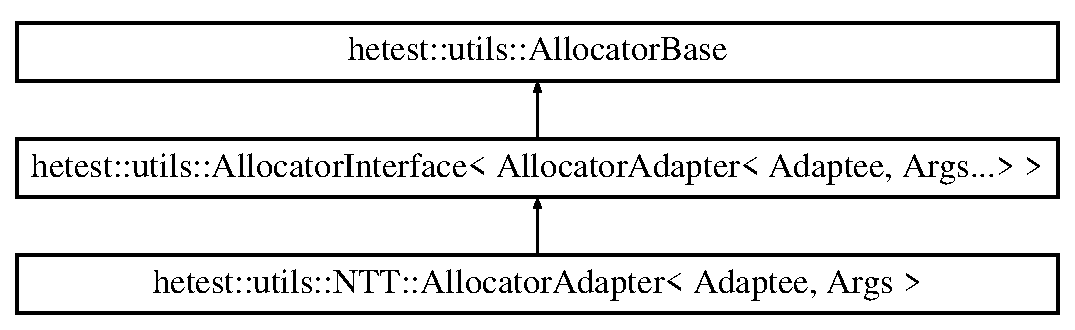
\includegraphics[height=3.000000cm]{structhetest_1_1utils_1_1NTT_1_1AllocatorAdapter}
\end{center}
\end{figure}
\subsection*{Public Member Functions}
\begin{DoxyCompactItemize}
\item 
\hyperlink{structhetest_1_1utils_1_1NTT_1_1AllocatorAdapter_acfe475e3767d7de45ae655e54d0846f0}{Allocator\-Adapter} (Adaptee \&\&\-\_\-a, Args \&\&...args)
\item 
\hyperlink{structhetest_1_1utils_1_1NTT_1_1AllocatorAdapter_a55c62e85f11443da9e79a0718a18ee2f}{Allocator\-Adapter} (const Adaptee \&\-\_\-a, Args \&...args)
\item 
void $\ast$ \hyperlink{structhetest_1_1utils_1_1NTT_1_1AllocatorAdapter_ac6b6542850337717e478d78477d89e6e}{allocate\-\_\-impl} (size\-\_\-t bytes\-\_\-count)
\item 
void \hyperlink{structhetest_1_1utils_1_1NTT_1_1AllocatorAdapter_af3dc9adfd717dc77aaa973e37642c4a6}{deallocate\-\_\-impl} (void $\ast$p, size\-\_\-t n)
\end{DoxyCompactItemize}


\subsection{Constructor \& Destructor Documentation}
\hypertarget{structhetest_1_1utils_1_1NTT_1_1AllocatorAdapter_acfe475e3767d7de45ae655e54d0846f0}{\index{hetest\-::utils\-::\-N\-T\-T\-::\-Allocator\-Adapter@{hetest\-::utils\-::\-N\-T\-T\-::\-Allocator\-Adapter}!Allocator\-Adapter@{Allocator\-Adapter}}
\index{Allocator\-Adapter@{Allocator\-Adapter}!hetest::utils::NTT::AllocatorAdapter@{hetest\-::utils\-::\-N\-T\-T\-::\-Allocator\-Adapter}}
\subsubsection[{Allocator\-Adapter}]{\setlength{\rightskip}{0pt plus 5cm}template$<$class Adaptee , class... Args$>$ {\bf hetest\-::utils\-::\-N\-T\-T\-::\-Allocator\-Adapter}$<$ Adaptee, Args $>$\-::{\bf Allocator\-Adapter} (
\begin{DoxyParamCaption}
\item[{Adaptee \&\&}]{\-\_\-a, }
\item[{Args \&\&...}]{args}
\end{DoxyParamCaption}
)\hspace{0.3cm}{\ttfamily [explicit]}}}\label{structhetest_1_1utils_1_1NTT_1_1AllocatorAdapter_acfe475e3767d7de45ae655e54d0846f0}
\hypertarget{structhetest_1_1utils_1_1NTT_1_1AllocatorAdapter_a55c62e85f11443da9e79a0718a18ee2f}{\index{hetest\-::utils\-::\-N\-T\-T\-::\-Allocator\-Adapter@{hetest\-::utils\-::\-N\-T\-T\-::\-Allocator\-Adapter}!Allocator\-Adapter@{Allocator\-Adapter}}
\index{Allocator\-Adapter@{Allocator\-Adapter}!hetest::utils::NTT::AllocatorAdapter@{hetest\-::utils\-::\-N\-T\-T\-::\-Allocator\-Adapter}}
\subsubsection[{Allocator\-Adapter}]{\setlength{\rightskip}{0pt plus 5cm}template$<$class Adaptee , class... Args$>$ {\bf hetest\-::utils\-::\-N\-T\-T\-::\-Allocator\-Adapter}$<$ Adaptee, Args $>$\-::{\bf Allocator\-Adapter} (
\begin{DoxyParamCaption}
\item[{const Adaptee \&}]{\-\_\-a, }
\item[{Args \&...}]{args}
\end{DoxyParamCaption}
)}}\label{structhetest_1_1utils_1_1NTT_1_1AllocatorAdapter_a55c62e85f11443da9e79a0718a18ee2f}


\subsection{Member Function Documentation}
\hypertarget{structhetest_1_1utils_1_1NTT_1_1AllocatorAdapter_ac6b6542850337717e478d78477d89e6e}{\index{hetest\-::utils\-::\-N\-T\-T\-::\-Allocator\-Adapter@{hetest\-::utils\-::\-N\-T\-T\-::\-Allocator\-Adapter}!allocate\-\_\-impl@{allocate\-\_\-impl}}
\index{allocate\-\_\-impl@{allocate\-\_\-impl}!hetest::utils::NTT::AllocatorAdapter@{hetest\-::utils\-::\-N\-T\-T\-::\-Allocator\-Adapter}}
\subsubsection[{allocate\-\_\-impl}]{\setlength{\rightskip}{0pt plus 5cm}template$<$class Adaptee , class... Args$>$ void$\ast$ {\bf hetest\-::utils\-::\-N\-T\-T\-::\-Allocator\-Adapter}$<$ Adaptee, Args $>$\-::allocate\-\_\-impl (
\begin{DoxyParamCaption}
\item[{size\-\_\-t}]{bytes\-\_\-count}
\end{DoxyParamCaption}
)}}\label{structhetest_1_1utils_1_1NTT_1_1AllocatorAdapter_ac6b6542850337717e478d78477d89e6e}
\hypertarget{structhetest_1_1utils_1_1NTT_1_1AllocatorAdapter_af3dc9adfd717dc77aaa973e37642c4a6}{\index{hetest\-::utils\-::\-N\-T\-T\-::\-Allocator\-Adapter@{hetest\-::utils\-::\-N\-T\-T\-::\-Allocator\-Adapter}!deallocate\-\_\-impl@{deallocate\-\_\-impl}}
\index{deallocate\-\_\-impl@{deallocate\-\_\-impl}!hetest::utils::NTT::AllocatorAdapter@{hetest\-::utils\-::\-N\-T\-T\-::\-Allocator\-Adapter}}
\subsubsection[{deallocate\-\_\-impl}]{\setlength{\rightskip}{0pt plus 5cm}template$<$class Adaptee , class... Args$>$ void {\bf hetest\-::utils\-::\-N\-T\-T\-::\-Allocator\-Adapter}$<$ Adaptee, Args $>$\-::deallocate\-\_\-impl (
\begin{DoxyParamCaption}
\item[{void $\ast$}]{p, }
\item[{size\-\_\-t}]{n}
\end{DoxyParamCaption}
)}}\label{structhetest_1_1utils_1_1NTT_1_1AllocatorAdapter_af3dc9adfd717dc77aaa973e37642c4a6}


The documentation for this struct was generated from the following file\-:\begin{DoxyCompactItemize}
\item 
\hyperlink{ntt_8hpp}{ntt.\-hpp}\end{DoxyCompactItemize}

\hypertarget{structhetest_1_1utils_1_1AllocatorBase}{\section{hetest\-:\-:utils\-:\-:Allocator\-Base Struct Reference}
\label{structhetest_1_1utils_1_1AllocatorBase}\index{hetest\-::utils\-::\-Allocator\-Base@{hetest\-::utils\-::\-Allocator\-Base}}
}


{\ttfamily \#include $<$utils-\/test.\-hpp$>$}

Inheritance diagram for hetest\-:\-:utils\-:\-:Allocator\-Base\-:\begin{figure}[H]
\begin{center}
\leavevmode
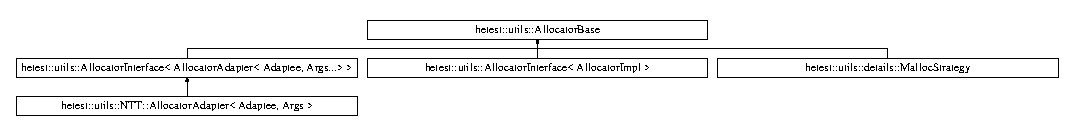
\includegraphics[height=1.327014cm]{structhetest_1_1utils_1_1AllocatorBase}
\end{center}
\end{figure}
\subsection*{Public Member Functions}
\begin{DoxyCompactItemize}
\item 
virtual \hyperlink{structhetest_1_1utils_1_1AllocatorBase_a8b16ff8d74578e0162706b8bbfa3751a}{$\sim$\-Allocator\-Base} () noexcept
\item 
virtual void $\ast$ \hyperlink{structhetest_1_1utils_1_1AllocatorBase_aa179ce655f57197104fce71166c17374}{allocate} (size\-\_\-t bytes\-\_\-count)=0
\item 
virtual void \hyperlink{structhetest_1_1utils_1_1AllocatorBase_ab9e3d2285da2861d0939afe26c6683e4}{deallocate} (void $\ast$p, size\-\_\-t n)=0
\end{DoxyCompactItemize}


\subsection{Constructor \& Destructor Documentation}
\hypertarget{structhetest_1_1utils_1_1AllocatorBase_a8b16ff8d74578e0162706b8bbfa3751a}{\index{hetest\-::utils\-::\-Allocator\-Base@{hetest\-::utils\-::\-Allocator\-Base}!$\sim$\-Allocator\-Base@{$\sim$\-Allocator\-Base}}
\index{$\sim$\-Allocator\-Base@{$\sim$\-Allocator\-Base}!hetest::utils::AllocatorBase@{hetest\-::utils\-::\-Allocator\-Base}}
\subsubsection[{$\sim$\-Allocator\-Base}]{\setlength{\rightskip}{0pt plus 5cm}virtual hetest\-::utils\-::\-Allocator\-Base\-::$\sim$\-Allocator\-Base (
\begin{DoxyParamCaption}
{}
\end{DoxyParamCaption}
)\hspace{0.3cm}{\ttfamily [inline]}, {\ttfamily [virtual]}, {\ttfamily [noexcept]}}}\label{structhetest_1_1utils_1_1AllocatorBase_a8b16ff8d74578e0162706b8bbfa3751a}


\subsection{Member Function Documentation}
\hypertarget{structhetest_1_1utils_1_1AllocatorBase_aa179ce655f57197104fce71166c17374}{\index{hetest\-::utils\-::\-Allocator\-Base@{hetest\-::utils\-::\-Allocator\-Base}!allocate@{allocate}}
\index{allocate@{allocate}!hetest::utils::AllocatorBase@{hetest\-::utils\-::\-Allocator\-Base}}
\subsubsection[{allocate}]{\setlength{\rightskip}{0pt plus 5cm}virtual void$\ast$ hetest\-::utils\-::\-Allocator\-Base\-::allocate (
\begin{DoxyParamCaption}
\item[{size\-\_\-t}]{bytes\-\_\-count}
\end{DoxyParamCaption}
)\hspace{0.3cm}{\ttfamily [pure virtual]}}}\label{structhetest_1_1utils_1_1AllocatorBase_aa179ce655f57197104fce71166c17374}


Implemented in \hyperlink{structhetest_1_1utils_1_1details_1_1MallocStrategy_a6e72b748596f8ba704363b1aa4d501d9}{hetest\-::utils\-::details\-::\-Malloc\-Strategy}, \hyperlink{structhetest_1_1utils_1_1AllocatorInterface_aa155e501b1e16984f8da9b1837597e66}{hetest\-::utils\-::\-Allocator\-Interface$<$ Allocator\-Impl $>$}, and \hyperlink{structhetest_1_1utils_1_1AllocatorInterface_aa155e501b1e16984f8da9b1837597e66}{hetest\-::utils\-::\-Allocator\-Interface$<$ Allocator\-Adapter$<$ Adaptee, Args...$>$ $>$}.

\hypertarget{structhetest_1_1utils_1_1AllocatorBase_ab9e3d2285da2861d0939afe26c6683e4}{\index{hetest\-::utils\-::\-Allocator\-Base@{hetest\-::utils\-::\-Allocator\-Base}!deallocate@{deallocate}}
\index{deallocate@{deallocate}!hetest::utils::AllocatorBase@{hetest\-::utils\-::\-Allocator\-Base}}
\subsubsection[{deallocate}]{\setlength{\rightskip}{0pt plus 5cm}virtual void hetest\-::utils\-::\-Allocator\-Base\-::deallocate (
\begin{DoxyParamCaption}
\item[{void $\ast$}]{p, }
\item[{size\-\_\-t}]{n}
\end{DoxyParamCaption}
)\hspace{0.3cm}{\ttfamily [pure virtual]}}}\label{structhetest_1_1utils_1_1AllocatorBase_ab9e3d2285da2861d0939afe26c6683e4}


Implemented in \hyperlink{structhetest_1_1utils_1_1details_1_1MallocStrategy_a86b2b253ec7d4da560da97f6d30e7325}{hetest\-::utils\-::details\-::\-Malloc\-Strategy}, \hyperlink{structhetest_1_1utils_1_1AllocatorInterface_a2d76269d7edd0d9cb65e6bfeffc24432}{hetest\-::utils\-::\-Allocator\-Interface$<$ Allocator\-Impl $>$}, and \hyperlink{structhetest_1_1utils_1_1AllocatorInterface_a2d76269d7edd0d9cb65e6bfeffc24432}{hetest\-::utils\-::\-Allocator\-Interface$<$ Allocator\-Adapter$<$ Adaptee, Args...$>$ $>$}.



The documentation for this struct was generated from the following file\-:\begin{DoxyCompactItemize}
\item 
\hyperlink{utils-test_8hpp}{utils-\/test.\-hpp}\end{DoxyCompactItemize}

\hypertarget{structhetest_1_1utils_1_1AllocatorInterface}{\section{hetest\-:\-:utils\-:\-:Allocator\-Interface$<$ Allocator\-Impl $>$ Struct Template Reference}
\label{structhetest_1_1utils_1_1AllocatorInterface}\index{hetest\-::utils\-::\-Allocator\-Interface$<$ Allocator\-Impl $>$@{hetest\-::utils\-::\-Allocator\-Interface$<$ Allocator\-Impl $>$}}
}


{\ttfamily \#include $<$utils-\/test.\-hpp$>$}

Inheritance diagram for hetest\-:\-:utils\-:\-:Allocator\-Interface$<$ Allocator\-Impl $>$\-:\begin{figure}[H]
\begin{center}
\leavevmode
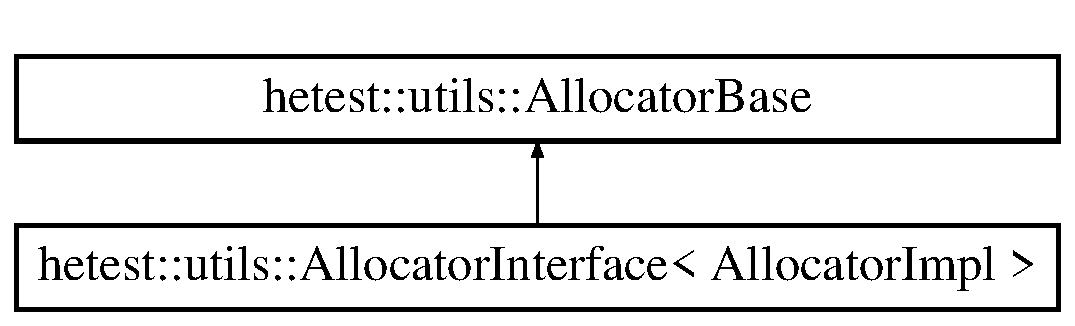
\includegraphics[height=2.000000cm]{structhetest_1_1utils_1_1AllocatorInterface}
\end{center}
\end{figure}
\subsection*{Public Member Functions}
\begin{DoxyCompactItemize}
\item 
void $\ast$ \hyperlink{structhetest_1_1utils_1_1AllocatorInterface_aa155e501b1e16984f8da9b1837597e66}{allocate} (size\-\_\-t bytes\-\_\-count) override
\item 
void \hyperlink{structhetest_1_1utils_1_1AllocatorInterface_a2d76269d7edd0d9cb65e6bfeffc24432}{deallocate} (void $\ast$p, size\-\_\-t n) override
\end{DoxyCompactItemize}


\subsection{Member Function Documentation}
\hypertarget{structhetest_1_1utils_1_1AllocatorInterface_aa155e501b1e16984f8da9b1837597e66}{\index{hetest\-::utils\-::\-Allocator\-Interface@{hetest\-::utils\-::\-Allocator\-Interface}!allocate@{allocate}}
\index{allocate@{allocate}!hetest::utils::AllocatorInterface@{hetest\-::utils\-::\-Allocator\-Interface}}
\subsubsection[{allocate}]{\setlength{\rightskip}{0pt plus 5cm}template$<$class Allocator\-Impl$>$ void$\ast$ {\bf hetest\-::utils\-::\-Allocator\-Interface}$<$ Allocator\-Impl $>$\-::allocate (
\begin{DoxyParamCaption}
\item[{size\-\_\-t}]{bytes\-\_\-count}
\end{DoxyParamCaption}
)\hspace{0.3cm}{\ttfamily [inline]}, {\ttfamily [override]}, {\ttfamily [virtual]}}}\label{structhetest_1_1utils_1_1AllocatorInterface_aa155e501b1e16984f8da9b1837597e66}


Implements \hyperlink{structhetest_1_1utils_1_1AllocatorBase_aa179ce655f57197104fce71166c17374}{hetest\-::utils\-::\-Allocator\-Base}.

\hypertarget{structhetest_1_1utils_1_1AllocatorInterface_a2d76269d7edd0d9cb65e6bfeffc24432}{\index{hetest\-::utils\-::\-Allocator\-Interface@{hetest\-::utils\-::\-Allocator\-Interface}!deallocate@{deallocate}}
\index{deallocate@{deallocate}!hetest::utils::AllocatorInterface@{hetest\-::utils\-::\-Allocator\-Interface}}
\subsubsection[{deallocate}]{\setlength{\rightskip}{0pt plus 5cm}template$<$class Allocator\-Impl$>$ void {\bf hetest\-::utils\-::\-Allocator\-Interface}$<$ Allocator\-Impl $>$\-::deallocate (
\begin{DoxyParamCaption}
\item[{void $\ast$}]{p, }
\item[{size\-\_\-t}]{n}
\end{DoxyParamCaption}
)\hspace{0.3cm}{\ttfamily [inline]}, {\ttfamily [override]}, {\ttfamily [virtual]}}}\label{structhetest_1_1utils_1_1AllocatorInterface_a2d76269d7edd0d9cb65e6bfeffc24432}


Implements \hyperlink{structhetest_1_1utils_1_1AllocatorBase_ab9e3d2285da2861d0939afe26c6683e4}{hetest\-::utils\-::\-Allocator\-Base}.



The documentation for this struct was generated from the following file\-:\begin{DoxyCompactItemize}
\item 
\hyperlink{utils-test_8hpp}{utils-\/test.\-hpp}\end{DoxyCompactItemize}

\hypertarget{classintel_1_1hexl_1_1fpga_1_1Buffer}{\section{intel\-:\-:hexl\-:\-:fpga\-:\-:Buffer Class Reference}
\label{classintel_1_1hexl_1_1fpga_1_1Buffer}\index{intel\-::hexl\-::fpga\-::\-Buffer@{intel\-::hexl\-::fpga\-::\-Buffer}}
}


Struct \hyperlink{classintel_1_1hexl_1_1fpga_1_1Buffer}{Buffer} Structure containing information for the polynomial operations.  




{\ttfamily \#include $<$fpga.\-h$>$}

\subsection*{Public Member Functions}
\begin{DoxyCompactItemize}
\item 
\hyperlink{classintel_1_1hexl_1_1fpga_1_1Buffer_ad6b70e490557e9c8035810efdb5fb770}{Buffer} (uint64\-\_\-t capacity, uint64\-\_\-t n\-\_\-batch\-\_\-dyadic\-\_\-multiply, uint64\-\_\-t n\-\_\-batch\-\_\-ntt, uint64\-\_\-t n\-\_\-batch\-\_\-intt)
\item 
void \hyperlink{classintel_1_1hexl_1_1fpga_1_1Buffer_a6644861e903def2ff1aef60c94f4a8f6}{push} (\hyperlink{structintel_1_1hexl_1_1fpga_1_1Object}{Object} $\ast$obj)
\item 
\hyperlink{structintel_1_1hexl_1_1fpga_1_1Object}{Object} $\ast$ \hyperlink{classintel_1_1hexl_1_1fpga_1_1Buffer_abf9ee3bd20574de86aae2dc8af3913be}{front} ()
\item 
std\-::vector$<$ \hyperlink{structintel_1_1hexl_1_1fpga_1_1Object}{Object} $\ast$ $>$ \hyperlink{classintel_1_1hexl_1_1fpga_1_1Buffer_ac60152c34dc6d5ac1275db07293fc7dc}{pop} ()
\item 
uint64\-\_\-t \hyperlink{classintel_1_1hexl_1_1fpga_1_1Buffer_a03dbef5789ed9c28bd1b63b35164ab41}{size} ()
\item 
uint64\-\_\-t \hyperlink{classintel_1_1hexl_1_1fpga_1_1Buffer_a346da8900c5d0f689de15c754ff22095}{get\-\_\-worksize\-\_\-\-Dyadic\-Multiply} () const 
\item 
uint64\-\_\-t \hyperlink{classintel_1_1hexl_1_1fpga_1_1Buffer_a7814dc29476fa0be598a8f2f99043024}{get\-\_\-worksize\-\_\-\-N\-T\-T} () const 
\item 
uint64\-\_\-t \hyperlink{classintel_1_1hexl_1_1fpga_1_1Buffer_a7147f2da3c6cbeeaf13f70d725622a87}{get\-\_\-worksize\-\_\-\-I\-N\-T\-T} () const 
\item 
void \hyperlink{classintel_1_1hexl_1_1fpga_1_1Buffer_a3ed2fb00d1e5eb733162588d30a395df}{set\-\_\-worksize\-\_\-\-Dyadic\-Multiply} (uint64\-\_\-t ws)
\item 
void \hyperlink{classintel_1_1hexl_1_1fpga_1_1Buffer_aa6c582210106d0e189630dbd47a2b613}{set\-\_\-worksize\-\_\-\-N\-T\-T} (uint64\-\_\-t ws)
\item 
void \hyperlink{classintel_1_1hexl_1_1fpga_1_1Buffer_aa9d41687d0a35d75bb12b96373a3ddf4}{set\-\_\-worksize\-\_\-\-I\-N\-T\-T} (uint64\-\_\-t ws)
\end{DoxyCompactItemize}


\subsection{Detailed Description}
Struct \hyperlink{classintel_1_1hexl_1_1fpga_1_1Buffer}{Buffer} Structure containing information for the polynomial operations. 


\begin{DoxyParams}[1]{Parameters}
\mbox{\tt in}  & {\em capacity} & of the buffer \\
\hline
\mbox{\tt in}  & {\em n\-\_\-batch\-\_\-dyadic\-\_\-multiply} & batch size for the multiplication \\
\hline
\mbox{\tt in}  & {\em n\-\_\-batch\-\_\-ntt} & batch size for the Number Theoretical Transform \\
\hline
\mbox{\tt in}  & {\em n\-\_\-batch\-\_\-intt} & batch size for the inverse Number Theoretical Transform \\
\hline
\mbox{\tt in}  & {\em total\-\_\-worksize\-\_\-\-Dyadic\-Multiply} & stores the worksize for the multiplication \\
\hline
\mbox{\tt in}  & {\em num\-\_\-\-Dyadic\-Multiply} & stores the number of multiplications to be performed \\
\hline
\mbox{\tt in}  & {\em total\-\_\-worksize\-\_\-\-N\-T\-T} & stores the worksize for the N\-T\-T \\
\hline
\mbox{\tt in}  & {\em num\-\_\-\-N\-T\-T} & stores the number of N\-T\-T to be performed \\
\hline
\mbox{\tt in}  & {\em total\-\_\-worksize\-\_\-\-I\-N\-T\-T} & stores the worksize for the I\-N\-T\-T \\
\hline
\mbox{\tt in}  & {\em num\-\_\-\-I\-N\-T\-T} & stores the number of I\-N\-T\-T to be performed  push pushes an \hyperlink{structintel_1_1hexl_1_1fpga_1_1Object}{Object} in the structure  front returns the front \hyperlink{structintel_1_1hexl_1_1fpga_1_1Object}{Object} of the structure  pop pops the front \hyperlink{structintel_1_1hexl_1_1fpga_1_1Object}{Object} out of the structure  size returns the size of the structure  get\-\_\-worksize\-\_\-\-Dyadic\-Multiply returns the worksize of Dyadic\-Multiply  get\-\_\-worksize\-\_\-\-N\-T\-T returns the worksize of N\-T\-T  get\-\_\-worksize\-\_\-\-I\-N\-T\-T returns the worksize of I\-N\-T\-T  set\-\_\-worksize\-\_\-\-Dyadic\-Multiply sets the worksize of Dyadic\-Multiply  set\-\_\-worksize\-\_\-\-N\-T\-T sets the worksize of N\-T\-T  set\-\_\-worksize\-\_\-\-I\-N\-T\-T setsthe worksize of I\-N\-T\-T \\
\hline
\end{DoxyParams}


\subsection{Constructor \& Destructor Documentation}
\hypertarget{classintel_1_1hexl_1_1fpga_1_1Buffer_ad6b70e490557e9c8035810efdb5fb770}{\index{intel\-::hexl\-::fpga\-::\-Buffer@{intel\-::hexl\-::fpga\-::\-Buffer}!Buffer@{Buffer}}
\index{Buffer@{Buffer}!intel::hexl::fpga::Buffer@{intel\-::hexl\-::fpga\-::\-Buffer}}
\subsubsection[{Buffer}]{\setlength{\rightskip}{0pt plus 5cm}intel\-::hexl\-::fpga\-::\-Buffer\-::\-Buffer (
\begin{DoxyParamCaption}
\item[{uint64\-\_\-t}]{capacity, }
\item[{uint64\-\_\-t}]{n\-\_\-batch\-\_\-dyadic\-\_\-multiply, }
\item[{uint64\-\_\-t}]{n\-\_\-batch\-\_\-ntt, }
\item[{uint64\-\_\-t}]{n\-\_\-batch\-\_\-intt}
\end{DoxyParamCaption}
)\hspace{0.3cm}{\ttfamily [inline]}}}\label{classintel_1_1hexl_1_1fpga_1_1Buffer_ad6b70e490557e9c8035810efdb5fb770}


\subsection{Member Function Documentation}
\hypertarget{classintel_1_1hexl_1_1fpga_1_1Buffer_abf9ee3bd20574de86aae2dc8af3913be}{\index{intel\-::hexl\-::fpga\-::\-Buffer@{intel\-::hexl\-::fpga\-::\-Buffer}!front@{front}}
\index{front@{front}!intel::hexl::fpga::Buffer@{intel\-::hexl\-::fpga\-::\-Buffer}}
\subsubsection[{front}]{\setlength{\rightskip}{0pt plus 5cm}{\bf Object}$\ast$ intel\-::hexl\-::fpga\-::\-Buffer\-::front (
\begin{DoxyParamCaption}
{}
\end{DoxyParamCaption}
)}}\label{classintel_1_1hexl_1_1fpga_1_1Buffer_abf9ee3bd20574de86aae2dc8af3913be}
\hypertarget{classintel_1_1hexl_1_1fpga_1_1Buffer_a346da8900c5d0f689de15c754ff22095}{\index{intel\-::hexl\-::fpga\-::\-Buffer@{intel\-::hexl\-::fpga\-::\-Buffer}!get\-\_\-worksize\-\_\-\-Dyadic\-Multiply@{get\-\_\-worksize\-\_\-\-Dyadic\-Multiply}}
\index{get\-\_\-worksize\-\_\-\-Dyadic\-Multiply@{get\-\_\-worksize\-\_\-\-Dyadic\-Multiply}!intel::hexl::fpga::Buffer@{intel\-::hexl\-::fpga\-::\-Buffer}}
\subsubsection[{get\-\_\-worksize\-\_\-\-Dyadic\-Multiply}]{\setlength{\rightskip}{0pt plus 5cm}uint64\-\_\-t intel\-::hexl\-::fpga\-::\-Buffer\-::get\-\_\-worksize\-\_\-\-Dyadic\-Multiply (
\begin{DoxyParamCaption}
{}
\end{DoxyParamCaption}
) const\hspace{0.3cm}{\ttfamily [inline]}}}\label{classintel_1_1hexl_1_1fpga_1_1Buffer_a346da8900c5d0f689de15c754ff22095}
\hypertarget{classintel_1_1hexl_1_1fpga_1_1Buffer_a7147f2da3c6cbeeaf13f70d725622a87}{\index{intel\-::hexl\-::fpga\-::\-Buffer@{intel\-::hexl\-::fpga\-::\-Buffer}!get\-\_\-worksize\-\_\-\-I\-N\-T\-T@{get\-\_\-worksize\-\_\-\-I\-N\-T\-T}}
\index{get\-\_\-worksize\-\_\-\-I\-N\-T\-T@{get\-\_\-worksize\-\_\-\-I\-N\-T\-T}!intel::hexl::fpga::Buffer@{intel\-::hexl\-::fpga\-::\-Buffer}}
\subsubsection[{get\-\_\-worksize\-\_\-\-I\-N\-T\-T}]{\setlength{\rightskip}{0pt plus 5cm}uint64\-\_\-t intel\-::hexl\-::fpga\-::\-Buffer\-::get\-\_\-worksize\-\_\-\-I\-N\-T\-T (
\begin{DoxyParamCaption}
{}
\end{DoxyParamCaption}
) const\hspace{0.3cm}{\ttfamily [inline]}}}\label{classintel_1_1hexl_1_1fpga_1_1Buffer_a7147f2da3c6cbeeaf13f70d725622a87}
\hypertarget{classintel_1_1hexl_1_1fpga_1_1Buffer_a7814dc29476fa0be598a8f2f99043024}{\index{intel\-::hexl\-::fpga\-::\-Buffer@{intel\-::hexl\-::fpga\-::\-Buffer}!get\-\_\-worksize\-\_\-\-N\-T\-T@{get\-\_\-worksize\-\_\-\-N\-T\-T}}
\index{get\-\_\-worksize\-\_\-\-N\-T\-T@{get\-\_\-worksize\-\_\-\-N\-T\-T}!intel::hexl::fpga::Buffer@{intel\-::hexl\-::fpga\-::\-Buffer}}
\subsubsection[{get\-\_\-worksize\-\_\-\-N\-T\-T}]{\setlength{\rightskip}{0pt plus 5cm}uint64\-\_\-t intel\-::hexl\-::fpga\-::\-Buffer\-::get\-\_\-worksize\-\_\-\-N\-T\-T (
\begin{DoxyParamCaption}
{}
\end{DoxyParamCaption}
) const\hspace{0.3cm}{\ttfamily [inline]}}}\label{classintel_1_1hexl_1_1fpga_1_1Buffer_a7814dc29476fa0be598a8f2f99043024}
\hypertarget{classintel_1_1hexl_1_1fpga_1_1Buffer_ac60152c34dc6d5ac1275db07293fc7dc}{\index{intel\-::hexl\-::fpga\-::\-Buffer@{intel\-::hexl\-::fpga\-::\-Buffer}!pop@{pop}}
\index{pop@{pop}!intel::hexl::fpga::Buffer@{intel\-::hexl\-::fpga\-::\-Buffer}}
\subsubsection[{pop}]{\setlength{\rightskip}{0pt plus 5cm}std\-::vector$<${\bf Object}$\ast$$>$ intel\-::hexl\-::fpga\-::\-Buffer\-::pop (
\begin{DoxyParamCaption}
{}
\end{DoxyParamCaption}
)}}\label{classintel_1_1hexl_1_1fpga_1_1Buffer_ac60152c34dc6d5ac1275db07293fc7dc}
\hypertarget{classintel_1_1hexl_1_1fpga_1_1Buffer_a6644861e903def2ff1aef60c94f4a8f6}{\index{intel\-::hexl\-::fpga\-::\-Buffer@{intel\-::hexl\-::fpga\-::\-Buffer}!push@{push}}
\index{push@{push}!intel::hexl::fpga::Buffer@{intel\-::hexl\-::fpga\-::\-Buffer}}
\subsubsection[{push}]{\setlength{\rightskip}{0pt plus 5cm}void intel\-::hexl\-::fpga\-::\-Buffer\-::push (
\begin{DoxyParamCaption}
\item[{{\bf Object} $\ast$}]{obj}
\end{DoxyParamCaption}
)}}\label{classintel_1_1hexl_1_1fpga_1_1Buffer_a6644861e903def2ff1aef60c94f4a8f6}
\hypertarget{classintel_1_1hexl_1_1fpga_1_1Buffer_a3ed2fb00d1e5eb733162588d30a395df}{\index{intel\-::hexl\-::fpga\-::\-Buffer@{intel\-::hexl\-::fpga\-::\-Buffer}!set\-\_\-worksize\-\_\-\-Dyadic\-Multiply@{set\-\_\-worksize\-\_\-\-Dyadic\-Multiply}}
\index{set\-\_\-worksize\-\_\-\-Dyadic\-Multiply@{set\-\_\-worksize\-\_\-\-Dyadic\-Multiply}!intel::hexl::fpga::Buffer@{intel\-::hexl\-::fpga\-::\-Buffer}}
\subsubsection[{set\-\_\-worksize\-\_\-\-Dyadic\-Multiply}]{\setlength{\rightskip}{0pt plus 5cm}void intel\-::hexl\-::fpga\-::\-Buffer\-::set\-\_\-worksize\-\_\-\-Dyadic\-Multiply (
\begin{DoxyParamCaption}
\item[{uint64\-\_\-t}]{ws}
\end{DoxyParamCaption}
)\hspace{0.3cm}{\ttfamily [inline]}}}\label{classintel_1_1hexl_1_1fpga_1_1Buffer_a3ed2fb00d1e5eb733162588d30a395df}
\hypertarget{classintel_1_1hexl_1_1fpga_1_1Buffer_aa9d41687d0a35d75bb12b96373a3ddf4}{\index{intel\-::hexl\-::fpga\-::\-Buffer@{intel\-::hexl\-::fpga\-::\-Buffer}!set\-\_\-worksize\-\_\-\-I\-N\-T\-T@{set\-\_\-worksize\-\_\-\-I\-N\-T\-T}}
\index{set\-\_\-worksize\-\_\-\-I\-N\-T\-T@{set\-\_\-worksize\-\_\-\-I\-N\-T\-T}!intel::hexl::fpga::Buffer@{intel\-::hexl\-::fpga\-::\-Buffer}}
\subsubsection[{set\-\_\-worksize\-\_\-\-I\-N\-T\-T}]{\setlength{\rightskip}{0pt plus 5cm}void intel\-::hexl\-::fpga\-::\-Buffer\-::set\-\_\-worksize\-\_\-\-I\-N\-T\-T (
\begin{DoxyParamCaption}
\item[{uint64\-\_\-t}]{ws}
\end{DoxyParamCaption}
)\hspace{0.3cm}{\ttfamily [inline]}}}\label{classintel_1_1hexl_1_1fpga_1_1Buffer_aa9d41687d0a35d75bb12b96373a3ddf4}
\hypertarget{classintel_1_1hexl_1_1fpga_1_1Buffer_aa6c582210106d0e189630dbd47a2b613}{\index{intel\-::hexl\-::fpga\-::\-Buffer@{intel\-::hexl\-::fpga\-::\-Buffer}!set\-\_\-worksize\-\_\-\-N\-T\-T@{set\-\_\-worksize\-\_\-\-N\-T\-T}}
\index{set\-\_\-worksize\-\_\-\-N\-T\-T@{set\-\_\-worksize\-\_\-\-N\-T\-T}!intel::hexl::fpga::Buffer@{intel\-::hexl\-::fpga\-::\-Buffer}}
\subsubsection[{set\-\_\-worksize\-\_\-\-N\-T\-T}]{\setlength{\rightskip}{0pt plus 5cm}void intel\-::hexl\-::fpga\-::\-Buffer\-::set\-\_\-worksize\-\_\-\-N\-T\-T (
\begin{DoxyParamCaption}
\item[{uint64\-\_\-t}]{ws}
\end{DoxyParamCaption}
)\hspace{0.3cm}{\ttfamily [inline]}}}\label{classintel_1_1hexl_1_1fpga_1_1Buffer_aa6c582210106d0e189630dbd47a2b613}
\hypertarget{classintel_1_1hexl_1_1fpga_1_1Buffer_a03dbef5789ed9c28bd1b63b35164ab41}{\index{intel\-::hexl\-::fpga\-::\-Buffer@{intel\-::hexl\-::fpga\-::\-Buffer}!size@{size}}
\index{size@{size}!intel::hexl::fpga::Buffer@{intel\-::hexl\-::fpga\-::\-Buffer}}
\subsubsection[{size}]{\setlength{\rightskip}{0pt plus 5cm}uint64\-\_\-t intel\-::hexl\-::fpga\-::\-Buffer\-::size (
\begin{DoxyParamCaption}
{}
\end{DoxyParamCaption}
)}}\label{classintel_1_1hexl_1_1fpga_1_1Buffer_a03dbef5789ed9c28bd1b63b35164ab41}


The documentation for this class was generated from the following file\-:\begin{DoxyCompactItemize}
\item 
\hyperlink{fpga_8h}{fpga.\-h}\end{DoxyCompactItemize}

\hypertarget{structhetest_1_1utils_1_1details_1_1CustomAllocStrategy}{\section{hetest\-:\-:utils\-:\-:details\-:\-:Custom\-Alloc\-Strategy Struct Reference}
\label{structhetest_1_1utils_1_1details_1_1CustomAllocStrategy}\index{hetest\-::utils\-::details\-::\-Custom\-Alloc\-Strategy@{hetest\-::utils\-::details\-::\-Custom\-Alloc\-Strategy}}
}


{\ttfamily \#include $<$utils-\/test.\-hpp$>$}

\subsection*{Public Member Functions}
\begin{DoxyCompactItemize}
\item 
\hyperlink{structhetest_1_1utils_1_1details_1_1CustomAllocStrategy_aecbed5a7bad355a6ac9c72dcf88c9936}{Custom\-Alloc\-Strategy} (std\-::shared\-\_\-ptr$<$ \hyperlink{structhetest_1_1utils_1_1AllocatorBase}{Allocator\-Base} $>$ impl)
\item 
void $\ast$ \hyperlink{structhetest_1_1utils_1_1details_1_1CustomAllocStrategy_aab5db3cb69c7135a945a8b3e094645a3}{allocate\-\_\-memory} (size\-\_\-t bytes\-\_\-count)
\item 
void \hyperlink{structhetest_1_1utils_1_1details_1_1CustomAllocStrategy_ac37a17b014a233a6dd134704c6d072ac}{deallocate\-\_\-memory} (void $\ast$p, size\-\_\-t n)
\end{DoxyCompactItemize}


\subsection{Constructor \& Destructor Documentation}
\hypertarget{structhetest_1_1utils_1_1details_1_1CustomAllocStrategy_aecbed5a7bad355a6ac9c72dcf88c9936}{\index{hetest\-::utils\-::details\-::\-Custom\-Alloc\-Strategy@{hetest\-::utils\-::details\-::\-Custom\-Alloc\-Strategy}!Custom\-Alloc\-Strategy@{Custom\-Alloc\-Strategy}}
\index{Custom\-Alloc\-Strategy@{Custom\-Alloc\-Strategy}!hetest::utils::details::CustomAllocStrategy@{hetest\-::utils\-::details\-::\-Custom\-Alloc\-Strategy}}
\subsubsection[{Custom\-Alloc\-Strategy}]{\setlength{\rightskip}{0pt plus 5cm}hetest\-::utils\-::details\-::\-Custom\-Alloc\-Strategy\-::\-Custom\-Alloc\-Strategy (
\begin{DoxyParamCaption}
\item[{std\-::shared\-\_\-ptr$<$ {\bf Allocator\-Base} $>$}]{impl}
\end{DoxyParamCaption}
)\hspace{0.3cm}{\ttfamily [inline]}, {\ttfamily [explicit]}}}\label{structhetest_1_1utils_1_1details_1_1CustomAllocStrategy_aecbed5a7bad355a6ac9c72dcf88c9936}


\subsection{Member Function Documentation}
\hypertarget{structhetest_1_1utils_1_1details_1_1CustomAllocStrategy_aab5db3cb69c7135a945a8b3e094645a3}{\index{hetest\-::utils\-::details\-::\-Custom\-Alloc\-Strategy@{hetest\-::utils\-::details\-::\-Custom\-Alloc\-Strategy}!allocate\-\_\-memory@{allocate\-\_\-memory}}
\index{allocate\-\_\-memory@{allocate\-\_\-memory}!hetest::utils::details::CustomAllocStrategy@{hetest\-::utils\-::details\-::\-Custom\-Alloc\-Strategy}}
\subsubsection[{allocate\-\_\-memory}]{\setlength{\rightskip}{0pt plus 5cm}void$\ast$ hetest\-::utils\-::details\-::\-Custom\-Alloc\-Strategy\-::allocate\-\_\-memory (
\begin{DoxyParamCaption}
\item[{size\-\_\-t}]{bytes\-\_\-count}
\end{DoxyParamCaption}
)\hspace{0.3cm}{\ttfamily [inline]}}}\label{structhetest_1_1utils_1_1details_1_1CustomAllocStrategy_aab5db3cb69c7135a945a8b3e094645a3}
\hypertarget{structhetest_1_1utils_1_1details_1_1CustomAllocStrategy_ac37a17b014a233a6dd134704c6d072ac}{\index{hetest\-::utils\-::details\-::\-Custom\-Alloc\-Strategy@{hetest\-::utils\-::details\-::\-Custom\-Alloc\-Strategy}!deallocate\-\_\-memory@{deallocate\-\_\-memory}}
\index{deallocate\-\_\-memory@{deallocate\-\_\-memory}!hetest::utils::details::CustomAllocStrategy@{hetest\-::utils\-::details\-::\-Custom\-Alloc\-Strategy}}
\subsubsection[{deallocate\-\_\-memory}]{\setlength{\rightskip}{0pt plus 5cm}void hetest\-::utils\-::details\-::\-Custom\-Alloc\-Strategy\-::deallocate\-\_\-memory (
\begin{DoxyParamCaption}
\item[{void $\ast$}]{p, }
\item[{size\-\_\-t}]{n}
\end{DoxyParamCaption}
)\hspace{0.3cm}{\ttfamily [inline]}}}\label{structhetest_1_1utils_1_1details_1_1CustomAllocStrategy_ac37a17b014a233a6dd134704c6d072ac}


The documentation for this struct was generated from the following file\-:\begin{DoxyCompactItemize}
\item 
\hyperlink{utils-test_8hpp}{utils-\/test.\-hpp}\end{DoxyCompactItemize}

\hypertarget{classintel_1_1hexl_1_1fpga_1_1Device}{\section{intel\-:\-:hexl\-:\-:fpga\-:\-:Device Class Reference}
\label{classintel_1_1hexl_1_1fpga_1_1Device}\index{intel\-::hexl\-::fpga\-::\-Device@{intel\-::hexl\-::fpga\-::\-Device}}
}


Class \hyperlink{classintel_1_1hexl_1_1fpga_1_1Device}{Device}.  




{\ttfamily \#include $<$fpga.\-h$>$}

\subsection*{Public Member Functions}
\begin{DoxyCompactItemize}
\item 
\hyperlink{classintel_1_1hexl_1_1fpga_1_1Device_a444b8a5c92f908f0e61cb5c3513e36a9}{Device} (const cl\-\_\-device\-\_\-id \&device, \hyperlink{classintel_1_1hexl_1_1fpga_1_1Buffer}{Buffer} \&buffer, std\-::shared\-\_\-future$<$ bool $>$ exit\-\_\-signal, uint64\-\_\-t coeff\-\_\-size, uint32\-\_\-t modulus\-\_\-size, uint64\-\_\-t batch\-\_\-size\-\_\-dyadic\-\_\-multiply, uint64\-\_\-t batch\-\_\-size\-\_\-ntt, uint64\-\_\-t batch\-\_\-size\-\_\-intt, uint32\-\_\-t debug)
\item 
\hyperlink{classintel_1_1hexl_1_1fpga_1_1Device_ad7adf350f85c3d0b66607424d3281d5f}{$\sim$\-Device} ()
\item 
void \hyperlink{classintel_1_1hexl_1_1fpga_1_1Device_a91c2dde32f856517ba1f90e6191d2850}{run} ()
\end{DoxyCompactItemize}


\subsection{Detailed Description}
Class \hyperlink{classintel_1_1hexl_1_1fpga_1_1Device}{Device}. 

\hyperlink{classintel_1_1hexl_1_1fpga_1_1Device}{Device} Constructor 
\begin{DoxyParams}[1]{Parameters}
\mbox{\tt in}  & {\em device} & choice between emulation and F\-P\-G\-A \\
\hline
\mbox{\tt in}  & {\em buffer} & memory blob where objects are stored \\
\hline
\mbox{\tt in}  & {\em exit\-\_\-signal} & flag signaling data available \\
\hline
\mbox{\tt in}  & {\em coeff\-\_\-size} & polynomial coefficient size \\
\hline
\mbox{\tt in}  & {\em modulus\-\_\-size} & modulus size \\
\hline
\mbox{\tt in}  & {\em batch\-\_\-size\-\_\-dyadic\-\_\-multiply} & batch size for the multiplication operation \\
\hline
\mbox{\tt in}  & {\em batch\-\_\-size\-\_\-ntt} & batch size for the N\-T\-T operation \\
\hline
\mbox{\tt in}  & {\em batch\-\_\-size\-\_\-intt} & batch size for the I\-N\-T\-T operation \\
\hline
\mbox{\tt in}  & {\em debug} & flag indicating debug mode\\
\hline
\end{DoxyParams}
run function to launch the operation on the F\-P\-G\-A 

\subsection{Constructor \& Destructor Documentation}
\hypertarget{classintel_1_1hexl_1_1fpga_1_1Device_a444b8a5c92f908f0e61cb5c3513e36a9}{\index{intel\-::hexl\-::fpga\-::\-Device@{intel\-::hexl\-::fpga\-::\-Device}!Device@{Device}}
\index{Device@{Device}!intel::hexl::fpga::Device@{intel\-::hexl\-::fpga\-::\-Device}}
\subsubsection[{Device}]{\setlength{\rightskip}{0pt plus 5cm}intel\-::hexl\-::fpga\-::\-Device\-::\-Device (
\begin{DoxyParamCaption}
\item[{const cl\-\_\-device\-\_\-id \&}]{device, }
\item[{{\bf Buffer} \&}]{buffer, }
\item[{std\-::shared\-\_\-future$<$ bool $>$}]{exit\-\_\-signal, }
\item[{uint64\-\_\-t}]{coeff\-\_\-size, }
\item[{uint32\-\_\-t}]{modulus\-\_\-size, }
\item[{uint64\-\_\-t}]{batch\-\_\-size\-\_\-dyadic\-\_\-multiply, }
\item[{uint64\-\_\-t}]{batch\-\_\-size\-\_\-ntt, }
\item[{uint64\-\_\-t}]{batch\-\_\-size\-\_\-intt, }
\item[{uint32\-\_\-t}]{debug}
\end{DoxyParamCaption}
)}}\label{classintel_1_1hexl_1_1fpga_1_1Device_a444b8a5c92f908f0e61cb5c3513e36a9}
\hypertarget{classintel_1_1hexl_1_1fpga_1_1Device_ad7adf350f85c3d0b66607424d3281d5f}{\index{intel\-::hexl\-::fpga\-::\-Device@{intel\-::hexl\-::fpga\-::\-Device}!$\sim$\-Device@{$\sim$\-Device}}
\index{$\sim$\-Device@{$\sim$\-Device}!intel::hexl::fpga::Device@{intel\-::hexl\-::fpga\-::\-Device}}
\subsubsection[{$\sim$\-Device}]{\setlength{\rightskip}{0pt plus 5cm}intel\-::hexl\-::fpga\-::\-Device\-::$\sim$\-Device (
\begin{DoxyParamCaption}
{}
\end{DoxyParamCaption}
)}}\label{classintel_1_1hexl_1_1fpga_1_1Device_ad7adf350f85c3d0b66607424d3281d5f}


\subsection{Member Function Documentation}
\hypertarget{classintel_1_1hexl_1_1fpga_1_1Device_a91c2dde32f856517ba1f90e6191d2850}{\index{intel\-::hexl\-::fpga\-::\-Device@{intel\-::hexl\-::fpga\-::\-Device}!run@{run}}
\index{run@{run}!intel::hexl::fpga::Device@{intel\-::hexl\-::fpga\-::\-Device}}
\subsubsection[{run}]{\setlength{\rightskip}{0pt plus 5cm}void intel\-::hexl\-::fpga\-::\-Device\-::run (
\begin{DoxyParamCaption}
{}
\end{DoxyParamCaption}
)}}\label{classintel_1_1hexl_1_1fpga_1_1Device_a91c2dde32f856517ba1f90e6191d2850}


The documentation for this class was generated from the following file\-:\begin{DoxyCompactItemize}
\item 
\hyperlink{fpga_8h}{fpga.\-h}\end{DoxyCompactItemize}

\hypertarget{classintel_1_1hexl_1_1fpga_1_1DevicePool}{\section{intel\-:\-:hexl\-:\-:fpga\-:\-:Device\-Pool Class Reference}
\label{classintel_1_1hexl_1_1fpga_1_1DevicePool}\index{intel\-::hexl\-::fpga\-::\-Device\-Pool@{intel\-::hexl\-::fpga\-::\-Device\-Pool}}
}


Class \hyperlink{classintel_1_1hexl_1_1fpga_1_1DevicePool}{Device\-Pool}.  




{\ttfamily \#include $<$fpga.\-h$>$}

\subsection*{Public Member Functions}
\begin{DoxyCompactItemize}
\item 
\hyperlink{classintel_1_1hexl_1_1fpga_1_1DevicePool_a3561da094204c47678f022a2d5ac26ab}{Device\-Pool} (int choice, \hyperlink{classintel_1_1hexl_1_1fpga_1_1Buffer}{Buffer} \&buffer, std\-::future$<$ bool $>$ \&exit\-\_\-signal, uint64\-\_\-t coeff\-\_\-size, uint32\-\_\-t modulus\-\_\-size, uint64\-\_\-t batch\-\_\-size\-\_\-dyadic\-\_\-multiply, uint64\-\_\-t batch\-\_\-size\-\_\-ntt, uint64\-\_\-t batch\-\_\-size\-\_\-intt, uint32\-\_\-t debug)
\item 
\hyperlink{classintel_1_1hexl_1_1fpga_1_1DevicePool_af8404b1e8d112a2bd8c89e980dd69354}{$\sim$\-Device\-Pool} ()
\end{DoxyCompactItemize}


\subsection{Detailed Description}
Class \hyperlink{classintel_1_1hexl_1_1fpga_1_1DevicePool}{Device\-Pool}. 

\hyperlink{classintel_1_1hexl_1_1fpga_1_1DevicePool}{Device\-Pool} constructor 
\begin{DoxyParams}[1]{Parameters}
\mbox{\tt in}  & {\em choice} & selector for the mode of operation\-: \mbox{[}C\-P\-U,emulation,F\-P\-G\-A\mbox{]} \\
\hline
\mbox{\tt in}  & {\em buffer} & to store the blob transferred to the device \\
\hline
\mbox{\tt in}  & {\em exit\-\_\-signal} & flag to indicated data ready \\
\hline
\mbox{\tt in}  & {\em coeff\-\_\-size} & size of the polynomial coefficients \\
\hline
\mbox{\tt in}  & {\em modulus\-\_\-size} & size of the coefficient modulus \\
\hline
\mbox{\tt in}  & {\em batch\-\_\-size\-\_\-dyadic\-\_\-multiply} & batch size for the multiplication operation \\
\hline
\mbox{\tt in}  & {\em batch\-\_\-size\-\_\-ntt} & batch size for the N\-T\-T operation \\
\hline
\mbox{\tt in}  & {\em batch\-\_\-size\-\_\-intt} & batch size for the I\-N\-T\-T operation \\
\hline
\mbox{\tt in}  & {\em debug} & flag indicating debug mode \\
\hline
\end{DoxyParams}


\subsection{Constructor \& Destructor Documentation}
\hypertarget{classintel_1_1hexl_1_1fpga_1_1DevicePool_a3561da094204c47678f022a2d5ac26ab}{\index{intel\-::hexl\-::fpga\-::\-Device\-Pool@{intel\-::hexl\-::fpga\-::\-Device\-Pool}!Device\-Pool@{Device\-Pool}}
\index{Device\-Pool@{Device\-Pool}!intel::hexl::fpga::DevicePool@{intel\-::hexl\-::fpga\-::\-Device\-Pool}}
\subsubsection[{Device\-Pool}]{\setlength{\rightskip}{0pt plus 5cm}intel\-::hexl\-::fpga\-::\-Device\-Pool\-::\-Device\-Pool (
\begin{DoxyParamCaption}
\item[{int}]{choice, }
\item[{{\bf Buffer} \&}]{buffer, }
\item[{std\-::future$<$ bool $>$ \&}]{exit\-\_\-signal, }
\item[{uint64\-\_\-t}]{coeff\-\_\-size, }
\item[{uint32\-\_\-t}]{modulus\-\_\-size, }
\item[{uint64\-\_\-t}]{batch\-\_\-size\-\_\-dyadic\-\_\-multiply, }
\item[{uint64\-\_\-t}]{batch\-\_\-size\-\_\-ntt, }
\item[{uint64\-\_\-t}]{batch\-\_\-size\-\_\-intt, }
\item[{uint32\-\_\-t}]{debug}
\end{DoxyParamCaption}
)}}\label{classintel_1_1hexl_1_1fpga_1_1DevicePool_a3561da094204c47678f022a2d5ac26ab}
\hypertarget{classintel_1_1hexl_1_1fpga_1_1DevicePool_af8404b1e8d112a2bd8c89e980dd69354}{\index{intel\-::hexl\-::fpga\-::\-Device\-Pool@{intel\-::hexl\-::fpga\-::\-Device\-Pool}!$\sim$\-Device\-Pool@{$\sim$\-Device\-Pool}}
\index{$\sim$\-Device\-Pool@{$\sim$\-Device\-Pool}!intel::hexl::fpga::DevicePool@{intel\-::hexl\-::fpga\-::\-Device\-Pool}}
\subsubsection[{$\sim$\-Device\-Pool}]{\setlength{\rightskip}{0pt plus 5cm}intel\-::hexl\-::fpga\-::\-Device\-Pool\-::$\sim$\-Device\-Pool (
\begin{DoxyParamCaption}
{}
\end{DoxyParamCaption}
)}}\label{classintel_1_1hexl_1_1fpga_1_1DevicePool_af8404b1e8d112a2bd8c89e980dd69354}


The documentation for this class was generated from the following file\-:\begin{DoxyCompactItemize}
\item 
\hyperlink{fpga_8h}{fpga.\-h}\end{DoxyCompactItemize}

\hypertarget{classdyadic__multiply}{\section{dyadic\-\_\-multiply Class Reference}
\label{classdyadic__multiply}\index{dyadic\-\_\-multiply@{dyadic\-\_\-multiply}}
}
Inheritance diagram for dyadic\-\_\-multiply\-:\begin{figure}[H]
\begin{center}
\leavevmode
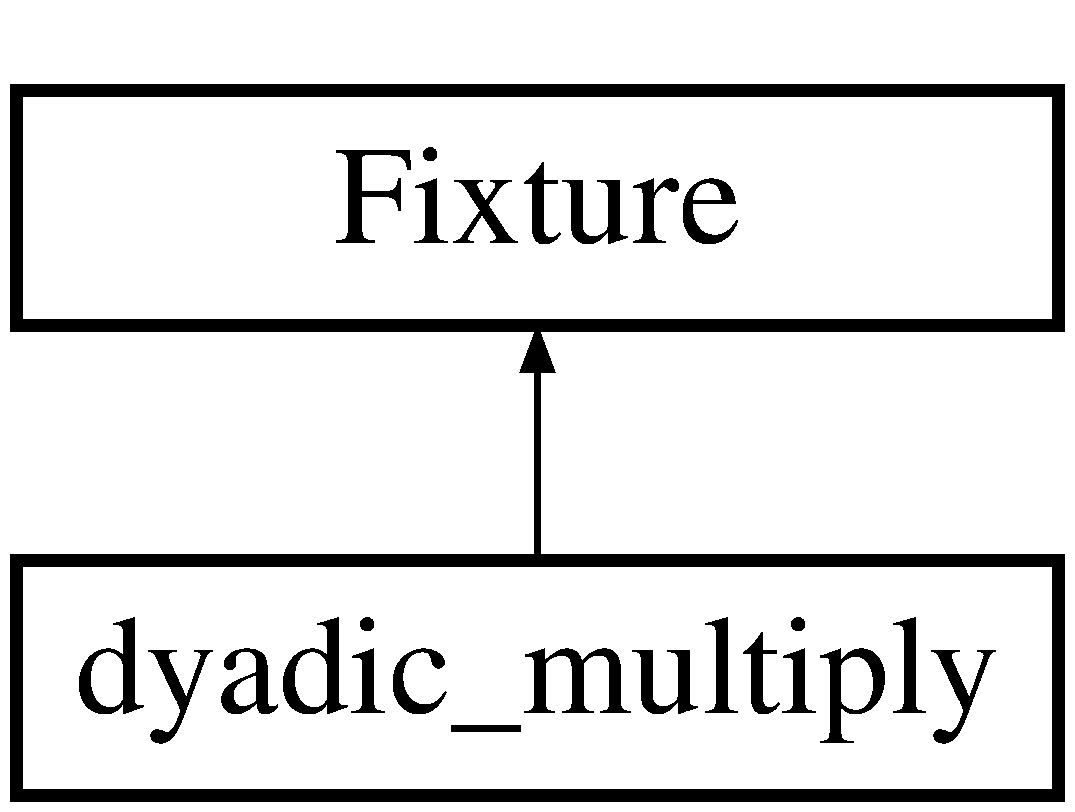
\includegraphics[height=2.000000cm]{classdyadic__multiply}
\end{center}
\end{figure}
\subsection*{Public Member Functions}
\begin{DoxyCompactItemize}
\item 
void \hyperlink{classdyadic__multiply_ae7e70c56054e97f2e7422865401a1d18}{setup\-\_\-dyadic\-\_\-multiply\-\_\-io} (uint64\-\_\-t \hyperlink{bench__dyadic__multiply_8cpp_a1249f7c009d650067cdc1e2254fcb63c}{n\-\_\-dyadic\-\_\-multiply}, uint64\-\_\-t \hyperlink{bench__dyadic__multiply_8cpp_a94cbf59cad79634589387a30784ed78d}{num\-\_\-moduli}, uint64\-\_\-t coeff\-\_\-count)
\item 
void \hyperlink{classdyadic__multiply_a7104e784aa094e223ab692ab3cd1a663}{bench\-\_\-dyadic\-\_\-multiply} (std\-::vector$<$ uint64\-\_\-t $>$ \&\hyperlink{bench__dyadic__multiply_8cpp_a9df79bfc3d20b59bcaf8d6721d1b8b82}{out}, uint64\-\_\-t \hyperlink{bench__dyadic__multiply_8cpp_a1249f7c009d650067cdc1e2254fcb63c}{n\-\_\-dyadic\-\_\-multiply}, uint64\-\_\-t \hyperlink{bench__dyadic__multiply_8cpp_a94cbf59cad79634589387a30784ed78d}{num\-\_\-moduli}, uint64\-\_\-t coeff\-\_\-count)
\end{DoxyCompactItemize}


\subsection{Member Function Documentation}
\hypertarget{classdyadic__multiply_a7104e784aa094e223ab692ab3cd1a663}{\index{dyadic\-\_\-multiply@{dyadic\-\_\-multiply}!bench\-\_\-dyadic\-\_\-multiply@{bench\-\_\-dyadic\-\_\-multiply}}
\index{bench\-\_\-dyadic\-\_\-multiply@{bench\-\_\-dyadic\-\_\-multiply}!dyadic_multiply@{dyadic\-\_\-multiply}}
\subsubsection[{bench\-\_\-dyadic\-\_\-multiply}]{\setlength{\rightskip}{0pt plus 5cm}void dyadic\-\_\-multiply\-::bench\-\_\-dyadic\-\_\-multiply (
\begin{DoxyParamCaption}
\item[{std\-::vector$<$ uint64\-\_\-t $>$ \&}]{out, }
\item[{uint64\-\_\-t}]{n\-\_\-dyadic\-\_\-multiply, }
\item[{uint64\-\_\-t}]{num\-\_\-moduli, }
\item[{uint64\-\_\-t}]{coeff\-\_\-count}
\end{DoxyParamCaption}
)}}\label{classdyadic__multiply_a7104e784aa094e223ab692ab3cd1a663}
\hypertarget{classdyadic__multiply_ae7e70c56054e97f2e7422865401a1d18}{\index{dyadic\-\_\-multiply@{dyadic\-\_\-multiply}!setup\-\_\-dyadic\-\_\-multiply\-\_\-io@{setup\-\_\-dyadic\-\_\-multiply\-\_\-io}}
\index{setup\-\_\-dyadic\-\_\-multiply\-\_\-io@{setup\-\_\-dyadic\-\_\-multiply\-\_\-io}!dyadic_multiply@{dyadic\-\_\-multiply}}
\subsubsection[{setup\-\_\-dyadic\-\_\-multiply\-\_\-io}]{\setlength{\rightskip}{0pt plus 5cm}void dyadic\-\_\-multiply\-::setup\-\_\-dyadic\-\_\-multiply\-\_\-io (
\begin{DoxyParamCaption}
\item[{uint64\-\_\-t}]{n\-\_\-dyadic\-\_\-multiply, }
\item[{uint64\-\_\-t}]{num\-\_\-moduli, }
\item[{uint64\-\_\-t}]{coeff\-\_\-count}
\end{DoxyParamCaption}
)}}\label{classdyadic__multiply_ae7e70c56054e97f2e7422865401a1d18}


The documentation for this class was generated from the following file\-:\begin{DoxyCompactItemize}
\item 
\hyperlink{bench__dyadic__multiply_8cpp}{bench\-\_\-dyadic\-\_\-multiply.\-cpp}\end{DoxyCompactItemize}

\hypertarget{classdyadic__multiply__test}{\section{dyadic\-\_\-multiply\-\_\-test Class Reference}
\label{classdyadic__multiply__test}\index{dyadic\-\_\-multiply\-\_\-test@{dyadic\-\_\-multiply\-\_\-test}}
}
Inheritance diagram for dyadic\-\_\-multiply\-\_\-test\-:\begin{figure}[H]
\begin{center}
\leavevmode
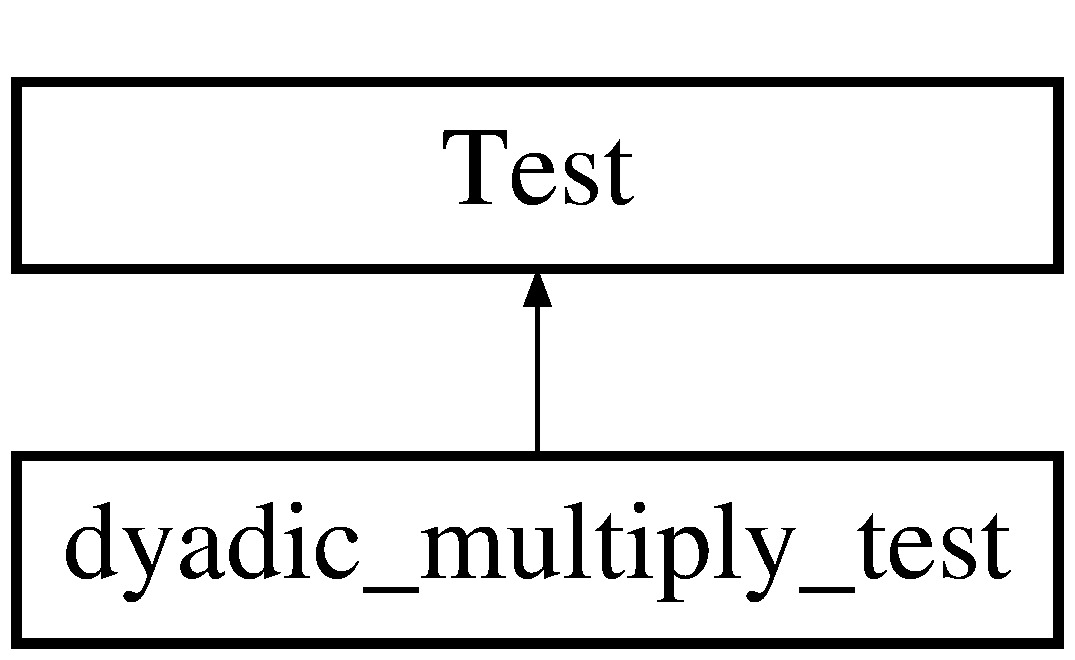
\includegraphics[height=2.000000cm]{classdyadic__multiply__test}
\end{center}
\end{figure}
\subsection*{Public Member Functions}
\begin{DoxyCompactItemize}
\item 
void \hyperlink{classdyadic__multiply__test_a30c5897858c8434401ae46efc05d53b0}{test\-\_\-dyadic\-\_\-multiply} (uint64\-\_\-t num\-\_\-dyadic\-\_\-multiply, uint64\-\_\-t num\-\_\-moduli, uint64\-\_\-t coeff\-\_\-count, bool death=false)
\item 
void \hyperlink{classdyadic__multiply__test_aed73bb19b0e21ab956ee635db8e783c3}{test\-\_\-matrix\-\_\-dyadic\-\_\-multiply} (uint64\-\_\-t n\-\_\-rows, uint64\-\_\-t n\-\_\-columns, uint64\-\_\-t num\-\_\-moduli, uint64\-\_\-t coeff\-\_\-count)
\item 
void \hyperlink{classdyadic__multiply__test_a4f423f1c9b8b1821ce865b53488708a3}{Test\-Body} () override
\end{DoxyCompactItemize}


\subsection{Member Function Documentation}
\hypertarget{classdyadic__multiply__test_a30c5897858c8434401ae46efc05d53b0}{\index{dyadic\-\_\-multiply\-\_\-test@{dyadic\-\_\-multiply\-\_\-test}!test\-\_\-dyadic\-\_\-multiply@{test\-\_\-dyadic\-\_\-multiply}}
\index{test\-\_\-dyadic\-\_\-multiply@{test\-\_\-dyadic\-\_\-multiply}!dyadic_multiply_test@{dyadic\-\_\-multiply\-\_\-test}}
\subsubsection[{test\-\_\-dyadic\-\_\-multiply}]{\setlength{\rightskip}{0pt plus 5cm}void dyadic\-\_\-multiply\-\_\-test\-::test\-\_\-dyadic\-\_\-multiply (
\begin{DoxyParamCaption}
\item[{uint64\-\_\-t}]{num\-\_\-dyadic\-\_\-multiply, }
\item[{uint64\-\_\-t}]{num\-\_\-moduli, }
\item[{uint64\-\_\-t}]{coeff\-\_\-count, }
\item[{bool}]{death = {\ttfamily false}}
\end{DoxyParamCaption}
)}}\label{classdyadic__multiply__test_a30c5897858c8434401ae46efc05d53b0}
\hypertarget{classdyadic__multiply__test_aed73bb19b0e21ab956ee635db8e783c3}{\index{dyadic\-\_\-multiply\-\_\-test@{dyadic\-\_\-multiply\-\_\-test}!test\-\_\-matrix\-\_\-dyadic\-\_\-multiply@{test\-\_\-matrix\-\_\-dyadic\-\_\-multiply}}
\index{test\-\_\-matrix\-\_\-dyadic\-\_\-multiply@{test\-\_\-matrix\-\_\-dyadic\-\_\-multiply}!dyadic_multiply_test@{dyadic\-\_\-multiply\-\_\-test}}
\subsubsection[{test\-\_\-matrix\-\_\-dyadic\-\_\-multiply}]{\setlength{\rightskip}{0pt plus 5cm}void dyadic\-\_\-multiply\-\_\-test\-::test\-\_\-matrix\-\_\-dyadic\-\_\-multiply (
\begin{DoxyParamCaption}
\item[{uint64\-\_\-t}]{n\-\_\-rows, }
\item[{uint64\-\_\-t}]{n\-\_\-columns, }
\item[{uint64\-\_\-t}]{num\-\_\-moduli, }
\item[{uint64\-\_\-t}]{coeff\-\_\-count}
\end{DoxyParamCaption}
)}}\label{classdyadic__multiply__test_aed73bb19b0e21ab956ee635db8e783c3}
\hypertarget{classdyadic__multiply__test_a4f423f1c9b8b1821ce865b53488708a3}{\index{dyadic\-\_\-multiply\-\_\-test@{dyadic\-\_\-multiply\-\_\-test}!Test\-Body@{Test\-Body}}
\index{Test\-Body@{Test\-Body}!dyadic_multiply_test@{dyadic\-\_\-multiply\-\_\-test}}
\subsubsection[{Test\-Body}]{\setlength{\rightskip}{0pt plus 5cm}void dyadic\-\_\-multiply\-\_\-test\-::\-Test\-Body (
\begin{DoxyParamCaption}
{}
\end{DoxyParamCaption}
)\hspace{0.3cm}{\ttfamily [inline]}, {\ttfamily [override]}}}\label{classdyadic__multiply__test_a4f423f1c9b8b1821ce865b53488708a3}


The documentation for this class was generated from the following file\-:\begin{DoxyCompactItemize}
\item 
\hyperlink{test__dyadic__multiply_8cpp}{test\-\_\-dyadic\-\_\-multiply.\-cpp}\end{DoxyCompactItemize}

\hypertarget{classexample__dyadic__multiply}{\section{example\-\_\-dyadic\-\_\-multiply Class Reference}
\label{classexample__dyadic__multiply}\index{example\-\_\-dyadic\-\_\-multiply@{example\-\_\-dyadic\-\_\-multiply}}
}


{\ttfamily \#include $<$example\-\_\-dyadic\-\_\-multiply.\-h$>$}

\subsection*{Public Member Functions}
\begin{DoxyCompactItemize}
\item 
void \hyperlink{classexample__dyadic__multiply_a0816be553ba8877e38dd37edf5d166be}{setup\-\_\-dyadic\-\_\-multiply} (uint64\-\_\-t \hyperlink{bench__dyadic__multiply_8cpp_a1249f7c009d650067cdc1e2254fcb63c}{n\-\_\-dyadic\-\_\-multiply}, uint64\-\_\-t \hyperlink{bench__dyadic__multiply_8cpp_a94cbf59cad79634589387a30784ed78d}{num\-\_\-moduli}, uint64\-\_\-t coeff\-\_\-count)
\begin{DoxyCompactList}\small\item\em \hyperlink{classexample__dyadic__multiply_a0816be553ba8877e38dd37edf5d166be}{example\-\_\-dyadic\-\_\-multiply\-::setup\-\_\-dyadic\-\_\-multiply} Initializes the multiplication two operands and the vector of moduli Compute and stores the expected multiplication result for future validation. \end{DoxyCompactList}\item 
void \hyperlink{classexample__dyadic__multiply_a1f21e56107b4fc4f522fd59ecc0f3697}{execute\-\_\-dyadic\-\_\-multiply} (std\-::vector$<$ uint64\-\_\-t $>$ \&\hyperlink{bench__dyadic__multiply_8cpp_a9df79bfc3d20b59bcaf8d6721d1b8b82}{out}, uint64\-\_\-t \hyperlink{bench__dyadic__multiply_8cpp_a1249f7c009d650067cdc1e2254fcb63c}{n\-\_\-dyadic\-\_\-multiply}, uint64\-\_\-t \hyperlink{bench__dyadic__multiply_8cpp_a94cbf59cad79634589387a30784ed78d}{num\-\_\-moduli}, uint64\-\_\-t coeff\-\_\-count)
\begin{DoxyCompactList}\small\item\em \hyperlink{classexample__dyadic__multiply_a1f21e56107b4fc4f522fd59ecc0f3697}{example\-\_\-dyadic\-\_\-multiply\-::execute\-\_\-dyadic\-\_\-multiply} sets the work size for the multiplication calls n\-\_\-dyadic\-\_\-multiply times the multiplication function calls Dyadic\-Multiply\-Completed after completion of all multiplications \end{DoxyCompactList}\item 
std\-::vector$<$ uint64\-\_\-t $>$ \& \hyperlink{classexample__dyadic__multiply_a11ae693700a81cd88fdc75be651f2048}{exp\-\_\-output} ()
\end{DoxyCompactItemize}


\subsection{Member Function Documentation}
\hypertarget{classexample__dyadic__multiply_a1f21e56107b4fc4f522fd59ecc0f3697}{\index{example\-\_\-dyadic\-\_\-multiply@{example\-\_\-dyadic\-\_\-multiply}!execute\-\_\-dyadic\-\_\-multiply@{execute\-\_\-dyadic\-\_\-multiply}}
\index{execute\-\_\-dyadic\-\_\-multiply@{execute\-\_\-dyadic\-\_\-multiply}!example_dyadic_multiply@{example\-\_\-dyadic\-\_\-multiply}}
\subsubsection[{execute\-\_\-dyadic\-\_\-multiply}]{\setlength{\rightskip}{0pt plus 5cm}void example\-\_\-dyadic\-\_\-multiply\-::execute\-\_\-dyadic\-\_\-multiply (
\begin{DoxyParamCaption}
\item[{std\-::vector$<$ uint64\-\_\-t $>$ \&}]{out, }
\item[{uint64\-\_\-t}]{n\-\_\-dyadic\-\_\-multiply, }
\item[{uint64\-\_\-t}]{num\-\_\-moduli, }
\item[{uint64\-\_\-t}]{coeff\-\_\-count}
\end{DoxyParamCaption}
)}}\label{classexample__dyadic__multiply_a1f21e56107b4fc4f522fd59ecc0f3697}


\hyperlink{classexample__dyadic__multiply_a1f21e56107b4fc4f522fd59ecc0f3697}{example\-\_\-dyadic\-\_\-multiply\-::execute\-\_\-dyadic\-\_\-multiply} sets the work size for the multiplication calls n\-\_\-dyadic\-\_\-multiply times the multiplication function calls Dyadic\-Multiply\-Completed after completion of all multiplications 

\hypertarget{classexample__dyadic__multiply_a11ae693700a81cd88fdc75be651f2048}{\index{example\-\_\-dyadic\-\_\-multiply@{example\-\_\-dyadic\-\_\-multiply}!exp\-\_\-output@{exp\-\_\-output}}
\index{exp\-\_\-output@{exp\-\_\-output}!example_dyadic_multiply@{example\-\_\-dyadic\-\_\-multiply}}
\subsubsection[{exp\-\_\-output}]{\setlength{\rightskip}{0pt plus 5cm}std\-::vector$<$uint64\-\_\-t$>$\& example\-\_\-dyadic\-\_\-multiply\-::exp\-\_\-output (
\begin{DoxyParamCaption}
{}
\end{DoxyParamCaption}
)\hspace{0.3cm}{\ttfamily [inline]}}}\label{classexample__dyadic__multiply_a11ae693700a81cd88fdc75be651f2048}
\hypertarget{classexample__dyadic__multiply_a0816be553ba8877e38dd37edf5d166be}{\index{example\-\_\-dyadic\-\_\-multiply@{example\-\_\-dyadic\-\_\-multiply}!setup\-\_\-dyadic\-\_\-multiply@{setup\-\_\-dyadic\-\_\-multiply}}
\index{setup\-\_\-dyadic\-\_\-multiply@{setup\-\_\-dyadic\-\_\-multiply}!example_dyadic_multiply@{example\-\_\-dyadic\-\_\-multiply}}
\subsubsection[{setup\-\_\-dyadic\-\_\-multiply}]{\setlength{\rightskip}{0pt plus 5cm}void example\-\_\-dyadic\-\_\-multiply\-::setup\-\_\-dyadic\-\_\-multiply (
\begin{DoxyParamCaption}
\item[{uint64\-\_\-t}]{n\-\_\-dyadic\-\_\-multiply, }
\item[{uint64\-\_\-t}]{num\-\_\-moduli, }
\item[{uint64\-\_\-t}]{coeff\-\_\-count}
\end{DoxyParamCaption}
)}}\label{classexample__dyadic__multiply_a0816be553ba8877e38dd37edf5d166be}


\hyperlink{classexample__dyadic__multiply_a0816be553ba8877e38dd37edf5d166be}{example\-\_\-dyadic\-\_\-multiply\-::setup\-\_\-dyadic\-\_\-multiply} Initializes the multiplication two operands and the vector of moduli Compute and stores the expected multiplication result for future validation. 



The documentation for this class was generated from the following files\-:\begin{DoxyCompactItemize}
\item 
\hyperlink{example__dyadic__multiply_8h}{example\-\_\-dyadic\-\_\-multiply.\-h}\item 
\hyperlink{example__dyadic__multiply_8cpp}{example\-\_\-dyadic\-\_\-multiply.\-cpp}\end{DoxyCompactItemize}

\hypertarget{classfpga__context}{\section{fpga\-\_\-context Class Reference}
\label{classfpga__context}\index{fpga\-\_\-context@{fpga\-\_\-context}}
}


{\ttfamily \#include $<$fpga\-\_\-context.\-h$>$}

Inheritance diagram for fpga\-\_\-context\-:\begin{figure}[H]
\begin{center}
\leavevmode
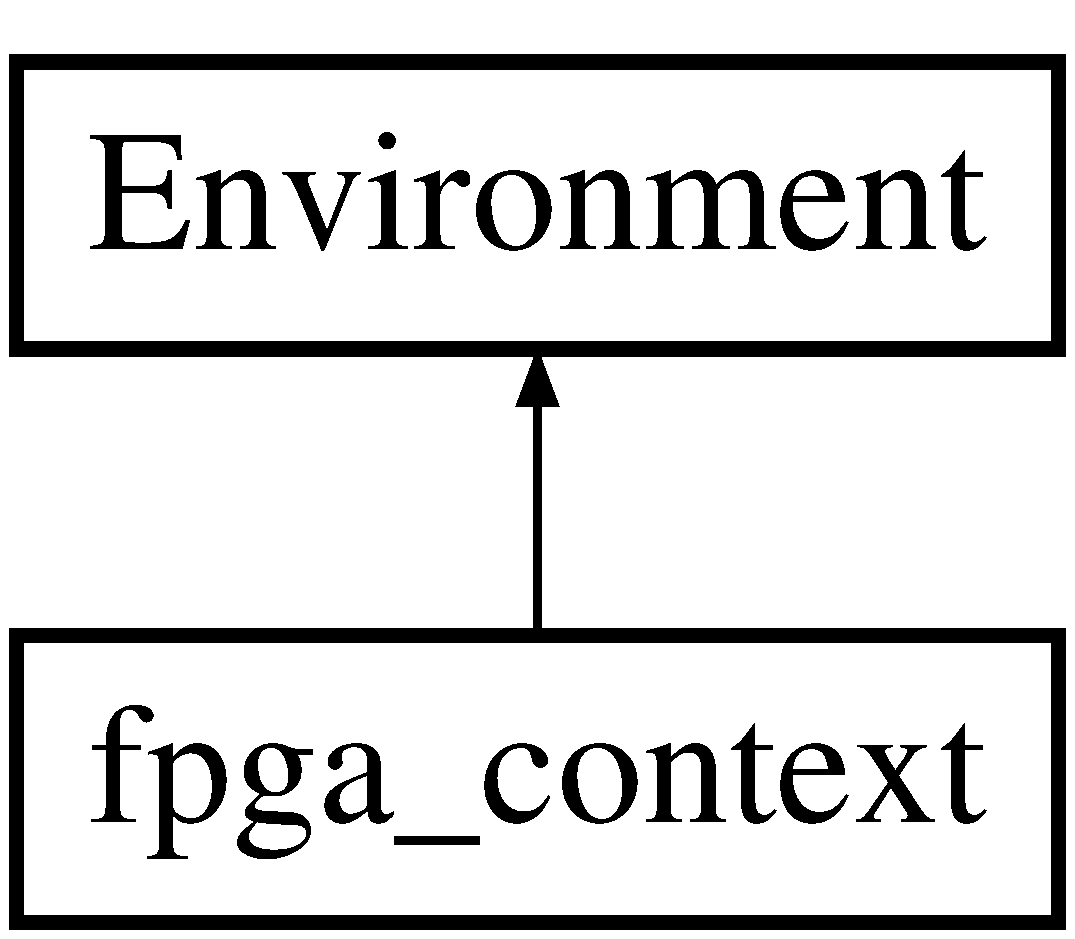
\includegraphics[height=2.000000cm]{classfpga__context}
\end{center}
\end{figure}
\subsection*{Public Member Functions}
\begin{DoxyCompactItemize}
\item 
virtual \hyperlink{classfpga__context_a1bb9192ffc2972fe6ee6deb85bec921e}{$\sim$fpga\-\_\-context} ()
\item 
virtual void \hyperlink{classfpga__context_a8650400eca53431dd95795429c484624}{Set\-Up} ()
\item 
virtual void \hyperlink{classfpga__context_a3f229df43f9dff43cd2f748b72023e2a}{Tear\-Down} ()
\end{DoxyCompactItemize}


\subsection{Constructor \& Destructor Documentation}
\hypertarget{classfpga__context_a1bb9192ffc2972fe6ee6deb85bec921e}{\index{fpga\-\_\-context@{fpga\-\_\-context}!$\sim$fpga\-\_\-context@{$\sim$fpga\-\_\-context}}
\index{$\sim$fpga\-\_\-context@{$\sim$fpga\-\_\-context}!fpga_context@{fpga\-\_\-context}}
\subsubsection[{$\sim$fpga\-\_\-context}]{\setlength{\rightskip}{0pt plus 5cm}virtual fpga\-\_\-context\-::$\sim$fpga\-\_\-context (
\begin{DoxyParamCaption}
{}
\end{DoxyParamCaption}
)\hspace{0.3cm}{\ttfamily [inline]}, {\ttfamily [virtual]}}}\label{classfpga__context_a1bb9192ffc2972fe6ee6deb85bec921e}


\subsection{Member Function Documentation}
\hypertarget{classfpga__context_a8650400eca53431dd95795429c484624}{\index{fpga\-\_\-context@{fpga\-\_\-context}!Set\-Up@{Set\-Up}}
\index{Set\-Up@{Set\-Up}!fpga_context@{fpga\-\_\-context}}
\subsubsection[{Set\-Up}]{\setlength{\rightskip}{0pt plus 5cm}virtual void fpga\-\_\-context\-::\-Set\-Up (
\begin{DoxyParamCaption}
{}
\end{DoxyParamCaption}
)\hspace{0.3cm}{\ttfamily [inline]}, {\ttfamily [virtual]}}}\label{classfpga__context_a8650400eca53431dd95795429c484624}
\hypertarget{classfpga__context_a3f229df43f9dff43cd2f748b72023e2a}{\index{fpga\-\_\-context@{fpga\-\_\-context}!Tear\-Down@{Tear\-Down}}
\index{Tear\-Down@{Tear\-Down}!fpga_context@{fpga\-\_\-context}}
\subsubsection[{Tear\-Down}]{\setlength{\rightskip}{0pt plus 5cm}virtual void fpga\-\_\-context\-::\-Tear\-Down (
\begin{DoxyParamCaption}
{}
\end{DoxyParamCaption}
)\hspace{0.3cm}{\ttfamily [inline]}, {\ttfamily [virtual]}}}\label{classfpga__context_a3f229df43f9dff43cd2f748b72023e2a}


The documentation for this class was generated from the following file\-:\begin{DoxyCompactItemize}
\item 
\hyperlink{tests_2fpga__context_8h}{tests/fpga\-\_\-context.\-h}\end{DoxyCompactItemize}

\hypertarget{structintel_1_1hexl_1_1fpga_1_1FPGAObject}{\section{intel\-:\-:hexl\-:\-:fpga\-:\-:F\-P\-G\-A\-Object Struct Reference}
\label{structintel_1_1hexl_1_1fpga_1_1FPGAObject}\index{intel\-::hexl\-::fpga\-::\-F\-P\-G\-A\-Object@{intel\-::hexl\-::fpga\-::\-F\-P\-G\-A\-Object}}
}


Parent Struct \hyperlink{structintel_1_1hexl_1_1fpga_1_1FPGAObject}{F\-P\-G\-A\-Object} stores the blob of objects to be transfered to the F\-P\-G\-A.  




{\ttfamily \#include $<$fpga.\-h$>$}

Inheritance diagram for intel\-:\-:hexl\-:\-:fpga\-:\-:F\-P\-G\-A\-Object\-:\begin{figure}[H]
\begin{center}
\leavevmode
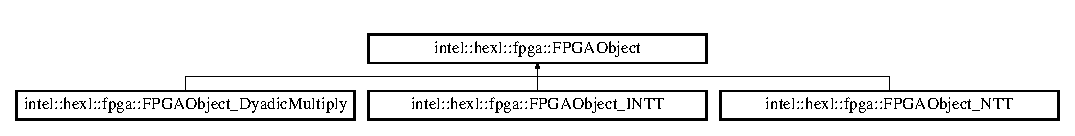
\includegraphics[height=1.377614cm]{structintel_1_1hexl_1_1fpga_1_1FPGAObject}
\end{center}
\end{figure}
\subsection*{Public Member Functions}
\begin{DoxyCompactItemize}
\item 
\hyperlink{structintel_1_1hexl_1_1fpga_1_1FPGAObject_a1b07c859e7c9205ac12cdb7cd0ba61f7}{F\-P\-G\-A\-Object} (const cl\-\_\-context \&context, uint64\-\_\-t n\-\_\-batch)
\item 
virtual \hyperlink{structintel_1_1hexl_1_1fpga_1_1FPGAObject_adecdea2bd81579b973e9292045c8d400}{$\sim$\-F\-P\-G\-A\-Object} ()=default
\item 
virtual void \hyperlink{structintel_1_1hexl_1_1fpga_1_1FPGAObject_abd665113bfb3b0e7a33e09078f01ae43}{fill\-\_\-in\-\_\-data} (const std\-::vector$<$ \hyperlink{structintel_1_1hexl_1_1fpga_1_1Object}{Object} $\ast$ $>$ \&objs)=0
\item 
virtual void \hyperlink{structintel_1_1hexl_1_1fpga_1_1FPGAObject_a954c4c75077a7c406f6c81517ea7bb04}{fill\-\_\-out\-\_\-data} (uint64\-\_\-t $\ast$results)=0
\item 
void \hyperlink{structintel_1_1hexl_1_1fpga_1_1FPGAObject_a0131d230161e662b63af86099177beb7}{recycle} ()
\end{DoxyCompactItemize}
\subsection*{Public Attributes}
\begin{DoxyCompactItemize}
\item 
const cl\-\_\-context \& \hyperlink{structintel_1_1hexl_1_1fpga_1_1FPGAObject_a87af81d73a95ab1c31c8cd9ebf4b1bba}{context\-\_\-}
\item 
int \hyperlink{structintel_1_1hexl_1_1fpga_1_1FPGAObject_a246901212706cfac8299f3b47419f33f}{tag\-\_\-}
\item 
uint64\-\_\-t \hyperlink{structintel_1_1hexl_1_1fpga_1_1FPGAObject_a350704607558ab455334aebe055fc2d4}{n\-\_\-batch\-\_\-}
\item 
std\-::vector$<$ \hyperlink{structintel_1_1hexl_1_1fpga_1_1Object}{Object} $\ast$ $>$ \hyperlink{structintel_1_1hexl_1_1fpga_1_1FPGAObject_a51ecca2b08e9e9d67036d8419acca68b}{in\-\_\-objs\-\_\-}
\end{DoxyCompactItemize}
\subsection*{Static Public Attributes}
\begin{DoxyCompactItemize}
\item 
static std\-::atomic$<$ int $>$ \hyperlink{structintel_1_1hexl_1_1fpga_1_1FPGAObject_a99733056751a8574c4573210bb03d5a3}{g\-\_\-tag\-\_\-}
\end{DoxyCompactItemize}


\subsection{Detailed Description}
Parent Struct \hyperlink{structintel_1_1hexl_1_1fpga_1_1FPGAObject}{F\-P\-G\-A\-Object} stores the blob of objects to be transfered to the F\-P\-G\-A. 

fill\-\_\-in\-\_\-data 
\begin{DoxyParams}[1]{Parameters}
\mbox{\tt in}  & {\em vector} & of objects  fill\-\_\-out\-\_\-data \\
\hline
\mbox{\tt out}  & {\em vector} & of results  recycle releases the content context stores the open\-C\-L context tag stores the blob tag n\-\_\-batch stores the number of batches in\-\_\-objs\-\_\- vector of stored objects g\-\_\-tag\-\_\- stores the global tag identifier \\
\hline
\end{DoxyParams}


\subsection{Constructor \& Destructor Documentation}
\hypertarget{structintel_1_1hexl_1_1fpga_1_1FPGAObject_a1b07c859e7c9205ac12cdb7cd0ba61f7}{\index{intel\-::hexl\-::fpga\-::\-F\-P\-G\-A\-Object@{intel\-::hexl\-::fpga\-::\-F\-P\-G\-A\-Object}!F\-P\-G\-A\-Object@{F\-P\-G\-A\-Object}}
\index{F\-P\-G\-A\-Object@{F\-P\-G\-A\-Object}!intel::hexl::fpga::FPGAObject@{intel\-::hexl\-::fpga\-::\-F\-P\-G\-A\-Object}}
\subsubsection[{F\-P\-G\-A\-Object}]{\setlength{\rightskip}{0pt plus 5cm}intel\-::hexl\-::fpga\-::\-F\-P\-G\-A\-Object\-::\-F\-P\-G\-A\-Object (
\begin{DoxyParamCaption}
\item[{const cl\-\_\-context \&}]{context, }
\item[{uint64\-\_\-t}]{n\-\_\-batch}
\end{DoxyParamCaption}
)}}\label{structintel_1_1hexl_1_1fpga_1_1FPGAObject_a1b07c859e7c9205ac12cdb7cd0ba61f7}
\hypertarget{structintel_1_1hexl_1_1fpga_1_1FPGAObject_adecdea2bd81579b973e9292045c8d400}{\index{intel\-::hexl\-::fpga\-::\-F\-P\-G\-A\-Object@{intel\-::hexl\-::fpga\-::\-F\-P\-G\-A\-Object}!$\sim$\-F\-P\-G\-A\-Object@{$\sim$\-F\-P\-G\-A\-Object}}
\index{$\sim$\-F\-P\-G\-A\-Object@{$\sim$\-F\-P\-G\-A\-Object}!intel::hexl::fpga::FPGAObject@{intel\-::hexl\-::fpga\-::\-F\-P\-G\-A\-Object}}
\subsubsection[{$\sim$\-F\-P\-G\-A\-Object}]{\setlength{\rightskip}{0pt plus 5cm}virtual intel\-::hexl\-::fpga\-::\-F\-P\-G\-A\-Object\-::$\sim$\-F\-P\-G\-A\-Object (
\begin{DoxyParamCaption}
{}
\end{DoxyParamCaption}
)\hspace{0.3cm}{\ttfamily [virtual]}, {\ttfamily [default]}}}\label{structintel_1_1hexl_1_1fpga_1_1FPGAObject_adecdea2bd81579b973e9292045c8d400}


\subsection{Member Function Documentation}
\hypertarget{structintel_1_1hexl_1_1fpga_1_1FPGAObject_abd665113bfb3b0e7a33e09078f01ae43}{\index{intel\-::hexl\-::fpga\-::\-F\-P\-G\-A\-Object@{intel\-::hexl\-::fpga\-::\-F\-P\-G\-A\-Object}!fill\-\_\-in\-\_\-data@{fill\-\_\-in\-\_\-data}}
\index{fill\-\_\-in\-\_\-data@{fill\-\_\-in\-\_\-data}!intel::hexl::fpga::FPGAObject@{intel\-::hexl\-::fpga\-::\-F\-P\-G\-A\-Object}}
\subsubsection[{fill\-\_\-in\-\_\-data}]{\setlength{\rightskip}{0pt plus 5cm}virtual void intel\-::hexl\-::fpga\-::\-F\-P\-G\-A\-Object\-::fill\-\_\-in\-\_\-data (
\begin{DoxyParamCaption}
\item[{const std\-::vector$<$ {\bf Object} $\ast$ $>$ \&}]{objs}
\end{DoxyParamCaption}
)\hspace{0.3cm}{\ttfamily [pure virtual]}}}\label{structintel_1_1hexl_1_1fpga_1_1FPGAObject_abd665113bfb3b0e7a33e09078f01ae43}


Implemented in \hyperlink{structintel_1_1hexl_1_1fpga_1_1FPGAObject__DyadicMultiply_aa4f825403efabeffbf3c9eee6cf0ecb1}{intel\-::hexl\-::fpga\-::\-F\-P\-G\-A\-Object\-\_\-\-Dyadic\-Multiply}, \hyperlink{structintel_1_1hexl_1_1fpga_1_1FPGAObject__INTT_a3af9d73a583150a06fee9288a7938e31}{intel\-::hexl\-::fpga\-::\-F\-P\-G\-A\-Object\-\_\-\-I\-N\-T\-T}, and \hyperlink{structintel_1_1hexl_1_1fpga_1_1FPGAObject__NTT_a3aa5e6c85ae154bcf98ba99205feda16}{intel\-::hexl\-::fpga\-::\-F\-P\-G\-A\-Object\-\_\-\-N\-T\-T}.

\hypertarget{structintel_1_1hexl_1_1fpga_1_1FPGAObject_a954c4c75077a7c406f6c81517ea7bb04}{\index{intel\-::hexl\-::fpga\-::\-F\-P\-G\-A\-Object@{intel\-::hexl\-::fpga\-::\-F\-P\-G\-A\-Object}!fill\-\_\-out\-\_\-data@{fill\-\_\-out\-\_\-data}}
\index{fill\-\_\-out\-\_\-data@{fill\-\_\-out\-\_\-data}!intel::hexl::fpga::FPGAObject@{intel\-::hexl\-::fpga\-::\-F\-P\-G\-A\-Object}}
\subsubsection[{fill\-\_\-out\-\_\-data}]{\setlength{\rightskip}{0pt plus 5cm}virtual void intel\-::hexl\-::fpga\-::\-F\-P\-G\-A\-Object\-::fill\-\_\-out\-\_\-data (
\begin{DoxyParamCaption}
\item[{uint64\-\_\-t $\ast$}]{results}
\end{DoxyParamCaption}
)\hspace{0.3cm}{\ttfamily [pure virtual]}}}\label{structintel_1_1hexl_1_1fpga_1_1FPGAObject_a954c4c75077a7c406f6c81517ea7bb04}


Implemented in \hyperlink{structintel_1_1hexl_1_1fpga_1_1FPGAObject__DyadicMultiply_a2a95c53a7a8bcca57da535a5ad6e7692}{intel\-::hexl\-::fpga\-::\-F\-P\-G\-A\-Object\-\_\-\-Dyadic\-Multiply}, \hyperlink{structintel_1_1hexl_1_1fpga_1_1FPGAObject__INTT_a18c10384468f7e39f15b2059fe59d5db}{intel\-::hexl\-::fpga\-::\-F\-P\-G\-A\-Object\-\_\-\-I\-N\-T\-T}, and \hyperlink{structintel_1_1hexl_1_1fpga_1_1FPGAObject__NTT_a4f31676fdaf820560f625d2f468da397}{intel\-::hexl\-::fpga\-::\-F\-P\-G\-A\-Object\-\_\-\-N\-T\-T}.

\hypertarget{structintel_1_1hexl_1_1fpga_1_1FPGAObject_a0131d230161e662b63af86099177beb7}{\index{intel\-::hexl\-::fpga\-::\-F\-P\-G\-A\-Object@{intel\-::hexl\-::fpga\-::\-F\-P\-G\-A\-Object}!recycle@{recycle}}
\index{recycle@{recycle}!intel::hexl::fpga::FPGAObject@{intel\-::hexl\-::fpga\-::\-F\-P\-G\-A\-Object}}
\subsubsection[{recycle}]{\setlength{\rightskip}{0pt plus 5cm}void intel\-::hexl\-::fpga\-::\-F\-P\-G\-A\-Object\-::recycle (
\begin{DoxyParamCaption}
{}
\end{DoxyParamCaption}
)}}\label{structintel_1_1hexl_1_1fpga_1_1FPGAObject_a0131d230161e662b63af86099177beb7}


\subsection{Member Data Documentation}
\hypertarget{structintel_1_1hexl_1_1fpga_1_1FPGAObject_a87af81d73a95ab1c31c8cd9ebf4b1bba}{\index{intel\-::hexl\-::fpga\-::\-F\-P\-G\-A\-Object@{intel\-::hexl\-::fpga\-::\-F\-P\-G\-A\-Object}!context\-\_\-@{context\-\_\-}}
\index{context\-\_\-@{context\-\_\-}!intel::hexl::fpga::FPGAObject@{intel\-::hexl\-::fpga\-::\-F\-P\-G\-A\-Object}}
\subsubsection[{context\-\_\-}]{\setlength{\rightskip}{0pt plus 5cm}const cl\-\_\-context\& intel\-::hexl\-::fpga\-::\-F\-P\-G\-A\-Object\-::context\-\_\-}}\label{structintel_1_1hexl_1_1fpga_1_1FPGAObject_a87af81d73a95ab1c31c8cd9ebf4b1bba}
\hypertarget{structintel_1_1hexl_1_1fpga_1_1FPGAObject_a99733056751a8574c4573210bb03d5a3}{\index{intel\-::hexl\-::fpga\-::\-F\-P\-G\-A\-Object@{intel\-::hexl\-::fpga\-::\-F\-P\-G\-A\-Object}!g\-\_\-tag\-\_\-@{g\-\_\-tag\-\_\-}}
\index{g\-\_\-tag\-\_\-@{g\-\_\-tag\-\_\-}!intel::hexl::fpga::FPGAObject@{intel\-::hexl\-::fpga\-::\-F\-P\-G\-A\-Object}}
\subsubsection[{g\-\_\-tag\-\_\-}]{\setlength{\rightskip}{0pt plus 5cm}std\-::atomic$<$int$>$ intel\-::hexl\-::fpga\-::\-F\-P\-G\-A\-Object\-::g\-\_\-tag\-\_\-\hspace{0.3cm}{\ttfamily [static]}}}\label{structintel_1_1hexl_1_1fpga_1_1FPGAObject_a99733056751a8574c4573210bb03d5a3}
\hypertarget{structintel_1_1hexl_1_1fpga_1_1FPGAObject_a51ecca2b08e9e9d67036d8419acca68b}{\index{intel\-::hexl\-::fpga\-::\-F\-P\-G\-A\-Object@{intel\-::hexl\-::fpga\-::\-F\-P\-G\-A\-Object}!in\-\_\-objs\-\_\-@{in\-\_\-objs\-\_\-}}
\index{in\-\_\-objs\-\_\-@{in\-\_\-objs\-\_\-}!intel::hexl::fpga::FPGAObject@{intel\-::hexl\-::fpga\-::\-F\-P\-G\-A\-Object}}
\subsubsection[{in\-\_\-objs\-\_\-}]{\setlength{\rightskip}{0pt plus 5cm}std\-::vector$<${\bf Object}$\ast$$>$ intel\-::hexl\-::fpga\-::\-F\-P\-G\-A\-Object\-::in\-\_\-objs\-\_\-}}\label{structintel_1_1hexl_1_1fpga_1_1FPGAObject_a51ecca2b08e9e9d67036d8419acca68b}
\hypertarget{structintel_1_1hexl_1_1fpga_1_1FPGAObject_a350704607558ab455334aebe055fc2d4}{\index{intel\-::hexl\-::fpga\-::\-F\-P\-G\-A\-Object@{intel\-::hexl\-::fpga\-::\-F\-P\-G\-A\-Object}!n\-\_\-batch\-\_\-@{n\-\_\-batch\-\_\-}}
\index{n\-\_\-batch\-\_\-@{n\-\_\-batch\-\_\-}!intel::hexl::fpga::FPGAObject@{intel\-::hexl\-::fpga\-::\-F\-P\-G\-A\-Object}}
\subsubsection[{n\-\_\-batch\-\_\-}]{\setlength{\rightskip}{0pt plus 5cm}uint64\-\_\-t intel\-::hexl\-::fpga\-::\-F\-P\-G\-A\-Object\-::n\-\_\-batch\-\_\-}}\label{structintel_1_1hexl_1_1fpga_1_1FPGAObject_a350704607558ab455334aebe055fc2d4}
\hypertarget{structintel_1_1hexl_1_1fpga_1_1FPGAObject_a246901212706cfac8299f3b47419f33f}{\index{intel\-::hexl\-::fpga\-::\-F\-P\-G\-A\-Object@{intel\-::hexl\-::fpga\-::\-F\-P\-G\-A\-Object}!tag\-\_\-@{tag\-\_\-}}
\index{tag\-\_\-@{tag\-\_\-}!intel::hexl::fpga::FPGAObject@{intel\-::hexl\-::fpga\-::\-F\-P\-G\-A\-Object}}
\subsubsection[{tag\-\_\-}]{\setlength{\rightskip}{0pt plus 5cm}int intel\-::hexl\-::fpga\-::\-F\-P\-G\-A\-Object\-::tag\-\_\-}}\label{structintel_1_1hexl_1_1fpga_1_1FPGAObject_a246901212706cfac8299f3b47419f33f}


The documentation for this struct was generated from the following file\-:\begin{DoxyCompactItemize}
\item 
\hyperlink{fpga_8h}{fpga.\-h}\end{DoxyCompactItemize}

\hypertarget{structintel_1_1hexl_1_1fpga_1_1FPGAObject__DyadicMultiply}{\section{intel\-:\-:hexl\-:\-:fpga\-:\-:F\-P\-G\-A\-Object\-\_\-\-Dyadic\-Multiply Struct Reference}
\label{structintel_1_1hexl_1_1fpga_1_1FPGAObject__DyadicMultiply}\index{intel\-::hexl\-::fpga\-::\-F\-P\-G\-A\-Object\-\_\-\-Dyadic\-Multiply@{intel\-::hexl\-::fpga\-::\-F\-P\-G\-A\-Object\-\_\-\-Dyadic\-Multiply}}
}


Struct \hyperlink{structintel_1_1hexl_1_1fpga_1_1FPGAObject__DyadicMultiply}{F\-P\-G\-A\-Object\-\_\-\-Dyadic\-Multiply} Stores the multiplication blob of objects to be transfered to the F\-P\-G\-A.  




{\ttfamily \#include $<$fpga.\-h$>$}

Inheritance diagram for intel\-:\-:hexl\-:\-:fpga\-:\-:F\-P\-G\-A\-Object\-\_\-\-Dyadic\-Multiply\-:\begin{figure}[H]
\begin{center}
\leavevmode
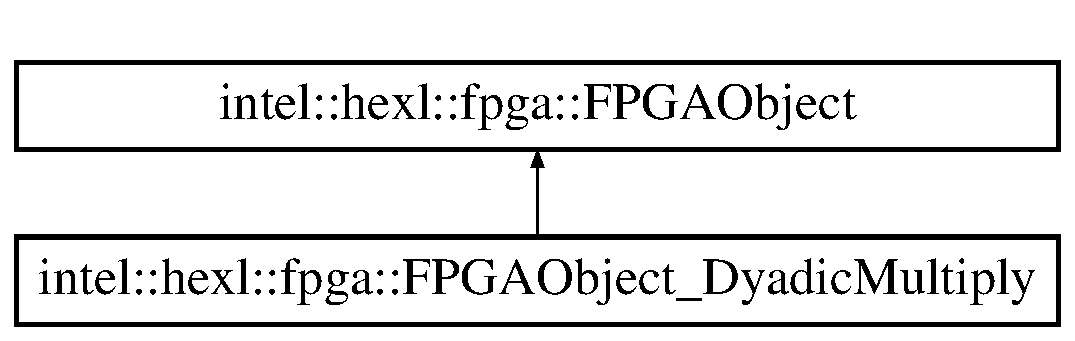
\includegraphics[height=2.000000cm]{structintel_1_1hexl_1_1fpga_1_1FPGAObject__DyadicMultiply}
\end{center}
\end{figure}
\subsection*{Public Member Functions}
\begin{DoxyCompactItemize}
\item 
\hyperlink{structintel_1_1hexl_1_1fpga_1_1FPGAObject__DyadicMultiply_a2246da0a69a18053fe76d8d5b07a3b14}{F\-P\-G\-A\-Object\-\_\-\-Dyadic\-Multiply} (const cl\-\_\-context \&context, uint64\-\_\-t coeff\-\_\-size, uint32\-\_\-t modulus\-\_\-size, uint64\-\_\-t batch\-\_\-size)
\item 
\hyperlink{structintel_1_1hexl_1_1fpga_1_1FPGAObject__DyadicMultiply_adba71553a77b8e2dea74e6c33fde39f5}{$\sim$\-F\-P\-G\-A\-Object\-\_\-\-Dyadic\-Multiply} ()
\item 
\hyperlink{structintel_1_1hexl_1_1fpga_1_1FPGAObject__DyadicMultiply_ab107ff5c684b94d5416d184f6e308f9b}{F\-P\-G\-A\-Object\-\_\-\-Dyadic\-Multiply} (const \hyperlink{structintel_1_1hexl_1_1fpga_1_1FPGAObject__DyadicMultiply}{F\-P\-G\-A\-Object\-\_\-\-Dyadic\-Multiply} \&)=delete
\item 
\hyperlink{structintel_1_1hexl_1_1fpga_1_1FPGAObject__DyadicMultiply}{F\-P\-G\-A\-Object\-\_\-\-Dyadic\-Multiply} \& \hyperlink{structintel_1_1hexl_1_1fpga_1_1FPGAObject__DyadicMultiply_a1be9ab40f69d59dd1c12e9f2ef41b334}{operator=} (const \hyperlink{structintel_1_1hexl_1_1fpga_1_1FPGAObject__DyadicMultiply}{F\-P\-G\-A\-Object\-\_\-\-Dyadic\-Multiply} \&)=delete
\item 
void \hyperlink{structintel_1_1hexl_1_1fpga_1_1FPGAObject__DyadicMultiply_aa4f825403efabeffbf3c9eee6cf0ecb1}{fill\-\_\-in\-\_\-data} (const std\-::vector$<$ \hyperlink{structintel_1_1hexl_1_1fpga_1_1Object}{Object} $\ast$ $>$ \&objs) override
\item 
void \hyperlink{structintel_1_1hexl_1_1fpga_1_1FPGAObject__DyadicMultiply_a2a95c53a7a8bcca57da535a5ad6e7692}{fill\-\_\-out\-\_\-data} (uint64\-\_\-t $\ast$results) override
\end{DoxyCompactItemize}
\subsection*{Public Attributes}
\begin{DoxyCompactItemize}
\item 
uint64\-\_\-t $\ast$ \hyperlink{structintel_1_1hexl_1_1fpga_1_1FPGAObject__DyadicMultiply_a0b6fe933fcb78eefa5296400044bfb72}{operand1\-\_\-in\-\_\-svm\-\_\-}
\item 
uint64\-\_\-t $\ast$ \hyperlink{structintel_1_1hexl_1_1fpga_1_1FPGAObject__DyadicMultiply_a9ea681f4c0135059114239ee3159fe7c}{operand2\-\_\-in\-\_\-svm\-\_\-}
\item 
\hyperlink{structintel_1_1hexl_1_1fpga_1_1moduli__info__t}{moduli\-\_\-info\-\_\-t} $\ast$ \hyperlink{structintel_1_1hexl_1_1fpga_1_1FPGAObject__DyadicMultiply_a4e248c4090cb01ca4f4a4a927f3a5ee0}{moduli\-\_\-info\-\_\-}
\item 
uint64\-\_\-t \hyperlink{structintel_1_1hexl_1_1fpga_1_1FPGAObject__DyadicMultiply_addc32ca18fbc7359effd95d67a50c561}{n\-\_\-}
\item 
uint64\-\_\-t \hyperlink{structintel_1_1hexl_1_1fpga_1_1FPGAObject__DyadicMultiply_a1050f5eda0ca0d101a44ba609a1cfed7}{n\-\_\-moduli\-\_\-}
\item 
cl\-\_\-mem \hyperlink{structintel_1_1hexl_1_1fpga_1_1FPGAObject__DyadicMultiply_a1a0d9e75b852a481bc7c6676854b3bcc}{operands\-\_\-in\-\_\-ddr\-\_\-}
\item 
cl\-\_\-mem \hyperlink{structintel_1_1hexl_1_1fpga_1_1FPGAObject__DyadicMultiply_a5e4758ba8ce2f59c59c214783b85c9c4}{results\-\_\-out\-\_\-ddr\-\_\-}
\end{DoxyCompactItemize}
\subsection*{Additional Inherited Members}


\subsection{Detailed Description}
Struct \hyperlink{structintel_1_1hexl_1_1fpga_1_1FPGAObject__DyadicMultiply}{F\-P\-G\-A\-Object\-\_\-\-Dyadic\-Multiply} Stores the multiplication blob of objects to be transfered to the F\-P\-G\-A. 

fill\-\_\-in\-\_\-data 
\begin{DoxyParams}[1]{Parameters}
\mbox{\tt in}  & {\em vector} & of objects  fill\-\_\-out\-\_\-data \\
\hline
 & {\em results} & vector containing the result of the multiplication\\
\hline
\end{DoxyParams}
operand1\-\_\-in\-\_\-svm\-\_\- First operand for the multiplication operand2\-\_\-in\-\_\-svm\-\_\- Second operand for the multiplication moduli\-\_\-info\-\_\- structure containing information about the moduli n\-\_\- polynomial size n\-\_\-moduli number of moduli operands\-\_\-in\-\_\-ddr\-\_\- pointer to operands in D\-D\-R memory results\-\_\-out\-\_\-ddr\-\_\- pointer to multiplication results in D\-D\-R 

\subsection{Constructor \& Destructor Documentation}
\hypertarget{structintel_1_1hexl_1_1fpga_1_1FPGAObject__DyadicMultiply_a2246da0a69a18053fe76d8d5b07a3b14}{\index{intel\-::hexl\-::fpga\-::\-F\-P\-G\-A\-Object\-\_\-\-Dyadic\-Multiply@{intel\-::hexl\-::fpga\-::\-F\-P\-G\-A\-Object\-\_\-\-Dyadic\-Multiply}!F\-P\-G\-A\-Object\-\_\-\-Dyadic\-Multiply@{F\-P\-G\-A\-Object\-\_\-\-Dyadic\-Multiply}}
\index{F\-P\-G\-A\-Object\-\_\-\-Dyadic\-Multiply@{F\-P\-G\-A\-Object\-\_\-\-Dyadic\-Multiply}!intel::hexl::fpga::FPGAObject_DyadicMultiply@{intel\-::hexl\-::fpga\-::\-F\-P\-G\-A\-Object\-\_\-\-Dyadic\-Multiply}}
\subsubsection[{F\-P\-G\-A\-Object\-\_\-\-Dyadic\-Multiply}]{\setlength{\rightskip}{0pt plus 5cm}intel\-::hexl\-::fpga\-::\-F\-P\-G\-A\-Object\-\_\-\-Dyadic\-Multiply\-::\-F\-P\-G\-A\-Object\-\_\-\-Dyadic\-Multiply (
\begin{DoxyParamCaption}
\item[{const cl\-\_\-context \&}]{context, }
\item[{uint64\-\_\-t}]{coeff\-\_\-size, }
\item[{uint32\-\_\-t}]{modulus\-\_\-size, }
\item[{uint64\-\_\-t}]{batch\-\_\-size}
\end{DoxyParamCaption}
)\hspace{0.3cm}{\ttfamily [explicit]}}}\label{structintel_1_1hexl_1_1fpga_1_1FPGAObject__DyadicMultiply_a2246da0a69a18053fe76d8d5b07a3b14}
\hypertarget{structintel_1_1hexl_1_1fpga_1_1FPGAObject__DyadicMultiply_adba71553a77b8e2dea74e6c33fde39f5}{\index{intel\-::hexl\-::fpga\-::\-F\-P\-G\-A\-Object\-\_\-\-Dyadic\-Multiply@{intel\-::hexl\-::fpga\-::\-F\-P\-G\-A\-Object\-\_\-\-Dyadic\-Multiply}!$\sim$\-F\-P\-G\-A\-Object\-\_\-\-Dyadic\-Multiply@{$\sim$\-F\-P\-G\-A\-Object\-\_\-\-Dyadic\-Multiply}}
\index{$\sim$\-F\-P\-G\-A\-Object\-\_\-\-Dyadic\-Multiply@{$\sim$\-F\-P\-G\-A\-Object\-\_\-\-Dyadic\-Multiply}!intel::hexl::fpga::FPGAObject_DyadicMultiply@{intel\-::hexl\-::fpga\-::\-F\-P\-G\-A\-Object\-\_\-\-Dyadic\-Multiply}}
\subsubsection[{$\sim$\-F\-P\-G\-A\-Object\-\_\-\-Dyadic\-Multiply}]{\setlength{\rightskip}{0pt plus 5cm}intel\-::hexl\-::fpga\-::\-F\-P\-G\-A\-Object\-\_\-\-Dyadic\-Multiply\-::$\sim$\-F\-P\-G\-A\-Object\-\_\-\-Dyadic\-Multiply (
\begin{DoxyParamCaption}
{}
\end{DoxyParamCaption}
)}}\label{structintel_1_1hexl_1_1fpga_1_1FPGAObject__DyadicMultiply_adba71553a77b8e2dea74e6c33fde39f5}
\hypertarget{structintel_1_1hexl_1_1fpga_1_1FPGAObject__DyadicMultiply_ab107ff5c684b94d5416d184f6e308f9b}{\index{intel\-::hexl\-::fpga\-::\-F\-P\-G\-A\-Object\-\_\-\-Dyadic\-Multiply@{intel\-::hexl\-::fpga\-::\-F\-P\-G\-A\-Object\-\_\-\-Dyadic\-Multiply}!F\-P\-G\-A\-Object\-\_\-\-Dyadic\-Multiply@{F\-P\-G\-A\-Object\-\_\-\-Dyadic\-Multiply}}
\index{F\-P\-G\-A\-Object\-\_\-\-Dyadic\-Multiply@{F\-P\-G\-A\-Object\-\_\-\-Dyadic\-Multiply}!intel::hexl::fpga::FPGAObject_DyadicMultiply@{intel\-::hexl\-::fpga\-::\-F\-P\-G\-A\-Object\-\_\-\-Dyadic\-Multiply}}
\subsubsection[{F\-P\-G\-A\-Object\-\_\-\-Dyadic\-Multiply}]{\setlength{\rightskip}{0pt plus 5cm}intel\-::hexl\-::fpga\-::\-F\-P\-G\-A\-Object\-\_\-\-Dyadic\-Multiply\-::\-F\-P\-G\-A\-Object\-\_\-\-Dyadic\-Multiply (
\begin{DoxyParamCaption}
\item[{const {\bf F\-P\-G\-A\-Object\-\_\-\-Dyadic\-Multiply} \&}]{}
\end{DoxyParamCaption}
)\hspace{0.3cm}{\ttfamily [delete]}}}\label{structintel_1_1hexl_1_1fpga_1_1FPGAObject__DyadicMultiply_ab107ff5c684b94d5416d184f6e308f9b}


\subsection{Member Function Documentation}
\hypertarget{structintel_1_1hexl_1_1fpga_1_1FPGAObject__DyadicMultiply_aa4f825403efabeffbf3c9eee6cf0ecb1}{\index{intel\-::hexl\-::fpga\-::\-F\-P\-G\-A\-Object\-\_\-\-Dyadic\-Multiply@{intel\-::hexl\-::fpga\-::\-F\-P\-G\-A\-Object\-\_\-\-Dyadic\-Multiply}!fill\-\_\-in\-\_\-data@{fill\-\_\-in\-\_\-data}}
\index{fill\-\_\-in\-\_\-data@{fill\-\_\-in\-\_\-data}!intel::hexl::fpga::FPGAObject_DyadicMultiply@{intel\-::hexl\-::fpga\-::\-F\-P\-G\-A\-Object\-\_\-\-Dyadic\-Multiply}}
\subsubsection[{fill\-\_\-in\-\_\-data}]{\setlength{\rightskip}{0pt plus 5cm}void intel\-::hexl\-::fpga\-::\-F\-P\-G\-A\-Object\-\_\-\-Dyadic\-Multiply\-::fill\-\_\-in\-\_\-data (
\begin{DoxyParamCaption}
\item[{const std\-::vector$<$ {\bf Object} $\ast$ $>$ \&}]{objs}
\end{DoxyParamCaption}
)\hspace{0.3cm}{\ttfamily [override]}, {\ttfamily [virtual]}}}\label{structintel_1_1hexl_1_1fpga_1_1FPGAObject__DyadicMultiply_aa4f825403efabeffbf3c9eee6cf0ecb1}


Implements \hyperlink{structintel_1_1hexl_1_1fpga_1_1FPGAObject_abd665113bfb3b0e7a33e09078f01ae43}{intel\-::hexl\-::fpga\-::\-F\-P\-G\-A\-Object}.

\hypertarget{structintel_1_1hexl_1_1fpga_1_1FPGAObject__DyadicMultiply_a2a95c53a7a8bcca57da535a5ad6e7692}{\index{intel\-::hexl\-::fpga\-::\-F\-P\-G\-A\-Object\-\_\-\-Dyadic\-Multiply@{intel\-::hexl\-::fpga\-::\-F\-P\-G\-A\-Object\-\_\-\-Dyadic\-Multiply}!fill\-\_\-out\-\_\-data@{fill\-\_\-out\-\_\-data}}
\index{fill\-\_\-out\-\_\-data@{fill\-\_\-out\-\_\-data}!intel::hexl::fpga::FPGAObject_DyadicMultiply@{intel\-::hexl\-::fpga\-::\-F\-P\-G\-A\-Object\-\_\-\-Dyadic\-Multiply}}
\subsubsection[{fill\-\_\-out\-\_\-data}]{\setlength{\rightskip}{0pt plus 5cm}void intel\-::hexl\-::fpga\-::\-F\-P\-G\-A\-Object\-\_\-\-Dyadic\-Multiply\-::fill\-\_\-out\-\_\-data (
\begin{DoxyParamCaption}
\item[{uint64\-\_\-t $\ast$}]{results}
\end{DoxyParamCaption}
)\hspace{0.3cm}{\ttfamily [override]}, {\ttfamily [virtual]}}}\label{structintel_1_1hexl_1_1fpga_1_1FPGAObject__DyadicMultiply_a2a95c53a7a8bcca57da535a5ad6e7692}


Implements \hyperlink{structintel_1_1hexl_1_1fpga_1_1FPGAObject_a954c4c75077a7c406f6c81517ea7bb04}{intel\-::hexl\-::fpga\-::\-F\-P\-G\-A\-Object}.

\hypertarget{structintel_1_1hexl_1_1fpga_1_1FPGAObject__DyadicMultiply_a1be9ab40f69d59dd1c12e9f2ef41b334}{\index{intel\-::hexl\-::fpga\-::\-F\-P\-G\-A\-Object\-\_\-\-Dyadic\-Multiply@{intel\-::hexl\-::fpga\-::\-F\-P\-G\-A\-Object\-\_\-\-Dyadic\-Multiply}!operator=@{operator=}}
\index{operator=@{operator=}!intel::hexl::fpga::FPGAObject_DyadicMultiply@{intel\-::hexl\-::fpga\-::\-F\-P\-G\-A\-Object\-\_\-\-Dyadic\-Multiply}}
\subsubsection[{operator=}]{\setlength{\rightskip}{0pt plus 5cm}{\bf F\-P\-G\-A\-Object\-\_\-\-Dyadic\-Multiply}\& intel\-::hexl\-::fpga\-::\-F\-P\-G\-A\-Object\-\_\-\-Dyadic\-Multiply\-::operator= (
\begin{DoxyParamCaption}
\item[{const {\bf F\-P\-G\-A\-Object\-\_\-\-Dyadic\-Multiply} \&}]{}
\end{DoxyParamCaption}
)\hspace{0.3cm}{\ttfamily [delete]}}}\label{structintel_1_1hexl_1_1fpga_1_1FPGAObject__DyadicMultiply_a1be9ab40f69d59dd1c12e9f2ef41b334}


\subsection{Member Data Documentation}
\hypertarget{structintel_1_1hexl_1_1fpga_1_1FPGAObject__DyadicMultiply_a4e248c4090cb01ca4f4a4a927f3a5ee0}{\index{intel\-::hexl\-::fpga\-::\-F\-P\-G\-A\-Object\-\_\-\-Dyadic\-Multiply@{intel\-::hexl\-::fpga\-::\-F\-P\-G\-A\-Object\-\_\-\-Dyadic\-Multiply}!moduli\-\_\-info\-\_\-@{moduli\-\_\-info\-\_\-}}
\index{moduli\-\_\-info\-\_\-@{moduli\-\_\-info\-\_\-}!intel::hexl::fpga::FPGAObject_DyadicMultiply@{intel\-::hexl\-::fpga\-::\-F\-P\-G\-A\-Object\-\_\-\-Dyadic\-Multiply}}
\subsubsection[{moduli\-\_\-info\-\_\-}]{\setlength{\rightskip}{0pt plus 5cm}{\bf moduli\-\_\-info\-\_\-t}$\ast$ intel\-::hexl\-::fpga\-::\-F\-P\-G\-A\-Object\-\_\-\-Dyadic\-Multiply\-::moduli\-\_\-info\-\_\-}}\label{structintel_1_1hexl_1_1fpga_1_1FPGAObject__DyadicMultiply_a4e248c4090cb01ca4f4a4a927f3a5ee0}
\hypertarget{structintel_1_1hexl_1_1fpga_1_1FPGAObject__DyadicMultiply_addc32ca18fbc7359effd95d67a50c561}{\index{intel\-::hexl\-::fpga\-::\-F\-P\-G\-A\-Object\-\_\-\-Dyadic\-Multiply@{intel\-::hexl\-::fpga\-::\-F\-P\-G\-A\-Object\-\_\-\-Dyadic\-Multiply}!n\-\_\-@{n\-\_\-}}
\index{n\-\_\-@{n\-\_\-}!intel::hexl::fpga::FPGAObject_DyadicMultiply@{intel\-::hexl\-::fpga\-::\-F\-P\-G\-A\-Object\-\_\-\-Dyadic\-Multiply}}
\subsubsection[{n\-\_\-}]{\setlength{\rightskip}{0pt plus 5cm}uint64\-\_\-t intel\-::hexl\-::fpga\-::\-F\-P\-G\-A\-Object\-\_\-\-Dyadic\-Multiply\-::n\-\_\-}}\label{structintel_1_1hexl_1_1fpga_1_1FPGAObject__DyadicMultiply_addc32ca18fbc7359effd95d67a50c561}
\hypertarget{structintel_1_1hexl_1_1fpga_1_1FPGAObject__DyadicMultiply_a1050f5eda0ca0d101a44ba609a1cfed7}{\index{intel\-::hexl\-::fpga\-::\-F\-P\-G\-A\-Object\-\_\-\-Dyadic\-Multiply@{intel\-::hexl\-::fpga\-::\-F\-P\-G\-A\-Object\-\_\-\-Dyadic\-Multiply}!n\-\_\-moduli\-\_\-@{n\-\_\-moduli\-\_\-}}
\index{n\-\_\-moduli\-\_\-@{n\-\_\-moduli\-\_\-}!intel::hexl::fpga::FPGAObject_DyadicMultiply@{intel\-::hexl\-::fpga\-::\-F\-P\-G\-A\-Object\-\_\-\-Dyadic\-Multiply}}
\subsubsection[{n\-\_\-moduli\-\_\-}]{\setlength{\rightskip}{0pt plus 5cm}uint64\-\_\-t intel\-::hexl\-::fpga\-::\-F\-P\-G\-A\-Object\-\_\-\-Dyadic\-Multiply\-::n\-\_\-moduli\-\_\-}}\label{structintel_1_1hexl_1_1fpga_1_1FPGAObject__DyadicMultiply_a1050f5eda0ca0d101a44ba609a1cfed7}
\hypertarget{structintel_1_1hexl_1_1fpga_1_1FPGAObject__DyadicMultiply_a0b6fe933fcb78eefa5296400044bfb72}{\index{intel\-::hexl\-::fpga\-::\-F\-P\-G\-A\-Object\-\_\-\-Dyadic\-Multiply@{intel\-::hexl\-::fpga\-::\-F\-P\-G\-A\-Object\-\_\-\-Dyadic\-Multiply}!operand1\-\_\-in\-\_\-svm\-\_\-@{operand1\-\_\-in\-\_\-svm\-\_\-}}
\index{operand1\-\_\-in\-\_\-svm\-\_\-@{operand1\-\_\-in\-\_\-svm\-\_\-}!intel::hexl::fpga::FPGAObject_DyadicMultiply@{intel\-::hexl\-::fpga\-::\-F\-P\-G\-A\-Object\-\_\-\-Dyadic\-Multiply}}
\subsubsection[{operand1\-\_\-in\-\_\-svm\-\_\-}]{\setlength{\rightskip}{0pt plus 5cm}uint64\-\_\-t$\ast$ intel\-::hexl\-::fpga\-::\-F\-P\-G\-A\-Object\-\_\-\-Dyadic\-Multiply\-::operand1\-\_\-in\-\_\-svm\-\_\-}}\label{structintel_1_1hexl_1_1fpga_1_1FPGAObject__DyadicMultiply_a0b6fe933fcb78eefa5296400044bfb72}
\hypertarget{structintel_1_1hexl_1_1fpga_1_1FPGAObject__DyadicMultiply_a9ea681f4c0135059114239ee3159fe7c}{\index{intel\-::hexl\-::fpga\-::\-F\-P\-G\-A\-Object\-\_\-\-Dyadic\-Multiply@{intel\-::hexl\-::fpga\-::\-F\-P\-G\-A\-Object\-\_\-\-Dyadic\-Multiply}!operand2\-\_\-in\-\_\-svm\-\_\-@{operand2\-\_\-in\-\_\-svm\-\_\-}}
\index{operand2\-\_\-in\-\_\-svm\-\_\-@{operand2\-\_\-in\-\_\-svm\-\_\-}!intel::hexl::fpga::FPGAObject_DyadicMultiply@{intel\-::hexl\-::fpga\-::\-F\-P\-G\-A\-Object\-\_\-\-Dyadic\-Multiply}}
\subsubsection[{operand2\-\_\-in\-\_\-svm\-\_\-}]{\setlength{\rightskip}{0pt plus 5cm}uint64\-\_\-t$\ast$ intel\-::hexl\-::fpga\-::\-F\-P\-G\-A\-Object\-\_\-\-Dyadic\-Multiply\-::operand2\-\_\-in\-\_\-svm\-\_\-}}\label{structintel_1_1hexl_1_1fpga_1_1FPGAObject__DyadicMultiply_a9ea681f4c0135059114239ee3159fe7c}
\hypertarget{structintel_1_1hexl_1_1fpga_1_1FPGAObject__DyadicMultiply_a1a0d9e75b852a481bc7c6676854b3bcc}{\index{intel\-::hexl\-::fpga\-::\-F\-P\-G\-A\-Object\-\_\-\-Dyadic\-Multiply@{intel\-::hexl\-::fpga\-::\-F\-P\-G\-A\-Object\-\_\-\-Dyadic\-Multiply}!operands\-\_\-in\-\_\-ddr\-\_\-@{operands\-\_\-in\-\_\-ddr\-\_\-}}
\index{operands\-\_\-in\-\_\-ddr\-\_\-@{operands\-\_\-in\-\_\-ddr\-\_\-}!intel::hexl::fpga::FPGAObject_DyadicMultiply@{intel\-::hexl\-::fpga\-::\-F\-P\-G\-A\-Object\-\_\-\-Dyadic\-Multiply}}
\subsubsection[{operands\-\_\-in\-\_\-ddr\-\_\-}]{\setlength{\rightskip}{0pt plus 5cm}cl\-\_\-mem intel\-::hexl\-::fpga\-::\-F\-P\-G\-A\-Object\-\_\-\-Dyadic\-Multiply\-::operands\-\_\-in\-\_\-ddr\-\_\-}}\label{structintel_1_1hexl_1_1fpga_1_1FPGAObject__DyadicMultiply_a1a0d9e75b852a481bc7c6676854b3bcc}
\hypertarget{structintel_1_1hexl_1_1fpga_1_1FPGAObject__DyadicMultiply_a5e4758ba8ce2f59c59c214783b85c9c4}{\index{intel\-::hexl\-::fpga\-::\-F\-P\-G\-A\-Object\-\_\-\-Dyadic\-Multiply@{intel\-::hexl\-::fpga\-::\-F\-P\-G\-A\-Object\-\_\-\-Dyadic\-Multiply}!results\-\_\-out\-\_\-ddr\-\_\-@{results\-\_\-out\-\_\-ddr\-\_\-}}
\index{results\-\_\-out\-\_\-ddr\-\_\-@{results\-\_\-out\-\_\-ddr\-\_\-}!intel::hexl::fpga::FPGAObject_DyadicMultiply@{intel\-::hexl\-::fpga\-::\-F\-P\-G\-A\-Object\-\_\-\-Dyadic\-Multiply}}
\subsubsection[{results\-\_\-out\-\_\-ddr\-\_\-}]{\setlength{\rightskip}{0pt plus 5cm}cl\-\_\-mem intel\-::hexl\-::fpga\-::\-F\-P\-G\-A\-Object\-\_\-\-Dyadic\-Multiply\-::results\-\_\-out\-\_\-ddr\-\_\-}}\label{structintel_1_1hexl_1_1fpga_1_1FPGAObject__DyadicMultiply_a5e4758ba8ce2f59c59c214783b85c9c4}


The documentation for this struct was generated from the following file\-:\begin{DoxyCompactItemize}
\item 
\hyperlink{fpga_8h}{fpga.\-h}\end{DoxyCompactItemize}

\hypertarget{structintel_1_1hexl_1_1fpga_1_1FPGAObject__INTT}{\section{intel\-:\-:hexl\-:\-:fpga\-:\-:F\-P\-G\-A\-Object\-\_\-\-I\-N\-T\-T Struct Reference}
\label{structintel_1_1hexl_1_1fpga_1_1FPGAObject__INTT}\index{intel\-::hexl\-::fpga\-::\-F\-P\-G\-A\-Object\-\_\-\-I\-N\-T\-T@{intel\-::hexl\-::fpga\-::\-F\-P\-G\-A\-Object\-\_\-\-I\-N\-T\-T}}
}


Struct \hyperlink{structintel_1_1hexl_1_1fpga_1_1FPGAObject__INTT}{F\-P\-G\-A\-Object\-\_\-\-I\-N\-T\-T} stores the I\-N\-T\-T blob of objects to be transfered to the F\-P\-G\-A.  




{\ttfamily \#include $<$fpga.\-h$>$}

Inheritance diagram for intel\-:\-:hexl\-:\-:fpga\-:\-:F\-P\-G\-A\-Object\-\_\-\-I\-N\-T\-T\-:\begin{figure}[H]
\begin{center}
\leavevmode
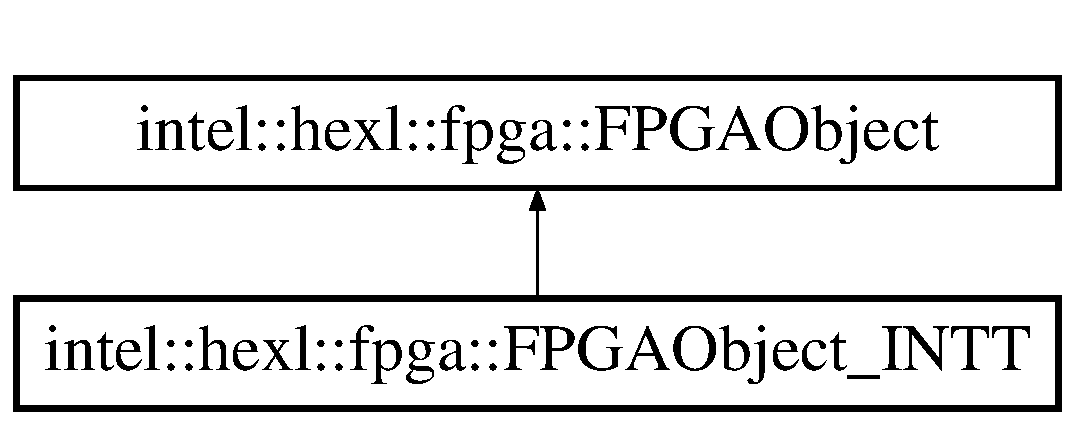
\includegraphics[height=2.000000cm]{structintel_1_1hexl_1_1fpga_1_1FPGAObject__INTT}
\end{center}
\end{figure}
\subsection*{Public Member Functions}
\begin{DoxyCompactItemize}
\item 
\hyperlink{structintel_1_1hexl_1_1fpga_1_1FPGAObject__INTT_a153585cd172743a16e84efd8659aa66c}{F\-P\-G\-A\-Object\-\_\-\-I\-N\-T\-T} (const cl\-\_\-context \&context, uint64\-\_\-t coeff\-\_\-count, uint64\-\_\-t batch\-\_\-size)
\item 
\hyperlink{structintel_1_1hexl_1_1fpga_1_1FPGAObject__INTT_a7cedf64bc8c7af8f1a77dd68e9dd2037}{$\sim$\-F\-P\-G\-A\-Object\-\_\-\-I\-N\-T\-T} ()
\item 
\hyperlink{structintel_1_1hexl_1_1fpga_1_1FPGAObject__INTT_a991d2f78abe5d44b4f98f3b4ac4da29e}{F\-P\-G\-A\-Object\-\_\-\-I\-N\-T\-T} (const \hyperlink{structintel_1_1hexl_1_1fpga_1_1FPGAObject__INTT}{F\-P\-G\-A\-Object\-\_\-\-I\-N\-T\-T} \&)=delete
\item 
\hyperlink{structintel_1_1hexl_1_1fpga_1_1FPGAObject__INTT}{F\-P\-G\-A\-Object\-\_\-\-I\-N\-T\-T} \& \hyperlink{structintel_1_1hexl_1_1fpga_1_1FPGAObject__INTT_af77e8207b17014631d1251ecf6c375f8}{operator=} (const \hyperlink{structintel_1_1hexl_1_1fpga_1_1FPGAObject__INTT}{F\-P\-G\-A\-Object\-\_\-\-I\-N\-T\-T} \&)=delete
\item 
void \hyperlink{structintel_1_1hexl_1_1fpga_1_1FPGAObject__INTT_a3af9d73a583150a06fee9288a7938e31}{fill\-\_\-in\-\_\-data} (const std\-::vector$<$ \hyperlink{structintel_1_1hexl_1_1fpga_1_1Object}{Object} $\ast$ $>$ \&objs) override
\item 
void \hyperlink{structintel_1_1hexl_1_1fpga_1_1FPGAObject__INTT_a18c10384468f7e39f15b2059fe59d5db}{fill\-\_\-out\-\_\-data} (uint64\-\_\-t $\ast$coeff\-\_\-poly) override
\end{DoxyCompactItemize}
\subsection*{Public Attributes}
\begin{DoxyCompactItemize}
\item 
uint64\-\_\-t $\ast$ \hyperlink{structintel_1_1hexl_1_1fpga_1_1FPGAObject__INTT_a5da6fc4cb5bebebb021c6cc2b94bbd7a}{coeff\-\_\-poly\-\_\-in\-\_\-svm\-\_\-}
\item 
uint64\-\_\-t $\ast$ \hyperlink{structintel_1_1hexl_1_1fpga_1_1FPGAObject__INTT_ab85ed19766b48f1cd854a07786b59f8f}{inv\-\_\-root\-\_\-of\-\_\-unity\-\_\-powers\-\_\-in\-\_\-svm\-\_\-}
\item 
uint64\-\_\-t $\ast$ \hyperlink{structintel_1_1hexl_1_1fpga_1_1FPGAObject__INTT_a9a18cf43978c3d56bad1e3494e25859a}{precon\-\_\-inv\-\_\-root\-\_\-of\-\_\-unity\-\_\-powers\-\_\-in\-\_\-svm\-\_\-}
\item 
uint64\-\_\-t $\ast$ \hyperlink{structintel_1_1hexl_1_1fpga_1_1FPGAObject__INTT_a7a893fbe1ec584f7fb59e49dfce3d45e}{coeff\-\_\-modulus\-\_\-in\-\_\-svm\-\_\-}
\item 
uint64\-\_\-t $\ast$ \hyperlink{structintel_1_1hexl_1_1fpga_1_1FPGAObject__INTT_af7b22e09b44bad334bbf2597619b74fd}{inv\-\_\-n\-\_\-in\-\_\-svm\-\_\-}
\item 
uint64\-\_\-t $\ast$ \hyperlink{structintel_1_1hexl_1_1fpga_1_1FPGAObject__INTT_a4d7e4702797bb9e28dd27436e8d981e6}{inv\-\_\-n\-\_\-w\-\_\-in\-\_\-svm\-\_\-}
\item 
uint64\-\_\-t \hyperlink{structintel_1_1hexl_1_1fpga_1_1FPGAObject__INTT_a79d41547e934454b4c4719d2a0d1fd4f}{n\-\_\-}
\end{DoxyCompactItemize}
\subsection*{Additional Inherited Members}


\subsection{Detailed Description}
Struct \hyperlink{structintel_1_1hexl_1_1fpga_1_1FPGAObject__INTT}{F\-P\-G\-A\-Object\-\_\-\-I\-N\-T\-T} stores the I\-N\-T\-T blob of objects to be transfered to the F\-P\-G\-A. 

fill\-\_\-in\-\_\-data 
\begin{DoxyParams}[1]{Parameters}
\mbox{\tt in}  & {\em vector} & of objects  fill\-\_\-out\-\_\-data \\
\hline
\mbox{\tt out}  & {\em vector} & of polynomial coefficients\\
\hline
\end{DoxyParams}
coeff\-\_\-poly\-\_\-in\-\_\-svm vector of polynomial coefficients inv\-\_\-root\-\_\-of\-\_\-unity\-\_\-powers\-\_\-in\-\_\-svm twiddle factors precon\-\_\-inv\-\_\-root\-\_\-of\-\_\-unity\-\_\-powers\-\_\-in\-\_\-svm inverse twiddle factors coeff\-\_\-modulus\-\_\-in\-\_\-svm\-\_\- polynomial coefficients modulus inv\-\_\-n\-\_\-in\-\_\-svm\-\_\- normalization factor 1/n for the polynomial coefficients inv\-\_\-n\-\_\-w\-\_\-in\-\_\-svm\-\_\- normalization factor 1/n for the constant coefficient n polynomial size 

\subsection{Constructor \& Destructor Documentation}
\hypertarget{structintel_1_1hexl_1_1fpga_1_1FPGAObject__INTT_a153585cd172743a16e84efd8659aa66c}{\index{intel\-::hexl\-::fpga\-::\-F\-P\-G\-A\-Object\-\_\-\-I\-N\-T\-T@{intel\-::hexl\-::fpga\-::\-F\-P\-G\-A\-Object\-\_\-\-I\-N\-T\-T}!F\-P\-G\-A\-Object\-\_\-\-I\-N\-T\-T@{F\-P\-G\-A\-Object\-\_\-\-I\-N\-T\-T}}
\index{F\-P\-G\-A\-Object\-\_\-\-I\-N\-T\-T@{F\-P\-G\-A\-Object\-\_\-\-I\-N\-T\-T}!intel::hexl::fpga::FPGAObject_INTT@{intel\-::hexl\-::fpga\-::\-F\-P\-G\-A\-Object\-\_\-\-I\-N\-T\-T}}
\subsubsection[{F\-P\-G\-A\-Object\-\_\-\-I\-N\-T\-T}]{\setlength{\rightskip}{0pt plus 5cm}intel\-::hexl\-::fpga\-::\-F\-P\-G\-A\-Object\-\_\-\-I\-N\-T\-T\-::\-F\-P\-G\-A\-Object\-\_\-\-I\-N\-T\-T (
\begin{DoxyParamCaption}
\item[{const cl\-\_\-context \&}]{context, }
\item[{uint64\-\_\-t}]{coeff\-\_\-count, }
\item[{uint64\-\_\-t}]{batch\-\_\-size}
\end{DoxyParamCaption}
)\hspace{0.3cm}{\ttfamily [explicit]}}}\label{structintel_1_1hexl_1_1fpga_1_1FPGAObject__INTT_a153585cd172743a16e84efd8659aa66c}
\hypertarget{structintel_1_1hexl_1_1fpga_1_1FPGAObject__INTT_a7cedf64bc8c7af8f1a77dd68e9dd2037}{\index{intel\-::hexl\-::fpga\-::\-F\-P\-G\-A\-Object\-\_\-\-I\-N\-T\-T@{intel\-::hexl\-::fpga\-::\-F\-P\-G\-A\-Object\-\_\-\-I\-N\-T\-T}!$\sim$\-F\-P\-G\-A\-Object\-\_\-\-I\-N\-T\-T@{$\sim$\-F\-P\-G\-A\-Object\-\_\-\-I\-N\-T\-T}}
\index{$\sim$\-F\-P\-G\-A\-Object\-\_\-\-I\-N\-T\-T@{$\sim$\-F\-P\-G\-A\-Object\-\_\-\-I\-N\-T\-T}!intel::hexl::fpga::FPGAObject_INTT@{intel\-::hexl\-::fpga\-::\-F\-P\-G\-A\-Object\-\_\-\-I\-N\-T\-T}}
\subsubsection[{$\sim$\-F\-P\-G\-A\-Object\-\_\-\-I\-N\-T\-T}]{\setlength{\rightskip}{0pt plus 5cm}intel\-::hexl\-::fpga\-::\-F\-P\-G\-A\-Object\-\_\-\-I\-N\-T\-T\-::$\sim$\-F\-P\-G\-A\-Object\-\_\-\-I\-N\-T\-T (
\begin{DoxyParamCaption}
{}
\end{DoxyParamCaption}
)}}\label{structintel_1_1hexl_1_1fpga_1_1FPGAObject__INTT_a7cedf64bc8c7af8f1a77dd68e9dd2037}
\hypertarget{structintel_1_1hexl_1_1fpga_1_1FPGAObject__INTT_a991d2f78abe5d44b4f98f3b4ac4da29e}{\index{intel\-::hexl\-::fpga\-::\-F\-P\-G\-A\-Object\-\_\-\-I\-N\-T\-T@{intel\-::hexl\-::fpga\-::\-F\-P\-G\-A\-Object\-\_\-\-I\-N\-T\-T}!F\-P\-G\-A\-Object\-\_\-\-I\-N\-T\-T@{F\-P\-G\-A\-Object\-\_\-\-I\-N\-T\-T}}
\index{F\-P\-G\-A\-Object\-\_\-\-I\-N\-T\-T@{F\-P\-G\-A\-Object\-\_\-\-I\-N\-T\-T}!intel::hexl::fpga::FPGAObject_INTT@{intel\-::hexl\-::fpga\-::\-F\-P\-G\-A\-Object\-\_\-\-I\-N\-T\-T}}
\subsubsection[{F\-P\-G\-A\-Object\-\_\-\-I\-N\-T\-T}]{\setlength{\rightskip}{0pt plus 5cm}intel\-::hexl\-::fpga\-::\-F\-P\-G\-A\-Object\-\_\-\-I\-N\-T\-T\-::\-F\-P\-G\-A\-Object\-\_\-\-I\-N\-T\-T (
\begin{DoxyParamCaption}
\item[{const {\bf F\-P\-G\-A\-Object\-\_\-\-I\-N\-T\-T} \&}]{}
\end{DoxyParamCaption}
)\hspace{0.3cm}{\ttfamily [delete]}}}\label{structintel_1_1hexl_1_1fpga_1_1FPGAObject__INTT_a991d2f78abe5d44b4f98f3b4ac4da29e}


\subsection{Member Function Documentation}
\hypertarget{structintel_1_1hexl_1_1fpga_1_1FPGAObject__INTT_a3af9d73a583150a06fee9288a7938e31}{\index{intel\-::hexl\-::fpga\-::\-F\-P\-G\-A\-Object\-\_\-\-I\-N\-T\-T@{intel\-::hexl\-::fpga\-::\-F\-P\-G\-A\-Object\-\_\-\-I\-N\-T\-T}!fill\-\_\-in\-\_\-data@{fill\-\_\-in\-\_\-data}}
\index{fill\-\_\-in\-\_\-data@{fill\-\_\-in\-\_\-data}!intel::hexl::fpga::FPGAObject_INTT@{intel\-::hexl\-::fpga\-::\-F\-P\-G\-A\-Object\-\_\-\-I\-N\-T\-T}}
\subsubsection[{fill\-\_\-in\-\_\-data}]{\setlength{\rightskip}{0pt plus 5cm}void intel\-::hexl\-::fpga\-::\-F\-P\-G\-A\-Object\-\_\-\-I\-N\-T\-T\-::fill\-\_\-in\-\_\-data (
\begin{DoxyParamCaption}
\item[{const std\-::vector$<$ {\bf Object} $\ast$ $>$ \&}]{objs}
\end{DoxyParamCaption}
)\hspace{0.3cm}{\ttfamily [override]}, {\ttfamily [virtual]}}}\label{structintel_1_1hexl_1_1fpga_1_1FPGAObject__INTT_a3af9d73a583150a06fee9288a7938e31}


Implements \hyperlink{structintel_1_1hexl_1_1fpga_1_1FPGAObject_abd665113bfb3b0e7a33e09078f01ae43}{intel\-::hexl\-::fpga\-::\-F\-P\-G\-A\-Object}.

\hypertarget{structintel_1_1hexl_1_1fpga_1_1FPGAObject__INTT_a18c10384468f7e39f15b2059fe59d5db}{\index{intel\-::hexl\-::fpga\-::\-F\-P\-G\-A\-Object\-\_\-\-I\-N\-T\-T@{intel\-::hexl\-::fpga\-::\-F\-P\-G\-A\-Object\-\_\-\-I\-N\-T\-T}!fill\-\_\-out\-\_\-data@{fill\-\_\-out\-\_\-data}}
\index{fill\-\_\-out\-\_\-data@{fill\-\_\-out\-\_\-data}!intel::hexl::fpga::FPGAObject_INTT@{intel\-::hexl\-::fpga\-::\-F\-P\-G\-A\-Object\-\_\-\-I\-N\-T\-T}}
\subsubsection[{fill\-\_\-out\-\_\-data}]{\setlength{\rightskip}{0pt plus 5cm}void intel\-::hexl\-::fpga\-::\-F\-P\-G\-A\-Object\-\_\-\-I\-N\-T\-T\-::fill\-\_\-out\-\_\-data (
\begin{DoxyParamCaption}
\item[{uint64\-\_\-t $\ast$}]{coeff\-\_\-poly}
\end{DoxyParamCaption}
)\hspace{0.3cm}{\ttfamily [override]}, {\ttfamily [virtual]}}}\label{structintel_1_1hexl_1_1fpga_1_1FPGAObject__INTT_a18c10384468f7e39f15b2059fe59d5db}


Implements \hyperlink{structintel_1_1hexl_1_1fpga_1_1FPGAObject_a954c4c75077a7c406f6c81517ea7bb04}{intel\-::hexl\-::fpga\-::\-F\-P\-G\-A\-Object}.

\hypertarget{structintel_1_1hexl_1_1fpga_1_1FPGAObject__INTT_af77e8207b17014631d1251ecf6c375f8}{\index{intel\-::hexl\-::fpga\-::\-F\-P\-G\-A\-Object\-\_\-\-I\-N\-T\-T@{intel\-::hexl\-::fpga\-::\-F\-P\-G\-A\-Object\-\_\-\-I\-N\-T\-T}!operator=@{operator=}}
\index{operator=@{operator=}!intel::hexl::fpga::FPGAObject_INTT@{intel\-::hexl\-::fpga\-::\-F\-P\-G\-A\-Object\-\_\-\-I\-N\-T\-T}}
\subsubsection[{operator=}]{\setlength{\rightskip}{0pt plus 5cm}{\bf F\-P\-G\-A\-Object\-\_\-\-I\-N\-T\-T}\& intel\-::hexl\-::fpga\-::\-F\-P\-G\-A\-Object\-\_\-\-I\-N\-T\-T\-::operator= (
\begin{DoxyParamCaption}
\item[{const {\bf F\-P\-G\-A\-Object\-\_\-\-I\-N\-T\-T} \&}]{}
\end{DoxyParamCaption}
)\hspace{0.3cm}{\ttfamily [delete]}}}\label{structintel_1_1hexl_1_1fpga_1_1FPGAObject__INTT_af77e8207b17014631d1251ecf6c375f8}


\subsection{Member Data Documentation}
\hypertarget{structintel_1_1hexl_1_1fpga_1_1FPGAObject__INTT_a7a893fbe1ec584f7fb59e49dfce3d45e}{\index{intel\-::hexl\-::fpga\-::\-F\-P\-G\-A\-Object\-\_\-\-I\-N\-T\-T@{intel\-::hexl\-::fpga\-::\-F\-P\-G\-A\-Object\-\_\-\-I\-N\-T\-T}!coeff\-\_\-modulus\-\_\-in\-\_\-svm\-\_\-@{coeff\-\_\-modulus\-\_\-in\-\_\-svm\-\_\-}}
\index{coeff\-\_\-modulus\-\_\-in\-\_\-svm\-\_\-@{coeff\-\_\-modulus\-\_\-in\-\_\-svm\-\_\-}!intel::hexl::fpga::FPGAObject_INTT@{intel\-::hexl\-::fpga\-::\-F\-P\-G\-A\-Object\-\_\-\-I\-N\-T\-T}}
\subsubsection[{coeff\-\_\-modulus\-\_\-in\-\_\-svm\-\_\-}]{\setlength{\rightskip}{0pt plus 5cm}uint64\-\_\-t$\ast$ intel\-::hexl\-::fpga\-::\-F\-P\-G\-A\-Object\-\_\-\-I\-N\-T\-T\-::coeff\-\_\-modulus\-\_\-in\-\_\-svm\-\_\-}}\label{structintel_1_1hexl_1_1fpga_1_1FPGAObject__INTT_a7a893fbe1ec584f7fb59e49dfce3d45e}
\hypertarget{structintel_1_1hexl_1_1fpga_1_1FPGAObject__INTT_a5da6fc4cb5bebebb021c6cc2b94bbd7a}{\index{intel\-::hexl\-::fpga\-::\-F\-P\-G\-A\-Object\-\_\-\-I\-N\-T\-T@{intel\-::hexl\-::fpga\-::\-F\-P\-G\-A\-Object\-\_\-\-I\-N\-T\-T}!coeff\-\_\-poly\-\_\-in\-\_\-svm\-\_\-@{coeff\-\_\-poly\-\_\-in\-\_\-svm\-\_\-}}
\index{coeff\-\_\-poly\-\_\-in\-\_\-svm\-\_\-@{coeff\-\_\-poly\-\_\-in\-\_\-svm\-\_\-}!intel::hexl::fpga::FPGAObject_INTT@{intel\-::hexl\-::fpga\-::\-F\-P\-G\-A\-Object\-\_\-\-I\-N\-T\-T}}
\subsubsection[{coeff\-\_\-poly\-\_\-in\-\_\-svm\-\_\-}]{\setlength{\rightskip}{0pt plus 5cm}uint64\-\_\-t$\ast$ intel\-::hexl\-::fpga\-::\-F\-P\-G\-A\-Object\-\_\-\-I\-N\-T\-T\-::coeff\-\_\-poly\-\_\-in\-\_\-svm\-\_\-}}\label{structintel_1_1hexl_1_1fpga_1_1FPGAObject__INTT_a5da6fc4cb5bebebb021c6cc2b94bbd7a}
\hypertarget{structintel_1_1hexl_1_1fpga_1_1FPGAObject__INTT_af7b22e09b44bad334bbf2597619b74fd}{\index{intel\-::hexl\-::fpga\-::\-F\-P\-G\-A\-Object\-\_\-\-I\-N\-T\-T@{intel\-::hexl\-::fpga\-::\-F\-P\-G\-A\-Object\-\_\-\-I\-N\-T\-T}!inv\-\_\-n\-\_\-in\-\_\-svm\-\_\-@{inv\-\_\-n\-\_\-in\-\_\-svm\-\_\-}}
\index{inv\-\_\-n\-\_\-in\-\_\-svm\-\_\-@{inv\-\_\-n\-\_\-in\-\_\-svm\-\_\-}!intel::hexl::fpga::FPGAObject_INTT@{intel\-::hexl\-::fpga\-::\-F\-P\-G\-A\-Object\-\_\-\-I\-N\-T\-T}}
\subsubsection[{inv\-\_\-n\-\_\-in\-\_\-svm\-\_\-}]{\setlength{\rightskip}{0pt plus 5cm}uint64\-\_\-t$\ast$ intel\-::hexl\-::fpga\-::\-F\-P\-G\-A\-Object\-\_\-\-I\-N\-T\-T\-::inv\-\_\-n\-\_\-in\-\_\-svm\-\_\-}}\label{structintel_1_1hexl_1_1fpga_1_1FPGAObject__INTT_af7b22e09b44bad334bbf2597619b74fd}
\hypertarget{structintel_1_1hexl_1_1fpga_1_1FPGAObject__INTT_a4d7e4702797bb9e28dd27436e8d981e6}{\index{intel\-::hexl\-::fpga\-::\-F\-P\-G\-A\-Object\-\_\-\-I\-N\-T\-T@{intel\-::hexl\-::fpga\-::\-F\-P\-G\-A\-Object\-\_\-\-I\-N\-T\-T}!inv\-\_\-n\-\_\-w\-\_\-in\-\_\-svm\-\_\-@{inv\-\_\-n\-\_\-w\-\_\-in\-\_\-svm\-\_\-}}
\index{inv\-\_\-n\-\_\-w\-\_\-in\-\_\-svm\-\_\-@{inv\-\_\-n\-\_\-w\-\_\-in\-\_\-svm\-\_\-}!intel::hexl::fpga::FPGAObject_INTT@{intel\-::hexl\-::fpga\-::\-F\-P\-G\-A\-Object\-\_\-\-I\-N\-T\-T}}
\subsubsection[{inv\-\_\-n\-\_\-w\-\_\-in\-\_\-svm\-\_\-}]{\setlength{\rightskip}{0pt plus 5cm}uint64\-\_\-t$\ast$ intel\-::hexl\-::fpga\-::\-F\-P\-G\-A\-Object\-\_\-\-I\-N\-T\-T\-::inv\-\_\-n\-\_\-w\-\_\-in\-\_\-svm\-\_\-}}\label{structintel_1_1hexl_1_1fpga_1_1FPGAObject__INTT_a4d7e4702797bb9e28dd27436e8d981e6}
\hypertarget{structintel_1_1hexl_1_1fpga_1_1FPGAObject__INTT_ab85ed19766b48f1cd854a07786b59f8f}{\index{intel\-::hexl\-::fpga\-::\-F\-P\-G\-A\-Object\-\_\-\-I\-N\-T\-T@{intel\-::hexl\-::fpga\-::\-F\-P\-G\-A\-Object\-\_\-\-I\-N\-T\-T}!inv\-\_\-root\-\_\-of\-\_\-unity\-\_\-powers\-\_\-in\-\_\-svm\-\_\-@{inv\-\_\-root\-\_\-of\-\_\-unity\-\_\-powers\-\_\-in\-\_\-svm\-\_\-}}
\index{inv\-\_\-root\-\_\-of\-\_\-unity\-\_\-powers\-\_\-in\-\_\-svm\-\_\-@{inv\-\_\-root\-\_\-of\-\_\-unity\-\_\-powers\-\_\-in\-\_\-svm\-\_\-}!intel::hexl::fpga::FPGAObject_INTT@{intel\-::hexl\-::fpga\-::\-F\-P\-G\-A\-Object\-\_\-\-I\-N\-T\-T}}
\subsubsection[{inv\-\_\-root\-\_\-of\-\_\-unity\-\_\-powers\-\_\-in\-\_\-svm\-\_\-}]{\setlength{\rightskip}{0pt plus 5cm}uint64\-\_\-t$\ast$ intel\-::hexl\-::fpga\-::\-F\-P\-G\-A\-Object\-\_\-\-I\-N\-T\-T\-::inv\-\_\-root\-\_\-of\-\_\-unity\-\_\-powers\-\_\-in\-\_\-svm\-\_\-}}\label{structintel_1_1hexl_1_1fpga_1_1FPGAObject__INTT_ab85ed19766b48f1cd854a07786b59f8f}
\hypertarget{structintel_1_1hexl_1_1fpga_1_1FPGAObject__INTT_a79d41547e934454b4c4719d2a0d1fd4f}{\index{intel\-::hexl\-::fpga\-::\-F\-P\-G\-A\-Object\-\_\-\-I\-N\-T\-T@{intel\-::hexl\-::fpga\-::\-F\-P\-G\-A\-Object\-\_\-\-I\-N\-T\-T}!n\-\_\-@{n\-\_\-}}
\index{n\-\_\-@{n\-\_\-}!intel::hexl::fpga::FPGAObject_INTT@{intel\-::hexl\-::fpga\-::\-F\-P\-G\-A\-Object\-\_\-\-I\-N\-T\-T}}
\subsubsection[{n\-\_\-}]{\setlength{\rightskip}{0pt plus 5cm}uint64\-\_\-t intel\-::hexl\-::fpga\-::\-F\-P\-G\-A\-Object\-\_\-\-I\-N\-T\-T\-::n\-\_\-}}\label{structintel_1_1hexl_1_1fpga_1_1FPGAObject__INTT_a79d41547e934454b4c4719d2a0d1fd4f}
\hypertarget{structintel_1_1hexl_1_1fpga_1_1FPGAObject__INTT_a9a18cf43978c3d56bad1e3494e25859a}{\index{intel\-::hexl\-::fpga\-::\-F\-P\-G\-A\-Object\-\_\-\-I\-N\-T\-T@{intel\-::hexl\-::fpga\-::\-F\-P\-G\-A\-Object\-\_\-\-I\-N\-T\-T}!precon\-\_\-inv\-\_\-root\-\_\-of\-\_\-unity\-\_\-powers\-\_\-in\-\_\-svm\-\_\-@{precon\-\_\-inv\-\_\-root\-\_\-of\-\_\-unity\-\_\-powers\-\_\-in\-\_\-svm\-\_\-}}
\index{precon\-\_\-inv\-\_\-root\-\_\-of\-\_\-unity\-\_\-powers\-\_\-in\-\_\-svm\-\_\-@{precon\-\_\-inv\-\_\-root\-\_\-of\-\_\-unity\-\_\-powers\-\_\-in\-\_\-svm\-\_\-}!intel::hexl::fpga::FPGAObject_INTT@{intel\-::hexl\-::fpga\-::\-F\-P\-G\-A\-Object\-\_\-\-I\-N\-T\-T}}
\subsubsection[{precon\-\_\-inv\-\_\-root\-\_\-of\-\_\-unity\-\_\-powers\-\_\-in\-\_\-svm\-\_\-}]{\setlength{\rightskip}{0pt plus 5cm}uint64\-\_\-t$\ast$ intel\-::hexl\-::fpga\-::\-F\-P\-G\-A\-Object\-\_\-\-I\-N\-T\-T\-::precon\-\_\-inv\-\_\-root\-\_\-of\-\_\-unity\-\_\-powers\-\_\-in\-\_\-svm\-\_\-}}\label{structintel_1_1hexl_1_1fpga_1_1FPGAObject__INTT_a9a18cf43978c3d56bad1e3494e25859a}


The documentation for this struct was generated from the following file\-:\begin{DoxyCompactItemize}
\item 
\hyperlink{fpga_8h}{fpga.\-h}\end{DoxyCompactItemize}

\hypertarget{structintel_1_1hexl_1_1fpga_1_1FPGAObject__NTT}{\section{intel\-:\-:hexl\-:\-:fpga\-:\-:F\-P\-G\-A\-Object\-\_\-\-N\-T\-T Struct Reference}
\label{structintel_1_1hexl_1_1fpga_1_1FPGAObject__NTT}\index{intel\-::hexl\-::fpga\-::\-F\-P\-G\-A\-Object\-\_\-\-N\-T\-T@{intel\-::hexl\-::fpga\-::\-F\-P\-G\-A\-Object\-\_\-\-N\-T\-T}}
}


Struct \hyperlink{structintel_1_1hexl_1_1fpga_1_1FPGAObject__NTT}{F\-P\-G\-A\-Object\-\_\-\-N\-T\-T} stores the N\-T\-T blob of objects to be transfered to the F\-P\-G\-A.  




{\ttfamily \#include $<$fpga.\-h$>$}

Inheritance diagram for intel\-:\-:hexl\-:\-:fpga\-:\-:F\-P\-G\-A\-Object\-\_\-\-N\-T\-T\-:\begin{figure}[H]
\begin{center}
\leavevmode
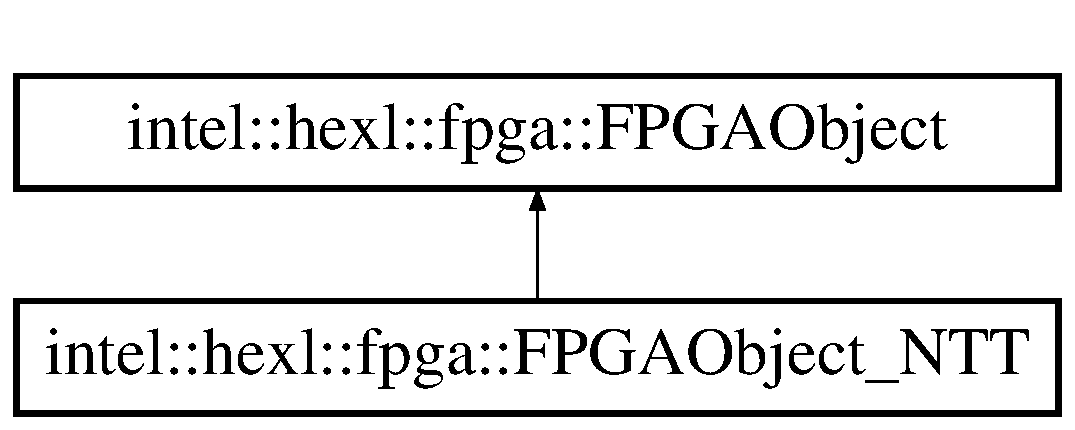
\includegraphics[height=2.000000cm]{structintel_1_1hexl_1_1fpga_1_1FPGAObject__NTT}
\end{center}
\end{figure}
\subsection*{Public Member Functions}
\begin{DoxyCompactItemize}
\item 
\hyperlink{structintel_1_1hexl_1_1fpga_1_1FPGAObject__NTT_a0ea057e0cc2e3a1b13917ac8f1bd1af3}{F\-P\-G\-A\-Object\-\_\-\-N\-T\-T} (const cl\-\_\-context \&context, uint64\-\_\-t coeff\-\_\-count, uint64\-\_\-t batch\-\_\-size)
\item 
\hyperlink{structintel_1_1hexl_1_1fpga_1_1FPGAObject__NTT_abae77f82236fa240111b32bd1b665a21}{$\sim$\-F\-P\-G\-A\-Object\-\_\-\-N\-T\-T} ()
\item 
void \hyperlink{structintel_1_1hexl_1_1fpga_1_1FPGAObject__NTT_a3aa5e6c85ae154bcf98ba99205feda16}{fill\-\_\-in\-\_\-data} (const std\-::vector$<$ \hyperlink{structintel_1_1hexl_1_1fpga_1_1Object}{Object} $\ast$ $>$ \&objs) override
\item 
void \hyperlink{structintel_1_1hexl_1_1fpga_1_1FPGAObject__NTT_a4f31676fdaf820560f625d2f468da397}{fill\-\_\-out\-\_\-data} (uint64\-\_\-t $\ast$coeff\-\_\-poly) override
\end{DoxyCompactItemize}
\subsection*{Public Attributes}
\begin{DoxyCompactItemize}
\item 
uint64\-\_\-t $\ast$ \hyperlink{structintel_1_1hexl_1_1fpga_1_1FPGAObject__NTT_a899dea2730faece216ae48d60bb14b07}{coeff\-\_\-poly\-\_\-in\-\_\-svm\-\_\-}
\item 
uint64\-\_\-t $\ast$ \hyperlink{structintel_1_1hexl_1_1fpga_1_1FPGAObject__NTT_a1263c41528af5e32878a535d5422b33d}{root\-\_\-of\-\_\-unity\-\_\-powers\-\_\-in\-\_\-svm\-\_\-}
\item 
uint64\-\_\-t $\ast$ \hyperlink{structintel_1_1hexl_1_1fpga_1_1FPGAObject__NTT_a7ac4c0e1180cf9b29998f1e2ae1c074c}{precon\-\_\-root\-\_\-of\-\_\-unity\-\_\-powers\-\_\-in\-\_\-svm\-\_\-}
\item 
uint64\-\_\-t $\ast$ \hyperlink{structintel_1_1hexl_1_1fpga_1_1FPGAObject__NTT_aef6ec35bf5733224ffd5d1be64de4ab1}{coeff\-\_\-modulus\-\_\-in\-\_\-svm\-\_\-}
\item 
uint64\-\_\-t \hyperlink{structintel_1_1hexl_1_1fpga_1_1FPGAObject__NTT_aa7b2933a6ad042a0ec97aa5b7eff3c5e}{n\-\_\-}
\end{DoxyCompactItemize}
\subsection*{Additional Inherited Members}


\subsection{Detailed Description}
Struct \hyperlink{structintel_1_1hexl_1_1fpga_1_1FPGAObject__NTT}{F\-P\-G\-A\-Object\-\_\-\-N\-T\-T} stores the N\-T\-T blob of objects to be transfered to the F\-P\-G\-A. 

fill\-\_\-in\-\_\-data 
\begin{DoxyParams}[1]{Parameters}
\mbox{\tt in}  & {\em vector} & of objects  fill\-\_\-out\-\_\-data \\
\hline
\mbox{\tt out}  & {\em vector} & of polynomial coefficients\\
\hline
\end{DoxyParams}
coeff\-\_\-poly\-\_\-in\-\_\-svm vector of polynomial coefficients root\-\_\-of\-\_\-unity\-\_\-powers\-\_\-in\-\_\-svm twiddle factors precon\-\_\-root\-\_\-of\-\_\-unity\-\_\-powers\-\_\-in\-\_\-svm inverse twiddle factors coeff\-\_\-modulus\-\_\-in\-\_\-svm\-\_\- polynomial coefficients modulus n polynomial size 

\subsection{Constructor \& Destructor Documentation}
\hypertarget{structintel_1_1hexl_1_1fpga_1_1FPGAObject__NTT_a0ea057e0cc2e3a1b13917ac8f1bd1af3}{\index{intel\-::hexl\-::fpga\-::\-F\-P\-G\-A\-Object\-\_\-\-N\-T\-T@{intel\-::hexl\-::fpga\-::\-F\-P\-G\-A\-Object\-\_\-\-N\-T\-T}!F\-P\-G\-A\-Object\-\_\-\-N\-T\-T@{F\-P\-G\-A\-Object\-\_\-\-N\-T\-T}}
\index{F\-P\-G\-A\-Object\-\_\-\-N\-T\-T@{F\-P\-G\-A\-Object\-\_\-\-N\-T\-T}!intel::hexl::fpga::FPGAObject_NTT@{intel\-::hexl\-::fpga\-::\-F\-P\-G\-A\-Object\-\_\-\-N\-T\-T}}
\subsubsection[{F\-P\-G\-A\-Object\-\_\-\-N\-T\-T}]{\setlength{\rightskip}{0pt plus 5cm}intel\-::hexl\-::fpga\-::\-F\-P\-G\-A\-Object\-\_\-\-N\-T\-T\-::\-F\-P\-G\-A\-Object\-\_\-\-N\-T\-T (
\begin{DoxyParamCaption}
\item[{const cl\-\_\-context \&}]{context, }
\item[{uint64\-\_\-t}]{coeff\-\_\-count, }
\item[{uint64\-\_\-t}]{batch\-\_\-size}
\end{DoxyParamCaption}
)\hspace{0.3cm}{\ttfamily [explicit]}}}\label{structintel_1_1hexl_1_1fpga_1_1FPGAObject__NTT_a0ea057e0cc2e3a1b13917ac8f1bd1af3}
\hypertarget{structintel_1_1hexl_1_1fpga_1_1FPGAObject__NTT_abae77f82236fa240111b32bd1b665a21}{\index{intel\-::hexl\-::fpga\-::\-F\-P\-G\-A\-Object\-\_\-\-N\-T\-T@{intel\-::hexl\-::fpga\-::\-F\-P\-G\-A\-Object\-\_\-\-N\-T\-T}!$\sim$\-F\-P\-G\-A\-Object\-\_\-\-N\-T\-T@{$\sim$\-F\-P\-G\-A\-Object\-\_\-\-N\-T\-T}}
\index{$\sim$\-F\-P\-G\-A\-Object\-\_\-\-N\-T\-T@{$\sim$\-F\-P\-G\-A\-Object\-\_\-\-N\-T\-T}!intel::hexl::fpga::FPGAObject_NTT@{intel\-::hexl\-::fpga\-::\-F\-P\-G\-A\-Object\-\_\-\-N\-T\-T}}
\subsubsection[{$\sim$\-F\-P\-G\-A\-Object\-\_\-\-N\-T\-T}]{\setlength{\rightskip}{0pt plus 5cm}intel\-::hexl\-::fpga\-::\-F\-P\-G\-A\-Object\-\_\-\-N\-T\-T\-::$\sim$\-F\-P\-G\-A\-Object\-\_\-\-N\-T\-T (
\begin{DoxyParamCaption}
{}
\end{DoxyParamCaption}
)}}\label{structintel_1_1hexl_1_1fpga_1_1FPGAObject__NTT_abae77f82236fa240111b32bd1b665a21}


\subsection{Member Function Documentation}
\hypertarget{structintel_1_1hexl_1_1fpga_1_1FPGAObject__NTT_a3aa5e6c85ae154bcf98ba99205feda16}{\index{intel\-::hexl\-::fpga\-::\-F\-P\-G\-A\-Object\-\_\-\-N\-T\-T@{intel\-::hexl\-::fpga\-::\-F\-P\-G\-A\-Object\-\_\-\-N\-T\-T}!fill\-\_\-in\-\_\-data@{fill\-\_\-in\-\_\-data}}
\index{fill\-\_\-in\-\_\-data@{fill\-\_\-in\-\_\-data}!intel::hexl::fpga::FPGAObject_NTT@{intel\-::hexl\-::fpga\-::\-F\-P\-G\-A\-Object\-\_\-\-N\-T\-T}}
\subsubsection[{fill\-\_\-in\-\_\-data}]{\setlength{\rightskip}{0pt plus 5cm}void intel\-::hexl\-::fpga\-::\-F\-P\-G\-A\-Object\-\_\-\-N\-T\-T\-::fill\-\_\-in\-\_\-data (
\begin{DoxyParamCaption}
\item[{const std\-::vector$<$ {\bf Object} $\ast$ $>$ \&}]{objs}
\end{DoxyParamCaption}
)\hspace{0.3cm}{\ttfamily [override]}, {\ttfamily [virtual]}}}\label{structintel_1_1hexl_1_1fpga_1_1FPGAObject__NTT_a3aa5e6c85ae154bcf98ba99205feda16}


Implements \hyperlink{structintel_1_1hexl_1_1fpga_1_1FPGAObject_abd665113bfb3b0e7a33e09078f01ae43}{intel\-::hexl\-::fpga\-::\-F\-P\-G\-A\-Object}.

\hypertarget{structintel_1_1hexl_1_1fpga_1_1FPGAObject__NTT_a4f31676fdaf820560f625d2f468da397}{\index{intel\-::hexl\-::fpga\-::\-F\-P\-G\-A\-Object\-\_\-\-N\-T\-T@{intel\-::hexl\-::fpga\-::\-F\-P\-G\-A\-Object\-\_\-\-N\-T\-T}!fill\-\_\-out\-\_\-data@{fill\-\_\-out\-\_\-data}}
\index{fill\-\_\-out\-\_\-data@{fill\-\_\-out\-\_\-data}!intel::hexl::fpga::FPGAObject_NTT@{intel\-::hexl\-::fpga\-::\-F\-P\-G\-A\-Object\-\_\-\-N\-T\-T}}
\subsubsection[{fill\-\_\-out\-\_\-data}]{\setlength{\rightskip}{0pt plus 5cm}void intel\-::hexl\-::fpga\-::\-F\-P\-G\-A\-Object\-\_\-\-N\-T\-T\-::fill\-\_\-out\-\_\-data (
\begin{DoxyParamCaption}
\item[{uint64\-\_\-t $\ast$}]{coeff\-\_\-poly}
\end{DoxyParamCaption}
)\hspace{0.3cm}{\ttfamily [override]}, {\ttfamily [virtual]}}}\label{structintel_1_1hexl_1_1fpga_1_1FPGAObject__NTT_a4f31676fdaf820560f625d2f468da397}


Implements \hyperlink{structintel_1_1hexl_1_1fpga_1_1FPGAObject_a954c4c75077a7c406f6c81517ea7bb04}{intel\-::hexl\-::fpga\-::\-F\-P\-G\-A\-Object}.



\subsection{Member Data Documentation}
\hypertarget{structintel_1_1hexl_1_1fpga_1_1FPGAObject__NTT_aef6ec35bf5733224ffd5d1be64de4ab1}{\index{intel\-::hexl\-::fpga\-::\-F\-P\-G\-A\-Object\-\_\-\-N\-T\-T@{intel\-::hexl\-::fpga\-::\-F\-P\-G\-A\-Object\-\_\-\-N\-T\-T}!coeff\-\_\-modulus\-\_\-in\-\_\-svm\-\_\-@{coeff\-\_\-modulus\-\_\-in\-\_\-svm\-\_\-}}
\index{coeff\-\_\-modulus\-\_\-in\-\_\-svm\-\_\-@{coeff\-\_\-modulus\-\_\-in\-\_\-svm\-\_\-}!intel::hexl::fpga::FPGAObject_NTT@{intel\-::hexl\-::fpga\-::\-F\-P\-G\-A\-Object\-\_\-\-N\-T\-T}}
\subsubsection[{coeff\-\_\-modulus\-\_\-in\-\_\-svm\-\_\-}]{\setlength{\rightskip}{0pt plus 5cm}uint64\-\_\-t$\ast$ intel\-::hexl\-::fpga\-::\-F\-P\-G\-A\-Object\-\_\-\-N\-T\-T\-::coeff\-\_\-modulus\-\_\-in\-\_\-svm\-\_\-}}\label{structintel_1_1hexl_1_1fpga_1_1FPGAObject__NTT_aef6ec35bf5733224ffd5d1be64de4ab1}
\hypertarget{structintel_1_1hexl_1_1fpga_1_1FPGAObject__NTT_a899dea2730faece216ae48d60bb14b07}{\index{intel\-::hexl\-::fpga\-::\-F\-P\-G\-A\-Object\-\_\-\-N\-T\-T@{intel\-::hexl\-::fpga\-::\-F\-P\-G\-A\-Object\-\_\-\-N\-T\-T}!coeff\-\_\-poly\-\_\-in\-\_\-svm\-\_\-@{coeff\-\_\-poly\-\_\-in\-\_\-svm\-\_\-}}
\index{coeff\-\_\-poly\-\_\-in\-\_\-svm\-\_\-@{coeff\-\_\-poly\-\_\-in\-\_\-svm\-\_\-}!intel::hexl::fpga::FPGAObject_NTT@{intel\-::hexl\-::fpga\-::\-F\-P\-G\-A\-Object\-\_\-\-N\-T\-T}}
\subsubsection[{coeff\-\_\-poly\-\_\-in\-\_\-svm\-\_\-}]{\setlength{\rightskip}{0pt plus 5cm}uint64\-\_\-t$\ast$ intel\-::hexl\-::fpga\-::\-F\-P\-G\-A\-Object\-\_\-\-N\-T\-T\-::coeff\-\_\-poly\-\_\-in\-\_\-svm\-\_\-}}\label{structintel_1_1hexl_1_1fpga_1_1FPGAObject__NTT_a899dea2730faece216ae48d60bb14b07}
\hypertarget{structintel_1_1hexl_1_1fpga_1_1FPGAObject__NTT_aa7b2933a6ad042a0ec97aa5b7eff3c5e}{\index{intel\-::hexl\-::fpga\-::\-F\-P\-G\-A\-Object\-\_\-\-N\-T\-T@{intel\-::hexl\-::fpga\-::\-F\-P\-G\-A\-Object\-\_\-\-N\-T\-T}!n\-\_\-@{n\-\_\-}}
\index{n\-\_\-@{n\-\_\-}!intel::hexl::fpga::FPGAObject_NTT@{intel\-::hexl\-::fpga\-::\-F\-P\-G\-A\-Object\-\_\-\-N\-T\-T}}
\subsubsection[{n\-\_\-}]{\setlength{\rightskip}{0pt plus 5cm}uint64\-\_\-t intel\-::hexl\-::fpga\-::\-F\-P\-G\-A\-Object\-\_\-\-N\-T\-T\-::n\-\_\-}}\label{structintel_1_1hexl_1_1fpga_1_1FPGAObject__NTT_aa7b2933a6ad042a0ec97aa5b7eff3c5e}
\hypertarget{structintel_1_1hexl_1_1fpga_1_1FPGAObject__NTT_a7ac4c0e1180cf9b29998f1e2ae1c074c}{\index{intel\-::hexl\-::fpga\-::\-F\-P\-G\-A\-Object\-\_\-\-N\-T\-T@{intel\-::hexl\-::fpga\-::\-F\-P\-G\-A\-Object\-\_\-\-N\-T\-T}!precon\-\_\-root\-\_\-of\-\_\-unity\-\_\-powers\-\_\-in\-\_\-svm\-\_\-@{precon\-\_\-root\-\_\-of\-\_\-unity\-\_\-powers\-\_\-in\-\_\-svm\-\_\-}}
\index{precon\-\_\-root\-\_\-of\-\_\-unity\-\_\-powers\-\_\-in\-\_\-svm\-\_\-@{precon\-\_\-root\-\_\-of\-\_\-unity\-\_\-powers\-\_\-in\-\_\-svm\-\_\-}!intel::hexl::fpga::FPGAObject_NTT@{intel\-::hexl\-::fpga\-::\-F\-P\-G\-A\-Object\-\_\-\-N\-T\-T}}
\subsubsection[{precon\-\_\-root\-\_\-of\-\_\-unity\-\_\-powers\-\_\-in\-\_\-svm\-\_\-}]{\setlength{\rightskip}{0pt plus 5cm}uint64\-\_\-t$\ast$ intel\-::hexl\-::fpga\-::\-F\-P\-G\-A\-Object\-\_\-\-N\-T\-T\-::precon\-\_\-root\-\_\-of\-\_\-unity\-\_\-powers\-\_\-in\-\_\-svm\-\_\-}}\label{structintel_1_1hexl_1_1fpga_1_1FPGAObject__NTT_a7ac4c0e1180cf9b29998f1e2ae1c074c}
\hypertarget{structintel_1_1hexl_1_1fpga_1_1FPGAObject__NTT_a1263c41528af5e32878a535d5422b33d}{\index{intel\-::hexl\-::fpga\-::\-F\-P\-G\-A\-Object\-\_\-\-N\-T\-T@{intel\-::hexl\-::fpga\-::\-F\-P\-G\-A\-Object\-\_\-\-N\-T\-T}!root\-\_\-of\-\_\-unity\-\_\-powers\-\_\-in\-\_\-svm\-\_\-@{root\-\_\-of\-\_\-unity\-\_\-powers\-\_\-in\-\_\-svm\-\_\-}}
\index{root\-\_\-of\-\_\-unity\-\_\-powers\-\_\-in\-\_\-svm\-\_\-@{root\-\_\-of\-\_\-unity\-\_\-powers\-\_\-in\-\_\-svm\-\_\-}!intel::hexl::fpga::FPGAObject_NTT@{intel\-::hexl\-::fpga\-::\-F\-P\-G\-A\-Object\-\_\-\-N\-T\-T}}
\subsubsection[{root\-\_\-of\-\_\-unity\-\_\-powers\-\_\-in\-\_\-svm\-\_\-}]{\setlength{\rightskip}{0pt plus 5cm}uint64\-\_\-t$\ast$ intel\-::hexl\-::fpga\-::\-F\-P\-G\-A\-Object\-\_\-\-N\-T\-T\-::root\-\_\-of\-\_\-unity\-\_\-powers\-\_\-in\-\_\-svm\-\_\-}}\label{structintel_1_1hexl_1_1fpga_1_1FPGAObject__NTT_a1263c41528af5e32878a535d5422b33d}


The documentation for this struct was generated from the following file\-:\begin{DoxyCompactItemize}
\item 
\hyperlink{fpga_8h}{fpga.\-h}\end{DoxyCompactItemize}

\hypertarget{classfwd__ntt__test}{\section{fwd\-\_\-ntt\-\_\-test Class Reference}
\label{classfwd__ntt__test}\index{fwd\-\_\-ntt\-\_\-test@{fwd\-\_\-ntt\-\_\-test}}
}
Inheritance diagram for fwd\-\_\-ntt\-\_\-test\-:\begin{figure}[H]
\begin{center}
\leavevmode
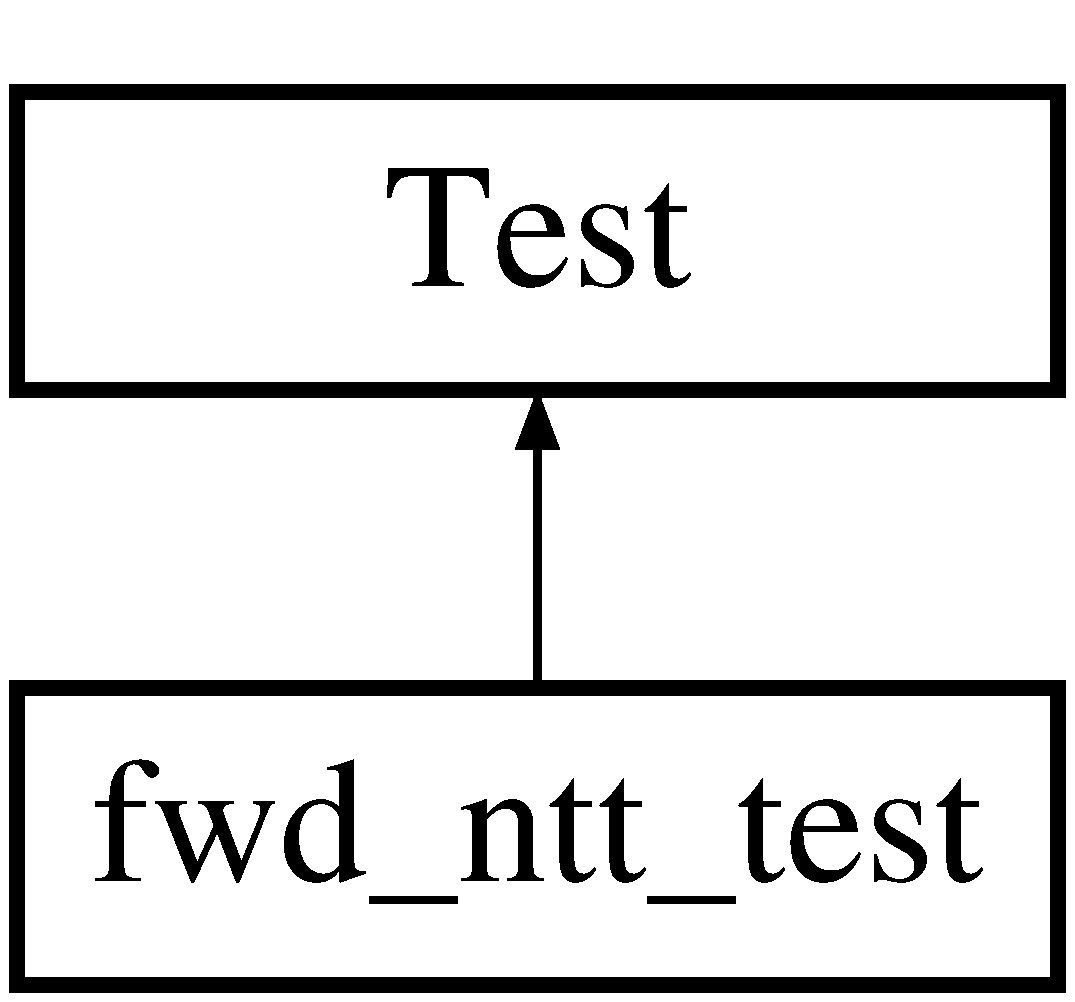
\includegraphics[height=2.000000cm]{classfwd__ntt__test}
\end{center}
\end{figure}
\subsection*{Public Member Functions}
\begin{DoxyCompactItemize}
\item 
void \hyperlink{classfwd__ntt__test_afd48a701b23f9e9efd2e64aaded2cd32}{run\-\_\-fwd\-\_\-ntt\-\_\-test} (\hyperlink{namespacehetest_1_1utils_a17ac57eb86d3ead191cb51163ef63eb0}{Stimulus\-Type} stimulus\-Type, uint64\-\_\-t iterations, uint64\-\_\-t bits\-For\-Prime)
\item 
void \hyperlink{classfwd__ntt__test_a9edfd258d90a49382602613427a49111}{Test\-Body} () override
\end{DoxyCompactItemize}


\subsection{Member Function Documentation}
\hypertarget{classfwd__ntt__test_afd48a701b23f9e9efd2e64aaded2cd32}{\index{fwd\-\_\-ntt\-\_\-test@{fwd\-\_\-ntt\-\_\-test}!run\-\_\-fwd\-\_\-ntt\-\_\-test@{run\-\_\-fwd\-\_\-ntt\-\_\-test}}
\index{run\-\_\-fwd\-\_\-ntt\-\_\-test@{run\-\_\-fwd\-\_\-ntt\-\_\-test}!fwd_ntt_test@{fwd\-\_\-ntt\-\_\-test}}
\subsubsection[{run\-\_\-fwd\-\_\-ntt\-\_\-test}]{\setlength{\rightskip}{0pt plus 5cm}void fwd\-\_\-ntt\-\_\-test\-::run\-\_\-fwd\-\_\-ntt\-\_\-test (
\begin{DoxyParamCaption}
\item[{{\bf Stimulus\-Type}}]{stimulus\-Type, }
\item[{uint64\-\_\-t}]{iterations, }
\item[{uint64\-\_\-t}]{bits\-For\-Prime}
\end{DoxyParamCaption}
)}}\label{classfwd__ntt__test_afd48a701b23f9e9efd2e64aaded2cd32}
\hypertarget{classfwd__ntt__test_a9edfd258d90a49382602613427a49111}{\index{fwd\-\_\-ntt\-\_\-test@{fwd\-\_\-ntt\-\_\-test}!Test\-Body@{Test\-Body}}
\index{Test\-Body@{Test\-Body}!fwd_ntt_test@{fwd\-\_\-ntt\-\_\-test}}
\subsubsection[{Test\-Body}]{\setlength{\rightskip}{0pt plus 5cm}void fwd\-\_\-ntt\-\_\-test\-::\-Test\-Body (
\begin{DoxyParamCaption}
{}
\end{DoxyParamCaption}
)\hspace{0.3cm}{\ttfamily [inline]}, {\ttfamily [override]}}}\label{classfwd__ntt__test_a9edfd258d90a49382602613427a49111}


The documentation for this class was generated from the following file\-:\begin{DoxyCompactItemize}
\item 
\hyperlink{test__fwd__ntt_8cpp}{test\-\_\-fwd\-\_\-ntt.\-cpp}\end{DoxyCompactItemize}

\hypertarget{classhexl__fpga}{\section{hexl\-\_\-fpga Class Reference}
\label{classhexl__fpga}\index{hexl\-\_\-fpga@{hexl\-\_\-fpga}}
}
Inheritance diagram for hexl\-\_\-fpga\-:\begin{figure}[H]
\begin{center}
\leavevmode
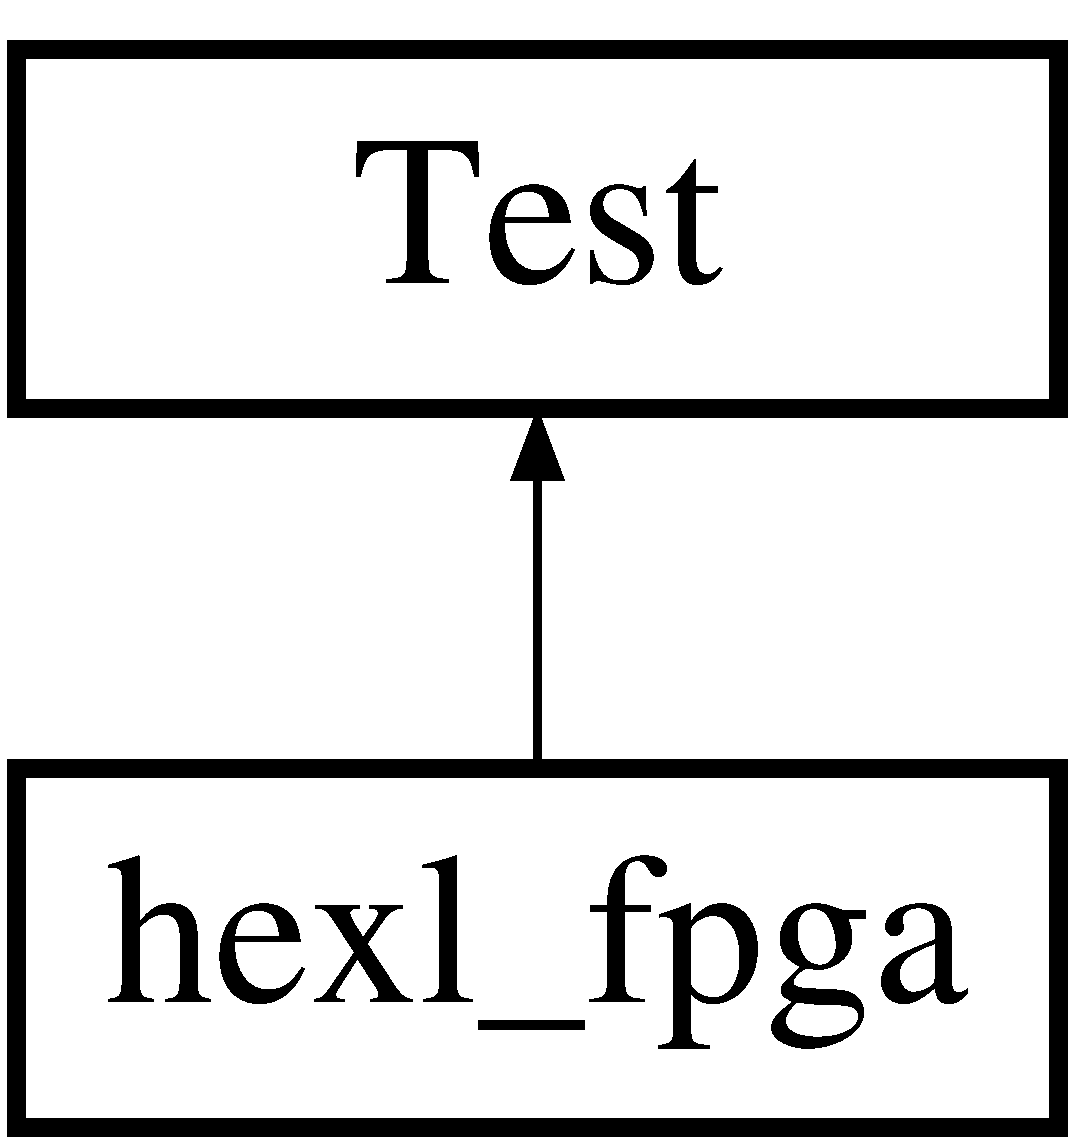
\includegraphics[height=2.000000cm]{classhexl__fpga}
\end{center}
\end{figure}
\subsection*{Public Member Functions}
\begin{DoxyCompactItemize}
\item 
void \hyperlink{classhexl__fpga_a9ddbb55f9f613de66114dc4e559b69c3}{ntt\-\_\-test} ()
\item 
void \hyperlink{classhexl__fpga_a91390d80f8d6bba6917bf67df13972f0}{Test\-Body} () override
\end{DoxyCompactItemize}


\subsection{Member Function Documentation}
\hypertarget{classhexl__fpga_a9ddbb55f9f613de66114dc4e559b69c3}{\index{hexl\-\_\-fpga@{hexl\-\_\-fpga}!ntt\-\_\-test@{ntt\-\_\-test}}
\index{ntt\-\_\-test@{ntt\-\_\-test}!hexl_fpga@{hexl\-\_\-fpga}}
\subsubsection[{ntt\-\_\-test}]{\setlength{\rightskip}{0pt plus 5cm}void hexl\-\_\-fpga\-::ntt\-\_\-test (
\begin{DoxyParamCaption}
{}
\end{DoxyParamCaption}
)}}\label{classhexl__fpga_a9ddbb55f9f613de66114dc4e559b69c3}
\hypertarget{classhexl__fpga_a91390d80f8d6bba6917bf67df13972f0}{\index{hexl\-\_\-fpga@{hexl\-\_\-fpga}!Test\-Body@{Test\-Body}}
\index{Test\-Body@{Test\-Body}!hexl_fpga@{hexl\-\_\-fpga}}
\subsubsection[{Test\-Body}]{\setlength{\rightskip}{0pt plus 5cm}void hexl\-\_\-fpga\-::\-Test\-Body (
\begin{DoxyParamCaption}
{}
\end{DoxyParamCaption}
)\hspace{0.3cm}{\ttfamily [inline]}, {\ttfamily [override]}}}\label{classhexl__fpga_a91390d80f8d6bba6917bf67df13972f0}


The documentation for this class was generated from the following file\-:\begin{DoxyCompactItemize}
\item 
\hyperlink{test__hexl__fpga_8cpp}{test\-\_\-hexl\-\_\-fpga.\-cpp}\end{DoxyCompactItemize}

\hypertarget{classinv__ntt}{\section{inv\-\_\-ntt Class Reference}
\label{classinv__ntt}\index{inv\-\_\-ntt@{inv\-\_\-ntt}}
}
Inheritance diagram for inv\-\_\-ntt\-:\begin{figure}[H]
\begin{center}
\leavevmode
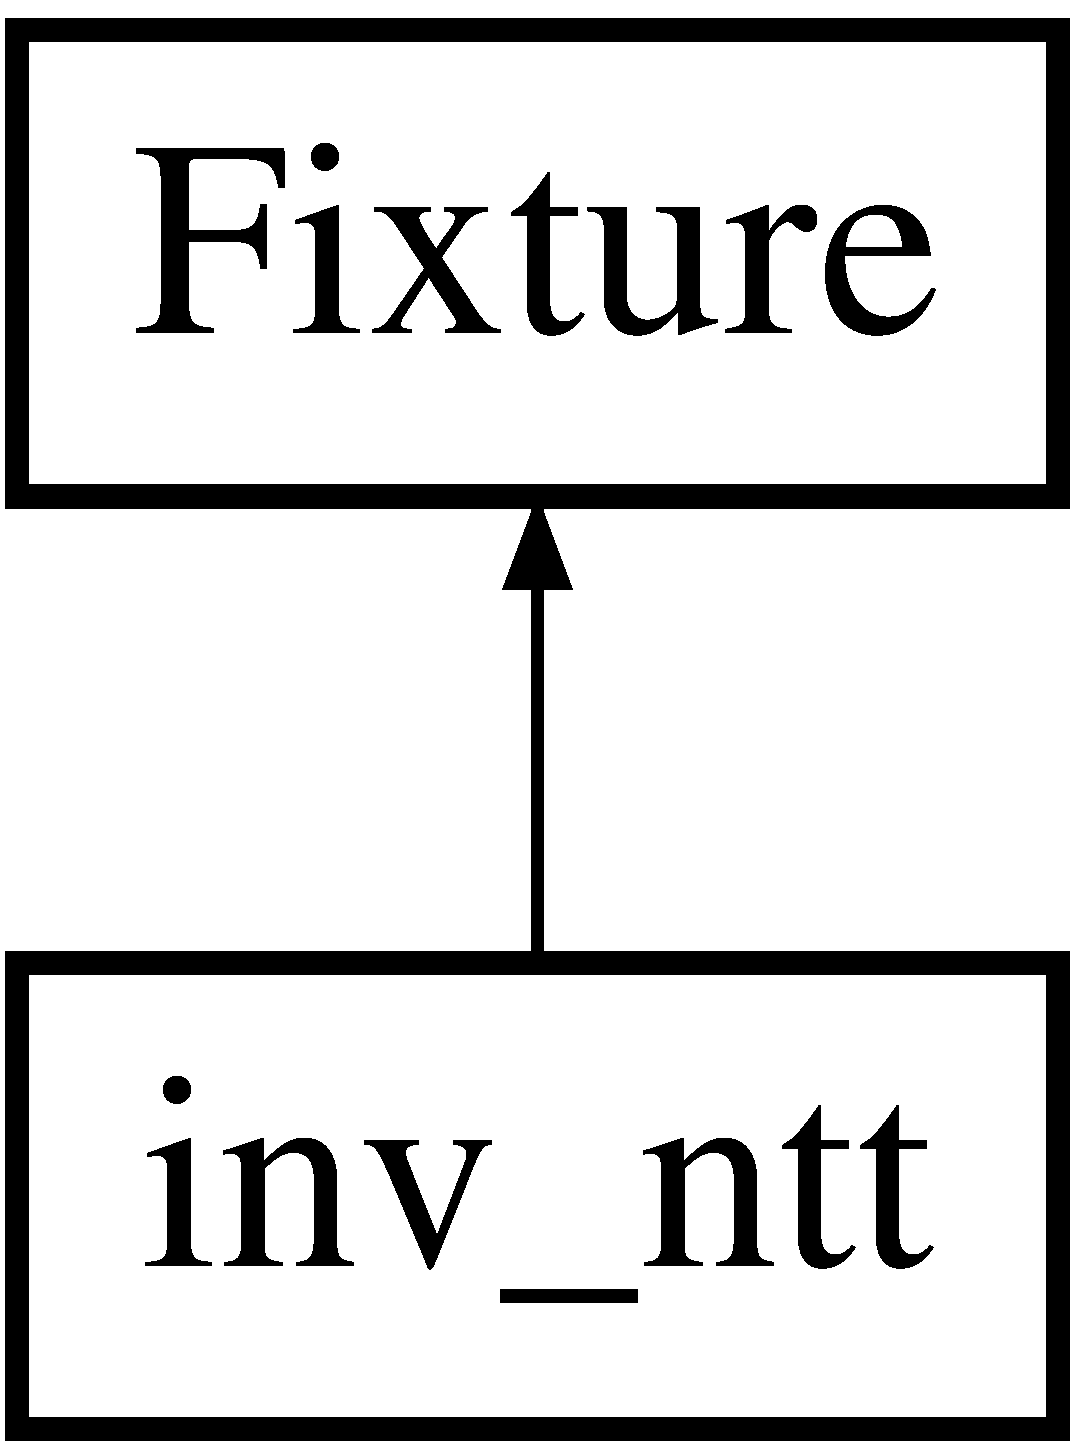
\includegraphics[height=2.000000cm]{classinv__ntt}
\end{center}
\end{figure}
\subsection*{Public Member Functions}
\begin{DoxyCompactItemize}
\item 
void \hyperlink{classinv__ntt_ab6f7a674950aa44f5965286334df341a}{load\-\_\-ntt\-\_\-data} (size\-\_\-t work\-\_\-size)
\item 
void \hyperlink{classinv__ntt_a22e77cf348d2fbf6dad93b8a19b09326}{fpga\-\_\-inv\-\_\-ntt\-\_\-test} (size\-\_\-t work\-\_\-size)
\end{DoxyCompactItemize}


\subsection{Member Function Documentation}
\hypertarget{classinv__ntt_a22e77cf348d2fbf6dad93b8a19b09326}{\index{inv\-\_\-ntt@{inv\-\_\-ntt}!fpga\-\_\-inv\-\_\-ntt\-\_\-test@{fpga\-\_\-inv\-\_\-ntt\-\_\-test}}
\index{fpga\-\_\-inv\-\_\-ntt\-\_\-test@{fpga\-\_\-inv\-\_\-ntt\-\_\-test}!inv_ntt@{inv\-\_\-ntt}}
\subsubsection[{fpga\-\_\-inv\-\_\-ntt\-\_\-test}]{\setlength{\rightskip}{0pt plus 5cm}void inv\-\_\-ntt\-::fpga\-\_\-inv\-\_\-ntt\-\_\-test (
\begin{DoxyParamCaption}
\item[{size\-\_\-t}]{work\-\_\-size}
\end{DoxyParamCaption}
)}}\label{classinv__ntt_a22e77cf348d2fbf6dad93b8a19b09326}
\hypertarget{classinv__ntt_ab6f7a674950aa44f5965286334df341a}{\index{inv\-\_\-ntt@{inv\-\_\-ntt}!load\-\_\-ntt\-\_\-data@{load\-\_\-ntt\-\_\-data}}
\index{load\-\_\-ntt\-\_\-data@{load\-\_\-ntt\-\_\-data}!inv_ntt@{inv\-\_\-ntt}}
\subsubsection[{load\-\_\-ntt\-\_\-data}]{\setlength{\rightskip}{0pt plus 5cm}void inv\-\_\-ntt\-::load\-\_\-ntt\-\_\-data (
\begin{DoxyParamCaption}
\item[{size\-\_\-t}]{work\-\_\-size}
\end{DoxyParamCaption}
)}}\label{classinv__ntt_ab6f7a674950aa44f5965286334df341a}


The documentation for this class was generated from the following file\-:\begin{DoxyCompactItemize}
\item 
\hyperlink{bench__inv__ntt_8cpp}{bench\-\_\-inv\-\_\-ntt.\-cpp}\end{DoxyCompactItemize}

\hypertarget{classinv__ntt__test}{\section{inv\-\_\-ntt\-\_\-test Class Reference}
\label{classinv__ntt__test}\index{inv\-\_\-ntt\-\_\-test@{inv\-\_\-ntt\-\_\-test}}
}
Inheritance diagram for inv\-\_\-ntt\-\_\-test\-:\begin{figure}[H]
\begin{center}
\leavevmode
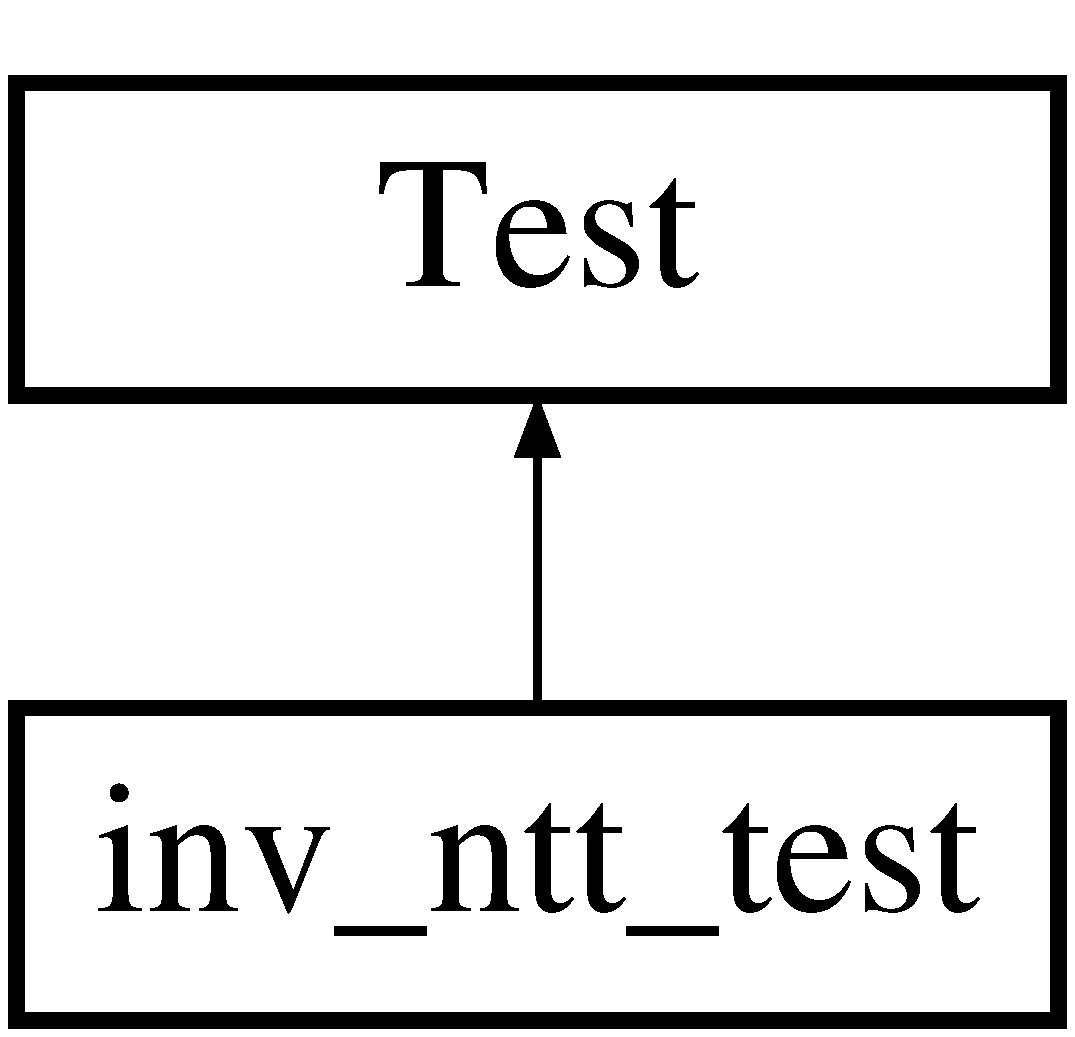
\includegraphics[height=2.000000cm]{classinv__ntt__test}
\end{center}
\end{figure}
\subsection*{Public Member Functions}
\begin{DoxyCompactItemize}
\item 
void \hyperlink{classinv__ntt__test_a8592b35ff857a63e890076cad1b2fdf8}{run\-\_\-inv\-\_\-ntt\-\_\-test} (\hyperlink{namespacehetest_1_1utils_a17ac57eb86d3ead191cb51163ef63eb0}{Stimulus\-Type} stimulus\-Type, uint64\-\_\-t iterations, uint64\-\_\-t bits\-For\-Prime)
\item 
void \hyperlink{classinv__ntt__test_a316de69045abc6a1223fb6360f036eac}{Test\-Body} () override
\end{DoxyCompactItemize}


\subsection{Member Function Documentation}
\hypertarget{classinv__ntt__test_a8592b35ff857a63e890076cad1b2fdf8}{\index{inv\-\_\-ntt\-\_\-test@{inv\-\_\-ntt\-\_\-test}!run\-\_\-inv\-\_\-ntt\-\_\-test@{run\-\_\-inv\-\_\-ntt\-\_\-test}}
\index{run\-\_\-inv\-\_\-ntt\-\_\-test@{run\-\_\-inv\-\_\-ntt\-\_\-test}!inv_ntt_test@{inv\-\_\-ntt\-\_\-test}}
\subsubsection[{run\-\_\-inv\-\_\-ntt\-\_\-test}]{\setlength{\rightskip}{0pt plus 5cm}void inv\-\_\-ntt\-\_\-test\-::run\-\_\-inv\-\_\-ntt\-\_\-test (
\begin{DoxyParamCaption}
\item[{{\bf Stimulus\-Type}}]{stimulus\-Type, }
\item[{uint64\-\_\-t}]{iterations, }
\item[{uint64\-\_\-t}]{bits\-For\-Prime}
\end{DoxyParamCaption}
)}}\label{classinv__ntt__test_a8592b35ff857a63e890076cad1b2fdf8}
\hypertarget{classinv__ntt__test_a316de69045abc6a1223fb6360f036eac}{\index{inv\-\_\-ntt\-\_\-test@{inv\-\_\-ntt\-\_\-test}!Test\-Body@{Test\-Body}}
\index{Test\-Body@{Test\-Body}!inv_ntt_test@{inv\-\_\-ntt\-\_\-test}}
\subsubsection[{Test\-Body}]{\setlength{\rightskip}{0pt plus 5cm}void inv\-\_\-ntt\-\_\-test\-::\-Test\-Body (
\begin{DoxyParamCaption}
{}
\end{DoxyParamCaption}
)\hspace{0.3cm}{\ttfamily [inline]}, {\ttfamily [override]}}}\label{classinv__ntt__test_a316de69045abc6a1223fb6360f036eac}


The documentation for this class was generated from the following file\-:\begin{DoxyCompactItemize}
\item 
\hyperlink{test__inv__ntt_8cpp}{test\-\_\-inv\-\_\-ntt.\-cpp}\end{DoxyCompactItemize}

\hypertarget{structhetest_1_1utils_1_1details_1_1MallocStrategy}{\section{hetest\-:\-:utils\-:\-:details\-:\-:Malloc\-Strategy Struct Reference}
\label{structhetest_1_1utils_1_1details_1_1MallocStrategy}\index{hetest\-::utils\-::details\-::\-Malloc\-Strategy@{hetest\-::utils\-::details\-::\-Malloc\-Strategy}}
}


{\ttfamily \#include $<$utils-\/test.\-hpp$>$}

Inheritance diagram for hetest\-:\-:utils\-:\-:details\-:\-:Malloc\-Strategy\-:\begin{figure}[H]
\begin{center}
\leavevmode
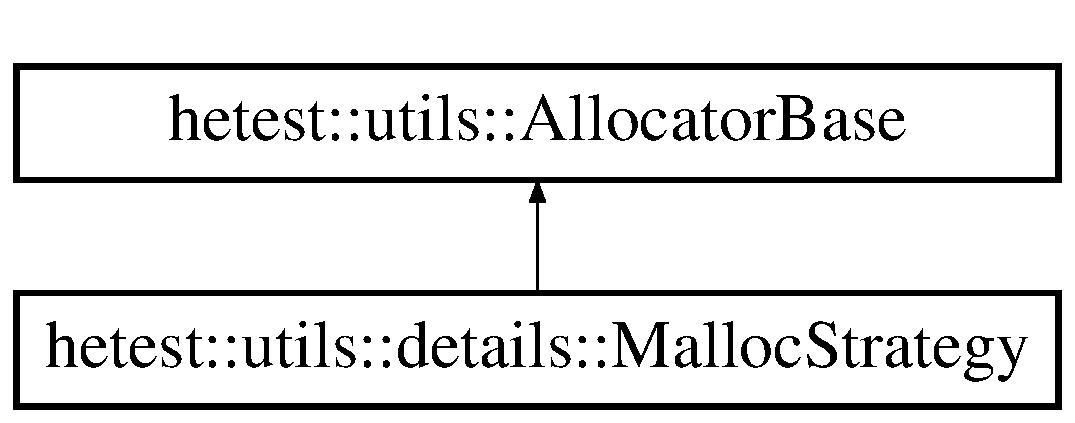
\includegraphics[height=2.000000cm]{structhetest_1_1utils_1_1details_1_1MallocStrategy}
\end{center}
\end{figure}
\subsection*{Public Member Functions}
\begin{DoxyCompactItemize}
\item 
void $\ast$ \hyperlink{structhetest_1_1utils_1_1details_1_1MallocStrategy_a6e72b748596f8ba704363b1aa4d501d9}{allocate} (size\-\_\-t bytes\-\_\-count) final
\item 
void \hyperlink{structhetest_1_1utils_1_1details_1_1MallocStrategy_a86b2b253ec7d4da560da97f6d30e7325}{deallocate} (void $\ast$p, size\-\_\-t n) final
\end{DoxyCompactItemize}


\subsection{Member Function Documentation}
\hypertarget{structhetest_1_1utils_1_1details_1_1MallocStrategy_a6e72b748596f8ba704363b1aa4d501d9}{\index{hetest\-::utils\-::details\-::\-Malloc\-Strategy@{hetest\-::utils\-::details\-::\-Malloc\-Strategy}!allocate@{allocate}}
\index{allocate@{allocate}!hetest::utils::details::MallocStrategy@{hetest\-::utils\-::details\-::\-Malloc\-Strategy}}
\subsubsection[{allocate}]{\setlength{\rightskip}{0pt plus 5cm}void$\ast$ hetest\-::utils\-::details\-::\-Malloc\-Strategy\-::allocate (
\begin{DoxyParamCaption}
\item[{size\-\_\-t}]{bytes\-\_\-count}
\end{DoxyParamCaption}
)\hspace{0.3cm}{\ttfamily [inline]}, {\ttfamily [final]}, {\ttfamily [virtual]}}}\label{structhetest_1_1utils_1_1details_1_1MallocStrategy_a6e72b748596f8ba704363b1aa4d501d9}


Implements \hyperlink{structhetest_1_1utils_1_1AllocatorBase_aa179ce655f57197104fce71166c17374}{hetest\-::utils\-::\-Allocator\-Base}.

\hypertarget{structhetest_1_1utils_1_1details_1_1MallocStrategy_a86b2b253ec7d4da560da97f6d30e7325}{\index{hetest\-::utils\-::details\-::\-Malloc\-Strategy@{hetest\-::utils\-::details\-::\-Malloc\-Strategy}!deallocate@{deallocate}}
\index{deallocate@{deallocate}!hetest::utils::details::MallocStrategy@{hetest\-::utils\-::details\-::\-Malloc\-Strategy}}
\subsubsection[{deallocate}]{\setlength{\rightskip}{0pt plus 5cm}void hetest\-::utils\-::details\-::\-Malloc\-Strategy\-::deallocate (
\begin{DoxyParamCaption}
\item[{void $\ast$}]{p, }
\item[{size\-\_\-t}]{n}
\end{DoxyParamCaption}
)\hspace{0.3cm}{\ttfamily [inline]}, {\ttfamily [final]}, {\ttfamily [virtual]}}}\label{structhetest_1_1utils_1_1details_1_1MallocStrategy_a86b2b253ec7d4da560da97f6d30e7325}


Implements \hyperlink{structhetest_1_1utils_1_1AllocatorBase_ab9e3d2285da2861d0939afe26c6683e4}{hetest\-::utils\-::\-Allocator\-Base}.



The documentation for this struct was generated from the following file\-:\begin{DoxyCompactItemize}
\item 
\hyperlink{utils-test_8hpp}{utils-\/test.\-hpp}\end{DoxyCompactItemize}

\hypertarget{structintel_1_1hexl_1_1fpga_1_1moduli__info__t}{\section{intel\-:\-:hexl\-:\-:fpga\-:\-:moduli\-\_\-info\-\_\-t Struct Reference}
\label{structintel_1_1hexl_1_1fpga_1_1moduli__info__t}\index{intel\-::hexl\-::fpga\-::moduli\-\_\-info\-\_\-t@{intel\-::hexl\-::fpga\-::moduli\-\_\-info\-\_\-t}}
}


Struct \hyperlink{structintel_1_1hexl_1_1fpga_1_1moduli__info__t}{moduli\-\_\-info\-\_\-t}.  




{\ttfamily \#include $<$fpga.\-h$>$}

\subsection*{Public Attributes}
\begin{DoxyCompactItemize}
\item 
uint64\-\_\-t \hyperlink{structintel_1_1hexl_1_1fpga_1_1moduli__info__t_af853b928372ebd6d6f7e5f2d7aa8bba7}{modulus}
\item 
uint64\-\_\-t \hyperlink{structintel_1_1hexl_1_1fpga_1_1moduli__info__t_aeb4594d54e3df5373014386e6addbaa4}{len}
\item 
uint64\-\_\-t \hyperlink{structintel_1_1hexl_1_1fpga_1_1moduli__info__t_ac767dd0d3287329d896e6de911c1f4af}{barr\-\_\-lo}
\end{DoxyCompactItemize}


\subsection{Detailed Description}
Struct \hyperlink{structintel_1_1hexl_1_1fpga_1_1moduli__info__t}{moduli\-\_\-info\-\_\-t}. 


\begin{DoxyParams}[1]{Parameters}
\mbox{\tt in}  & {\em modulus} & stores the polynomial modulus \\
\hline
\mbox{\tt in}  & {\em len} & stores the the modulus size in bits \\
\hline
\mbox{\tt in}  & {\em barr\-\_\-lo} & stores n / modulus where n is the polynomial size \\
\hline
\end{DoxyParams}


\subsection{Member Data Documentation}
\hypertarget{structintel_1_1hexl_1_1fpga_1_1moduli__info__t_ac767dd0d3287329d896e6de911c1f4af}{\index{intel\-::hexl\-::fpga\-::moduli\-\_\-info\-\_\-t@{intel\-::hexl\-::fpga\-::moduli\-\_\-info\-\_\-t}!barr\-\_\-lo@{barr\-\_\-lo}}
\index{barr\-\_\-lo@{barr\-\_\-lo}!intel::hexl::fpga::moduli_info_t@{intel\-::hexl\-::fpga\-::moduli\-\_\-info\-\_\-t}}
\subsubsection[{barr\-\_\-lo}]{\setlength{\rightskip}{0pt plus 5cm}uint64\-\_\-t intel\-::hexl\-::fpga\-::moduli\-\_\-info\-\_\-t\-::barr\-\_\-lo}}\label{structintel_1_1hexl_1_1fpga_1_1moduli__info__t_ac767dd0d3287329d896e6de911c1f4af}
\hypertarget{structintel_1_1hexl_1_1fpga_1_1moduli__info__t_aeb4594d54e3df5373014386e6addbaa4}{\index{intel\-::hexl\-::fpga\-::moduli\-\_\-info\-\_\-t@{intel\-::hexl\-::fpga\-::moduli\-\_\-info\-\_\-t}!len@{len}}
\index{len@{len}!intel::hexl::fpga::moduli_info_t@{intel\-::hexl\-::fpga\-::moduli\-\_\-info\-\_\-t}}
\subsubsection[{len}]{\setlength{\rightskip}{0pt plus 5cm}uint64\-\_\-t intel\-::hexl\-::fpga\-::moduli\-\_\-info\-\_\-t\-::len}}\label{structintel_1_1hexl_1_1fpga_1_1moduli__info__t_aeb4594d54e3df5373014386e6addbaa4}
\hypertarget{structintel_1_1hexl_1_1fpga_1_1moduli__info__t_af853b928372ebd6d6f7e5f2d7aa8bba7}{\index{intel\-::hexl\-::fpga\-::moduli\-\_\-info\-\_\-t@{intel\-::hexl\-::fpga\-::moduli\-\_\-info\-\_\-t}!modulus@{modulus}}
\index{modulus@{modulus}!intel::hexl::fpga::moduli_info_t@{intel\-::hexl\-::fpga\-::moduli\-\_\-info\-\_\-t}}
\subsubsection[{modulus}]{\setlength{\rightskip}{0pt plus 5cm}uint64\-\_\-t intel\-::hexl\-::fpga\-::moduli\-\_\-info\-\_\-t\-::modulus}}\label{structintel_1_1hexl_1_1fpga_1_1moduli__info__t_af853b928372ebd6d6f7e5f2d7aa8bba7}


The documentation for this struct was generated from the following file\-:\begin{DoxyCompactItemize}
\item 
\hyperlink{fpga_8h}{fpga.\-h}\end{DoxyCompactItemize}

\hypertarget{classhetest_1_1utils_1_1MultiplyFactor}{\section{hetest\-:\-:utils\-:\-:Multiply\-Factor Class Reference}
\label{classhetest_1_1utils_1_1MultiplyFactor}\index{hetest\-::utils\-::\-Multiply\-Factor@{hetest\-::utils\-::\-Multiply\-Factor}}
}


{\ttfamily \#include $<$ntt.\-hpp$>$}

\subsection*{Public Member Functions}
\begin{DoxyCompactItemize}
\item 
\hyperlink{classhetest_1_1utils_1_1MultiplyFactor_a86c6f365d618c90d08e52855190be15c}{Multiply\-Factor} ()=default
\item 
\hyperlink{classhetest_1_1utils_1_1MultiplyFactor_aaf6b00666ac003d44f1f71d98fc3c9a1}{Multiply\-Factor} (uint64\-\_\-t operand, uint64\-\_\-t bit\-\_\-shift, uint64\-\_\-t modulus)
\item 
uint64\-\_\-t \hyperlink{classhetest_1_1utils_1_1MultiplyFactor_ae39a0ca3d2b8f97db8e28ed3f1cf9957}{Barrett\-Factor} () const 
\item 
uint64\-\_\-t \hyperlink{classhetest_1_1utils_1_1MultiplyFactor_adb9a6acac4142a551ad70cf9bbb56389}{Operand} () const 
\end{DoxyCompactItemize}


\subsection{Constructor \& Destructor Documentation}
\hypertarget{classhetest_1_1utils_1_1MultiplyFactor_a86c6f365d618c90d08e52855190be15c}{\index{hetest\-::utils\-::\-Multiply\-Factor@{hetest\-::utils\-::\-Multiply\-Factor}!Multiply\-Factor@{Multiply\-Factor}}
\index{Multiply\-Factor@{Multiply\-Factor}!hetest::utils::MultiplyFactor@{hetest\-::utils\-::\-Multiply\-Factor}}
\subsubsection[{Multiply\-Factor}]{\setlength{\rightskip}{0pt plus 5cm}hetest\-::utils\-::\-Multiply\-Factor\-::\-Multiply\-Factor (
\begin{DoxyParamCaption}
{}
\end{DoxyParamCaption}
)\hspace{0.3cm}{\ttfamily [default]}}}\label{classhetest_1_1utils_1_1MultiplyFactor_a86c6f365d618c90d08e52855190be15c}
\hypertarget{classhetest_1_1utils_1_1MultiplyFactor_aaf6b00666ac003d44f1f71d98fc3c9a1}{\index{hetest\-::utils\-::\-Multiply\-Factor@{hetest\-::utils\-::\-Multiply\-Factor}!Multiply\-Factor@{Multiply\-Factor}}
\index{Multiply\-Factor@{Multiply\-Factor}!hetest::utils::MultiplyFactor@{hetest\-::utils\-::\-Multiply\-Factor}}
\subsubsection[{Multiply\-Factor}]{\setlength{\rightskip}{0pt plus 5cm}hetest\-::utils\-::\-Multiply\-Factor\-::\-Multiply\-Factor (
\begin{DoxyParamCaption}
\item[{uint64\-\_\-t}]{operand, }
\item[{uint64\-\_\-t}]{bit\-\_\-shift, }
\item[{uint64\-\_\-t}]{modulus}
\end{DoxyParamCaption}
)\hspace{0.3cm}{\ttfamily [inline]}}}\label{classhetest_1_1utils_1_1MultiplyFactor_aaf6b00666ac003d44f1f71d98fc3c9a1}


\subsection{Member Function Documentation}
\hypertarget{classhetest_1_1utils_1_1MultiplyFactor_ae39a0ca3d2b8f97db8e28ed3f1cf9957}{\index{hetest\-::utils\-::\-Multiply\-Factor@{hetest\-::utils\-::\-Multiply\-Factor}!Barrett\-Factor@{Barrett\-Factor}}
\index{Barrett\-Factor@{Barrett\-Factor}!hetest::utils::MultiplyFactor@{hetest\-::utils\-::\-Multiply\-Factor}}
\subsubsection[{Barrett\-Factor}]{\setlength{\rightskip}{0pt plus 5cm}uint64\-\_\-t hetest\-::utils\-::\-Multiply\-Factor\-::\-Barrett\-Factor (
\begin{DoxyParamCaption}
{}
\end{DoxyParamCaption}
) const\hspace{0.3cm}{\ttfamily [inline]}}}\label{classhetest_1_1utils_1_1MultiplyFactor_ae39a0ca3d2b8f97db8e28ed3f1cf9957}
\hypertarget{classhetest_1_1utils_1_1MultiplyFactor_adb9a6acac4142a551ad70cf9bbb56389}{\index{hetest\-::utils\-::\-Multiply\-Factor@{hetest\-::utils\-::\-Multiply\-Factor}!Operand@{Operand}}
\index{Operand@{Operand}!hetest::utils::MultiplyFactor@{hetest\-::utils\-::\-Multiply\-Factor}}
\subsubsection[{Operand}]{\setlength{\rightskip}{0pt plus 5cm}uint64\-\_\-t hetest\-::utils\-::\-Multiply\-Factor\-::\-Operand (
\begin{DoxyParamCaption}
{}
\end{DoxyParamCaption}
) const\hspace{0.3cm}{\ttfamily [inline]}}}\label{classhetest_1_1utils_1_1MultiplyFactor_adb9a6acac4142a551ad70cf9bbb56389}


The documentation for this class was generated from the following file\-:\begin{DoxyCompactItemize}
\item 
\hyperlink{ntt_8hpp}{ntt.\-hpp}\end{DoxyCompactItemize}

\hypertarget{classhetest_1_1utils_1_1NTT}{\section{hetest\-:\-:utils\-:\-:N\-T\-T Class Reference}
\label{classhetest_1_1utils_1_1NTT}\index{hetest\-::utils\-::\-N\-T\-T@{hetest\-::utils\-::\-N\-T\-T}}
}


Performs negacyclic forward and inverse number-\/theoretic transform (\hyperlink{classhetest_1_1utils_1_1NTT}{N\-T\-T}), commonly used in R\-L\-W\-E cryptography.  




{\ttfamily \#include $<$ntt.\-hpp$>$}

\subsection*{Classes}
\begin{DoxyCompactItemize}
\item 
struct \hyperlink{structhetest_1_1utils_1_1NTT_1_1AllocatorAdapter}{Allocator\-Adapter}
\item 
class \hyperlink{classhetest_1_1utils_1_1NTT_1_1NTTImpl}{N\-T\-T\-Impl}
\end{DoxyCompactItemize}
\subsection*{Public Member Functions}
\begin{DoxyCompactItemize}
\item 
\hyperlink{classhetest_1_1utils_1_1NTT_a3babb9b273fca5c7a7b8c782341e57c0}{N\-T\-T} ()
\begin{DoxyCompactList}\small\item\em Initializes an empty \hyperlink{classhetest_1_1utils_1_1NTT}{N\-T\-T} object. \end{DoxyCompactList}\item 
\hyperlink{classhetest_1_1utils_1_1NTT_af1677329c3f6051d20cf6ce6b28e6c94}{$\sim$\-N\-T\-T} ()
\begin{DoxyCompactList}\small\item\em Destructs the \hyperlink{classhetest_1_1utils_1_1NTT}{N\-T\-T} object. \end{DoxyCompactList}\item 
\hyperlink{classhetest_1_1utils_1_1NTT_a5a974237b1ea73b6e08b33e99356293f}{N\-T\-T} (uint64\-\_\-t degree, uint64\-\_\-t q, std\-::shared\-\_\-ptr$<$ \hyperlink{structhetest_1_1utils_1_1AllocatorBase}{Allocator\-Base} $>$ alloc\-\_\-ptr=\{\})
\begin{DoxyCompactList}\small\item\em Performs pre-\/computation necessary for forward and inverse transforms. \end{DoxyCompactList}\item 
{\footnotesize template$<$class Allocator , class... Allocator\-Args$>$ }\\\hyperlink{classhetest_1_1utils_1_1NTT_a4735b3c9e5f15f9ec0d474a0342b046d}{N\-T\-T} (uint64\-\_\-t degree, uint64\-\_\-t q, Allocator \&\&a, Allocator\-Args \&\&...args)
\item 
\hyperlink{classhetest_1_1utils_1_1NTT_a4f41af61203de2aa28e0d380b5b04ae4}{N\-T\-T} (uint64\-\_\-t degree, uint64\-\_\-t q, uint64\-\_\-t root\-\_\-of\-\_\-unity, std\-::shared\-\_\-ptr$<$ \hyperlink{structhetest_1_1utils_1_1AllocatorBase}{Allocator\-Base} $>$ alloc\-\_\-ptr=\{\})
\begin{DoxyCompactList}\small\item\em Initializes an \hyperlink{classhetest_1_1utils_1_1NTT}{N\-T\-T} object with degree {\ttfamily degree} and modulus {\ttfamily q}. \end{DoxyCompactList}\item 
{\footnotesize template$<$class Allocator , class... Allocator\-Args$>$ }\\\hyperlink{classhetest_1_1utils_1_1NTT_a9877fee08ac585be045a20d8b561d8d1}{N\-T\-T} (uint64\-\_\-t degree, uint64\-\_\-t q, uint64\-\_\-t root\-\_\-of\-\_\-unity, Allocator \&\&a, Allocator\-Args \&\&...args)
\item 
void \hyperlink{classhetest_1_1utils_1_1NTT_af23d2bdd9a1a5ca7fa8d5b7333776ad4}{Compute\-Forward} (uint64\-\_\-t $\ast$result, const uint64\-\_\-t $\ast$operand, uint64\-\_\-t input\-\_\-mod\-\_\-factor, uint64\-\_\-t output\-\_\-mod\-\_\-factor)
\begin{DoxyCompactList}\small\item\em Compute forward \hyperlink{classhetest_1_1utils_1_1NTT}{N\-T\-T}. Results are bit-\/reversed. \end{DoxyCompactList}\item 
void \hyperlink{classhetest_1_1utils_1_1NTT_a0452a339ac9025c750decbb6e011148b}{Compute\-Inverse} (uint64\-\_\-t $\ast$result, const uint64\-\_\-t $\ast$operand, uint64\-\_\-t input\-\_\-mod\-\_\-factor, uint64\-\_\-t output\-\_\-mod\-\_\-factor)
\end{DoxyCompactItemize}
\subsection*{Public Attributes}
\begin{DoxyCompactItemize}
\item 
std\-::shared\-\_\-ptr$<$ \hyperlink{classhetest_1_1utils_1_1NTT_1_1NTTImpl}{N\-T\-T\-Impl} $>$ \hyperlink{classhetest_1_1utils_1_1NTT_ae2d7985d8380a7c30cb0ca745aa900f5}{m\-\_\-impl}
\begin{DoxyCompactList}\small\item\em Class implementing the \hyperlink{classhetest_1_1utils_1_1NTT}{N\-T\-T}. \end{DoxyCompactList}\end{DoxyCompactItemize}


\subsection{Detailed Description}
Performs negacyclic forward and inverse number-\/theoretic transform (\hyperlink{classhetest_1_1utils_1_1NTT}{N\-T\-T}), commonly used in R\-L\-W\-E cryptography. 

The number-\/theoretic transform (\hyperlink{classhetest_1_1utils_1_1NTT}{N\-T\-T}) specializes the discrete Fourier transform (D\-F\-T) to the finite field $ \mathbb{Z}_q[X] / (X^N + 1) $. 

\subsection{Constructor \& Destructor Documentation}
\hypertarget{classhetest_1_1utils_1_1NTT_a3babb9b273fca5c7a7b8c782341e57c0}{\index{hetest\-::utils\-::\-N\-T\-T@{hetest\-::utils\-::\-N\-T\-T}!N\-T\-T@{N\-T\-T}}
\index{N\-T\-T@{N\-T\-T}!hetest::utils::NTT@{hetest\-::utils\-::\-N\-T\-T}}
\subsubsection[{N\-T\-T}]{\setlength{\rightskip}{0pt plus 5cm}hetest\-::utils\-::\-N\-T\-T\-::\-N\-T\-T (
\begin{DoxyParamCaption}
{}
\end{DoxyParamCaption}
)\hspace{0.3cm}{\ttfamily [default]}}}\label{classhetest_1_1utils_1_1NTT_a3babb9b273fca5c7a7b8c782341e57c0}


Initializes an empty \hyperlink{classhetest_1_1utils_1_1NTT}{N\-T\-T} object. 

\hypertarget{classhetest_1_1utils_1_1NTT_af1677329c3f6051d20cf6ce6b28e6c94}{\index{hetest\-::utils\-::\-N\-T\-T@{hetest\-::utils\-::\-N\-T\-T}!$\sim$\-N\-T\-T@{$\sim$\-N\-T\-T}}
\index{$\sim$\-N\-T\-T@{$\sim$\-N\-T\-T}!hetest::utils::NTT@{hetest\-::utils\-::\-N\-T\-T}}
\subsubsection[{$\sim$\-N\-T\-T}]{\setlength{\rightskip}{0pt plus 5cm}hetest\-::utils\-::\-N\-T\-T\-::$\sim$\-N\-T\-T (
\begin{DoxyParamCaption}
{}
\end{DoxyParamCaption}
)\hspace{0.3cm}{\ttfamily [default]}}}\label{classhetest_1_1utils_1_1NTT_af1677329c3f6051d20cf6ce6b28e6c94}


Destructs the \hyperlink{classhetest_1_1utils_1_1NTT}{N\-T\-T} object. 

\hypertarget{classhetest_1_1utils_1_1NTT_a5a974237b1ea73b6e08b33e99356293f}{\index{hetest\-::utils\-::\-N\-T\-T@{hetest\-::utils\-::\-N\-T\-T}!N\-T\-T@{N\-T\-T}}
\index{N\-T\-T@{N\-T\-T}!hetest::utils::NTT@{hetest\-::utils\-::\-N\-T\-T}}
\subsubsection[{N\-T\-T}]{\setlength{\rightskip}{0pt plus 5cm}hetest\-::utils\-::\-N\-T\-T\-::\-N\-T\-T (
\begin{DoxyParamCaption}
\item[{uint64\-\_\-t}]{degree, }
\item[{uint64\-\_\-t}]{q, }
\item[{std\-::shared\-\_\-ptr$<$ {\bf Allocator\-Base} $>$}]{alloc\-\_\-ptr = {\ttfamily \{\}}}
\end{DoxyParamCaption}
)}}\label{classhetest_1_1utils_1_1NTT_a5a974237b1ea73b6e08b33e99356293f}


Performs pre-\/computation necessary for forward and inverse transforms. 

Initializes an \hyperlink{classhetest_1_1utils_1_1NTT}{N\-T\-T} object with degree {\ttfamily degree} and modulus {\ttfamily q}. 
\begin{DoxyParams}[1]{Parameters}
\mbox{\tt in}  & {\em degree} & also known as N. Size of the \hyperlink{classhetest_1_1utils_1_1NTT}{N\-T\-T} transform. Must be a power of 2 \\
\hline
\mbox{\tt in}  & {\em q} & Prime modulus. Must satisfy $ q == 1 \mod 2N $ \\
\hline
\mbox{\tt in}  & {\em alloc\-\_\-ptr} & Custom memory allocator used for intermediate calculations \\
\hline
\end{DoxyParams}
\hypertarget{classhetest_1_1utils_1_1NTT_a4735b3c9e5f15f9ec0d474a0342b046d}{\index{hetest\-::utils\-::\-N\-T\-T@{hetest\-::utils\-::\-N\-T\-T}!N\-T\-T@{N\-T\-T}}
\index{N\-T\-T@{N\-T\-T}!hetest::utils::NTT@{hetest\-::utils\-::\-N\-T\-T}}
\subsubsection[{N\-T\-T}]{\setlength{\rightskip}{0pt plus 5cm}template$<$class Allocator , class... Allocator\-Args$>$ hetest\-::utils\-::\-N\-T\-T\-::\-N\-T\-T (
\begin{DoxyParamCaption}
\item[{uint64\-\_\-t}]{degree, }
\item[{uint64\-\_\-t}]{q, }
\item[{Allocator \&\&}]{a, }
\item[{Allocator\-Args \&\&...}]{args}
\end{DoxyParamCaption}
)\hspace{0.3cm}{\ttfamily [inline]}}}\label{classhetest_1_1utils_1_1NTT_a4735b3c9e5f15f9ec0d474a0342b046d}
\hypertarget{classhetest_1_1utils_1_1NTT_a4f41af61203de2aa28e0d380b5b04ae4}{\index{hetest\-::utils\-::\-N\-T\-T@{hetest\-::utils\-::\-N\-T\-T}!N\-T\-T@{N\-T\-T}}
\index{N\-T\-T@{N\-T\-T}!hetest::utils::NTT@{hetest\-::utils\-::\-N\-T\-T}}
\subsubsection[{N\-T\-T}]{\setlength{\rightskip}{0pt plus 5cm}hetest\-::utils\-::\-N\-T\-T\-::\-N\-T\-T (
\begin{DoxyParamCaption}
\item[{uint64\-\_\-t}]{degree, }
\item[{uint64\-\_\-t}]{q, }
\item[{uint64\-\_\-t}]{root\-\_\-of\-\_\-unity, }
\item[{std\-::shared\-\_\-ptr$<$ {\bf Allocator\-Base} $>$}]{alloc\-\_\-ptr = {\ttfamily \{\}}}
\end{DoxyParamCaption}
)}}\label{classhetest_1_1utils_1_1NTT_a4f41af61203de2aa28e0d380b5b04ae4}


Initializes an \hyperlink{classhetest_1_1utils_1_1NTT}{N\-T\-T} object with degree {\ttfamily degree} and modulus {\ttfamily q}. 


\begin{DoxyParams}[1]{Parameters}
\mbox{\tt in}  & {\em degree} & also known as N. Size of the \hyperlink{classhetest_1_1utils_1_1NTT}{N\-T\-T} transform. Must be a power of 2 \\
\hline
\mbox{\tt in}  & {\em q} & Prime modulus. Must satisfy $ q == 1 \mod 2N $ \\
\hline
\mbox{\tt in}  & {\em root\-\_\-of\-\_\-unity} & 2\-N'th root of unity in $ \mathbb{Z_q} $. \\
\hline
\mbox{\tt in}  & {\em alloc\-\_\-ptr} & Custom memory allocator used for intermediate calculations\\
\hline
\end{DoxyParams}
Performs pre-\/computation necessary for forward and inverse transforms \hypertarget{classhetest_1_1utils_1_1NTT_a9877fee08ac585be045a20d8b561d8d1}{\index{hetest\-::utils\-::\-N\-T\-T@{hetest\-::utils\-::\-N\-T\-T}!N\-T\-T@{N\-T\-T}}
\index{N\-T\-T@{N\-T\-T}!hetest::utils::NTT@{hetest\-::utils\-::\-N\-T\-T}}
\subsubsection[{N\-T\-T}]{\setlength{\rightskip}{0pt plus 5cm}template$<$class Allocator , class... Allocator\-Args$>$ hetest\-::utils\-::\-N\-T\-T\-::\-N\-T\-T (
\begin{DoxyParamCaption}
\item[{uint64\-\_\-t}]{degree, }
\item[{uint64\-\_\-t}]{q, }
\item[{uint64\-\_\-t}]{root\-\_\-of\-\_\-unity, }
\item[{Allocator \&\&}]{a, }
\item[{Allocator\-Args \&\&...}]{args}
\end{DoxyParamCaption}
)\hspace{0.3cm}{\ttfamily [inline]}}}\label{classhetest_1_1utils_1_1NTT_a9877fee08ac585be045a20d8b561d8d1}


\subsection{Member Function Documentation}
\hypertarget{classhetest_1_1utils_1_1NTT_af23d2bdd9a1a5ca7fa8d5b7333776ad4}{\index{hetest\-::utils\-::\-N\-T\-T@{hetest\-::utils\-::\-N\-T\-T}!Compute\-Forward@{Compute\-Forward}}
\index{Compute\-Forward@{Compute\-Forward}!hetest::utils::NTT@{hetest\-::utils\-::\-N\-T\-T}}
\subsubsection[{Compute\-Forward}]{\setlength{\rightskip}{0pt plus 5cm}void hetest\-::utils\-::\-N\-T\-T\-::\-Compute\-Forward (
\begin{DoxyParamCaption}
\item[{uint64\-\_\-t $\ast$}]{result, }
\item[{const uint64\-\_\-t $\ast$}]{operand, }
\item[{uint64\-\_\-t}]{input\-\_\-mod\-\_\-factor, }
\item[{uint64\-\_\-t}]{output\-\_\-mod\-\_\-factor}
\end{DoxyParamCaption}
)}}\label{classhetest_1_1utils_1_1NTT_af23d2bdd9a1a5ca7fa8d5b7333776ad4}


Compute forward \hyperlink{classhetest_1_1utils_1_1NTT}{N\-T\-T}. Results are bit-\/reversed. 


\begin{DoxyParams}[1]{Parameters}
\mbox{\tt out}  & {\em result} & Stores the result \\
\hline
\mbox{\tt in}  & {\em operand} & Data on which to compute the \hyperlink{classhetest_1_1utils_1_1NTT}{N\-T\-T} \\
\hline
\mbox{\tt in}  & {\em input\-\_\-mod\-\_\-factor} & Assume input {\ttfamily operand} are in \mbox{[}0, input\-\_\-mod\-\_\-factor $\ast$ q). Must be 1, 2 or 4. \\
\hline
\mbox{\tt in}  & {\em output\-\_\-mod\-\_\-factor} & Returns output {\ttfamily operand} in \mbox{[}0, output\-\_\-mod\-\_\-factor $\ast$ q). Must be 1 or 4. \\
\hline
\end{DoxyParams}
\hypertarget{classhetest_1_1utils_1_1NTT_a0452a339ac9025c750decbb6e011148b}{\index{hetest\-::utils\-::\-N\-T\-T@{hetest\-::utils\-::\-N\-T\-T}!Compute\-Inverse@{Compute\-Inverse}}
\index{Compute\-Inverse@{Compute\-Inverse}!hetest::utils::NTT@{hetest\-::utils\-::\-N\-T\-T}}
\subsubsection[{Compute\-Inverse}]{\setlength{\rightskip}{0pt plus 5cm}void hetest\-::utils\-::\-N\-T\-T\-::\-Compute\-Inverse (
\begin{DoxyParamCaption}
\item[{uint64\-\_\-t $\ast$}]{result, }
\item[{const uint64\-\_\-t $\ast$}]{operand, }
\item[{uint64\-\_\-t}]{input\-\_\-mod\-\_\-factor, }
\item[{uint64\-\_\-t}]{output\-\_\-mod\-\_\-factor}
\end{DoxyParamCaption}
)}}\label{classhetest_1_1utils_1_1NTT_a0452a339ac9025c750decbb6e011148b}
Compute inverse \hyperlink{classhetest_1_1utils_1_1NTT}{N\-T\-T}. Results are bit-\/reversed. 
\begin{DoxyParams}[1]{Parameters}
\mbox{\tt out}  & {\em result} & Stores the result \\
\hline
\mbox{\tt in}  & {\em operand} & Data on which to compute the \hyperlink{classhetest_1_1utils_1_1NTT}{N\-T\-T} \\
\hline
\mbox{\tt in}  & {\em input\-\_\-mod\-\_\-factor} & Assume input {\ttfamily operand} are in \mbox{[}0, input\-\_\-mod\-\_\-factor $\ast$ q). Must be 1 or 2. \\
\hline
\mbox{\tt in}  & {\em output\-\_\-mod\-\_\-factor} & Returns output {\ttfamily operand} in \mbox{[}0, output\-\_\-mod\-\_\-factor $\ast$ q). Must be 1 or 2. \\
\hline
\end{DoxyParams}


\subsection{Member Data Documentation}
\hypertarget{classhetest_1_1utils_1_1NTT_ae2d7985d8380a7c30cb0ca745aa900f5}{\index{hetest\-::utils\-::\-N\-T\-T@{hetest\-::utils\-::\-N\-T\-T}!m\-\_\-impl@{m\-\_\-impl}}
\index{m\-\_\-impl@{m\-\_\-impl}!hetest::utils::NTT@{hetest\-::utils\-::\-N\-T\-T}}
\subsubsection[{m\-\_\-impl}]{\setlength{\rightskip}{0pt plus 5cm}std\-::shared\-\_\-ptr$<${\bf N\-T\-T\-Impl}$>$ hetest\-::utils\-::\-N\-T\-T\-::m\-\_\-impl}}\label{classhetest_1_1utils_1_1NTT_ae2d7985d8380a7c30cb0ca745aa900f5}


Class implementing the \hyperlink{classhetest_1_1utils_1_1NTT}{N\-T\-T}. 



The documentation for this class was generated from the following files\-:\begin{DoxyCompactItemize}
\item 
\hyperlink{ntt_8hpp}{ntt.\-hpp}\item 
\hyperlink{ntt_8cpp}{ntt.\-cpp}\end{DoxyCompactItemize}

\hypertarget{classntt}{\section{ntt Class Reference}
\label{classntt}\index{ntt@{ntt}}
}
Inheritance diagram for ntt\-:\begin{figure}[H]
\begin{center}
\leavevmode
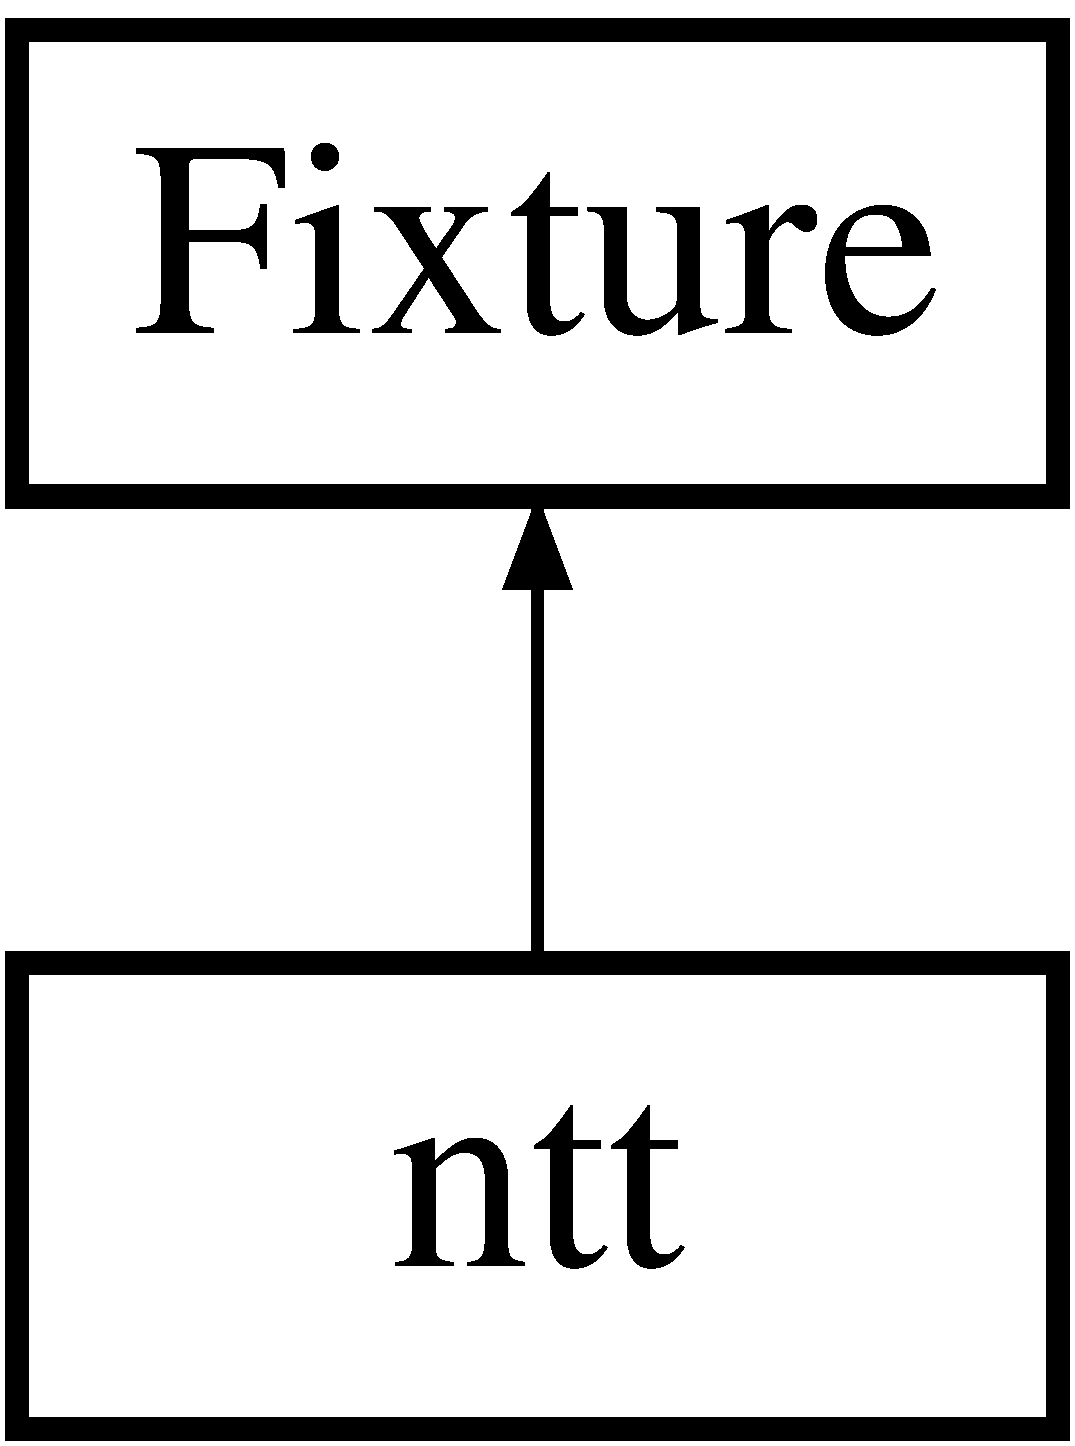
\includegraphics[height=2.000000cm]{classntt}
\end{center}
\end{figure}
\subsection*{Public Member Functions}
\begin{DoxyCompactItemize}
\item 
void \hyperlink{classntt_a733caaea7d6337e00168d78890b1cc37}{load\-\_\-ntt\-\_\-data} (size\-\_\-t work\-\_\-size)
\item 
void \hyperlink{classntt_a3ad95666ae0650b7022e7e695fa3ed28}{fpga\-\_\-ntt\-\_\-test} (size\-\_\-t work\-\_\-size)
\end{DoxyCompactItemize}


\subsection{Member Function Documentation}
\hypertarget{classntt_a3ad95666ae0650b7022e7e695fa3ed28}{\index{ntt@{ntt}!fpga\-\_\-ntt\-\_\-test@{fpga\-\_\-ntt\-\_\-test}}
\index{fpga\-\_\-ntt\-\_\-test@{fpga\-\_\-ntt\-\_\-test}!ntt@{ntt}}
\subsubsection[{fpga\-\_\-ntt\-\_\-test}]{\setlength{\rightskip}{0pt plus 5cm}void ntt\-::fpga\-\_\-ntt\-\_\-test (
\begin{DoxyParamCaption}
\item[{size\-\_\-t}]{work\-\_\-size}
\end{DoxyParamCaption}
)}}\label{classntt_a3ad95666ae0650b7022e7e695fa3ed28}
\hypertarget{classntt_a733caaea7d6337e00168d78890b1cc37}{\index{ntt@{ntt}!load\-\_\-ntt\-\_\-data@{load\-\_\-ntt\-\_\-data}}
\index{load\-\_\-ntt\-\_\-data@{load\-\_\-ntt\-\_\-data}!ntt@{ntt}}
\subsubsection[{load\-\_\-ntt\-\_\-data}]{\setlength{\rightskip}{0pt plus 5cm}void ntt\-::load\-\_\-ntt\-\_\-data (
\begin{DoxyParamCaption}
\item[{size\-\_\-t}]{work\-\_\-size}
\end{DoxyParamCaption}
)}}\label{classntt_a733caaea7d6337e00168d78890b1cc37}


The documentation for this class was generated from the following file\-:\begin{DoxyCompactItemize}
\item 
\hyperlink{bench__fwd__ntt_8cpp}{bench\-\_\-fwd\-\_\-ntt.\-cpp}\end{DoxyCompactItemize}

\hypertarget{classhetest_1_1utils_1_1NTT_1_1NTTImpl}{\section{hetest\-:\-:utils\-:\-:N\-T\-T\-:\-:N\-T\-T\-Impl Class Reference}
\label{classhetest_1_1utils_1_1NTT_1_1NTTImpl}\index{hetest\-::utils\-::\-N\-T\-T\-::\-N\-T\-T\-Impl@{hetest\-::utils\-::\-N\-T\-T\-::\-N\-T\-T\-Impl}}
}


{\ttfamily \#include $<$ntt.\-hpp$>$}

\subsection*{Public Member Functions}
\begin{DoxyCompactItemize}
\item 
\hyperlink{classhetest_1_1utils_1_1NTT_1_1NTTImpl_a44a582a60a18e2231deab0930f172aca}{N\-T\-T\-Impl} (uint64\-\_\-t degree, uint64\-\_\-t q, uint64\-\_\-t root\-\_\-of\-\_\-unity, std\-::shared\-\_\-ptr$<$ \hyperlink{structhetest_1_1utils_1_1AllocatorBase}{Allocator\-Base} $>$ alloc\-\_\-ptr=\{\})
\item 
\hyperlink{classhetest_1_1utils_1_1NTT_1_1NTTImpl_a7b480345b15a13da644d17463a7e7c16}{N\-T\-T\-Impl} (uint64\-\_\-t degree, uint64\-\_\-t q, std\-::shared\-\_\-ptr$<$ \hyperlink{structhetest_1_1utils_1_1AllocatorBase}{Allocator\-Base} $>$ alloc\-\_\-ptr=\{\})
\item 
\hyperlink{classhetest_1_1utils_1_1NTT_1_1NTTImpl_aeb47f4652bcb227cc5313db35a90ec8e}{$\sim$\-N\-T\-T\-Impl} ()
\item 
uint64\-\_\-t \hyperlink{classhetest_1_1utils_1_1NTT_1_1NTTImpl_aab44369dc7690791845a12bc35587157}{Get\-Minimal\-Root\-Of\-Unity} () const 
\item 
uint64\-\_\-t \hyperlink{classhetest_1_1utils_1_1NTT_1_1NTTImpl_a035d8b09e911d41bb5cde863aa5ad128}{Get\-Degree} () const 
\item 
uint64\-\_\-t \hyperlink{classhetest_1_1utils_1_1NTT_1_1NTTImpl_a4d2dac7a361d9afc6cee579d7322bd46}{Get\-Modulus} () const 
\item 
\hyperlink{namespacehetest_1_1utils_ad5b6a78d49dc8f6790f7fd2b10bf3db0}{Aligned\-Vector64}$<$ uint64\-\_\-t $>$ \& \hyperlink{classhetest_1_1utils_1_1NTT_1_1NTTImpl_aac30a427ad979f9b034bb04cbd6d8f27}{Get\-Precon64\-Root\-Of\-Unity\-Powers} ()
\item 
uint64\-\_\-t $\ast$ \hyperlink{classhetest_1_1utils_1_1NTT_1_1NTTImpl_ab534576b83c9c148ca285f304a5a4251}{Get\-Precon64\-Root\-Of\-Unity\-Powers\-Ptr} ()
\item 
\hyperlink{namespacehetest_1_1utils_ad5b6a78d49dc8f6790f7fd2b10bf3db0}{Aligned\-Vector64}$<$ uint64\-\_\-t $>$ \& \hyperlink{classhetest_1_1utils_1_1NTT_1_1NTTImpl_a1d155bcada1c332280941f5e082319a6}{Get\-Precon52\-Root\-Of\-Unity\-Powers} ()
\item 
uint64\-\_\-t $\ast$ \hyperlink{classhetest_1_1utils_1_1NTT_1_1NTTImpl_a7c77eaeda15cabc6d3c2868ff796b79f}{Get\-Precon52\-Root\-Of\-Unity\-Powers\-Ptr} ()
\item 
uint64\-\_\-t $\ast$ \hyperlink{classhetest_1_1utils_1_1NTT_1_1NTTImpl_a1f6d65ead7d22cbec7f985d6a9575ae6}{Get\-Root\-Of\-Unity\-Powers\-Ptr} ()
\item 
\hyperlink{namespacehetest_1_1utils_ad5b6a78d49dc8f6790f7fd2b10bf3db0}{Aligned\-Vector64}$<$ uint64\-\_\-t $>$ \& \hyperlink{classhetest_1_1utils_1_1NTT_1_1NTTImpl_a000757a957e7f530a4aa65018e2c3406}{Get\-Root\-Of\-Unity\-Powers} ()
\item 
uint64\-\_\-t \hyperlink{classhetest_1_1utils_1_1NTT_1_1NTTImpl_adc89766c94e7c6dd13d08d712daec265}{Get\-Root\-Of\-Unity\-Power} (size\-\_\-t i)
\item 
\hyperlink{namespacehetest_1_1utils_ad5b6a78d49dc8f6790f7fd2b10bf3db0}{Aligned\-Vector64}$<$ uint64\-\_\-t $>$ \& \hyperlink{classhetest_1_1utils_1_1NTT_1_1NTTImpl_a7b051fcc87e3f6f6df01b0d55e462777}{Get\-Precon64\-Inv\-Root\-Of\-Unity\-Powers} ()
\item 
uint64\-\_\-t $\ast$ \hyperlink{classhetest_1_1utils_1_1NTT_1_1NTTImpl_a04d04b88f14f5e79e5fb529f624559a1}{Get\-Precon64\-Inv\-Root\-Of\-Unity\-Powers\-Ptr} ()
\item 
\hyperlink{namespacehetest_1_1utils_ad5b6a78d49dc8f6790f7fd2b10bf3db0}{Aligned\-Vector64}$<$ uint64\-\_\-t $>$ \& \hyperlink{classhetest_1_1utils_1_1NTT_1_1NTTImpl_a60f96251a7f9f4876fa5a551cd4c894e}{Get\-Precon52\-Inv\-Root\-Of\-Unity\-Powers} ()
\item 
uint64\-\_\-t $\ast$ \hyperlink{classhetest_1_1utils_1_1NTT_1_1NTTImpl_af1bff60ad77232663df6c504b15cbe14}{Get\-Precon52\-Inv\-Root\-Of\-Unity\-Powers\-Ptr} ()
\item 
\hyperlink{namespacehetest_1_1utils_ad5b6a78d49dc8f6790f7fd2b10bf3db0}{Aligned\-Vector64}$<$ uint64\-\_\-t $>$ \& \hyperlink{classhetest_1_1utils_1_1NTT_1_1NTTImpl_a2afafd91a75934c0b004fcacb52506d0}{Get\-Inv\-Root\-Of\-Unity\-Powers} ()
\item 
uint64\-\_\-t $\ast$ \hyperlink{classhetest_1_1utils_1_1NTT_1_1NTTImpl_a2eb4f6dc13583dfa039aff9c86090b8b}{Get\-Inv\-Root\-Of\-Unity\-Powers\-Ptr} ()
\item 
uint64\-\_\-t \hyperlink{classhetest_1_1utils_1_1NTT_1_1NTTImpl_ae321a809bd4a9121b4d0a9a3c8f22851}{Get\-Inv\-Root\-Of\-Unity\-Power} (size\-\_\-t i)
\item 
void \hyperlink{classhetest_1_1utils_1_1NTT_1_1NTTImpl_a23e8a1b8cd8f2a3700b9daa7d729dcfc}{Compute\-Forward} (uint64\-\_\-t $\ast$result, const uint64\-\_\-t $\ast$operand, uint64\-\_\-t input\-\_\-mod\-\_\-factor, uint64\-\_\-t output\-\_\-mod\-\_\-factor)
\item 
void \hyperlink{classhetest_1_1utils_1_1NTT_1_1NTTImpl_aa9ddcd3bcd21f49f7c299959aae6baeb}{Compute\-Inverse} (uint64\-\_\-t $\ast$result, const uint64\-\_\-t $\ast$operand, uint64\-\_\-t input\-\_\-mod\-\_\-factor, uint64\-\_\-t output\-\_\-mod\-\_\-factor)
\end{DoxyCompactItemize}
\subsection*{Static Public Attributes}
\begin{DoxyCompactItemize}
\item 
static const size\-\_\-t \hyperlink{classhetest_1_1utils_1_1NTT_1_1NTTImpl_a44a2ac7f296bce27f708fb2e66ee1e5a}{s\-\_\-max\-\_\-degree\-\_\-bits} \{20\}
\item 
static const size\-\_\-t \hyperlink{classhetest_1_1utils_1_1NTT_1_1NTTImpl_ad457af43716b631a2471415bc604a530}{s\-\_\-max\-\_\-modulus\-\_\-bits} \{62\}
\item 
static const size\-\_\-t \hyperlink{classhetest_1_1utils_1_1NTT_1_1NTTImpl_a326fa5e71930b879eb060bc39ddd8d76}{s\-\_\-default\-\_\-shift\-\_\-bits} \{64\}
\item 
static const size\-\_\-t \hyperlink{classhetest_1_1utils_1_1NTT_1_1NTTImpl_a62363392951d4f7e9f380c4d427bef4b}{s\-\_\-ifma\-\_\-shift\-\_\-bits} \{52\}
\item 
static const size\-\_\-t \hyperlink{classhetest_1_1utils_1_1NTT_1_1NTTImpl_a7298cbc8ef00280200ac1bb1f416ca9a}{s\-\_\-max\-\_\-fwd\-\_\-ifma\-\_\-modulus} \{1\-U\-L\-L $<$$<$ (s\-\_\-ifma\-\_\-shift\-\_\-bits -\/ 2)\}
\item 
static const size\-\_\-t \hyperlink{classhetest_1_1utils_1_1NTT_1_1NTTImpl_adb491e973c3b2e087cc7ad5759fb6de4}{s\-\_\-max\-\_\-inv\-\_\-ifma\-\_\-modulus} \{1\-U\-L\-L $<$$<$ (s\-\_\-ifma\-\_\-shift\-\_\-bits -\/ 1)\}
\end{DoxyCompactItemize}


\subsection{Constructor \& Destructor Documentation}
\hypertarget{classhetest_1_1utils_1_1NTT_1_1NTTImpl_a44a582a60a18e2231deab0930f172aca}{\index{hetest\-::utils\-::\-N\-T\-T\-::\-N\-T\-T\-Impl@{hetest\-::utils\-::\-N\-T\-T\-::\-N\-T\-T\-Impl}!N\-T\-T\-Impl@{N\-T\-T\-Impl}}
\index{N\-T\-T\-Impl@{N\-T\-T\-Impl}!hetest::utils::NTT::NTTImpl@{hetest\-::utils\-::\-N\-T\-T\-::\-N\-T\-T\-Impl}}
\subsubsection[{N\-T\-T\-Impl}]{\setlength{\rightskip}{0pt plus 5cm}hetest\-::utils\-::\-N\-T\-T\-::\-N\-T\-T\-Impl\-::\-N\-T\-T\-Impl (
\begin{DoxyParamCaption}
\item[{uint64\-\_\-t}]{degree, }
\item[{uint64\-\_\-t}]{q, }
\item[{uint64\-\_\-t}]{root\-\_\-of\-\_\-unity, }
\item[{std\-::shared\-\_\-ptr$<$ {\bf Allocator\-Base} $>$}]{alloc\-\_\-ptr = {\ttfamily \{\}}}
\end{DoxyParamCaption}
)}}\label{classhetest_1_1utils_1_1NTT_1_1NTTImpl_a44a582a60a18e2231deab0930f172aca}
\hypertarget{classhetest_1_1utils_1_1NTT_1_1NTTImpl_a7b480345b15a13da644d17463a7e7c16}{\index{hetest\-::utils\-::\-N\-T\-T\-::\-N\-T\-T\-Impl@{hetest\-::utils\-::\-N\-T\-T\-::\-N\-T\-T\-Impl}!N\-T\-T\-Impl@{N\-T\-T\-Impl}}
\index{N\-T\-T\-Impl@{N\-T\-T\-Impl}!hetest::utils::NTT::NTTImpl@{hetest\-::utils\-::\-N\-T\-T\-::\-N\-T\-T\-Impl}}
\subsubsection[{N\-T\-T\-Impl}]{\setlength{\rightskip}{0pt plus 5cm}hetest\-::utils\-::\-N\-T\-T\-::\-N\-T\-T\-Impl\-::\-N\-T\-T\-Impl (
\begin{DoxyParamCaption}
\item[{uint64\-\_\-t}]{degree, }
\item[{uint64\-\_\-t}]{q, }
\item[{std\-::shared\-\_\-ptr$<$ {\bf Allocator\-Base} $>$}]{alloc\-\_\-ptr = {\ttfamily \{\}}}
\end{DoxyParamCaption}
)}}\label{classhetest_1_1utils_1_1NTT_1_1NTTImpl_a7b480345b15a13da644d17463a7e7c16}
\hypertarget{classhetest_1_1utils_1_1NTT_1_1NTTImpl_aeb47f4652bcb227cc5313db35a90ec8e}{\index{hetest\-::utils\-::\-N\-T\-T\-::\-N\-T\-T\-Impl@{hetest\-::utils\-::\-N\-T\-T\-::\-N\-T\-T\-Impl}!$\sim$\-N\-T\-T\-Impl@{$\sim$\-N\-T\-T\-Impl}}
\index{$\sim$\-N\-T\-T\-Impl@{$\sim$\-N\-T\-T\-Impl}!hetest::utils::NTT::NTTImpl@{hetest\-::utils\-::\-N\-T\-T\-::\-N\-T\-T\-Impl}}
\subsubsection[{$\sim$\-N\-T\-T\-Impl}]{\setlength{\rightskip}{0pt plus 5cm}hetest\-::utils\-::\-N\-T\-T\-::\-N\-T\-T\-Impl\-::$\sim$\-N\-T\-T\-Impl (
\begin{DoxyParamCaption}
{}
\end{DoxyParamCaption}
)\hspace{0.3cm}{\ttfamily [default]}}}\label{classhetest_1_1utils_1_1NTT_1_1NTTImpl_aeb47f4652bcb227cc5313db35a90ec8e}


\subsection{Member Function Documentation}
\hypertarget{classhetest_1_1utils_1_1NTT_1_1NTTImpl_a23e8a1b8cd8f2a3700b9daa7d729dcfc}{\index{hetest\-::utils\-::\-N\-T\-T\-::\-N\-T\-T\-Impl@{hetest\-::utils\-::\-N\-T\-T\-::\-N\-T\-T\-Impl}!Compute\-Forward@{Compute\-Forward}}
\index{Compute\-Forward@{Compute\-Forward}!hetest::utils::NTT::NTTImpl@{hetest\-::utils\-::\-N\-T\-T\-::\-N\-T\-T\-Impl}}
\subsubsection[{Compute\-Forward}]{\setlength{\rightskip}{0pt plus 5cm}void hetest\-::utils\-::\-N\-T\-T\-::\-N\-T\-T\-Impl\-::\-Compute\-Forward (
\begin{DoxyParamCaption}
\item[{uint64\-\_\-t $\ast$}]{result, }
\item[{const uint64\-\_\-t $\ast$}]{operand, }
\item[{uint64\-\_\-t}]{input\-\_\-mod\-\_\-factor, }
\item[{uint64\-\_\-t}]{output\-\_\-mod\-\_\-factor}
\end{DoxyParamCaption}
)}}\label{classhetest_1_1utils_1_1NTT_1_1NTTImpl_a23e8a1b8cd8f2a3700b9daa7d729dcfc}
\hypertarget{classhetest_1_1utils_1_1NTT_1_1NTTImpl_aa9ddcd3bcd21f49f7c299959aae6baeb}{\index{hetest\-::utils\-::\-N\-T\-T\-::\-N\-T\-T\-Impl@{hetest\-::utils\-::\-N\-T\-T\-::\-N\-T\-T\-Impl}!Compute\-Inverse@{Compute\-Inverse}}
\index{Compute\-Inverse@{Compute\-Inverse}!hetest::utils::NTT::NTTImpl@{hetest\-::utils\-::\-N\-T\-T\-::\-N\-T\-T\-Impl}}
\subsubsection[{Compute\-Inverse}]{\setlength{\rightskip}{0pt plus 5cm}void hetest\-::utils\-::\-N\-T\-T\-::\-N\-T\-T\-Impl\-::\-Compute\-Inverse (
\begin{DoxyParamCaption}
\item[{uint64\-\_\-t $\ast$}]{result, }
\item[{const uint64\-\_\-t $\ast$}]{operand, }
\item[{uint64\-\_\-t}]{input\-\_\-mod\-\_\-factor, }
\item[{uint64\-\_\-t}]{output\-\_\-mod\-\_\-factor}
\end{DoxyParamCaption}
)}}\label{classhetest_1_1utils_1_1NTT_1_1NTTImpl_aa9ddcd3bcd21f49f7c299959aae6baeb}
\hypertarget{classhetest_1_1utils_1_1NTT_1_1NTTImpl_a035d8b09e911d41bb5cde863aa5ad128}{\index{hetest\-::utils\-::\-N\-T\-T\-::\-N\-T\-T\-Impl@{hetest\-::utils\-::\-N\-T\-T\-::\-N\-T\-T\-Impl}!Get\-Degree@{Get\-Degree}}
\index{Get\-Degree@{Get\-Degree}!hetest::utils::NTT::NTTImpl@{hetest\-::utils\-::\-N\-T\-T\-::\-N\-T\-T\-Impl}}
\subsubsection[{Get\-Degree}]{\setlength{\rightskip}{0pt plus 5cm}uint64\-\_\-t hetest\-::utils\-::\-N\-T\-T\-::\-N\-T\-T\-Impl\-::\-Get\-Degree (
\begin{DoxyParamCaption}
{}
\end{DoxyParamCaption}
) const\hspace{0.3cm}{\ttfamily [inline]}}}\label{classhetest_1_1utils_1_1NTT_1_1NTTImpl_a035d8b09e911d41bb5cde863aa5ad128}
\hypertarget{classhetest_1_1utils_1_1NTT_1_1NTTImpl_ae321a809bd4a9121b4d0a9a3c8f22851}{\index{hetest\-::utils\-::\-N\-T\-T\-::\-N\-T\-T\-Impl@{hetest\-::utils\-::\-N\-T\-T\-::\-N\-T\-T\-Impl}!Get\-Inv\-Root\-Of\-Unity\-Power@{Get\-Inv\-Root\-Of\-Unity\-Power}}
\index{Get\-Inv\-Root\-Of\-Unity\-Power@{Get\-Inv\-Root\-Of\-Unity\-Power}!hetest::utils::NTT::NTTImpl@{hetest\-::utils\-::\-N\-T\-T\-::\-N\-T\-T\-Impl}}
\subsubsection[{Get\-Inv\-Root\-Of\-Unity\-Power}]{\setlength{\rightskip}{0pt plus 5cm}uint64\-\_\-t hetest\-::utils\-::\-N\-T\-T\-::\-N\-T\-T\-Impl\-::\-Get\-Inv\-Root\-Of\-Unity\-Power (
\begin{DoxyParamCaption}
\item[{size\-\_\-t}]{i}
\end{DoxyParamCaption}
)\hspace{0.3cm}{\ttfamily [inline]}}}\label{classhetest_1_1utils_1_1NTT_1_1NTTImpl_ae321a809bd4a9121b4d0a9a3c8f22851}
\hypertarget{classhetest_1_1utils_1_1NTT_1_1NTTImpl_a2afafd91a75934c0b004fcacb52506d0}{\index{hetest\-::utils\-::\-N\-T\-T\-::\-N\-T\-T\-Impl@{hetest\-::utils\-::\-N\-T\-T\-::\-N\-T\-T\-Impl}!Get\-Inv\-Root\-Of\-Unity\-Powers@{Get\-Inv\-Root\-Of\-Unity\-Powers}}
\index{Get\-Inv\-Root\-Of\-Unity\-Powers@{Get\-Inv\-Root\-Of\-Unity\-Powers}!hetest::utils::NTT::NTTImpl@{hetest\-::utils\-::\-N\-T\-T\-::\-N\-T\-T\-Impl}}
\subsubsection[{Get\-Inv\-Root\-Of\-Unity\-Powers}]{\setlength{\rightskip}{0pt plus 5cm}{\bf Aligned\-Vector64}$<$uint64\-\_\-t$>$\& hetest\-::utils\-::\-N\-T\-T\-::\-N\-T\-T\-Impl\-::\-Get\-Inv\-Root\-Of\-Unity\-Powers (
\begin{DoxyParamCaption}
{}
\end{DoxyParamCaption}
)\hspace{0.3cm}{\ttfamily [inline]}}}\label{classhetest_1_1utils_1_1NTT_1_1NTTImpl_a2afafd91a75934c0b004fcacb52506d0}
\hypertarget{classhetest_1_1utils_1_1NTT_1_1NTTImpl_a2eb4f6dc13583dfa039aff9c86090b8b}{\index{hetest\-::utils\-::\-N\-T\-T\-::\-N\-T\-T\-Impl@{hetest\-::utils\-::\-N\-T\-T\-::\-N\-T\-T\-Impl}!Get\-Inv\-Root\-Of\-Unity\-Powers\-Ptr@{Get\-Inv\-Root\-Of\-Unity\-Powers\-Ptr}}
\index{Get\-Inv\-Root\-Of\-Unity\-Powers\-Ptr@{Get\-Inv\-Root\-Of\-Unity\-Powers\-Ptr}!hetest::utils::NTT::NTTImpl@{hetest\-::utils\-::\-N\-T\-T\-::\-N\-T\-T\-Impl}}
\subsubsection[{Get\-Inv\-Root\-Of\-Unity\-Powers\-Ptr}]{\setlength{\rightskip}{0pt plus 5cm}uint64\-\_\-t$\ast$ hetest\-::utils\-::\-N\-T\-T\-::\-N\-T\-T\-Impl\-::\-Get\-Inv\-Root\-Of\-Unity\-Powers\-Ptr (
\begin{DoxyParamCaption}
{}
\end{DoxyParamCaption}
)\hspace{0.3cm}{\ttfamily [inline]}}}\label{classhetest_1_1utils_1_1NTT_1_1NTTImpl_a2eb4f6dc13583dfa039aff9c86090b8b}
\hypertarget{classhetest_1_1utils_1_1NTT_1_1NTTImpl_aab44369dc7690791845a12bc35587157}{\index{hetest\-::utils\-::\-N\-T\-T\-::\-N\-T\-T\-Impl@{hetest\-::utils\-::\-N\-T\-T\-::\-N\-T\-T\-Impl}!Get\-Minimal\-Root\-Of\-Unity@{Get\-Minimal\-Root\-Of\-Unity}}
\index{Get\-Minimal\-Root\-Of\-Unity@{Get\-Minimal\-Root\-Of\-Unity}!hetest::utils::NTT::NTTImpl@{hetest\-::utils\-::\-N\-T\-T\-::\-N\-T\-T\-Impl}}
\subsubsection[{Get\-Minimal\-Root\-Of\-Unity}]{\setlength{\rightskip}{0pt plus 5cm}uint64\-\_\-t hetest\-::utils\-::\-N\-T\-T\-::\-N\-T\-T\-Impl\-::\-Get\-Minimal\-Root\-Of\-Unity (
\begin{DoxyParamCaption}
{}
\end{DoxyParamCaption}
) const\hspace{0.3cm}{\ttfamily [inline]}}}\label{classhetest_1_1utils_1_1NTT_1_1NTTImpl_aab44369dc7690791845a12bc35587157}
\hypertarget{classhetest_1_1utils_1_1NTT_1_1NTTImpl_a4d2dac7a361d9afc6cee579d7322bd46}{\index{hetest\-::utils\-::\-N\-T\-T\-::\-N\-T\-T\-Impl@{hetest\-::utils\-::\-N\-T\-T\-::\-N\-T\-T\-Impl}!Get\-Modulus@{Get\-Modulus}}
\index{Get\-Modulus@{Get\-Modulus}!hetest::utils::NTT::NTTImpl@{hetest\-::utils\-::\-N\-T\-T\-::\-N\-T\-T\-Impl}}
\subsubsection[{Get\-Modulus}]{\setlength{\rightskip}{0pt plus 5cm}uint64\-\_\-t hetest\-::utils\-::\-N\-T\-T\-::\-N\-T\-T\-Impl\-::\-Get\-Modulus (
\begin{DoxyParamCaption}
{}
\end{DoxyParamCaption}
) const\hspace{0.3cm}{\ttfamily [inline]}}}\label{classhetest_1_1utils_1_1NTT_1_1NTTImpl_a4d2dac7a361d9afc6cee579d7322bd46}
\hypertarget{classhetest_1_1utils_1_1NTT_1_1NTTImpl_a60f96251a7f9f4876fa5a551cd4c894e}{\index{hetest\-::utils\-::\-N\-T\-T\-::\-N\-T\-T\-Impl@{hetest\-::utils\-::\-N\-T\-T\-::\-N\-T\-T\-Impl}!Get\-Precon52\-Inv\-Root\-Of\-Unity\-Powers@{Get\-Precon52\-Inv\-Root\-Of\-Unity\-Powers}}
\index{Get\-Precon52\-Inv\-Root\-Of\-Unity\-Powers@{Get\-Precon52\-Inv\-Root\-Of\-Unity\-Powers}!hetest::utils::NTT::NTTImpl@{hetest\-::utils\-::\-N\-T\-T\-::\-N\-T\-T\-Impl}}
\subsubsection[{Get\-Precon52\-Inv\-Root\-Of\-Unity\-Powers}]{\setlength{\rightskip}{0pt plus 5cm}{\bf Aligned\-Vector64}$<$uint64\-\_\-t$>$\& hetest\-::utils\-::\-N\-T\-T\-::\-N\-T\-T\-Impl\-::\-Get\-Precon52\-Inv\-Root\-Of\-Unity\-Powers (
\begin{DoxyParamCaption}
{}
\end{DoxyParamCaption}
)\hspace{0.3cm}{\ttfamily [inline]}}}\label{classhetest_1_1utils_1_1NTT_1_1NTTImpl_a60f96251a7f9f4876fa5a551cd4c894e}
\hypertarget{classhetest_1_1utils_1_1NTT_1_1NTTImpl_af1bff60ad77232663df6c504b15cbe14}{\index{hetest\-::utils\-::\-N\-T\-T\-::\-N\-T\-T\-Impl@{hetest\-::utils\-::\-N\-T\-T\-::\-N\-T\-T\-Impl}!Get\-Precon52\-Inv\-Root\-Of\-Unity\-Powers\-Ptr@{Get\-Precon52\-Inv\-Root\-Of\-Unity\-Powers\-Ptr}}
\index{Get\-Precon52\-Inv\-Root\-Of\-Unity\-Powers\-Ptr@{Get\-Precon52\-Inv\-Root\-Of\-Unity\-Powers\-Ptr}!hetest::utils::NTT::NTTImpl@{hetest\-::utils\-::\-N\-T\-T\-::\-N\-T\-T\-Impl}}
\subsubsection[{Get\-Precon52\-Inv\-Root\-Of\-Unity\-Powers\-Ptr}]{\setlength{\rightskip}{0pt plus 5cm}uint64\-\_\-t$\ast$ hetest\-::utils\-::\-N\-T\-T\-::\-N\-T\-T\-Impl\-::\-Get\-Precon52\-Inv\-Root\-Of\-Unity\-Powers\-Ptr (
\begin{DoxyParamCaption}
{}
\end{DoxyParamCaption}
)\hspace{0.3cm}{\ttfamily [inline]}}}\label{classhetest_1_1utils_1_1NTT_1_1NTTImpl_af1bff60ad77232663df6c504b15cbe14}
\hypertarget{classhetest_1_1utils_1_1NTT_1_1NTTImpl_a1d155bcada1c332280941f5e082319a6}{\index{hetest\-::utils\-::\-N\-T\-T\-::\-N\-T\-T\-Impl@{hetest\-::utils\-::\-N\-T\-T\-::\-N\-T\-T\-Impl}!Get\-Precon52\-Root\-Of\-Unity\-Powers@{Get\-Precon52\-Root\-Of\-Unity\-Powers}}
\index{Get\-Precon52\-Root\-Of\-Unity\-Powers@{Get\-Precon52\-Root\-Of\-Unity\-Powers}!hetest::utils::NTT::NTTImpl@{hetest\-::utils\-::\-N\-T\-T\-::\-N\-T\-T\-Impl}}
\subsubsection[{Get\-Precon52\-Root\-Of\-Unity\-Powers}]{\setlength{\rightskip}{0pt plus 5cm}{\bf Aligned\-Vector64}$<$uint64\-\_\-t$>$\& hetest\-::utils\-::\-N\-T\-T\-::\-N\-T\-T\-Impl\-::\-Get\-Precon52\-Root\-Of\-Unity\-Powers (
\begin{DoxyParamCaption}
{}
\end{DoxyParamCaption}
)\hspace{0.3cm}{\ttfamily [inline]}}}\label{classhetest_1_1utils_1_1NTT_1_1NTTImpl_a1d155bcada1c332280941f5e082319a6}
\hypertarget{classhetest_1_1utils_1_1NTT_1_1NTTImpl_a7c77eaeda15cabc6d3c2868ff796b79f}{\index{hetest\-::utils\-::\-N\-T\-T\-::\-N\-T\-T\-Impl@{hetest\-::utils\-::\-N\-T\-T\-::\-N\-T\-T\-Impl}!Get\-Precon52\-Root\-Of\-Unity\-Powers\-Ptr@{Get\-Precon52\-Root\-Of\-Unity\-Powers\-Ptr}}
\index{Get\-Precon52\-Root\-Of\-Unity\-Powers\-Ptr@{Get\-Precon52\-Root\-Of\-Unity\-Powers\-Ptr}!hetest::utils::NTT::NTTImpl@{hetest\-::utils\-::\-N\-T\-T\-::\-N\-T\-T\-Impl}}
\subsubsection[{Get\-Precon52\-Root\-Of\-Unity\-Powers\-Ptr}]{\setlength{\rightskip}{0pt plus 5cm}uint64\-\_\-t$\ast$ hetest\-::utils\-::\-N\-T\-T\-::\-N\-T\-T\-Impl\-::\-Get\-Precon52\-Root\-Of\-Unity\-Powers\-Ptr (
\begin{DoxyParamCaption}
{}
\end{DoxyParamCaption}
)\hspace{0.3cm}{\ttfamily [inline]}}}\label{classhetest_1_1utils_1_1NTT_1_1NTTImpl_a7c77eaeda15cabc6d3c2868ff796b79f}
\hypertarget{classhetest_1_1utils_1_1NTT_1_1NTTImpl_a7b051fcc87e3f6f6df01b0d55e462777}{\index{hetest\-::utils\-::\-N\-T\-T\-::\-N\-T\-T\-Impl@{hetest\-::utils\-::\-N\-T\-T\-::\-N\-T\-T\-Impl}!Get\-Precon64\-Inv\-Root\-Of\-Unity\-Powers@{Get\-Precon64\-Inv\-Root\-Of\-Unity\-Powers}}
\index{Get\-Precon64\-Inv\-Root\-Of\-Unity\-Powers@{Get\-Precon64\-Inv\-Root\-Of\-Unity\-Powers}!hetest::utils::NTT::NTTImpl@{hetest\-::utils\-::\-N\-T\-T\-::\-N\-T\-T\-Impl}}
\subsubsection[{Get\-Precon64\-Inv\-Root\-Of\-Unity\-Powers}]{\setlength{\rightskip}{0pt plus 5cm}{\bf Aligned\-Vector64}$<$uint64\-\_\-t$>$\& hetest\-::utils\-::\-N\-T\-T\-::\-N\-T\-T\-Impl\-::\-Get\-Precon64\-Inv\-Root\-Of\-Unity\-Powers (
\begin{DoxyParamCaption}
{}
\end{DoxyParamCaption}
)\hspace{0.3cm}{\ttfamily [inline]}}}\label{classhetest_1_1utils_1_1NTT_1_1NTTImpl_a7b051fcc87e3f6f6df01b0d55e462777}
\hypertarget{classhetest_1_1utils_1_1NTT_1_1NTTImpl_a04d04b88f14f5e79e5fb529f624559a1}{\index{hetest\-::utils\-::\-N\-T\-T\-::\-N\-T\-T\-Impl@{hetest\-::utils\-::\-N\-T\-T\-::\-N\-T\-T\-Impl}!Get\-Precon64\-Inv\-Root\-Of\-Unity\-Powers\-Ptr@{Get\-Precon64\-Inv\-Root\-Of\-Unity\-Powers\-Ptr}}
\index{Get\-Precon64\-Inv\-Root\-Of\-Unity\-Powers\-Ptr@{Get\-Precon64\-Inv\-Root\-Of\-Unity\-Powers\-Ptr}!hetest::utils::NTT::NTTImpl@{hetest\-::utils\-::\-N\-T\-T\-::\-N\-T\-T\-Impl}}
\subsubsection[{Get\-Precon64\-Inv\-Root\-Of\-Unity\-Powers\-Ptr}]{\setlength{\rightskip}{0pt plus 5cm}uint64\-\_\-t$\ast$ hetest\-::utils\-::\-N\-T\-T\-::\-N\-T\-T\-Impl\-::\-Get\-Precon64\-Inv\-Root\-Of\-Unity\-Powers\-Ptr (
\begin{DoxyParamCaption}
{}
\end{DoxyParamCaption}
)\hspace{0.3cm}{\ttfamily [inline]}}}\label{classhetest_1_1utils_1_1NTT_1_1NTTImpl_a04d04b88f14f5e79e5fb529f624559a1}
\hypertarget{classhetest_1_1utils_1_1NTT_1_1NTTImpl_aac30a427ad979f9b034bb04cbd6d8f27}{\index{hetest\-::utils\-::\-N\-T\-T\-::\-N\-T\-T\-Impl@{hetest\-::utils\-::\-N\-T\-T\-::\-N\-T\-T\-Impl}!Get\-Precon64\-Root\-Of\-Unity\-Powers@{Get\-Precon64\-Root\-Of\-Unity\-Powers}}
\index{Get\-Precon64\-Root\-Of\-Unity\-Powers@{Get\-Precon64\-Root\-Of\-Unity\-Powers}!hetest::utils::NTT::NTTImpl@{hetest\-::utils\-::\-N\-T\-T\-::\-N\-T\-T\-Impl}}
\subsubsection[{Get\-Precon64\-Root\-Of\-Unity\-Powers}]{\setlength{\rightskip}{0pt plus 5cm}{\bf Aligned\-Vector64}$<$uint64\-\_\-t$>$\& hetest\-::utils\-::\-N\-T\-T\-::\-N\-T\-T\-Impl\-::\-Get\-Precon64\-Root\-Of\-Unity\-Powers (
\begin{DoxyParamCaption}
{}
\end{DoxyParamCaption}
)\hspace{0.3cm}{\ttfamily [inline]}}}\label{classhetest_1_1utils_1_1NTT_1_1NTTImpl_aac30a427ad979f9b034bb04cbd6d8f27}
\hypertarget{classhetest_1_1utils_1_1NTT_1_1NTTImpl_ab534576b83c9c148ca285f304a5a4251}{\index{hetest\-::utils\-::\-N\-T\-T\-::\-N\-T\-T\-Impl@{hetest\-::utils\-::\-N\-T\-T\-::\-N\-T\-T\-Impl}!Get\-Precon64\-Root\-Of\-Unity\-Powers\-Ptr@{Get\-Precon64\-Root\-Of\-Unity\-Powers\-Ptr}}
\index{Get\-Precon64\-Root\-Of\-Unity\-Powers\-Ptr@{Get\-Precon64\-Root\-Of\-Unity\-Powers\-Ptr}!hetest::utils::NTT::NTTImpl@{hetest\-::utils\-::\-N\-T\-T\-::\-N\-T\-T\-Impl}}
\subsubsection[{Get\-Precon64\-Root\-Of\-Unity\-Powers\-Ptr}]{\setlength{\rightskip}{0pt plus 5cm}uint64\-\_\-t$\ast$ hetest\-::utils\-::\-N\-T\-T\-::\-N\-T\-T\-Impl\-::\-Get\-Precon64\-Root\-Of\-Unity\-Powers\-Ptr (
\begin{DoxyParamCaption}
{}
\end{DoxyParamCaption}
)\hspace{0.3cm}{\ttfamily [inline]}}}\label{classhetest_1_1utils_1_1NTT_1_1NTTImpl_ab534576b83c9c148ca285f304a5a4251}
\hypertarget{classhetest_1_1utils_1_1NTT_1_1NTTImpl_adc89766c94e7c6dd13d08d712daec265}{\index{hetest\-::utils\-::\-N\-T\-T\-::\-N\-T\-T\-Impl@{hetest\-::utils\-::\-N\-T\-T\-::\-N\-T\-T\-Impl}!Get\-Root\-Of\-Unity\-Power@{Get\-Root\-Of\-Unity\-Power}}
\index{Get\-Root\-Of\-Unity\-Power@{Get\-Root\-Of\-Unity\-Power}!hetest::utils::NTT::NTTImpl@{hetest\-::utils\-::\-N\-T\-T\-::\-N\-T\-T\-Impl}}
\subsubsection[{Get\-Root\-Of\-Unity\-Power}]{\setlength{\rightskip}{0pt plus 5cm}uint64\-\_\-t hetest\-::utils\-::\-N\-T\-T\-::\-N\-T\-T\-Impl\-::\-Get\-Root\-Of\-Unity\-Power (
\begin{DoxyParamCaption}
\item[{size\-\_\-t}]{i}
\end{DoxyParamCaption}
)\hspace{0.3cm}{\ttfamily [inline]}}}\label{classhetest_1_1utils_1_1NTT_1_1NTTImpl_adc89766c94e7c6dd13d08d712daec265}
\hypertarget{classhetest_1_1utils_1_1NTT_1_1NTTImpl_a000757a957e7f530a4aa65018e2c3406}{\index{hetest\-::utils\-::\-N\-T\-T\-::\-N\-T\-T\-Impl@{hetest\-::utils\-::\-N\-T\-T\-::\-N\-T\-T\-Impl}!Get\-Root\-Of\-Unity\-Powers@{Get\-Root\-Of\-Unity\-Powers}}
\index{Get\-Root\-Of\-Unity\-Powers@{Get\-Root\-Of\-Unity\-Powers}!hetest::utils::NTT::NTTImpl@{hetest\-::utils\-::\-N\-T\-T\-::\-N\-T\-T\-Impl}}
\subsubsection[{Get\-Root\-Of\-Unity\-Powers}]{\setlength{\rightskip}{0pt plus 5cm}{\bf Aligned\-Vector64}$<$uint64\-\_\-t$>$\& hetest\-::utils\-::\-N\-T\-T\-::\-N\-T\-T\-Impl\-::\-Get\-Root\-Of\-Unity\-Powers (
\begin{DoxyParamCaption}
{}
\end{DoxyParamCaption}
)\hspace{0.3cm}{\ttfamily [inline]}}}\label{classhetest_1_1utils_1_1NTT_1_1NTTImpl_a000757a957e7f530a4aa65018e2c3406}
\hypertarget{classhetest_1_1utils_1_1NTT_1_1NTTImpl_a1f6d65ead7d22cbec7f985d6a9575ae6}{\index{hetest\-::utils\-::\-N\-T\-T\-::\-N\-T\-T\-Impl@{hetest\-::utils\-::\-N\-T\-T\-::\-N\-T\-T\-Impl}!Get\-Root\-Of\-Unity\-Powers\-Ptr@{Get\-Root\-Of\-Unity\-Powers\-Ptr}}
\index{Get\-Root\-Of\-Unity\-Powers\-Ptr@{Get\-Root\-Of\-Unity\-Powers\-Ptr}!hetest::utils::NTT::NTTImpl@{hetest\-::utils\-::\-N\-T\-T\-::\-N\-T\-T\-Impl}}
\subsubsection[{Get\-Root\-Of\-Unity\-Powers\-Ptr}]{\setlength{\rightskip}{0pt plus 5cm}uint64\-\_\-t$\ast$ hetest\-::utils\-::\-N\-T\-T\-::\-N\-T\-T\-Impl\-::\-Get\-Root\-Of\-Unity\-Powers\-Ptr (
\begin{DoxyParamCaption}
{}
\end{DoxyParamCaption}
)\hspace{0.3cm}{\ttfamily [inline]}}}\label{classhetest_1_1utils_1_1NTT_1_1NTTImpl_a1f6d65ead7d22cbec7f985d6a9575ae6}


\subsection{Member Data Documentation}
\hypertarget{classhetest_1_1utils_1_1NTT_1_1NTTImpl_a326fa5e71930b879eb060bc39ddd8d76}{\index{hetest\-::utils\-::\-N\-T\-T\-::\-N\-T\-T\-Impl@{hetest\-::utils\-::\-N\-T\-T\-::\-N\-T\-T\-Impl}!s\-\_\-default\-\_\-shift\-\_\-bits@{s\-\_\-default\-\_\-shift\-\_\-bits}}
\index{s\-\_\-default\-\_\-shift\-\_\-bits@{s\-\_\-default\-\_\-shift\-\_\-bits}!hetest::utils::NTT::NTTImpl@{hetest\-::utils\-::\-N\-T\-T\-::\-N\-T\-T\-Impl}}
\subsubsection[{s\-\_\-default\-\_\-shift\-\_\-bits}]{\setlength{\rightskip}{0pt plus 5cm}const size\-\_\-t hetest\-::utils\-::\-N\-T\-T\-::\-N\-T\-T\-Impl\-::s\-\_\-default\-\_\-shift\-\_\-bits \{64\}\hspace{0.3cm}{\ttfamily [static]}}}\label{classhetest_1_1utils_1_1NTT_1_1NTTImpl_a326fa5e71930b879eb060bc39ddd8d76}
\hypertarget{classhetest_1_1utils_1_1NTT_1_1NTTImpl_a62363392951d4f7e9f380c4d427bef4b}{\index{hetest\-::utils\-::\-N\-T\-T\-::\-N\-T\-T\-Impl@{hetest\-::utils\-::\-N\-T\-T\-::\-N\-T\-T\-Impl}!s\-\_\-ifma\-\_\-shift\-\_\-bits@{s\-\_\-ifma\-\_\-shift\-\_\-bits}}
\index{s\-\_\-ifma\-\_\-shift\-\_\-bits@{s\-\_\-ifma\-\_\-shift\-\_\-bits}!hetest::utils::NTT::NTTImpl@{hetest\-::utils\-::\-N\-T\-T\-::\-N\-T\-T\-Impl}}
\subsubsection[{s\-\_\-ifma\-\_\-shift\-\_\-bits}]{\setlength{\rightskip}{0pt plus 5cm}const size\-\_\-t hetest\-::utils\-::\-N\-T\-T\-::\-N\-T\-T\-Impl\-::s\-\_\-ifma\-\_\-shift\-\_\-bits \{52\}\hspace{0.3cm}{\ttfamily [static]}}}\label{classhetest_1_1utils_1_1NTT_1_1NTTImpl_a62363392951d4f7e9f380c4d427bef4b}
\hypertarget{classhetest_1_1utils_1_1NTT_1_1NTTImpl_a44a2ac7f296bce27f708fb2e66ee1e5a}{\index{hetest\-::utils\-::\-N\-T\-T\-::\-N\-T\-T\-Impl@{hetest\-::utils\-::\-N\-T\-T\-::\-N\-T\-T\-Impl}!s\-\_\-max\-\_\-degree\-\_\-bits@{s\-\_\-max\-\_\-degree\-\_\-bits}}
\index{s\-\_\-max\-\_\-degree\-\_\-bits@{s\-\_\-max\-\_\-degree\-\_\-bits}!hetest::utils::NTT::NTTImpl@{hetest\-::utils\-::\-N\-T\-T\-::\-N\-T\-T\-Impl}}
\subsubsection[{s\-\_\-max\-\_\-degree\-\_\-bits}]{\setlength{\rightskip}{0pt plus 5cm}const size\-\_\-t hetest\-::utils\-::\-N\-T\-T\-::\-N\-T\-T\-Impl\-::s\-\_\-max\-\_\-degree\-\_\-bits \{20\}\hspace{0.3cm}{\ttfamily [static]}}}\label{classhetest_1_1utils_1_1NTT_1_1NTTImpl_a44a2ac7f296bce27f708fb2e66ee1e5a}
\hypertarget{classhetest_1_1utils_1_1NTT_1_1NTTImpl_a7298cbc8ef00280200ac1bb1f416ca9a}{\index{hetest\-::utils\-::\-N\-T\-T\-::\-N\-T\-T\-Impl@{hetest\-::utils\-::\-N\-T\-T\-::\-N\-T\-T\-Impl}!s\-\_\-max\-\_\-fwd\-\_\-ifma\-\_\-modulus@{s\-\_\-max\-\_\-fwd\-\_\-ifma\-\_\-modulus}}
\index{s\-\_\-max\-\_\-fwd\-\_\-ifma\-\_\-modulus@{s\-\_\-max\-\_\-fwd\-\_\-ifma\-\_\-modulus}!hetest::utils::NTT::NTTImpl@{hetest\-::utils\-::\-N\-T\-T\-::\-N\-T\-T\-Impl}}
\subsubsection[{s\-\_\-max\-\_\-fwd\-\_\-ifma\-\_\-modulus}]{\setlength{\rightskip}{0pt plus 5cm}const size\-\_\-t hetest\-::utils\-::\-N\-T\-T\-::\-N\-T\-T\-Impl\-::s\-\_\-max\-\_\-fwd\-\_\-ifma\-\_\-modulus \{1\-U\-L\-L $<$$<$ (s\-\_\-ifma\-\_\-shift\-\_\-bits -\/ 2)\}\hspace{0.3cm}{\ttfamily [static]}}}\label{classhetest_1_1utils_1_1NTT_1_1NTTImpl_a7298cbc8ef00280200ac1bb1f416ca9a}
\hypertarget{classhetest_1_1utils_1_1NTT_1_1NTTImpl_adb491e973c3b2e087cc7ad5759fb6de4}{\index{hetest\-::utils\-::\-N\-T\-T\-::\-N\-T\-T\-Impl@{hetest\-::utils\-::\-N\-T\-T\-::\-N\-T\-T\-Impl}!s\-\_\-max\-\_\-inv\-\_\-ifma\-\_\-modulus@{s\-\_\-max\-\_\-inv\-\_\-ifma\-\_\-modulus}}
\index{s\-\_\-max\-\_\-inv\-\_\-ifma\-\_\-modulus@{s\-\_\-max\-\_\-inv\-\_\-ifma\-\_\-modulus}!hetest::utils::NTT::NTTImpl@{hetest\-::utils\-::\-N\-T\-T\-::\-N\-T\-T\-Impl}}
\subsubsection[{s\-\_\-max\-\_\-inv\-\_\-ifma\-\_\-modulus}]{\setlength{\rightskip}{0pt plus 5cm}const size\-\_\-t hetest\-::utils\-::\-N\-T\-T\-::\-N\-T\-T\-Impl\-::s\-\_\-max\-\_\-inv\-\_\-ifma\-\_\-modulus \{1\-U\-L\-L $<$$<$ (s\-\_\-ifma\-\_\-shift\-\_\-bits -\/ 1)\}\hspace{0.3cm}{\ttfamily [static]}}}\label{classhetest_1_1utils_1_1NTT_1_1NTTImpl_adb491e973c3b2e087cc7ad5759fb6de4}
\hypertarget{classhetest_1_1utils_1_1NTT_1_1NTTImpl_ad457af43716b631a2471415bc604a530}{\index{hetest\-::utils\-::\-N\-T\-T\-::\-N\-T\-T\-Impl@{hetest\-::utils\-::\-N\-T\-T\-::\-N\-T\-T\-Impl}!s\-\_\-max\-\_\-modulus\-\_\-bits@{s\-\_\-max\-\_\-modulus\-\_\-bits}}
\index{s\-\_\-max\-\_\-modulus\-\_\-bits@{s\-\_\-max\-\_\-modulus\-\_\-bits}!hetest::utils::NTT::NTTImpl@{hetest\-::utils\-::\-N\-T\-T\-::\-N\-T\-T\-Impl}}
\subsubsection[{s\-\_\-max\-\_\-modulus\-\_\-bits}]{\setlength{\rightskip}{0pt plus 5cm}const size\-\_\-t hetest\-::utils\-::\-N\-T\-T\-::\-N\-T\-T\-Impl\-::s\-\_\-max\-\_\-modulus\-\_\-bits \{62\}\hspace{0.3cm}{\ttfamily [static]}}}\label{classhetest_1_1utils_1_1NTT_1_1NTTImpl_ad457af43716b631a2471415bc604a530}


The documentation for this class was generated from the following files\-:\begin{DoxyCompactItemize}
\item 
\hyperlink{ntt_8hpp}{ntt.\-hpp}\item 
\hyperlink{ntt_8cpp}{ntt.\-cpp}\end{DoxyCompactItemize}

\hypertarget{structintel_1_1hexl_1_1fpga_1_1Object}{\section{intel\-:\-:hexl\-:\-:fpga\-:\-:Object Struct Reference}
\label{structintel_1_1hexl_1_1fpga_1_1Object}\index{intel\-::hexl\-::fpga\-::\-Object@{intel\-::hexl\-::fpga\-::\-Object}}
}


Struct \hyperlink{structintel_1_1hexl_1_1fpga_1_1Object}{Object}.  




{\ttfamily \#include $<$fpga.\-h$>$}

Inheritance diagram for intel\-:\-:hexl\-:\-:fpga\-:\-:Object\-:\begin{figure}[H]
\begin{center}
\leavevmode
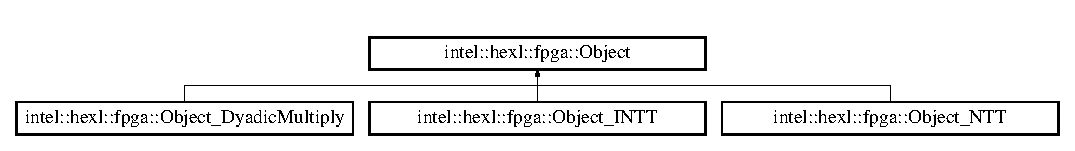
\includegraphics[height=1.181435cm]{structintel_1_1hexl_1_1fpga_1_1Object}
\end{center}
\end{figure}
\subsection*{Public Member Functions}
\begin{DoxyCompactItemize}
\item 
\hyperlink{structintel_1_1hexl_1_1fpga_1_1Object_afbecbde0e8e9f2e4b87326d164d2f3a6}{Object} (\hyperlink{namespaceintel_1_1hexl_1_1fpga_a9f07798cd59a71b9f57156192f7bf2f6}{kernel\-\_\-t} type=kernel\-\_\-t\-::\-N\-O\-N\-E, bool fence=false)
\item 
virtual \hyperlink{structintel_1_1hexl_1_1fpga_1_1Object_a53dd49a3d2fe50a55d91eda3f139e04f}{$\sim$\-Object} ()=default
\end{DoxyCompactItemize}
\subsection*{Public Attributes}
\begin{DoxyCompactItemize}
\item 
bool \hyperlink{structintel_1_1hexl_1_1fpga_1_1Object_a8d6495f3b68194f0c38927d76e9c652c}{ready\-\_\-}
\item 
int \hyperlink{structintel_1_1hexl_1_1fpga_1_1Object_ade9313d87b44bc1bfeccca2f5829ceae}{id\-\_\-}
\item 
\hyperlink{namespaceintel_1_1hexl_1_1fpga_a9f07798cd59a71b9f57156192f7bf2f6}{kernel\-\_\-t} \hyperlink{structintel_1_1hexl_1_1fpga_1_1Object_a795a35540ad7bb347d3978ca83f72e8b}{type\-\_\-}
\item 
bool \hyperlink{structintel_1_1hexl_1_1fpga_1_1Object_a187c9e1d3e7dca831390d438cee83b13}{fence\-\_\-}
\end{DoxyCompactItemize}
\subsection*{Static Public Attributes}
\begin{DoxyCompactItemize}
\item 
static unsigned int \hyperlink{structintel_1_1hexl_1_1fpga_1_1Object_a0da02feafb293ff8cea005f6312bd638}{g\-\_\-wid\-\_\-}
\end{DoxyCompactItemize}


\subsection{Detailed Description}
Struct \hyperlink{structintel_1_1hexl_1_1fpga_1_1Object}{Object}. 


\begin{DoxyParams}[1]{Parameters}
\mbox{\tt in}  & {\em modulus} & stores the polynomial modulus \\
\hline
\mbox{\tt in}  & {\em ready\-\_\-} & flag indicating that the \hyperlink{structintel_1_1hexl_1_1fpga_1_1Object}{Object} is ready for processing \\
\hline
\mbox{\tt in}  & {\em id\-\_\-} & \hyperlink{structintel_1_1hexl_1_1fpga_1_1Object}{Object} local identifier \\
\hline
\mbox{\tt in}  & {\em g\-\_\-wid\-\_\-} & \hyperlink{structintel_1_1hexl_1_1fpga_1_1Object}{Object} global identifier \\
\hline
\end{DoxyParams}


\subsection{Constructor \& Destructor Documentation}
\hypertarget{structintel_1_1hexl_1_1fpga_1_1Object_afbecbde0e8e9f2e4b87326d164d2f3a6}{\index{intel\-::hexl\-::fpga\-::\-Object@{intel\-::hexl\-::fpga\-::\-Object}!Object@{Object}}
\index{Object@{Object}!intel::hexl::fpga::Object@{intel\-::hexl\-::fpga\-::\-Object}}
\subsubsection[{Object}]{\setlength{\rightskip}{0pt plus 5cm}intel\-::hexl\-::fpga\-::\-Object\-::\-Object (
\begin{DoxyParamCaption}
\item[{{\bf kernel\-\_\-t}}]{type = {\ttfamily kernel\-\_\-t\-:\-:NONE}, }
\item[{bool}]{fence = {\ttfamily false}}
\end{DoxyParamCaption}
)\hspace{0.3cm}{\ttfamily [explicit]}}}\label{structintel_1_1hexl_1_1fpga_1_1Object_afbecbde0e8e9f2e4b87326d164d2f3a6}
\hypertarget{structintel_1_1hexl_1_1fpga_1_1Object_a53dd49a3d2fe50a55d91eda3f139e04f}{\index{intel\-::hexl\-::fpga\-::\-Object@{intel\-::hexl\-::fpga\-::\-Object}!$\sim$\-Object@{$\sim$\-Object}}
\index{$\sim$\-Object@{$\sim$\-Object}!intel::hexl::fpga::Object@{intel\-::hexl\-::fpga\-::\-Object}}
\subsubsection[{$\sim$\-Object}]{\setlength{\rightskip}{0pt plus 5cm}virtual intel\-::hexl\-::fpga\-::\-Object\-::$\sim$\-Object (
\begin{DoxyParamCaption}
{}
\end{DoxyParamCaption}
)\hspace{0.3cm}{\ttfamily [virtual]}, {\ttfamily [default]}}}\label{structintel_1_1hexl_1_1fpga_1_1Object_a53dd49a3d2fe50a55d91eda3f139e04f}


\subsection{Member Data Documentation}
\hypertarget{structintel_1_1hexl_1_1fpga_1_1Object_a187c9e1d3e7dca831390d438cee83b13}{\index{intel\-::hexl\-::fpga\-::\-Object@{intel\-::hexl\-::fpga\-::\-Object}!fence\-\_\-@{fence\-\_\-}}
\index{fence\-\_\-@{fence\-\_\-}!intel::hexl::fpga::Object@{intel\-::hexl\-::fpga\-::\-Object}}
\subsubsection[{fence\-\_\-}]{\setlength{\rightskip}{0pt plus 5cm}bool intel\-::hexl\-::fpga\-::\-Object\-::fence\-\_\-}}\label{structintel_1_1hexl_1_1fpga_1_1Object_a187c9e1d3e7dca831390d438cee83b13}
\hypertarget{structintel_1_1hexl_1_1fpga_1_1Object_a0da02feafb293ff8cea005f6312bd638}{\index{intel\-::hexl\-::fpga\-::\-Object@{intel\-::hexl\-::fpga\-::\-Object}!g\-\_\-wid\-\_\-@{g\-\_\-wid\-\_\-}}
\index{g\-\_\-wid\-\_\-@{g\-\_\-wid\-\_\-}!intel::hexl::fpga::Object@{intel\-::hexl\-::fpga\-::\-Object}}
\subsubsection[{g\-\_\-wid\-\_\-}]{\setlength{\rightskip}{0pt plus 5cm}unsigned int intel\-::hexl\-::fpga\-::\-Object\-::g\-\_\-wid\-\_\-\hspace{0.3cm}{\ttfamily [static]}}}\label{structintel_1_1hexl_1_1fpga_1_1Object_a0da02feafb293ff8cea005f6312bd638}
\hypertarget{structintel_1_1hexl_1_1fpga_1_1Object_ade9313d87b44bc1bfeccca2f5829ceae}{\index{intel\-::hexl\-::fpga\-::\-Object@{intel\-::hexl\-::fpga\-::\-Object}!id\-\_\-@{id\-\_\-}}
\index{id\-\_\-@{id\-\_\-}!intel::hexl::fpga::Object@{intel\-::hexl\-::fpga\-::\-Object}}
\subsubsection[{id\-\_\-}]{\setlength{\rightskip}{0pt plus 5cm}int intel\-::hexl\-::fpga\-::\-Object\-::id\-\_\-}}\label{structintel_1_1hexl_1_1fpga_1_1Object_ade9313d87b44bc1bfeccca2f5829ceae}
\hypertarget{structintel_1_1hexl_1_1fpga_1_1Object_a8d6495f3b68194f0c38927d76e9c652c}{\index{intel\-::hexl\-::fpga\-::\-Object@{intel\-::hexl\-::fpga\-::\-Object}!ready\-\_\-@{ready\-\_\-}}
\index{ready\-\_\-@{ready\-\_\-}!intel::hexl::fpga::Object@{intel\-::hexl\-::fpga\-::\-Object}}
\subsubsection[{ready\-\_\-}]{\setlength{\rightskip}{0pt plus 5cm}bool intel\-::hexl\-::fpga\-::\-Object\-::ready\-\_\-}}\label{structintel_1_1hexl_1_1fpga_1_1Object_a8d6495f3b68194f0c38927d76e9c652c}
\hypertarget{structintel_1_1hexl_1_1fpga_1_1Object_a795a35540ad7bb347d3978ca83f72e8b}{\index{intel\-::hexl\-::fpga\-::\-Object@{intel\-::hexl\-::fpga\-::\-Object}!type\-\_\-@{type\-\_\-}}
\index{type\-\_\-@{type\-\_\-}!intel::hexl::fpga::Object@{intel\-::hexl\-::fpga\-::\-Object}}
\subsubsection[{type\-\_\-}]{\setlength{\rightskip}{0pt plus 5cm}{\bf kernel\-\_\-t} intel\-::hexl\-::fpga\-::\-Object\-::type\-\_\-}}\label{structintel_1_1hexl_1_1fpga_1_1Object_a795a35540ad7bb347d3978ca83f72e8b}


The documentation for this struct was generated from the following file\-:\begin{DoxyCompactItemize}
\item 
\hyperlink{fpga_8h}{fpga.\-h}\end{DoxyCompactItemize}

\hypertarget{structintel_1_1hexl_1_1fpga_1_1Object__DyadicMultiply}{\section{intel\-:\-:hexl\-:\-:fpga\-:\-:Object\-\_\-\-Dyadic\-Multiply Struct Reference}
\label{structintel_1_1hexl_1_1fpga_1_1Object__DyadicMultiply}\index{intel\-::hexl\-::fpga\-::\-Object\-\_\-\-Dyadic\-Multiply@{intel\-::hexl\-::fpga\-::\-Object\-\_\-\-Dyadic\-Multiply}}
}


struct \hyperlink{structintel_1_1hexl_1_1fpga_1_1Object__DyadicMultiply}{Object\-\_\-\-Dyadic\-Multiply} Stores the parameters for the multiplication  




{\ttfamily \#include $<$fpga.\-h$>$}

Inheritance diagram for intel\-:\-:hexl\-:\-:fpga\-:\-:Object\-\_\-\-Dyadic\-Multiply\-:\begin{figure}[H]
\begin{center}
\leavevmode
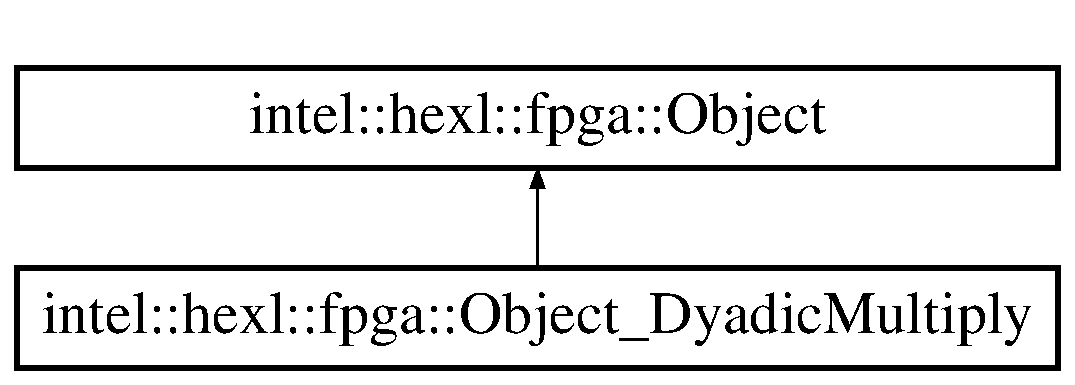
\includegraphics[height=2.000000cm]{structintel_1_1hexl_1_1fpga_1_1Object__DyadicMultiply}
\end{center}
\end{figure}
\subsection*{Public Member Functions}
\begin{DoxyCompactItemize}
\item 
\hyperlink{structintel_1_1hexl_1_1fpga_1_1Object__DyadicMultiply_ae5dfbf4542c84cf45cefbbca727d4409}{Object\-\_\-\-Dyadic\-Multiply} (uint64\-\_\-t $\ast$results, const uint64\-\_\-t $\ast$operand1, const uint64\-\_\-t $\ast$operand2, uint64\-\_\-t n, const uint64\-\_\-t $\ast$moduli, uint64\-\_\-t n\-\_\-moduli)
\end{DoxyCompactItemize}
\subsection*{Public Attributes}
\begin{DoxyCompactItemize}
\item 
uint64\-\_\-t $\ast$ \hyperlink{structintel_1_1hexl_1_1fpga_1_1Object__DyadicMultiply_a89aa54444543557280ff1ebcd250a605}{results\-\_\-}
\item 
const uint64\-\_\-t $\ast$ \hyperlink{structintel_1_1hexl_1_1fpga_1_1Object__DyadicMultiply_af4fecd5061fed1e44ff810d214d9bd73}{operand1\-\_\-}
\item 
const uint64\-\_\-t $\ast$ \hyperlink{structintel_1_1hexl_1_1fpga_1_1Object__DyadicMultiply_a6593688f27a8830c1bb8ce0918db40cd}{operand2\-\_\-}
\item 
uint64\-\_\-t \hyperlink{structintel_1_1hexl_1_1fpga_1_1Object__DyadicMultiply_a836ee7996c0ab56d069fce808e9a58e4}{n\-\_\-}
\item 
const uint64\-\_\-t $\ast$ \hyperlink{structintel_1_1hexl_1_1fpga_1_1Object__DyadicMultiply_a9cf828fe97ff3a03e38597bb9ed8ecf5}{moduli\-\_\-}
\item 
uint64\-\_\-t \hyperlink{structintel_1_1hexl_1_1fpga_1_1Object__DyadicMultiply_ac3d5d1a291f486d9ca341f2f88ed772e}{n\-\_\-moduli\-\_\-}
\end{DoxyCompactItemize}
\subsection*{Additional Inherited Members}


\subsection{Detailed Description}
struct \hyperlink{structintel_1_1hexl_1_1fpga_1_1Object__DyadicMultiply}{Object\-\_\-\-Dyadic\-Multiply} Stores the parameters for the multiplication 


\begin{DoxyParams}[1]{Parameters}
\mbox{\tt out}  & {\em result} & stores the multiplication result \\
\hline
\mbox{\tt in}  & {\em operand1} & stores the first operand for the multiplication \\
\hline
\mbox{\tt in}  & {\em operand2} & stores the second operand for the multiplication \\
\hline
\mbox{\tt in}  & {\em n} & polynomial size \\
\hline
\mbox{\tt in}  & {\em moduli} & vector of moduli \\
\hline
\mbox{\tt in}  & {\em n\-\_\-moduli} & size of the vector of moduli \\
\hline
\end{DoxyParams}


\subsection{Constructor \& Destructor Documentation}
\hypertarget{structintel_1_1hexl_1_1fpga_1_1Object__DyadicMultiply_ae5dfbf4542c84cf45cefbbca727d4409}{\index{intel\-::hexl\-::fpga\-::\-Object\-\_\-\-Dyadic\-Multiply@{intel\-::hexl\-::fpga\-::\-Object\-\_\-\-Dyadic\-Multiply}!Object\-\_\-\-Dyadic\-Multiply@{Object\-\_\-\-Dyadic\-Multiply}}
\index{Object\-\_\-\-Dyadic\-Multiply@{Object\-\_\-\-Dyadic\-Multiply}!intel::hexl::fpga::Object_DyadicMultiply@{intel\-::hexl\-::fpga\-::\-Object\-\_\-\-Dyadic\-Multiply}}
\subsubsection[{Object\-\_\-\-Dyadic\-Multiply}]{\setlength{\rightskip}{0pt plus 5cm}intel\-::hexl\-::fpga\-::\-Object\-\_\-\-Dyadic\-Multiply\-::\-Object\-\_\-\-Dyadic\-Multiply (
\begin{DoxyParamCaption}
\item[{uint64\-\_\-t $\ast$}]{results, }
\item[{const uint64\-\_\-t $\ast$}]{operand1, }
\item[{const uint64\-\_\-t $\ast$}]{operand2, }
\item[{uint64\-\_\-t}]{n, }
\item[{const uint64\-\_\-t $\ast$}]{moduli, }
\item[{uint64\-\_\-t}]{n\-\_\-moduli}
\end{DoxyParamCaption}
)\hspace{0.3cm}{\ttfamily [explicit]}}}\label{structintel_1_1hexl_1_1fpga_1_1Object__DyadicMultiply_ae5dfbf4542c84cf45cefbbca727d4409}


\subsection{Member Data Documentation}
\hypertarget{structintel_1_1hexl_1_1fpga_1_1Object__DyadicMultiply_a9cf828fe97ff3a03e38597bb9ed8ecf5}{\index{intel\-::hexl\-::fpga\-::\-Object\-\_\-\-Dyadic\-Multiply@{intel\-::hexl\-::fpga\-::\-Object\-\_\-\-Dyadic\-Multiply}!moduli\-\_\-@{moduli\-\_\-}}
\index{moduli\-\_\-@{moduli\-\_\-}!intel::hexl::fpga::Object_DyadicMultiply@{intel\-::hexl\-::fpga\-::\-Object\-\_\-\-Dyadic\-Multiply}}
\subsubsection[{moduli\-\_\-}]{\setlength{\rightskip}{0pt plus 5cm}const uint64\-\_\-t$\ast$ intel\-::hexl\-::fpga\-::\-Object\-\_\-\-Dyadic\-Multiply\-::moduli\-\_\-}}\label{structintel_1_1hexl_1_1fpga_1_1Object__DyadicMultiply_a9cf828fe97ff3a03e38597bb9ed8ecf5}
\hypertarget{structintel_1_1hexl_1_1fpga_1_1Object__DyadicMultiply_a836ee7996c0ab56d069fce808e9a58e4}{\index{intel\-::hexl\-::fpga\-::\-Object\-\_\-\-Dyadic\-Multiply@{intel\-::hexl\-::fpga\-::\-Object\-\_\-\-Dyadic\-Multiply}!n\-\_\-@{n\-\_\-}}
\index{n\-\_\-@{n\-\_\-}!intel::hexl::fpga::Object_DyadicMultiply@{intel\-::hexl\-::fpga\-::\-Object\-\_\-\-Dyadic\-Multiply}}
\subsubsection[{n\-\_\-}]{\setlength{\rightskip}{0pt plus 5cm}uint64\-\_\-t intel\-::hexl\-::fpga\-::\-Object\-\_\-\-Dyadic\-Multiply\-::n\-\_\-}}\label{structintel_1_1hexl_1_1fpga_1_1Object__DyadicMultiply_a836ee7996c0ab56d069fce808e9a58e4}
\hypertarget{structintel_1_1hexl_1_1fpga_1_1Object__DyadicMultiply_ac3d5d1a291f486d9ca341f2f88ed772e}{\index{intel\-::hexl\-::fpga\-::\-Object\-\_\-\-Dyadic\-Multiply@{intel\-::hexl\-::fpga\-::\-Object\-\_\-\-Dyadic\-Multiply}!n\-\_\-moduli\-\_\-@{n\-\_\-moduli\-\_\-}}
\index{n\-\_\-moduli\-\_\-@{n\-\_\-moduli\-\_\-}!intel::hexl::fpga::Object_DyadicMultiply@{intel\-::hexl\-::fpga\-::\-Object\-\_\-\-Dyadic\-Multiply}}
\subsubsection[{n\-\_\-moduli\-\_\-}]{\setlength{\rightskip}{0pt plus 5cm}uint64\-\_\-t intel\-::hexl\-::fpga\-::\-Object\-\_\-\-Dyadic\-Multiply\-::n\-\_\-moduli\-\_\-}}\label{structintel_1_1hexl_1_1fpga_1_1Object__DyadicMultiply_ac3d5d1a291f486d9ca341f2f88ed772e}
\hypertarget{structintel_1_1hexl_1_1fpga_1_1Object__DyadicMultiply_af4fecd5061fed1e44ff810d214d9bd73}{\index{intel\-::hexl\-::fpga\-::\-Object\-\_\-\-Dyadic\-Multiply@{intel\-::hexl\-::fpga\-::\-Object\-\_\-\-Dyadic\-Multiply}!operand1\-\_\-@{operand1\-\_\-}}
\index{operand1\-\_\-@{operand1\-\_\-}!intel::hexl::fpga::Object_DyadicMultiply@{intel\-::hexl\-::fpga\-::\-Object\-\_\-\-Dyadic\-Multiply}}
\subsubsection[{operand1\-\_\-}]{\setlength{\rightskip}{0pt plus 5cm}const uint64\-\_\-t$\ast$ intel\-::hexl\-::fpga\-::\-Object\-\_\-\-Dyadic\-Multiply\-::operand1\-\_\-}}\label{structintel_1_1hexl_1_1fpga_1_1Object__DyadicMultiply_af4fecd5061fed1e44ff810d214d9bd73}
\hypertarget{structintel_1_1hexl_1_1fpga_1_1Object__DyadicMultiply_a6593688f27a8830c1bb8ce0918db40cd}{\index{intel\-::hexl\-::fpga\-::\-Object\-\_\-\-Dyadic\-Multiply@{intel\-::hexl\-::fpga\-::\-Object\-\_\-\-Dyadic\-Multiply}!operand2\-\_\-@{operand2\-\_\-}}
\index{operand2\-\_\-@{operand2\-\_\-}!intel::hexl::fpga::Object_DyadicMultiply@{intel\-::hexl\-::fpga\-::\-Object\-\_\-\-Dyadic\-Multiply}}
\subsubsection[{operand2\-\_\-}]{\setlength{\rightskip}{0pt plus 5cm}const uint64\-\_\-t$\ast$ intel\-::hexl\-::fpga\-::\-Object\-\_\-\-Dyadic\-Multiply\-::operand2\-\_\-}}\label{structintel_1_1hexl_1_1fpga_1_1Object__DyadicMultiply_a6593688f27a8830c1bb8ce0918db40cd}
\hypertarget{structintel_1_1hexl_1_1fpga_1_1Object__DyadicMultiply_a89aa54444543557280ff1ebcd250a605}{\index{intel\-::hexl\-::fpga\-::\-Object\-\_\-\-Dyadic\-Multiply@{intel\-::hexl\-::fpga\-::\-Object\-\_\-\-Dyadic\-Multiply}!results\-\_\-@{results\-\_\-}}
\index{results\-\_\-@{results\-\_\-}!intel::hexl::fpga::Object_DyadicMultiply@{intel\-::hexl\-::fpga\-::\-Object\-\_\-\-Dyadic\-Multiply}}
\subsubsection[{results\-\_\-}]{\setlength{\rightskip}{0pt plus 5cm}uint64\-\_\-t$\ast$ intel\-::hexl\-::fpga\-::\-Object\-\_\-\-Dyadic\-Multiply\-::results\-\_\-}}\label{structintel_1_1hexl_1_1fpga_1_1Object__DyadicMultiply_a89aa54444543557280ff1ebcd250a605}


The documentation for this struct was generated from the following file\-:\begin{DoxyCompactItemize}
\item 
\hyperlink{fpga_8h}{fpga.\-h}\end{DoxyCompactItemize}

\hypertarget{structintel_1_1hexl_1_1fpga_1_1Object__INTT}{\section{intel\-:\-:hexl\-:\-:fpga\-:\-:Object\-\_\-\-I\-N\-T\-T Struct Reference}
\label{structintel_1_1hexl_1_1fpga_1_1Object__INTT}\index{intel\-::hexl\-::fpga\-::\-Object\-\_\-\-I\-N\-T\-T@{intel\-::hexl\-::fpga\-::\-Object\-\_\-\-I\-N\-T\-T}}
}


Struct \hyperlink{structintel_1_1hexl_1_1fpga_1_1Object}{Object} I\-N\-T\-T Stores the Inverse Number Theoretic Transform parameters.  




{\ttfamily \#include $<$fpga.\-h$>$}

Inheritance diagram for intel\-:\-:hexl\-:\-:fpga\-:\-:Object\-\_\-\-I\-N\-T\-T\-:\begin{figure}[H]
\begin{center}
\leavevmode
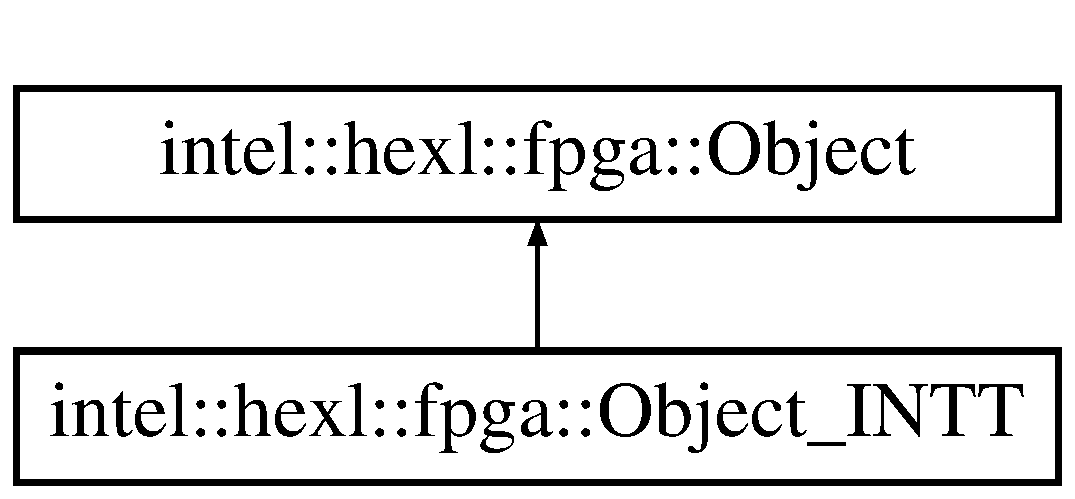
\includegraphics[height=2.000000cm]{structintel_1_1hexl_1_1fpga_1_1Object__INTT}
\end{center}
\end{figure}
\subsection*{Public Member Functions}
\begin{DoxyCompactItemize}
\item 
\hyperlink{structintel_1_1hexl_1_1fpga_1_1Object__INTT_ae22d0f99e890bde6201cbcb3eb4f0cd9}{Object\-\_\-\-I\-N\-T\-T} (uint64\-\_\-t $\ast$coeff\-\_\-poly, const uint64\-\_\-t $\ast$inv\-\_\-root\-\_\-of\-\_\-unity\-\_\-powers, const uint64\-\_\-t $\ast$precon\-\_\-inv\-\_\-root\-\_\-of\-\_\-unity\-\_\-powers, uint64\-\_\-t coeff\-\_\-modulus, uint64\-\_\-t inv\-\_\-n, uint64\-\_\-t inv\-\_\-n\-\_\-w, uint64\-\_\-t n, bool fence=false)
\end{DoxyCompactItemize}
\subsection*{Public Attributes}
\begin{DoxyCompactItemize}
\item 
uint64\-\_\-t $\ast$ \hyperlink{structintel_1_1hexl_1_1fpga_1_1Object__INTT_a4193d2648e27da868ba8790083a6b749}{coeff\-\_\-poly\-\_\-}
\item 
const uint64\-\_\-t $\ast$ \hyperlink{structintel_1_1hexl_1_1fpga_1_1Object__INTT_a4821a007e352a4f2f5eff215476f2d5f}{inv\-\_\-root\-\_\-of\-\_\-unity\-\_\-powers\-\_\-}
\item 
const uint64\-\_\-t $\ast$ \hyperlink{structintel_1_1hexl_1_1fpga_1_1Object__INTT_a916b6af204fa6a6236b3d7a332bb9999}{precon\-\_\-inv\-\_\-root\-\_\-of\-\_\-unity\-\_\-powers\-\_\-}
\item 
uint64\-\_\-t \hyperlink{structintel_1_1hexl_1_1fpga_1_1Object__INTT_a32f41552e25ee8102e9844040a3dbce5}{coeff\-\_\-modulus\-\_\-}
\item 
uint64\-\_\-t \hyperlink{structintel_1_1hexl_1_1fpga_1_1Object__INTT_a3b21373f1684a50b92b48938b3705fd8}{inv\-\_\-n\-\_\-}
\item 
uint64\-\_\-t \hyperlink{structintel_1_1hexl_1_1fpga_1_1Object__INTT_a09781e11982cbac5a01a16610f725f79}{inv\-\_\-n\-\_\-w\-\_\-}
\item 
uint64\-\_\-t \hyperlink{structintel_1_1hexl_1_1fpga_1_1Object__INTT_a3e0c80ff67c84bbae44082bca8a6a1f5}{n\-\_\-}
\end{DoxyCompactItemize}
\subsection*{Additional Inherited Members}


\subsection{Detailed Description}
Struct \hyperlink{structintel_1_1hexl_1_1fpga_1_1Object}{Object} I\-N\-T\-T Stores the Inverse Number Theoretic Transform parameters. 


\begin{DoxyParams}[1]{Parameters}
\mbox{\tt in}  & {\em coeff\-\_\-poly} & polynomial coefficients \\
\hline
\mbox{\tt out}  & {\em coeff\-\_\-poly} & polynomial coefficients \\
\hline
\mbox{\tt in}  & {\em inv\-\_\-root\-\_\-of\-\_\-unity\-\_\-powers} & twiddle factors for the inverse transform \\
\hline
\mbox{\tt in}  & {\em precon\-\_\-inv\-\_\-root\-\_\-of\-\_\-unity\-\_\-powers} & inverse twiddle factors for the inverse transform \\
\hline
\mbox{\tt in}  & {\em coeff\-\_\-modulus} & polynomial coefficients modulus \\
\hline
\mbox{\tt in}  & {\em inv\-\_\-n} & normalization factor for the coefficients \\
\hline
\mbox{\tt in}  & {\em inv\-\_\-n\-\_\-w} & normalization factor for the constant factor \\
\hline
\mbox{\tt in}  & {\em n} & polynomial size \\
\hline
\end{DoxyParams}


\subsection{Constructor \& Destructor Documentation}
\hypertarget{structintel_1_1hexl_1_1fpga_1_1Object__INTT_ae22d0f99e890bde6201cbcb3eb4f0cd9}{\index{intel\-::hexl\-::fpga\-::\-Object\-\_\-\-I\-N\-T\-T@{intel\-::hexl\-::fpga\-::\-Object\-\_\-\-I\-N\-T\-T}!Object\-\_\-\-I\-N\-T\-T@{Object\-\_\-\-I\-N\-T\-T}}
\index{Object\-\_\-\-I\-N\-T\-T@{Object\-\_\-\-I\-N\-T\-T}!intel::hexl::fpga::Object_INTT@{intel\-::hexl\-::fpga\-::\-Object\-\_\-\-I\-N\-T\-T}}
\subsubsection[{Object\-\_\-\-I\-N\-T\-T}]{\setlength{\rightskip}{0pt plus 5cm}intel\-::hexl\-::fpga\-::\-Object\-\_\-\-I\-N\-T\-T\-::\-Object\-\_\-\-I\-N\-T\-T (
\begin{DoxyParamCaption}
\item[{uint64\-\_\-t $\ast$}]{coeff\-\_\-poly, }
\item[{const uint64\-\_\-t $\ast$}]{inv\-\_\-root\-\_\-of\-\_\-unity\-\_\-powers, }
\item[{const uint64\-\_\-t $\ast$}]{precon\-\_\-inv\-\_\-root\-\_\-of\-\_\-unity\-\_\-powers, }
\item[{uint64\-\_\-t}]{coeff\-\_\-modulus, }
\item[{uint64\-\_\-t}]{inv\-\_\-n, }
\item[{uint64\-\_\-t}]{inv\-\_\-n\-\_\-w, }
\item[{uint64\-\_\-t}]{n, }
\item[{bool}]{fence = {\ttfamily false}}
\end{DoxyParamCaption}
)\hspace{0.3cm}{\ttfamily [explicit]}}}\label{structintel_1_1hexl_1_1fpga_1_1Object__INTT_ae22d0f99e890bde6201cbcb3eb4f0cd9}


\subsection{Member Data Documentation}
\hypertarget{structintel_1_1hexl_1_1fpga_1_1Object__INTT_a32f41552e25ee8102e9844040a3dbce5}{\index{intel\-::hexl\-::fpga\-::\-Object\-\_\-\-I\-N\-T\-T@{intel\-::hexl\-::fpga\-::\-Object\-\_\-\-I\-N\-T\-T}!coeff\-\_\-modulus\-\_\-@{coeff\-\_\-modulus\-\_\-}}
\index{coeff\-\_\-modulus\-\_\-@{coeff\-\_\-modulus\-\_\-}!intel::hexl::fpga::Object_INTT@{intel\-::hexl\-::fpga\-::\-Object\-\_\-\-I\-N\-T\-T}}
\subsubsection[{coeff\-\_\-modulus\-\_\-}]{\setlength{\rightskip}{0pt plus 5cm}uint64\-\_\-t intel\-::hexl\-::fpga\-::\-Object\-\_\-\-I\-N\-T\-T\-::coeff\-\_\-modulus\-\_\-}}\label{structintel_1_1hexl_1_1fpga_1_1Object__INTT_a32f41552e25ee8102e9844040a3dbce5}
\hypertarget{structintel_1_1hexl_1_1fpga_1_1Object__INTT_a4193d2648e27da868ba8790083a6b749}{\index{intel\-::hexl\-::fpga\-::\-Object\-\_\-\-I\-N\-T\-T@{intel\-::hexl\-::fpga\-::\-Object\-\_\-\-I\-N\-T\-T}!coeff\-\_\-poly\-\_\-@{coeff\-\_\-poly\-\_\-}}
\index{coeff\-\_\-poly\-\_\-@{coeff\-\_\-poly\-\_\-}!intel::hexl::fpga::Object_INTT@{intel\-::hexl\-::fpga\-::\-Object\-\_\-\-I\-N\-T\-T}}
\subsubsection[{coeff\-\_\-poly\-\_\-}]{\setlength{\rightskip}{0pt plus 5cm}uint64\-\_\-t$\ast$ intel\-::hexl\-::fpga\-::\-Object\-\_\-\-I\-N\-T\-T\-::coeff\-\_\-poly\-\_\-}}\label{structintel_1_1hexl_1_1fpga_1_1Object__INTT_a4193d2648e27da868ba8790083a6b749}
\hypertarget{structintel_1_1hexl_1_1fpga_1_1Object__INTT_a3b21373f1684a50b92b48938b3705fd8}{\index{intel\-::hexl\-::fpga\-::\-Object\-\_\-\-I\-N\-T\-T@{intel\-::hexl\-::fpga\-::\-Object\-\_\-\-I\-N\-T\-T}!inv\-\_\-n\-\_\-@{inv\-\_\-n\-\_\-}}
\index{inv\-\_\-n\-\_\-@{inv\-\_\-n\-\_\-}!intel::hexl::fpga::Object_INTT@{intel\-::hexl\-::fpga\-::\-Object\-\_\-\-I\-N\-T\-T}}
\subsubsection[{inv\-\_\-n\-\_\-}]{\setlength{\rightskip}{0pt plus 5cm}uint64\-\_\-t intel\-::hexl\-::fpga\-::\-Object\-\_\-\-I\-N\-T\-T\-::inv\-\_\-n\-\_\-}}\label{structintel_1_1hexl_1_1fpga_1_1Object__INTT_a3b21373f1684a50b92b48938b3705fd8}
\hypertarget{structintel_1_1hexl_1_1fpga_1_1Object__INTT_a09781e11982cbac5a01a16610f725f79}{\index{intel\-::hexl\-::fpga\-::\-Object\-\_\-\-I\-N\-T\-T@{intel\-::hexl\-::fpga\-::\-Object\-\_\-\-I\-N\-T\-T}!inv\-\_\-n\-\_\-w\-\_\-@{inv\-\_\-n\-\_\-w\-\_\-}}
\index{inv\-\_\-n\-\_\-w\-\_\-@{inv\-\_\-n\-\_\-w\-\_\-}!intel::hexl::fpga::Object_INTT@{intel\-::hexl\-::fpga\-::\-Object\-\_\-\-I\-N\-T\-T}}
\subsubsection[{inv\-\_\-n\-\_\-w\-\_\-}]{\setlength{\rightskip}{0pt plus 5cm}uint64\-\_\-t intel\-::hexl\-::fpga\-::\-Object\-\_\-\-I\-N\-T\-T\-::inv\-\_\-n\-\_\-w\-\_\-}}\label{structintel_1_1hexl_1_1fpga_1_1Object__INTT_a09781e11982cbac5a01a16610f725f79}
\hypertarget{structintel_1_1hexl_1_1fpga_1_1Object__INTT_a4821a007e352a4f2f5eff215476f2d5f}{\index{intel\-::hexl\-::fpga\-::\-Object\-\_\-\-I\-N\-T\-T@{intel\-::hexl\-::fpga\-::\-Object\-\_\-\-I\-N\-T\-T}!inv\-\_\-root\-\_\-of\-\_\-unity\-\_\-powers\-\_\-@{inv\-\_\-root\-\_\-of\-\_\-unity\-\_\-powers\-\_\-}}
\index{inv\-\_\-root\-\_\-of\-\_\-unity\-\_\-powers\-\_\-@{inv\-\_\-root\-\_\-of\-\_\-unity\-\_\-powers\-\_\-}!intel::hexl::fpga::Object_INTT@{intel\-::hexl\-::fpga\-::\-Object\-\_\-\-I\-N\-T\-T}}
\subsubsection[{inv\-\_\-root\-\_\-of\-\_\-unity\-\_\-powers\-\_\-}]{\setlength{\rightskip}{0pt plus 5cm}const uint64\-\_\-t$\ast$ intel\-::hexl\-::fpga\-::\-Object\-\_\-\-I\-N\-T\-T\-::inv\-\_\-root\-\_\-of\-\_\-unity\-\_\-powers\-\_\-}}\label{structintel_1_1hexl_1_1fpga_1_1Object__INTT_a4821a007e352a4f2f5eff215476f2d5f}
\hypertarget{structintel_1_1hexl_1_1fpga_1_1Object__INTT_a3e0c80ff67c84bbae44082bca8a6a1f5}{\index{intel\-::hexl\-::fpga\-::\-Object\-\_\-\-I\-N\-T\-T@{intel\-::hexl\-::fpga\-::\-Object\-\_\-\-I\-N\-T\-T}!n\-\_\-@{n\-\_\-}}
\index{n\-\_\-@{n\-\_\-}!intel::hexl::fpga::Object_INTT@{intel\-::hexl\-::fpga\-::\-Object\-\_\-\-I\-N\-T\-T}}
\subsubsection[{n\-\_\-}]{\setlength{\rightskip}{0pt plus 5cm}uint64\-\_\-t intel\-::hexl\-::fpga\-::\-Object\-\_\-\-I\-N\-T\-T\-::n\-\_\-}}\label{structintel_1_1hexl_1_1fpga_1_1Object__INTT_a3e0c80ff67c84bbae44082bca8a6a1f5}
\hypertarget{structintel_1_1hexl_1_1fpga_1_1Object__INTT_a916b6af204fa6a6236b3d7a332bb9999}{\index{intel\-::hexl\-::fpga\-::\-Object\-\_\-\-I\-N\-T\-T@{intel\-::hexl\-::fpga\-::\-Object\-\_\-\-I\-N\-T\-T}!precon\-\_\-inv\-\_\-root\-\_\-of\-\_\-unity\-\_\-powers\-\_\-@{precon\-\_\-inv\-\_\-root\-\_\-of\-\_\-unity\-\_\-powers\-\_\-}}
\index{precon\-\_\-inv\-\_\-root\-\_\-of\-\_\-unity\-\_\-powers\-\_\-@{precon\-\_\-inv\-\_\-root\-\_\-of\-\_\-unity\-\_\-powers\-\_\-}!intel::hexl::fpga::Object_INTT@{intel\-::hexl\-::fpga\-::\-Object\-\_\-\-I\-N\-T\-T}}
\subsubsection[{precon\-\_\-inv\-\_\-root\-\_\-of\-\_\-unity\-\_\-powers\-\_\-}]{\setlength{\rightskip}{0pt plus 5cm}const uint64\-\_\-t$\ast$ intel\-::hexl\-::fpga\-::\-Object\-\_\-\-I\-N\-T\-T\-::precon\-\_\-inv\-\_\-root\-\_\-of\-\_\-unity\-\_\-powers\-\_\-}}\label{structintel_1_1hexl_1_1fpga_1_1Object__INTT_a916b6af204fa6a6236b3d7a332bb9999}


The documentation for this struct was generated from the following file\-:\begin{DoxyCompactItemize}
\item 
\hyperlink{fpga_8h}{fpga.\-h}\end{DoxyCompactItemize}

\hypertarget{structintel_1_1hexl_1_1fpga_1_1Object__NTT}{\section{intel\-:\-:hexl\-:\-:fpga\-:\-:Object\-\_\-\-N\-T\-T Struct Reference}
\label{structintel_1_1hexl_1_1fpga_1_1Object__NTT}\index{intel\-::hexl\-::fpga\-::\-Object\-\_\-\-N\-T\-T@{intel\-::hexl\-::fpga\-::\-Object\-\_\-\-N\-T\-T}}
}


Struct \hyperlink{structintel_1_1hexl_1_1fpga_1_1Object}{Object} N\-T\-T Stores the Number Theoretic Transform parameters.  




{\ttfamily \#include $<$fpga.\-h$>$}

Inheritance diagram for intel\-:\-:hexl\-:\-:fpga\-:\-:Object\-\_\-\-N\-T\-T\-:\begin{figure}[H]
\begin{center}
\leavevmode
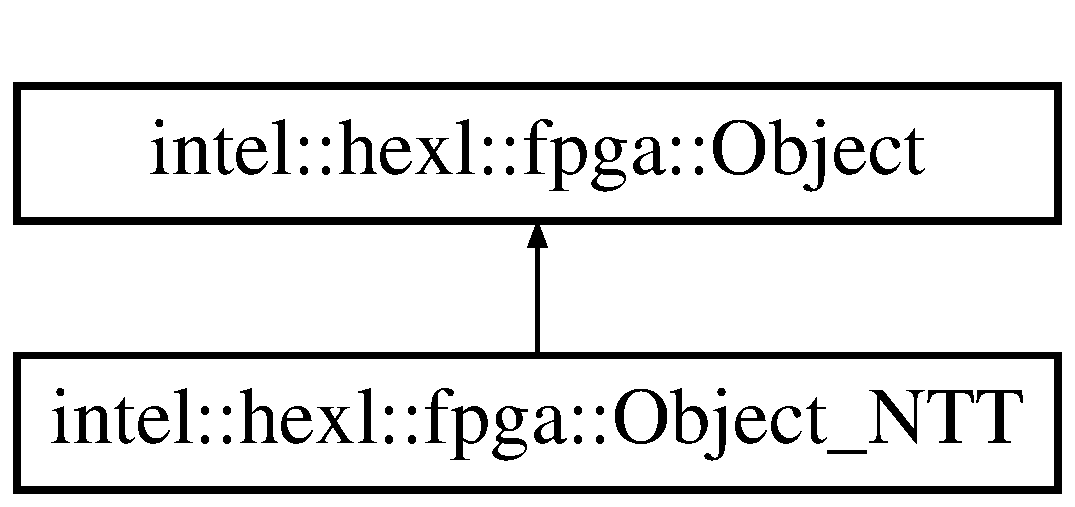
\includegraphics[height=2.000000cm]{structintel_1_1hexl_1_1fpga_1_1Object__NTT}
\end{center}
\end{figure}
\subsection*{Public Member Functions}
\begin{DoxyCompactItemize}
\item 
\hyperlink{structintel_1_1hexl_1_1fpga_1_1Object__NTT_a0e477200da8200247454023763e37cf4}{Object\-\_\-\-N\-T\-T} (uint64\-\_\-t $\ast$coeff\-\_\-poly, const uint64\-\_\-t $\ast$root\-\_\-of\-\_\-unity\-\_\-powers, const uint64\-\_\-t $\ast$precon\-\_\-root\-\_\-of\-\_\-unity\-\_\-powers, uint64\-\_\-t coeff\-\_\-modulus, uint64\-\_\-t n)
\end{DoxyCompactItemize}
\subsection*{Public Attributes}
\begin{DoxyCompactItemize}
\item 
uint64\-\_\-t $\ast$ \hyperlink{structintel_1_1hexl_1_1fpga_1_1Object__NTT_a456d2d8f4eac2f2f5360ce83b4bed98d}{coeff\-\_\-poly\-\_\-}
\item 
const uint64\-\_\-t $\ast$ \hyperlink{structintel_1_1hexl_1_1fpga_1_1Object__NTT_a02ad1422d0256bfe1cee773d45faca5f}{root\-\_\-of\-\_\-unity\-\_\-powers\-\_\-}
\item 
const uint64\-\_\-t $\ast$ \hyperlink{structintel_1_1hexl_1_1fpga_1_1Object__NTT_ac7d181c6f3d75a62f42e3115541450a2}{precon\-\_\-root\-\_\-of\-\_\-unity\-\_\-powers\-\_\-}
\item 
uint64\-\_\-t \hyperlink{structintel_1_1hexl_1_1fpga_1_1Object__NTT_a534bfc6c711a0dd767d511087a86666d}{coeff\-\_\-modulus\-\_\-}
\item 
uint64\-\_\-t \hyperlink{structintel_1_1hexl_1_1fpga_1_1Object__NTT_a680eca9bf78e81f26426cf0dc9b52f5e}{n\-\_\-}
\end{DoxyCompactItemize}
\subsection*{Additional Inherited Members}


\subsection{Detailed Description}
Struct \hyperlink{structintel_1_1hexl_1_1fpga_1_1Object}{Object} N\-T\-T Stores the Number Theoretic Transform parameters. 


\begin{DoxyParams}[1]{Parameters}
\mbox{\tt in}  & {\em coeff\-\_\-poly} & polynomial coefficients \\
\hline
\mbox{\tt out}  & {\em coeff\-\_\-poly} & polynomial coefficients \\
\hline
\mbox{\tt in}  & {\em root\-\_\-of\-\_\-unity\-\_\-powers} & twiddle factors \\
\hline
\mbox{\tt in}  & {\em precon\-\_\-root\-\_\-of\-\_\-unity\-\_\-powers} & inverse twiddle factors \\
\hline
\mbox{\tt in}  & {\em coeff\-\_\-modulus} & polynomial coefficients modulus \\
\hline
\mbox{\tt in}  & {\em n} & polynomial size in powers of two \\
\hline
\end{DoxyParams}


\subsection{Constructor \& Destructor Documentation}
\hypertarget{structintel_1_1hexl_1_1fpga_1_1Object__NTT_a0e477200da8200247454023763e37cf4}{\index{intel\-::hexl\-::fpga\-::\-Object\-\_\-\-N\-T\-T@{intel\-::hexl\-::fpga\-::\-Object\-\_\-\-N\-T\-T}!Object\-\_\-\-N\-T\-T@{Object\-\_\-\-N\-T\-T}}
\index{Object\-\_\-\-N\-T\-T@{Object\-\_\-\-N\-T\-T}!intel::hexl::fpga::Object_NTT@{intel\-::hexl\-::fpga\-::\-Object\-\_\-\-N\-T\-T}}
\subsubsection[{Object\-\_\-\-N\-T\-T}]{\setlength{\rightskip}{0pt plus 5cm}intel\-::hexl\-::fpga\-::\-Object\-\_\-\-N\-T\-T\-::\-Object\-\_\-\-N\-T\-T (
\begin{DoxyParamCaption}
\item[{uint64\-\_\-t $\ast$}]{coeff\-\_\-poly, }
\item[{const uint64\-\_\-t $\ast$}]{root\-\_\-of\-\_\-unity\-\_\-powers, }
\item[{const uint64\-\_\-t $\ast$}]{precon\-\_\-root\-\_\-of\-\_\-unity\-\_\-powers, }
\item[{uint64\-\_\-t}]{coeff\-\_\-modulus, }
\item[{uint64\-\_\-t}]{n}
\end{DoxyParamCaption}
)\hspace{0.3cm}{\ttfamily [explicit]}}}\label{structintel_1_1hexl_1_1fpga_1_1Object__NTT_a0e477200da8200247454023763e37cf4}


\subsection{Member Data Documentation}
\hypertarget{structintel_1_1hexl_1_1fpga_1_1Object__NTT_a534bfc6c711a0dd767d511087a86666d}{\index{intel\-::hexl\-::fpga\-::\-Object\-\_\-\-N\-T\-T@{intel\-::hexl\-::fpga\-::\-Object\-\_\-\-N\-T\-T}!coeff\-\_\-modulus\-\_\-@{coeff\-\_\-modulus\-\_\-}}
\index{coeff\-\_\-modulus\-\_\-@{coeff\-\_\-modulus\-\_\-}!intel::hexl::fpga::Object_NTT@{intel\-::hexl\-::fpga\-::\-Object\-\_\-\-N\-T\-T}}
\subsubsection[{coeff\-\_\-modulus\-\_\-}]{\setlength{\rightskip}{0pt plus 5cm}uint64\-\_\-t intel\-::hexl\-::fpga\-::\-Object\-\_\-\-N\-T\-T\-::coeff\-\_\-modulus\-\_\-}}\label{structintel_1_1hexl_1_1fpga_1_1Object__NTT_a534bfc6c711a0dd767d511087a86666d}
\hypertarget{structintel_1_1hexl_1_1fpga_1_1Object__NTT_a456d2d8f4eac2f2f5360ce83b4bed98d}{\index{intel\-::hexl\-::fpga\-::\-Object\-\_\-\-N\-T\-T@{intel\-::hexl\-::fpga\-::\-Object\-\_\-\-N\-T\-T}!coeff\-\_\-poly\-\_\-@{coeff\-\_\-poly\-\_\-}}
\index{coeff\-\_\-poly\-\_\-@{coeff\-\_\-poly\-\_\-}!intel::hexl::fpga::Object_NTT@{intel\-::hexl\-::fpga\-::\-Object\-\_\-\-N\-T\-T}}
\subsubsection[{coeff\-\_\-poly\-\_\-}]{\setlength{\rightskip}{0pt plus 5cm}uint64\-\_\-t$\ast$ intel\-::hexl\-::fpga\-::\-Object\-\_\-\-N\-T\-T\-::coeff\-\_\-poly\-\_\-}}\label{structintel_1_1hexl_1_1fpga_1_1Object__NTT_a456d2d8f4eac2f2f5360ce83b4bed98d}
\hypertarget{structintel_1_1hexl_1_1fpga_1_1Object__NTT_a680eca9bf78e81f26426cf0dc9b52f5e}{\index{intel\-::hexl\-::fpga\-::\-Object\-\_\-\-N\-T\-T@{intel\-::hexl\-::fpga\-::\-Object\-\_\-\-N\-T\-T}!n\-\_\-@{n\-\_\-}}
\index{n\-\_\-@{n\-\_\-}!intel::hexl::fpga::Object_NTT@{intel\-::hexl\-::fpga\-::\-Object\-\_\-\-N\-T\-T}}
\subsubsection[{n\-\_\-}]{\setlength{\rightskip}{0pt plus 5cm}uint64\-\_\-t intel\-::hexl\-::fpga\-::\-Object\-\_\-\-N\-T\-T\-::n\-\_\-}}\label{structintel_1_1hexl_1_1fpga_1_1Object__NTT_a680eca9bf78e81f26426cf0dc9b52f5e}
\hypertarget{structintel_1_1hexl_1_1fpga_1_1Object__NTT_ac7d181c6f3d75a62f42e3115541450a2}{\index{intel\-::hexl\-::fpga\-::\-Object\-\_\-\-N\-T\-T@{intel\-::hexl\-::fpga\-::\-Object\-\_\-\-N\-T\-T}!precon\-\_\-root\-\_\-of\-\_\-unity\-\_\-powers\-\_\-@{precon\-\_\-root\-\_\-of\-\_\-unity\-\_\-powers\-\_\-}}
\index{precon\-\_\-root\-\_\-of\-\_\-unity\-\_\-powers\-\_\-@{precon\-\_\-root\-\_\-of\-\_\-unity\-\_\-powers\-\_\-}!intel::hexl::fpga::Object_NTT@{intel\-::hexl\-::fpga\-::\-Object\-\_\-\-N\-T\-T}}
\subsubsection[{precon\-\_\-root\-\_\-of\-\_\-unity\-\_\-powers\-\_\-}]{\setlength{\rightskip}{0pt plus 5cm}const uint64\-\_\-t$\ast$ intel\-::hexl\-::fpga\-::\-Object\-\_\-\-N\-T\-T\-::precon\-\_\-root\-\_\-of\-\_\-unity\-\_\-powers\-\_\-}}\label{structintel_1_1hexl_1_1fpga_1_1Object__NTT_ac7d181c6f3d75a62f42e3115541450a2}
\hypertarget{structintel_1_1hexl_1_1fpga_1_1Object__NTT_a02ad1422d0256bfe1cee773d45faca5f}{\index{intel\-::hexl\-::fpga\-::\-Object\-\_\-\-N\-T\-T@{intel\-::hexl\-::fpga\-::\-Object\-\_\-\-N\-T\-T}!root\-\_\-of\-\_\-unity\-\_\-powers\-\_\-@{root\-\_\-of\-\_\-unity\-\_\-powers\-\_\-}}
\index{root\-\_\-of\-\_\-unity\-\_\-powers\-\_\-@{root\-\_\-of\-\_\-unity\-\_\-powers\-\_\-}!intel::hexl::fpga::Object_NTT@{intel\-::hexl\-::fpga\-::\-Object\-\_\-\-N\-T\-T}}
\subsubsection[{root\-\_\-of\-\_\-unity\-\_\-powers\-\_\-}]{\setlength{\rightskip}{0pt plus 5cm}const uint64\-\_\-t$\ast$ intel\-::hexl\-::fpga\-::\-Object\-\_\-\-N\-T\-T\-::root\-\_\-of\-\_\-unity\-\_\-powers\-\_\-}}\label{structintel_1_1hexl_1_1fpga_1_1Object__NTT_a02ad1422d0256bfe1cee773d45faca5f}


The documentation for this struct was generated from the following file\-:\begin{DoxyCompactItemize}
\item 
\hyperlink{fpga_8h}{fpga.\-h}\end{DoxyCompactItemize}

\hypertarget{structhetest_1_1utils_1_1AlignedAllocator_1_1rebind}{\section{hetest\-:\-:utils\-:\-:Aligned\-Allocator$<$ T, Alignment $>$\-:\-:rebind$<$ U $>$ Struct Template Reference}
\label{structhetest_1_1utils_1_1AlignedAllocator_1_1rebind}\index{hetest\-::utils\-::\-Aligned\-Allocator$<$ T, Alignment $>$\-::rebind$<$ U $>$@{hetest\-::utils\-::\-Aligned\-Allocator$<$ T, Alignment $>$\-::rebind$<$ U $>$}}
}


{\ttfamily \#include $<$utils-\/test.\-hpp$>$}

\subsection*{Public Types}
\begin{DoxyCompactItemize}
\item 
using \hyperlink{structhetest_1_1utils_1_1AlignedAllocator_1_1rebind_ac55bc630e5d5c06ccfb3cdfe249f0a47}{other} = \hyperlink{classhetest_1_1utils_1_1AlignedAllocator}{Aligned\-Allocator}$<$ U, Alignment $>$
\end{DoxyCompactItemize}


\subsection{Member Typedef Documentation}
\hypertarget{structhetest_1_1utils_1_1AlignedAllocator_1_1rebind_ac55bc630e5d5c06ccfb3cdfe249f0a47}{\index{hetest\-::utils\-::\-Aligned\-Allocator\-::rebind@{hetest\-::utils\-::\-Aligned\-Allocator\-::rebind}!other@{other}}
\index{other@{other}!hetest::utils::AlignedAllocator::rebind@{hetest\-::utils\-::\-Aligned\-Allocator\-::rebind}}
\subsubsection[{other}]{\setlength{\rightskip}{0pt plus 5cm}template$<$typename T, uint64\-\_\-t Alignment$>$ template$<$typename U $>$ using {\bf hetest\-::utils\-::\-Aligned\-Allocator}$<$ T, Alignment $>$\-::{\bf rebind}$<$ U $>$\-::{\bf other} =  {\bf Aligned\-Allocator}$<$U, Alignment$>$}}\label{structhetest_1_1utils_1_1AlignedAllocator_1_1rebind_ac55bc630e5d5c06ccfb3cdfe249f0a47}


The documentation for this struct was generated from the following file\-:\begin{DoxyCompactItemize}
\item 
\hyperlink{utils-test_8hpp}{utils-\/test.\-hpp}\end{DoxyCompactItemize}

\hypertarget{classintel_1_1hexl_1_1fpga_1_1StackTrace}{\section{intel\-:\-:hexl\-:\-:fpga\-:\-:Stack\-Trace Class Reference}
\label{classintel_1_1hexl_1_1fpga_1_1StackTrace}\index{intel\-::hexl\-::fpga\-::\-Stack\-Trace@{intel\-::hexl\-::fpga\-::\-Stack\-Trace}}
}


Class \hyperlink{classintel_1_1hexl_1_1fpga_1_1StackTrace}{Stack\-Trace} Allows the investigation of the traces  dump Dumps the traces.  




{\ttfamily \#include $<$stack\-\_\-trace.\-h$>$}

\subsection*{Public Member Functions}
\begin{DoxyCompactItemize}
\item 
virtual \hyperlink{classintel_1_1hexl_1_1fpga_1_1StackTrace_ae3665f0cc2097380b9a5fdd6330df6e5}{$\sim$\-Stack\-Trace} ()=default
\item 
virtual void \hyperlink{classintel_1_1hexl_1_1fpga_1_1StackTrace_a333d1509937db15dae0780b20da5b0ea}{dump} (std\-::ostream \&os)=0
\end{DoxyCompactItemize}
\subsection*{Static Public Member Functions}
\begin{DoxyCompactItemize}
\item 
static \hyperlink{classintel_1_1hexl_1_1fpga_1_1StackTrace}{Stack\-Trace} $\ast$ \hyperlink{classintel_1_1hexl_1_1fpga_1_1StackTrace_a13e71720d91b3ad78008fc4b71fe159c}{stack} ()
\end{DoxyCompactItemize}
\subsection*{Protected Member Functions}
\begin{DoxyCompactItemize}
\item 
\hyperlink{classintel_1_1hexl_1_1fpga_1_1StackTrace_a33b7e4305ba5ebd6d3210971528770f5}{Stack\-Trace} ()
\end{DoxyCompactItemize}


\subsection{Detailed Description}
Class \hyperlink{classintel_1_1hexl_1_1fpga_1_1StackTrace}{Stack\-Trace} Allows the investigation of the traces  dump Dumps the traces. 


\begin{DoxyParams}[1]{Parameters}
\mbox{\tt in}  & {\em os} & vector of traces \\
\hline
\end{DoxyParams}


\subsection{Constructor \& Destructor Documentation}
\hypertarget{classintel_1_1hexl_1_1fpga_1_1StackTrace_ae3665f0cc2097380b9a5fdd6330df6e5}{\index{intel\-::hexl\-::fpga\-::\-Stack\-Trace@{intel\-::hexl\-::fpga\-::\-Stack\-Trace}!$\sim$\-Stack\-Trace@{$\sim$\-Stack\-Trace}}
\index{$\sim$\-Stack\-Trace@{$\sim$\-Stack\-Trace}!intel::hexl::fpga::StackTrace@{intel\-::hexl\-::fpga\-::\-Stack\-Trace}}
\subsubsection[{$\sim$\-Stack\-Trace}]{\setlength{\rightskip}{0pt plus 5cm}virtual intel\-::hexl\-::fpga\-::\-Stack\-Trace\-::$\sim$\-Stack\-Trace (
\begin{DoxyParamCaption}
{}
\end{DoxyParamCaption}
)\hspace{0.3cm}{\ttfamily [virtual]}, {\ttfamily [default]}}}\label{classintel_1_1hexl_1_1fpga_1_1StackTrace_ae3665f0cc2097380b9a5fdd6330df6e5}
\hypertarget{classintel_1_1hexl_1_1fpga_1_1StackTrace_a33b7e4305ba5ebd6d3210971528770f5}{\index{intel\-::hexl\-::fpga\-::\-Stack\-Trace@{intel\-::hexl\-::fpga\-::\-Stack\-Trace}!Stack\-Trace@{Stack\-Trace}}
\index{Stack\-Trace@{Stack\-Trace}!intel::hexl::fpga::StackTrace@{intel\-::hexl\-::fpga\-::\-Stack\-Trace}}
\subsubsection[{Stack\-Trace}]{\setlength{\rightskip}{0pt plus 5cm}intel\-::hexl\-::fpga\-::\-Stack\-Trace\-::\-Stack\-Trace (
\begin{DoxyParamCaption}
{}
\end{DoxyParamCaption}
)\hspace{0.3cm}{\ttfamily [inline]}, {\ttfamily [protected]}}}\label{classintel_1_1hexl_1_1fpga_1_1StackTrace_a33b7e4305ba5ebd6d3210971528770f5}


\subsection{Member Function Documentation}
\hypertarget{classintel_1_1hexl_1_1fpga_1_1StackTrace_a333d1509937db15dae0780b20da5b0ea}{\index{intel\-::hexl\-::fpga\-::\-Stack\-Trace@{intel\-::hexl\-::fpga\-::\-Stack\-Trace}!dump@{dump}}
\index{dump@{dump}!intel::hexl::fpga::StackTrace@{intel\-::hexl\-::fpga\-::\-Stack\-Trace}}
\subsubsection[{dump}]{\setlength{\rightskip}{0pt plus 5cm}virtual void intel\-::hexl\-::fpga\-::\-Stack\-Trace\-::dump (
\begin{DoxyParamCaption}
\item[{std\-::ostream \&}]{os}
\end{DoxyParamCaption}
)\hspace{0.3cm}{\ttfamily [pure virtual]}}}\label{classintel_1_1hexl_1_1fpga_1_1StackTrace_a333d1509937db15dae0780b20da5b0ea}
\hypertarget{classintel_1_1hexl_1_1fpga_1_1StackTrace_a13e71720d91b3ad78008fc4b71fe159c}{\index{intel\-::hexl\-::fpga\-::\-Stack\-Trace@{intel\-::hexl\-::fpga\-::\-Stack\-Trace}!stack@{stack}}
\index{stack@{stack}!intel::hexl::fpga::StackTrace@{intel\-::hexl\-::fpga\-::\-Stack\-Trace}}
\subsubsection[{stack}]{\setlength{\rightskip}{0pt plus 5cm}static {\bf Stack\-Trace}$\ast$ intel\-::hexl\-::fpga\-::\-Stack\-Trace\-::stack (
\begin{DoxyParamCaption}
{}
\end{DoxyParamCaption}
)\hspace{0.3cm}{\ttfamily [static]}}}\label{classintel_1_1hexl_1_1fpga_1_1StackTrace_a13e71720d91b3ad78008fc4b71fe159c}


The documentation for this class was generated from the following file\-:\begin{DoxyCompactItemize}
\item 
\hyperlink{stack__trace_8h}{stack\-\_\-trace.\-h}\end{DoxyCompactItemize}

\chapter{File Documentation}
\hypertarget{bench__dyadic__multiply_8cpp}{\section{bench\-\_\-dyadic\-\_\-multiply.\-cpp File Reference}
\label{bench__dyadic__multiply_8cpp}\index{bench\-\_\-dyadic\-\_\-multiply.\-cpp@{bench\-\_\-dyadic\-\_\-multiply.\-cpp}}
}
{\ttfamily \#include $<$benchmark/benchmark.\-h$>$}\\*
{\ttfamily \#include $<$vector$>$}\\*
{\ttfamily \#include \char`\"{}hexl-\/fpga.\-h\char`\"{}}\\*
\subsection*{Classes}
\begin{DoxyCompactItemize}
\item 
class \hyperlink{classdyadic__multiply}{dyadic\-\_\-multiply}
\end{DoxyCompactItemize}
\subsection*{Functions}
\begin{DoxyCompactItemize}
\item 
\hyperlink{bench__dyadic__multiply_8cpp_abd4bb93f312bd5d1e97bdfe63621bf9c}{setup\-\_\-dyadic\-\_\-multiply\-\_\-io} (\hyperlink{bench__dyadic__multiply_8cpp_a1249f7c009d650067cdc1e2254fcb63c}{n\-\_\-dyadic\-\_\-multiply}, \hyperlink{bench__dyadic__multiply_8cpp_a94cbf59cad79634589387a30784ed78d}{num\-\_\-moduli}, coeff\-\_\-count)
\item 
std\-::vector$<$ uint64\-\_\-t $>$ \hyperlink{bench__dyadic__multiply_8cpp_a9df79bfc3d20b59bcaf8d6721d1b8b82}{out} (\hyperlink{bench__dyadic__multiply_8cpp_a1249f7c009d650067cdc1e2254fcb63c}{n\-\_\-dyadic\-\_\-multiply} $\ast$3 $\ast$\hyperlink{bench__dyadic__multiply_8cpp_a94cbf59cad79634589387a30784ed78d}{num\-\_\-moduli} $\ast$coeff\-\_\-count, 0)
\item 
\hyperlink{bench__dyadic__multiply_8cpp_a1b1f1299aac0fc44e1de1d990ddea174}{for} (auto st\-:state)
\end{DoxyCompactItemize}
\subsection*{Variables}
\begin{DoxyCompactItemize}
\item 
benchmark\-::\-State \& \hyperlink{bench__dyadic__multiply_8cpp_af63a1df0d582366f7a03c46143e3ae0e}{state}
\item 
uint64\-\_\-t \hyperlink{bench__dyadic__multiply_8cpp_a94cbf59cad79634589387a30784ed78d}{num\-\_\-moduli} = 7
\item 
uint64\-\_\-t \hyperlink{bench__dyadic__multiply_8cpp_a1249f7c009d650067cdc1e2254fcb63c}{n\-\_\-dyadic\-\_\-multiply} = 4096
\end{DoxyCompactItemize}


\subsection{Function Documentation}
\hypertarget{bench__dyadic__multiply_8cpp_a1b1f1299aac0fc44e1de1d990ddea174}{\index{bench\-\_\-dyadic\-\_\-multiply.\-cpp@{bench\-\_\-dyadic\-\_\-multiply.\-cpp}!for@{for}}
\index{for@{for}!bench_dyadic_multiply.cpp@{bench\-\_\-dyadic\-\_\-multiply.\-cpp}}
\subsubsection[{for}]{\setlength{\rightskip}{0pt plus 5cm}for (
\begin{DoxyParamCaption}
\item[{auto st\-:state}]{}
\end{DoxyParamCaption}
)}}\label{bench__dyadic__multiply_8cpp_a1b1f1299aac0fc44e1de1d990ddea174}
\hypertarget{bench__dyadic__multiply_8cpp_a9df79bfc3d20b59bcaf8d6721d1b8b82}{\index{bench\-\_\-dyadic\-\_\-multiply.\-cpp@{bench\-\_\-dyadic\-\_\-multiply.\-cpp}!out@{out}}
\index{out@{out}!bench_dyadic_multiply.cpp@{bench\-\_\-dyadic\-\_\-multiply.\-cpp}}
\subsubsection[{out}]{\setlength{\rightskip}{0pt plus 5cm}std\-::vector$<$uint64\-\_\-t$>$ out (
\begin{DoxyParamCaption}
\item[{{\bf n\-\_\-dyadic\-\_\-multiply} $\ast$3 $\ast${\bf num\-\_\-moduli} $\ast$}]{coeff\-\_\-count, }
\item[{0}]{}
\end{DoxyParamCaption}
)}}\label{bench__dyadic__multiply_8cpp_a9df79bfc3d20b59bcaf8d6721d1b8b82}
\hypertarget{bench__dyadic__multiply_8cpp_abd4bb93f312bd5d1e97bdfe63621bf9c}{\index{bench\-\_\-dyadic\-\_\-multiply.\-cpp@{bench\-\_\-dyadic\-\_\-multiply.\-cpp}!setup\-\_\-dyadic\-\_\-multiply\-\_\-io@{setup\-\_\-dyadic\-\_\-multiply\-\_\-io}}
\index{setup\-\_\-dyadic\-\_\-multiply\-\_\-io@{setup\-\_\-dyadic\-\_\-multiply\-\_\-io}!bench_dyadic_multiply.cpp@{bench\-\_\-dyadic\-\_\-multiply.\-cpp}}
\subsubsection[{setup\-\_\-dyadic\-\_\-multiply\-\_\-io}]{\setlength{\rightskip}{0pt plus 5cm}setup\-\_\-dyadic\-\_\-multiply\-\_\-io (
\begin{DoxyParamCaption}
\item[{{\bf n\-\_\-dyadic\-\_\-multiply}}]{, }
\item[{{\bf num\-\_\-moduli}}]{, }
\item[{coeff\-\_\-count}]{}
\end{DoxyParamCaption}
)}}\label{bench__dyadic__multiply_8cpp_abd4bb93f312bd5d1e97bdfe63621bf9c}


\subsection{Variable Documentation}
\hypertarget{bench__dyadic__multiply_8cpp_a1249f7c009d650067cdc1e2254fcb63c}{\index{bench\-\_\-dyadic\-\_\-multiply.\-cpp@{bench\-\_\-dyadic\-\_\-multiply.\-cpp}!n\-\_\-dyadic\-\_\-multiply@{n\-\_\-dyadic\-\_\-multiply}}
\index{n\-\_\-dyadic\-\_\-multiply@{n\-\_\-dyadic\-\_\-multiply}!bench_dyadic_multiply.cpp@{bench\-\_\-dyadic\-\_\-multiply.\-cpp}}
\subsubsection[{n\-\_\-dyadic\-\_\-multiply}]{\setlength{\rightskip}{0pt plus 5cm}uint64\-\_\-t n\-\_\-dyadic\-\_\-multiply = 4096}}\label{bench__dyadic__multiply_8cpp_a1249f7c009d650067cdc1e2254fcb63c}
\hypertarget{bench__dyadic__multiply_8cpp_a94cbf59cad79634589387a30784ed78d}{\index{bench\-\_\-dyadic\-\_\-multiply.\-cpp@{bench\-\_\-dyadic\-\_\-multiply.\-cpp}!num\-\_\-moduli@{num\-\_\-moduli}}
\index{num\-\_\-moduli@{num\-\_\-moduli}!bench_dyadic_multiply.cpp@{bench\-\_\-dyadic\-\_\-multiply.\-cpp}}
\subsubsection[{num\-\_\-moduli}]{\setlength{\rightskip}{0pt plus 5cm}uint64\-\_\-t num\-\_\-moduli = 7}}\label{bench__dyadic__multiply_8cpp_a94cbf59cad79634589387a30784ed78d}
\hypertarget{bench__dyadic__multiply_8cpp_af63a1df0d582366f7a03c46143e3ae0e}{\index{bench\-\_\-dyadic\-\_\-multiply.\-cpp@{bench\-\_\-dyadic\-\_\-multiply.\-cpp}!state@{state}}
\index{state@{state}!bench_dyadic_multiply.cpp@{bench\-\_\-dyadic\-\_\-multiply.\-cpp}}
\subsubsection[{state}]{\setlength{\rightskip}{0pt plus 5cm}benchmark\-::\-State\& state}}\label{bench__dyadic__multiply_8cpp_af63a1df0d582366f7a03c46143e3ae0e}
{\bfseries Initial value\-:}
\begin{DoxyCode}
\{
    uint64\_t coeff\_count = 16384 / 2
\end{DoxyCode}

\hypertarget{bench__fwd__ntt_8cpp}{\section{bench\-\_\-fwd\-\_\-ntt.\-cpp File Reference}
\label{bench__fwd__ntt_8cpp}\index{bench\-\_\-fwd\-\_\-ntt.\-cpp@{bench\-\_\-fwd\-\_\-ntt.\-cpp}}
}
{\ttfamily \#include $<$benchmark/benchmark.\-h$>$}\\*
{\ttfamily \#include $<$random$>$}\\*
{\ttfamily \#include $<$vector$>$}\\*
{\ttfamily \#include \char`\"{}hexl-\/fpga.\-h\char`\"{}}\\*
\subsection*{Classes}
\begin{DoxyCompactItemize}
\item 
class \hyperlink{classntt}{ntt}
\end{DoxyCompactItemize}
\subsection*{Functions}
\begin{DoxyCompactItemize}
\item 
\hyperlink{bench__fwd__ntt_8cpp_a7bb592ab74bab16b2f95b4c4926e1ed9}{B\-E\-N\-C\-H\-M\-A\-R\-K\-\_\-\-F} (\hyperlink{classntt}{ntt}, fpga\-\_\-ntt\-\_\-p16384\-\_\-ws4096)(benchmark
\end{DoxyCompactItemize}


\subsection{Function Documentation}
\hypertarget{bench__fwd__ntt_8cpp_a7bb592ab74bab16b2f95b4c4926e1ed9}{\index{bench\-\_\-fwd\-\_\-ntt.\-cpp@{bench\-\_\-fwd\-\_\-ntt.\-cpp}!B\-E\-N\-C\-H\-M\-A\-R\-K\-\_\-\-F@{B\-E\-N\-C\-H\-M\-A\-R\-K\-\_\-\-F}}
\index{B\-E\-N\-C\-H\-M\-A\-R\-K\-\_\-\-F@{B\-E\-N\-C\-H\-M\-A\-R\-K\-\_\-\-F}!bench_fwd_ntt.cpp@{bench\-\_\-fwd\-\_\-ntt.\-cpp}}
\subsubsection[{B\-E\-N\-C\-H\-M\-A\-R\-K\-\_\-\-F}]{\setlength{\rightskip}{0pt plus 5cm}B\-E\-N\-C\-H\-M\-A\-R\-K\-\_\-\-F (
\begin{DoxyParamCaption}
\item[{{\bf ntt}}]{, }
\item[{fpga\-\_\-ntt\-\_\-p16384\-\_\-ws4096}]{}
\end{DoxyParamCaption}
)}}\label{bench__fwd__ntt_8cpp_a7bb592ab74bab16b2f95b4c4926e1ed9}

\hypertarget{bench__inv__ntt_8cpp}{\section{bench\-\_\-inv\-\_\-ntt.\-cpp File Reference}
\label{bench__inv__ntt_8cpp}\index{bench\-\_\-inv\-\_\-ntt.\-cpp@{bench\-\_\-inv\-\_\-ntt.\-cpp}}
}
{\ttfamily \#include $<$benchmark/benchmark.\-h$>$}\\*
{\ttfamily \#include $<$random$>$}\\*
{\ttfamily \#include $<$vector$>$}\\*
{\ttfamily \#include \char`\"{}hexl-\/fpga.\-h\char`\"{}}\\*
\subsection*{Classes}
\begin{DoxyCompactItemize}
\item 
class \hyperlink{classinv__ntt}{inv\-\_\-ntt}
\end{DoxyCompactItemize}
\subsection*{Functions}
\begin{DoxyCompactItemize}
\item 
\hyperlink{bench__inv__ntt_8cpp_a85c1c866b21257565acb55ec4e2b7025}{load\-\_\-ntt\-\_\-data} (work\-\_\-size)
\item 
\hyperlink{bench__inv__ntt_8cpp_a1b1f1299aac0fc44e1de1d990ddea174}{for} (auto st\-:state)
\end{DoxyCompactItemize}
\subsection*{Variables}
\begin{DoxyCompactItemize}
\item 
benchmark\-::\-State \& \hyperlink{bench__inv__ntt_8cpp_af63a1df0d582366f7a03c46143e3ae0e}{state}
\end{DoxyCompactItemize}


\subsection{Function Documentation}
\hypertarget{bench__inv__ntt_8cpp_a1b1f1299aac0fc44e1de1d990ddea174}{\index{bench\-\_\-inv\-\_\-ntt.\-cpp@{bench\-\_\-inv\-\_\-ntt.\-cpp}!for@{for}}
\index{for@{for}!bench_inv_ntt.cpp@{bench\-\_\-inv\-\_\-ntt.\-cpp}}
\subsubsection[{for}]{\setlength{\rightskip}{0pt plus 5cm}for (
\begin{DoxyParamCaption}
\item[{auto st\-:state}]{}
\end{DoxyParamCaption}
)}}\label{bench__inv__ntt_8cpp_a1b1f1299aac0fc44e1de1d990ddea174}
\hypertarget{bench__inv__ntt_8cpp_a85c1c866b21257565acb55ec4e2b7025}{\index{bench\-\_\-inv\-\_\-ntt.\-cpp@{bench\-\_\-inv\-\_\-ntt.\-cpp}!load\-\_\-ntt\-\_\-data@{load\-\_\-ntt\-\_\-data}}
\index{load\-\_\-ntt\-\_\-data@{load\-\_\-ntt\-\_\-data}!bench_inv_ntt.cpp@{bench\-\_\-inv\-\_\-ntt.\-cpp}}
\subsubsection[{load\-\_\-ntt\-\_\-data}]{\setlength{\rightskip}{0pt plus 5cm}load\-\_\-ntt\-\_\-data (
\begin{DoxyParamCaption}
\item[{work\-\_\-size}]{}
\end{DoxyParamCaption}
)}}\label{bench__inv__ntt_8cpp_a85c1c866b21257565acb55ec4e2b7025}


\subsection{Variable Documentation}
\hypertarget{bench__inv__ntt_8cpp_af63a1df0d582366f7a03c46143e3ae0e}{\index{bench\-\_\-inv\-\_\-ntt.\-cpp@{bench\-\_\-inv\-\_\-ntt.\-cpp}!state@{state}}
\index{state@{state}!bench_inv_ntt.cpp@{bench\-\_\-inv\-\_\-ntt.\-cpp}}
\subsubsection[{state}]{\setlength{\rightskip}{0pt plus 5cm}benchmark\-::\-State\& state}}\label{bench__inv__ntt_8cpp_af63a1df0d582366f7a03c46143e3ae0e}
{\bfseries Initial value\-:}
\begin{DoxyCode}
\{
    \textcolor{keywordtype}{size\_t} work\_size = 4096
\end{DoxyCode}

\hypertarget{CONTRIBUTING_8md}{\section{C\-O\-N\-T\-R\-I\-B\-U\-T\-I\-N\-G.\-md File Reference}
\label{CONTRIBUTING_8md}\index{C\-O\-N\-T\-R\-I\-B\-U\-T\-I\-N\-G.\-md@{C\-O\-N\-T\-R\-I\-B\-U\-T\-I\-N\-G.\-md}}
}

\hypertarget{dyadic__multiply_8h}{\section{dyadic\-\_\-multiply.\-h File Reference}
\label{dyadic__multiply_8h}\index{dyadic\-\_\-multiply.\-h@{dyadic\-\_\-multiply.\-h}}
}
{\ttfamily \#include $<$cstdint$>$}\\*
\subsection*{Namespaces}
\begin{DoxyCompactItemize}
\item 
\hyperlink{namespaceintel}{intel}
\item 
\hyperlink{namespaceintel_1_1hexl}{intel\-::hexl}
\item 
\hyperlink{namespaceintel_1_1hexl_1_1fpga}{intel\-::hexl\-::fpga}
\end{DoxyCompactItemize}
\subsection*{Functions}
\begin{DoxyCompactItemize}
\item 
void \hyperlink{namespaceintel_1_1hexl_1_1fpga_ac793304e5a77cc4fb89d4d5c1c734e3d}{intel\-::hexl\-::fpga\-::set\-\_\-worksize\-\_\-\-Dyadic\-Multiply} (uint64\-\_\-t ws)
\begin{DoxyCompactList}\small\item\em function set\-\_\-worksize\-\_\-\-Dyadic\-Multiply \end{DoxyCompactList}\item 
void \hyperlink{namespaceintel_1_1hexl_1_1fpga_a5f78490650fba97fc6837d2fee8554d8}{intel\-::hexl\-::fpga\-::\-Dyadic\-Multiply} (uint64\-\_\-t $\ast$results, const uint64\-\_\-t $\ast$operand1, const uint64\-\_\-t $\ast$operand2, uint64\-\_\-t n, const uint64\-\_\-t $\ast$moduli, uint64\-\_\-t n\-\_\-moduli)
\begin{DoxyCompactList}\small\item\em function Dyadic\-Multiply Implements the multiplication of two ciphertexts \end{DoxyCompactList}\item 
bool \hyperlink{namespaceintel_1_1hexl_1_1fpga_a69e806b0006ab56a1c24a47ee0585952}{intel\-::hexl\-::fpga\-::\-Dyadic\-Multiply\-Completed} ()
\begin{DoxyCompactList}\small\item\em Dyadic\-Multiply\-Completed Executed after the multiplication to wrap up the operation \end{DoxyCompactList}\end{DoxyCompactItemize}

\hypertarget{dyadic__multiply__int_8h}{\section{dyadic\-\_\-multiply\-\_\-int.\-h File Reference}
\label{dyadic__multiply__int_8h}\index{dyadic\-\_\-multiply\-\_\-int.\-h@{dyadic\-\_\-multiply\-\_\-int.\-h}}
}
{\ttfamily \#include $<$cstdint$>$}\\*
\subsection*{Namespaces}
\begin{DoxyCompactItemize}
\item 
\hyperlink{namespaceintel}{intel}
\item 
\hyperlink{namespaceintel_1_1hexl}{intel\-::hexl}
\item 
\hyperlink{namespaceintel_1_1hexl_1_1fpga}{intel\-::hexl\-::fpga}
\end{DoxyCompactItemize}
\subsection*{Functions}
\begin{DoxyCompactItemize}
\item 
void \hyperlink{namespaceintel_1_1hexl_1_1fpga_af34f7448c403a2654c71fae865199579}{intel\-::hexl\-::fpga\-::set\-\_\-worksize\-\_\-\-Dyadic\-Multiply\-\_\-int} (uint64\-\_\-t n)
\begin{DoxyCompactList}\small\item\em set\-\_\-worksize\-\_\-\-Dyadic\-Multiply\-\_\-int Sets the worksize for the multiplication \end{DoxyCompactList}\item 
void \hyperlink{namespaceintel_1_1hexl_1_1fpga_aa15dd341954b9ce8c0915fbb3a8df602}{intel\-::hexl\-::fpga\-::\-Dyadic\-Multiply\-\_\-int} (uint64\-\_\-t $\ast$results, const uint64\-\_\-t $\ast$operand1, const uint64\-\_\-t $\ast$operand2, uint64\-\_\-t n, const uint64\-\_\-t $\ast$moduli, uint64\-\_\-t n\-\_\-moduli)
\begin{DoxyCompactList}\small\item\em Dyadic\-Multiply\-\_\-int Internal implementation of the Dyadic\-Multiply function call \end{DoxyCompactList}\item 
bool \hyperlink{namespaceintel_1_1hexl_1_1fpga_add004a71ed21d585bbf5ee7f88cdc492}{intel\-::hexl\-::fpga\-::\-Dyadic\-Multiply\-Completed\-\_\-int} ()
\begin{DoxyCompactList}\small\item\em Dyadic\-Multiply\-Completed\-\_\-int Internal implementation of the Dyadic\-Multiply\-Completed function. Called after completion of the multiplication operation \end{DoxyCompactList}\end{DoxyCompactItemize}

\hypertarget{example__dyadic__multiply_8cpp}{\section{example\-\_\-dyadic\-\_\-multiply.\-cpp File Reference}
\label{example__dyadic__multiply_8cpp}\index{example\-\_\-dyadic\-\_\-multiply.\-cpp@{example\-\_\-dyadic\-\_\-multiply.\-cpp}}
}
{\ttfamily \#include \char`\"{}example\-\_\-dyadic\-\_\-multiply.\-h\char`\"{}}\\*
{\ttfamily \#include \char`\"{}hexl-\/fpga.\-h\char`\"{}}\\*

\hypertarget{example__dyadic__multiply_8h}{\section{example\-\_\-dyadic\-\_\-multiply.\-h File Reference}
\label{example__dyadic__multiply_8h}\index{example\-\_\-dyadic\-\_\-multiply.\-h@{example\-\_\-dyadic\-\_\-multiply.\-h}}
}
{\ttfamily \#include $<$cstdint$>$}\\*
{\ttfamily \#include $<$vector$>$}\\*
\subsection*{Classes}
\begin{DoxyCompactItemize}
\item 
class \hyperlink{classexample__dyadic__multiply}{example\-\_\-dyadic\-\_\-multiply}
\end{DoxyCompactItemize}

\hypertarget{examples_8cpp}{\section{examples.\-cpp File Reference}
\label{examples_8cpp}\index{examples.\-cpp@{examples.\-cpp}}
}
{\ttfamily \#include $<$iostream$>$}\\*
{\ttfamily \#include $<$vector$>$}\\*
{\ttfamily \#include \char`\"{}example\-\_\-dyadic\-\_\-multiply.\-h\char`\"{}}\\*
{\ttfamily \#include \char`\"{}hexl-\/fpga.\-h\char`\"{}}\\*
\subsection*{Functions}
\begin{DoxyCompactItemize}
\item 
void \hyperlink{examples_8cpp_adc7afeb7ac3885a0e0144563fbae56a6}{check\-\_\-equal} (const std\-::vector$<$ uint64\-\_\-t $>$ \&x, const std\-::vector$<$ uint64\-\_\-t $>$ \&y)
\item 
void \hyperlink{examples_8cpp_ab8fe95d7f3c86464ae7adf4383d431f8}{run\-\_\-example\-\_\-dyadic\-\_\-multiply} ()
\item 
int \hyperlink{examples_8cpp_a3c04138a5bfe5d72780bb7e82a18e627}{main} (int argc, char $\ast$$\ast$argv)
\end{DoxyCompactItemize}


\subsection{Function Documentation}
\hypertarget{examples_8cpp_adc7afeb7ac3885a0e0144563fbae56a6}{\index{examples.\-cpp@{examples.\-cpp}!check\-\_\-equal@{check\-\_\-equal}}
\index{check\-\_\-equal@{check\-\_\-equal}!examples.cpp@{examples.\-cpp}}
\subsubsection[{check\-\_\-equal}]{\setlength{\rightskip}{0pt plus 5cm}void check\-\_\-equal (
\begin{DoxyParamCaption}
\item[{const std\-::vector$<$ uint64\-\_\-t $>$ \&}]{x, }
\item[{const std\-::vector$<$ uint64\-\_\-t $>$ \&}]{y}
\end{DoxyParamCaption}
)}}\label{examples_8cpp_adc7afeb7ac3885a0e0144563fbae56a6}
\hypertarget{examples_8cpp_a3c04138a5bfe5d72780bb7e82a18e627}{\index{examples.\-cpp@{examples.\-cpp}!main@{main}}
\index{main@{main}!examples.cpp@{examples.\-cpp}}
\subsubsection[{main}]{\setlength{\rightskip}{0pt plus 5cm}int main (
\begin{DoxyParamCaption}
\item[{int}]{argc, }
\item[{char $\ast$$\ast$}]{argv}
\end{DoxyParamCaption}
)}}\label{examples_8cpp_a3c04138a5bfe5d72780bb7e82a18e627}
\hypertarget{examples_8cpp_ab8fe95d7f3c86464ae7adf4383d431f8}{\index{examples.\-cpp@{examples.\-cpp}!run\-\_\-example\-\_\-dyadic\-\_\-multiply@{run\-\_\-example\-\_\-dyadic\-\_\-multiply}}
\index{run\-\_\-example\-\_\-dyadic\-\_\-multiply@{run\-\_\-example\-\_\-dyadic\-\_\-multiply}!examples.cpp@{examples.\-cpp}}
\subsubsection[{run\-\_\-example\-\_\-dyadic\-\_\-multiply}]{\setlength{\rightskip}{0pt plus 5cm}void run\-\_\-example\-\_\-dyadic\-\_\-multiply (
\begin{DoxyParamCaption}
{}
\end{DoxyParamCaption}
)}}\label{examples_8cpp_ab8fe95d7f3c86464ae7adf4383d431f8}

\hypertarget{fpga_8h}{\section{fpga.\-h File Reference}
\label{fpga_8h}\index{fpga.\-h@{fpga.\-h}}
}
{\ttfamily \#include $<$atomic$>$}\\*
{\ttfamily \#include $<$condition\-\_\-variable$>$}\\*
{\ttfamily \#include $<$deque$>$}\\*
{\ttfamily \#include $<$future$>$}\\*
{\ttfamily \#include $<$memory$>$}\\*
{\ttfamily \#include $<$mutex$>$}\\*
{\ttfamily \#include $<$thread$>$}\\*
{\ttfamily \#include $<$unordered\-\_\-map$>$}\\*
{\ttfamily \#include $<$vector$>$}\\*
{\ttfamily \#include \char`\"{}C\-L/opencl.\-h\char`\"{}}\\*
\subsection*{Classes}
\begin{DoxyCompactItemize}
\item 
struct \hyperlink{structintel_1_1hexl_1_1fpga_1_1moduli__info__t}{intel\-::hexl\-::fpga\-::moduli\-\_\-info\-\_\-t}
\begin{DoxyCompactList}\small\item\em Struct \hyperlink{structintel_1_1hexl_1_1fpga_1_1moduli__info__t}{moduli\-\_\-info\-\_\-t}. \end{DoxyCompactList}\item 
struct \hyperlink{structintel_1_1hexl_1_1fpga_1_1KeySwitch__modulus__t}{intel\-::hexl\-::fpga\-::\-Key\-Switch\-\_\-modulus\-\_\-t}
\begin{DoxyCompactList}\small\item\em Struct Key\-Switch\-\_\-moduli\-\_\-t. \end{DoxyCompactList}\item 
struct \hyperlink{structintel_1_1hexl_1_1fpga_1_1KeySwitch__invn__t}{intel\-::hexl\-::fpga\-::\-Key\-Switch\-\_\-invn\-\_\-t}
\begin{DoxyCompactList}\small\item\em Struct \hyperlink{structintel_1_1hexl_1_1fpga_1_1KeySwitch__invn__t}{Key\-Switch\-\_\-invn\-\_\-t}. \end{DoxyCompactList}\item 
struct \hyperlink{structintel_1_1hexl_1_1fpga_1_1____attribute____}{intel\-::hexl\-::fpga\-::\-\_\-\-\_\-attribute\-\_\-\-\_\-}
\begin{DoxyCompactList}\small\item\em Struct Dyadmult\-Keys1\-\_\-t. \end{DoxyCompactList}\item 
struct \hyperlink{structintel_1_1hexl_1_1fpga_1_1____attribute____}{intel\-::hexl\-::fpga\-::\-\_\-\-\_\-attribute\-\_\-\-\_\-}
\begin{DoxyCompactList}\small\item\em Struct Dyadmult\-Keys1\-\_\-t. \end{DoxyCompactList}\item 
struct \hyperlink{structintel_1_1hexl_1_1fpga_1_1____attribute____}{intel\-::hexl\-::fpga\-::\-\_\-\-\_\-attribute\-\_\-\-\_\-}
\begin{DoxyCompactList}\small\item\em Struct Dyadmult\-Keys1\-\_\-t. \end{DoxyCompactList}\item 
struct \hyperlink{structintel_1_1hexl_1_1fpga_1_1Object}{intel\-::hexl\-::fpga\-::\-Object}
\begin{DoxyCompactList}\small\item\em Struct \hyperlink{structintel_1_1hexl_1_1fpga_1_1Object}{Object}. \end{DoxyCompactList}\item 
struct \hyperlink{structintel_1_1hexl_1_1fpga_1_1Object__NTT}{intel\-::hexl\-::fpga\-::\-Object\-\_\-\-N\-T\-T}
\begin{DoxyCompactList}\small\item\em Struct \hyperlink{structintel_1_1hexl_1_1fpga_1_1Object}{Object} N\-T\-T Stores the Number Theoretic Transform parameters. \end{DoxyCompactList}\item 
struct \hyperlink{structintel_1_1hexl_1_1fpga_1_1Object__INTT}{intel\-::hexl\-::fpga\-::\-Object\-\_\-\-I\-N\-T\-T}
\begin{DoxyCompactList}\small\item\em Struct \hyperlink{structintel_1_1hexl_1_1fpga_1_1Object}{Object} I\-N\-T\-T Stores the Inverse Number Theoretic Transform parameters. \end{DoxyCompactList}\item 
struct \hyperlink{structintel_1_1hexl_1_1fpga_1_1Object__DyadicMultiply}{intel\-::hexl\-::fpga\-::\-Object\-\_\-\-Dyadic\-Multiply}
\begin{DoxyCompactList}\small\item\em struct \hyperlink{structintel_1_1hexl_1_1fpga_1_1Object__DyadicMultiply}{Object\-\_\-\-Dyadic\-Multiply} Stores the parameters for the multiplication \end{DoxyCompactList}\item 
struct \hyperlink{structintel_1_1hexl_1_1fpga_1_1Object__KeySwitch}{intel\-::hexl\-::fpga\-::\-Object\-\_\-\-Key\-Switch}
\begin{DoxyCompactList}\small\item\em struct \hyperlink{structintel_1_1hexl_1_1fpga_1_1Object__KeySwitch}{Object\-\_\-\-Key\-Switch} Stores the parameters for the keyswitch \end{DoxyCompactList}\item 
class \hyperlink{classintel_1_1hexl_1_1fpga_1_1Buffer}{intel\-::hexl\-::fpga\-::\-Buffer}
\begin{DoxyCompactList}\small\item\em Struct \hyperlink{classintel_1_1hexl_1_1fpga_1_1Buffer}{Buffer} Structure containing information for the polynomial operations. \end{DoxyCompactList}\item 
struct \hyperlink{structintel_1_1hexl_1_1fpga_1_1FPGAObject}{intel\-::hexl\-::fpga\-::\-F\-P\-G\-A\-Object}
\begin{DoxyCompactList}\small\item\em Parent Struct \hyperlink{structintel_1_1hexl_1_1fpga_1_1FPGAObject}{F\-P\-G\-A\-Object} stores the blob of objects to be transfered to the F\-P\-G\-A. \end{DoxyCompactList}\item 
struct \hyperlink{structintel_1_1hexl_1_1fpga_1_1FPGAObject__NTT}{intel\-::hexl\-::fpga\-::\-F\-P\-G\-A\-Object\-\_\-\-N\-T\-T}
\begin{DoxyCompactList}\small\item\em Struct \hyperlink{structintel_1_1hexl_1_1fpga_1_1FPGAObject__NTT}{F\-P\-G\-A\-Object\-\_\-\-N\-T\-T} stores the N\-T\-T blob of objects to be transfered to the F\-P\-G\-A. \end{DoxyCompactList}\item 
struct \hyperlink{structintel_1_1hexl_1_1fpga_1_1FPGAObject__INTT}{intel\-::hexl\-::fpga\-::\-F\-P\-G\-A\-Object\-\_\-\-I\-N\-T\-T}
\begin{DoxyCompactList}\small\item\em Struct \hyperlink{structintel_1_1hexl_1_1fpga_1_1FPGAObject__INTT}{F\-P\-G\-A\-Object\-\_\-\-I\-N\-T\-T} stores the I\-N\-T\-T blob of objects to be transfered to the F\-P\-G\-A. \end{DoxyCompactList}\item 
struct \hyperlink{structintel_1_1hexl_1_1fpga_1_1FPGAObject__DyadicMultiply}{intel\-::hexl\-::fpga\-::\-F\-P\-G\-A\-Object\-\_\-\-Dyadic\-Multiply}
\begin{DoxyCompactList}\small\item\em Struct \hyperlink{structintel_1_1hexl_1_1fpga_1_1FPGAObject__DyadicMultiply}{F\-P\-G\-A\-Object\-\_\-\-Dyadic\-Multiply} Stores the multiplication blob of objects to be transfered to the F\-P\-G\-A. \end{DoxyCompactList}\item 
struct \hyperlink{structintel_1_1hexl_1_1fpga_1_1FPGAObject__KeySwitch}{intel\-::hexl\-::fpga\-::\-F\-P\-G\-A\-Object\-\_\-\-Key\-Switch}
\begin{DoxyCompactList}\small\item\em Struct \hyperlink{structintel_1_1hexl_1_1fpga_1_1FPGAObject__KeySwitch}{F\-P\-G\-A\-Object\-\_\-\-Key\-Switch} Stores the keyswitch blob of objects to be transfered to the F\-P\-G\-A. \end{DoxyCompactList}\item 
struct \hyperlink{structintel_1_1hexl_1_1fpga_1_1KeySwitchMemKeys}{intel\-::hexl\-::fpga\-::\-Key\-Switch\-Mem\-Keys}
\item 
class \hyperlink{classintel_1_1hexl_1_1fpga_1_1Device}{intel\-::hexl\-::fpga\-::\-Device}
\begin{DoxyCompactList}\small\item\em Class \hyperlink{classintel_1_1hexl_1_1fpga_1_1Device}{Device}. \end{DoxyCompactList}\item 
class \hyperlink{classintel_1_1hexl_1_1fpga_1_1DevicePool}{intel\-::hexl\-::fpga\-::\-Device\-Pool}
\begin{DoxyCompactList}\small\item\em Class \hyperlink{classintel_1_1hexl_1_1fpga_1_1DevicePool}{Device\-Pool}. \end{DoxyCompactList}\end{DoxyCompactItemize}
\subsection*{Namespaces}
\begin{DoxyCompactItemize}
\item 
\hyperlink{namespaceintel}{intel}
\item 
\hyperlink{namespaceintel_1_1hexl}{intel\-::hexl}
\item 
\hyperlink{namespaceintel_1_1hexl_1_1fpga}{intel\-::hexl\-::fpga}
\end{DoxyCompactItemize}
\subsection*{Macros}
\begin{DoxyCompactItemize}
\item 
\#define \hyperlink{fpga_8h_afc99f4d34ad804ac8252bd923f3d5350}{B\-I\-T\-\_\-\-M\-A\-S\-K}(B\-I\-T\-S)~((1\-U\-L $<$$<$ B\-I\-T\-S) -\/ 1)
\item 
\#define \hyperlink{fpga_8h_a4c111d5b853101bd82b19040fc190da3}{M\-A\-X\-\_\-\-R\-N\-S\-\_\-\-M\-O\-D\-U\-L\-U\-S\-\_\-\-S\-I\-Z\-E}~7
\item 
\#define \hyperlink{fpga_8h_a11b694a1b6f1f7b630c79abd5901e059}{R\-W\-M\-E\-M\-\_\-\-F\-L\-A\-G}~1
\end{DoxyCompactItemize}
\subsection*{Enumerations}
\begin{DoxyCompactItemize}
\item 
enum \hyperlink{namespaceintel_1_1hexl_1_1fpga_a9f208acca71106a36e1b0da993ddf3c0}{intel\-::hexl\-::fpga\-::\-Key\-Switch\-\_\-\-Kernels} \{ \hyperlink{namespaceintel_1_1hexl_1_1fpga_a9f208acca71106a36e1b0da993ddf3c0aad020d5509bc307d9766c206dd7a9049}{intel\-::hexl\-::fpga\-::\-K\-E\-Y\-S\-W\-I\-T\-C\-H\-\_\-\-L\-O\-A\-D}, 
\hyperlink{namespaceintel_1_1hexl_1_1fpga_a9f208acca71106a36e1b0da993ddf3c0a28bf74f4155709486353b7d1179c9722}{intel\-::hexl\-::fpga\-::\-K\-E\-Y\-S\-W\-I\-T\-C\-H\-\_\-\-S\-T\-O\-R\-E}, 
\hyperlink{namespaceintel_1_1hexl_1_1fpga_a9f208acca71106a36e1b0da993ddf3c0a6af9e5813327ef64d8e05c831e411632}{intel\-::hexl\-::fpga\-::\-K\-E\-Y\-S\-W\-I\-T\-C\-H\-\_\-\-N\-U\-M\-\_\-\-K\-E\-R\-N\-E\-L\-S}
 \}
\item 
enum \hyperlink{namespaceintel_1_1hexl_1_1fpga_a9f07798cd59a71b9f57156192f7bf2f6}{intel\-::hexl\-::fpga\-::kernel\-\_\-t} \{ \\*
\hyperlink{namespaceintel_1_1hexl_1_1fpga_a1a264f07facc5f24376170ea052e4fbcab50339a10e1de285ac99d4c3990b8693}{intel\-::hexl\-::fpga\-::\-N\-O\-N\-E}, 
\hyperlink{namespaceintel_1_1hexl_1_1fpga_a9f07798cd59a71b9f57156192f7bf2f6af1662e45a778e27ff6afab122707fe50}{intel\-::hexl\-::fpga\-::kernel\-\_\-t\-::\-D\-Y\-A\-D\-I\-C\-\_\-\-M\-U\-L\-T\-I\-P\-L\-Y}, 
\hyperlink{namespaceintel_1_1hexl_1_1fpga_a9f07798cd59a71b9f57156192f7bf2f6ae87c409c7bdebbc2084ef9f37e8de9ae}{intel\-::hexl\-::fpga\-::kernel\-\_\-t\-::\-N\-T\-T}, 
\hyperlink{namespaceintel_1_1hexl_1_1fpga_a9f07798cd59a71b9f57156192f7bf2f6a766fa95963449b904a3269953efd6a35}{intel\-::hexl\-::fpga\-::kernel\-\_\-t\-::\-I\-N\-T\-T}, 
\\*
\hyperlink{namespaceintel_1_1hexl_1_1fpga_a9f07798cd59a71b9f57156192f7bf2f6af8037a267b684708165ca39d7f784458}{intel\-::hexl\-::fpga\-::kernel\-\_\-t\-::\-K\-E\-Y\-S\-W\-I\-T\-C\-H}, 
\hyperlink{namespaceintel_1_1hexl_1_1fpga_a9f07798cd59a71b9f57156192f7bf2f6a7d8bfa28e75b84204b6c1c146b1c9bea}{intel\-::hexl\-::fpga\-::kernel\-\_\-t\-::\-D\-Y\-A\-D\-I\-C\-\_\-\-M\-U\-L\-T\-I\-P\-L\-Y\-\_\-\-K\-E\-Y\-S\-W\-I\-T\-C\-H}
 \}
\item 
enum \hyperlink{namespaceintel_1_1hexl_1_1fpga_a1a264f07facc5f24376170ea052e4fbc}{intel\-::hexl\-::fpga\-::\-D\-E\-V\-\_\-\-T\-Y\-P\-E} \{ \hyperlink{namespaceintel_1_1hexl_1_1fpga_a1a264f07facc5f24376170ea052e4fbca665be2b62dd76ce44231d0503e468464}{intel\-::hexl\-::fpga\-::\-N\-O\-N\-E} = 0, 
\hyperlink{namespaceintel_1_1hexl_1_1fpga_a1a264f07facc5f24376170ea052e4fbcab50339a10e1de285ac99d4c3990b8693}{intel\-::hexl\-::fpga\-::\-N\-O\-N\-E}, 
\hyperlink{namespaceintel_1_1hexl_1_1fpga_a1a264f07facc5f24376170ea052e4fbca6553acb72b13a76b0cf31197badbc164}{intel\-::hexl\-::fpga\-::\-E\-M\-U}, 
\hyperlink{namespaceintel_1_1hexl_1_1fpga_a1a264f07facc5f24376170ea052e4fbca7fef8fda7839a871ec648c0283640975}{intel\-::hexl\-::fpga\-::\-F\-P\-G\-A}
 \}
\begin{DoxyCompactList}\small\item\em enum D\-E\-V\-\_\-\-T\-Y\-P\-E Lists the available device mode\-: emulation mode, F\-P\-G\-A \end{DoxyCompactList}\end{DoxyCompactItemize}
\subsection*{Functions}
\begin{DoxyCompactItemize}
\item 
void \hyperlink{namespaceintel_1_1hexl_1_1fpga_aa7d5b6c103f848f3b642938edf97ae22}{intel\-::hexl\-::fpga\-::attach\-\_\-fpga\-\_\-pooling} ()
\begin{DoxyCompactList}\small\item\em attach\-\_\-fpga\-\_\-pooling Attach a device to this thread \end{DoxyCompactList}\item 
void \hyperlink{namespaceintel_1_1hexl_1_1fpga_a768c1508c039dd1e8664cfec3a7bb159}{intel\-::hexl\-::fpga\-::detach\-\_\-fpga\-\_\-pooling} ()
\begin{DoxyCompactList}\small\item\em detach\-\_\-fpga\-\_\-pooling Detach a device from this thread \end{DoxyCompactList}\end{DoxyCompactItemize}
\subsection*{Variables}
\begin{DoxyCompactItemize}
\item 
\-\_\-\-\_\-extension\-\_\-\-\_\- typedef unsigned \\*
\-\_\-\-\_\-int128 \hyperlink{namespaceintel_1_1hexl_1_1fpga_abec5370ea5966ed3c9aee7817e805337}{intel\-::hexl\-::fpga\-::fpga\-\_\-uint128\-\_\-t}
\end{DoxyCompactItemize}


\subsection{Macro Definition Documentation}
\hypertarget{fpga_8h_afc99f4d34ad804ac8252bd923f3d5350}{\index{fpga.\-h@{fpga.\-h}!B\-I\-T\-\_\-\-M\-A\-S\-K@{B\-I\-T\-\_\-\-M\-A\-S\-K}}
\index{B\-I\-T\-\_\-\-M\-A\-S\-K@{B\-I\-T\-\_\-\-M\-A\-S\-K}!fpga.h@{fpga.\-h}}
\subsubsection[{B\-I\-T\-\_\-\-M\-A\-S\-K}]{\setlength{\rightskip}{0pt plus 5cm}\#define B\-I\-T\-\_\-\-M\-A\-S\-K(
\begin{DoxyParamCaption}
\item[{}]{B\-I\-T\-S}
\end{DoxyParamCaption}
)~((1\-U\-L $<$$<$ B\-I\-T\-S) -\/ 1)}}\label{fpga_8h_afc99f4d34ad804ac8252bd923f3d5350}
\hypertarget{fpga_8h_a4c111d5b853101bd82b19040fc190da3}{\index{fpga.\-h@{fpga.\-h}!M\-A\-X\-\_\-\-R\-N\-S\-\_\-\-M\-O\-D\-U\-L\-U\-S\-\_\-\-S\-I\-Z\-E@{M\-A\-X\-\_\-\-R\-N\-S\-\_\-\-M\-O\-D\-U\-L\-U\-S\-\_\-\-S\-I\-Z\-E}}
\index{M\-A\-X\-\_\-\-R\-N\-S\-\_\-\-M\-O\-D\-U\-L\-U\-S\-\_\-\-S\-I\-Z\-E@{M\-A\-X\-\_\-\-R\-N\-S\-\_\-\-M\-O\-D\-U\-L\-U\-S\-\_\-\-S\-I\-Z\-E}!fpga.h@{fpga.\-h}}
\subsubsection[{M\-A\-X\-\_\-\-R\-N\-S\-\_\-\-M\-O\-D\-U\-L\-U\-S\-\_\-\-S\-I\-Z\-E}]{\setlength{\rightskip}{0pt plus 5cm}\#define M\-A\-X\-\_\-\-R\-N\-S\-\_\-\-M\-O\-D\-U\-L\-U\-S\-\_\-\-S\-I\-Z\-E~7}}\label{fpga_8h_a4c111d5b853101bd82b19040fc190da3}
\hypertarget{fpga_8h_a11b694a1b6f1f7b630c79abd5901e059}{\index{fpga.\-h@{fpga.\-h}!R\-W\-M\-E\-M\-\_\-\-F\-L\-A\-G@{R\-W\-M\-E\-M\-\_\-\-F\-L\-A\-G}}
\index{R\-W\-M\-E\-M\-\_\-\-F\-L\-A\-G@{R\-W\-M\-E\-M\-\_\-\-F\-L\-A\-G}!fpga.h@{fpga.\-h}}
\subsubsection[{R\-W\-M\-E\-M\-\_\-\-F\-L\-A\-G}]{\setlength{\rightskip}{0pt plus 5cm}\#define R\-W\-M\-E\-M\-\_\-\-F\-L\-A\-G~1}}\label{fpga_8h_a11b694a1b6f1f7b630c79abd5901e059}

\hypertarget{fpga__assert_8h}{\section{fpga\-\_\-assert.\-h File Reference}
\label{fpga__assert_8h}\index{fpga\-\_\-assert.\-h@{fpga\-\_\-assert.\-h}}
}
\subsection*{Macros}
\begin{DoxyCompactItemize}
\item 
\#define \hyperlink{fpga__assert_8h_a215314861522d685b7de2614d6b1fc3d}{F\-P\-G\-A\-\_\-\-A\-S\-S\-E\-R\-T\-\_\-1\-\_\-\-A\-R\-G\-S}(condition)~\hyperlink{fpga__assert_8h_a2c112d23b2fa4bb2514c91c888180907}{F\-P\-G\-A\-\_\-\-A\-S\-S\-E\-R\-T\-\_\-\-I\-N\-T}(condition, 0)
\item 
\#define \hyperlink{fpga__assert_8h_a84b988aa7af49d9f9e938c0f7d37ab82}{F\-P\-G\-A\-\_\-\-A\-S\-S\-E\-R\-T\-\_\-2\-\_\-\-A\-R\-G\-S}(condition, message)~\hyperlink{fpga__assert_8h_a2c112d23b2fa4bb2514c91c888180907}{F\-P\-G\-A\-\_\-\-A\-S\-S\-E\-R\-T\-\_\-\-I\-N\-T}(condition, message)
\item 
\#define \hyperlink{fpga__assert_8h_a5e07c0167c9bd604d8c540417c2f85e6}{G\-E\-T\-\_\-\-A\-R\-G}(arg1, arg2, func,...)~func
\item 
\#define \hyperlink{fpga__assert_8h_a31d942383d1db5f0ccc61e0605bd36db}{F\-P\-G\-A\-\_\-\-A\-S\-S\-E\-R\-T\-\_\-\-M\-A\-C\-R\-O\-\_\-\-C\-H\-O\-O\-S\-E\-R}(...)~\hyperlink{fpga__assert_8h_a5e07c0167c9bd604d8c540417c2f85e6}{G\-E\-T\-\_\-\-A\-R\-G}(\-\_\-\-\_\-\-V\-A\-\_\-\-A\-R\-G\-S\-\_\-\-\_\-, \hyperlink{fpga__assert_8h_a84b988aa7af49d9f9e938c0f7d37ab82}{F\-P\-G\-A\-\_\-\-A\-S\-S\-E\-R\-T\-\_\-2\-\_\-\-A\-R\-G\-S}, \hyperlink{fpga__assert_8h_a215314861522d685b7de2614d6b1fc3d}{F\-P\-G\-A\-\_\-\-A\-S\-S\-E\-R\-T\-\_\-1\-\_\-\-A\-R\-G\-S})
\item 
\#define \hyperlink{fpga__assert_8h_a92619e7455b5f2360dd7fe9a657aa7a3}{F\-P\-G\-A\-\_\-\-A\-S\-S\-E\-R\-T}(...)~\hyperlink{fpga__assert_8h_a31d942383d1db5f0ccc61e0605bd36db}{F\-P\-G\-A\-\_\-\-A\-S\-S\-E\-R\-T\-\_\-\-M\-A\-C\-R\-O\-\_\-\-C\-H\-O\-O\-S\-E\-R}(\-\_\-\-\_\-\-V\-A\-\_\-\-A\-R\-G\-S\-\_\-\-\_\-)(\-\_\-\-\_\-\-V\-A\-\_\-\-A\-R\-G\-S\-\_\-\-\_\-)
\item 
\#define \hyperlink{fpga__assert_8h_a2c112d23b2fa4bb2514c91c888180907}{F\-P\-G\-A\-\_\-\-A\-S\-S\-E\-R\-T\-\_\-\-I\-N\-T}(condition, message)~\{\}
\end{DoxyCompactItemize}


\subsection{Macro Definition Documentation}
\hypertarget{fpga__assert_8h_a92619e7455b5f2360dd7fe9a657aa7a3}{\index{fpga\-\_\-assert.\-h@{fpga\-\_\-assert.\-h}!F\-P\-G\-A\-\_\-\-A\-S\-S\-E\-R\-T@{F\-P\-G\-A\-\_\-\-A\-S\-S\-E\-R\-T}}
\index{F\-P\-G\-A\-\_\-\-A\-S\-S\-E\-R\-T@{F\-P\-G\-A\-\_\-\-A\-S\-S\-E\-R\-T}!fpga_assert.h@{fpga\-\_\-assert.\-h}}
\subsubsection[{F\-P\-G\-A\-\_\-\-A\-S\-S\-E\-R\-T}]{\setlength{\rightskip}{0pt plus 5cm}\#define F\-P\-G\-A\-\_\-\-A\-S\-S\-E\-R\-T(
\begin{DoxyParamCaption}
\item[{}]{...}
\end{DoxyParamCaption}
)~{\bf F\-P\-G\-A\-\_\-\-A\-S\-S\-E\-R\-T\-\_\-\-M\-A\-C\-R\-O\-\_\-\-C\-H\-O\-O\-S\-E\-R}(\-\_\-\-\_\-\-V\-A\-\_\-\-A\-R\-G\-S\-\_\-\-\_\-)(\-\_\-\-\_\-\-V\-A\-\_\-\-A\-R\-G\-S\-\_\-\-\_\-)}}\label{fpga__assert_8h_a92619e7455b5f2360dd7fe9a657aa7a3}
\hypertarget{fpga__assert_8h_a215314861522d685b7de2614d6b1fc3d}{\index{fpga\-\_\-assert.\-h@{fpga\-\_\-assert.\-h}!F\-P\-G\-A\-\_\-\-A\-S\-S\-E\-R\-T\-\_\-1\-\_\-\-A\-R\-G\-S@{F\-P\-G\-A\-\_\-\-A\-S\-S\-E\-R\-T\-\_\-1\-\_\-\-A\-R\-G\-S}}
\index{F\-P\-G\-A\-\_\-\-A\-S\-S\-E\-R\-T\-\_\-1\-\_\-\-A\-R\-G\-S@{F\-P\-G\-A\-\_\-\-A\-S\-S\-E\-R\-T\-\_\-1\-\_\-\-A\-R\-G\-S}!fpga_assert.h@{fpga\-\_\-assert.\-h}}
\subsubsection[{F\-P\-G\-A\-\_\-\-A\-S\-S\-E\-R\-T\-\_\-1\-\_\-\-A\-R\-G\-S}]{\setlength{\rightskip}{0pt plus 5cm}\#define F\-P\-G\-A\-\_\-\-A\-S\-S\-E\-R\-T\-\_\-1\-\_\-\-A\-R\-G\-S(
\begin{DoxyParamCaption}
\item[{}]{condition}
\end{DoxyParamCaption}
)~{\bf F\-P\-G\-A\-\_\-\-A\-S\-S\-E\-R\-T\-\_\-\-I\-N\-T}(condition, 0)}}\label{fpga__assert_8h_a215314861522d685b7de2614d6b1fc3d}
\hypertarget{fpga__assert_8h_a84b988aa7af49d9f9e938c0f7d37ab82}{\index{fpga\-\_\-assert.\-h@{fpga\-\_\-assert.\-h}!F\-P\-G\-A\-\_\-\-A\-S\-S\-E\-R\-T\-\_\-2\-\_\-\-A\-R\-G\-S@{F\-P\-G\-A\-\_\-\-A\-S\-S\-E\-R\-T\-\_\-2\-\_\-\-A\-R\-G\-S}}
\index{F\-P\-G\-A\-\_\-\-A\-S\-S\-E\-R\-T\-\_\-2\-\_\-\-A\-R\-G\-S@{F\-P\-G\-A\-\_\-\-A\-S\-S\-E\-R\-T\-\_\-2\-\_\-\-A\-R\-G\-S}!fpga_assert.h@{fpga\-\_\-assert.\-h}}
\subsubsection[{F\-P\-G\-A\-\_\-\-A\-S\-S\-E\-R\-T\-\_\-2\-\_\-\-A\-R\-G\-S}]{\setlength{\rightskip}{0pt plus 5cm}\#define F\-P\-G\-A\-\_\-\-A\-S\-S\-E\-R\-T\-\_\-2\-\_\-\-A\-R\-G\-S(
\begin{DoxyParamCaption}
\item[{}]{condition, }
\item[{}]{message}
\end{DoxyParamCaption}
)~{\bf F\-P\-G\-A\-\_\-\-A\-S\-S\-E\-R\-T\-\_\-\-I\-N\-T}(condition, message)}}\label{fpga__assert_8h_a84b988aa7af49d9f9e938c0f7d37ab82}
\hypertarget{fpga__assert_8h_a2c112d23b2fa4bb2514c91c888180907}{\index{fpga\-\_\-assert.\-h@{fpga\-\_\-assert.\-h}!F\-P\-G\-A\-\_\-\-A\-S\-S\-E\-R\-T\-\_\-\-I\-N\-T@{F\-P\-G\-A\-\_\-\-A\-S\-S\-E\-R\-T\-\_\-\-I\-N\-T}}
\index{F\-P\-G\-A\-\_\-\-A\-S\-S\-E\-R\-T\-\_\-\-I\-N\-T@{F\-P\-G\-A\-\_\-\-A\-S\-S\-E\-R\-T\-\_\-\-I\-N\-T}!fpga_assert.h@{fpga\-\_\-assert.\-h}}
\subsubsection[{F\-P\-G\-A\-\_\-\-A\-S\-S\-E\-R\-T\-\_\-\-I\-N\-T}]{\setlength{\rightskip}{0pt plus 5cm}\#define F\-P\-G\-A\-\_\-\-A\-S\-S\-E\-R\-T\-\_\-\-I\-N\-T(
\begin{DoxyParamCaption}
\item[{}]{condition, }
\item[{}]{message}
\end{DoxyParamCaption}
)~\{\}}}\label{fpga__assert_8h_a2c112d23b2fa4bb2514c91c888180907}
\hypertarget{fpga__assert_8h_a31d942383d1db5f0ccc61e0605bd36db}{\index{fpga\-\_\-assert.\-h@{fpga\-\_\-assert.\-h}!F\-P\-G\-A\-\_\-\-A\-S\-S\-E\-R\-T\-\_\-\-M\-A\-C\-R\-O\-\_\-\-C\-H\-O\-O\-S\-E\-R@{F\-P\-G\-A\-\_\-\-A\-S\-S\-E\-R\-T\-\_\-\-M\-A\-C\-R\-O\-\_\-\-C\-H\-O\-O\-S\-E\-R}}
\index{F\-P\-G\-A\-\_\-\-A\-S\-S\-E\-R\-T\-\_\-\-M\-A\-C\-R\-O\-\_\-\-C\-H\-O\-O\-S\-E\-R@{F\-P\-G\-A\-\_\-\-A\-S\-S\-E\-R\-T\-\_\-\-M\-A\-C\-R\-O\-\_\-\-C\-H\-O\-O\-S\-E\-R}!fpga_assert.h@{fpga\-\_\-assert.\-h}}
\subsubsection[{F\-P\-G\-A\-\_\-\-A\-S\-S\-E\-R\-T\-\_\-\-M\-A\-C\-R\-O\-\_\-\-C\-H\-O\-O\-S\-E\-R}]{\setlength{\rightskip}{0pt plus 5cm}\#define F\-P\-G\-A\-\_\-\-A\-S\-S\-E\-R\-T\-\_\-\-M\-A\-C\-R\-O\-\_\-\-C\-H\-O\-O\-S\-E\-R(
\begin{DoxyParamCaption}
\item[{}]{...}
\end{DoxyParamCaption}
)~{\bf G\-E\-T\-\_\-\-A\-R\-G}(\-\_\-\-\_\-\-V\-A\-\_\-\-A\-R\-G\-S\-\_\-\-\_\-, {\bf F\-P\-G\-A\-\_\-\-A\-S\-S\-E\-R\-T\-\_\-2\-\_\-\-A\-R\-G\-S}, {\bf F\-P\-G\-A\-\_\-\-A\-S\-S\-E\-R\-T\-\_\-1\-\_\-\-A\-R\-G\-S})}}\label{fpga__assert_8h_a31d942383d1db5f0ccc61e0605bd36db}
\hypertarget{fpga__assert_8h_a5e07c0167c9bd604d8c540417c2f85e6}{\index{fpga\-\_\-assert.\-h@{fpga\-\_\-assert.\-h}!G\-E\-T\-\_\-\-A\-R\-G@{G\-E\-T\-\_\-\-A\-R\-G}}
\index{G\-E\-T\-\_\-\-A\-R\-G@{G\-E\-T\-\_\-\-A\-R\-G}!fpga_assert.h@{fpga\-\_\-assert.\-h}}
\subsubsection[{G\-E\-T\-\_\-\-A\-R\-G}]{\setlength{\rightskip}{0pt plus 5cm}\#define G\-E\-T\-\_\-\-A\-R\-G(
\begin{DoxyParamCaption}
\item[{}]{arg1, }
\item[{}]{arg2, }
\item[{}]{func, }
\item[{}]{...}
\end{DoxyParamCaption}
)~func}}\label{fpga__assert_8h_a5e07c0167c9bd604d8c540417c2f85e6}

\hypertarget{host_2inc_2fpga__context_8h}{\section{fpga\-\_\-context.\-h File Reference}
\label{host_2inc_2fpga__context_8h}\index{fpga\-\_\-context.\-h@{fpga\-\_\-context.\-h}}
}
{\ttfamily \#include $<$cstdint$>$}\\*
\subsection*{Namespaces}
\begin{DoxyCompactItemize}
\item 
\hyperlink{namespaceintel}{intel}
\item 
\hyperlink{namespaceintel_1_1hexl}{intel\-::hexl}
\item 
\hyperlink{namespaceintel_1_1hexl_1_1fpga}{intel\-::hexl\-::fpga}
\end{DoxyCompactItemize}
\subsection*{Functions}
\begin{DoxyCompactItemize}
\item 
void \hyperlink{namespaceintel_1_1hexl_1_1fpga_aaca739e67538e6072f74ac311231616c}{intel\-::hexl\-::fpga\-::acquire\-\_\-\-F\-P\-G\-A\-\_\-resources} ()
\begin{DoxyCompactList}\small\item\em acquire\-\_\-\-F\-P\-G\-A\-\_\-resources Called at the beginning of the workload to acquire the usage of an F\-P\-G\-A \end{DoxyCompactList}\item 
void \hyperlink{namespaceintel_1_1hexl_1_1fpga_a030c29b7b3fa954ef8da1c9031911647}{intel\-::hexl\-::fpga\-::release\-\_\-\-F\-P\-G\-A\-\_\-resources} ()
\begin{DoxyCompactList}\small\item\em release\-\_\-\-F\-P\-G\-A\-\_\-resources Called at the end of the workload to release the F\-P\-G\-A \end{DoxyCompactList}\end{DoxyCompactItemize}

\hypertarget{tests_2fpga__context_8h}{\section{fpga\-\_\-context.\-h File Reference}
\label{tests_2fpga__context_8h}\index{fpga\-\_\-context.\-h@{fpga\-\_\-context.\-h}}
}
{\ttfamily \#include \char`\"{}hexl-\/fpga.\-h\char`\"{}}\\*
\subsection*{Classes}
\begin{DoxyCompactItemize}
\item 
class \hyperlink{classfpga__context}{fpga\-\_\-context}
\end{DoxyCompactItemize}

\hypertarget{hexl-fpga_8h}{\section{hexl-\/fpga.h File Reference}
\label{hexl-fpga_8h}\index{hexl-\/fpga.\-h@{hexl-\/fpga.\-h}}
}
{\ttfamily \#include $<$cstdint$>$}\\*
\subsection*{Namespaces}
\begin{DoxyCompactItemize}
\item 
\hyperlink{namespaceintel}{intel}
\item 
\hyperlink{namespaceintel_1_1hexl}{intel\-::hexl}
\end{DoxyCompactItemize}
\subsection*{Functions}
\begin{DoxyCompactItemize}
\item 
void \hyperlink{namespaceintel_1_1hexl_a6236e14eaac1602475c5f4e0a42754fe}{intel\-::hexl\-::acquire\-\_\-\-F\-P\-G\-A\-\_\-resources} ()
\begin{DoxyCompactList}\small\item\em Function acquire\-\_\-\-F\-P\-G\-A\-\_\-resources Called without any parameter, reserves the F\-P\-G\-A hardware resources. \end{DoxyCompactList}\item 
void \hyperlink{namespaceintel_1_1hexl_a717589c6dbfa6429b61e42c620d72d89}{intel\-::hexl\-::release\-\_\-\-F\-P\-G\-A\-\_\-resources} ()
\begin{DoxyCompactList}\small\item\em Function release\-\_\-\-F\-P\-G\-A\-\_\-resources Called without any parameter, releases the F\-P\-G\-A hardware resources once we are done. \end{DoxyCompactList}\item 
void \hyperlink{namespaceintel_1_1hexl_a0721fea3151425a86da2201107e3ddcc}{intel\-::hexl\-::set\-\_\-worksize\-\_\-\-Dyadic\-Multiply} (uint64\-\_\-t ws)
\begin{DoxyCompactList}\small\item\em Function set\-\_\-worksize\-\_\-\-Dyadic\-Multiply Reserves software resources for the multiplication. \end{DoxyCompactList}\item 
void \hyperlink{namespaceintel_1_1hexl_ae4e26f2cb97a43a2b81fe8643b6edf17}{intel\-::hexl\-::\-Dyadic\-Multiply} (uint64\-\_\-t $\ast$results, const uint64\-\_\-t $\ast$operand1, const uint64\-\_\-t $\ast$operand2, uint64\-\_\-t n, const uint64\-\_\-t $\ast$moduli, uint64\-\_\-t n\-\_\-moduli)
\begin{DoxyCompactList}\small\item\em Function Dyadic\-Multiply Executes ciphertext ciphertext multiplication. \end{DoxyCompactList}\item 
bool \hyperlink{namespaceintel_1_1hexl_a638ef00009ae573955d1138b9fb03363}{intel\-::hexl\-::\-Dyadic\-Multiply\-Completed} ()
\begin{DoxyCompactList}\small\item\em Function Dyadic\-Multiply\-Completed Executed after ciphertext ciphertext multiplication to wrap up the task. \end{DoxyCompactList}\item 
void \hyperlink{namespaceintel_1_1hexl_af64feb2684e5467b69273aeb64d73b32}{intel\-::hexl\-::set\-\_\-worksize\-\_\-\-N\-T\-T} (uint64\-\_\-t ws)
\begin{DoxyCompactList}\small\item\em Function set\-\_\-worksize\-\_\-\-N\-T\-T Reserves software resources for the Number Theoretic Transform. \end{DoxyCompactList}\item 
void \hyperlink{namespaceintel_1_1hexl_aba58174859e0cfb87d493606a9e8a530}{intel\-::hexl\-::\-N\-T\-T} (uint64\-\_\-t $\ast$operand, const uint64\-\_\-t $\ast$root\-\_\-of\-\_\-unity\-\_\-powers, const uint64\-\_\-t $\ast$precon\-\_\-root\-\_\-of\-\_\-unity\-\_\-powers, uint64\-\_\-t coeff\-\_\-modulus, uint64\-\_\-t n)
\begin{DoxyCompactList}\small\item\em Function N\-T\-T Executes in place the Number Theoretic Transform. \end{DoxyCompactList}\item 
bool \hyperlink{namespaceintel_1_1hexl_abeacc492f814f3fdf8659bd8067dc732}{intel\-::hexl\-::\-N\-T\-T\-Completed} ()
\begin{DoxyCompactList}\small\item\em Function N\-T\-T\-Completed Executed after the N\-T\-T to wrap up the computation No parameters. \end{DoxyCompactList}\item 
void \hyperlink{namespaceintel_1_1hexl_a5fd09ace83ab47ba6d55eb4fde0973d8}{intel\-::hexl\-::set\-\_\-worksize\-\_\-\-I\-N\-T\-T} (uint64\-\_\-t ws)
\begin{DoxyCompactList}\small\item\em Function set\-\_\-worksize\-\_\-\-I\-N\-T\-T Reserves software resources for the inverse Number Theoretic Transform. \end{DoxyCompactList}\item 
void \hyperlink{namespaceintel_1_1hexl_add1b2b65fe1dc30cfd2683dfb6f4dde6}{intel\-::hexl\-::\-I\-N\-T\-T} (uint64\-\_\-t $\ast$operand, const uint64\-\_\-t $\ast$inv\-\_\-root\-\_\-of\-\_\-unity\-\_\-powers, const uint64\-\_\-t $\ast$precon\-\_\-inv\-\_\-root\-\_\-of\-\_\-unity\-\_\-powers, uint64\-\_\-t coeff\-\_\-modulus, uint64\-\_\-t inv\-\_\-n, uint64\-\_\-t inv\-\_\-n\-\_\-w, uint64\-\_\-t n)
\begin{DoxyCompactList}\small\item\em Function I\-N\-T\-T Executes in place the inverse Number Theoretic Transform. \end{DoxyCompactList}\item 
bool \hyperlink{namespaceintel_1_1hexl_a87e4fb9429d04f09bbb0de8497aab0f7}{intel\-::hexl\-::\-I\-N\-T\-T\-Completed} ()
\begin{DoxyCompactList}\small\item\em Function I\-N\-T\-T\-Completed Executed after the I\-N\-T\-T to wrap up the computation No parameters. \end{DoxyCompactList}\end{DoxyCompactItemize}

\hypertarget{intt_8h}{\section{intt.\-h File Reference}
\label{intt_8h}\index{intt.\-h@{intt.\-h}}
}
{\ttfamily \#include $<$cstdint$>$}\\*
\subsection*{Namespaces}
\begin{DoxyCompactItemize}
\item 
\hyperlink{namespaceintel}{intel}
\item 
\hyperlink{namespaceintel_1_1hexl}{intel\-::hexl}
\item 
\hyperlink{namespaceintel_1_1hexl_1_1fpga}{intel\-::hexl\-::fpga}
\end{DoxyCompactItemize}
\subsection*{Functions}
\begin{DoxyCompactItemize}
\item 
void \hyperlink{namespaceintel_1_1hexl_1_1fpga_a187bc608bc5c9fc658019b87539a4b81}{intel\-::hexl\-::fpga\-::set\-\_\-worksize\-\_\-\-I\-N\-T\-T} (uint64\-\_\-t ws)
\begin{DoxyCompactList}\small\item\em set\-\_\-worksize\-\_\-\-I\-N\-T\-T Sets the work size of the I\-N\-T\-T operation \end{DoxyCompactList}\item 
void \hyperlink{namespaceintel_1_1hexl_1_1fpga_adb362cf8c73fdf8d22c75cbc7524c843}{intel\-::hexl\-::fpga\-::\-I\-N\-T\-T} (uint64\-\_\-t $\ast$coeff\-\_\-poly, const uint64\-\_\-t $\ast$inv\-\_\-root\-\_\-of\-\_\-unity\-\_\-powers, const uint64\-\_\-t $\ast$precon\-\_\-inv\-\_\-root\-\_\-of\-\_\-unity\-\_\-powers, uint64\-\_\-t coeff\-\_\-modulus, uint64\-\_\-t inv\-\_\-n, uint64\-\_\-t inv\-\_\-n\-\_\-w, uint64\-\_\-t n)
\begin{DoxyCompactList}\small\item\em I\-N\-T\-T Calls the Inverse Number Theoretic Transform \end{DoxyCompactList}\item 
bool \hyperlink{namespaceintel_1_1hexl_1_1fpga_a68437eb625e24737902a181cf11f2298}{intel\-::hexl\-::fpga\-::\-I\-N\-T\-T\-Completed} ()
\begin{DoxyCompactList}\small\item\em I\-N\-T\-T\-Completed Called after the completion of the I\-N\-T\-T operation \end{DoxyCompactList}\end{DoxyCompactItemize}

\hypertarget{intt__int_8h}{\section{intt\-\_\-int.\-h File Reference}
\label{intt__int_8h}\index{intt\-\_\-int.\-h@{intt\-\_\-int.\-h}}
}
{\ttfamily \#include $<$cstdint$>$}\\*
\subsection*{Namespaces}
\begin{DoxyCompactItemize}
\item 
\hyperlink{namespaceintel}{intel}
\item 
\hyperlink{namespaceintel_1_1hexl}{intel\-::hexl}
\item 
\hyperlink{namespaceintel_1_1hexl_1_1fpga}{intel\-::hexl\-::fpga}
\end{DoxyCompactItemize}
\subsection*{Functions}
\begin{DoxyCompactItemize}
\item 
void \hyperlink{namespaceintel_1_1hexl_1_1fpga_aadedc3c7037f9134a01351c822d33cda}{intel\-::hexl\-::fpga\-::set\-\_\-worksize\-\_\-\-I\-N\-T\-T\-\_\-int} (uint64\-\_\-t n)
\begin{DoxyCompactList}\small\item\em set\-\_\-worksize\-\_\-\-I\-N\-T\-T\-\_\-int Internal implementation. Sets the work size of the I\-N\-T\-T operation \end{DoxyCompactList}\item 
void \hyperlink{namespaceintel_1_1hexl_1_1fpga_ac90669a31121655f1d88a55ef795937b}{intel\-::hexl\-::fpga\-::\-I\-N\-T\-T\-\_\-int} (uint64\-\_\-t $\ast$coeff\-\_\-poly, const uint64\-\_\-t $\ast$inv\-\_\-root\-\_\-of\-\_\-unity\-\_\-powers, const uint64\-\_\-t $\ast$precon\-\_\-inv\-\_\-root\-\_\-of\-\_\-unity\-\_\-powers, uint64\-\_\-t coeff\-\_\-modulus, uint64\-\_\-t inv\-\_\-n, uint64\-\_\-t inv\-\_\-n\-\_\-w, uint64\-\_\-t n)
\begin{DoxyCompactList}\small\item\em I\-N\-T\-T Calls the Inverse Number Theoretic Transform \end{DoxyCompactList}\item 
bool \hyperlink{namespaceintel_1_1hexl_1_1fpga_a69aca407f3b48e7e88059b4f15619851}{intel\-::hexl\-::fpga\-::\-I\-N\-T\-T\-Completed\-\_\-int} ()
\begin{DoxyCompactList}\small\item\em I\-N\-T\-T\-Completed\-\_\-int Called after the completion of the I\-N\-T\-T operation. Internal implementation. \end{DoxyCompactList}\end{DoxyCompactItemize}

\hypertarget{tests_2main_8cpp}{\section{main.\-cpp File Reference}
\label{tests_2main_8cpp}\index{main.\-cpp@{main.\-cpp}}
}
{\ttfamily \#include $<$gtest/gtest.\-h$>$}\\*
{\ttfamily \#include \char`\"{}fpga\-\_\-context.\-h\char`\"{}}\\*
\subsection*{Functions}
\begin{DoxyCompactItemize}
\item 
int \hyperlink{tests_2main_8cpp_a3c04138a5bfe5d72780bb7e82a18e627}{main} (int argc, char $\ast$$\ast$argv)
\end{DoxyCompactItemize}


\subsection{Function Documentation}
\hypertarget{tests_2main_8cpp_a3c04138a5bfe5d72780bb7e82a18e627}{\index{tests/main.\-cpp@{tests/main.\-cpp}!main@{main}}
\index{main@{main}!tests/main.cpp@{tests/main.\-cpp}}
\subsubsection[{main}]{\setlength{\rightskip}{0pt plus 5cm}int main (
\begin{DoxyParamCaption}
\item[{int}]{argc, }
\item[{char $\ast$$\ast$}]{argv}
\end{DoxyParamCaption}
)}}\label{tests_2main_8cpp_a3c04138a5bfe5d72780bb7e82a18e627}

\hypertarget{benchmark_2main_8cpp}{\section{main.\-cpp File Reference}
\label{benchmark_2main_8cpp}\index{main.\-cpp@{main.\-cpp}}
}
{\ttfamily \#include $<$benchmark/benchmark.\-h$>$}\\*
{\ttfamily \#include \char`\"{}hexl-\/fpga.\-h\char`\"{}}\\*
\subsection*{Functions}
\begin{DoxyCompactItemize}
\item 
int \hyperlink{benchmark_2main_8cpp_a3c04138a5bfe5d72780bb7e82a18e627}{main} (int argc, char $\ast$$\ast$argv)
\end{DoxyCompactItemize}


\subsection{Function Documentation}
\hypertarget{benchmark_2main_8cpp_a3c04138a5bfe5d72780bb7e82a18e627}{\index{benchmark/main.\-cpp@{benchmark/main.\-cpp}!main@{main}}
\index{main@{main}!benchmark/main.cpp@{benchmark/main.\-cpp}}
\subsubsection[{main}]{\setlength{\rightskip}{0pt plus 5cm}int main (
\begin{DoxyParamCaption}
\item[{int}]{argc, }
\item[{char $\ast$$\ast$}]{argv}
\end{DoxyParamCaption}
)}}\label{benchmark_2main_8cpp_a3c04138a5bfe5d72780bb7e82a18e627}

\hypertarget{ntt_8cpp}{\section{ntt.\-cpp File Reference}
\label{ntt_8cpp}\index{ntt.\-cpp@{ntt.\-cpp}}
}
{\ttfamily \#include \char`\"{}ntt.\-hpp\char`\"{}}\\*
{\ttfamily \#include $<$cstring$>$}\\*
{\ttfamily \#include $<$iostream$>$}\\*
{\ttfamily \#include $<$memory$>$}\\*
{\ttfamily \#include $<$random$>$}\\*
{\ttfamily \#include $<$utility$>$}\\*
\subsection*{Namespaces}
\begin{DoxyCompactItemize}
\item 
\hyperlink{namespacehetest}{hetest}
\item 
\hyperlink{namespacehetest_1_1utils}{hetest\-::utils}
\end{DoxyCompactItemize}
\subsection*{Functions}
\begin{DoxyCompactItemize}
\item 
uint64\-\_\-t \hyperlink{namespacehetest_1_1utils_a3f409e865de8022c3ea069458b3913d6}{hetest\-::utils\-::\-Inverse\-U\-Int\-Mod} (uint64\-\_\-t input, uint64\-\_\-t modulus)
\item 
uint64\-\_\-t \hyperlink{namespacehetest_1_1utils_aa75d1b0f92c493fb35ee0fba2ad20861}{hetest\-::utils\-::\-Barrett\-Reduce64} (uint64\-\_\-t input, uint64\-\_\-t modulus, uint64\-\_\-t q\-\_\-barr)
\item 
uint64\-\_\-t \hyperlink{namespacehetest_1_1utils_a7e1e09f25d4ed5c4b8ed51fd0e7831e0}{hetest\-::utils\-::\-Multiply\-U\-Int\-Mod} (uint64\-\_\-t x, uint64\-\_\-t y, uint64\-\_\-t modulus)
\item 
uint64\-\_\-t \hyperlink{namespacehetest_1_1utils_a05ab63c2edf76c87493770c59b9fbdde}{hetest\-::utils\-::\-Multiply\-Mod} (uint64\-\_\-t x, uint64\-\_\-t y, uint64\-\_\-t y\-\_\-precon, uint64\-\_\-t modulus)
\item 
uint64\-\_\-t \hyperlink{namespacehetest_1_1utils_a2703d3db0db5510fac010b973ef9abdf}{hetest\-::utils\-::\-Add\-U\-Int\-Mod} (uint64\-\_\-t x, uint64\-\_\-t y, uint64\-\_\-t modulus)
\item 
uint64\-\_\-t \hyperlink{namespacehetest_1_1utils_a3ed335150e26cfd368e40a34e3af2f72}{hetest\-::utils\-::\-Sub\-U\-Int\-Mod} (uint64\-\_\-t x, uint64\-\_\-t y, uint64\-\_\-t modulus)
\item 
uint64\-\_\-t \hyperlink{namespacehetest_1_1utils_af4225e8fb310a252be626d55547299a4}{hetest\-::utils\-::\-Pow\-Mod} (uint64\-\_\-t base, uint64\-\_\-t exp, uint64\-\_\-t modulus)
\item 
bool \hyperlink{namespacehetest_1_1utils_ae86c27a5d75d8b02cfb9b17eae7251a7}{hetest\-::utils\-::\-Is\-Primitive\-Root} (uint64\-\_\-t root, uint64\-\_\-t degree, uint64\-\_\-t modulus)
\item 
uint64\-\_\-t \hyperlink{namespacehetest_1_1utils_ab90a6b556a35edc30cdef194aefad1a6}{hetest\-::utils\-::\-Generate\-Primitive\-Root} (uint64\-\_\-t degree, uint64\-\_\-t modulus)
\item 
uint64\-\_\-t \hyperlink{namespacehetest_1_1utils_a1f9bf85bb99c3f6d6b9a72c3c2e85d3e}{hetest\-::utils\-::\-Minimal\-Primitive\-Root} (uint64\-\_\-t degree, uint64\-\_\-t modulus)
\item 
uint64\-\_\-t \hyperlink{namespacehetest_1_1utils_af9582ceaf67142fca2879962168298f6}{hetest\-::utils\-::\-Reverse\-Bits\-U\-Int} (uint64\-\_\-t x, uint64\-\_\-t bit\-\_\-width)
\item 
bool \hyperlink{namespacehetest_1_1utils_a406b9fa0a830692fe69b04d2e9023858}{hetest\-::utils\-::\-Is\-Prime} (uint64\-\_\-t n)
\item 
std\-::vector$<$ uint64\-\_\-t $>$ \hyperlink{namespacehetest_1_1utils_aa12bfb4bcbbd50266e460de87ee58cd5}{hetest\-::utils\-::\-Generate\-Primes} (size\-\_\-t num\-\_\-primes, size\-\_\-t bit\-\_\-size, size\-\_\-t ntt\-\_\-size)
\item 
void \hyperlink{namespacehetest_1_1utils_a603d76eecc147f0388bfd3d4ed56a80e}{hetest\-::utils\-::\-Forward\-Transform\-To\-Bit\-Reverse64} (uint64\-\_\-t $\ast$operand, uint64\-\_\-t n, uint64\-\_\-t modulus, const uint64\-\_\-t $\ast$root\-\_\-of\-\_\-unity\-\_\-powers, const uint64\-\_\-t $\ast$precon\-\_\-root\-\_\-of\-\_\-unity\-\_\-powers, uint64\-\_\-t input\-\_\-mod\-\_\-factor, uint64\-\_\-t output\-\_\-mod\-\_\-factor)
\item 
void \hyperlink{namespacehetest_1_1utils_a17097893112c25d41b68a2469e348c97}{hetest\-::utils\-::\-Reference\-Forward\-Transform\-To\-Bit\-Reverse} (uint64\-\_\-t $\ast$operand, uint64\-\_\-t n, uint64\-\_\-t modulus, const uint64\-\_\-t $\ast$root\-\_\-of\-\_\-unity\-\_\-powers)
\begin{DoxyCompactList}\small\item\em Reference \hyperlink{classhetest_1_1utils_1_1NTT}{N\-T\-T} which is written for clarity rather than performance. \end{DoxyCompactList}\item 
void \hyperlink{namespacehetest_1_1utils_aab875bdc62d230db2837749ab27c3f4f}{hetest\-::utils\-::\-Inverse\-Transform\-From\-Bit\-Reverse64} (uint64\-\_\-t $\ast$operand, uint64\-\_\-t n, uint64\-\_\-t modulus, const uint64\-\_\-t $\ast$inv\-\_\-root\-\_\-of\-\_\-unity\-\_\-powers, const uint64\-\_\-t $\ast$precon\-\_\-inv\-\_\-root\-\_\-of\-\_\-unity\-\_\-powers, uint64\-\_\-t input\-\_\-mod\-\_\-factor, uint64\-\_\-t output\-\_\-mod\-\_\-factor)
\item 
bool \hyperlink{namespacehetest_1_1utils_af721dbd58c61bb7b9220c8bb315488a9}{hetest\-::utils\-::\-Check\-N\-T\-T\-Arguments} (uint64\-\_\-t degree, uint64\-\_\-t modulus)
\end{DoxyCompactItemize}
\subsection*{Variables}
\begin{DoxyCompactItemize}
\item 
Allocator\-Strategy\-Ptr \hyperlink{namespacehetest_1_1utils_ac87aad4fed0f78704edd9639dcc44e03}{hetest\-::utils\-::malloc\-Strategy}
\end{DoxyCompactItemize}

\hypertarget{ntt_8h}{\section{ntt.\-h File Reference}
\label{ntt_8h}\index{ntt.\-h@{ntt.\-h}}
}
{\ttfamily \#include $<$cstdint$>$}\\*
\subsection*{Namespaces}
\begin{DoxyCompactItemize}
\item 
\hyperlink{namespaceintel}{intel}
\item 
\hyperlink{namespaceintel_1_1hexl}{intel\-::hexl}
\item 
\hyperlink{namespaceintel_1_1hexl_1_1fpga}{intel\-::hexl\-::fpga}
\end{DoxyCompactItemize}
\subsection*{Functions}
\begin{DoxyCompactItemize}
\item 
void \hyperlink{namespaceintel_1_1hexl_1_1fpga_a395d82d33eb68a64244bddc0bd857121}{intel\-::hexl\-::fpga\-::set\-\_\-worksize\-\_\-\-N\-T\-T} (uint64\-\_\-t ws)
\begin{DoxyCompactList}\small\item\em set\-\_\-worksize\-\_\-\-N\-T\-T Sets the work size for N\-T\-T \end{DoxyCompactList}\item 
void \hyperlink{namespaceintel_1_1hexl_1_1fpga_ab91e470f9e47aa685e33f265926f6af0}{intel\-::hexl\-::fpga\-::\-N\-T\-T} (uint64\-\_\-t $\ast$coeff\-\_\-poly, const uint64\-\_\-t $\ast$root\-\_\-of\-\_\-unity\-\_\-powers, const uint64\-\_\-t $\ast$precon\-\_\-root\-\_\-of\-\_\-unity\-\_\-powers, uint64\-\_\-t coeff\-\_\-modulus, uint64\-\_\-t n)
\begin{DoxyCompactList}\small\item\em N\-T\-T Calls the Number Theorectic Transform \end{DoxyCompactList}\item 
bool \hyperlink{namespaceintel_1_1hexl_1_1fpga_ab56525682080c2627f29893276ee8415}{intel\-::hexl\-::fpga\-::\-N\-T\-T\-Completed} ()
\begin{DoxyCompactList}\small\item\em N\-T\-T\-Completed Called after completion of the Number Theoretic Transform \end{DoxyCompactList}\end{DoxyCompactItemize}

\hypertarget{ntt_8hpp}{\section{ntt.\-hpp File Reference}
\label{ntt_8hpp}\index{ntt.\-hpp@{ntt.\-hpp}}
}
{\ttfamily \#include \char`\"{}utils-\/test.\-hpp\char`\"{}}\\*
\subsection*{Classes}
\begin{DoxyCompactItemize}
\item 
class \hyperlink{classhetest_1_1utils_1_1MultiplyFactor}{hetest\-::utils\-::\-Multiply\-Factor}
\item 
class \hyperlink{classhetest_1_1utils_1_1NTT}{hetest\-::utils\-::\-N\-T\-T}
\begin{DoxyCompactList}\small\item\em Performs negacyclic forward and inverse number-\/theoretic transform (\hyperlink{classhetest_1_1utils_1_1NTT}{N\-T\-T}), commonly used in R\-L\-W\-E cryptography. \end{DoxyCompactList}\item 
struct \hyperlink{structhetest_1_1utils_1_1NTT_1_1AllocatorAdapter}{hetest\-::utils\-::\-N\-T\-T\-::\-Allocator\-Adapter$<$ Adaptee, Args $>$}
\item 
class \hyperlink{classhetest_1_1utils_1_1NTT_1_1NTTImpl}{hetest\-::utils\-::\-N\-T\-T\-::\-N\-T\-T\-Impl}
\end{DoxyCompactItemize}
\subsection*{Namespaces}
\begin{DoxyCompactItemize}
\item 
\hyperlink{namespacehetest}{hetest}
\item 
\hyperlink{namespacehetest_1_1utils}{hetest\-::utils}
\end{DoxyCompactItemize}
\subsection*{Functions}
\begin{DoxyCompactItemize}
\item 
uint64\-\_\-t \hyperlink{namespacehetest_1_1utils_af9582ceaf67142fca2879962168298f6}{hetest\-::utils\-::\-Reverse\-Bits\-U\-Int} (uint64\-\_\-t x, uint64\-\_\-t bit\-\_\-width)
\item 
uint64\-\_\-t \hyperlink{namespacehetest_1_1utils_a3f409e865de8022c3ea069458b3913d6}{hetest\-::utils\-::\-Inverse\-U\-Int\-Mod} (uint64\-\_\-t input, uint64\-\_\-t modulus)
\item 
uint64\-\_\-t \hyperlink{namespacehetest_1_1utils_a7e1e09f25d4ed5c4b8ed51fd0e7831e0}{hetest\-::utils\-::\-Multiply\-U\-Int\-Mod} (uint64\-\_\-t x, uint64\-\_\-t y, uint64\-\_\-t modulus)
\item 
uint64\-\_\-t \hyperlink{namespacehetest_1_1utils_a05ab63c2edf76c87493770c59b9fbdde}{hetest\-::utils\-::\-Multiply\-Mod} (uint64\-\_\-t x, uint64\-\_\-t y, uint64\-\_\-t y\-\_\-precon, uint64\-\_\-t modulus)
\item 
uint64\-\_\-t \hyperlink{namespacehetest_1_1utils_a2703d3db0db5510fac010b973ef9abdf}{hetest\-::utils\-::\-Add\-U\-Int\-Mod} (uint64\-\_\-t x, uint64\-\_\-t y, uint64\-\_\-t modulus)
\item 
uint64\-\_\-t \hyperlink{namespacehetest_1_1utils_a3ed335150e26cfd368e40a34e3af2f72}{hetest\-::utils\-::\-Sub\-U\-Int\-Mod} (uint64\-\_\-t x, uint64\-\_\-t y, uint64\-\_\-t modulus)
\item 
uint64\-\_\-t \hyperlink{namespacehetest_1_1utils_af4225e8fb310a252be626d55547299a4}{hetest\-::utils\-::\-Pow\-Mod} (uint64\-\_\-t base, uint64\-\_\-t exp, uint64\-\_\-t modulus)
\item 
bool \hyperlink{namespacehetest_1_1utils_ae86c27a5d75d8b02cfb9b17eae7251a7}{hetest\-::utils\-::\-Is\-Primitive\-Root} (uint64\-\_\-t root, uint64\-\_\-t degree, uint64\-\_\-t modulus)
\item 
uint64\-\_\-t \hyperlink{namespacehetest_1_1utils_ab90a6b556a35edc30cdef194aefad1a6}{hetest\-::utils\-::\-Generate\-Primitive\-Root} (uint64\-\_\-t degree, uint64\-\_\-t modulus)
\item 
uint64\-\_\-t \hyperlink{namespacehetest_1_1utils_a1f9bf85bb99c3f6d6b9a72c3c2e85d3e}{hetest\-::utils\-::\-Minimal\-Primitive\-Root} (uint64\-\_\-t degree, uint64\-\_\-t modulus)
\item 
{\footnotesize template$<$int Bit\-Shift$>$ }\\uint64\-\_\-t \hyperlink{namespacehetest_1_1utils_af874c3ebc0c27f720a19c5f8e4ea288c}{hetest\-::utils\-::\-Multiply\-U\-Int\-Mod\-Lazy} (uint64\-\_\-t x, uint64\-\_\-t y\-\_\-operand, uint64\-\_\-t y\-\_\-barrett\-\_\-factor, uint64\-\_\-t modulus)
\item 
{\footnotesize template$<$int Bit\-Shift$>$ }\\uint64\-\_\-t \hyperlink{namespacehetest_1_1utils_a6d381530e44b937b604ee7f44c841a21}{hetest\-::utils\-::\-Multiply\-U\-Int\-Mod\-Lazy} (uint64\-\_\-t x, uint64\-\_\-t y, uint64\-\_\-t modulus)
\item 
unsigned char \hyperlink{namespacehetest_1_1utils_a04c97740b30cea22b4dff98f4c13dc89}{hetest\-::utils\-::\-Add\-U\-Int64} (uint64\-\_\-t operand1, uint64\-\_\-t operand2, uint64\-\_\-t $\ast$result)
\item 
bool \hyperlink{namespacehetest_1_1utils_a406b9fa0a830692fe69b04d2e9023858}{hetest\-::utils\-::\-Is\-Prime} (uint64\-\_\-t n)
\item 
std\-::vector$<$ uint64\-\_\-t $>$ \hyperlink{namespacehetest_1_1utils_aa12bfb4bcbbd50266e460de87ee58cd5}{hetest\-::utils\-::\-Generate\-Primes} (size\-\_\-t num\-\_\-primes, size\-\_\-t bit\-\_\-size, size\-\_\-t ntt\-\_\-size)
\item 
uint64\-\_\-t \hyperlink{namespacehetest_1_1utils_aa75d1b0f92c493fb35ee0fba2ad20861}{hetest\-::utils\-::\-Barrett\-Reduce64} (uint64\-\_\-t input, uint64\-\_\-t modulus, uint64\-\_\-t q\-\_\-barr)
\item 
{\footnotesize template$<$int Input\-Mod\-Factor$>$ }\\uint64\-\_\-t \hyperlink{namespacehetest_1_1utils_ae5181e8e294375bba17579f41f44f039}{hetest\-::utils\-::\-Reduce\-Mod} (uint64\-\_\-t x, uint64\-\_\-t modulus, const uint64\-\_\-t $\ast$twice\-\_\-modulus=nullptr, const uint64\-\_\-t $\ast$four\-\_\-times\-\_\-modulus=nullptr)
\item 
void \hyperlink{namespacehetest_1_1utils_a603d76eecc147f0388bfd3d4ed56a80e}{hetest\-::utils\-::\-Forward\-Transform\-To\-Bit\-Reverse64} (uint64\-\_\-t $\ast$operand, uint64\-\_\-t n, uint64\-\_\-t modulus, const uint64\-\_\-t $\ast$root\-\_\-of\-\_\-unity\-\_\-powers, const uint64\-\_\-t $\ast$precon\-\_\-root\-\_\-of\-\_\-unity\-\_\-powers, uint64\-\_\-t input\-\_\-mod\-\_\-factor, uint64\-\_\-t output\-\_\-mod\-\_\-factor)
\item 
void \hyperlink{namespacehetest_1_1utils_a17097893112c25d41b68a2469e348c97}{hetest\-::utils\-::\-Reference\-Forward\-Transform\-To\-Bit\-Reverse} (uint64\-\_\-t $\ast$operand, uint64\-\_\-t n, uint64\-\_\-t modulus, const uint64\-\_\-t $\ast$root\-\_\-of\-\_\-unity\-\_\-powers)
\begin{DoxyCompactList}\small\item\em Reference \hyperlink{classhetest_1_1utils_1_1NTT}{N\-T\-T} which is written for clarity rather than performance. \end{DoxyCompactList}\item 
void \hyperlink{namespacehetest_1_1utils_aab875bdc62d230db2837749ab27c3f4f}{hetest\-::utils\-::\-Inverse\-Transform\-From\-Bit\-Reverse64} (uint64\-\_\-t $\ast$operand, uint64\-\_\-t n, uint64\-\_\-t modulus, const uint64\-\_\-t $\ast$inv\-\_\-root\-\_\-of\-\_\-unity\-\_\-powers, const uint64\-\_\-t $\ast$precon\-\_\-inv\-\_\-root\-\_\-of\-\_\-unity\-\_\-powers, uint64\-\_\-t input\-\_\-mod\-\_\-factor, uint64\-\_\-t output\-\_\-mod\-\_\-factor)
\item 
bool \hyperlink{namespacehetest_1_1utils_af721dbd58c61bb7b9220c8bb315488a9}{hetest\-::utils\-::\-Check\-N\-T\-T\-Arguments} (uint64\-\_\-t degree, uint64\-\_\-t modulus)
\end{DoxyCompactItemize}

\hypertarget{ntt__int_8h}{\section{ntt\-\_\-int.\-h File Reference}
\label{ntt__int_8h}\index{ntt\-\_\-int.\-h@{ntt\-\_\-int.\-h}}
}
{\ttfamily \#include $<$cstdint$>$}\\*
\subsection*{Namespaces}
\begin{DoxyCompactItemize}
\item 
\hyperlink{namespaceintel}{intel}
\item 
\hyperlink{namespaceintel_1_1hexl}{intel\-::hexl}
\item 
\hyperlink{namespaceintel_1_1hexl_1_1fpga}{intel\-::hexl\-::fpga}
\end{DoxyCompactItemize}
\subsection*{Functions}
\begin{DoxyCompactItemize}
\item 
void \hyperlink{namespaceintel_1_1hexl_1_1fpga_a4f302a0544c58e8ed0b9818b891ced05}{intel\-::hexl\-::fpga\-::set\-\_\-worksize\-\_\-\-N\-T\-T\-\_\-int} (uint64\-\_\-t n)
\begin{DoxyCompactList}\small\item\em set\-\_\-worksize\-\_\-\-N\-T\-T\-\_\-int Sets the work size for N\-T\-T. Internal implementation. \end{DoxyCompactList}\item 
void \hyperlink{namespaceintel_1_1hexl_1_1fpga_a18d9571a62d998d2b64c302343c623b9}{intel\-::hexl\-::fpga\-::\-N\-T\-T\-\_\-int} (uint64\-\_\-t $\ast$coeff\-\_\-poly, const uint64\-\_\-t $\ast$root\-\_\-of\-\_\-unity\-\_\-powers, const uint64\-\_\-t $\ast$precon\-\_\-root\-\_\-of\-\_\-unity\-\_\-powers, uint64\-\_\-t coeff\-\_\-modulus, uint64\-\_\-t n)
\begin{DoxyCompactList}\small\item\em N\-T\-T\-\_\-int Calls the Number Theorectic Transform. Internal implementation. \end{DoxyCompactList}\item 
bool \hyperlink{namespaceintel_1_1hexl_1_1fpga_a9cf08769dd3a7d8ea67fd03c69067d91}{intel\-::hexl\-::fpga\-::\-N\-T\-T\-Completed\-\_\-int} ()
\begin{DoxyCompactList}\small\item\em N\-T\-T\-Completed\-\_\-int Called after completion of the Number Theoretic Transform. Internal implementation. \end{DoxyCompactList}\end{DoxyCompactItemize}

\hypertarget{PREREQUISITE_8md}{\section{P\-R\-E\-R\-E\-Q\-U\-I\-S\-I\-T\-E.\-md File Reference}
\label{PREREQUISITE_8md}\index{P\-R\-E\-R\-E\-Q\-U\-I\-S\-I\-T\-E.\-md@{P\-R\-E\-R\-E\-Q\-U\-I\-S\-I\-T\-E.\-md}}
}

\hypertarget{examples_2README_8md}{\section{R\-E\-A\-D\-M\-E.\-md File Reference}
\label{examples_2README_8md}\index{R\-E\-A\-D\-M\-E.\-md@{R\-E\-A\-D\-M\-E.\-md}}
}

\hypertarget{README_8md}{\section{R\-E\-A\-D\-M\-E.\-md File Reference}
\label{README_8md}\index{R\-E\-A\-D\-M\-E.\-md@{R\-E\-A\-D\-M\-E.\-md}}
}

\hypertarget{stack__trace_8h}{\section{stack\-\_\-trace.\-h File Reference}
\label{stack__trace_8h}\index{stack\-\_\-trace.\-h@{stack\-\_\-trace.\-h}}
}
{\ttfamily \#include $<$iostream$>$}\\*
\subsection*{Classes}
\begin{DoxyCompactItemize}
\item 
class \hyperlink{classintel_1_1hexl_1_1fpga_1_1StackTrace}{intel\-::hexl\-::fpga\-::\-Stack\-Trace}
\begin{DoxyCompactList}\small\item\em Class \hyperlink{classintel_1_1hexl_1_1fpga_1_1StackTrace}{Stack\-Trace} Allows the investigation of the traces  dump Dumps the traces. \end{DoxyCompactList}\end{DoxyCompactItemize}
\subsection*{Namespaces}
\begin{DoxyCompactItemize}
\item 
\hyperlink{namespaceintel}{intel}
\item 
\hyperlink{namespaceintel_1_1hexl}{intel\-::hexl}
\item 
\hyperlink{namespaceintel_1_1hexl_1_1fpga}{intel\-::hexl\-::fpga}
\end{DoxyCompactItemize}

\hypertarget{test__dyadic__multiply_8cpp}{\section{test\-\_\-dyadic\-\_\-multiply.\-cpp File Reference}
\label{test__dyadic__multiply_8cpp}\index{test\-\_\-dyadic\-\_\-multiply.\-cpp@{test\-\_\-dyadic\-\_\-multiply.\-cpp}}
}
{\ttfamily \#include $<$cstdlib$>$}\\*
{\ttfamily \#include $<$vector$>$}\\*
{\ttfamily \#include \char`\"{}gtest/gtest.\-h\char`\"{}}\\*
{\ttfamily \#include \char`\"{}hexl-\/fpga.\-h\char`\"{}}\\*
\subsection*{Classes}
\begin{DoxyCompactItemize}
\item 
class \hyperlink{classdyadic__multiply__test}{dyadic\-\_\-multiply\-\_\-test}
\end{DoxyCompactItemize}
\subsection*{Functions}
\begin{DoxyCompactItemize}
\item 
\hyperlink{test__dyadic__multiply_8cpp_aedb5ee3bb161473f1d3e70ea9f9a00b9}{T\-E\-S\-T\-\_\-\-F} (\hyperlink{classdyadic__multiply__test}{dyadic\-\_\-multiply\-\_\-test}, p512\-\_\-m1\-\_\-b1\-\_\-16)
\item 
\hyperlink{test__dyadic__multiply_8cpp_a2ffd8257211d7a3c7f7650a8878c48b8}{T\-E\-S\-T\-\_\-\-F} (\hyperlink{classdyadic__multiply__test}{dyadic\-\_\-multiply\-\_\-test}, p1024\-\_\-m1\-\_\-b1\-\_\-16)
\item 
\hyperlink{test__dyadic__multiply_8cpp_a939fe273df397f5efa0bb38e34722fe7}{T\-E\-S\-T\-\_\-\-F} (\hyperlink{classdyadic__multiply__test}{dyadic\-\_\-multiply\-\_\-test}, p2048\-\_\-m1\-\_\-b1\-\_\-16)
\item 
\hyperlink{test__dyadic__multiply_8cpp_a1fc7ad2a5f246cfee7295cee5e158cb5}{T\-E\-S\-T\-\_\-\-F} (\hyperlink{classdyadic__multiply__test}{dyadic\-\_\-multiply\-\_\-test}, p4096\-\_\-m2\-\_\-b1\-\_\-16)
\item 
\hyperlink{test__dyadic__multiply_8cpp_a724c45f9ac855da82c736a017c7e0424}{T\-E\-S\-T\-\_\-\-F} (\hyperlink{classdyadic__multiply__test}{dyadic\-\_\-multiply\-\_\-test}, p8192\-\_\-m4\-\_\-b1\-\_\-16)
\item 
\hyperlink{test__dyadic__multiply_8cpp_a568845bbd4ac702a2ddb16e040b5a494}{T\-E\-S\-T\-\_\-\-F} (\hyperlink{classdyadic__multiply__test}{dyadic\-\_\-multiply\-\_\-test}, p16384\-\_\-m7\-\_\-b1\-\_\-16)
\item 
\hyperlink{test__dyadic__multiply_8cpp_a74f1cda2f5ac07cf644ae4606c47fd99}{T\-E\-S\-T\-\_\-\-F} (\hyperlink{classdyadic__multiply__test}{dyadic\-\_\-multiply\-\_\-test}, matrix\-\_\-p16384\-\_\-m7\-\_\-b1\-\_\-16x8)
\item 
\hyperlink{test__dyadic__multiply_8cpp_a89b94fa9015f85f58a641ddd46d43233}{T\-E\-S\-T\-\_\-\-F} (\hyperlink{classdyadic__multiply__test}{dyadic\-\_\-multiply\-\_\-test}, matrix\-\_\-p16384\-\_\-m7\-\_\-b1\-\_\-256x8)
\item 
\hyperlink{test__dyadic__multiply_8cpp_a854ea93ac2f5072d127a6d824f7ddbc9}{T\-E\-S\-T\-\_\-\-F} (\hyperlink{classdyadic__multiply__test}{dyadic\-\_\-multiply\-\_\-test}, matrix\-\_\-p16384\-\_\-m7\-\_\-b1\-\_\-16x16)
\item 
\hyperlink{test__dyadic__multiply_8cpp_af0752728033b9ec2395d4ca218d93045}{T\-E\-S\-T\-\_\-\-F} (\hyperlink{classdyadic__multiply__test}{dyadic\-\_\-multiply\-\_\-test}, p32768\-\_\-m14\-\_\-b1\-\_\-2)
\item 
\hyperlink{test__dyadic__multiply_8cpp_a43b34dac88b8835c96df5aa10f735e3b}{T\-E\-S\-T\-\_\-\-F} (\hyperlink{classdyadic__multiply__test}{dyadic\-\_\-multiply\-\_\-test}, matrix\-\_\-p32768\-\_\-m14\-\_\-b1\-\_\-8x8)
\item 
\hyperlink{test__dyadic__multiply_8cpp_a6200ce4c0579b6676504ad542af60cb3}{T\-E\-S\-T\-\_\-\-F} (\hyperlink{classdyadic__multiply__test}{dyadic\-\_\-multiply\-\_\-test}, matrix\-\_\-p32768\-\_\-m14\-\_\-b1\-\_\-16x8)
\item 
\hyperlink{test__dyadic__multiply_8cpp_a86a19425077c1f6617268d0da46b3eb6}{T\-E\-S\-T\-\_\-\-F} (\hyperlink{classdyadic__multiply__test}{dyadic\-\_\-multiply\-\_\-test}, set\-\_\-worksize\-\_\-crash)
\item 
\hyperlink{test__dyadic__multiply_8cpp_aa96d02614011060b0e815a86484ec1d6}{T\-E\-S\-T\-\_\-\-F} (\hyperlink{classdyadic__multiply__test}{dyadic\-\_\-multiply\-\_\-test}, m0\-\_\-death)
\item 
\hyperlink{test__dyadic__multiply_8cpp_a704cc5c9b62658f4cd09516a72ee059c}{T\-E\-S\-T\-\_\-\-F} (\hyperlink{classdyadic__multiply__test}{dyadic\-\_\-multiply\-\_\-test}, coeff\-\_\-count0\-\_\-death)
\end{DoxyCompactItemize}


\subsection{Function Documentation}
\hypertarget{test__dyadic__multiply_8cpp_aedb5ee3bb161473f1d3e70ea9f9a00b9}{\index{test\-\_\-dyadic\-\_\-multiply.\-cpp@{test\-\_\-dyadic\-\_\-multiply.\-cpp}!T\-E\-S\-T\-\_\-\-F@{T\-E\-S\-T\-\_\-\-F}}
\index{T\-E\-S\-T\-\_\-\-F@{T\-E\-S\-T\-\_\-\-F}!test_dyadic_multiply.cpp@{test\-\_\-dyadic\-\_\-multiply.\-cpp}}
\subsubsection[{T\-E\-S\-T\-\_\-\-F}]{\setlength{\rightskip}{0pt plus 5cm}T\-E\-S\-T\-\_\-\-F (
\begin{DoxyParamCaption}
\item[{{\bf dyadic\-\_\-multiply\-\_\-test}}]{, }
\item[{p512\-\_\-m1\-\_\-b1\-\_\-16}]{}
\end{DoxyParamCaption}
)}}\label{test__dyadic__multiply_8cpp_aedb5ee3bb161473f1d3e70ea9f9a00b9}
\hypertarget{test__dyadic__multiply_8cpp_a2ffd8257211d7a3c7f7650a8878c48b8}{\index{test\-\_\-dyadic\-\_\-multiply.\-cpp@{test\-\_\-dyadic\-\_\-multiply.\-cpp}!T\-E\-S\-T\-\_\-\-F@{T\-E\-S\-T\-\_\-\-F}}
\index{T\-E\-S\-T\-\_\-\-F@{T\-E\-S\-T\-\_\-\-F}!test_dyadic_multiply.cpp@{test\-\_\-dyadic\-\_\-multiply.\-cpp}}
\subsubsection[{T\-E\-S\-T\-\_\-\-F}]{\setlength{\rightskip}{0pt plus 5cm}T\-E\-S\-T\-\_\-\-F (
\begin{DoxyParamCaption}
\item[{{\bf dyadic\-\_\-multiply\-\_\-test}}]{, }
\item[{p1024\-\_\-m1\-\_\-b1\-\_\-16}]{}
\end{DoxyParamCaption}
)}}\label{test__dyadic__multiply_8cpp_a2ffd8257211d7a3c7f7650a8878c48b8}
\hypertarget{test__dyadic__multiply_8cpp_a939fe273df397f5efa0bb38e34722fe7}{\index{test\-\_\-dyadic\-\_\-multiply.\-cpp@{test\-\_\-dyadic\-\_\-multiply.\-cpp}!T\-E\-S\-T\-\_\-\-F@{T\-E\-S\-T\-\_\-\-F}}
\index{T\-E\-S\-T\-\_\-\-F@{T\-E\-S\-T\-\_\-\-F}!test_dyadic_multiply.cpp@{test\-\_\-dyadic\-\_\-multiply.\-cpp}}
\subsubsection[{T\-E\-S\-T\-\_\-\-F}]{\setlength{\rightskip}{0pt plus 5cm}T\-E\-S\-T\-\_\-\-F (
\begin{DoxyParamCaption}
\item[{{\bf dyadic\-\_\-multiply\-\_\-test}}]{, }
\item[{p2048\-\_\-m1\-\_\-b1\-\_\-16}]{}
\end{DoxyParamCaption}
)}}\label{test__dyadic__multiply_8cpp_a939fe273df397f5efa0bb38e34722fe7}
\hypertarget{test__dyadic__multiply_8cpp_a1fc7ad2a5f246cfee7295cee5e158cb5}{\index{test\-\_\-dyadic\-\_\-multiply.\-cpp@{test\-\_\-dyadic\-\_\-multiply.\-cpp}!T\-E\-S\-T\-\_\-\-F@{T\-E\-S\-T\-\_\-\-F}}
\index{T\-E\-S\-T\-\_\-\-F@{T\-E\-S\-T\-\_\-\-F}!test_dyadic_multiply.cpp@{test\-\_\-dyadic\-\_\-multiply.\-cpp}}
\subsubsection[{T\-E\-S\-T\-\_\-\-F}]{\setlength{\rightskip}{0pt plus 5cm}T\-E\-S\-T\-\_\-\-F (
\begin{DoxyParamCaption}
\item[{{\bf dyadic\-\_\-multiply\-\_\-test}}]{, }
\item[{p4096\-\_\-m2\-\_\-b1\-\_\-16}]{}
\end{DoxyParamCaption}
)}}\label{test__dyadic__multiply_8cpp_a1fc7ad2a5f246cfee7295cee5e158cb5}
\hypertarget{test__dyadic__multiply_8cpp_a724c45f9ac855da82c736a017c7e0424}{\index{test\-\_\-dyadic\-\_\-multiply.\-cpp@{test\-\_\-dyadic\-\_\-multiply.\-cpp}!T\-E\-S\-T\-\_\-\-F@{T\-E\-S\-T\-\_\-\-F}}
\index{T\-E\-S\-T\-\_\-\-F@{T\-E\-S\-T\-\_\-\-F}!test_dyadic_multiply.cpp@{test\-\_\-dyadic\-\_\-multiply.\-cpp}}
\subsubsection[{T\-E\-S\-T\-\_\-\-F}]{\setlength{\rightskip}{0pt plus 5cm}T\-E\-S\-T\-\_\-\-F (
\begin{DoxyParamCaption}
\item[{{\bf dyadic\-\_\-multiply\-\_\-test}}]{, }
\item[{p8192\-\_\-m4\-\_\-b1\-\_\-16}]{}
\end{DoxyParamCaption}
)}}\label{test__dyadic__multiply_8cpp_a724c45f9ac855da82c736a017c7e0424}
\hypertarget{test__dyadic__multiply_8cpp_a568845bbd4ac702a2ddb16e040b5a494}{\index{test\-\_\-dyadic\-\_\-multiply.\-cpp@{test\-\_\-dyadic\-\_\-multiply.\-cpp}!T\-E\-S\-T\-\_\-\-F@{T\-E\-S\-T\-\_\-\-F}}
\index{T\-E\-S\-T\-\_\-\-F@{T\-E\-S\-T\-\_\-\-F}!test_dyadic_multiply.cpp@{test\-\_\-dyadic\-\_\-multiply.\-cpp}}
\subsubsection[{T\-E\-S\-T\-\_\-\-F}]{\setlength{\rightskip}{0pt plus 5cm}T\-E\-S\-T\-\_\-\-F (
\begin{DoxyParamCaption}
\item[{{\bf dyadic\-\_\-multiply\-\_\-test}}]{, }
\item[{p16384\-\_\-m7\-\_\-b1\-\_\-16}]{}
\end{DoxyParamCaption}
)}}\label{test__dyadic__multiply_8cpp_a568845bbd4ac702a2ddb16e040b5a494}
\hypertarget{test__dyadic__multiply_8cpp_a74f1cda2f5ac07cf644ae4606c47fd99}{\index{test\-\_\-dyadic\-\_\-multiply.\-cpp@{test\-\_\-dyadic\-\_\-multiply.\-cpp}!T\-E\-S\-T\-\_\-\-F@{T\-E\-S\-T\-\_\-\-F}}
\index{T\-E\-S\-T\-\_\-\-F@{T\-E\-S\-T\-\_\-\-F}!test_dyadic_multiply.cpp@{test\-\_\-dyadic\-\_\-multiply.\-cpp}}
\subsubsection[{T\-E\-S\-T\-\_\-\-F}]{\setlength{\rightskip}{0pt plus 5cm}T\-E\-S\-T\-\_\-\-F (
\begin{DoxyParamCaption}
\item[{{\bf dyadic\-\_\-multiply\-\_\-test}}]{, }
\item[{matrix\-\_\-p16384\-\_\-m7\-\_\-b1\-\_\-16x8}]{}
\end{DoxyParamCaption}
)}}\label{test__dyadic__multiply_8cpp_a74f1cda2f5ac07cf644ae4606c47fd99}
\hypertarget{test__dyadic__multiply_8cpp_a89b94fa9015f85f58a641ddd46d43233}{\index{test\-\_\-dyadic\-\_\-multiply.\-cpp@{test\-\_\-dyadic\-\_\-multiply.\-cpp}!T\-E\-S\-T\-\_\-\-F@{T\-E\-S\-T\-\_\-\-F}}
\index{T\-E\-S\-T\-\_\-\-F@{T\-E\-S\-T\-\_\-\-F}!test_dyadic_multiply.cpp@{test\-\_\-dyadic\-\_\-multiply.\-cpp}}
\subsubsection[{T\-E\-S\-T\-\_\-\-F}]{\setlength{\rightskip}{0pt plus 5cm}T\-E\-S\-T\-\_\-\-F (
\begin{DoxyParamCaption}
\item[{{\bf dyadic\-\_\-multiply\-\_\-test}}]{, }
\item[{matrix\-\_\-p16384\-\_\-m7\-\_\-b1\-\_\-256x8}]{}
\end{DoxyParamCaption}
)}}\label{test__dyadic__multiply_8cpp_a89b94fa9015f85f58a641ddd46d43233}
\hypertarget{test__dyadic__multiply_8cpp_a854ea93ac2f5072d127a6d824f7ddbc9}{\index{test\-\_\-dyadic\-\_\-multiply.\-cpp@{test\-\_\-dyadic\-\_\-multiply.\-cpp}!T\-E\-S\-T\-\_\-\-F@{T\-E\-S\-T\-\_\-\-F}}
\index{T\-E\-S\-T\-\_\-\-F@{T\-E\-S\-T\-\_\-\-F}!test_dyadic_multiply.cpp@{test\-\_\-dyadic\-\_\-multiply.\-cpp}}
\subsubsection[{T\-E\-S\-T\-\_\-\-F}]{\setlength{\rightskip}{0pt plus 5cm}T\-E\-S\-T\-\_\-\-F (
\begin{DoxyParamCaption}
\item[{{\bf dyadic\-\_\-multiply\-\_\-test}}]{, }
\item[{matrix\-\_\-p16384\-\_\-m7\-\_\-b1\-\_\-16x16}]{}
\end{DoxyParamCaption}
)}}\label{test__dyadic__multiply_8cpp_a854ea93ac2f5072d127a6d824f7ddbc9}
\hypertarget{test__dyadic__multiply_8cpp_af0752728033b9ec2395d4ca218d93045}{\index{test\-\_\-dyadic\-\_\-multiply.\-cpp@{test\-\_\-dyadic\-\_\-multiply.\-cpp}!T\-E\-S\-T\-\_\-\-F@{T\-E\-S\-T\-\_\-\-F}}
\index{T\-E\-S\-T\-\_\-\-F@{T\-E\-S\-T\-\_\-\-F}!test_dyadic_multiply.cpp@{test\-\_\-dyadic\-\_\-multiply.\-cpp}}
\subsubsection[{T\-E\-S\-T\-\_\-\-F}]{\setlength{\rightskip}{0pt plus 5cm}T\-E\-S\-T\-\_\-\-F (
\begin{DoxyParamCaption}
\item[{{\bf dyadic\-\_\-multiply\-\_\-test}}]{, }
\item[{p32768\-\_\-m14\-\_\-b1\-\_\-2}]{}
\end{DoxyParamCaption}
)}}\label{test__dyadic__multiply_8cpp_af0752728033b9ec2395d4ca218d93045}
\hypertarget{test__dyadic__multiply_8cpp_a43b34dac88b8835c96df5aa10f735e3b}{\index{test\-\_\-dyadic\-\_\-multiply.\-cpp@{test\-\_\-dyadic\-\_\-multiply.\-cpp}!T\-E\-S\-T\-\_\-\-F@{T\-E\-S\-T\-\_\-\-F}}
\index{T\-E\-S\-T\-\_\-\-F@{T\-E\-S\-T\-\_\-\-F}!test_dyadic_multiply.cpp@{test\-\_\-dyadic\-\_\-multiply.\-cpp}}
\subsubsection[{T\-E\-S\-T\-\_\-\-F}]{\setlength{\rightskip}{0pt plus 5cm}T\-E\-S\-T\-\_\-\-F (
\begin{DoxyParamCaption}
\item[{{\bf dyadic\-\_\-multiply\-\_\-test}}]{, }
\item[{matrix\-\_\-p32768\-\_\-m14\-\_\-b1\-\_\-8x8}]{}
\end{DoxyParamCaption}
)}}\label{test__dyadic__multiply_8cpp_a43b34dac88b8835c96df5aa10f735e3b}
\hypertarget{test__dyadic__multiply_8cpp_a6200ce4c0579b6676504ad542af60cb3}{\index{test\-\_\-dyadic\-\_\-multiply.\-cpp@{test\-\_\-dyadic\-\_\-multiply.\-cpp}!T\-E\-S\-T\-\_\-\-F@{T\-E\-S\-T\-\_\-\-F}}
\index{T\-E\-S\-T\-\_\-\-F@{T\-E\-S\-T\-\_\-\-F}!test_dyadic_multiply.cpp@{test\-\_\-dyadic\-\_\-multiply.\-cpp}}
\subsubsection[{T\-E\-S\-T\-\_\-\-F}]{\setlength{\rightskip}{0pt plus 5cm}T\-E\-S\-T\-\_\-\-F (
\begin{DoxyParamCaption}
\item[{{\bf dyadic\-\_\-multiply\-\_\-test}}]{, }
\item[{matrix\-\_\-p32768\-\_\-m14\-\_\-b1\-\_\-16x8}]{}
\end{DoxyParamCaption}
)}}\label{test__dyadic__multiply_8cpp_a6200ce4c0579b6676504ad542af60cb3}
\hypertarget{test__dyadic__multiply_8cpp_a86a19425077c1f6617268d0da46b3eb6}{\index{test\-\_\-dyadic\-\_\-multiply.\-cpp@{test\-\_\-dyadic\-\_\-multiply.\-cpp}!T\-E\-S\-T\-\_\-\-F@{T\-E\-S\-T\-\_\-\-F}}
\index{T\-E\-S\-T\-\_\-\-F@{T\-E\-S\-T\-\_\-\-F}!test_dyadic_multiply.cpp@{test\-\_\-dyadic\-\_\-multiply.\-cpp}}
\subsubsection[{T\-E\-S\-T\-\_\-\-F}]{\setlength{\rightskip}{0pt plus 5cm}T\-E\-S\-T\-\_\-\-F (
\begin{DoxyParamCaption}
\item[{{\bf dyadic\-\_\-multiply\-\_\-test}}]{, }
\item[{set\-\_\-worksize\-\_\-crash}]{}
\end{DoxyParamCaption}
)}}\label{test__dyadic__multiply_8cpp_a86a19425077c1f6617268d0da46b3eb6}
\hypertarget{test__dyadic__multiply_8cpp_aa96d02614011060b0e815a86484ec1d6}{\index{test\-\_\-dyadic\-\_\-multiply.\-cpp@{test\-\_\-dyadic\-\_\-multiply.\-cpp}!T\-E\-S\-T\-\_\-\-F@{T\-E\-S\-T\-\_\-\-F}}
\index{T\-E\-S\-T\-\_\-\-F@{T\-E\-S\-T\-\_\-\-F}!test_dyadic_multiply.cpp@{test\-\_\-dyadic\-\_\-multiply.\-cpp}}
\subsubsection[{T\-E\-S\-T\-\_\-\-F}]{\setlength{\rightskip}{0pt plus 5cm}T\-E\-S\-T\-\_\-\-F (
\begin{DoxyParamCaption}
\item[{{\bf dyadic\-\_\-multiply\-\_\-test}}]{, }
\item[{m0\-\_\-death}]{}
\end{DoxyParamCaption}
)}}\label{test__dyadic__multiply_8cpp_aa96d02614011060b0e815a86484ec1d6}
\hypertarget{test__dyadic__multiply_8cpp_a704cc5c9b62658f4cd09516a72ee059c}{\index{test\-\_\-dyadic\-\_\-multiply.\-cpp@{test\-\_\-dyadic\-\_\-multiply.\-cpp}!T\-E\-S\-T\-\_\-\-F@{T\-E\-S\-T\-\_\-\-F}}
\index{T\-E\-S\-T\-\_\-\-F@{T\-E\-S\-T\-\_\-\-F}!test_dyadic_multiply.cpp@{test\-\_\-dyadic\-\_\-multiply.\-cpp}}
\subsubsection[{T\-E\-S\-T\-\_\-\-F}]{\setlength{\rightskip}{0pt plus 5cm}T\-E\-S\-T\-\_\-\-F (
\begin{DoxyParamCaption}
\item[{{\bf dyadic\-\_\-multiply\-\_\-test}}]{, }
\item[{coeff\-\_\-count0\-\_\-death}]{}
\end{DoxyParamCaption}
)}}\label{test__dyadic__multiply_8cpp_a704cc5c9b62658f4cd09516a72ee059c}

\hypertarget{test__fwd__ntt_8cpp}{\section{test\-\_\-fwd\-\_\-ntt.\-cpp File Reference}
\label{test__fwd__ntt_8cpp}\index{test\-\_\-fwd\-\_\-ntt.\-cpp@{test\-\_\-fwd\-\_\-ntt.\-cpp}}
}
{\ttfamily \#include $<$cstdlib$>$}\\*
{\ttfamily \#include $<$limits$>$}\\*
{\ttfamily \#include $<$random$>$}\\*
{\ttfamily \#include $<$vector$>$}\\*
{\ttfamily \#include \char`\"{}gtest/gtest.\-h\char`\"{}}\\*
{\ttfamily \#include \char`\"{}hexl-\/fpga.\-h\char`\"{}}\\*
{\ttfamily \#include \char`\"{}test\-\_\-utils/ntt.\-hpp\char`\"{}}\\*
\subsection*{Classes}
\begin{DoxyCompactItemize}
\item 
class \hyperlink{classfwd__ntt__test}{fwd\-\_\-ntt\-\_\-test}
\end{DoxyCompactItemize}
\subsection*{Namespaces}
\begin{DoxyCompactItemize}
\item 
\hyperlink{namespacehetest}{hetest}
\item 
\hyperlink{namespacehetest_1_1utils}{hetest\-::utils}
\end{DoxyCompactItemize}
\subsection*{Typedefs}
\begin{DoxyCompactItemize}
\item 
using \hyperlink{test__fwd__ntt_8cpp_ad30e01eac3dc4b3f7be1066b2e6853e5}{Stimulus\-Type} = \hyperlink{namespacehetest_1_1utils_a17ac57eb86d3ead191cb51163ef63eb0}{hetest\-::utils\-::\-Stimulus\-Type}
\end{DoxyCompactItemize}
\subsection*{Enumerations}
\begin{DoxyCompactItemize}
\item 
enum \hyperlink{namespacehetest_1_1utils_a17ac57eb86d3ead191cb51163ef63eb0}{hetest\-::utils\-::\-Stimulus\-Type} \{ \\*
\hyperlink{namespacehetest_1_1utils_a17ac57eb86d3ead191cb51163ef63eb0ab44049cb8c478c10943b85c673d1aa6c}{hetest\-::utils\-::\-R\-A\-N\-D\-O\-M} = 0, 
\hyperlink{namespacehetest_1_1utils_a17ac57eb86d3ead191cb51163ef63eb0acb6d3aaabe220e808c4ebe7a4f75cba3}{hetest\-::utils\-::\-R\-A\-M\-P}, 
\hyperlink{namespacehetest_1_1utils_a17ac57eb86d3ead191cb51163ef63eb0aa4357d286213142b9b8696ef0af5ee53}{hetest\-::utils\-::\-A\-L\-L\-\_\-\-O\-N\-E\-S}, 
\hyperlink{namespacehetest_1_1utils_a17ac57eb86d3ead191cb51163ef63eb0abd0329a88df648015ad6e091cc1f07e2}{hetest\-::utils\-::\-A\-L\-L\-\_\-\-Z\-E\-R\-O\-S}, 
\\*
\hyperlink{namespacehetest_1_1utils_a17ac57eb86d3ead191cb51163ef63eb0adc03ed02b009ff90c33cda86a886f525}{hetest\-::utils\-::\-I\-M\-P\-U\-L\-S\-E}, 
\hyperlink{namespacehetest_1_1utils_a17ac57eb86d3ead191cb51163ef63eb0a6574fd7efebbe5bb808fd5eb3ce8e519}{hetest\-::utils\-::\-A\-L\-L\-\_\-\-M\-A\-X\-\_\-\-V\-A\-L\-U\-E\-S}, 
\hyperlink{namespacehetest_1_1utils_a17ac57eb86d3ead191cb51163ef63eb0a40004988ff05dc31725e4a31ddd18006}{hetest\-::utils\-::\-A\-L\-L\-\_\-\-M\-I\-N\-\_\-\-V\-A\-L\-U\-E\-S}, 
\hyperlink{namespacehetest_1_1utils_a17ac57eb86d3ead191cb51163ef63eb0ab44049cb8c478c10943b85c673d1aa6c}{hetest\-::utils\-::\-R\-A\-N\-D\-O\-M} = 0, 
\\*
\hyperlink{namespacehetest_1_1utils_a17ac57eb86d3ead191cb51163ef63eb0acb6d3aaabe220e808c4ebe7a4f75cba3}{hetest\-::utils\-::\-R\-A\-M\-P}, 
\hyperlink{namespacehetest_1_1utils_a17ac57eb86d3ead191cb51163ef63eb0aa4357d286213142b9b8696ef0af5ee53}{hetest\-::utils\-::\-A\-L\-L\-\_\-\-O\-N\-E\-S}, 
\hyperlink{namespacehetest_1_1utils_a17ac57eb86d3ead191cb51163ef63eb0abd0329a88df648015ad6e091cc1f07e2}{hetest\-::utils\-::\-A\-L\-L\-\_\-\-Z\-E\-R\-O\-S}, 
\hyperlink{namespacehetest_1_1utils_a17ac57eb86d3ead191cb51163ef63eb0adc03ed02b009ff90c33cda86a886f525}{hetest\-::utils\-::\-I\-M\-P\-U\-L\-S\-E}, 
\\*
\hyperlink{namespacehetest_1_1utils_a17ac57eb86d3ead191cb51163ef63eb0a6574fd7efebbe5bb808fd5eb3ce8e519}{hetest\-::utils\-::\-A\-L\-L\-\_\-\-M\-A\-X\-\_\-\-V\-A\-L\-U\-E\-S}, 
\hyperlink{namespacehetest_1_1utils_a17ac57eb86d3ead191cb51163ef63eb0a40004988ff05dc31725e4a31ddd18006}{hetest\-::utils\-::\-A\-L\-L\-\_\-\-M\-I\-N\-\_\-\-V\-A\-L\-U\-E\-S}
 \}
\end{DoxyCompactItemize}
\subsection*{Functions}
\begin{DoxyCompactItemize}
\item 
\hyperlink{test__fwd__ntt_8cpp_aa6435de5b6b4e0f791188b9b5e69c522}{T\-E\-S\-T\-\_\-\-F} (\hyperlink{classfwd__ntt__test}{fwd\-\_\-ntt\-\_\-test}, p16384\-\_\-\-F\-W\-D\-\_\-\-N\-T\-T\-\_\-i\-R\-A\-N\-D\-\_\-iters4\-\_\-pbits18)
\item 
\hyperlink{test__fwd__ntt_8cpp_a953061b3efc86d432db0f67c7548e7b5}{T\-E\-S\-T\-\_\-\-F} (\hyperlink{classfwd__ntt__test}{fwd\-\_\-ntt\-\_\-test}, p16384\-\_\-\-F\-W\-D\-\_\-\-N\-T\-T\-\_\-i\-R\-A\-M\-P\-\_\-iters4\-\_\-pbits55)
\item 
\hyperlink{test__fwd__ntt_8cpp_aedd0071f3c89793ace46f7b152829221}{T\-E\-S\-T\-\_\-\-F} (\hyperlink{classfwd__ntt__test}{fwd\-\_\-ntt\-\_\-test}, p16384\-\_\-\-F\-W\-D\-\_\-\-N\-T\-T\-\_\-i\-A\-L\-L\-\_\-\-Z\-E\-R\-O\-S\-\_\-iters4\-\_\-pbits55)
\item 
\hyperlink{test__fwd__ntt_8cpp_a59f5b898d392b6795a144ff4daa9a856}{T\-E\-S\-T\-\_\-\-F} (\hyperlink{classfwd__ntt__test}{fwd\-\_\-ntt\-\_\-test}, p16384\-\_\-\-F\-W\-D\-\_\-\-N\-T\-T\-\_\-i\-A\-L\-L\-\_\-\-O\-N\-E\-S\-\_\-iters4\-\_\-pbits55)
\item 
\hyperlink{test__fwd__ntt_8cpp_ac3dd1d1da9ad7010175e8a5ecc255563}{T\-E\-S\-T\-\_\-\-F} (\hyperlink{classfwd__ntt__test}{fwd\-\_\-ntt\-\_\-test}, p16384\-\_\-\-F\-W\-D\-\_\-\-N\-T\-T\-\_\-i\-A\-L\-L\-\_\-\-M\-A\-X\-\_\-\-P\-O\-S\-\_\-iters4\-\_\-pbits55)
\item 
\hyperlink{test__fwd__ntt_8cpp_a508d2af9968b961e0d741e7799a45270}{T\-E\-S\-T\-\_\-\-F} (\hyperlink{classfwd__ntt__test}{fwd\-\_\-ntt\-\_\-test}, p16384\-\_\-\-F\-W\-D\-\_\-\-N\-T\-T\-\_\-i\-A\-L\-L\-\_\-\-M\-A\-X\-\_\-\-P\-O\-S\-\_\-iters4\-\_\-pbits62)
\item 
\hyperlink{test__fwd__ntt_8cpp_a46c2f891be45856b49f10e58bb051aae}{T\-E\-S\-T\-\_\-\-F} (\hyperlink{classfwd__ntt__test}{fwd\-\_\-ntt\-\_\-test}, p16384\-\_\-\-F\-W\-D\-\_\-\-N\-T\-T\-\_\-i\-I\-M\-P\-U\-L\-S\-E\-\_\-iters4\-\_\-pbits62)
\item 
\hyperlink{test__fwd__ntt_8cpp_a506dceae27880cac0053a3087b347674}{T\-E\-S\-T\-\_\-\-F} (\hyperlink{classfwd__ntt__test}{fwd\-\_\-ntt\-\_\-test}, p16384\-\_\-\-F\-W\-D\-\_\-\-N\-T\-T\-\_\-i\-R\-A\-N\-D\-\_\-iters4\-\_\-pbits55)
\item 
\hyperlink{test__fwd__ntt_8cpp_ad0284f7eca2ec118a4324324fed7f736}{T\-E\-S\-T\-\_\-\-F} (\hyperlink{classfwd__ntt__test}{fwd\-\_\-ntt\-\_\-test}, p16384\-\_\-\-F\-W\-D\-\_\-\-N\-T\-T\-\_\-i\-R\-A\-N\-D\-\_\-iters4\-\_\-pbits32)
\item 
\hyperlink{test__fwd__ntt_8cpp_aa90697efc8af7740547fed67e2897a25}{T\-E\-S\-T\-\_\-\-F} (\hyperlink{classfwd__ntt__test}{fwd\-\_\-ntt\-\_\-test}, p16384\-\_\-\-F\-W\-D\-\_\-\-N\-T\-T\-\_\-i\-R\-A\-N\-D\-\_\-iters400\-\_\-pbits55)
\item 
\hyperlink{test__fwd__ntt_8cpp_a807141b3dac286af2f4d542d168c0c11}{T\-E\-S\-T\-\_\-\-F} (\hyperlink{classfwd__ntt__test}{fwd\-\_\-ntt\-\_\-test}, p16384\-\_\-\-F\-W\-D\-\_\-\-N\-T\-T\-\_\-i\-R\-A\-N\-D\-\_\-iters410\-\_\-pbits64)
\end{DoxyCompactItemize}


\subsection{Typedef Documentation}
\hypertarget{test__fwd__ntt_8cpp_ad30e01eac3dc4b3f7be1066b2e6853e5}{\index{test\-\_\-fwd\-\_\-ntt.\-cpp@{test\-\_\-fwd\-\_\-ntt.\-cpp}!Stimulus\-Type@{Stimulus\-Type}}
\index{Stimulus\-Type@{Stimulus\-Type}!test_fwd_ntt.cpp@{test\-\_\-fwd\-\_\-ntt.\-cpp}}
\subsubsection[{Stimulus\-Type}]{\setlength{\rightskip}{0pt plus 5cm}using {\bf Stimulus\-Type} =  {\bf hetest\-::utils\-::\-Stimulus\-Type}}}\label{test__fwd__ntt_8cpp_ad30e01eac3dc4b3f7be1066b2e6853e5}


\subsection{Function Documentation}
\hypertarget{test__fwd__ntt_8cpp_aa6435de5b6b4e0f791188b9b5e69c522}{\index{test\-\_\-fwd\-\_\-ntt.\-cpp@{test\-\_\-fwd\-\_\-ntt.\-cpp}!T\-E\-S\-T\-\_\-\-F@{T\-E\-S\-T\-\_\-\-F}}
\index{T\-E\-S\-T\-\_\-\-F@{T\-E\-S\-T\-\_\-\-F}!test_fwd_ntt.cpp@{test\-\_\-fwd\-\_\-ntt.\-cpp}}
\subsubsection[{T\-E\-S\-T\-\_\-\-F}]{\setlength{\rightskip}{0pt plus 5cm}T\-E\-S\-T\-\_\-\-F (
\begin{DoxyParamCaption}
\item[{{\bf fwd\-\_\-ntt\-\_\-test}}]{, }
\item[{p16384\-\_\-\-F\-W\-D\-\_\-\-N\-T\-T\-\_\-i\-R\-A\-N\-D\-\_\-iters4\-\_\-pbits18}]{}
\end{DoxyParamCaption}
)}}\label{test__fwd__ntt_8cpp_aa6435de5b6b4e0f791188b9b5e69c522}
\hypertarget{test__fwd__ntt_8cpp_a953061b3efc86d432db0f67c7548e7b5}{\index{test\-\_\-fwd\-\_\-ntt.\-cpp@{test\-\_\-fwd\-\_\-ntt.\-cpp}!T\-E\-S\-T\-\_\-\-F@{T\-E\-S\-T\-\_\-\-F}}
\index{T\-E\-S\-T\-\_\-\-F@{T\-E\-S\-T\-\_\-\-F}!test_fwd_ntt.cpp@{test\-\_\-fwd\-\_\-ntt.\-cpp}}
\subsubsection[{T\-E\-S\-T\-\_\-\-F}]{\setlength{\rightskip}{0pt plus 5cm}T\-E\-S\-T\-\_\-\-F (
\begin{DoxyParamCaption}
\item[{{\bf fwd\-\_\-ntt\-\_\-test}}]{, }
\item[{p16384\-\_\-\-F\-W\-D\-\_\-\-N\-T\-T\-\_\-i\-R\-A\-M\-P\-\_\-iters4\-\_\-pbits55}]{}
\end{DoxyParamCaption}
)}}\label{test__fwd__ntt_8cpp_a953061b3efc86d432db0f67c7548e7b5}
\hypertarget{test__fwd__ntt_8cpp_aedd0071f3c89793ace46f7b152829221}{\index{test\-\_\-fwd\-\_\-ntt.\-cpp@{test\-\_\-fwd\-\_\-ntt.\-cpp}!T\-E\-S\-T\-\_\-\-F@{T\-E\-S\-T\-\_\-\-F}}
\index{T\-E\-S\-T\-\_\-\-F@{T\-E\-S\-T\-\_\-\-F}!test_fwd_ntt.cpp@{test\-\_\-fwd\-\_\-ntt.\-cpp}}
\subsubsection[{T\-E\-S\-T\-\_\-\-F}]{\setlength{\rightskip}{0pt plus 5cm}T\-E\-S\-T\-\_\-\-F (
\begin{DoxyParamCaption}
\item[{{\bf fwd\-\_\-ntt\-\_\-test}}]{, }
\item[{p16384\-\_\-\-F\-W\-D\-\_\-\-N\-T\-T\-\_\-i\-A\-L\-L\-\_\-\-Z\-E\-R\-O\-S\-\_\-iters4\-\_\-pbits55}]{}
\end{DoxyParamCaption}
)}}\label{test__fwd__ntt_8cpp_aedd0071f3c89793ace46f7b152829221}
\hypertarget{test__fwd__ntt_8cpp_a59f5b898d392b6795a144ff4daa9a856}{\index{test\-\_\-fwd\-\_\-ntt.\-cpp@{test\-\_\-fwd\-\_\-ntt.\-cpp}!T\-E\-S\-T\-\_\-\-F@{T\-E\-S\-T\-\_\-\-F}}
\index{T\-E\-S\-T\-\_\-\-F@{T\-E\-S\-T\-\_\-\-F}!test_fwd_ntt.cpp@{test\-\_\-fwd\-\_\-ntt.\-cpp}}
\subsubsection[{T\-E\-S\-T\-\_\-\-F}]{\setlength{\rightskip}{0pt plus 5cm}T\-E\-S\-T\-\_\-\-F (
\begin{DoxyParamCaption}
\item[{{\bf fwd\-\_\-ntt\-\_\-test}}]{, }
\item[{p16384\-\_\-\-F\-W\-D\-\_\-\-N\-T\-T\-\_\-i\-A\-L\-L\-\_\-\-O\-N\-E\-S\-\_\-iters4\-\_\-pbits55}]{}
\end{DoxyParamCaption}
)}}\label{test__fwd__ntt_8cpp_a59f5b898d392b6795a144ff4daa9a856}
\hypertarget{test__fwd__ntt_8cpp_ac3dd1d1da9ad7010175e8a5ecc255563}{\index{test\-\_\-fwd\-\_\-ntt.\-cpp@{test\-\_\-fwd\-\_\-ntt.\-cpp}!T\-E\-S\-T\-\_\-\-F@{T\-E\-S\-T\-\_\-\-F}}
\index{T\-E\-S\-T\-\_\-\-F@{T\-E\-S\-T\-\_\-\-F}!test_fwd_ntt.cpp@{test\-\_\-fwd\-\_\-ntt.\-cpp}}
\subsubsection[{T\-E\-S\-T\-\_\-\-F}]{\setlength{\rightskip}{0pt plus 5cm}T\-E\-S\-T\-\_\-\-F (
\begin{DoxyParamCaption}
\item[{{\bf fwd\-\_\-ntt\-\_\-test}}]{, }
\item[{p16384\-\_\-\-F\-W\-D\-\_\-\-N\-T\-T\-\_\-i\-A\-L\-L\-\_\-\-M\-A\-X\-\_\-\-P\-O\-S\-\_\-iters4\-\_\-pbits55}]{}
\end{DoxyParamCaption}
)}}\label{test__fwd__ntt_8cpp_ac3dd1d1da9ad7010175e8a5ecc255563}
\hypertarget{test__fwd__ntt_8cpp_a508d2af9968b961e0d741e7799a45270}{\index{test\-\_\-fwd\-\_\-ntt.\-cpp@{test\-\_\-fwd\-\_\-ntt.\-cpp}!T\-E\-S\-T\-\_\-\-F@{T\-E\-S\-T\-\_\-\-F}}
\index{T\-E\-S\-T\-\_\-\-F@{T\-E\-S\-T\-\_\-\-F}!test_fwd_ntt.cpp@{test\-\_\-fwd\-\_\-ntt.\-cpp}}
\subsubsection[{T\-E\-S\-T\-\_\-\-F}]{\setlength{\rightskip}{0pt plus 5cm}T\-E\-S\-T\-\_\-\-F (
\begin{DoxyParamCaption}
\item[{{\bf fwd\-\_\-ntt\-\_\-test}}]{, }
\item[{p16384\-\_\-\-F\-W\-D\-\_\-\-N\-T\-T\-\_\-i\-A\-L\-L\-\_\-\-M\-A\-X\-\_\-\-P\-O\-S\-\_\-iters4\-\_\-pbits62}]{}
\end{DoxyParamCaption}
)}}\label{test__fwd__ntt_8cpp_a508d2af9968b961e0d741e7799a45270}
\hypertarget{test__fwd__ntt_8cpp_a46c2f891be45856b49f10e58bb051aae}{\index{test\-\_\-fwd\-\_\-ntt.\-cpp@{test\-\_\-fwd\-\_\-ntt.\-cpp}!T\-E\-S\-T\-\_\-\-F@{T\-E\-S\-T\-\_\-\-F}}
\index{T\-E\-S\-T\-\_\-\-F@{T\-E\-S\-T\-\_\-\-F}!test_fwd_ntt.cpp@{test\-\_\-fwd\-\_\-ntt.\-cpp}}
\subsubsection[{T\-E\-S\-T\-\_\-\-F}]{\setlength{\rightskip}{0pt plus 5cm}T\-E\-S\-T\-\_\-\-F (
\begin{DoxyParamCaption}
\item[{{\bf fwd\-\_\-ntt\-\_\-test}}]{, }
\item[{p16384\-\_\-\-F\-W\-D\-\_\-\-N\-T\-T\-\_\-i\-I\-M\-P\-U\-L\-S\-E\-\_\-iters4\-\_\-pbits62}]{}
\end{DoxyParamCaption}
)}}\label{test__fwd__ntt_8cpp_a46c2f891be45856b49f10e58bb051aae}
\hypertarget{test__fwd__ntt_8cpp_a506dceae27880cac0053a3087b347674}{\index{test\-\_\-fwd\-\_\-ntt.\-cpp@{test\-\_\-fwd\-\_\-ntt.\-cpp}!T\-E\-S\-T\-\_\-\-F@{T\-E\-S\-T\-\_\-\-F}}
\index{T\-E\-S\-T\-\_\-\-F@{T\-E\-S\-T\-\_\-\-F}!test_fwd_ntt.cpp@{test\-\_\-fwd\-\_\-ntt.\-cpp}}
\subsubsection[{T\-E\-S\-T\-\_\-\-F}]{\setlength{\rightskip}{0pt plus 5cm}T\-E\-S\-T\-\_\-\-F (
\begin{DoxyParamCaption}
\item[{{\bf fwd\-\_\-ntt\-\_\-test}}]{, }
\item[{p16384\-\_\-\-F\-W\-D\-\_\-\-N\-T\-T\-\_\-i\-R\-A\-N\-D\-\_\-iters4\-\_\-pbits55}]{}
\end{DoxyParamCaption}
)}}\label{test__fwd__ntt_8cpp_a506dceae27880cac0053a3087b347674}
\hypertarget{test__fwd__ntt_8cpp_ad0284f7eca2ec118a4324324fed7f736}{\index{test\-\_\-fwd\-\_\-ntt.\-cpp@{test\-\_\-fwd\-\_\-ntt.\-cpp}!T\-E\-S\-T\-\_\-\-F@{T\-E\-S\-T\-\_\-\-F}}
\index{T\-E\-S\-T\-\_\-\-F@{T\-E\-S\-T\-\_\-\-F}!test_fwd_ntt.cpp@{test\-\_\-fwd\-\_\-ntt.\-cpp}}
\subsubsection[{T\-E\-S\-T\-\_\-\-F}]{\setlength{\rightskip}{0pt plus 5cm}T\-E\-S\-T\-\_\-\-F (
\begin{DoxyParamCaption}
\item[{{\bf fwd\-\_\-ntt\-\_\-test}}]{, }
\item[{p16384\-\_\-\-F\-W\-D\-\_\-\-N\-T\-T\-\_\-i\-R\-A\-N\-D\-\_\-iters4\-\_\-pbits32}]{}
\end{DoxyParamCaption}
)}}\label{test__fwd__ntt_8cpp_ad0284f7eca2ec118a4324324fed7f736}
\hypertarget{test__fwd__ntt_8cpp_aa90697efc8af7740547fed67e2897a25}{\index{test\-\_\-fwd\-\_\-ntt.\-cpp@{test\-\_\-fwd\-\_\-ntt.\-cpp}!T\-E\-S\-T\-\_\-\-F@{T\-E\-S\-T\-\_\-\-F}}
\index{T\-E\-S\-T\-\_\-\-F@{T\-E\-S\-T\-\_\-\-F}!test_fwd_ntt.cpp@{test\-\_\-fwd\-\_\-ntt.\-cpp}}
\subsubsection[{T\-E\-S\-T\-\_\-\-F}]{\setlength{\rightskip}{0pt plus 5cm}T\-E\-S\-T\-\_\-\-F (
\begin{DoxyParamCaption}
\item[{{\bf fwd\-\_\-ntt\-\_\-test}}]{, }
\item[{p16384\-\_\-\-F\-W\-D\-\_\-\-N\-T\-T\-\_\-i\-R\-A\-N\-D\-\_\-iters400\-\_\-pbits55}]{}
\end{DoxyParamCaption}
)}}\label{test__fwd__ntt_8cpp_aa90697efc8af7740547fed67e2897a25}
\hypertarget{test__fwd__ntt_8cpp_a807141b3dac286af2f4d542d168c0c11}{\index{test\-\_\-fwd\-\_\-ntt.\-cpp@{test\-\_\-fwd\-\_\-ntt.\-cpp}!T\-E\-S\-T\-\_\-\-F@{T\-E\-S\-T\-\_\-\-F}}
\index{T\-E\-S\-T\-\_\-\-F@{T\-E\-S\-T\-\_\-\-F}!test_fwd_ntt.cpp@{test\-\_\-fwd\-\_\-ntt.\-cpp}}
\subsubsection[{T\-E\-S\-T\-\_\-\-F}]{\setlength{\rightskip}{0pt plus 5cm}T\-E\-S\-T\-\_\-\-F (
\begin{DoxyParamCaption}
\item[{{\bf fwd\-\_\-ntt\-\_\-test}}]{, }
\item[{p16384\-\_\-\-F\-W\-D\-\_\-\-N\-T\-T\-\_\-i\-R\-A\-N\-D\-\_\-iters410\-\_\-pbits64}]{}
\end{DoxyParamCaption}
)}}\label{test__fwd__ntt_8cpp_a807141b3dac286af2f4d542d168c0c11}

\hypertarget{test__hexl__fpga_8cpp}{\section{test\-\_\-hexl\-\_\-fpga.\-cpp File Reference}
\label{test__hexl__fpga_8cpp}\index{test\-\_\-hexl\-\_\-fpga.\-cpp@{test\-\_\-hexl\-\_\-fpga.\-cpp}}
}
{\ttfamily \#include $<$cstdlib$>$}\\*
{\ttfamily \#include $<$random$>$}\\*
{\ttfamily \#include $<$vector$>$}\\*
{\ttfamily \#include \char`\"{}gtest/gtest.\-h\char`\"{}}\\*
{\ttfamily \#include \char`\"{}hexl-\/fpga.\-h\char`\"{}}\\*
\subsection*{Classes}
\begin{DoxyCompactItemize}
\item 
class \hyperlink{classhexl__fpga}{hexl\-\_\-fpga}
\end{DoxyCompactItemize}
\subsection*{Functions}
\begin{DoxyCompactItemize}
\item 
\hyperlink{test__hexl__fpga_8cpp_a569abb4f9d093df8ab190a37efa9a70b}{T\-E\-S\-T\-\_\-\-F} (\hyperlink{classhexl__fpga}{hexl\-\_\-fpga}, p16384\-\_\-ntt)
\end{DoxyCompactItemize}


\subsection{Function Documentation}
\hypertarget{test__hexl__fpga_8cpp_a569abb4f9d093df8ab190a37efa9a70b}{\index{test\-\_\-hexl\-\_\-fpga.\-cpp@{test\-\_\-hexl\-\_\-fpga.\-cpp}!T\-E\-S\-T\-\_\-\-F@{T\-E\-S\-T\-\_\-\-F}}
\index{T\-E\-S\-T\-\_\-\-F@{T\-E\-S\-T\-\_\-\-F}!test_hexl_fpga.cpp@{test\-\_\-hexl\-\_\-fpga.\-cpp}}
\subsubsection[{T\-E\-S\-T\-\_\-\-F}]{\setlength{\rightskip}{0pt plus 5cm}T\-E\-S\-T\-\_\-\-F (
\begin{DoxyParamCaption}
\item[{{\bf hexl\-\_\-fpga}}]{, }
\item[{p16384\-\_\-ntt}]{}
\end{DoxyParamCaption}
)}}\label{test__hexl__fpga_8cpp_a569abb4f9d093df8ab190a37efa9a70b}

\hypertarget{test__inv__ntt_8cpp}{\section{test\-\_\-inv\-\_\-ntt.\-cpp File Reference}
\label{test__inv__ntt_8cpp}\index{test\-\_\-inv\-\_\-ntt.\-cpp@{test\-\_\-inv\-\_\-ntt.\-cpp}}
}
{\ttfamily \#include $<$cstdlib$>$}\\*
{\ttfamily \#include $<$limits$>$}\\*
{\ttfamily \#include $<$random$>$}\\*
{\ttfamily \#include $<$vector$>$}\\*
{\ttfamily \#include \char`\"{}gtest/gtest.\-h\char`\"{}}\\*
{\ttfamily \#include \char`\"{}hexl-\/fpga.\-h\char`\"{}}\\*
{\ttfamily \#include \char`\"{}test\-\_\-utils/ntt.\-hpp\char`\"{}}\\*
\subsection*{Classes}
\begin{DoxyCompactItemize}
\item 
class \hyperlink{classinv__ntt__test}{inv\-\_\-ntt\-\_\-test}
\end{DoxyCompactItemize}
\subsection*{Namespaces}
\begin{DoxyCompactItemize}
\item 
\hyperlink{namespacehetest}{hetest}
\item 
\hyperlink{namespacehetest_1_1utils}{hetest\-::utils}
\end{DoxyCompactItemize}
\subsection*{Typedefs}
\begin{DoxyCompactItemize}
\item 
using \hyperlink{test__inv__ntt_8cpp_ad30e01eac3dc4b3f7be1066b2e6853e5}{Stimulus\-Type} = \hyperlink{namespacehetest_1_1utils_a17ac57eb86d3ead191cb51163ef63eb0}{hetest\-::utils\-::\-Stimulus\-Type}
\end{DoxyCompactItemize}
\subsection*{Enumerations}
\begin{DoxyCompactItemize}
\item 
enum \hyperlink{namespacehetest_1_1utils_a17ac57eb86d3ead191cb51163ef63eb0}{hetest\-::utils\-::\-Stimulus\-Type} \{ \\*
\hyperlink{namespacehetest_1_1utils_a17ac57eb86d3ead191cb51163ef63eb0ab44049cb8c478c10943b85c673d1aa6c}{hetest\-::utils\-::\-R\-A\-N\-D\-O\-M} = 0, 
\hyperlink{namespacehetest_1_1utils_a17ac57eb86d3ead191cb51163ef63eb0acb6d3aaabe220e808c4ebe7a4f75cba3}{hetest\-::utils\-::\-R\-A\-M\-P}, 
\hyperlink{namespacehetest_1_1utils_a17ac57eb86d3ead191cb51163ef63eb0aa4357d286213142b9b8696ef0af5ee53}{hetest\-::utils\-::\-A\-L\-L\-\_\-\-O\-N\-E\-S}, 
\hyperlink{namespacehetest_1_1utils_a17ac57eb86d3ead191cb51163ef63eb0abd0329a88df648015ad6e091cc1f07e2}{hetest\-::utils\-::\-A\-L\-L\-\_\-\-Z\-E\-R\-O\-S}, 
\\*
\hyperlink{namespacehetest_1_1utils_a17ac57eb86d3ead191cb51163ef63eb0adc03ed02b009ff90c33cda86a886f525}{hetest\-::utils\-::\-I\-M\-P\-U\-L\-S\-E}, 
\hyperlink{namespacehetest_1_1utils_a17ac57eb86d3ead191cb51163ef63eb0a6574fd7efebbe5bb808fd5eb3ce8e519}{hetest\-::utils\-::\-A\-L\-L\-\_\-\-M\-A\-X\-\_\-\-V\-A\-L\-U\-E\-S}, 
\hyperlink{namespacehetest_1_1utils_a17ac57eb86d3ead191cb51163ef63eb0a40004988ff05dc31725e4a31ddd18006}{hetest\-::utils\-::\-A\-L\-L\-\_\-\-M\-I\-N\-\_\-\-V\-A\-L\-U\-E\-S}, 
\hyperlink{namespacehetest_1_1utils_a17ac57eb86d3ead191cb51163ef63eb0ab44049cb8c478c10943b85c673d1aa6c}{hetest\-::utils\-::\-R\-A\-N\-D\-O\-M} = 0, 
\\*
\hyperlink{namespacehetest_1_1utils_a17ac57eb86d3ead191cb51163ef63eb0acb6d3aaabe220e808c4ebe7a4f75cba3}{hetest\-::utils\-::\-R\-A\-M\-P}, 
\hyperlink{namespacehetest_1_1utils_a17ac57eb86d3ead191cb51163ef63eb0aa4357d286213142b9b8696ef0af5ee53}{hetest\-::utils\-::\-A\-L\-L\-\_\-\-O\-N\-E\-S}, 
\hyperlink{namespacehetest_1_1utils_a17ac57eb86d3ead191cb51163ef63eb0abd0329a88df648015ad6e091cc1f07e2}{hetest\-::utils\-::\-A\-L\-L\-\_\-\-Z\-E\-R\-O\-S}, 
\hyperlink{namespacehetest_1_1utils_a17ac57eb86d3ead191cb51163ef63eb0adc03ed02b009ff90c33cda86a886f525}{hetest\-::utils\-::\-I\-M\-P\-U\-L\-S\-E}, 
\\*
\hyperlink{namespacehetest_1_1utils_a17ac57eb86d3ead191cb51163ef63eb0a6574fd7efebbe5bb808fd5eb3ce8e519}{hetest\-::utils\-::\-A\-L\-L\-\_\-\-M\-A\-X\-\_\-\-V\-A\-L\-U\-E\-S}, 
\hyperlink{namespacehetest_1_1utils_a17ac57eb86d3ead191cb51163ef63eb0a40004988ff05dc31725e4a31ddd18006}{hetest\-::utils\-::\-A\-L\-L\-\_\-\-M\-I\-N\-\_\-\-V\-A\-L\-U\-E\-S}
 \}
\end{DoxyCompactItemize}
\subsection*{Functions}
\begin{DoxyCompactItemize}
\item 
\hyperlink{test__inv__ntt_8cpp_ab6b85614b7b207ed86683090160fe5d2}{T\-E\-S\-T\-\_\-\-F} (\hyperlink{classinv__ntt__test}{inv\-\_\-ntt\-\_\-test}, p16384\-\_\-\-I\-N\-V\-\_\-\-I\-N\-T\-T\-\_\-i\-R\-A\-N\-D\-\_\-iters4\-\_\-pbits18)
\item 
\hyperlink{test__inv__ntt_8cpp_ac70dd75bb4689225ad936b73571ccd86}{T\-E\-S\-T\-\_\-\-F} (\hyperlink{classinv__ntt__test}{inv\-\_\-ntt\-\_\-test}, p16384\-\_\-\-I\-N\-V\-\_\-\-I\-N\-T\-T\-\_\-i\-R\-A\-M\-P\-\_\-iters4\-\_\-pbits55)
\item 
\hyperlink{test__inv__ntt_8cpp_a188e261863bad6aac25d12b86cd218ee}{T\-E\-S\-T\-\_\-\-F} (\hyperlink{classinv__ntt__test}{inv\-\_\-ntt\-\_\-test}, p16384\-\_\-\-I\-N\-V\-\_\-\-I\-N\-T\-T\-\_\-i\-A\-L\-L\-\_\-\-Z\-E\-R\-O\-S\-\_\-iters4\-\_\-pbits55)
\item 
\hyperlink{test__inv__ntt_8cpp_aa8e4b75a482305da1ffb3a17ef5a5d18}{T\-E\-S\-T\-\_\-\-F} (\hyperlink{classinv__ntt__test}{inv\-\_\-ntt\-\_\-test}, p16384\-\_\-\-I\-N\-V\-\_\-\-I\-N\-T\-T\-\_\-i\-A\-L\-L\-\_\-\-O\-N\-E\-S\-\_\-iters4\-\_\-pbits55)
\item 
\hyperlink{test__inv__ntt_8cpp_a658ff8e25afb4e85c8d1125afa2bc4df}{T\-E\-S\-T\-\_\-\-F} (\hyperlink{classinv__ntt__test}{inv\-\_\-ntt\-\_\-test}, p16384\-\_\-\-I\-N\-V\-\_\-\-I\-N\-T\-T\-\_\-i\-A\-L\-L\-\_\-\-M\-A\-X\-\_\-\-P\-O\-S\-\_\-iters4\-\_\-pbits55)
\item 
\hyperlink{test__inv__ntt_8cpp_ac049ae5c003006d736ff7edff9592949}{T\-E\-S\-T\-\_\-\-F} (\hyperlink{classinv__ntt__test}{inv\-\_\-ntt\-\_\-test}, p16384\-\_\-\-I\-N\-V\-\_\-\-I\-N\-T\-T\-\_\-i\-A\-L\-L\-\_\-\-M\-A\-X\-\_\-\-P\-O\-S\-\_\-iters4\-\_\-pbits62)
\item 
\hyperlink{test__inv__ntt_8cpp_a59ad0b890682651d73942a10780020aa}{T\-E\-S\-T\-\_\-\-F} (\hyperlink{classinv__ntt__test}{inv\-\_\-ntt\-\_\-test}, p16384\-\_\-\-I\-N\-V\-\_\-\-I\-N\-T\-T\-\_\-i\-I\-M\-P\-U\-L\-S\-E\-\_\-iters4\-\_\-pbits62)
\item 
\hyperlink{test__inv__ntt_8cpp_ae5ad6350e92f893679dd84114e62073e}{T\-E\-S\-T\-\_\-\-F} (\hyperlink{classinv__ntt__test}{inv\-\_\-ntt\-\_\-test}, p16384\-\_\-\-I\-N\-V\-\_\-\-I\-N\-T\-T\-\_\-i\-R\-A\-N\-D\-\_\-iters4\-\_\-pbits55)
\item 
\hyperlink{test__inv__ntt_8cpp_a3165c896cf3f466dc586bc287ff28e01}{T\-E\-S\-T\-\_\-\-F} (\hyperlink{classinv__ntt__test}{inv\-\_\-ntt\-\_\-test}, p16384\-\_\-\-I\-N\-V\-\_\-\-I\-N\-T\-T\-\_\-i\-R\-A\-N\-D\-\_\-iters4\-\_\-pbits32)
\item 
\hyperlink{test__inv__ntt_8cpp_a89d95d60d3f311c01eb697e9a078fba1}{T\-E\-S\-T\-\_\-\-F} (\hyperlink{classinv__ntt__test}{inv\-\_\-ntt\-\_\-test}, p16384\-\_\-\-I\-N\-V\-\_\-\-I\-N\-T\-T\-\_\-i\-R\-A\-N\-D\-\_\-iters400\-\_\-pbits55)
\item 
\hyperlink{test__inv__ntt_8cpp_a989036583d652e39c4a6ea162bda277f}{T\-E\-S\-T\-\_\-\-F} (\hyperlink{classinv__ntt__test}{inv\-\_\-ntt\-\_\-test}, p16384\-\_\-\-I\-N\-V\-\_\-\-I\-N\-T\-T\-\_\-i\-R\-A\-N\-D\-\_\-iters410\-\_\-pbits64)
\end{DoxyCompactItemize}


\subsection{Typedef Documentation}
\hypertarget{test__inv__ntt_8cpp_ad30e01eac3dc4b3f7be1066b2e6853e5}{\index{test\-\_\-inv\-\_\-ntt.\-cpp@{test\-\_\-inv\-\_\-ntt.\-cpp}!Stimulus\-Type@{Stimulus\-Type}}
\index{Stimulus\-Type@{Stimulus\-Type}!test_inv_ntt.cpp@{test\-\_\-inv\-\_\-ntt.\-cpp}}
\subsubsection[{Stimulus\-Type}]{\setlength{\rightskip}{0pt plus 5cm}using {\bf Stimulus\-Type} =  {\bf hetest\-::utils\-::\-Stimulus\-Type}}}\label{test__inv__ntt_8cpp_ad30e01eac3dc4b3f7be1066b2e6853e5}


\subsection{Function Documentation}
\hypertarget{test__inv__ntt_8cpp_ab6b85614b7b207ed86683090160fe5d2}{\index{test\-\_\-inv\-\_\-ntt.\-cpp@{test\-\_\-inv\-\_\-ntt.\-cpp}!T\-E\-S\-T\-\_\-\-F@{T\-E\-S\-T\-\_\-\-F}}
\index{T\-E\-S\-T\-\_\-\-F@{T\-E\-S\-T\-\_\-\-F}!test_inv_ntt.cpp@{test\-\_\-inv\-\_\-ntt.\-cpp}}
\subsubsection[{T\-E\-S\-T\-\_\-\-F}]{\setlength{\rightskip}{0pt plus 5cm}T\-E\-S\-T\-\_\-\-F (
\begin{DoxyParamCaption}
\item[{{\bf inv\-\_\-ntt\-\_\-test}}]{, }
\item[{p16384\-\_\-\-I\-N\-V\-\_\-\-I\-N\-T\-T\-\_\-i\-R\-A\-N\-D\-\_\-iters4\-\_\-pbits18}]{}
\end{DoxyParamCaption}
)}}\label{test__inv__ntt_8cpp_ab6b85614b7b207ed86683090160fe5d2}
\hypertarget{test__inv__ntt_8cpp_ac70dd75bb4689225ad936b73571ccd86}{\index{test\-\_\-inv\-\_\-ntt.\-cpp@{test\-\_\-inv\-\_\-ntt.\-cpp}!T\-E\-S\-T\-\_\-\-F@{T\-E\-S\-T\-\_\-\-F}}
\index{T\-E\-S\-T\-\_\-\-F@{T\-E\-S\-T\-\_\-\-F}!test_inv_ntt.cpp@{test\-\_\-inv\-\_\-ntt.\-cpp}}
\subsubsection[{T\-E\-S\-T\-\_\-\-F}]{\setlength{\rightskip}{0pt plus 5cm}T\-E\-S\-T\-\_\-\-F (
\begin{DoxyParamCaption}
\item[{{\bf inv\-\_\-ntt\-\_\-test}}]{, }
\item[{p16384\-\_\-\-I\-N\-V\-\_\-\-I\-N\-T\-T\-\_\-i\-R\-A\-M\-P\-\_\-iters4\-\_\-pbits55}]{}
\end{DoxyParamCaption}
)}}\label{test__inv__ntt_8cpp_ac70dd75bb4689225ad936b73571ccd86}
\hypertarget{test__inv__ntt_8cpp_a188e261863bad6aac25d12b86cd218ee}{\index{test\-\_\-inv\-\_\-ntt.\-cpp@{test\-\_\-inv\-\_\-ntt.\-cpp}!T\-E\-S\-T\-\_\-\-F@{T\-E\-S\-T\-\_\-\-F}}
\index{T\-E\-S\-T\-\_\-\-F@{T\-E\-S\-T\-\_\-\-F}!test_inv_ntt.cpp@{test\-\_\-inv\-\_\-ntt.\-cpp}}
\subsubsection[{T\-E\-S\-T\-\_\-\-F}]{\setlength{\rightskip}{0pt plus 5cm}T\-E\-S\-T\-\_\-\-F (
\begin{DoxyParamCaption}
\item[{{\bf inv\-\_\-ntt\-\_\-test}}]{, }
\item[{p16384\-\_\-\-I\-N\-V\-\_\-\-I\-N\-T\-T\-\_\-i\-A\-L\-L\-\_\-\-Z\-E\-R\-O\-S\-\_\-iters4\-\_\-pbits55}]{}
\end{DoxyParamCaption}
)}}\label{test__inv__ntt_8cpp_a188e261863bad6aac25d12b86cd218ee}
\hypertarget{test__inv__ntt_8cpp_aa8e4b75a482305da1ffb3a17ef5a5d18}{\index{test\-\_\-inv\-\_\-ntt.\-cpp@{test\-\_\-inv\-\_\-ntt.\-cpp}!T\-E\-S\-T\-\_\-\-F@{T\-E\-S\-T\-\_\-\-F}}
\index{T\-E\-S\-T\-\_\-\-F@{T\-E\-S\-T\-\_\-\-F}!test_inv_ntt.cpp@{test\-\_\-inv\-\_\-ntt.\-cpp}}
\subsubsection[{T\-E\-S\-T\-\_\-\-F}]{\setlength{\rightskip}{0pt plus 5cm}T\-E\-S\-T\-\_\-\-F (
\begin{DoxyParamCaption}
\item[{{\bf inv\-\_\-ntt\-\_\-test}}]{, }
\item[{p16384\-\_\-\-I\-N\-V\-\_\-\-I\-N\-T\-T\-\_\-i\-A\-L\-L\-\_\-\-O\-N\-E\-S\-\_\-iters4\-\_\-pbits55}]{}
\end{DoxyParamCaption}
)}}\label{test__inv__ntt_8cpp_aa8e4b75a482305da1ffb3a17ef5a5d18}
\hypertarget{test__inv__ntt_8cpp_a658ff8e25afb4e85c8d1125afa2bc4df}{\index{test\-\_\-inv\-\_\-ntt.\-cpp@{test\-\_\-inv\-\_\-ntt.\-cpp}!T\-E\-S\-T\-\_\-\-F@{T\-E\-S\-T\-\_\-\-F}}
\index{T\-E\-S\-T\-\_\-\-F@{T\-E\-S\-T\-\_\-\-F}!test_inv_ntt.cpp@{test\-\_\-inv\-\_\-ntt.\-cpp}}
\subsubsection[{T\-E\-S\-T\-\_\-\-F}]{\setlength{\rightskip}{0pt plus 5cm}T\-E\-S\-T\-\_\-\-F (
\begin{DoxyParamCaption}
\item[{{\bf inv\-\_\-ntt\-\_\-test}}]{, }
\item[{p16384\-\_\-\-I\-N\-V\-\_\-\-I\-N\-T\-T\-\_\-i\-A\-L\-L\-\_\-\-M\-A\-X\-\_\-\-P\-O\-S\-\_\-iters4\-\_\-pbits55}]{}
\end{DoxyParamCaption}
)}}\label{test__inv__ntt_8cpp_a658ff8e25afb4e85c8d1125afa2bc4df}
\hypertarget{test__inv__ntt_8cpp_ac049ae5c003006d736ff7edff9592949}{\index{test\-\_\-inv\-\_\-ntt.\-cpp@{test\-\_\-inv\-\_\-ntt.\-cpp}!T\-E\-S\-T\-\_\-\-F@{T\-E\-S\-T\-\_\-\-F}}
\index{T\-E\-S\-T\-\_\-\-F@{T\-E\-S\-T\-\_\-\-F}!test_inv_ntt.cpp@{test\-\_\-inv\-\_\-ntt.\-cpp}}
\subsubsection[{T\-E\-S\-T\-\_\-\-F}]{\setlength{\rightskip}{0pt plus 5cm}T\-E\-S\-T\-\_\-\-F (
\begin{DoxyParamCaption}
\item[{{\bf inv\-\_\-ntt\-\_\-test}}]{, }
\item[{p16384\-\_\-\-I\-N\-V\-\_\-\-I\-N\-T\-T\-\_\-i\-A\-L\-L\-\_\-\-M\-A\-X\-\_\-\-P\-O\-S\-\_\-iters4\-\_\-pbits62}]{}
\end{DoxyParamCaption}
)}}\label{test__inv__ntt_8cpp_ac049ae5c003006d736ff7edff9592949}
\hypertarget{test__inv__ntt_8cpp_a59ad0b890682651d73942a10780020aa}{\index{test\-\_\-inv\-\_\-ntt.\-cpp@{test\-\_\-inv\-\_\-ntt.\-cpp}!T\-E\-S\-T\-\_\-\-F@{T\-E\-S\-T\-\_\-\-F}}
\index{T\-E\-S\-T\-\_\-\-F@{T\-E\-S\-T\-\_\-\-F}!test_inv_ntt.cpp@{test\-\_\-inv\-\_\-ntt.\-cpp}}
\subsubsection[{T\-E\-S\-T\-\_\-\-F}]{\setlength{\rightskip}{0pt plus 5cm}T\-E\-S\-T\-\_\-\-F (
\begin{DoxyParamCaption}
\item[{{\bf inv\-\_\-ntt\-\_\-test}}]{, }
\item[{p16384\-\_\-\-I\-N\-V\-\_\-\-I\-N\-T\-T\-\_\-i\-I\-M\-P\-U\-L\-S\-E\-\_\-iters4\-\_\-pbits62}]{}
\end{DoxyParamCaption}
)}}\label{test__inv__ntt_8cpp_a59ad0b890682651d73942a10780020aa}
\hypertarget{test__inv__ntt_8cpp_ae5ad6350e92f893679dd84114e62073e}{\index{test\-\_\-inv\-\_\-ntt.\-cpp@{test\-\_\-inv\-\_\-ntt.\-cpp}!T\-E\-S\-T\-\_\-\-F@{T\-E\-S\-T\-\_\-\-F}}
\index{T\-E\-S\-T\-\_\-\-F@{T\-E\-S\-T\-\_\-\-F}!test_inv_ntt.cpp@{test\-\_\-inv\-\_\-ntt.\-cpp}}
\subsubsection[{T\-E\-S\-T\-\_\-\-F}]{\setlength{\rightskip}{0pt plus 5cm}T\-E\-S\-T\-\_\-\-F (
\begin{DoxyParamCaption}
\item[{{\bf inv\-\_\-ntt\-\_\-test}}]{, }
\item[{p16384\-\_\-\-I\-N\-V\-\_\-\-I\-N\-T\-T\-\_\-i\-R\-A\-N\-D\-\_\-iters4\-\_\-pbits55}]{}
\end{DoxyParamCaption}
)}}\label{test__inv__ntt_8cpp_ae5ad6350e92f893679dd84114e62073e}
\hypertarget{test__inv__ntt_8cpp_a3165c896cf3f466dc586bc287ff28e01}{\index{test\-\_\-inv\-\_\-ntt.\-cpp@{test\-\_\-inv\-\_\-ntt.\-cpp}!T\-E\-S\-T\-\_\-\-F@{T\-E\-S\-T\-\_\-\-F}}
\index{T\-E\-S\-T\-\_\-\-F@{T\-E\-S\-T\-\_\-\-F}!test_inv_ntt.cpp@{test\-\_\-inv\-\_\-ntt.\-cpp}}
\subsubsection[{T\-E\-S\-T\-\_\-\-F}]{\setlength{\rightskip}{0pt plus 5cm}T\-E\-S\-T\-\_\-\-F (
\begin{DoxyParamCaption}
\item[{{\bf inv\-\_\-ntt\-\_\-test}}]{, }
\item[{p16384\-\_\-\-I\-N\-V\-\_\-\-I\-N\-T\-T\-\_\-i\-R\-A\-N\-D\-\_\-iters4\-\_\-pbits32}]{}
\end{DoxyParamCaption}
)}}\label{test__inv__ntt_8cpp_a3165c896cf3f466dc586bc287ff28e01}
\hypertarget{test__inv__ntt_8cpp_a89d95d60d3f311c01eb697e9a078fba1}{\index{test\-\_\-inv\-\_\-ntt.\-cpp@{test\-\_\-inv\-\_\-ntt.\-cpp}!T\-E\-S\-T\-\_\-\-F@{T\-E\-S\-T\-\_\-\-F}}
\index{T\-E\-S\-T\-\_\-\-F@{T\-E\-S\-T\-\_\-\-F}!test_inv_ntt.cpp@{test\-\_\-inv\-\_\-ntt.\-cpp}}
\subsubsection[{T\-E\-S\-T\-\_\-\-F}]{\setlength{\rightskip}{0pt plus 5cm}T\-E\-S\-T\-\_\-\-F (
\begin{DoxyParamCaption}
\item[{{\bf inv\-\_\-ntt\-\_\-test}}]{, }
\item[{p16384\-\_\-\-I\-N\-V\-\_\-\-I\-N\-T\-T\-\_\-i\-R\-A\-N\-D\-\_\-iters400\-\_\-pbits55}]{}
\end{DoxyParamCaption}
)}}\label{test__inv__ntt_8cpp_a89d95d60d3f311c01eb697e9a078fba1}
\hypertarget{test__inv__ntt_8cpp_a989036583d652e39c4a6ea162bda277f}{\index{test\-\_\-inv\-\_\-ntt.\-cpp@{test\-\_\-inv\-\_\-ntt.\-cpp}!T\-E\-S\-T\-\_\-\-F@{T\-E\-S\-T\-\_\-\-F}}
\index{T\-E\-S\-T\-\_\-\-F@{T\-E\-S\-T\-\_\-\-F}!test_inv_ntt.cpp@{test\-\_\-inv\-\_\-ntt.\-cpp}}
\subsubsection[{T\-E\-S\-T\-\_\-\-F}]{\setlength{\rightskip}{0pt plus 5cm}T\-E\-S\-T\-\_\-\-F (
\begin{DoxyParamCaption}
\item[{{\bf inv\-\_\-ntt\-\_\-test}}]{, }
\item[{p16384\-\_\-\-I\-N\-V\-\_\-\-I\-N\-T\-T\-\_\-i\-R\-A\-N\-D\-\_\-iters410\-\_\-pbits64}]{}
\end{DoxyParamCaption}
)}}\label{test__inv__ntt_8cpp_a989036583d652e39c4a6ea162bda277f}

\hypertarget{utils-test_8hpp}{\section{utils-\/test.hpp File Reference}
\label{utils-test_8hpp}\index{utils-\/test.\-hpp@{utils-\/test.\-hpp}}
}
{\ttfamily \#include $<$cmath$>$}\\*
{\ttfamily \#include $<$cstddef$>$}\\*
{\ttfamily \#include $<$cstdint$>$}\\*
{\ttfamily \#include $<$cstdlib$>$}\\*
{\ttfamily \#include $<$iostream$>$}\\*
{\ttfamily \#include $<$limits$>$}\\*
{\ttfamily \#include $<$memory$>$}\\*
{\ttfamily \#include $<$utility$>$}\\*
{\ttfamily \#include $<$vector$>$}\\*
\subsection*{Classes}
\begin{DoxyCompactItemize}
\item 
struct \hyperlink{structhetest_1_1utils_1_1AllocatorBase}{hetest\-::utils\-::\-Allocator\-Base}
\item 
struct \hyperlink{structhetest_1_1utils_1_1AllocatorInterface}{hetest\-::utils\-::\-Allocator\-Interface$<$ Allocator\-Impl $>$}
\item 
struct \hyperlink{structhetest_1_1utils_1_1details_1_1MallocStrategy}{hetest\-::utils\-::details\-::\-Malloc\-Strategy}
\item 
struct \hyperlink{structhetest_1_1utils_1_1details_1_1CustomAllocStrategy}{hetest\-::utils\-::details\-::\-Custom\-Alloc\-Strategy}
\item 
class \hyperlink{classhetest_1_1utils_1_1AlignedAllocator}{hetest\-::utils\-::\-Aligned\-Allocator$<$ T, Alignment $>$}
\item 
struct \hyperlink{structhetest_1_1utils_1_1AlignedAllocator_1_1rebind}{hetest\-::utils\-::\-Aligned\-Allocator$<$ T, Alignment $>$\-::rebind$<$ U $>$}
\end{DoxyCompactItemize}
\subsection*{Namespaces}
\begin{DoxyCompactItemize}
\item 
\hyperlink{namespacehetest}{hetest}
\item 
\hyperlink{namespacehetest_1_1utils}{hetest\-::utils}
\item 
\hyperlink{namespacehetest_1_1utils_1_1details}{hetest\-::utils\-::details}
\end{DoxyCompactItemize}
\subsection*{Macros}
\begin{DoxyCompactItemize}
\item 
\#define \hyperlink{utils-test_8hpp_a89535bd3a3a7e4e8d10037287f44b363}{U\-T\-I\-L\-S\-\_\-\-C\-H\-E\-C\-K}(cond, expr)~\{\}
\item 
\#define \hyperlink{utils-test_8hpp_a211847bac88927d6b3426fc78dc052be}{U\-T\-I\-L\-S\-\_\-\-C\-H\-E\-C\-K\-\_\-\-B\-O\-U\-N\-D\-S}(...)~\{\}
\end{DoxyCompactItemize}
\subsection*{Typedefs}
\begin{DoxyCompactItemize}
\item 
using \hyperlink{namespacehetest_1_1utils_a3f7f347b9f62a88014bdcc45f7987846}{hetest\-::utils\-::\-Allocator\-Strategy\-Ptr} = std\-::shared\-\_\-ptr$<$ Allocator\-Base $>$
\item 
{\footnotesize template$<$typename T $>$ }\\using \hyperlink{namespacehetest_1_1utils_ad5b6a78d49dc8f6790f7fd2b10bf3db0}{hetest\-::utils\-::\-Aligned\-Vector64} = std\-::vector$<$ T, Aligned\-Allocator$<$ T, 64 $>$ $>$
\end{DoxyCompactItemize}
\subsection*{Enumerations}
\begin{DoxyCompactItemize}
\item 
enum \hyperlink{namespacehetest_1_1utils_ac7fa0c35a418955522dc45b10864fdc8}{hetest\-::utils\-::\-C\-M\-P\-I\-N\-T} \{ \\*
\hyperlink{namespacehetest_1_1utils_ac7fa0c35a418955522dc45b10864fdc8a2dcbad7477fd40561e8b8198f173bd47}{hetest\-::utils\-::\-C\-M\-P\-I\-N\-T\-::\-E\-Q} = 0, 
\hyperlink{namespacehetest_1_1utils_ac7fa0c35a418955522dc45b10864fdc8ac562607189d77eb9dfb707464c1e7b0b}{hetest\-::utils\-::\-C\-M\-P\-I\-N\-T\-::\-L\-T} = 1, 
\hyperlink{namespacehetest_1_1utils_ac7fa0c35a418955522dc45b10864fdc8acfe6055d2e0503be378bb63449ec7ba6}{hetest\-::utils\-::\-C\-M\-P\-I\-N\-T\-::\-L\-E} = 2, 
\hyperlink{namespacehetest_1_1utils_ac7fa0c35a418955522dc45b10864fdc8a946003f97ccc52d5d3b54ac0ec31bbfc}{hetest\-::utils\-::\-C\-M\-P\-I\-N\-T\-::\-F\-A\-L\-S\-E} = 3, 
\\*
\hyperlink{namespacehetest_1_1utils_ac7fa0c35a418955522dc45b10864fdc8adc33066c3993e0d50896e533fd692ce0}{hetest\-::utils\-::\-C\-M\-P\-I\-N\-T\-::\-N\-E} = 4, 
\hyperlink{namespacehetest_1_1utils_ac7fa0c35a418955522dc45b10864fdc8ad7d6a13c7b311ec8a3c9fcfb1919a2f8}{hetest\-::utils\-::\-C\-M\-P\-I\-N\-T\-::\-N\-L\-T} = 5, 
\hyperlink{namespacehetest_1_1utils_ac7fa0c35a418955522dc45b10864fdc8aacd748f300c5d189c47807e2a9d6ea57}{hetest\-::utils\-::\-C\-M\-P\-I\-N\-T\-::\-N\-L\-E} = 6, 
\hyperlink{namespacehetest_1_1utils_ac7fa0c35a418955522dc45b10864fdc8ac0d83f0b82a6b30de8811e69e6d95c61}{hetest\-::utils\-::\-C\-M\-P\-I\-N\-T\-::\-T\-R\-U\-E} = 7
 \}
\begin{DoxyCompactList}\small\item\em Represents binary operations between two boolean values. \end{DoxyCompactList}\end{DoxyCompactItemize}
\subsection*{Functions}
\begin{DoxyCompactItemize}
\item 
C\-M\-P\-I\-N\-T \hyperlink{namespacehetest_1_1utils_aab7d7acb16b2a22388513ae84818214c}{hetest\-::utils\-::\-Not} (C\-M\-P\-I\-N\-T cmp)
\begin{DoxyCompactList}\small\item\em Returns the logical negation of a binary operation. \end{DoxyCompactList}\item 
\hyperlink{utils-test_8hpp_ab76ef99db23830c7fec1e3019737cab4}{uint128\-\_\-t} \hyperlink{namespacehetest_1_1utils_af38bb2ec0ec65a229877d4a3bdbe787f}{hetest\-::utils\-::\-Multiply\-U\-Int64} (uint64\-\_\-t x, uint64\-\_\-t y)
\item 
uint64\-\_\-t \hyperlink{namespacehetest_1_1utils_a842729d820bda62d95f80ebdde202ac6}{hetest\-::utils\-::\-Barrett\-Reduce128} (uint64\-\_\-t input\-\_\-hi, uint64\-\_\-t input\-\_\-lo, uint64\-\_\-t modulus)
\item 
uint64\-\_\-t \hyperlink{namespacehetest_1_1utils_a8c18008a708b9e3146f8c5bb95317415}{hetest\-::utils\-::\-Divide\-U\-Int128\-U\-Int64\-Lo} (uint64\-\_\-t x1, uint64\-\_\-t x0, uint64\-\_\-t y)
\item 
void \hyperlink{namespacehetest_1_1utils_a8329306e8a458a7ce160ef870e59a9a3}{hetest\-::utils\-::\-Multiply\-U\-Int64} (uint64\-\_\-t x, uint64\-\_\-t y, uint64\-\_\-t $\ast$prod\-\_\-hi, uint64\-\_\-t $\ast$prod\-\_\-lo)
\item 
{\footnotesize template$<$int Bit\-Shift$>$ }\\uint64\-\_\-t \hyperlink{namespacehetest_1_1utils_a625cc618050dc0a7fe3fc1720224018b}{hetest\-::utils\-::\-Multiply\-U\-Int64\-Hi} (uint64\-\_\-t x, uint64\-\_\-t y)
\item 
uint64\-\_\-t \hyperlink{namespacehetest_1_1utils_a5f70a68d72b65afc296c5d38def31235}{hetest\-::utils\-::\-M\-S\-B} (uint64\-\_\-t input)
\item 
bool \hyperlink{namespacehetest_1_1utils_abde8eb855b18fb857dbbd7b06d96fd66}{hetest\-::utils\-::\-Compare} (C\-M\-P\-I\-N\-T cmp, uint64\-\_\-t lhs, uint64\-\_\-t rhs)
\item 
bool \hyperlink{namespacehetest_1_1utils_a968364009ecc6add3849c161d7a1088f}{hetest\-::utils\-::\-Is\-Power\-Of\-Two} (uint64\-\_\-t num)
\item 
uint64\-\_\-t \hyperlink{namespacehetest_1_1utils_acb4bd5dad64e6c1db0f2b4e1afaa63db}{hetest\-::utils\-::\-Log2} (uint64\-\_\-t x)
\item 
uint64\-\_\-t \hyperlink{namespacehetest_1_1utils_a959fdf1d396b9b4f4362486106e7f655}{hetest\-::utils\-::\-Maximum\-Value} (uint64\-\_\-t bits)
\end{DoxyCompactItemize}
\subsection*{Variables}
\begin{DoxyCompactItemize}
\item 
\-\_\-\-\_\-extension\-\_\-\-\_\- typedef \-\_\-\-\_\-int128 \hyperlink{utils-test_8hpp_ab6c6bc8799eef1e3d4adc2bd1972e88b}{int128\-\_\-t}
\item 
\-\_\-\-\_\-extension\-\_\-\-\_\- typedef unsigned \\*
\-\_\-\-\_\-int128 \hyperlink{utils-test_8hpp_ab76ef99db23830c7fec1e3019737cab4}{uint128\-\_\-t}
\end{DoxyCompactItemize}


\subsection{Macro Definition Documentation}
\hypertarget{utils-test_8hpp_a89535bd3a3a7e4e8d10037287f44b363}{\index{utils-\/test.\-hpp@{utils-\/test.\-hpp}!U\-T\-I\-L\-S\-\_\-\-C\-H\-E\-C\-K@{U\-T\-I\-L\-S\-\_\-\-C\-H\-E\-C\-K}}
\index{U\-T\-I\-L\-S\-\_\-\-C\-H\-E\-C\-K@{U\-T\-I\-L\-S\-\_\-\-C\-H\-E\-C\-K}!utils-test.hpp@{utils-\/test.\-hpp}}
\subsubsection[{U\-T\-I\-L\-S\-\_\-\-C\-H\-E\-C\-K}]{\setlength{\rightskip}{0pt plus 5cm}\#define U\-T\-I\-L\-S\-\_\-\-C\-H\-E\-C\-K(
\begin{DoxyParamCaption}
\item[{}]{cond, }
\item[{}]{expr}
\end{DoxyParamCaption}
)~\{\}}}\label{utils-test_8hpp_a89535bd3a3a7e4e8d10037287f44b363}
\hypertarget{utils-test_8hpp_a211847bac88927d6b3426fc78dc052be}{\index{utils-\/test.\-hpp@{utils-\/test.\-hpp}!U\-T\-I\-L\-S\-\_\-\-C\-H\-E\-C\-K\-\_\-\-B\-O\-U\-N\-D\-S@{U\-T\-I\-L\-S\-\_\-\-C\-H\-E\-C\-K\-\_\-\-B\-O\-U\-N\-D\-S}}
\index{U\-T\-I\-L\-S\-\_\-\-C\-H\-E\-C\-K\-\_\-\-B\-O\-U\-N\-D\-S@{U\-T\-I\-L\-S\-\_\-\-C\-H\-E\-C\-K\-\_\-\-B\-O\-U\-N\-D\-S}!utils-test.hpp@{utils-\/test.\-hpp}}
\subsubsection[{U\-T\-I\-L\-S\-\_\-\-C\-H\-E\-C\-K\-\_\-\-B\-O\-U\-N\-D\-S}]{\setlength{\rightskip}{0pt plus 5cm}\#define U\-T\-I\-L\-S\-\_\-\-C\-H\-E\-C\-K\-\_\-\-B\-O\-U\-N\-D\-S(
\begin{DoxyParamCaption}
\item[{}]{...}
\end{DoxyParamCaption}
)~\{\}}}\label{utils-test_8hpp_a211847bac88927d6b3426fc78dc052be}


\subsection{Variable Documentation}
\hypertarget{utils-test_8hpp_ab6c6bc8799eef1e3d4adc2bd1972e88b}{\index{utils-\/test.\-hpp@{utils-\/test.\-hpp}!int128\-\_\-t@{int128\-\_\-t}}
\index{int128\-\_\-t@{int128\-\_\-t}!utils-test.hpp@{utils-\/test.\-hpp}}
\subsubsection[{int128\-\_\-t}]{\setlength{\rightskip}{0pt plus 5cm}\-\_\-\-\_\-extension\-\_\-\-\_\- typedef \-\_\-\-\_\-int128 int128\-\_\-t}}\label{utils-test_8hpp_ab6c6bc8799eef1e3d4adc2bd1972e88b}
\hypertarget{utils-test_8hpp_ab76ef99db23830c7fec1e3019737cab4}{\index{utils-\/test.\-hpp@{utils-\/test.\-hpp}!uint128\-\_\-t@{uint128\-\_\-t}}
\index{uint128\-\_\-t@{uint128\-\_\-t}!utils-test.hpp@{utils-\/test.\-hpp}}
\subsubsection[{uint128\-\_\-t}]{\setlength{\rightskip}{0pt plus 5cm}\-\_\-\-\_\-extension\-\_\-\-\_\- typedef unsigned \-\_\-\-\_\-int128 uint128\-\_\-t}}\label{utils-test_8hpp_ab76ef99db23830c7fec1e3019737cab4}

%--- End generated contents ---

% Index
\newpage
\phantomsection
\addcontentsline{toc}{part}{Index}
\printindex

\end{document}
